\chapter{\texorpdfstring{M\(\varphi\)}{MFI}}

% Ta kolejność jest jakaś losowa, ewidentnie nie ma tu dobrego porządku.
% Dlaczego definiowanie przez indukcję jest przed indukcją
% a domykanie relacji przed iloczynem kartezjańskim
% lol

\section*{Wprowadzenie}
W~MFI jest dużo faktów, które nie są bezpośrednio wymagane w~pytaniach, ale ten przedmiot buduje bardzo mocno na kolejnych definicjach. Ja (Puchaty Pompon) będę pomijał dowody rzeczy, które wydają się oczywiste (np. że para nieuporządkowana jest tylko jedna), ale jeśli ktoś uważa, że są one potrzebne, to zachęcam do dodania lub do kontaktu ze mną.

\section{Definicje dodawania, mnożenia, potęgowania i~odejmowania w operaciu o~twierdzenie o~definiowaniu przez indukcję. Własności tych działań}
 % Żeby nie było syfu to kolejne sekcje dodajemy do chapters/
% A potem includujemy za pomocą \input{chapters/...}

% Używamy \( \) i \[ \] zamiast dolarów -- tak jak się robi w LaTeXu


\documentclass[12pt, a4paper, polish, openany]{book}

% Please, let's familiarize ourselves with notatki.sty and tcs.sty so that we don't reinvent the wheel
\usepackage{notatki}

\fancyhead[L]{\textbf{\textit{MD}}}
\author{
}
\title{TCS and shitposting}


\begin{document}

% Front page and table of contents
\frontmatter

\begin{titlepage} 

    \begin{center}
         \begin{figure}[h]
            \centering
            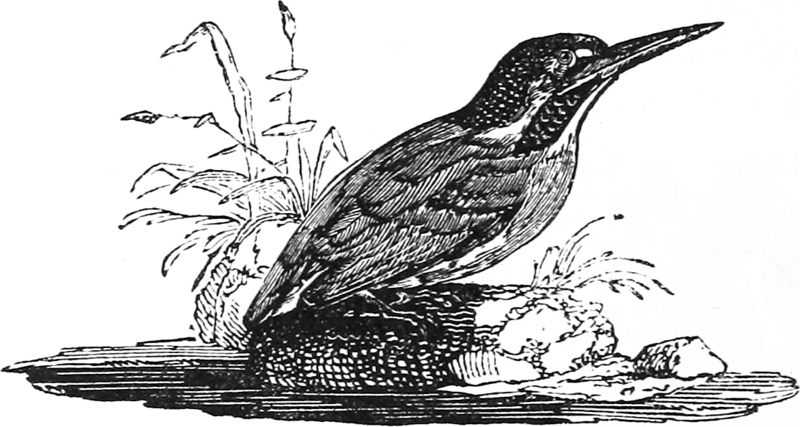
\includegraphics[scale=0.35]{images/Alycon.png}
        \end{figure}
        \vspace{0.5cm}
        \Huge
        \textbf{\textsc{Matematyka Dyskretna}}
        
        \vspace{0.5cm}
        \Large
        \textsc{Wybrane Dowody}
        
        \normalsize
        
        
        \line(1,0){330}
        
        \vspace{1cm}
        \textit{,,Myślę, że 7 punktów na 20 to nie jest zły wynik''}
        \vspace{1cm}

        \textit{\textsc{Popełnione przez}}\\
        \vspace{5mm}

        \textbf{\textsc{Dziurawy Ponton \\ Załatany Ponton \\ Puchaty Pompon \\ Zatopiony Ponton \\ Tonący Ponton \\ Notnop}}

        \vfill

        Kraków \\
        Anno Domini 2023
        
    \end{center}
    
\end{titlepage}


\tableofcontents
\section*{Licencja}
    \begin{figure}[h]
    	\begin{minipage}[c]{0.25\textwidth}
    		
\includegraphics[width=0.7\textwidth]{images/licencja.png}
    	\end{minipage}\hfill
    	\begin{minipage}[c]{0.75\textwidth}
    		\caption*{
    			Ten utwór jest dostępny na 
    			\href{https://creativecommons.org/licenses/by-sa/4.0/}{licencji Creative Commons Uznanie autorstwa
    			na tych samych warunkach 4.0 Międzynarodowe.}
    		}
    	\end{minipage}
    \end{figure}

% Actual content
\mainmatter

\chapter{Kombinatoryka}
 % Żeby nie było syfu to kolejne sekcje dodajemy do chapters/
% A potem includujemy za pomocą \input{chapters/...}

% Używamy \( \) i \[ \] zamiast dolarów -- tak jak się robi w LaTeXu


\documentclass[12pt, a4paper, polish, openany]{book}

% Please, let's familiarize ourselves with notatki.sty and tcs.sty so that we don't reinvent the wheel
\usepackage{notatki}

\fancyhead[L]{\textbf{\textit{MD}}}
\author{
}
\title{TCS and shitposting}


\begin{document}

% Front page and table of contents
\frontmatter

\begin{titlepage} 

    \begin{center}
         \begin{figure}[h]
            \centering
            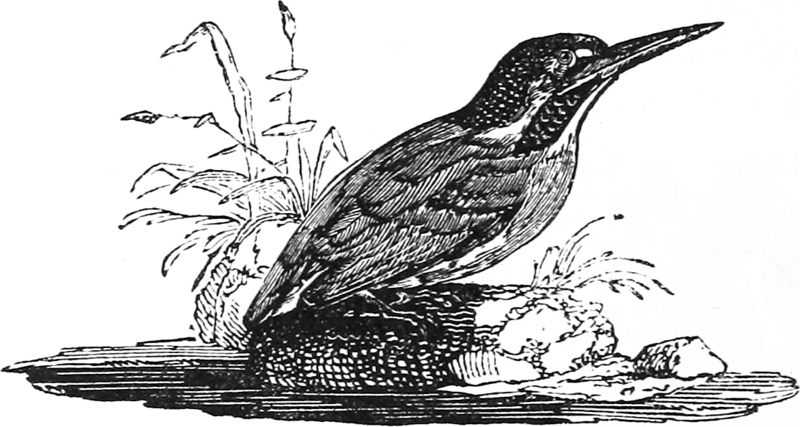
\includegraphics[scale=0.35]{images/Alycon.png}
        \end{figure}
        \vspace{0.5cm}
        \Huge
        \textbf{\textsc{Matematyka Dyskretna}}
        
        \vspace{0.5cm}
        \Large
        \textsc{Wybrane Dowody}
        
        \normalsize
        
        
        \line(1,0){330}
        
        \vspace{1cm}
        \textit{,,Myślę, że 7 punktów na 20 to nie jest zły wynik''}
        \vspace{1cm}

        \textit{\textsc{Popełnione przez}}\\
        \vspace{5mm}

        \textbf{\textsc{Dziurawy Ponton \\ Załatany Ponton \\ Puchaty Pompon \\ Zatopiony Ponton \\ Tonący Ponton \\ Notnop}}

        \vfill

        Kraków \\
        Anno Domini 2023
        
    \end{center}
    
\end{titlepage}


\tableofcontents
\section*{Licencja}
    \begin{figure}[h]
    	\begin{minipage}[c]{0.25\textwidth}
    		
\includegraphics[width=0.7\textwidth]{images/licencja.png}
    	\end{minipage}\hfill
    	\begin{minipage}[c]{0.75\textwidth}
    		\caption*{
    			Ten utwór jest dostępny na 
    			\href{https://creativecommons.org/licenses/by-sa/4.0/}{licencji Creative Commons Uznanie autorstwa
    			na tych samych warunkach 4.0 Międzynarodowe.}
    		}
    	\end{minipage}
    \end{figure}

% Actual content
\mainmatter

\chapter{Kombinatoryka}
 % Żeby nie było syfu to kolejne sekcje dodajemy do chapters/
% A potem includujemy za pomocą \input{chapters/...}

% Używamy \( \) i \[ \] zamiast dolarów -- tak jak się robi w LaTeXu


\documentclass[12pt, a4paper, polish, openany]{book}

% Please, let's familiarize ourselves with notatki.sty and tcs.sty so that we don't reinvent the wheel
\usepackage{notatki}

\fancyhead[L]{\textbf{\textit{MD}}}
\author{
}
\title{TCS and shitposting}


\begin{document}

% Front page and table of contents
\frontmatter

\input{titlepage}

\tableofcontents
\input{license}

% Actual content
\mainmatter

\chapter{Kombinatoryka}
\input{chapters/combinatorics/main}

\chapter{Zasada włączeń i wyłączeń}
\input{chapters/exclusion-inclusion/main}

\chapter{Posety}
\input{chapters/posets/main}

\chapter{Twierdzenie Ramseya}
\input{chapters/ramsey/main}

\chapter{Funkcje tworzące}
\input{chapters/generating_functions/main}

\chapter{Przepływy}
\input{chapters/flows/main}

\chapter{Skojarzenia}
\input{chapters/matchings/main}

\chapter{Kolorowanie grafów}
\input{chapters/graph-coloring/main}

\chapter{Grafy, ale nie kolorowanie}
\input{chapters/graph-misc/main}

\end{document}

\chapter{Zasada włączeń i wyłączeń}
 % Żeby nie było syfu to kolejne sekcje dodajemy do chapters/
% A potem includujemy za pomocą \input{chapters/...}

% Używamy \( \) i \[ \] zamiast dolarów -- tak jak się robi w LaTeXu


\documentclass[12pt, a4paper, polish, openany]{book}

% Please, let's familiarize ourselves with notatki.sty and tcs.sty so that we don't reinvent the wheel
\usepackage{notatki}

\fancyhead[L]{\textbf{\textit{MD}}}
\author{
}
\title{TCS and shitposting}


\begin{document}

% Front page and table of contents
\frontmatter

\input{titlepage}

\tableofcontents
\input{license}

% Actual content
\mainmatter

\chapter{Kombinatoryka}
\input{chapters/combinatorics/main}

\chapter{Zasada włączeń i wyłączeń}
\input{chapters/exclusion-inclusion/main}

\chapter{Posety}
\input{chapters/posets/main}

\chapter{Twierdzenie Ramseya}
\input{chapters/ramsey/main}

\chapter{Funkcje tworzące}
\input{chapters/generating_functions/main}

\chapter{Przepływy}
\input{chapters/flows/main}

\chapter{Skojarzenia}
\input{chapters/matchings/main}

\chapter{Kolorowanie grafów}
\input{chapters/graph-coloring/main}

\chapter{Grafy, ale nie kolorowanie}
\input{chapters/graph-misc/main}

\end{document}

\chapter{Posety}
 % Żeby nie było syfu to kolejne sekcje dodajemy do chapters/
% A potem includujemy za pomocą \input{chapters/...}

% Używamy \( \) i \[ \] zamiast dolarów -- tak jak się robi w LaTeXu


\documentclass[12pt, a4paper, polish, openany]{book}

% Please, let's familiarize ourselves with notatki.sty and tcs.sty so that we don't reinvent the wheel
\usepackage{notatki}

\fancyhead[L]{\textbf{\textit{MD}}}
\author{
}
\title{TCS and shitposting}


\begin{document}

% Front page and table of contents
\frontmatter

\input{titlepage}

\tableofcontents
\input{license}

% Actual content
\mainmatter

\chapter{Kombinatoryka}
\input{chapters/combinatorics/main}

\chapter{Zasada włączeń i wyłączeń}
\input{chapters/exclusion-inclusion/main}

\chapter{Posety}
\input{chapters/posets/main}

\chapter{Twierdzenie Ramseya}
\input{chapters/ramsey/main}

\chapter{Funkcje tworzące}
\input{chapters/generating_functions/main}

\chapter{Przepływy}
\input{chapters/flows/main}

\chapter{Skojarzenia}
\input{chapters/matchings/main}

\chapter{Kolorowanie grafów}
\input{chapters/graph-coloring/main}

\chapter{Grafy, ale nie kolorowanie}
\input{chapters/graph-misc/main}

\end{document}

\chapter{Twierdzenie Ramseya}
 % Żeby nie było syfu to kolejne sekcje dodajemy do chapters/
% A potem includujemy za pomocą \input{chapters/...}

% Używamy \( \) i \[ \] zamiast dolarów -- tak jak się robi w LaTeXu


\documentclass[12pt, a4paper, polish, openany]{book}

% Please, let's familiarize ourselves with notatki.sty and tcs.sty so that we don't reinvent the wheel
\usepackage{notatki}

\fancyhead[L]{\textbf{\textit{MD}}}
\author{
}
\title{TCS and shitposting}


\begin{document}

% Front page and table of contents
\frontmatter

\input{titlepage}

\tableofcontents
\input{license}

% Actual content
\mainmatter

\chapter{Kombinatoryka}
\input{chapters/combinatorics/main}

\chapter{Zasada włączeń i wyłączeń}
\input{chapters/exclusion-inclusion/main}

\chapter{Posety}
\input{chapters/posets/main}

\chapter{Twierdzenie Ramseya}
\input{chapters/ramsey/main}

\chapter{Funkcje tworzące}
\input{chapters/generating_functions/main}

\chapter{Przepływy}
\input{chapters/flows/main}

\chapter{Skojarzenia}
\input{chapters/matchings/main}

\chapter{Kolorowanie grafów}
\input{chapters/graph-coloring/main}

\chapter{Grafy, ale nie kolorowanie}
\input{chapters/graph-misc/main}

\end{document}

\chapter{Funkcje tworzące}
 % Żeby nie było syfu to kolejne sekcje dodajemy do chapters/
% A potem includujemy za pomocą \input{chapters/...}

% Używamy \( \) i \[ \] zamiast dolarów -- tak jak się robi w LaTeXu


\documentclass[12pt, a4paper, polish, openany]{book}

% Please, let's familiarize ourselves with notatki.sty and tcs.sty so that we don't reinvent the wheel
\usepackage{notatki}

\fancyhead[L]{\textbf{\textit{MD}}}
\author{
}
\title{TCS and shitposting}


\begin{document}

% Front page and table of contents
\frontmatter

\input{titlepage}

\tableofcontents
\input{license}

% Actual content
\mainmatter

\chapter{Kombinatoryka}
\input{chapters/combinatorics/main}

\chapter{Zasada włączeń i wyłączeń}
\input{chapters/exclusion-inclusion/main}

\chapter{Posety}
\input{chapters/posets/main}

\chapter{Twierdzenie Ramseya}
\input{chapters/ramsey/main}

\chapter{Funkcje tworzące}
\input{chapters/generating_functions/main}

\chapter{Przepływy}
\input{chapters/flows/main}

\chapter{Skojarzenia}
\input{chapters/matchings/main}

\chapter{Kolorowanie grafów}
\input{chapters/graph-coloring/main}

\chapter{Grafy, ale nie kolorowanie}
\input{chapters/graph-misc/main}

\end{document}

\chapter{Przepływy}
 % Żeby nie było syfu to kolejne sekcje dodajemy do chapters/
% A potem includujemy za pomocą \input{chapters/...}

% Używamy \( \) i \[ \] zamiast dolarów -- tak jak się robi w LaTeXu


\documentclass[12pt, a4paper, polish, openany]{book}

% Please, let's familiarize ourselves with notatki.sty and tcs.sty so that we don't reinvent the wheel
\usepackage{notatki}

\fancyhead[L]{\textbf{\textit{MD}}}
\author{
}
\title{TCS and shitposting}


\begin{document}

% Front page and table of contents
\frontmatter

\input{titlepage}

\tableofcontents
\input{license}

% Actual content
\mainmatter

\chapter{Kombinatoryka}
\input{chapters/combinatorics/main}

\chapter{Zasada włączeń i wyłączeń}
\input{chapters/exclusion-inclusion/main}

\chapter{Posety}
\input{chapters/posets/main}

\chapter{Twierdzenie Ramseya}
\input{chapters/ramsey/main}

\chapter{Funkcje tworzące}
\input{chapters/generating_functions/main}

\chapter{Przepływy}
\input{chapters/flows/main}

\chapter{Skojarzenia}
\input{chapters/matchings/main}

\chapter{Kolorowanie grafów}
\input{chapters/graph-coloring/main}

\chapter{Grafy, ale nie kolorowanie}
\input{chapters/graph-misc/main}

\end{document}

\chapter{Skojarzenia}
 % Żeby nie było syfu to kolejne sekcje dodajemy do chapters/
% A potem includujemy za pomocą \input{chapters/...}

% Używamy \( \) i \[ \] zamiast dolarów -- tak jak się robi w LaTeXu


\documentclass[12pt, a4paper, polish, openany]{book}

% Please, let's familiarize ourselves with notatki.sty and tcs.sty so that we don't reinvent the wheel
\usepackage{notatki}

\fancyhead[L]{\textbf{\textit{MD}}}
\author{
}
\title{TCS and shitposting}


\begin{document}

% Front page and table of contents
\frontmatter

\input{titlepage}

\tableofcontents
\input{license}

% Actual content
\mainmatter

\chapter{Kombinatoryka}
\input{chapters/combinatorics/main}

\chapter{Zasada włączeń i wyłączeń}
\input{chapters/exclusion-inclusion/main}

\chapter{Posety}
\input{chapters/posets/main}

\chapter{Twierdzenie Ramseya}
\input{chapters/ramsey/main}

\chapter{Funkcje tworzące}
\input{chapters/generating_functions/main}

\chapter{Przepływy}
\input{chapters/flows/main}

\chapter{Skojarzenia}
\input{chapters/matchings/main}

\chapter{Kolorowanie grafów}
\input{chapters/graph-coloring/main}

\chapter{Grafy, ale nie kolorowanie}
\input{chapters/graph-misc/main}

\end{document}

\chapter{Kolorowanie grafów}
 % Żeby nie było syfu to kolejne sekcje dodajemy do chapters/
% A potem includujemy za pomocą \input{chapters/...}

% Używamy \( \) i \[ \] zamiast dolarów -- tak jak się robi w LaTeXu


\documentclass[12pt, a4paper, polish, openany]{book}

% Please, let's familiarize ourselves with notatki.sty and tcs.sty so that we don't reinvent the wheel
\usepackage{notatki}

\fancyhead[L]{\textbf{\textit{MD}}}
\author{
}
\title{TCS and shitposting}


\begin{document}

% Front page and table of contents
\frontmatter

\input{titlepage}

\tableofcontents
\input{license}

% Actual content
\mainmatter

\chapter{Kombinatoryka}
\input{chapters/combinatorics/main}

\chapter{Zasada włączeń i wyłączeń}
\input{chapters/exclusion-inclusion/main}

\chapter{Posety}
\input{chapters/posets/main}

\chapter{Twierdzenie Ramseya}
\input{chapters/ramsey/main}

\chapter{Funkcje tworzące}
\input{chapters/generating_functions/main}

\chapter{Przepływy}
\input{chapters/flows/main}

\chapter{Skojarzenia}
\input{chapters/matchings/main}

\chapter{Kolorowanie grafów}
\input{chapters/graph-coloring/main}

\chapter{Grafy, ale nie kolorowanie}
\input{chapters/graph-misc/main}

\end{document}

\chapter{Grafy, ale nie kolorowanie}
 % Żeby nie było syfu to kolejne sekcje dodajemy do chapters/
% A potem includujemy za pomocą \input{chapters/...}

% Używamy \( \) i \[ \] zamiast dolarów -- tak jak się robi w LaTeXu


\documentclass[12pt, a4paper, polish, openany]{book}

% Please, let's familiarize ourselves with notatki.sty and tcs.sty so that we don't reinvent the wheel
\usepackage{notatki}

\fancyhead[L]{\textbf{\textit{MD}}}
\author{
}
\title{TCS and shitposting}


\begin{document}

% Front page and table of contents
\frontmatter

\input{titlepage}

\tableofcontents
\input{license}

% Actual content
\mainmatter

\chapter{Kombinatoryka}
\input{chapters/combinatorics/main}

\chapter{Zasada włączeń i wyłączeń}
\input{chapters/exclusion-inclusion/main}

\chapter{Posety}
\input{chapters/posets/main}

\chapter{Twierdzenie Ramseya}
\input{chapters/ramsey/main}

\chapter{Funkcje tworzące}
\input{chapters/generating_functions/main}

\chapter{Przepływy}
\input{chapters/flows/main}

\chapter{Skojarzenia}
\input{chapters/matchings/main}

\chapter{Kolorowanie grafów}
\input{chapters/graph-coloring/main}

\chapter{Grafy, ale nie kolorowanie}
\input{chapters/graph-misc/main}

\end{document}

\end{document}

\chapter{Zasada włączeń i wyłączeń}
 % Żeby nie było syfu to kolejne sekcje dodajemy do chapters/
% A potem includujemy za pomocą \input{chapters/...}

% Używamy \( \) i \[ \] zamiast dolarów -- tak jak się robi w LaTeXu


\documentclass[12pt, a4paper, polish, openany]{book}

% Please, let's familiarize ourselves with notatki.sty and tcs.sty so that we don't reinvent the wheel
\usepackage{notatki}

\fancyhead[L]{\textbf{\textit{MD}}}
\author{
}
\title{TCS and shitposting}


\begin{document}

% Front page and table of contents
\frontmatter

\begin{titlepage} 

    \begin{center}
         \begin{figure}[h]
            \centering
            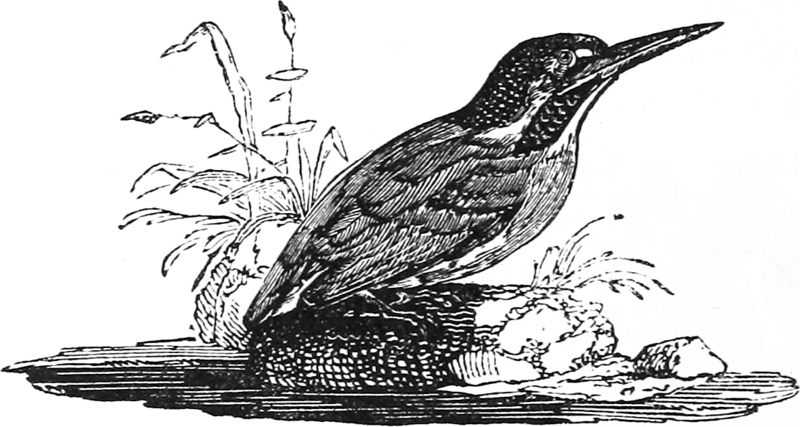
\includegraphics[scale=0.35]{images/Alycon.png}
        \end{figure}
        \vspace{0.5cm}
        \Huge
        \textbf{\textsc{Matematyka Dyskretna}}
        
        \vspace{0.5cm}
        \Large
        \textsc{Wybrane Dowody}
        
        \normalsize
        
        
        \line(1,0){330}
        
        \vspace{1cm}
        \textit{,,Myślę, że 7 punktów na 20 to nie jest zły wynik''}
        \vspace{1cm}

        \textit{\textsc{Popełnione przez}}\\
        \vspace{5mm}

        \textbf{\textsc{Dziurawy Ponton \\ Załatany Ponton \\ Puchaty Pompon \\ Zatopiony Ponton \\ Tonący Ponton \\ Notnop}}

        \vfill

        Kraków \\
        Anno Domini 2023
        
    \end{center}
    
\end{titlepage}


\tableofcontents
\section*{Licencja}
    \begin{figure}[h]
    	\begin{minipage}[c]{0.25\textwidth}
    		
\includegraphics[width=0.7\textwidth]{images/licencja.png}
    	\end{minipage}\hfill
    	\begin{minipage}[c]{0.75\textwidth}
    		\caption*{
    			Ten utwór jest dostępny na 
    			\href{https://creativecommons.org/licenses/by-sa/4.0/}{licencji Creative Commons Uznanie autorstwa
    			na tych samych warunkach 4.0 Międzynarodowe.}
    		}
    	\end{minipage}
    \end{figure}

% Actual content
\mainmatter

\chapter{Kombinatoryka}
 % Żeby nie było syfu to kolejne sekcje dodajemy do chapters/
% A potem includujemy za pomocą \input{chapters/...}

% Używamy \( \) i \[ \] zamiast dolarów -- tak jak się robi w LaTeXu


\documentclass[12pt, a4paper, polish, openany]{book}

% Please, let's familiarize ourselves with notatki.sty and tcs.sty so that we don't reinvent the wheel
\usepackage{notatki}

\fancyhead[L]{\textbf{\textit{MD}}}
\author{
}
\title{TCS and shitposting}


\begin{document}

% Front page and table of contents
\frontmatter

\input{titlepage}

\tableofcontents
\input{license}

% Actual content
\mainmatter

\chapter{Kombinatoryka}
\input{chapters/combinatorics/main}

\chapter{Zasada włączeń i wyłączeń}
\input{chapters/exclusion-inclusion/main}

\chapter{Posety}
\input{chapters/posets/main}

\chapter{Twierdzenie Ramseya}
\input{chapters/ramsey/main}

\chapter{Funkcje tworzące}
\input{chapters/generating_functions/main}

\chapter{Przepływy}
\input{chapters/flows/main}

\chapter{Skojarzenia}
\input{chapters/matchings/main}

\chapter{Kolorowanie grafów}
\input{chapters/graph-coloring/main}

\chapter{Grafy, ale nie kolorowanie}
\input{chapters/graph-misc/main}

\end{document}

\chapter{Zasada włączeń i wyłączeń}
 % Żeby nie było syfu to kolejne sekcje dodajemy do chapters/
% A potem includujemy za pomocą \input{chapters/...}

% Używamy \( \) i \[ \] zamiast dolarów -- tak jak się robi w LaTeXu


\documentclass[12pt, a4paper, polish, openany]{book}

% Please, let's familiarize ourselves with notatki.sty and tcs.sty so that we don't reinvent the wheel
\usepackage{notatki}

\fancyhead[L]{\textbf{\textit{MD}}}
\author{
}
\title{TCS and shitposting}


\begin{document}

% Front page and table of contents
\frontmatter

\input{titlepage}

\tableofcontents
\input{license}

% Actual content
\mainmatter

\chapter{Kombinatoryka}
\input{chapters/combinatorics/main}

\chapter{Zasada włączeń i wyłączeń}
\input{chapters/exclusion-inclusion/main}

\chapter{Posety}
\input{chapters/posets/main}

\chapter{Twierdzenie Ramseya}
\input{chapters/ramsey/main}

\chapter{Funkcje tworzące}
\input{chapters/generating_functions/main}

\chapter{Przepływy}
\input{chapters/flows/main}

\chapter{Skojarzenia}
\input{chapters/matchings/main}

\chapter{Kolorowanie grafów}
\input{chapters/graph-coloring/main}

\chapter{Grafy, ale nie kolorowanie}
\input{chapters/graph-misc/main}

\end{document}

\chapter{Posety}
 % Żeby nie było syfu to kolejne sekcje dodajemy do chapters/
% A potem includujemy za pomocą \input{chapters/...}

% Używamy \( \) i \[ \] zamiast dolarów -- tak jak się robi w LaTeXu


\documentclass[12pt, a4paper, polish, openany]{book}

% Please, let's familiarize ourselves with notatki.sty and tcs.sty so that we don't reinvent the wheel
\usepackage{notatki}

\fancyhead[L]{\textbf{\textit{MD}}}
\author{
}
\title{TCS and shitposting}


\begin{document}

% Front page and table of contents
\frontmatter

\input{titlepage}

\tableofcontents
\input{license}

% Actual content
\mainmatter

\chapter{Kombinatoryka}
\input{chapters/combinatorics/main}

\chapter{Zasada włączeń i wyłączeń}
\input{chapters/exclusion-inclusion/main}

\chapter{Posety}
\input{chapters/posets/main}

\chapter{Twierdzenie Ramseya}
\input{chapters/ramsey/main}

\chapter{Funkcje tworzące}
\input{chapters/generating_functions/main}

\chapter{Przepływy}
\input{chapters/flows/main}

\chapter{Skojarzenia}
\input{chapters/matchings/main}

\chapter{Kolorowanie grafów}
\input{chapters/graph-coloring/main}

\chapter{Grafy, ale nie kolorowanie}
\input{chapters/graph-misc/main}

\end{document}

\chapter{Twierdzenie Ramseya}
 % Żeby nie było syfu to kolejne sekcje dodajemy do chapters/
% A potem includujemy za pomocą \input{chapters/...}

% Używamy \( \) i \[ \] zamiast dolarów -- tak jak się robi w LaTeXu


\documentclass[12pt, a4paper, polish, openany]{book}

% Please, let's familiarize ourselves with notatki.sty and tcs.sty so that we don't reinvent the wheel
\usepackage{notatki}

\fancyhead[L]{\textbf{\textit{MD}}}
\author{
}
\title{TCS and shitposting}


\begin{document}

% Front page and table of contents
\frontmatter

\input{titlepage}

\tableofcontents
\input{license}

% Actual content
\mainmatter

\chapter{Kombinatoryka}
\input{chapters/combinatorics/main}

\chapter{Zasada włączeń i wyłączeń}
\input{chapters/exclusion-inclusion/main}

\chapter{Posety}
\input{chapters/posets/main}

\chapter{Twierdzenie Ramseya}
\input{chapters/ramsey/main}

\chapter{Funkcje tworzące}
\input{chapters/generating_functions/main}

\chapter{Przepływy}
\input{chapters/flows/main}

\chapter{Skojarzenia}
\input{chapters/matchings/main}

\chapter{Kolorowanie grafów}
\input{chapters/graph-coloring/main}

\chapter{Grafy, ale nie kolorowanie}
\input{chapters/graph-misc/main}

\end{document}

\chapter{Funkcje tworzące}
 % Żeby nie było syfu to kolejne sekcje dodajemy do chapters/
% A potem includujemy za pomocą \input{chapters/...}

% Używamy \( \) i \[ \] zamiast dolarów -- tak jak się robi w LaTeXu


\documentclass[12pt, a4paper, polish, openany]{book}

% Please, let's familiarize ourselves with notatki.sty and tcs.sty so that we don't reinvent the wheel
\usepackage{notatki}

\fancyhead[L]{\textbf{\textit{MD}}}
\author{
}
\title{TCS and shitposting}


\begin{document}

% Front page and table of contents
\frontmatter

\input{titlepage}

\tableofcontents
\input{license}

% Actual content
\mainmatter

\chapter{Kombinatoryka}
\input{chapters/combinatorics/main}

\chapter{Zasada włączeń i wyłączeń}
\input{chapters/exclusion-inclusion/main}

\chapter{Posety}
\input{chapters/posets/main}

\chapter{Twierdzenie Ramseya}
\input{chapters/ramsey/main}

\chapter{Funkcje tworzące}
\input{chapters/generating_functions/main}

\chapter{Przepływy}
\input{chapters/flows/main}

\chapter{Skojarzenia}
\input{chapters/matchings/main}

\chapter{Kolorowanie grafów}
\input{chapters/graph-coloring/main}

\chapter{Grafy, ale nie kolorowanie}
\input{chapters/graph-misc/main}

\end{document}

\chapter{Przepływy}
 % Żeby nie było syfu to kolejne sekcje dodajemy do chapters/
% A potem includujemy za pomocą \input{chapters/...}

% Używamy \( \) i \[ \] zamiast dolarów -- tak jak się robi w LaTeXu


\documentclass[12pt, a4paper, polish, openany]{book}

% Please, let's familiarize ourselves with notatki.sty and tcs.sty so that we don't reinvent the wheel
\usepackage{notatki}

\fancyhead[L]{\textbf{\textit{MD}}}
\author{
}
\title{TCS and shitposting}


\begin{document}

% Front page and table of contents
\frontmatter

\input{titlepage}

\tableofcontents
\input{license}

% Actual content
\mainmatter

\chapter{Kombinatoryka}
\input{chapters/combinatorics/main}

\chapter{Zasada włączeń i wyłączeń}
\input{chapters/exclusion-inclusion/main}

\chapter{Posety}
\input{chapters/posets/main}

\chapter{Twierdzenie Ramseya}
\input{chapters/ramsey/main}

\chapter{Funkcje tworzące}
\input{chapters/generating_functions/main}

\chapter{Przepływy}
\input{chapters/flows/main}

\chapter{Skojarzenia}
\input{chapters/matchings/main}

\chapter{Kolorowanie grafów}
\input{chapters/graph-coloring/main}

\chapter{Grafy, ale nie kolorowanie}
\input{chapters/graph-misc/main}

\end{document}

\chapter{Skojarzenia}
 % Żeby nie było syfu to kolejne sekcje dodajemy do chapters/
% A potem includujemy za pomocą \input{chapters/...}

% Używamy \( \) i \[ \] zamiast dolarów -- tak jak się robi w LaTeXu


\documentclass[12pt, a4paper, polish, openany]{book}

% Please, let's familiarize ourselves with notatki.sty and tcs.sty so that we don't reinvent the wheel
\usepackage{notatki}

\fancyhead[L]{\textbf{\textit{MD}}}
\author{
}
\title{TCS and shitposting}


\begin{document}

% Front page and table of contents
\frontmatter

\input{titlepage}

\tableofcontents
\input{license}

% Actual content
\mainmatter

\chapter{Kombinatoryka}
\input{chapters/combinatorics/main}

\chapter{Zasada włączeń i wyłączeń}
\input{chapters/exclusion-inclusion/main}

\chapter{Posety}
\input{chapters/posets/main}

\chapter{Twierdzenie Ramseya}
\input{chapters/ramsey/main}

\chapter{Funkcje tworzące}
\input{chapters/generating_functions/main}

\chapter{Przepływy}
\input{chapters/flows/main}

\chapter{Skojarzenia}
\input{chapters/matchings/main}

\chapter{Kolorowanie grafów}
\input{chapters/graph-coloring/main}

\chapter{Grafy, ale nie kolorowanie}
\input{chapters/graph-misc/main}

\end{document}

\chapter{Kolorowanie grafów}
 % Żeby nie było syfu to kolejne sekcje dodajemy do chapters/
% A potem includujemy za pomocą \input{chapters/...}

% Używamy \( \) i \[ \] zamiast dolarów -- tak jak się robi w LaTeXu


\documentclass[12pt, a4paper, polish, openany]{book}

% Please, let's familiarize ourselves with notatki.sty and tcs.sty so that we don't reinvent the wheel
\usepackage{notatki}

\fancyhead[L]{\textbf{\textit{MD}}}
\author{
}
\title{TCS and shitposting}


\begin{document}

% Front page and table of contents
\frontmatter

\input{titlepage}

\tableofcontents
\input{license}

% Actual content
\mainmatter

\chapter{Kombinatoryka}
\input{chapters/combinatorics/main}

\chapter{Zasada włączeń i wyłączeń}
\input{chapters/exclusion-inclusion/main}

\chapter{Posety}
\input{chapters/posets/main}

\chapter{Twierdzenie Ramseya}
\input{chapters/ramsey/main}

\chapter{Funkcje tworzące}
\input{chapters/generating_functions/main}

\chapter{Przepływy}
\input{chapters/flows/main}

\chapter{Skojarzenia}
\input{chapters/matchings/main}

\chapter{Kolorowanie grafów}
\input{chapters/graph-coloring/main}

\chapter{Grafy, ale nie kolorowanie}
\input{chapters/graph-misc/main}

\end{document}

\chapter{Grafy, ale nie kolorowanie}
 % Żeby nie było syfu to kolejne sekcje dodajemy do chapters/
% A potem includujemy za pomocą \input{chapters/...}

% Używamy \( \) i \[ \] zamiast dolarów -- tak jak się robi w LaTeXu


\documentclass[12pt, a4paper, polish, openany]{book}

% Please, let's familiarize ourselves with notatki.sty and tcs.sty so that we don't reinvent the wheel
\usepackage{notatki}

\fancyhead[L]{\textbf{\textit{MD}}}
\author{
}
\title{TCS and shitposting}


\begin{document}

% Front page and table of contents
\frontmatter

\input{titlepage}

\tableofcontents
\input{license}

% Actual content
\mainmatter

\chapter{Kombinatoryka}
\input{chapters/combinatorics/main}

\chapter{Zasada włączeń i wyłączeń}
\input{chapters/exclusion-inclusion/main}

\chapter{Posety}
\input{chapters/posets/main}

\chapter{Twierdzenie Ramseya}
\input{chapters/ramsey/main}

\chapter{Funkcje tworzące}
\input{chapters/generating_functions/main}

\chapter{Przepływy}
\input{chapters/flows/main}

\chapter{Skojarzenia}
\input{chapters/matchings/main}

\chapter{Kolorowanie grafów}
\input{chapters/graph-coloring/main}

\chapter{Grafy, ale nie kolorowanie}
\input{chapters/graph-misc/main}

\end{document}

\end{document}

\chapter{Posety}
 % Żeby nie było syfu to kolejne sekcje dodajemy do chapters/
% A potem includujemy za pomocą \input{chapters/...}

% Używamy \( \) i \[ \] zamiast dolarów -- tak jak się robi w LaTeXu


\documentclass[12pt, a4paper, polish, openany]{book}

% Please, let's familiarize ourselves with notatki.sty and tcs.sty so that we don't reinvent the wheel
\usepackage{notatki}

\fancyhead[L]{\textbf{\textit{MD}}}
\author{
}
\title{TCS and shitposting}


\begin{document}

% Front page and table of contents
\frontmatter

\begin{titlepage} 

    \begin{center}
         \begin{figure}[h]
            \centering
            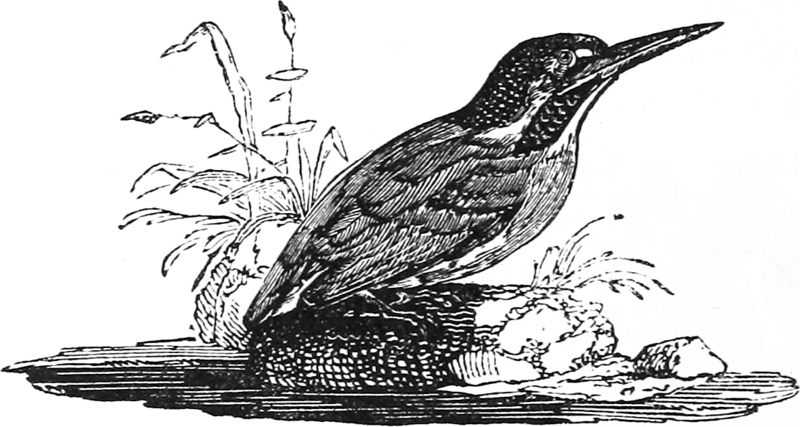
\includegraphics[scale=0.35]{images/Alycon.png}
        \end{figure}
        \vspace{0.5cm}
        \Huge
        \textbf{\textsc{Matematyka Dyskretna}}
        
        \vspace{0.5cm}
        \Large
        \textsc{Wybrane Dowody}
        
        \normalsize
        
        
        \line(1,0){330}
        
        \vspace{1cm}
        \textit{,,Myślę, że 7 punktów na 20 to nie jest zły wynik''}
        \vspace{1cm}

        \textit{\textsc{Popełnione przez}}\\
        \vspace{5mm}

        \textbf{\textsc{Dziurawy Ponton \\ Załatany Ponton \\ Puchaty Pompon \\ Zatopiony Ponton \\ Tonący Ponton \\ Notnop}}

        \vfill

        Kraków \\
        Anno Domini 2023
        
    \end{center}
    
\end{titlepage}


\tableofcontents
\section*{Licencja}
    \begin{figure}[h]
    	\begin{minipage}[c]{0.25\textwidth}
    		
\includegraphics[width=0.7\textwidth]{images/licencja.png}
    	\end{minipage}\hfill
    	\begin{minipage}[c]{0.75\textwidth}
    		\caption*{
    			Ten utwór jest dostępny na 
    			\href{https://creativecommons.org/licenses/by-sa/4.0/}{licencji Creative Commons Uznanie autorstwa
    			na tych samych warunkach 4.0 Międzynarodowe.}
    		}
    	\end{minipage}
    \end{figure}

% Actual content
\mainmatter

\chapter{Kombinatoryka}
 % Żeby nie było syfu to kolejne sekcje dodajemy do chapters/
% A potem includujemy za pomocą \input{chapters/...}

% Używamy \( \) i \[ \] zamiast dolarów -- tak jak się robi w LaTeXu


\documentclass[12pt, a4paper, polish, openany]{book}

% Please, let's familiarize ourselves with notatki.sty and tcs.sty so that we don't reinvent the wheel
\usepackage{notatki}

\fancyhead[L]{\textbf{\textit{MD}}}
\author{
}
\title{TCS and shitposting}


\begin{document}

% Front page and table of contents
\frontmatter

\input{titlepage}

\tableofcontents
\input{license}

% Actual content
\mainmatter

\chapter{Kombinatoryka}
\input{chapters/combinatorics/main}

\chapter{Zasada włączeń i wyłączeń}
\input{chapters/exclusion-inclusion/main}

\chapter{Posety}
\input{chapters/posets/main}

\chapter{Twierdzenie Ramseya}
\input{chapters/ramsey/main}

\chapter{Funkcje tworzące}
\input{chapters/generating_functions/main}

\chapter{Przepływy}
\input{chapters/flows/main}

\chapter{Skojarzenia}
\input{chapters/matchings/main}

\chapter{Kolorowanie grafów}
\input{chapters/graph-coloring/main}

\chapter{Grafy, ale nie kolorowanie}
\input{chapters/graph-misc/main}

\end{document}

\chapter{Zasada włączeń i wyłączeń}
 % Żeby nie było syfu to kolejne sekcje dodajemy do chapters/
% A potem includujemy za pomocą \input{chapters/...}

% Używamy \( \) i \[ \] zamiast dolarów -- tak jak się robi w LaTeXu


\documentclass[12pt, a4paper, polish, openany]{book}

% Please, let's familiarize ourselves with notatki.sty and tcs.sty so that we don't reinvent the wheel
\usepackage{notatki}

\fancyhead[L]{\textbf{\textit{MD}}}
\author{
}
\title{TCS and shitposting}


\begin{document}

% Front page and table of contents
\frontmatter

\input{titlepage}

\tableofcontents
\input{license}

% Actual content
\mainmatter

\chapter{Kombinatoryka}
\input{chapters/combinatorics/main}

\chapter{Zasada włączeń i wyłączeń}
\input{chapters/exclusion-inclusion/main}

\chapter{Posety}
\input{chapters/posets/main}

\chapter{Twierdzenie Ramseya}
\input{chapters/ramsey/main}

\chapter{Funkcje tworzące}
\input{chapters/generating_functions/main}

\chapter{Przepływy}
\input{chapters/flows/main}

\chapter{Skojarzenia}
\input{chapters/matchings/main}

\chapter{Kolorowanie grafów}
\input{chapters/graph-coloring/main}

\chapter{Grafy, ale nie kolorowanie}
\input{chapters/graph-misc/main}

\end{document}

\chapter{Posety}
 % Żeby nie było syfu to kolejne sekcje dodajemy do chapters/
% A potem includujemy za pomocą \input{chapters/...}

% Używamy \( \) i \[ \] zamiast dolarów -- tak jak się robi w LaTeXu


\documentclass[12pt, a4paper, polish, openany]{book}

% Please, let's familiarize ourselves with notatki.sty and tcs.sty so that we don't reinvent the wheel
\usepackage{notatki}

\fancyhead[L]{\textbf{\textit{MD}}}
\author{
}
\title{TCS and shitposting}


\begin{document}

% Front page and table of contents
\frontmatter

\input{titlepage}

\tableofcontents
\input{license}

% Actual content
\mainmatter

\chapter{Kombinatoryka}
\input{chapters/combinatorics/main}

\chapter{Zasada włączeń i wyłączeń}
\input{chapters/exclusion-inclusion/main}

\chapter{Posety}
\input{chapters/posets/main}

\chapter{Twierdzenie Ramseya}
\input{chapters/ramsey/main}

\chapter{Funkcje tworzące}
\input{chapters/generating_functions/main}

\chapter{Przepływy}
\input{chapters/flows/main}

\chapter{Skojarzenia}
\input{chapters/matchings/main}

\chapter{Kolorowanie grafów}
\input{chapters/graph-coloring/main}

\chapter{Grafy, ale nie kolorowanie}
\input{chapters/graph-misc/main}

\end{document}

\chapter{Twierdzenie Ramseya}
 % Żeby nie było syfu to kolejne sekcje dodajemy do chapters/
% A potem includujemy za pomocą \input{chapters/...}

% Używamy \( \) i \[ \] zamiast dolarów -- tak jak się robi w LaTeXu


\documentclass[12pt, a4paper, polish, openany]{book}

% Please, let's familiarize ourselves with notatki.sty and tcs.sty so that we don't reinvent the wheel
\usepackage{notatki}

\fancyhead[L]{\textbf{\textit{MD}}}
\author{
}
\title{TCS and shitposting}


\begin{document}

% Front page and table of contents
\frontmatter

\input{titlepage}

\tableofcontents
\input{license}

% Actual content
\mainmatter

\chapter{Kombinatoryka}
\input{chapters/combinatorics/main}

\chapter{Zasada włączeń i wyłączeń}
\input{chapters/exclusion-inclusion/main}

\chapter{Posety}
\input{chapters/posets/main}

\chapter{Twierdzenie Ramseya}
\input{chapters/ramsey/main}

\chapter{Funkcje tworzące}
\input{chapters/generating_functions/main}

\chapter{Przepływy}
\input{chapters/flows/main}

\chapter{Skojarzenia}
\input{chapters/matchings/main}

\chapter{Kolorowanie grafów}
\input{chapters/graph-coloring/main}

\chapter{Grafy, ale nie kolorowanie}
\input{chapters/graph-misc/main}

\end{document}

\chapter{Funkcje tworzące}
 % Żeby nie było syfu to kolejne sekcje dodajemy do chapters/
% A potem includujemy za pomocą \input{chapters/...}

% Używamy \( \) i \[ \] zamiast dolarów -- tak jak się robi w LaTeXu


\documentclass[12pt, a4paper, polish, openany]{book}

% Please, let's familiarize ourselves with notatki.sty and tcs.sty so that we don't reinvent the wheel
\usepackage{notatki}

\fancyhead[L]{\textbf{\textit{MD}}}
\author{
}
\title{TCS and shitposting}


\begin{document}

% Front page and table of contents
\frontmatter

\input{titlepage}

\tableofcontents
\input{license}

% Actual content
\mainmatter

\chapter{Kombinatoryka}
\input{chapters/combinatorics/main}

\chapter{Zasada włączeń i wyłączeń}
\input{chapters/exclusion-inclusion/main}

\chapter{Posety}
\input{chapters/posets/main}

\chapter{Twierdzenie Ramseya}
\input{chapters/ramsey/main}

\chapter{Funkcje tworzące}
\input{chapters/generating_functions/main}

\chapter{Przepływy}
\input{chapters/flows/main}

\chapter{Skojarzenia}
\input{chapters/matchings/main}

\chapter{Kolorowanie grafów}
\input{chapters/graph-coloring/main}

\chapter{Grafy, ale nie kolorowanie}
\input{chapters/graph-misc/main}

\end{document}

\chapter{Przepływy}
 % Żeby nie było syfu to kolejne sekcje dodajemy do chapters/
% A potem includujemy za pomocą \input{chapters/...}

% Używamy \( \) i \[ \] zamiast dolarów -- tak jak się robi w LaTeXu


\documentclass[12pt, a4paper, polish, openany]{book}

% Please, let's familiarize ourselves with notatki.sty and tcs.sty so that we don't reinvent the wheel
\usepackage{notatki}

\fancyhead[L]{\textbf{\textit{MD}}}
\author{
}
\title{TCS and shitposting}


\begin{document}

% Front page and table of contents
\frontmatter

\input{titlepage}

\tableofcontents
\input{license}

% Actual content
\mainmatter

\chapter{Kombinatoryka}
\input{chapters/combinatorics/main}

\chapter{Zasada włączeń i wyłączeń}
\input{chapters/exclusion-inclusion/main}

\chapter{Posety}
\input{chapters/posets/main}

\chapter{Twierdzenie Ramseya}
\input{chapters/ramsey/main}

\chapter{Funkcje tworzące}
\input{chapters/generating_functions/main}

\chapter{Przepływy}
\input{chapters/flows/main}

\chapter{Skojarzenia}
\input{chapters/matchings/main}

\chapter{Kolorowanie grafów}
\input{chapters/graph-coloring/main}

\chapter{Grafy, ale nie kolorowanie}
\input{chapters/graph-misc/main}

\end{document}

\chapter{Skojarzenia}
 % Żeby nie było syfu to kolejne sekcje dodajemy do chapters/
% A potem includujemy za pomocą \input{chapters/...}

% Używamy \( \) i \[ \] zamiast dolarów -- tak jak się robi w LaTeXu


\documentclass[12pt, a4paper, polish, openany]{book}

% Please, let's familiarize ourselves with notatki.sty and tcs.sty so that we don't reinvent the wheel
\usepackage{notatki}

\fancyhead[L]{\textbf{\textit{MD}}}
\author{
}
\title{TCS and shitposting}


\begin{document}

% Front page and table of contents
\frontmatter

\input{titlepage}

\tableofcontents
\input{license}

% Actual content
\mainmatter

\chapter{Kombinatoryka}
\input{chapters/combinatorics/main}

\chapter{Zasada włączeń i wyłączeń}
\input{chapters/exclusion-inclusion/main}

\chapter{Posety}
\input{chapters/posets/main}

\chapter{Twierdzenie Ramseya}
\input{chapters/ramsey/main}

\chapter{Funkcje tworzące}
\input{chapters/generating_functions/main}

\chapter{Przepływy}
\input{chapters/flows/main}

\chapter{Skojarzenia}
\input{chapters/matchings/main}

\chapter{Kolorowanie grafów}
\input{chapters/graph-coloring/main}

\chapter{Grafy, ale nie kolorowanie}
\input{chapters/graph-misc/main}

\end{document}

\chapter{Kolorowanie grafów}
 % Żeby nie było syfu to kolejne sekcje dodajemy do chapters/
% A potem includujemy za pomocą \input{chapters/...}

% Używamy \( \) i \[ \] zamiast dolarów -- tak jak się robi w LaTeXu


\documentclass[12pt, a4paper, polish, openany]{book}

% Please, let's familiarize ourselves with notatki.sty and tcs.sty so that we don't reinvent the wheel
\usepackage{notatki}

\fancyhead[L]{\textbf{\textit{MD}}}
\author{
}
\title{TCS and shitposting}


\begin{document}

% Front page and table of contents
\frontmatter

\input{titlepage}

\tableofcontents
\input{license}

% Actual content
\mainmatter

\chapter{Kombinatoryka}
\input{chapters/combinatorics/main}

\chapter{Zasada włączeń i wyłączeń}
\input{chapters/exclusion-inclusion/main}

\chapter{Posety}
\input{chapters/posets/main}

\chapter{Twierdzenie Ramseya}
\input{chapters/ramsey/main}

\chapter{Funkcje tworzące}
\input{chapters/generating_functions/main}

\chapter{Przepływy}
\input{chapters/flows/main}

\chapter{Skojarzenia}
\input{chapters/matchings/main}

\chapter{Kolorowanie grafów}
\input{chapters/graph-coloring/main}

\chapter{Grafy, ale nie kolorowanie}
\input{chapters/graph-misc/main}

\end{document}

\chapter{Grafy, ale nie kolorowanie}
 % Żeby nie było syfu to kolejne sekcje dodajemy do chapters/
% A potem includujemy za pomocą \input{chapters/...}

% Używamy \( \) i \[ \] zamiast dolarów -- tak jak się robi w LaTeXu


\documentclass[12pt, a4paper, polish, openany]{book}

% Please, let's familiarize ourselves with notatki.sty and tcs.sty so that we don't reinvent the wheel
\usepackage{notatki}

\fancyhead[L]{\textbf{\textit{MD}}}
\author{
}
\title{TCS and shitposting}


\begin{document}

% Front page and table of contents
\frontmatter

\input{titlepage}

\tableofcontents
\input{license}

% Actual content
\mainmatter

\chapter{Kombinatoryka}
\input{chapters/combinatorics/main}

\chapter{Zasada włączeń i wyłączeń}
\input{chapters/exclusion-inclusion/main}

\chapter{Posety}
\input{chapters/posets/main}

\chapter{Twierdzenie Ramseya}
\input{chapters/ramsey/main}

\chapter{Funkcje tworzące}
\input{chapters/generating_functions/main}

\chapter{Przepływy}
\input{chapters/flows/main}

\chapter{Skojarzenia}
\input{chapters/matchings/main}

\chapter{Kolorowanie grafów}
\input{chapters/graph-coloring/main}

\chapter{Grafy, ale nie kolorowanie}
\input{chapters/graph-misc/main}

\end{document}

\end{document}

\chapter{Twierdzenie Ramseya}
 % Żeby nie było syfu to kolejne sekcje dodajemy do chapters/
% A potem includujemy za pomocą \input{chapters/...}

% Używamy \( \) i \[ \] zamiast dolarów -- tak jak się robi w LaTeXu


\documentclass[12pt, a4paper, polish, openany]{book}

% Please, let's familiarize ourselves with notatki.sty and tcs.sty so that we don't reinvent the wheel
\usepackage{notatki}

\fancyhead[L]{\textbf{\textit{MD}}}
\author{
}
\title{TCS and shitposting}


\begin{document}

% Front page and table of contents
\frontmatter

\begin{titlepage} 

    \begin{center}
         \begin{figure}[h]
            \centering
            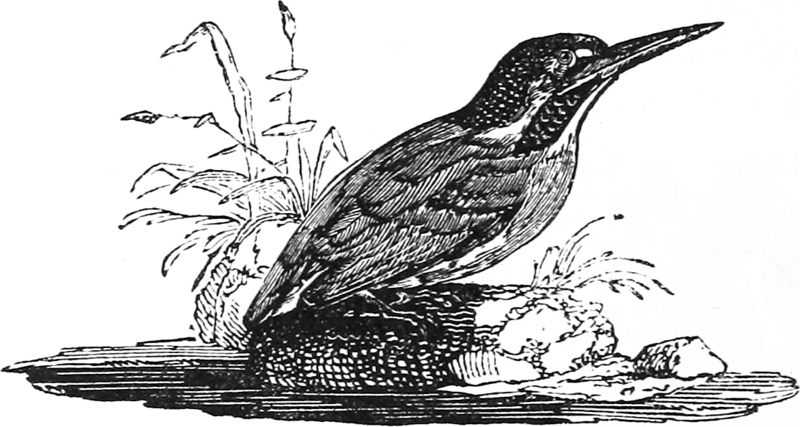
\includegraphics[scale=0.35]{images/Alycon.png}
        \end{figure}
        \vspace{0.5cm}
        \Huge
        \textbf{\textsc{Matematyka Dyskretna}}
        
        \vspace{0.5cm}
        \Large
        \textsc{Wybrane Dowody}
        
        \normalsize
        
        
        \line(1,0){330}
        
        \vspace{1cm}
        \textit{,,Myślę, że 7 punktów na 20 to nie jest zły wynik''}
        \vspace{1cm}

        \textit{\textsc{Popełnione przez}}\\
        \vspace{5mm}

        \textbf{\textsc{Dziurawy Ponton \\ Załatany Ponton \\ Puchaty Pompon \\ Zatopiony Ponton \\ Tonący Ponton \\ Notnop}}

        \vfill

        Kraków \\
        Anno Domini 2023
        
    \end{center}
    
\end{titlepage}


\tableofcontents
\section*{Licencja}
    \begin{figure}[h]
    	\begin{minipage}[c]{0.25\textwidth}
    		
\includegraphics[width=0.7\textwidth]{images/licencja.png}
    	\end{minipage}\hfill
    	\begin{minipage}[c]{0.75\textwidth}
    		\caption*{
    			Ten utwór jest dostępny na 
    			\href{https://creativecommons.org/licenses/by-sa/4.0/}{licencji Creative Commons Uznanie autorstwa
    			na tych samych warunkach 4.0 Międzynarodowe.}
    		}
    	\end{minipage}
    \end{figure}

% Actual content
\mainmatter

\chapter{Kombinatoryka}
 % Żeby nie było syfu to kolejne sekcje dodajemy do chapters/
% A potem includujemy za pomocą \input{chapters/...}

% Używamy \( \) i \[ \] zamiast dolarów -- tak jak się robi w LaTeXu


\documentclass[12pt, a4paper, polish, openany]{book}

% Please, let's familiarize ourselves with notatki.sty and tcs.sty so that we don't reinvent the wheel
\usepackage{notatki}

\fancyhead[L]{\textbf{\textit{MD}}}
\author{
}
\title{TCS and shitposting}


\begin{document}

% Front page and table of contents
\frontmatter

\input{titlepage}

\tableofcontents
\input{license}

% Actual content
\mainmatter

\chapter{Kombinatoryka}
\input{chapters/combinatorics/main}

\chapter{Zasada włączeń i wyłączeń}
\input{chapters/exclusion-inclusion/main}

\chapter{Posety}
\input{chapters/posets/main}

\chapter{Twierdzenie Ramseya}
\input{chapters/ramsey/main}

\chapter{Funkcje tworzące}
\input{chapters/generating_functions/main}

\chapter{Przepływy}
\input{chapters/flows/main}

\chapter{Skojarzenia}
\input{chapters/matchings/main}

\chapter{Kolorowanie grafów}
\input{chapters/graph-coloring/main}

\chapter{Grafy, ale nie kolorowanie}
\input{chapters/graph-misc/main}

\end{document}

\chapter{Zasada włączeń i wyłączeń}
 % Żeby nie było syfu to kolejne sekcje dodajemy do chapters/
% A potem includujemy za pomocą \input{chapters/...}

% Używamy \( \) i \[ \] zamiast dolarów -- tak jak się robi w LaTeXu


\documentclass[12pt, a4paper, polish, openany]{book}

% Please, let's familiarize ourselves with notatki.sty and tcs.sty so that we don't reinvent the wheel
\usepackage{notatki}

\fancyhead[L]{\textbf{\textit{MD}}}
\author{
}
\title{TCS and shitposting}


\begin{document}

% Front page and table of contents
\frontmatter

\input{titlepage}

\tableofcontents
\input{license}

% Actual content
\mainmatter

\chapter{Kombinatoryka}
\input{chapters/combinatorics/main}

\chapter{Zasada włączeń i wyłączeń}
\input{chapters/exclusion-inclusion/main}

\chapter{Posety}
\input{chapters/posets/main}

\chapter{Twierdzenie Ramseya}
\input{chapters/ramsey/main}

\chapter{Funkcje tworzące}
\input{chapters/generating_functions/main}

\chapter{Przepływy}
\input{chapters/flows/main}

\chapter{Skojarzenia}
\input{chapters/matchings/main}

\chapter{Kolorowanie grafów}
\input{chapters/graph-coloring/main}

\chapter{Grafy, ale nie kolorowanie}
\input{chapters/graph-misc/main}

\end{document}

\chapter{Posety}
 % Żeby nie było syfu to kolejne sekcje dodajemy do chapters/
% A potem includujemy za pomocą \input{chapters/...}

% Używamy \( \) i \[ \] zamiast dolarów -- tak jak się robi w LaTeXu


\documentclass[12pt, a4paper, polish, openany]{book}

% Please, let's familiarize ourselves with notatki.sty and tcs.sty so that we don't reinvent the wheel
\usepackage{notatki}

\fancyhead[L]{\textbf{\textit{MD}}}
\author{
}
\title{TCS and shitposting}


\begin{document}

% Front page and table of contents
\frontmatter

\input{titlepage}

\tableofcontents
\input{license}

% Actual content
\mainmatter

\chapter{Kombinatoryka}
\input{chapters/combinatorics/main}

\chapter{Zasada włączeń i wyłączeń}
\input{chapters/exclusion-inclusion/main}

\chapter{Posety}
\input{chapters/posets/main}

\chapter{Twierdzenie Ramseya}
\input{chapters/ramsey/main}

\chapter{Funkcje tworzące}
\input{chapters/generating_functions/main}

\chapter{Przepływy}
\input{chapters/flows/main}

\chapter{Skojarzenia}
\input{chapters/matchings/main}

\chapter{Kolorowanie grafów}
\input{chapters/graph-coloring/main}

\chapter{Grafy, ale nie kolorowanie}
\input{chapters/graph-misc/main}

\end{document}

\chapter{Twierdzenie Ramseya}
 % Żeby nie było syfu to kolejne sekcje dodajemy do chapters/
% A potem includujemy za pomocą \input{chapters/...}

% Używamy \( \) i \[ \] zamiast dolarów -- tak jak się robi w LaTeXu


\documentclass[12pt, a4paper, polish, openany]{book}

% Please, let's familiarize ourselves with notatki.sty and tcs.sty so that we don't reinvent the wheel
\usepackage{notatki}

\fancyhead[L]{\textbf{\textit{MD}}}
\author{
}
\title{TCS and shitposting}


\begin{document}

% Front page and table of contents
\frontmatter

\input{titlepage}

\tableofcontents
\input{license}

% Actual content
\mainmatter

\chapter{Kombinatoryka}
\input{chapters/combinatorics/main}

\chapter{Zasada włączeń i wyłączeń}
\input{chapters/exclusion-inclusion/main}

\chapter{Posety}
\input{chapters/posets/main}

\chapter{Twierdzenie Ramseya}
\input{chapters/ramsey/main}

\chapter{Funkcje tworzące}
\input{chapters/generating_functions/main}

\chapter{Przepływy}
\input{chapters/flows/main}

\chapter{Skojarzenia}
\input{chapters/matchings/main}

\chapter{Kolorowanie grafów}
\input{chapters/graph-coloring/main}

\chapter{Grafy, ale nie kolorowanie}
\input{chapters/graph-misc/main}

\end{document}

\chapter{Funkcje tworzące}
 % Żeby nie było syfu to kolejne sekcje dodajemy do chapters/
% A potem includujemy za pomocą \input{chapters/...}

% Używamy \( \) i \[ \] zamiast dolarów -- tak jak się robi w LaTeXu


\documentclass[12pt, a4paper, polish, openany]{book}

% Please, let's familiarize ourselves with notatki.sty and tcs.sty so that we don't reinvent the wheel
\usepackage{notatki}

\fancyhead[L]{\textbf{\textit{MD}}}
\author{
}
\title{TCS and shitposting}


\begin{document}

% Front page and table of contents
\frontmatter

\input{titlepage}

\tableofcontents
\input{license}

% Actual content
\mainmatter

\chapter{Kombinatoryka}
\input{chapters/combinatorics/main}

\chapter{Zasada włączeń i wyłączeń}
\input{chapters/exclusion-inclusion/main}

\chapter{Posety}
\input{chapters/posets/main}

\chapter{Twierdzenie Ramseya}
\input{chapters/ramsey/main}

\chapter{Funkcje tworzące}
\input{chapters/generating_functions/main}

\chapter{Przepływy}
\input{chapters/flows/main}

\chapter{Skojarzenia}
\input{chapters/matchings/main}

\chapter{Kolorowanie grafów}
\input{chapters/graph-coloring/main}

\chapter{Grafy, ale nie kolorowanie}
\input{chapters/graph-misc/main}

\end{document}

\chapter{Przepływy}
 % Żeby nie było syfu to kolejne sekcje dodajemy do chapters/
% A potem includujemy za pomocą \input{chapters/...}

% Używamy \( \) i \[ \] zamiast dolarów -- tak jak się robi w LaTeXu


\documentclass[12pt, a4paper, polish, openany]{book}

% Please, let's familiarize ourselves with notatki.sty and tcs.sty so that we don't reinvent the wheel
\usepackage{notatki}

\fancyhead[L]{\textbf{\textit{MD}}}
\author{
}
\title{TCS and shitposting}


\begin{document}

% Front page and table of contents
\frontmatter

\input{titlepage}

\tableofcontents
\input{license}

% Actual content
\mainmatter

\chapter{Kombinatoryka}
\input{chapters/combinatorics/main}

\chapter{Zasada włączeń i wyłączeń}
\input{chapters/exclusion-inclusion/main}

\chapter{Posety}
\input{chapters/posets/main}

\chapter{Twierdzenie Ramseya}
\input{chapters/ramsey/main}

\chapter{Funkcje tworzące}
\input{chapters/generating_functions/main}

\chapter{Przepływy}
\input{chapters/flows/main}

\chapter{Skojarzenia}
\input{chapters/matchings/main}

\chapter{Kolorowanie grafów}
\input{chapters/graph-coloring/main}

\chapter{Grafy, ale nie kolorowanie}
\input{chapters/graph-misc/main}

\end{document}

\chapter{Skojarzenia}
 % Żeby nie było syfu to kolejne sekcje dodajemy do chapters/
% A potem includujemy za pomocą \input{chapters/...}

% Używamy \( \) i \[ \] zamiast dolarów -- tak jak się robi w LaTeXu


\documentclass[12pt, a4paper, polish, openany]{book}

% Please, let's familiarize ourselves with notatki.sty and tcs.sty so that we don't reinvent the wheel
\usepackage{notatki}

\fancyhead[L]{\textbf{\textit{MD}}}
\author{
}
\title{TCS and shitposting}


\begin{document}

% Front page and table of contents
\frontmatter

\input{titlepage}

\tableofcontents
\input{license}

% Actual content
\mainmatter

\chapter{Kombinatoryka}
\input{chapters/combinatorics/main}

\chapter{Zasada włączeń i wyłączeń}
\input{chapters/exclusion-inclusion/main}

\chapter{Posety}
\input{chapters/posets/main}

\chapter{Twierdzenie Ramseya}
\input{chapters/ramsey/main}

\chapter{Funkcje tworzące}
\input{chapters/generating_functions/main}

\chapter{Przepływy}
\input{chapters/flows/main}

\chapter{Skojarzenia}
\input{chapters/matchings/main}

\chapter{Kolorowanie grafów}
\input{chapters/graph-coloring/main}

\chapter{Grafy, ale nie kolorowanie}
\input{chapters/graph-misc/main}

\end{document}

\chapter{Kolorowanie grafów}
 % Żeby nie było syfu to kolejne sekcje dodajemy do chapters/
% A potem includujemy za pomocą \input{chapters/...}

% Używamy \( \) i \[ \] zamiast dolarów -- tak jak się robi w LaTeXu


\documentclass[12pt, a4paper, polish, openany]{book}

% Please, let's familiarize ourselves with notatki.sty and tcs.sty so that we don't reinvent the wheel
\usepackage{notatki}

\fancyhead[L]{\textbf{\textit{MD}}}
\author{
}
\title{TCS and shitposting}


\begin{document}

% Front page and table of contents
\frontmatter

\input{titlepage}

\tableofcontents
\input{license}

% Actual content
\mainmatter

\chapter{Kombinatoryka}
\input{chapters/combinatorics/main}

\chapter{Zasada włączeń i wyłączeń}
\input{chapters/exclusion-inclusion/main}

\chapter{Posety}
\input{chapters/posets/main}

\chapter{Twierdzenie Ramseya}
\input{chapters/ramsey/main}

\chapter{Funkcje tworzące}
\input{chapters/generating_functions/main}

\chapter{Przepływy}
\input{chapters/flows/main}

\chapter{Skojarzenia}
\input{chapters/matchings/main}

\chapter{Kolorowanie grafów}
\input{chapters/graph-coloring/main}

\chapter{Grafy, ale nie kolorowanie}
\input{chapters/graph-misc/main}

\end{document}

\chapter{Grafy, ale nie kolorowanie}
 % Żeby nie było syfu to kolejne sekcje dodajemy do chapters/
% A potem includujemy za pomocą \input{chapters/...}

% Używamy \( \) i \[ \] zamiast dolarów -- tak jak się robi w LaTeXu


\documentclass[12pt, a4paper, polish, openany]{book}

% Please, let's familiarize ourselves with notatki.sty and tcs.sty so that we don't reinvent the wheel
\usepackage{notatki}

\fancyhead[L]{\textbf{\textit{MD}}}
\author{
}
\title{TCS and shitposting}


\begin{document}

% Front page and table of contents
\frontmatter

\input{titlepage}

\tableofcontents
\input{license}

% Actual content
\mainmatter

\chapter{Kombinatoryka}
\input{chapters/combinatorics/main}

\chapter{Zasada włączeń i wyłączeń}
\input{chapters/exclusion-inclusion/main}

\chapter{Posety}
\input{chapters/posets/main}

\chapter{Twierdzenie Ramseya}
\input{chapters/ramsey/main}

\chapter{Funkcje tworzące}
\input{chapters/generating_functions/main}

\chapter{Przepływy}
\input{chapters/flows/main}

\chapter{Skojarzenia}
\input{chapters/matchings/main}

\chapter{Kolorowanie grafów}
\input{chapters/graph-coloring/main}

\chapter{Grafy, ale nie kolorowanie}
\input{chapters/graph-misc/main}

\end{document}

\end{document}

\chapter{Funkcje tworzące}
 % Żeby nie było syfu to kolejne sekcje dodajemy do chapters/
% A potem includujemy za pomocą \input{chapters/...}

% Używamy \( \) i \[ \] zamiast dolarów -- tak jak się robi w LaTeXu


\documentclass[12pt, a4paper, polish, openany]{book}

% Please, let's familiarize ourselves with notatki.sty and tcs.sty so that we don't reinvent the wheel
\usepackage{notatki}

\fancyhead[L]{\textbf{\textit{MD}}}
\author{
}
\title{TCS and shitposting}


\begin{document}

% Front page and table of contents
\frontmatter

\begin{titlepage} 

    \begin{center}
         \begin{figure}[h]
            \centering
            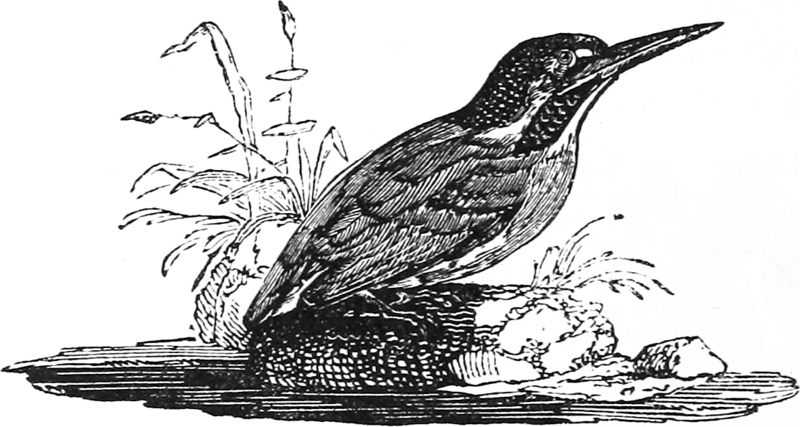
\includegraphics[scale=0.35]{images/Alycon.png}
        \end{figure}
        \vspace{0.5cm}
        \Huge
        \textbf{\textsc{Matematyka Dyskretna}}
        
        \vspace{0.5cm}
        \Large
        \textsc{Wybrane Dowody}
        
        \normalsize
        
        
        \line(1,0){330}
        
        \vspace{1cm}
        \textit{,,Myślę, że 7 punktów na 20 to nie jest zły wynik''}
        \vspace{1cm}

        \textit{\textsc{Popełnione przez}}\\
        \vspace{5mm}

        \textbf{\textsc{Dziurawy Ponton \\ Załatany Ponton \\ Puchaty Pompon \\ Zatopiony Ponton \\ Tonący Ponton \\ Notnop}}

        \vfill

        Kraków \\
        Anno Domini 2023
        
    \end{center}
    
\end{titlepage}


\tableofcontents
\section*{Licencja}
    \begin{figure}[h]
    	\begin{minipage}[c]{0.25\textwidth}
    		
\includegraphics[width=0.7\textwidth]{images/licencja.png}
    	\end{minipage}\hfill
    	\begin{minipage}[c]{0.75\textwidth}
    		\caption*{
    			Ten utwór jest dostępny na 
    			\href{https://creativecommons.org/licenses/by-sa/4.0/}{licencji Creative Commons Uznanie autorstwa
    			na tych samych warunkach 4.0 Międzynarodowe.}
    		}
    	\end{minipage}
    \end{figure}

% Actual content
\mainmatter

\chapter{Kombinatoryka}
 % Żeby nie było syfu to kolejne sekcje dodajemy do chapters/
% A potem includujemy za pomocą \input{chapters/...}

% Używamy \( \) i \[ \] zamiast dolarów -- tak jak się robi w LaTeXu


\documentclass[12pt, a4paper, polish, openany]{book}

% Please, let's familiarize ourselves with notatki.sty and tcs.sty so that we don't reinvent the wheel
\usepackage{notatki}

\fancyhead[L]{\textbf{\textit{MD}}}
\author{
}
\title{TCS and shitposting}


\begin{document}

% Front page and table of contents
\frontmatter

\input{titlepage}

\tableofcontents
\input{license}

% Actual content
\mainmatter

\chapter{Kombinatoryka}
\input{chapters/combinatorics/main}

\chapter{Zasada włączeń i wyłączeń}
\input{chapters/exclusion-inclusion/main}

\chapter{Posety}
\input{chapters/posets/main}

\chapter{Twierdzenie Ramseya}
\input{chapters/ramsey/main}

\chapter{Funkcje tworzące}
\input{chapters/generating_functions/main}

\chapter{Przepływy}
\input{chapters/flows/main}

\chapter{Skojarzenia}
\input{chapters/matchings/main}

\chapter{Kolorowanie grafów}
\input{chapters/graph-coloring/main}

\chapter{Grafy, ale nie kolorowanie}
\input{chapters/graph-misc/main}

\end{document}

\chapter{Zasada włączeń i wyłączeń}
 % Żeby nie było syfu to kolejne sekcje dodajemy do chapters/
% A potem includujemy za pomocą \input{chapters/...}

% Używamy \( \) i \[ \] zamiast dolarów -- tak jak się robi w LaTeXu


\documentclass[12pt, a4paper, polish, openany]{book}

% Please, let's familiarize ourselves with notatki.sty and tcs.sty so that we don't reinvent the wheel
\usepackage{notatki}

\fancyhead[L]{\textbf{\textit{MD}}}
\author{
}
\title{TCS and shitposting}


\begin{document}

% Front page and table of contents
\frontmatter

\input{titlepage}

\tableofcontents
\input{license}

% Actual content
\mainmatter

\chapter{Kombinatoryka}
\input{chapters/combinatorics/main}

\chapter{Zasada włączeń i wyłączeń}
\input{chapters/exclusion-inclusion/main}

\chapter{Posety}
\input{chapters/posets/main}

\chapter{Twierdzenie Ramseya}
\input{chapters/ramsey/main}

\chapter{Funkcje tworzące}
\input{chapters/generating_functions/main}

\chapter{Przepływy}
\input{chapters/flows/main}

\chapter{Skojarzenia}
\input{chapters/matchings/main}

\chapter{Kolorowanie grafów}
\input{chapters/graph-coloring/main}

\chapter{Grafy, ale nie kolorowanie}
\input{chapters/graph-misc/main}

\end{document}

\chapter{Posety}
 % Żeby nie było syfu to kolejne sekcje dodajemy do chapters/
% A potem includujemy za pomocą \input{chapters/...}

% Używamy \( \) i \[ \] zamiast dolarów -- tak jak się robi w LaTeXu


\documentclass[12pt, a4paper, polish, openany]{book}

% Please, let's familiarize ourselves with notatki.sty and tcs.sty so that we don't reinvent the wheel
\usepackage{notatki}

\fancyhead[L]{\textbf{\textit{MD}}}
\author{
}
\title{TCS and shitposting}


\begin{document}

% Front page and table of contents
\frontmatter

\input{titlepage}

\tableofcontents
\input{license}

% Actual content
\mainmatter

\chapter{Kombinatoryka}
\input{chapters/combinatorics/main}

\chapter{Zasada włączeń i wyłączeń}
\input{chapters/exclusion-inclusion/main}

\chapter{Posety}
\input{chapters/posets/main}

\chapter{Twierdzenie Ramseya}
\input{chapters/ramsey/main}

\chapter{Funkcje tworzące}
\input{chapters/generating_functions/main}

\chapter{Przepływy}
\input{chapters/flows/main}

\chapter{Skojarzenia}
\input{chapters/matchings/main}

\chapter{Kolorowanie grafów}
\input{chapters/graph-coloring/main}

\chapter{Grafy, ale nie kolorowanie}
\input{chapters/graph-misc/main}

\end{document}

\chapter{Twierdzenie Ramseya}
 % Żeby nie było syfu to kolejne sekcje dodajemy do chapters/
% A potem includujemy za pomocą \input{chapters/...}

% Używamy \( \) i \[ \] zamiast dolarów -- tak jak się robi w LaTeXu


\documentclass[12pt, a4paper, polish, openany]{book}

% Please, let's familiarize ourselves with notatki.sty and tcs.sty so that we don't reinvent the wheel
\usepackage{notatki}

\fancyhead[L]{\textbf{\textit{MD}}}
\author{
}
\title{TCS and shitposting}


\begin{document}

% Front page and table of contents
\frontmatter

\input{titlepage}

\tableofcontents
\input{license}

% Actual content
\mainmatter

\chapter{Kombinatoryka}
\input{chapters/combinatorics/main}

\chapter{Zasada włączeń i wyłączeń}
\input{chapters/exclusion-inclusion/main}

\chapter{Posety}
\input{chapters/posets/main}

\chapter{Twierdzenie Ramseya}
\input{chapters/ramsey/main}

\chapter{Funkcje tworzące}
\input{chapters/generating_functions/main}

\chapter{Przepływy}
\input{chapters/flows/main}

\chapter{Skojarzenia}
\input{chapters/matchings/main}

\chapter{Kolorowanie grafów}
\input{chapters/graph-coloring/main}

\chapter{Grafy, ale nie kolorowanie}
\input{chapters/graph-misc/main}

\end{document}

\chapter{Funkcje tworzące}
 % Żeby nie było syfu to kolejne sekcje dodajemy do chapters/
% A potem includujemy za pomocą \input{chapters/...}

% Używamy \( \) i \[ \] zamiast dolarów -- tak jak się robi w LaTeXu


\documentclass[12pt, a4paper, polish, openany]{book}

% Please, let's familiarize ourselves with notatki.sty and tcs.sty so that we don't reinvent the wheel
\usepackage{notatki}

\fancyhead[L]{\textbf{\textit{MD}}}
\author{
}
\title{TCS and shitposting}


\begin{document}

% Front page and table of contents
\frontmatter

\input{titlepage}

\tableofcontents
\input{license}

% Actual content
\mainmatter

\chapter{Kombinatoryka}
\input{chapters/combinatorics/main}

\chapter{Zasada włączeń i wyłączeń}
\input{chapters/exclusion-inclusion/main}

\chapter{Posety}
\input{chapters/posets/main}

\chapter{Twierdzenie Ramseya}
\input{chapters/ramsey/main}

\chapter{Funkcje tworzące}
\input{chapters/generating_functions/main}

\chapter{Przepływy}
\input{chapters/flows/main}

\chapter{Skojarzenia}
\input{chapters/matchings/main}

\chapter{Kolorowanie grafów}
\input{chapters/graph-coloring/main}

\chapter{Grafy, ale nie kolorowanie}
\input{chapters/graph-misc/main}

\end{document}

\chapter{Przepływy}
 % Żeby nie było syfu to kolejne sekcje dodajemy do chapters/
% A potem includujemy za pomocą \input{chapters/...}

% Używamy \( \) i \[ \] zamiast dolarów -- tak jak się robi w LaTeXu


\documentclass[12pt, a4paper, polish, openany]{book}

% Please, let's familiarize ourselves with notatki.sty and tcs.sty so that we don't reinvent the wheel
\usepackage{notatki}

\fancyhead[L]{\textbf{\textit{MD}}}
\author{
}
\title{TCS and shitposting}


\begin{document}

% Front page and table of contents
\frontmatter

\input{titlepage}

\tableofcontents
\input{license}

% Actual content
\mainmatter

\chapter{Kombinatoryka}
\input{chapters/combinatorics/main}

\chapter{Zasada włączeń i wyłączeń}
\input{chapters/exclusion-inclusion/main}

\chapter{Posety}
\input{chapters/posets/main}

\chapter{Twierdzenie Ramseya}
\input{chapters/ramsey/main}

\chapter{Funkcje tworzące}
\input{chapters/generating_functions/main}

\chapter{Przepływy}
\input{chapters/flows/main}

\chapter{Skojarzenia}
\input{chapters/matchings/main}

\chapter{Kolorowanie grafów}
\input{chapters/graph-coloring/main}

\chapter{Grafy, ale nie kolorowanie}
\input{chapters/graph-misc/main}

\end{document}

\chapter{Skojarzenia}
 % Żeby nie było syfu to kolejne sekcje dodajemy do chapters/
% A potem includujemy za pomocą \input{chapters/...}

% Używamy \( \) i \[ \] zamiast dolarów -- tak jak się robi w LaTeXu


\documentclass[12pt, a4paper, polish, openany]{book}

% Please, let's familiarize ourselves with notatki.sty and tcs.sty so that we don't reinvent the wheel
\usepackage{notatki}

\fancyhead[L]{\textbf{\textit{MD}}}
\author{
}
\title{TCS and shitposting}


\begin{document}

% Front page and table of contents
\frontmatter

\input{titlepage}

\tableofcontents
\input{license}

% Actual content
\mainmatter

\chapter{Kombinatoryka}
\input{chapters/combinatorics/main}

\chapter{Zasada włączeń i wyłączeń}
\input{chapters/exclusion-inclusion/main}

\chapter{Posety}
\input{chapters/posets/main}

\chapter{Twierdzenie Ramseya}
\input{chapters/ramsey/main}

\chapter{Funkcje tworzące}
\input{chapters/generating_functions/main}

\chapter{Przepływy}
\input{chapters/flows/main}

\chapter{Skojarzenia}
\input{chapters/matchings/main}

\chapter{Kolorowanie grafów}
\input{chapters/graph-coloring/main}

\chapter{Grafy, ale nie kolorowanie}
\input{chapters/graph-misc/main}

\end{document}

\chapter{Kolorowanie grafów}
 % Żeby nie było syfu to kolejne sekcje dodajemy do chapters/
% A potem includujemy za pomocą \input{chapters/...}

% Używamy \( \) i \[ \] zamiast dolarów -- tak jak się robi w LaTeXu


\documentclass[12pt, a4paper, polish, openany]{book}

% Please, let's familiarize ourselves with notatki.sty and tcs.sty so that we don't reinvent the wheel
\usepackage{notatki}

\fancyhead[L]{\textbf{\textit{MD}}}
\author{
}
\title{TCS and shitposting}


\begin{document}

% Front page and table of contents
\frontmatter

\input{titlepage}

\tableofcontents
\input{license}

% Actual content
\mainmatter

\chapter{Kombinatoryka}
\input{chapters/combinatorics/main}

\chapter{Zasada włączeń i wyłączeń}
\input{chapters/exclusion-inclusion/main}

\chapter{Posety}
\input{chapters/posets/main}

\chapter{Twierdzenie Ramseya}
\input{chapters/ramsey/main}

\chapter{Funkcje tworzące}
\input{chapters/generating_functions/main}

\chapter{Przepływy}
\input{chapters/flows/main}

\chapter{Skojarzenia}
\input{chapters/matchings/main}

\chapter{Kolorowanie grafów}
\input{chapters/graph-coloring/main}

\chapter{Grafy, ale nie kolorowanie}
\input{chapters/graph-misc/main}

\end{document}

\chapter{Grafy, ale nie kolorowanie}
 % Żeby nie było syfu to kolejne sekcje dodajemy do chapters/
% A potem includujemy za pomocą \input{chapters/...}

% Używamy \( \) i \[ \] zamiast dolarów -- tak jak się robi w LaTeXu


\documentclass[12pt, a4paper, polish, openany]{book}

% Please, let's familiarize ourselves with notatki.sty and tcs.sty so that we don't reinvent the wheel
\usepackage{notatki}

\fancyhead[L]{\textbf{\textit{MD}}}
\author{
}
\title{TCS and shitposting}


\begin{document}

% Front page and table of contents
\frontmatter

\input{titlepage}

\tableofcontents
\input{license}

% Actual content
\mainmatter

\chapter{Kombinatoryka}
\input{chapters/combinatorics/main}

\chapter{Zasada włączeń i wyłączeń}
\input{chapters/exclusion-inclusion/main}

\chapter{Posety}
\input{chapters/posets/main}

\chapter{Twierdzenie Ramseya}
\input{chapters/ramsey/main}

\chapter{Funkcje tworzące}
\input{chapters/generating_functions/main}

\chapter{Przepływy}
\input{chapters/flows/main}

\chapter{Skojarzenia}
\input{chapters/matchings/main}

\chapter{Kolorowanie grafów}
\input{chapters/graph-coloring/main}

\chapter{Grafy, ale nie kolorowanie}
\input{chapters/graph-misc/main}

\end{document}

\end{document}

\chapter{Przepływy}
 % Żeby nie było syfu to kolejne sekcje dodajemy do chapters/
% A potem includujemy za pomocą \input{chapters/...}

% Używamy \( \) i \[ \] zamiast dolarów -- tak jak się robi w LaTeXu


\documentclass[12pt, a4paper, polish, openany]{book}

% Please, let's familiarize ourselves with notatki.sty and tcs.sty so that we don't reinvent the wheel
\usepackage{notatki}

\fancyhead[L]{\textbf{\textit{MD}}}
\author{
}
\title{TCS and shitposting}


\begin{document}

% Front page and table of contents
\frontmatter

\begin{titlepage} 

    \begin{center}
         \begin{figure}[h]
            \centering
            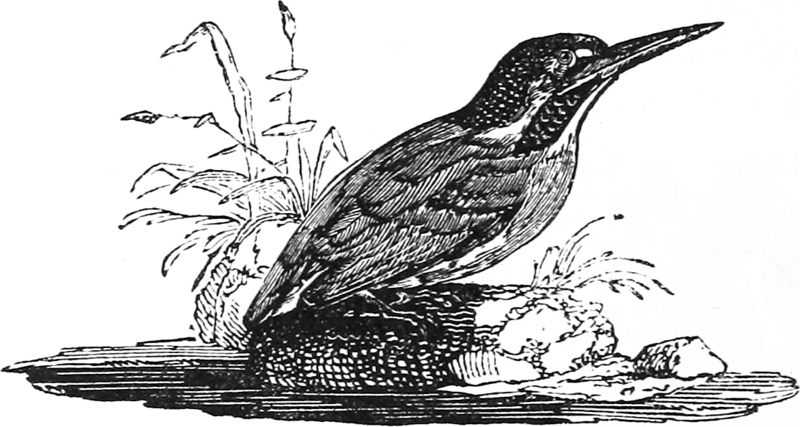
\includegraphics[scale=0.35]{images/Alycon.png}
        \end{figure}
        \vspace{0.5cm}
        \Huge
        \textbf{\textsc{Matematyka Dyskretna}}
        
        \vspace{0.5cm}
        \Large
        \textsc{Wybrane Dowody}
        
        \normalsize
        
        
        \line(1,0){330}
        
        \vspace{1cm}
        \textit{,,Myślę, że 7 punktów na 20 to nie jest zły wynik''}
        \vspace{1cm}

        \textit{\textsc{Popełnione przez}}\\
        \vspace{5mm}

        \textbf{\textsc{Dziurawy Ponton \\ Załatany Ponton \\ Puchaty Pompon \\ Zatopiony Ponton \\ Tonący Ponton \\ Notnop}}

        \vfill

        Kraków \\
        Anno Domini 2023
        
    \end{center}
    
\end{titlepage}


\tableofcontents
\section*{Licencja}
    \begin{figure}[h]
    	\begin{minipage}[c]{0.25\textwidth}
    		
\includegraphics[width=0.7\textwidth]{images/licencja.png}
    	\end{minipage}\hfill
    	\begin{minipage}[c]{0.75\textwidth}
    		\caption*{
    			Ten utwór jest dostępny na 
    			\href{https://creativecommons.org/licenses/by-sa/4.0/}{licencji Creative Commons Uznanie autorstwa
    			na tych samych warunkach 4.0 Międzynarodowe.}
    		}
    	\end{minipage}
    \end{figure}

% Actual content
\mainmatter

\chapter{Kombinatoryka}
 % Żeby nie było syfu to kolejne sekcje dodajemy do chapters/
% A potem includujemy za pomocą \input{chapters/...}

% Używamy \( \) i \[ \] zamiast dolarów -- tak jak się robi w LaTeXu


\documentclass[12pt, a4paper, polish, openany]{book}

% Please, let's familiarize ourselves with notatki.sty and tcs.sty so that we don't reinvent the wheel
\usepackage{notatki}

\fancyhead[L]{\textbf{\textit{MD}}}
\author{
}
\title{TCS and shitposting}


\begin{document}

% Front page and table of contents
\frontmatter

\input{titlepage}

\tableofcontents
\input{license}

% Actual content
\mainmatter

\chapter{Kombinatoryka}
\input{chapters/combinatorics/main}

\chapter{Zasada włączeń i wyłączeń}
\input{chapters/exclusion-inclusion/main}

\chapter{Posety}
\input{chapters/posets/main}

\chapter{Twierdzenie Ramseya}
\input{chapters/ramsey/main}

\chapter{Funkcje tworzące}
\input{chapters/generating_functions/main}

\chapter{Przepływy}
\input{chapters/flows/main}

\chapter{Skojarzenia}
\input{chapters/matchings/main}

\chapter{Kolorowanie grafów}
\input{chapters/graph-coloring/main}

\chapter{Grafy, ale nie kolorowanie}
\input{chapters/graph-misc/main}

\end{document}

\chapter{Zasada włączeń i wyłączeń}
 % Żeby nie było syfu to kolejne sekcje dodajemy do chapters/
% A potem includujemy za pomocą \input{chapters/...}

% Używamy \( \) i \[ \] zamiast dolarów -- tak jak się robi w LaTeXu


\documentclass[12pt, a4paper, polish, openany]{book}

% Please, let's familiarize ourselves with notatki.sty and tcs.sty so that we don't reinvent the wheel
\usepackage{notatki}

\fancyhead[L]{\textbf{\textit{MD}}}
\author{
}
\title{TCS and shitposting}


\begin{document}

% Front page and table of contents
\frontmatter

\input{titlepage}

\tableofcontents
\input{license}

% Actual content
\mainmatter

\chapter{Kombinatoryka}
\input{chapters/combinatorics/main}

\chapter{Zasada włączeń i wyłączeń}
\input{chapters/exclusion-inclusion/main}

\chapter{Posety}
\input{chapters/posets/main}

\chapter{Twierdzenie Ramseya}
\input{chapters/ramsey/main}

\chapter{Funkcje tworzące}
\input{chapters/generating_functions/main}

\chapter{Przepływy}
\input{chapters/flows/main}

\chapter{Skojarzenia}
\input{chapters/matchings/main}

\chapter{Kolorowanie grafów}
\input{chapters/graph-coloring/main}

\chapter{Grafy, ale nie kolorowanie}
\input{chapters/graph-misc/main}

\end{document}

\chapter{Posety}
 % Żeby nie było syfu to kolejne sekcje dodajemy do chapters/
% A potem includujemy za pomocą \input{chapters/...}

% Używamy \( \) i \[ \] zamiast dolarów -- tak jak się robi w LaTeXu


\documentclass[12pt, a4paper, polish, openany]{book}

% Please, let's familiarize ourselves with notatki.sty and tcs.sty so that we don't reinvent the wheel
\usepackage{notatki}

\fancyhead[L]{\textbf{\textit{MD}}}
\author{
}
\title{TCS and shitposting}


\begin{document}

% Front page and table of contents
\frontmatter

\input{titlepage}

\tableofcontents
\input{license}

% Actual content
\mainmatter

\chapter{Kombinatoryka}
\input{chapters/combinatorics/main}

\chapter{Zasada włączeń i wyłączeń}
\input{chapters/exclusion-inclusion/main}

\chapter{Posety}
\input{chapters/posets/main}

\chapter{Twierdzenie Ramseya}
\input{chapters/ramsey/main}

\chapter{Funkcje tworzące}
\input{chapters/generating_functions/main}

\chapter{Przepływy}
\input{chapters/flows/main}

\chapter{Skojarzenia}
\input{chapters/matchings/main}

\chapter{Kolorowanie grafów}
\input{chapters/graph-coloring/main}

\chapter{Grafy, ale nie kolorowanie}
\input{chapters/graph-misc/main}

\end{document}

\chapter{Twierdzenie Ramseya}
 % Żeby nie było syfu to kolejne sekcje dodajemy do chapters/
% A potem includujemy za pomocą \input{chapters/...}

% Używamy \( \) i \[ \] zamiast dolarów -- tak jak się robi w LaTeXu


\documentclass[12pt, a4paper, polish, openany]{book}

% Please, let's familiarize ourselves with notatki.sty and tcs.sty so that we don't reinvent the wheel
\usepackage{notatki}

\fancyhead[L]{\textbf{\textit{MD}}}
\author{
}
\title{TCS and shitposting}


\begin{document}

% Front page and table of contents
\frontmatter

\input{titlepage}

\tableofcontents
\input{license}

% Actual content
\mainmatter

\chapter{Kombinatoryka}
\input{chapters/combinatorics/main}

\chapter{Zasada włączeń i wyłączeń}
\input{chapters/exclusion-inclusion/main}

\chapter{Posety}
\input{chapters/posets/main}

\chapter{Twierdzenie Ramseya}
\input{chapters/ramsey/main}

\chapter{Funkcje tworzące}
\input{chapters/generating_functions/main}

\chapter{Przepływy}
\input{chapters/flows/main}

\chapter{Skojarzenia}
\input{chapters/matchings/main}

\chapter{Kolorowanie grafów}
\input{chapters/graph-coloring/main}

\chapter{Grafy, ale nie kolorowanie}
\input{chapters/graph-misc/main}

\end{document}

\chapter{Funkcje tworzące}
 % Żeby nie było syfu to kolejne sekcje dodajemy do chapters/
% A potem includujemy za pomocą \input{chapters/...}

% Używamy \( \) i \[ \] zamiast dolarów -- tak jak się robi w LaTeXu


\documentclass[12pt, a4paper, polish, openany]{book}

% Please, let's familiarize ourselves with notatki.sty and tcs.sty so that we don't reinvent the wheel
\usepackage{notatki}

\fancyhead[L]{\textbf{\textit{MD}}}
\author{
}
\title{TCS and shitposting}


\begin{document}

% Front page and table of contents
\frontmatter

\input{titlepage}

\tableofcontents
\input{license}

% Actual content
\mainmatter

\chapter{Kombinatoryka}
\input{chapters/combinatorics/main}

\chapter{Zasada włączeń i wyłączeń}
\input{chapters/exclusion-inclusion/main}

\chapter{Posety}
\input{chapters/posets/main}

\chapter{Twierdzenie Ramseya}
\input{chapters/ramsey/main}

\chapter{Funkcje tworzące}
\input{chapters/generating_functions/main}

\chapter{Przepływy}
\input{chapters/flows/main}

\chapter{Skojarzenia}
\input{chapters/matchings/main}

\chapter{Kolorowanie grafów}
\input{chapters/graph-coloring/main}

\chapter{Grafy, ale nie kolorowanie}
\input{chapters/graph-misc/main}

\end{document}

\chapter{Przepływy}
 % Żeby nie było syfu to kolejne sekcje dodajemy do chapters/
% A potem includujemy za pomocą \input{chapters/...}

% Używamy \( \) i \[ \] zamiast dolarów -- tak jak się robi w LaTeXu


\documentclass[12pt, a4paper, polish, openany]{book}

% Please, let's familiarize ourselves with notatki.sty and tcs.sty so that we don't reinvent the wheel
\usepackage{notatki}

\fancyhead[L]{\textbf{\textit{MD}}}
\author{
}
\title{TCS and shitposting}


\begin{document}

% Front page and table of contents
\frontmatter

\input{titlepage}

\tableofcontents
\input{license}

% Actual content
\mainmatter

\chapter{Kombinatoryka}
\input{chapters/combinatorics/main}

\chapter{Zasada włączeń i wyłączeń}
\input{chapters/exclusion-inclusion/main}

\chapter{Posety}
\input{chapters/posets/main}

\chapter{Twierdzenie Ramseya}
\input{chapters/ramsey/main}

\chapter{Funkcje tworzące}
\input{chapters/generating_functions/main}

\chapter{Przepływy}
\input{chapters/flows/main}

\chapter{Skojarzenia}
\input{chapters/matchings/main}

\chapter{Kolorowanie grafów}
\input{chapters/graph-coloring/main}

\chapter{Grafy, ale nie kolorowanie}
\input{chapters/graph-misc/main}

\end{document}

\chapter{Skojarzenia}
 % Żeby nie było syfu to kolejne sekcje dodajemy do chapters/
% A potem includujemy za pomocą \input{chapters/...}

% Używamy \( \) i \[ \] zamiast dolarów -- tak jak się robi w LaTeXu


\documentclass[12pt, a4paper, polish, openany]{book}

% Please, let's familiarize ourselves with notatki.sty and tcs.sty so that we don't reinvent the wheel
\usepackage{notatki}

\fancyhead[L]{\textbf{\textit{MD}}}
\author{
}
\title{TCS and shitposting}


\begin{document}

% Front page and table of contents
\frontmatter

\input{titlepage}

\tableofcontents
\input{license}

% Actual content
\mainmatter

\chapter{Kombinatoryka}
\input{chapters/combinatorics/main}

\chapter{Zasada włączeń i wyłączeń}
\input{chapters/exclusion-inclusion/main}

\chapter{Posety}
\input{chapters/posets/main}

\chapter{Twierdzenie Ramseya}
\input{chapters/ramsey/main}

\chapter{Funkcje tworzące}
\input{chapters/generating_functions/main}

\chapter{Przepływy}
\input{chapters/flows/main}

\chapter{Skojarzenia}
\input{chapters/matchings/main}

\chapter{Kolorowanie grafów}
\input{chapters/graph-coloring/main}

\chapter{Grafy, ale nie kolorowanie}
\input{chapters/graph-misc/main}

\end{document}

\chapter{Kolorowanie grafów}
 % Żeby nie było syfu to kolejne sekcje dodajemy do chapters/
% A potem includujemy za pomocą \input{chapters/...}

% Używamy \( \) i \[ \] zamiast dolarów -- tak jak się robi w LaTeXu


\documentclass[12pt, a4paper, polish, openany]{book}

% Please, let's familiarize ourselves with notatki.sty and tcs.sty so that we don't reinvent the wheel
\usepackage{notatki}

\fancyhead[L]{\textbf{\textit{MD}}}
\author{
}
\title{TCS and shitposting}


\begin{document}

% Front page and table of contents
\frontmatter

\input{titlepage}

\tableofcontents
\input{license}

% Actual content
\mainmatter

\chapter{Kombinatoryka}
\input{chapters/combinatorics/main}

\chapter{Zasada włączeń i wyłączeń}
\input{chapters/exclusion-inclusion/main}

\chapter{Posety}
\input{chapters/posets/main}

\chapter{Twierdzenie Ramseya}
\input{chapters/ramsey/main}

\chapter{Funkcje tworzące}
\input{chapters/generating_functions/main}

\chapter{Przepływy}
\input{chapters/flows/main}

\chapter{Skojarzenia}
\input{chapters/matchings/main}

\chapter{Kolorowanie grafów}
\input{chapters/graph-coloring/main}

\chapter{Grafy, ale nie kolorowanie}
\input{chapters/graph-misc/main}

\end{document}

\chapter{Grafy, ale nie kolorowanie}
 % Żeby nie było syfu to kolejne sekcje dodajemy do chapters/
% A potem includujemy za pomocą \input{chapters/...}

% Używamy \( \) i \[ \] zamiast dolarów -- tak jak się robi w LaTeXu


\documentclass[12pt, a4paper, polish, openany]{book}

% Please, let's familiarize ourselves with notatki.sty and tcs.sty so that we don't reinvent the wheel
\usepackage{notatki}

\fancyhead[L]{\textbf{\textit{MD}}}
\author{
}
\title{TCS and shitposting}


\begin{document}

% Front page and table of contents
\frontmatter

\input{titlepage}

\tableofcontents
\input{license}

% Actual content
\mainmatter

\chapter{Kombinatoryka}
\input{chapters/combinatorics/main}

\chapter{Zasada włączeń i wyłączeń}
\input{chapters/exclusion-inclusion/main}

\chapter{Posety}
\input{chapters/posets/main}

\chapter{Twierdzenie Ramseya}
\input{chapters/ramsey/main}

\chapter{Funkcje tworzące}
\input{chapters/generating_functions/main}

\chapter{Przepływy}
\input{chapters/flows/main}

\chapter{Skojarzenia}
\input{chapters/matchings/main}

\chapter{Kolorowanie grafów}
\input{chapters/graph-coloring/main}

\chapter{Grafy, ale nie kolorowanie}
\input{chapters/graph-misc/main}

\end{document}

\end{document}

\chapter{Skojarzenia}
 % Żeby nie było syfu to kolejne sekcje dodajemy do chapters/
% A potem includujemy za pomocą \input{chapters/...}

% Używamy \( \) i \[ \] zamiast dolarów -- tak jak się robi w LaTeXu


\documentclass[12pt, a4paper, polish, openany]{book}

% Please, let's familiarize ourselves with notatki.sty and tcs.sty so that we don't reinvent the wheel
\usepackage{notatki}

\fancyhead[L]{\textbf{\textit{MD}}}
\author{
}
\title{TCS and shitposting}


\begin{document}

% Front page and table of contents
\frontmatter

\begin{titlepage} 

    \begin{center}
         \begin{figure}[h]
            \centering
            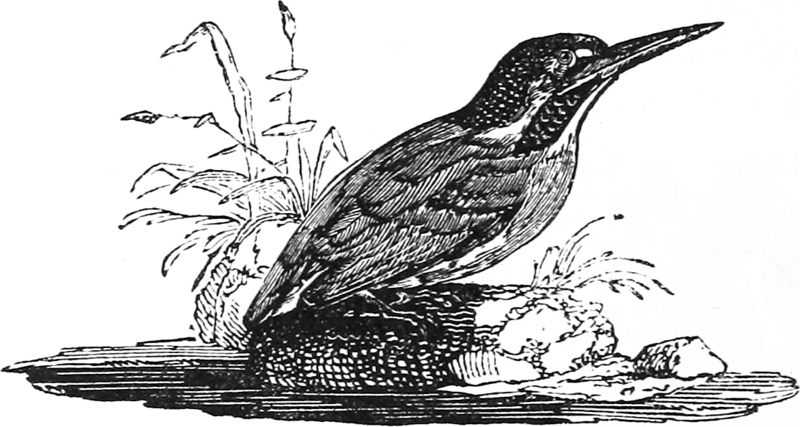
\includegraphics[scale=0.35]{images/Alycon.png}
        \end{figure}
        \vspace{0.5cm}
        \Huge
        \textbf{\textsc{Matematyka Dyskretna}}
        
        \vspace{0.5cm}
        \Large
        \textsc{Wybrane Dowody}
        
        \normalsize
        
        
        \line(1,0){330}
        
        \vspace{1cm}
        \textit{,,Myślę, że 7 punktów na 20 to nie jest zły wynik''}
        \vspace{1cm}

        \textit{\textsc{Popełnione przez}}\\
        \vspace{5mm}

        \textbf{\textsc{Dziurawy Ponton \\ Załatany Ponton \\ Puchaty Pompon \\ Zatopiony Ponton \\ Tonący Ponton \\ Notnop}}

        \vfill

        Kraków \\
        Anno Domini 2023
        
    \end{center}
    
\end{titlepage}


\tableofcontents
\section*{Licencja}
    \begin{figure}[h]
    	\begin{minipage}[c]{0.25\textwidth}
    		
\includegraphics[width=0.7\textwidth]{images/licencja.png}
    	\end{minipage}\hfill
    	\begin{minipage}[c]{0.75\textwidth}
    		\caption*{
    			Ten utwór jest dostępny na 
    			\href{https://creativecommons.org/licenses/by-sa/4.0/}{licencji Creative Commons Uznanie autorstwa
    			na tych samych warunkach 4.0 Międzynarodowe.}
    		}
    	\end{minipage}
    \end{figure}

% Actual content
\mainmatter

\chapter{Kombinatoryka}
 % Żeby nie było syfu to kolejne sekcje dodajemy do chapters/
% A potem includujemy za pomocą \input{chapters/...}

% Używamy \( \) i \[ \] zamiast dolarów -- tak jak się robi w LaTeXu


\documentclass[12pt, a4paper, polish, openany]{book}

% Please, let's familiarize ourselves with notatki.sty and tcs.sty so that we don't reinvent the wheel
\usepackage{notatki}

\fancyhead[L]{\textbf{\textit{MD}}}
\author{
}
\title{TCS and shitposting}


\begin{document}

% Front page and table of contents
\frontmatter

\input{titlepage}

\tableofcontents
\input{license}

% Actual content
\mainmatter

\chapter{Kombinatoryka}
\input{chapters/combinatorics/main}

\chapter{Zasada włączeń i wyłączeń}
\input{chapters/exclusion-inclusion/main}

\chapter{Posety}
\input{chapters/posets/main}

\chapter{Twierdzenie Ramseya}
\input{chapters/ramsey/main}

\chapter{Funkcje tworzące}
\input{chapters/generating_functions/main}

\chapter{Przepływy}
\input{chapters/flows/main}

\chapter{Skojarzenia}
\input{chapters/matchings/main}

\chapter{Kolorowanie grafów}
\input{chapters/graph-coloring/main}

\chapter{Grafy, ale nie kolorowanie}
\input{chapters/graph-misc/main}

\end{document}

\chapter{Zasada włączeń i wyłączeń}
 % Żeby nie było syfu to kolejne sekcje dodajemy do chapters/
% A potem includujemy za pomocą \input{chapters/...}

% Używamy \( \) i \[ \] zamiast dolarów -- tak jak się robi w LaTeXu


\documentclass[12pt, a4paper, polish, openany]{book}

% Please, let's familiarize ourselves with notatki.sty and tcs.sty so that we don't reinvent the wheel
\usepackage{notatki}

\fancyhead[L]{\textbf{\textit{MD}}}
\author{
}
\title{TCS and shitposting}


\begin{document}

% Front page and table of contents
\frontmatter

\input{titlepage}

\tableofcontents
\input{license}

% Actual content
\mainmatter

\chapter{Kombinatoryka}
\input{chapters/combinatorics/main}

\chapter{Zasada włączeń i wyłączeń}
\input{chapters/exclusion-inclusion/main}

\chapter{Posety}
\input{chapters/posets/main}

\chapter{Twierdzenie Ramseya}
\input{chapters/ramsey/main}

\chapter{Funkcje tworzące}
\input{chapters/generating_functions/main}

\chapter{Przepływy}
\input{chapters/flows/main}

\chapter{Skojarzenia}
\input{chapters/matchings/main}

\chapter{Kolorowanie grafów}
\input{chapters/graph-coloring/main}

\chapter{Grafy, ale nie kolorowanie}
\input{chapters/graph-misc/main}

\end{document}

\chapter{Posety}
 % Żeby nie było syfu to kolejne sekcje dodajemy do chapters/
% A potem includujemy za pomocą \input{chapters/...}

% Używamy \( \) i \[ \] zamiast dolarów -- tak jak się robi w LaTeXu


\documentclass[12pt, a4paper, polish, openany]{book}

% Please, let's familiarize ourselves with notatki.sty and tcs.sty so that we don't reinvent the wheel
\usepackage{notatki}

\fancyhead[L]{\textbf{\textit{MD}}}
\author{
}
\title{TCS and shitposting}


\begin{document}

% Front page and table of contents
\frontmatter

\input{titlepage}

\tableofcontents
\input{license}

% Actual content
\mainmatter

\chapter{Kombinatoryka}
\input{chapters/combinatorics/main}

\chapter{Zasada włączeń i wyłączeń}
\input{chapters/exclusion-inclusion/main}

\chapter{Posety}
\input{chapters/posets/main}

\chapter{Twierdzenie Ramseya}
\input{chapters/ramsey/main}

\chapter{Funkcje tworzące}
\input{chapters/generating_functions/main}

\chapter{Przepływy}
\input{chapters/flows/main}

\chapter{Skojarzenia}
\input{chapters/matchings/main}

\chapter{Kolorowanie grafów}
\input{chapters/graph-coloring/main}

\chapter{Grafy, ale nie kolorowanie}
\input{chapters/graph-misc/main}

\end{document}

\chapter{Twierdzenie Ramseya}
 % Żeby nie było syfu to kolejne sekcje dodajemy do chapters/
% A potem includujemy za pomocą \input{chapters/...}

% Używamy \( \) i \[ \] zamiast dolarów -- tak jak się robi w LaTeXu


\documentclass[12pt, a4paper, polish, openany]{book}

% Please, let's familiarize ourselves with notatki.sty and tcs.sty so that we don't reinvent the wheel
\usepackage{notatki}

\fancyhead[L]{\textbf{\textit{MD}}}
\author{
}
\title{TCS and shitposting}


\begin{document}

% Front page and table of contents
\frontmatter

\input{titlepage}

\tableofcontents
\input{license}

% Actual content
\mainmatter

\chapter{Kombinatoryka}
\input{chapters/combinatorics/main}

\chapter{Zasada włączeń i wyłączeń}
\input{chapters/exclusion-inclusion/main}

\chapter{Posety}
\input{chapters/posets/main}

\chapter{Twierdzenie Ramseya}
\input{chapters/ramsey/main}

\chapter{Funkcje tworzące}
\input{chapters/generating_functions/main}

\chapter{Przepływy}
\input{chapters/flows/main}

\chapter{Skojarzenia}
\input{chapters/matchings/main}

\chapter{Kolorowanie grafów}
\input{chapters/graph-coloring/main}

\chapter{Grafy, ale nie kolorowanie}
\input{chapters/graph-misc/main}

\end{document}

\chapter{Funkcje tworzące}
 % Żeby nie było syfu to kolejne sekcje dodajemy do chapters/
% A potem includujemy za pomocą \input{chapters/...}

% Używamy \( \) i \[ \] zamiast dolarów -- tak jak się robi w LaTeXu


\documentclass[12pt, a4paper, polish, openany]{book}

% Please, let's familiarize ourselves with notatki.sty and tcs.sty so that we don't reinvent the wheel
\usepackage{notatki}

\fancyhead[L]{\textbf{\textit{MD}}}
\author{
}
\title{TCS and shitposting}


\begin{document}

% Front page and table of contents
\frontmatter

\input{titlepage}

\tableofcontents
\input{license}

% Actual content
\mainmatter

\chapter{Kombinatoryka}
\input{chapters/combinatorics/main}

\chapter{Zasada włączeń i wyłączeń}
\input{chapters/exclusion-inclusion/main}

\chapter{Posety}
\input{chapters/posets/main}

\chapter{Twierdzenie Ramseya}
\input{chapters/ramsey/main}

\chapter{Funkcje tworzące}
\input{chapters/generating_functions/main}

\chapter{Przepływy}
\input{chapters/flows/main}

\chapter{Skojarzenia}
\input{chapters/matchings/main}

\chapter{Kolorowanie grafów}
\input{chapters/graph-coloring/main}

\chapter{Grafy, ale nie kolorowanie}
\input{chapters/graph-misc/main}

\end{document}

\chapter{Przepływy}
 % Żeby nie było syfu to kolejne sekcje dodajemy do chapters/
% A potem includujemy za pomocą \input{chapters/...}

% Używamy \( \) i \[ \] zamiast dolarów -- tak jak się robi w LaTeXu


\documentclass[12pt, a4paper, polish, openany]{book}

% Please, let's familiarize ourselves with notatki.sty and tcs.sty so that we don't reinvent the wheel
\usepackage{notatki}

\fancyhead[L]{\textbf{\textit{MD}}}
\author{
}
\title{TCS and shitposting}


\begin{document}

% Front page and table of contents
\frontmatter

\input{titlepage}

\tableofcontents
\input{license}

% Actual content
\mainmatter

\chapter{Kombinatoryka}
\input{chapters/combinatorics/main}

\chapter{Zasada włączeń i wyłączeń}
\input{chapters/exclusion-inclusion/main}

\chapter{Posety}
\input{chapters/posets/main}

\chapter{Twierdzenie Ramseya}
\input{chapters/ramsey/main}

\chapter{Funkcje tworzące}
\input{chapters/generating_functions/main}

\chapter{Przepływy}
\input{chapters/flows/main}

\chapter{Skojarzenia}
\input{chapters/matchings/main}

\chapter{Kolorowanie grafów}
\input{chapters/graph-coloring/main}

\chapter{Grafy, ale nie kolorowanie}
\input{chapters/graph-misc/main}

\end{document}

\chapter{Skojarzenia}
 % Żeby nie było syfu to kolejne sekcje dodajemy do chapters/
% A potem includujemy za pomocą \input{chapters/...}

% Używamy \( \) i \[ \] zamiast dolarów -- tak jak się robi w LaTeXu


\documentclass[12pt, a4paper, polish, openany]{book}

% Please, let's familiarize ourselves with notatki.sty and tcs.sty so that we don't reinvent the wheel
\usepackage{notatki}

\fancyhead[L]{\textbf{\textit{MD}}}
\author{
}
\title{TCS and shitposting}


\begin{document}

% Front page and table of contents
\frontmatter

\input{titlepage}

\tableofcontents
\input{license}

% Actual content
\mainmatter

\chapter{Kombinatoryka}
\input{chapters/combinatorics/main}

\chapter{Zasada włączeń i wyłączeń}
\input{chapters/exclusion-inclusion/main}

\chapter{Posety}
\input{chapters/posets/main}

\chapter{Twierdzenie Ramseya}
\input{chapters/ramsey/main}

\chapter{Funkcje tworzące}
\input{chapters/generating_functions/main}

\chapter{Przepływy}
\input{chapters/flows/main}

\chapter{Skojarzenia}
\input{chapters/matchings/main}

\chapter{Kolorowanie grafów}
\input{chapters/graph-coloring/main}

\chapter{Grafy, ale nie kolorowanie}
\input{chapters/graph-misc/main}

\end{document}

\chapter{Kolorowanie grafów}
 % Żeby nie było syfu to kolejne sekcje dodajemy do chapters/
% A potem includujemy za pomocą \input{chapters/...}

% Używamy \( \) i \[ \] zamiast dolarów -- tak jak się robi w LaTeXu


\documentclass[12pt, a4paper, polish, openany]{book}

% Please, let's familiarize ourselves with notatki.sty and tcs.sty so that we don't reinvent the wheel
\usepackage{notatki}

\fancyhead[L]{\textbf{\textit{MD}}}
\author{
}
\title{TCS and shitposting}


\begin{document}

% Front page and table of contents
\frontmatter

\input{titlepage}

\tableofcontents
\input{license}

% Actual content
\mainmatter

\chapter{Kombinatoryka}
\input{chapters/combinatorics/main}

\chapter{Zasada włączeń i wyłączeń}
\input{chapters/exclusion-inclusion/main}

\chapter{Posety}
\input{chapters/posets/main}

\chapter{Twierdzenie Ramseya}
\input{chapters/ramsey/main}

\chapter{Funkcje tworzące}
\input{chapters/generating_functions/main}

\chapter{Przepływy}
\input{chapters/flows/main}

\chapter{Skojarzenia}
\input{chapters/matchings/main}

\chapter{Kolorowanie grafów}
\input{chapters/graph-coloring/main}

\chapter{Grafy, ale nie kolorowanie}
\input{chapters/graph-misc/main}

\end{document}

\chapter{Grafy, ale nie kolorowanie}
 % Żeby nie było syfu to kolejne sekcje dodajemy do chapters/
% A potem includujemy za pomocą \input{chapters/...}

% Używamy \( \) i \[ \] zamiast dolarów -- tak jak się robi w LaTeXu


\documentclass[12pt, a4paper, polish, openany]{book}

% Please, let's familiarize ourselves with notatki.sty and tcs.sty so that we don't reinvent the wheel
\usepackage{notatki}

\fancyhead[L]{\textbf{\textit{MD}}}
\author{
}
\title{TCS and shitposting}


\begin{document}

% Front page and table of contents
\frontmatter

\input{titlepage}

\tableofcontents
\input{license}

% Actual content
\mainmatter

\chapter{Kombinatoryka}
\input{chapters/combinatorics/main}

\chapter{Zasada włączeń i wyłączeń}
\input{chapters/exclusion-inclusion/main}

\chapter{Posety}
\input{chapters/posets/main}

\chapter{Twierdzenie Ramseya}
\input{chapters/ramsey/main}

\chapter{Funkcje tworzące}
\input{chapters/generating_functions/main}

\chapter{Przepływy}
\input{chapters/flows/main}

\chapter{Skojarzenia}
\input{chapters/matchings/main}

\chapter{Kolorowanie grafów}
\input{chapters/graph-coloring/main}

\chapter{Grafy, ale nie kolorowanie}
\input{chapters/graph-misc/main}

\end{document}

\end{document}

\chapter{Kolorowanie grafów}
 % Żeby nie było syfu to kolejne sekcje dodajemy do chapters/
% A potem includujemy za pomocą \input{chapters/...}

% Używamy \( \) i \[ \] zamiast dolarów -- tak jak się robi w LaTeXu


\documentclass[12pt, a4paper, polish, openany]{book}

% Please, let's familiarize ourselves with notatki.sty and tcs.sty so that we don't reinvent the wheel
\usepackage{notatki}

\fancyhead[L]{\textbf{\textit{MD}}}
\author{
}
\title{TCS and shitposting}


\begin{document}

% Front page and table of contents
\frontmatter

\begin{titlepage} 

    \begin{center}
         \begin{figure}[h]
            \centering
            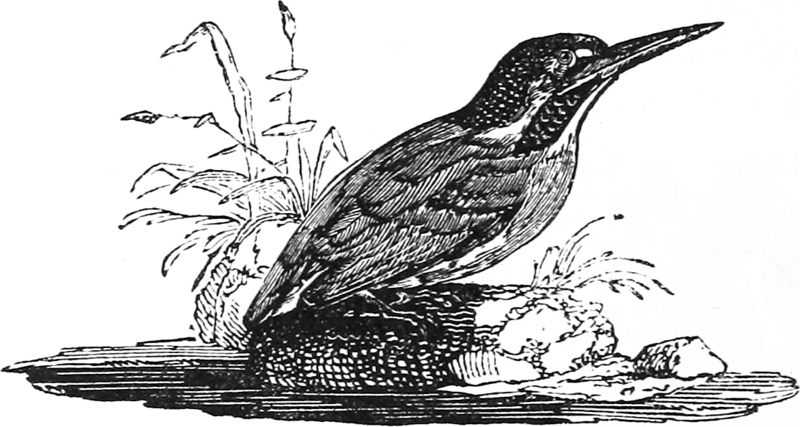
\includegraphics[scale=0.35]{images/Alycon.png}
        \end{figure}
        \vspace{0.5cm}
        \Huge
        \textbf{\textsc{Matematyka Dyskretna}}
        
        \vspace{0.5cm}
        \Large
        \textsc{Wybrane Dowody}
        
        \normalsize
        
        
        \line(1,0){330}
        
        \vspace{1cm}
        \textit{,,Myślę, że 7 punktów na 20 to nie jest zły wynik''}
        \vspace{1cm}

        \textit{\textsc{Popełnione przez}}\\
        \vspace{5mm}

        \textbf{\textsc{Dziurawy Ponton \\ Załatany Ponton \\ Puchaty Pompon \\ Zatopiony Ponton \\ Tonący Ponton \\ Notnop}}

        \vfill

        Kraków \\
        Anno Domini 2023
        
    \end{center}
    
\end{titlepage}


\tableofcontents
\section*{Licencja}
    \begin{figure}[h]
    	\begin{minipage}[c]{0.25\textwidth}
    		
\includegraphics[width=0.7\textwidth]{images/licencja.png}
    	\end{minipage}\hfill
    	\begin{minipage}[c]{0.75\textwidth}
    		\caption*{
    			Ten utwór jest dostępny na 
    			\href{https://creativecommons.org/licenses/by-sa/4.0/}{licencji Creative Commons Uznanie autorstwa
    			na tych samych warunkach 4.0 Międzynarodowe.}
    		}
    	\end{minipage}
    \end{figure}

% Actual content
\mainmatter

\chapter{Kombinatoryka}
 % Żeby nie było syfu to kolejne sekcje dodajemy do chapters/
% A potem includujemy za pomocą \input{chapters/...}

% Używamy \( \) i \[ \] zamiast dolarów -- tak jak się robi w LaTeXu


\documentclass[12pt, a4paper, polish, openany]{book}

% Please, let's familiarize ourselves with notatki.sty and tcs.sty so that we don't reinvent the wheel
\usepackage{notatki}

\fancyhead[L]{\textbf{\textit{MD}}}
\author{
}
\title{TCS and shitposting}


\begin{document}

% Front page and table of contents
\frontmatter

\input{titlepage}

\tableofcontents
\input{license}

% Actual content
\mainmatter

\chapter{Kombinatoryka}
\input{chapters/combinatorics/main}

\chapter{Zasada włączeń i wyłączeń}
\input{chapters/exclusion-inclusion/main}

\chapter{Posety}
\input{chapters/posets/main}

\chapter{Twierdzenie Ramseya}
\input{chapters/ramsey/main}

\chapter{Funkcje tworzące}
\input{chapters/generating_functions/main}

\chapter{Przepływy}
\input{chapters/flows/main}

\chapter{Skojarzenia}
\input{chapters/matchings/main}

\chapter{Kolorowanie grafów}
\input{chapters/graph-coloring/main}

\chapter{Grafy, ale nie kolorowanie}
\input{chapters/graph-misc/main}

\end{document}

\chapter{Zasada włączeń i wyłączeń}
 % Żeby nie było syfu to kolejne sekcje dodajemy do chapters/
% A potem includujemy za pomocą \input{chapters/...}

% Używamy \( \) i \[ \] zamiast dolarów -- tak jak się robi w LaTeXu


\documentclass[12pt, a4paper, polish, openany]{book}

% Please, let's familiarize ourselves with notatki.sty and tcs.sty so that we don't reinvent the wheel
\usepackage{notatki}

\fancyhead[L]{\textbf{\textit{MD}}}
\author{
}
\title{TCS and shitposting}


\begin{document}

% Front page and table of contents
\frontmatter

\input{titlepage}

\tableofcontents
\input{license}

% Actual content
\mainmatter

\chapter{Kombinatoryka}
\input{chapters/combinatorics/main}

\chapter{Zasada włączeń i wyłączeń}
\input{chapters/exclusion-inclusion/main}

\chapter{Posety}
\input{chapters/posets/main}

\chapter{Twierdzenie Ramseya}
\input{chapters/ramsey/main}

\chapter{Funkcje tworzące}
\input{chapters/generating_functions/main}

\chapter{Przepływy}
\input{chapters/flows/main}

\chapter{Skojarzenia}
\input{chapters/matchings/main}

\chapter{Kolorowanie grafów}
\input{chapters/graph-coloring/main}

\chapter{Grafy, ale nie kolorowanie}
\input{chapters/graph-misc/main}

\end{document}

\chapter{Posety}
 % Żeby nie było syfu to kolejne sekcje dodajemy do chapters/
% A potem includujemy za pomocą \input{chapters/...}

% Używamy \( \) i \[ \] zamiast dolarów -- tak jak się robi w LaTeXu


\documentclass[12pt, a4paper, polish, openany]{book}

% Please, let's familiarize ourselves with notatki.sty and tcs.sty so that we don't reinvent the wheel
\usepackage{notatki}

\fancyhead[L]{\textbf{\textit{MD}}}
\author{
}
\title{TCS and shitposting}


\begin{document}

% Front page and table of contents
\frontmatter

\input{titlepage}

\tableofcontents
\input{license}

% Actual content
\mainmatter

\chapter{Kombinatoryka}
\input{chapters/combinatorics/main}

\chapter{Zasada włączeń i wyłączeń}
\input{chapters/exclusion-inclusion/main}

\chapter{Posety}
\input{chapters/posets/main}

\chapter{Twierdzenie Ramseya}
\input{chapters/ramsey/main}

\chapter{Funkcje tworzące}
\input{chapters/generating_functions/main}

\chapter{Przepływy}
\input{chapters/flows/main}

\chapter{Skojarzenia}
\input{chapters/matchings/main}

\chapter{Kolorowanie grafów}
\input{chapters/graph-coloring/main}

\chapter{Grafy, ale nie kolorowanie}
\input{chapters/graph-misc/main}

\end{document}

\chapter{Twierdzenie Ramseya}
 % Żeby nie było syfu to kolejne sekcje dodajemy do chapters/
% A potem includujemy za pomocą \input{chapters/...}

% Używamy \( \) i \[ \] zamiast dolarów -- tak jak się robi w LaTeXu


\documentclass[12pt, a4paper, polish, openany]{book}

% Please, let's familiarize ourselves with notatki.sty and tcs.sty so that we don't reinvent the wheel
\usepackage{notatki}

\fancyhead[L]{\textbf{\textit{MD}}}
\author{
}
\title{TCS and shitposting}


\begin{document}

% Front page and table of contents
\frontmatter

\input{titlepage}

\tableofcontents
\input{license}

% Actual content
\mainmatter

\chapter{Kombinatoryka}
\input{chapters/combinatorics/main}

\chapter{Zasada włączeń i wyłączeń}
\input{chapters/exclusion-inclusion/main}

\chapter{Posety}
\input{chapters/posets/main}

\chapter{Twierdzenie Ramseya}
\input{chapters/ramsey/main}

\chapter{Funkcje tworzące}
\input{chapters/generating_functions/main}

\chapter{Przepływy}
\input{chapters/flows/main}

\chapter{Skojarzenia}
\input{chapters/matchings/main}

\chapter{Kolorowanie grafów}
\input{chapters/graph-coloring/main}

\chapter{Grafy, ale nie kolorowanie}
\input{chapters/graph-misc/main}

\end{document}

\chapter{Funkcje tworzące}
 % Żeby nie było syfu to kolejne sekcje dodajemy do chapters/
% A potem includujemy za pomocą \input{chapters/...}

% Używamy \( \) i \[ \] zamiast dolarów -- tak jak się robi w LaTeXu


\documentclass[12pt, a4paper, polish, openany]{book}

% Please, let's familiarize ourselves with notatki.sty and tcs.sty so that we don't reinvent the wheel
\usepackage{notatki}

\fancyhead[L]{\textbf{\textit{MD}}}
\author{
}
\title{TCS and shitposting}


\begin{document}

% Front page and table of contents
\frontmatter

\input{titlepage}

\tableofcontents
\input{license}

% Actual content
\mainmatter

\chapter{Kombinatoryka}
\input{chapters/combinatorics/main}

\chapter{Zasada włączeń i wyłączeń}
\input{chapters/exclusion-inclusion/main}

\chapter{Posety}
\input{chapters/posets/main}

\chapter{Twierdzenie Ramseya}
\input{chapters/ramsey/main}

\chapter{Funkcje tworzące}
\input{chapters/generating_functions/main}

\chapter{Przepływy}
\input{chapters/flows/main}

\chapter{Skojarzenia}
\input{chapters/matchings/main}

\chapter{Kolorowanie grafów}
\input{chapters/graph-coloring/main}

\chapter{Grafy, ale nie kolorowanie}
\input{chapters/graph-misc/main}

\end{document}

\chapter{Przepływy}
 % Żeby nie było syfu to kolejne sekcje dodajemy do chapters/
% A potem includujemy za pomocą \input{chapters/...}

% Używamy \( \) i \[ \] zamiast dolarów -- tak jak się robi w LaTeXu


\documentclass[12pt, a4paper, polish, openany]{book}

% Please, let's familiarize ourselves with notatki.sty and tcs.sty so that we don't reinvent the wheel
\usepackage{notatki}

\fancyhead[L]{\textbf{\textit{MD}}}
\author{
}
\title{TCS and shitposting}


\begin{document}

% Front page and table of contents
\frontmatter

\input{titlepage}

\tableofcontents
\input{license}

% Actual content
\mainmatter

\chapter{Kombinatoryka}
\input{chapters/combinatorics/main}

\chapter{Zasada włączeń i wyłączeń}
\input{chapters/exclusion-inclusion/main}

\chapter{Posety}
\input{chapters/posets/main}

\chapter{Twierdzenie Ramseya}
\input{chapters/ramsey/main}

\chapter{Funkcje tworzące}
\input{chapters/generating_functions/main}

\chapter{Przepływy}
\input{chapters/flows/main}

\chapter{Skojarzenia}
\input{chapters/matchings/main}

\chapter{Kolorowanie grafów}
\input{chapters/graph-coloring/main}

\chapter{Grafy, ale nie kolorowanie}
\input{chapters/graph-misc/main}

\end{document}

\chapter{Skojarzenia}
 % Żeby nie było syfu to kolejne sekcje dodajemy do chapters/
% A potem includujemy za pomocą \input{chapters/...}

% Używamy \( \) i \[ \] zamiast dolarów -- tak jak się robi w LaTeXu


\documentclass[12pt, a4paper, polish, openany]{book}

% Please, let's familiarize ourselves with notatki.sty and tcs.sty so that we don't reinvent the wheel
\usepackage{notatki}

\fancyhead[L]{\textbf{\textit{MD}}}
\author{
}
\title{TCS and shitposting}


\begin{document}

% Front page and table of contents
\frontmatter

\input{titlepage}

\tableofcontents
\input{license}

% Actual content
\mainmatter

\chapter{Kombinatoryka}
\input{chapters/combinatorics/main}

\chapter{Zasada włączeń i wyłączeń}
\input{chapters/exclusion-inclusion/main}

\chapter{Posety}
\input{chapters/posets/main}

\chapter{Twierdzenie Ramseya}
\input{chapters/ramsey/main}

\chapter{Funkcje tworzące}
\input{chapters/generating_functions/main}

\chapter{Przepływy}
\input{chapters/flows/main}

\chapter{Skojarzenia}
\input{chapters/matchings/main}

\chapter{Kolorowanie grafów}
\input{chapters/graph-coloring/main}

\chapter{Grafy, ale nie kolorowanie}
\input{chapters/graph-misc/main}

\end{document}

\chapter{Kolorowanie grafów}
 % Żeby nie było syfu to kolejne sekcje dodajemy do chapters/
% A potem includujemy za pomocą \input{chapters/...}

% Używamy \( \) i \[ \] zamiast dolarów -- tak jak się robi w LaTeXu


\documentclass[12pt, a4paper, polish, openany]{book}

% Please, let's familiarize ourselves with notatki.sty and tcs.sty so that we don't reinvent the wheel
\usepackage{notatki}

\fancyhead[L]{\textbf{\textit{MD}}}
\author{
}
\title{TCS and shitposting}


\begin{document}

% Front page and table of contents
\frontmatter

\input{titlepage}

\tableofcontents
\input{license}

% Actual content
\mainmatter

\chapter{Kombinatoryka}
\input{chapters/combinatorics/main}

\chapter{Zasada włączeń i wyłączeń}
\input{chapters/exclusion-inclusion/main}

\chapter{Posety}
\input{chapters/posets/main}

\chapter{Twierdzenie Ramseya}
\input{chapters/ramsey/main}

\chapter{Funkcje tworzące}
\input{chapters/generating_functions/main}

\chapter{Przepływy}
\input{chapters/flows/main}

\chapter{Skojarzenia}
\input{chapters/matchings/main}

\chapter{Kolorowanie grafów}
\input{chapters/graph-coloring/main}

\chapter{Grafy, ale nie kolorowanie}
\input{chapters/graph-misc/main}

\end{document}

\chapter{Grafy, ale nie kolorowanie}
 % Żeby nie było syfu to kolejne sekcje dodajemy do chapters/
% A potem includujemy za pomocą \input{chapters/...}

% Używamy \( \) i \[ \] zamiast dolarów -- tak jak się robi w LaTeXu


\documentclass[12pt, a4paper, polish, openany]{book}

% Please, let's familiarize ourselves with notatki.sty and tcs.sty so that we don't reinvent the wheel
\usepackage{notatki}

\fancyhead[L]{\textbf{\textit{MD}}}
\author{
}
\title{TCS and shitposting}


\begin{document}

% Front page and table of contents
\frontmatter

\input{titlepage}

\tableofcontents
\input{license}

% Actual content
\mainmatter

\chapter{Kombinatoryka}
\input{chapters/combinatorics/main}

\chapter{Zasada włączeń i wyłączeń}
\input{chapters/exclusion-inclusion/main}

\chapter{Posety}
\input{chapters/posets/main}

\chapter{Twierdzenie Ramseya}
\input{chapters/ramsey/main}

\chapter{Funkcje tworzące}
\input{chapters/generating_functions/main}

\chapter{Przepływy}
\input{chapters/flows/main}

\chapter{Skojarzenia}
\input{chapters/matchings/main}

\chapter{Kolorowanie grafów}
\input{chapters/graph-coloring/main}

\chapter{Grafy, ale nie kolorowanie}
\input{chapters/graph-misc/main}

\end{document}

\end{document}

\chapter{Grafy, ale nie kolorowanie}
 % Żeby nie było syfu to kolejne sekcje dodajemy do chapters/
% A potem includujemy za pomocą \input{chapters/...}

% Używamy \( \) i \[ \] zamiast dolarów -- tak jak się robi w LaTeXu


\documentclass[12pt, a4paper, polish, openany]{book}

% Please, let's familiarize ourselves with notatki.sty and tcs.sty so that we don't reinvent the wheel
\usepackage{notatki}

\fancyhead[L]{\textbf{\textit{MD}}}
\author{
}
\title{TCS and shitposting}


\begin{document}

% Front page and table of contents
\frontmatter

\begin{titlepage} 

    \begin{center}
         \begin{figure}[h]
            \centering
            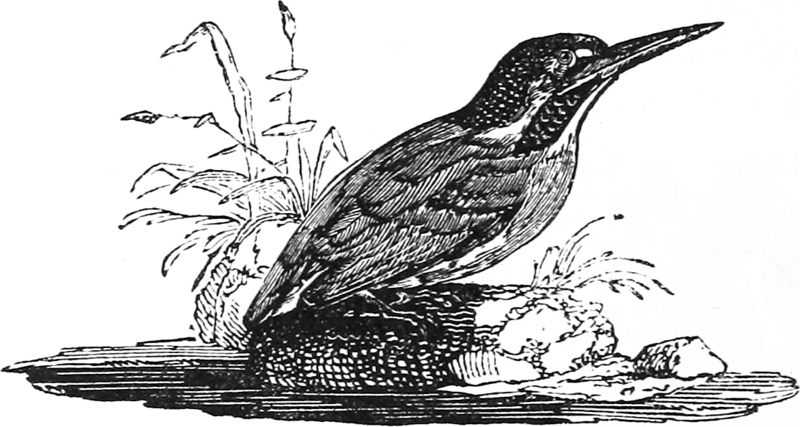
\includegraphics[scale=0.35]{images/Alycon.png}
        \end{figure}
        \vspace{0.5cm}
        \Huge
        \textbf{\textsc{Matematyka Dyskretna}}
        
        \vspace{0.5cm}
        \Large
        \textsc{Wybrane Dowody}
        
        \normalsize
        
        
        \line(1,0){330}
        
        \vspace{1cm}
        \textit{,,Myślę, że 7 punktów na 20 to nie jest zły wynik''}
        \vspace{1cm}

        \textit{\textsc{Popełnione przez}}\\
        \vspace{5mm}

        \textbf{\textsc{Dziurawy Ponton \\ Załatany Ponton \\ Puchaty Pompon \\ Zatopiony Ponton \\ Tonący Ponton \\ Notnop}}

        \vfill

        Kraków \\
        Anno Domini 2023
        
    \end{center}
    
\end{titlepage}


\tableofcontents
\section*{Licencja}
    \begin{figure}[h]
    	\begin{minipage}[c]{0.25\textwidth}
    		
\includegraphics[width=0.7\textwidth]{images/licencja.png}
    	\end{minipage}\hfill
    	\begin{minipage}[c]{0.75\textwidth}
    		\caption*{
    			Ten utwór jest dostępny na 
    			\href{https://creativecommons.org/licenses/by-sa/4.0/}{licencji Creative Commons Uznanie autorstwa
    			na tych samych warunkach 4.0 Międzynarodowe.}
    		}
    	\end{minipage}
    \end{figure}

% Actual content
\mainmatter

\chapter{Kombinatoryka}
 % Żeby nie było syfu to kolejne sekcje dodajemy do chapters/
% A potem includujemy za pomocą \input{chapters/...}

% Używamy \( \) i \[ \] zamiast dolarów -- tak jak się robi w LaTeXu


\documentclass[12pt, a4paper, polish, openany]{book}

% Please, let's familiarize ourselves with notatki.sty and tcs.sty so that we don't reinvent the wheel
\usepackage{notatki}

\fancyhead[L]{\textbf{\textit{MD}}}
\author{
}
\title{TCS and shitposting}


\begin{document}

% Front page and table of contents
\frontmatter

\input{titlepage}

\tableofcontents
\input{license}

% Actual content
\mainmatter

\chapter{Kombinatoryka}
\input{chapters/combinatorics/main}

\chapter{Zasada włączeń i wyłączeń}
\input{chapters/exclusion-inclusion/main}

\chapter{Posety}
\input{chapters/posets/main}

\chapter{Twierdzenie Ramseya}
\input{chapters/ramsey/main}

\chapter{Funkcje tworzące}
\input{chapters/generating_functions/main}

\chapter{Przepływy}
\input{chapters/flows/main}

\chapter{Skojarzenia}
\input{chapters/matchings/main}

\chapter{Kolorowanie grafów}
\input{chapters/graph-coloring/main}

\chapter{Grafy, ale nie kolorowanie}
\input{chapters/graph-misc/main}

\end{document}

\chapter{Zasada włączeń i wyłączeń}
 % Żeby nie było syfu to kolejne sekcje dodajemy do chapters/
% A potem includujemy za pomocą \input{chapters/...}

% Używamy \( \) i \[ \] zamiast dolarów -- tak jak się robi w LaTeXu


\documentclass[12pt, a4paper, polish, openany]{book}

% Please, let's familiarize ourselves with notatki.sty and tcs.sty so that we don't reinvent the wheel
\usepackage{notatki}

\fancyhead[L]{\textbf{\textit{MD}}}
\author{
}
\title{TCS and shitposting}


\begin{document}

% Front page and table of contents
\frontmatter

\input{titlepage}

\tableofcontents
\input{license}

% Actual content
\mainmatter

\chapter{Kombinatoryka}
\input{chapters/combinatorics/main}

\chapter{Zasada włączeń i wyłączeń}
\input{chapters/exclusion-inclusion/main}

\chapter{Posety}
\input{chapters/posets/main}

\chapter{Twierdzenie Ramseya}
\input{chapters/ramsey/main}

\chapter{Funkcje tworzące}
\input{chapters/generating_functions/main}

\chapter{Przepływy}
\input{chapters/flows/main}

\chapter{Skojarzenia}
\input{chapters/matchings/main}

\chapter{Kolorowanie grafów}
\input{chapters/graph-coloring/main}

\chapter{Grafy, ale nie kolorowanie}
\input{chapters/graph-misc/main}

\end{document}

\chapter{Posety}
 % Żeby nie było syfu to kolejne sekcje dodajemy do chapters/
% A potem includujemy za pomocą \input{chapters/...}

% Używamy \( \) i \[ \] zamiast dolarów -- tak jak się robi w LaTeXu


\documentclass[12pt, a4paper, polish, openany]{book}

% Please, let's familiarize ourselves with notatki.sty and tcs.sty so that we don't reinvent the wheel
\usepackage{notatki}

\fancyhead[L]{\textbf{\textit{MD}}}
\author{
}
\title{TCS and shitposting}


\begin{document}

% Front page and table of contents
\frontmatter

\input{titlepage}

\tableofcontents
\input{license}

% Actual content
\mainmatter

\chapter{Kombinatoryka}
\input{chapters/combinatorics/main}

\chapter{Zasada włączeń i wyłączeń}
\input{chapters/exclusion-inclusion/main}

\chapter{Posety}
\input{chapters/posets/main}

\chapter{Twierdzenie Ramseya}
\input{chapters/ramsey/main}

\chapter{Funkcje tworzące}
\input{chapters/generating_functions/main}

\chapter{Przepływy}
\input{chapters/flows/main}

\chapter{Skojarzenia}
\input{chapters/matchings/main}

\chapter{Kolorowanie grafów}
\input{chapters/graph-coloring/main}

\chapter{Grafy, ale nie kolorowanie}
\input{chapters/graph-misc/main}

\end{document}

\chapter{Twierdzenie Ramseya}
 % Żeby nie było syfu to kolejne sekcje dodajemy do chapters/
% A potem includujemy za pomocą \input{chapters/...}

% Używamy \( \) i \[ \] zamiast dolarów -- tak jak się robi w LaTeXu


\documentclass[12pt, a4paper, polish, openany]{book}

% Please, let's familiarize ourselves with notatki.sty and tcs.sty so that we don't reinvent the wheel
\usepackage{notatki}

\fancyhead[L]{\textbf{\textit{MD}}}
\author{
}
\title{TCS and shitposting}


\begin{document}

% Front page and table of contents
\frontmatter

\input{titlepage}

\tableofcontents
\input{license}

% Actual content
\mainmatter

\chapter{Kombinatoryka}
\input{chapters/combinatorics/main}

\chapter{Zasada włączeń i wyłączeń}
\input{chapters/exclusion-inclusion/main}

\chapter{Posety}
\input{chapters/posets/main}

\chapter{Twierdzenie Ramseya}
\input{chapters/ramsey/main}

\chapter{Funkcje tworzące}
\input{chapters/generating_functions/main}

\chapter{Przepływy}
\input{chapters/flows/main}

\chapter{Skojarzenia}
\input{chapters/matchings/main}

\chapter{Kolorowanie grafów}
\input{chapters/graph-coloring/main}

\chapter{Grafy, ale nie kolorowanie}
\input{chapters/graph-misc/main}

\end{document}

\chapter{Funkcje tworzące}
 % Żeby nie było syfu to kolejne sekcje dodajemy do chapters/
% A potem includujemy za pomocą \input{chapters/...}

% Używamy \( \) i \[ \] zamiast dolarów -- tak jak się robi w LaTeXu


\documentclass[12pt, a4paper, polish, openany]{book}

% Please, let's familiarize ourselves with notatki.sty and tcs.sty so that we don't reinvent the wheel
\usepackage{notatki}

\fancyhead[L]{\textbf{\textit{MD}}}
\author{
}
\title{TCS and shitposting}


\begin{document}

% Front page and table of contents
\frontmatter

\input{titlepage}

\tableofcontents
\input{license}

% Actual content
\mainmatter

\chapter{Kombinatoryka}
\input{chapters/combinatorics/main}

\chapter{Zasada włączeń i wyłączeń}
\input{chapters/exclusion-inclusion/main}

\chapter{Posety}
\input{chapters/posets/main}

\chapter{Twierdzenie Ramseya}
\input{chapters/ramsey/main}

\chapter{Funkcje tworzące}
\input{chapters/generating_functions/main}

\chapter{Przepływy}
\input{chapters/flows/main}

\chapter{Skojarzenia}
\input{chapters/matchings/main}

\chapter{Kolorowanie grafów}
\input{chapters/graph-coloring/main}

\chapter{Grafy, ale nie kolorowanie}
\input{chapters/graph-misc/main}

\end{document}

\chapter{Przepływy}
 % Żeby nie było syfu to kolejne sekcje dodajemy do chapters/
% A potem includujemy za pomocą \input{chapters/...}

% Używamy \( \) i \[ \] zamiast dolarów -- tak jak się robi w LaTeXu


\documentclass[12pt, a4paper, polish, openany]{book}

% Please, let's familiarize ourselves with notatki.sty and tcs.sty so that we don't reinvent the wheel
\usepackage{notatki}

\fancyhead[L]{\textbf{\textit{MD}}}
\author{
}
\title{TCS and shitposting}


\begin{document}

% Front page and table of contents
\frontmatter

\input{titlepage}

\tableofcontents
\input{license}

% Actual content
\mainmatter

\chapter{Kombinatoryka}
\input{chapters/combinatorics/main}

\chapter{Zasada włączeń i wyłączeń}
\input{chapters/exclusion-inclusion/main}

\chapter{Posety}
\input{chapters/posets/main}

\chapter{Twierdzenie Ramseya}
\input{chapters/ramsey/main}

\chapter{Funkcje tworzące}
\input{chapters/generating_functions/main}

\chapter{Przepływy}
\input{chapters/flows/main}

\chapter{Skojarzenia}
\input{chapters/matchings/main}

\chapter{Kolorowanie grafów}
\input{chapters/graph-coloring/main}

\chapter{Grafy, ale nie kolorowanie}
\input{chapters/graph-misc/main}

\end{document}

\chapter{Skojarzenia}
 % Żeby nie było syfu to kolejne sekcje dodajemy do chapters/
% A potem includujemy za pomocą \input{chapters/...}

% Używamy \( \) i \[ \] zamiast dolarów -- tak jak się robi w LaTeXu


\documentclass[12pt, a4paper, polish, openany]{book}

% Please, let's familiarize ourselves with notatki.sty and tcs.sty so that we don't reinvent the wheel
\usepackage{notatki}

\fancyhead[L]{\textbf{\textit{MD}}}
\author{
}
\title{TCS and shitposting}


\begin{document}

% Front page and table of contents
\frontmatter

\input{titlepage}

\tableofcontents
\input{license}

% Actual content
\mainmatter

\chapter{Kombinatoryka}
\input{chapters/combinatorics/main}

\chapter{Zasada włączeń i wyłączeń}
\input{chapters/exclusion-inclusion/main}

\chapter{Posety}
\input{chapters/posets/main}

\chapter{Twierdzenie Ramseya}
\input{chapters/ramsey/main}

\chapter{Funkcje tworzące}
\input{chapters/generating_functions/main}

\chapter{Przepływy}
\input{chapters/flows/main}

\chapter{Skojarzenia}
\input{chapters/matchings/main}

\chapter{Kolorowanie grafów}
\input{chapters/graph-coloring/main}

\chapter{Grafy, ale nie kolorowanie}
\input{chapters/graph-misc/main}

\end{document}

\chapter{Kolorowanie grafów}
 % Żeby nie było syfu to kolejne sekcje dodajemy do chapters/
% A potem includujemy za pomocą \input{chapters/...}

% Używamy \( \) i \[ \] zamiast dolarów -- tak jak się robi w LaTeXu


\documentclass[12pt, a4paper, polish, openany]{book}

% Please, let's familiarize ourselves with notatki.sty and tcs.sty so that we don't reinvent the wheel
\usepackage{notatki}

\fancyhead[L]{\textbf{\textit{MD}}}
\author{
}
\title{TCS and shitposting}


\begin{document}

% Front page and table of contents
\frontmatter

\input{titlepage}

\tableofcontents
\input{license}

% Actual content
\mainmatter

\chapter{Kombinatoryka}
\input{chapters/combinatorics/main}

\chapter{Zasada włączeń i wyłączeń}
\input{chapters/exclusion-inclusion/main}

\chapter{Posety}
\input{chapters/posets/main}

\chapter{Twierdzenie Ramseya}
\input{chapters/ramsey/main}

\chapter{Funkcje tworzące}
\input{chapters/generating_functions/main}

\chapter{Przepływy}
\input{chapters/flows/main}

\chapter{Skojarzenia}
\input{chapters/matchings/main}

\chapter{Kolorowanie grafów}
\input{chapters/graph-coloring/main}

\chapter{Grafy, ale nie kolorowanie}
\input{chapters/graph-misc/main}

\end{document}

\chapter{Grafy, ale nie kolorowanie}
 % Żeby nie było syfu to kolejne sekcje dodajemy do chapters/
% A potem includujemy za pomocą \input{chapters/...}

% Używamy \( \) i \[ \] zamiast dolarów -- tak jak się robi w LaTeXu


\documentclass[12pt, a4paper, polish, openany]{book}

% Please, let's familiarize ourselves with notatki.sty and tcs.sty so that we don't reinvent the wheel
\usepackage{notatki}

\fancyhead[L]{\textbf{\textit{MD}}}
\author{
}
\title{TCS and shitposting}


\begin{document}

% Front page and table of contents
\frontmatter

\input{titlepage}

\tableofcontents
\input{license}

% Actual content
\mainmatter

\chapter{Kombinatoryka}
\input{chapters/combinatorics/main}

\chapter{Zasada włączeń i wyłączeń}
\input{chapters/exclusion-inclusion/main}

\chapter{Posety}
\input{chapters/posets/main}

\chapter{Twierdzenie Ramseya}
\input{chapters/ramsey/main}

\chapter{Funkcje tworzące}
\input{chapters/generating_functions/main}

\chapter{Przepływy}
\input{chapters/flows/main}

\chapter{Skojarzenia}
\input{chapters/matchings/main}

\chapter{Kolorowanie grafów}
\input{chapters/graph-coloring/main}

\chapter{Grafy, ale nie kolorowanie}
\input{chapters/graph-misc/main}

\end{document}

\end{document}

\end{document}

\section{Domykanie relacji ze względu na różne własności. Podaj przykłady własności na które istnieje i~nie istnieje domknięcie}

\section{Zbiory przeliczalne i~ich przykłady}

\section{Konstrukcja Cantora liczb rzeczywistych. Porządek na liczbach rzeczywistych. Twierdzenie o~rozwinięciu liczby rzeczywistej w~szereg}

\section{Iloczyn kartezjański i~jego własności. Pojęcia relacji, złożenia, relacji odwrotnej, własności tych pojęć}
\label{mfi:cartesian_and_relations}
 % Żeby nie było syfu to kolejne sekcje dodajemy do chapters/
% A potem includujemy za pomocą \input{chapters/...}

% Używamy \( \) i \[ \] zamiast dolarów -- tak jak się robi w LaTeXu


\documentclass[12pt, a4paper, polish, openany]{book}

% Please, let's familiarize ourselves with notatki.sty and tcs.sty so that we don't reinvent the wheel
\usepackage{notatki}

\fancyhead[L]{\textbf{\textit{MD}}}
\author{
}
\title{TCS and shitposting}


\begin{document}

% Front page and table of contents
\frontmatter

\begin{titlepage} 

    \begin{center}
         \begin{figure}[h]
            \centering
            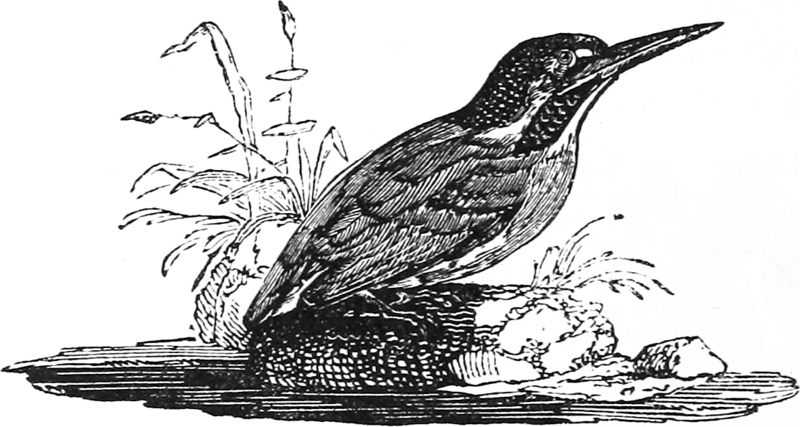
\includegraphics[scale=0.35]{images/Alycon.png}
        \end{figure}
        \vspace{0.5cm}
        \Huge
        \textbf{\textsc{Matematyka Dyskretna}}
        
        \vspace{0.5cm}
        \Large
        \textsc{Wybrane Dowody}
        
        \normalsize
        
        
        \line(1,0){330}
        
        \vspace{1cm}
        \textit{,,Myślę, że 7 punktów na 20 to nie jest zły wynik''}
        \vspace{1cm}

        \textit{\textsc{Popełnione przez}}\\
        \vspace{5mm}

        \textbf{\textsc{Dziurawy Ponton \\ Załatany Ponton \\ Puchaty Pompon \\ Zatopiony Ponton \\ Tonący Ponton \\ Notnop}}

        \vfill

        Kraków \\
        Anno Domini 2023
        
    \end{center}
    
\end{titlepage}


\tableofcontents
\section*{Licencja}
    \begin{figure}[h]
    	\begin{minipage}[c]{0.25\textwidth}
    		
\includegraphics[width=0.7\textwidth]{images/licencja.png}
    	\end{minipage}\hfill
    	\begin{minipage}[c]{0.75\textwidth}
    		\caption*{
    			Ten utwór jest dostępny na 
    			\href{https://creativecommons.org/licenses/by-sa/4.0/}{licencji Creative Commons Uznanie autorstwa
    			na tych samych warunkach 4.0 Międzynarodowe.}
    		}
    	\end{minipage}
    \end{figure}

% Actual content
\mainmatter

\chapter{Kombinatoryka}
 % Żeby nie było syfu to kolejne sekcje dodajemy do chapters/
% A potem includujemy za pomocą \input{chapters/...}

% Używamy \( \) i \[ \] zamiast dolarów -- tak jak się robi w LaTeXu


\documentclass[12pt, a4paper, polish, openany]{book}

% Please, let's familiarize ourselves with notatki.sty and tcs.sty so that we don't reinvent the wheel
\usepackage{notatki}

\fancyhead[L]{\textbf{\textit{MD}}}
\author{
}
\title{TCS and shitposting}


\begin{document}

% Front page and table of contents
\frontmatter

\begin{titlepage} 

    \begin{center}
         \begin{figure}[h]
            \centering
            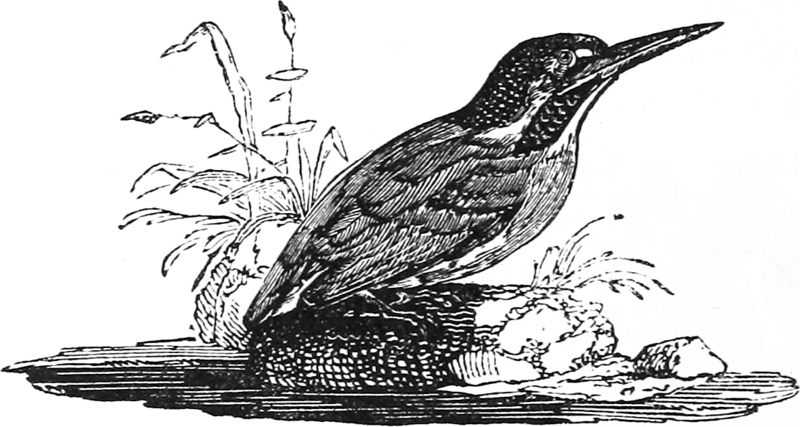
\includegraphics[scale=0.35]{images/Alycon.png}
        \end{figure}
        \vspace{0.5cm}
        \Huge
        \textbf{\textsc{Matematyka Dyskretna}}
        
        \vspace{0.5cm}
        \Large
        \textsc{Wybrane Dowody}
        
        \normalsize
        
        
        \line(1,0){330}
        
        \vspace{1cm}
        \textit{,,Myślę, że 7 punktów na 20 to nie jest zły wynik''}
        \vspace{1cm}

        \textit{\textsc{Popełnione przez}}\\
        \vspace{5mm}

        \textbf{\textsc{Dziurawy Ponton \\ Załatany Ponton \\ Puchaty Pompon \\ Zatopiony Ponton \\ Tonący Ponton \\ Notnop}}

        \vfill

        Kraków \\
        Anno Domini 2023
        
    \end{center}
    
\end{titlepage}


\tableofcontents
\section*{Licencja}
    \begin{figure}[h]
    	\begin{minipage}[c]{0.25\textwidth}
    		
\includegraphics[width=0.7\textwidth]{images/licencja.png}
    	\end{minipage}\hfill
    	\begin{minipage}[c]{0.75\textwidth}
    		\caption*{
    			Ten utwór jest dostępny na 
    			\href{https://creativecommons.org/licenses/by-sa/4.0/}{licencji Creative Commons Uznanie autorstwa
    			na tych samych warunkach 4.0 Międzynarodowe.}
    		}
    	\end{minipage}
    \end{figure}

% Actual content
\mainmatter

\chapter{Kombinatoryka}
 % Żeby nie było syfu to kolejne sekcje dodajemy do chapters/
% A potem includujemy za pomocą \input{chapters/...}

% Używamy \( \) i \[ \] zamiast dolarów -- tak jak się robi w LaTeXu


\documentclass[12pt, a4paper, polish, openany]{book}

% Please, let's familiarize ourselves with notatki.sty and tcs.sty so that we don't reinvent the wheel
\usepackage{notatki}

\fancyhead[L]{\textbf{\textit{MD}}}
\author{
}
\title{TCS and shitposting}


\begin{document}

% Front page and table of contents
\frontmatter

\input{titlepage}

\tableofcontents
\input{license}

% Actual content
\mainmatter

\chapter{Kombinatoryka}
\input{chapters/combinatorics/main}

\chapter{Zasada włączeń i wyłączeń}
\input{chapters/exclusion-inclusion/main}

\chapter{Posety}
\input{chapters/posets/main}

\chapter{Twierdzenie Ramseya}
\input{chapters/ramsey/main}

\chapter{Funkcje tworzące}
\input{chapters/generating_functions/main}

\chapter{Przepływy}
\input{chapters/flows/main}

\chapter{Skojarzenia}
\input{chapters/matchings/main}

\chapter{Kolorowanie grafów}
\input{chapters/graph-coloring/main}

\chapter{Grafy, ale nie kolorowanie}
\input{chapters/graph-misc/main}

\end{document}

\chapter{Zasada włączeń i wyłączeń}
 % Żeby nie było syfu to kolejne sekcje dodajemy do chapters/
% A potem includujemy za pomocą \input{chapters/...}

% Używamy \( \) i \[ \] zamiast dolarów -- tak jak się robi w LaTeXu


\documentclass[12pt, a4paper, polish, openany]{book}

% Please, let's familiarize ourselves with notatki.sty and tcs.sty so that we don't reinvent the wheel
\usepackage{notatki}

\fancyhead[L]{\textbf{\textit{MD}}}
\author{
}
\title{TCS and shitposting}


\begin{document}

% Front page and table of contents
\frontmatter

\input{titlepage}

\tableofcontents
\input{license}

% Actual content
\mainmatter

\chapter{Kombinatoryka}
\input{chapters/combinatorics/main}

\chapter{Zasada włączeń i wyłączeń}
\input{chapters/exclusion-inclusion/main}

\chapter{Posety}
\input{chapters/posets/main}

\chapter{Twierdzenie Ramseya}
\input{chapters/ramsey/main}

\chapter{Funkcje tworzące}
\input{chapters/generating_functions/main}

\chapter{Przepływy}
\input{chapters/flows/main}

\chapter{Skojarzenia}
\input{chapters/matchings/main}

\chapter{Kolorowanie grafów}
\input{chapters/graph-coloring/main}

\chapter{Grafy, ale nie kolorowanie}
\input{chapters/graph-misc/main}

\end{document}

\chapter{Posety}
 % Żeby nie było syfu to kolejne sekcje dodajemy do chapters/
% A potem includujemy za pomocą \input{chapters/...}

% Używamy \( \) i \[ \] zamiast dolarów -- tak jak się robi w LaTeXu


\documentclass[12pt, a4paper, polish, openany]{book}

% Please, let's familiarize ourselves with notatki.sty and tcs.sty so that we don't reinvent the wheel
\usepackage{notatki}

\fancyhead[L]{\textbf{\textit{MD}}}
\author{
}
\title{TCS and shitposting}


\begin{document}

% Front page and table of contents
\frontmatter

\input{titlepage}

\tableofcontents
\input{license}

% Actual content
\mainmatter

\chapter{Kombinatoryka}
\input{chapters/combinatorics/main}

\chapter{Zasada włączeń i wyłączeń}
\input{chapters/exclusion-inclusion/main}

\chapter{Posety}
\input{chapters/posets/main}

\chapter{Twierdzenie Ramseya}
\input{chapters/ramsey/main}

\chapter{Funkcje tworzące}
\input{chapters/generating_functions/main}

\chapter{Przepływy}
\input{chapters/flows/main}

\chapter{Skojarzenia}
\input{chapters/matchings/main}

\chapter{Kolorowanie grafów}
\input{chapters/graph-coloring/main}

\chapter{Grafy, ale nie kolorowanie}
\input{chapters/graph-misc/main}

\end{document}

\chapter{Twierdzenie Ramseya}
 % Żeby nie było syfu to kolejne sekcje dodajemy do chapters/
% A potem includujemy za pomocą \input{chapters/...}

% Używamy \( \) i \[ \] zamiast dolarów -- tak jak się robi w LaTeXu


\documentclass[12pt, a4paper, polish, openany]{book}

% Please, let's familiarize ourselves with notatki.sty and tcs.sty so that we don't reinvent the wheel
\usepackage{notatki}

\fancyhead[L]{\textbf{\textit{MD}}}
\author{
}
\title{TCS and shitposting}


\begin{document}

% Front page and table of contents
\frontmatter

\input{titlepage}

\tableofcontents
\input{license}

% Actual content
\mainmatter

\chapter{Kombinatoryka}
\input{chapters/combinatorics/main}

\chapter{Zasada włączeń i wyłączeń}
\input{chapters/exclusion-inclusion/main}

\chapter{Posety}
\input{chapters/posets/main}

\chapter{Twierdzenie Ramseya}
\input{chapters/ramsey/main}

\chapter{Funkcje tworzące}
\input{chapters/generating_functions/main}

\chapter{Przepływy}
\input{chapters/flows/main}

\chapter{Skojarzenia}
\input{chapters/matchings/main}

\chapter{Kolorowanie grafów}
\input{chapters/graph-coloring/main}

\chapter{Grafy, ale nie kolorowanie}
\input{chapters/graph-misc/main}

\end{document}

\chapter{Funkcje tworzące}
 % Żeby nie było syfu to kolejne sekcje dodajemy do chapters/
% A potem includujemy za pomocą \input{chapters/...}

% Używamy \( \) i \[ \] zamiast dolarów -- tak jak się robi w LaTeXu


\documentclass[12pt, a4paper, polish, openany]{book}

% Please, let's familiarize ourselves with notatki.sty and tcs.sty so that we don't reinvent the wheel
\usepackage{notatki}

\fancyhead[L]{\textbf{\textit{MD}}}
\author{
}
\title{TCS and shitposting}


\begin{document}

% Front page and table of contents
\frontmatter

\input{titlepage}

\tableofcontents
\input{license}

% Actual content
\mainmatter

\chapter{Kombinatoryka}
\input{chapters/combinatorics/main}

\chapter{Zasada włączeń i wyłączeń}
\input{chapters/exclusion-inclusion/main}

\chapter{Posety}
\input{chapters/posets/main}

\chapter{Twierdzenie Ramseya}
\input{chapters/ramsey/main}

\chapter{Funkcje tworzące}
\input{chapters/generating_functions/main}

\chapter{Przepływy}
\input{chapters/flows/main}

\chapter{Skojarzenia}
\input{chapters/matchings/main}

\chapter{Kolorowanie grafów}
\input{chapters/graph-coloring/main}

\chapter{Grafy, ale nie kolorowanie}
\input{chapters/graph-misc/main}

\end{document}

\chapter{Przepływy}
 % Żeby nie było syfu to kolejne sekcje dodajemy do chapters/
% A potem includujemy za pomocą \input{chapters/...}

% Używamy \( \) i \[ \] zamiast dolarów -- tak jak się robi w LaTeXu


\documentclass[12pt, a4paper, polish, openany]{book}

% Please, let's familiarize ourselves with notatki.sty and tcs.sty so that we don't reinvent the wheel
\usepackage{notatki}

\fancyhead[L]{\textbf{\textit{MD}}}
\author{
}
\title{TCS and shitposting}


\begin{document}

% Front page and table of contents
\frontmatter

\input{titlepage}

\tableofcontents
\input{license}

% Actual content
\mainmatter

\chapter{Kombinatoryka}
\input{chapters/combinatorics/main}

\chapter{Zasada włączeń i wyłączeń}
\input{chapters/exclusion-inclusion/main}

\chapter{Posety}
\input{chapters/posets/main}

\chapter{Twierdzenie Ramseya}
\input{chapters/ramsey/main}

\chapter{Funkcje tworzące}
\input{chapters/generating_functions/main}

\chapter{Przepływy}
\input{chapters/flows/main}

\chapter{Skojarzenia}
\input{chapters/matchings/main}

\chapter{Kolorowanie grafów}
\input{chapters/graph-coloring/main}

\chapter{Grafy, ale nie kolorowanie}
\input{chapters/graph-misc/main}

\end{document}

\chapter{Skojarzenia}
 % Żeby nie było syfu to kolejne sekcje dodajemy do chapters/
% A potem includujemy za pomocą \input{chapters/...}

% Używamy \( \) i \[ \] zamiast dolarów -- tak jak się robi w LaTeXu


\documentclass[12pt, a4paper, polish, openany]{book}

% Please, let's familiarize ourselves with notatki.sty and tcs.sty so that we don't reinvent the wheel
\usepackage{notatki}

\fancyhead[L]{\textbf{\textit{MD}}}
\author{
}
\title{TCS and shitposting}


\begin{document}

% Front page and table of contents
\frontmatter

\input{titlepage}

\tableofcontents
\input{license}

% Actual content
\mainmatter

\chapter{Kombinatoryka}
\input{chapters/combinatorics/main}

\chapter{Zasada włączeń i wyłączeń}
\input{chapters/exclusion-inclusion/main}

\chapter{Posety}
\input{chapters/posets/main}

\chapter{Twierdzenie Ramseya}
\input{chapters/ramsey/main}

\chapter{Funkcje tworzące}
\input{chapters/generating_functions/main}

\chapter{Przepływy}
\input{chapters/flows/main}

\chapter{Skojarzenia}
\input{chapters/matchings/main}

\chapter{Kolorowanie grafów}
\input{chapters/graph-coloring/main}

\chapter{Grafy, ale nie kolorowanie}
\input{chapters/graph-misc/main}

\end{document}

\chapter{Kolorowanie grafów}
 % Żeby nie było syfu to kolejne sekcje dodajemy do chapters/
% A potem includujemy za pomocą \input{chapters/...}

% Używamy \( \) i \[ \] zamiast dolarów -- tak jak się robi w LaTeXu


\documentclass[12pt, a4paper, polish, openany]{book}

% Please, let's familiarize ourselves with notatki.sty and tcs.sty so that we don't reinvent the wheel
\usepackage{notatki}

\fancyhead[L]{\textbf{\textit{MD}}}
\author{
}
\title{TCS and shitposting}


\begin{document}

% Front page and table of contents
\frontmatter

\input{titlepage}

\tableofcontents
\input{license}

% Actual content
\mainmatter

\chapter{Kombinatoryka}
\input{chapters/combinatorics/main}

\chapter{Zasada włączeń i wyłączeń}
\input{chapters/exclusion-inclusion/main}

\chapter{Posety}
\input{chapters/posets/main}

\chapter{Twierdzenie Ramseya}
\input{chapters/ramsey/main}

\chapter{Funkcje tworzące}
\input{chapters/generating_functions/main}

\chapter{Przepływy}
\input{chapters/flows/main}

\chapter{Skojarzenia}
\input{chapters/matchings/main}

\chapter{Kolorowanie grafów}
\input{chapters/graph-coloring/main}

\chapter{Grafy, ale nie kolorowanie}
\input{chapters/graph-misc/main}

\end{document}

\chapter{Grafy, ale nie kolorowanie}
 % Żeby nie było syfu to kolejne sekcje dodajemy do chapters/
% A potem includujemy za pomocą \input{chapters/...}

% Używamy \( \) i \[ \] zamiast dolarów -- tak jak się robi w LaTeXu


\documentclass[12pt, a4paper, polish, openany]{book}

% Please, let's familiarize ourselves with notatki.sty and tcs.sty so that we don't reinvent the wheel
\usepackage{notatki}

\fancyhead[L]{\textbf{\textit{MD}}}
\author{
}
\title{TCS and shitposting}


\begin{document}

% Front page and table of contents
\frontmatter

\input{titlepage}

\tableofcontents
\input{license}

% Actual content
\mainmatter

\chapter{Kombinatoryka}
\input{chapters/combinatorics/main}

\chapter{Zasada włączeń i wyłączeń}
\input{chapters/exclusion-inclusion/main}

\chapter{Posety}
\input{chapters/posets/main}

\chapter{Twierdzenie Ramseya}
\input{chapters/ramsey/main}

\chapter{Funkcje tworzące}
\input{chapters/generating_functions/main}

\chapter{Przepływy}
\input{chapters/flows/main}

\chapter{Skojarzenia}
\input{chapters/matchings/main}

\chapter{Kolorowanie grafów}
\input{chapters/graph-coloring/main}

\chapter{Grafy, ale nie kolorowanie}
\input{chapters/graph-misc/main}

\end{document}

\end{document}

\chapter{Zasada włączeń i wyłączeń}
 % Żeby nie było syfu to kolejne sekcje dodajemy do chapters/
% A potem includujemy za pomocą \input{chapters/...}

% Używamy \( \) i \[ \] zamiast dolarów -- tak jak się robi w LaTeXu


\documentclass[12pt, a4paper, polish, openany]{book}

% Please, let's familiarize ourselves with notatki.sty and tcs.sty so that we don't reinvent the wheel
\usepackage{notatki}

\fancyhead[L]{\textbf{\textit{MD}}}
\author{
}
\title{TCS and shitposting}


\begin{document}

% Front page and table of contents
\frontmatter

\begin{titlepage} 

    \begin{center}
         \begin{figure}[h]
            \centering
            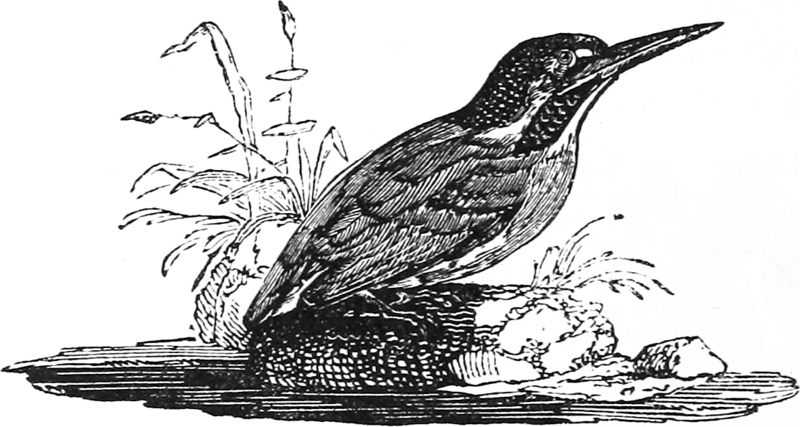
\includegraphics[scale=0.35]{images/Alycon.png}
        \end{figure}
        \vspace{0.5cm}
        \Huge
        \textbf{\textsc{Matematyka Dyskretna}}
        
        \vspace{0.5cm}
        \Large
        \textsc{Wybrane Dowody}
        
        \normalsize
        
        
        \line(1,0){330}
        
        \vspace{1cm}
        \textit{,,Myślę, że 7 punktów na 20 to nie jest zły wynik''}
        \vspace{1cm}

        \textit{\textsc{Popełnione przez}}\\
        \vspace{5mm}

        \textbf{\textsc{Dziurawy Ponton \\ Załatany Ponton \\ Puchaty Pompon \\ Zatopiony Ponton \\ Tonący Ponton \\ Notnop}}

        \vfill

        Kraków \\
        Anno Domini 2023
        
    \end{center}
    
\end{titlepage}


\tableofcontents
\section*{Licencja}
    \begin{figure}[h]
    	\begin{minipage}[c]{0.25\textwidth}
    		
\includegraphics[width=0.7\textwidth]{images/licencja.png}
    	\end{minipage}\hfill
    	\begin{minipage}[c]{0.75\textwidth}
    		\caption*{
    			Ten utwór jest dostępny na 
    			\href{https://creativecommons.org/licenses/by-sa/4.0/}{licencji Creative Commons Uznanie autorstwa
    			na tych samych warunkach 4.0 Międzynarodowe.}
    		}
    	\end{minipage}
    \end{figure}

% Actual content
\mainmatter

\chapter{Kombinatoryka}
 % Żeby nie było syfu to kolejne sekcje dodajemy do chapters/
% A potem includujemy za pomocą \input{chapters/...}

% Używamy \( \) i \[ \] zamiast dolarów -- tak jak się robi w LaTeXu


\documentclass[12pt, a4paper, polish, openany]{book}

% Please, let's familiarize ourselves with notatki.sty and tcs.sty so that we don't reinvent the wheel
\usepackage{notatki}

\fancyhead[L]{\textbf{\textit{MD}}}
\author{
}
\title{TCS and shitposting}


\begin{document}

% Front page and table of contents
\frontmatter

\input{titlepage}

\tableofcontents
\input{license}

% Actual content
\mainmatter

\chapter{Kombinatoryka}
\input{chapters/combinatorics/main}

\chapter{Zasada włączeń i wyłączeń}
\input{chapters/exclusion-inclusion/main}

\chapter{Posety}
\input{chapters/posets/main}

\chapter{Twierdzenie Ramseya}
\input{chapters/ramsey/main}

\chapter{Funkcje tworzące}
\input{chapters/generating_functions/main}

\chapter{Przepływy}
\input{chapters/flows/main}

\chapter{Skojarzenia}
\input{chapters/matchings/main}

\chapter{Kolorowanie grafów}
\input{chapters/graph-coloring/main}

\chapter{Grafy, ale nie kolorowanie}
\input{chapters/graph-misc/main}

\end{document}

\chapter{Zasada włączeń i wyłączeń}
 % Żeby nie było syfu to kolejne sekcje dodajemy do chapters/
% A potem includujemy za pomocą \input{chapters/...}

% Używamy \( \) i \[ \] zamiast dolarów -- tak jak się robi w LaTeXu


\documentclass[12pt, a4paper, polish, openany]{book}

% Please, let's familiarize ourselves with notatki.sty and tcs.sty so that we don't reinvent the wheel
\usepackage{notatki}

\fancyhead[L]{\textbf{\textit{MD}}}
\author{
}
\title{TCS and shitposting}


\begin{document}

% Front page and table of contents
\frontmatter

\input{titlepage}

\tableofcontents
\input{license}

% Actual content
\mainmatter

\chapter{Kombinatoryka}
\input{chapters/combinatorics/main}

\chapter{Zasada włączeń i wyłączeń}
\input{chapters/exclusion-inclusion/main}

\chapter{Posety}
\input{chapters/posets/main}

\chapter{Twierdzenie Ramseya}
\input{chapters/ramsey/main}

\chapter{Funkcje tworzące}
\input{chapters/generating_functions/main}

\chapter{Przepływy}
\input{chapters/flows/main}

\chapter{Skojarzenia}
\input{chapters/matchings/main}

\chapter{Kolorowanie grafów}
\input{chapters/graph-coloring/main}

\chapter{Grafy, ale nie kolorowanie}
\input{chapters/graph-misc/main}

\end{document}

\chapter{Posety}
 % Żeby nie było syfu to kolejne sekcje dodajemy do chapters/
% A potem includujemy za pomocą \input{chapters/...}

% Używamy \( \) i \[ \] zamiast dolarów -- tak jak się robi w LaTeXu


\documentclass[12pt, a4paper, polish, openany]{book}

% Please, let's familiarize ourselves with notatki.sty and tcs.sty so that we don't reinvent the wheel
\usepackage{notatki}

\fancyhead[L]{\textbf{\textit{MD}}}
\author{
}
\title{TCS and shitposting}


\begin{document}

% Front page and table of contents
\frontmatter

\input{titlepage}

\tableofcontents
\input{license}

% Actual content
\mainmatter

\chapter{Kombinatoryka}
\input{chapters/combinatorics/main}

\chapter{Zasada włączeń i wyłączeń}
\input{chapters/exclusion-inclusion/main}

\chapter{Posety}
\input{chapters/posets/main}

\chapter{Twierdzenie Ramseya}
\input{chapters/ramsey/main}

\chapter{Funkcje tworzące}
\input{chapters/generating_functions/main}

\chapter{Przepływy}
\input{chapters/flows/main}

\chapter{Skojarzenia}
\input{chapters/matchings/main}

\chapter{Kolorowanie grafów}
\input{chapters/graph-coloring/main}

\chapter{Grafy, ale nie kolorowanie}
\input{chapters/graph-misc/main}

\end{document}

\chapter{Twierdzenie Ramseya}
 % Żeby nie było syfu to kolejne sekcje dodajemy do chapters/
% A potem includujemy za pomocą \input{chapters/...}

% Używamy \( \) i \[ \] zamiast dolarów -- tak jak się robi w LaTeXu


\documentclass[12pt, a4paper, polish, openany]{book}

% Please, let's familiarize ourselves with notatki.sty and tcs.sty so that we don't reinvent the wheel
\usepackage{notatki}

\fancyhead[L]{\textbf{\textit{MD}}}
\author{
}
\title{TCS and shitposting}


\begin{document}

% Front page and table of contents
\frontmatter

\input{titlepage}

\tableofcontents
\input{license}

% Actual content
\mainmatter

\chapter{Kombinatoryka}
\input{chapters/combinatorics/main}

\chapter{Zasada włączeń i wyłączeń}
\input{chapters/exclusion-inclusion/main}

\chapter{Posety}
\input{chapters/posets/main}

\chapter{Twierdzenie Ramseya}
\input{chapters/ramsey/main}

\chapter{Funkcje tworzące}
\input{chapters/generating_functions/main}

\chapter{Przepływy}
\input{chapters/flows/main}

\chapter{Skojarzenia}
\input{chapters/matchings/main}

\chapter{Kolorowanie grafów}
\input{chapters/graph-coloring/main}

\chapter{Grafy, ale nie kolorowanie}
\input{chapters/graph-misc/main}

\end{document}

\chapter{Funkcje tworzące}
 % Żeby nie było syfu to kolejne sekcje dodajemy do chapters/
% A potem includujemy za pomocą \input{chapters/...}

% Używamy \( \) i \[ \] zamiast dolarów -- tak jak się robi w LaTeXu


\documentclass[12pt, a4paper, polish, openany]{book}

% Please, let's familiarize ourselves with notatki.sty and tcs.sty so that we don't reinvent the wheel
\usepackage{notatki}

\fancyhead[L]{\textbf{\textit{MD}}}
\author{
}
\title{TCS and shitposting}


\begin{document}

% Front page and table of contents
\frontmatter

\input{titlepage}

\tableofcontents
\input{license}

% Actual content
\mainmatter

\chapter{Kombinatoryka}
\input{chapters/combinatorics/main}

\chapter{Zasada włączeń i wyłączeń}
\input{chapters/exclusion-inclusion/main}

\chapter{Posety}
\input{chapters/posets/main}

\chapter{Twierdzenie Ramseya}
\input{chapters/ramsey/main}

\chapter{Funkcje tworzące}
\input{chapters/generating_functions/main}

\chapter{Przepływy}
\input{chapters/flows/main}

\chapter{Skojarzenia}
\input{chapters/matchings/main}

\chapter{Kolorowanie grafów}
\input{chapters/graph-coloring/main}

\chapter{Grafy, ale nie kolorowanie}
\input{chapters/graph-misc/main}

\end{document}

\chapter{Przepływy}
 % Żeby nie było syfu to kolejne sekcje dodajemy do chapters/
% A potem includujemy za pomocą \input{chapters/...}

% Używamy \( \) i \[ \] zamiast dolarów -- tak jak się robi w LaTeXu


\documentclass[12pt, a4paper, polish, openany]{book}

% Please, let's familiarize ourselves with notatki.sty and tcs.sty so that we don't reinvent the wheel
\usepackage{notatki}

\fancyhead[L]{\textbf{\textit{MD}}}
\author{
}
\title{TCS and shitposting}


\begin{document}

% Front page and table of contents
\frontmatter

\input{titlepage}

\tableofcontents
\input{license}

% Actual content
\mainmatter

\chapter{Kombinatoryka}
\input{chapters/combinatorics/main}

\chapter{Zasada włączeń i wyłączeń}
\input{chapters/exclusion-inclusion/main}

\chapter{Posety}
\input{chapters/posets/main}

\chapter{Twierdzenie Ramseya}
\input{chapters/ramsey/main}

\chapter{Funkcje tworzące}
\input{chapters/generating_functions/main}

\chapter{Przepływy}
\input{chapters/flows/main}

\chapter{Skojarzenia}
\input{chapters/matchings/main}

\chapter{Kolorowanie grafów}
\input{chapters/graph-coloring/main}

\chapter{Grafy, ale nie kolorowanie}
\input{chapters/graph-misc/main}

\end{document}

\chapter{Skojarzenia}
 % Żeby nie było syfu to kolejne sekcje dodajemy do chapters/
% A potem includujemy za pomocą \input{chapters/...}

% Używamy \( \) i \[ \] zamiast dolarów -- tak jak się robi w LaTeXu


\documentclass[12pt, a4paper, polish, openany]{book}

% Please, let's familiarize ourselves with notatki.sty and tcs.sty so that we don't reinvent the wheel
\usepackage{notatki}

\fancyhead[L]{\textbf{\textit{MD}}}
\author{
}
\title{TCS and shitposting}


\begin{document}

% Front page and table of contents
\frontmatter

\input{titlepage}

\tableofcontents
\input{license}

% Actual content
\mainmatter

\chapter{Kombinatoryka}
\input{chapters/combinatorics/main}

\chapter{Zasada włączeń i wyłączeń}
\input{chapters/exclusion-inclusion/main}

\chapter{Posety}
\input{chapters/posets/main}

\chapter{Twierdzenie Ramseya}
\input{chapters/ramsey/main}

\chapter{Funkcje tworzące}
\input{chapters/generating_functions/main}

\chapter{Przepływy}
\input{chapters/flows/main}

\chapter{Skojarzenia}
\input{chapters/matchings/main}

\chapter{Kolorowanie grafów}
\input{chapters/graph-coloring/main}

\chapter{Grafy, ale nie kolorowanie}
\input{chapters/graph-misc/main}

\end{document}

\chapter{Kolorowanie grafów}
 % Żeby nie było syfu to kolejne sekcje dodajemy do chapters/
% A potem includujemy za pomocą \input{chapters/...}

% Używamy \( \) i \[ \] zamiast dolarów -- tak jak się robi w LaTeXu


\documentclass[12pt, a4paper, polish, openany]{book}

% Please, let's familiarize ourselves with notatki.sty and tcs.sty so that we don't reinvent the wheel
\usepackage{notatki}

\fancyhead[L]{\textbf{\textit{MD}}}
\author{
}
\title{TCS and shitposting}


\begin{document}

% Front page and table of contents
\frontmatter

\input{titlepage}

\tableofcontents
\input{license}

% Actual content
\mainmatter

\chapter{Kombinatoryka}
\input{chapters/combinatorics/main}

\chapter{Zasada włączeń i wyłączeń}
\input{chapters/exclusion-inclusion/main}

\chapter{Posety}
\input{chapters/posets/main}

\chapter{Twierdzenie Ramseya}
\input{chapters/ramsey/main}

\chapter{Funkcje tworzące}
\input{chapters/generating_functions/main}

\chapter{Przepływy}
\input{chapters/flows/main}

\chapter{Skojarzenia}
\input{chapters/matchings/main}

\chapter{Kolorowanie grafów}
\input{chapters/graph-coloring/main}

\chapter{Grafy, ale nie kolorowanie}
\input{chapters/graph-misc/main}

\end{document}

\chapter{Grafy, ale nie kolorowanie}
 % Żeby nie było syfu to kolejne sekcje dodajemy do chapters/
% A potem includujemy za pomocą \input{chapters/...}

% Używamy \( \) i \[ \] zamiast dolarów -- tak jak się robi w LaTeXu


\documentclass[12pt, a4paper, polish, openany]{book}

% Please, let's familiarize ourselves with notatki.sty and tcs.sty so that we don't reinvent the wheel
\usepackage{notatki}

\fancyhead[L]{\textbf{\textit{MD}}}
\author{
}
\title{TCS and shitposting}


\begin{document}

% Front page and table of contents
\frontmatter

\input{titlepage}

\tableofcontents
\input{license}

% Actual content
\mainmatter

\chapter{Kombinatoryka}
\input{chapters/combinatorics/main}

\chapter{Zasada włączeń i wyłączeń}
\input{chapters/exclusion-inclusion/main}

\chapter{Posety}
\input{chapters/posets/main}

\chapter{Twierdzenie Ramseya}
\input{chapters/ramsey/main}

\chapter{Funkcje tworzące}
\input{chapters/generating_functions/main}

\chapter{Przepływy}
\input{chapters/flows/main}

\chapter{Skojarzenia}
\input{chapters/matchings/main}

\chapter{Kolorowanie grafów}
\input{chapters/graph-coloring/main}

\chapter{Grafy, ale nie kolorowanie}
\input{chapters/graph-misc/main}

\end{document}

\end{document}

\chapter{Posety}
 % Żeby nie było syfu to kolejne sekcje dodajemy do chapters/
% A potem includujemy za pomocą \input{chapters/...}

% Używamy \( \) i \[ \] zamiast dolarów -- tak jak się robi w LaTeXu


\documentclass[12pt, a4paper, polish, openany]{book}

% Please, let's familiarize ourselves with notatki.sty and tcs.sty so that we don't reinvent the wheel
\usepackage{notatki}

\fancyhead[L]{\textbf{\textit{MD}}}
\author{
}
\title{TCS and shitposting}


\begin{document}

% Front page and table of contents
\frontmatter

\begin{titlepage} 

    \begin{center}
         \begin{figure}[h]
            \centering
            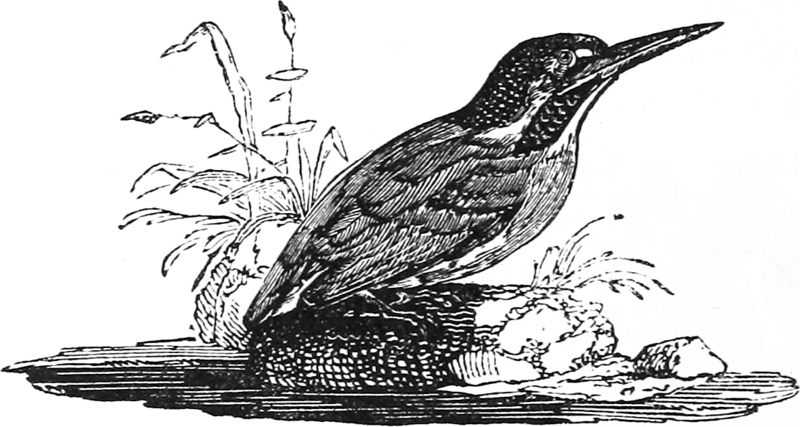
\includegraphics[scale=0.35]{images/Alycon.png}
        \end{figure}
        \vspace{0.5cm}
        \Huge
        \textbf{\textsc{Matematyka Dyskretna}}
        
        \vspace{0.5cm}
        \Large
        \textsc{Wybrane Dowody}
        
        \normalsize
        
        
        \line(1,0){330}
        
        \vspace{1cm}
        \textit{,,Myślę, że 7 punktów na 20 to nie jest zły wynik''}
        \vspace{1cm}

        \textit{\textsc{Popełnione przez}}\\
        \vspace{5mm}

        \textbf{\textsc{Dziurawy Ponton \\ Załatany Ponton \\ Puchaty Pompon \\ Zatopiony Ponton \\ Tonący Ponton \\ Notnop}}

        \vfill

        Kraków \\
        Anno Domini 2023
        
    \end{center}
    
\end{titlepage}


\tableofcontents
\section*{Licencja}
    \begin{figure}[h]
    	\begin{minipage}[c]{0.25\textwidth}
    		
\includegraphics[width=0.7\textwidth]{images/licencja.png}
    	\end{minipage}\hfill
    	\begin{minipage}[c]{0.75\textwidth}
    		\caption*{
    			Ten utwór jest dostępny na 
    			\href{https://creativecommons.org/licenses/by-sa/4.0/}{licencji Creative Commons Uznanie autorstwa
    			na tych samych warunkach 4.0 Międzynarodowe.}
    		}
    	\end{minipage}
    \end{figure}

% Actual content
\mainmatter

\chapter{Kombinatoryka}
 % Żeby nie było syfu to kolejne sekcje dodajemy do chapters/
% A potem includujemy za pomocą \input{chapters/...}

% Używamy \( \) i \[ \] zamiast dolarów -- tak jak się robi w LaTeXu


\documentclass[12pt, a4paper, polish, openany]{book}

% Please, let's familiarize ourselves with notatki.sty and tcs.sty so that we don't reinvent the wheel
\usepackage{notatki}

\fancyhead[L]{\textbf{\textit{MD}}}
\author{
}
\title{TCS and shitposting}


\begin{document}

% Front page and table of contents
\frontmatter

\input{titlepage}

\tableofcontents
\input{license}

% Actual content
\mainmatter

\chapter{Kombinatoryka}
\input{chapters/combinatorics/main}

\chapter{Zasada włączeń i wyłączeń}
\input{chapters/exclusion-inclusion/main}

\chapter{Posety}
\input{chapters/posets/main}

\chapter{Twierdzenie Ramseya}
\input{chapters/ramsey/main}

\chapter{Funkcje tworzące}
\input{chapters/generating_functions/main}

\chapter{Przepływy}
\input{chapters/flows/main}

\chapter{Skojarzenia}
\input{chapters/matchings/main}

\chapter{Kolorowanie grafów}
\input{chapters/graph-coloring/main}

\chapter{Grafy, ale nie kolorowanie}
\input{chapters/graph-misc/main}

\end{document}

\chapter{Zasada włączeń i wyłączeń}
 % Żeby nie było syfu to kolejne sekcje dodajemy do chapters/
% A potem includujemy za pomocą \input{chapters/...}

% Używamy \( \) i \[ \] zamiast dolarów -- tak jak się robi w LaTeXu


\documentclass[12pt, a4paper, polish, openany]{book}

% Please, let's familiarize ourselves with notatki.sty and tcs.sty so that we don't reinvent the wheel
\usepackage{notatki}

\fancyhead[L]{\textbf{\textit{MD}}}
\author{
}
\title{TCS and shitposting}


\begin{document}

% Front page and table of contents
\frontmatter

\input{titlepage}

\tableofcontents
\input{license}

% Actual content
\mainmatter

\chapter{Kombinatoryka}
\input{chapters/combinatorics/main}

\chapter{Zasada włączeń i wyłączeń}
\input{chapters/exclusion-inclusion/main}

\chapter{Posety}
\input{chapters/posets/main}

\chapter{Twierdzenie Ramseya}
\input{chapters/ramsey/main}

\chapter{Funkcje tworzące}
\input{chapters/generating_functions/main}

\chapter{Przepływy}
\input{chapters/flows/main}

\chapter{Skojarzenia}
\input{chapters/matchings/main}

\chapter{Kolorowanie grafów}
\input{chapters/graph-coloring/main}

\chapter{Grafy, ale nie kolorowanie}
\input{chapters/graph-misc/main}

\end{document}

\chapter{Posety}
 % Żeby nie było syfu to kolejne sekcje dodajemy do chapters/
% A potem includujemy za pomocą \input{chapters/...}

% Używamy \( \) i \[ \] zamiast dolarów -- tak jak się robi w LaTeXu


\documentclass[12pt, a4paper, polish, openany]{book}

% Please, let's familiarize ourselves with notatki.sty and tcs.sty so that we don't reinvent the wheel
\usepackage{notatki}

\fancyhead[L]{\textbf{\textit{MD}}}
\author{
}
\title{TCS and shitposting}


\begin{document}

% Front page and table of contents
\frontmatter

\input{titlepage}

\tableofcontents
\input{license}

% Actual content
\mainmatter

\chapter{Kombinatoryka}
\input{chapters/combinatorics/main}

\chapter{Zasada włączeń i wyłączeń}
\input{chapters/exclusion-inclusion/main}

\chapter{Posety}
\input{chapters/posets/main}

\chapter{Twierdzenie Ramseya}
\input{chapters/ramsey/main}

\chapter{Funkcje tworzące}
\input{chapters/generating_functions/main}

\chapter{Przepływy}
\input{chapters/flows/main}

\chapter{Skojarzenia}
\input{chapters/matchings/main}

\chapter{Kolorowanie grafów}
\input{chapters/graph-coloring/main}

\chapter{Grafy, ale nie kolorowanie}
\input{chapters/graph-misc/main}

\end{document}

\chapter{Twierdzenie Ramseya}
 % Żeby nie było syfu to kolejne sekcje dodajemy do chapters/
% A potem includujemy za pomocą \input{chapters/...}

% Używamy \( \) i \[ \] zamiast dolarów -- tak jak się robi w LaTeXu


\documentclass[12pt, a4paper, polish, openany]{book}

% Please, let's familiarize ourselves with notatki.sty and tcs.sty so that we don't reinvent the wheel
\usepackage{notatki}

\fancyhead[L]{\textbf{\textit{MD}}}
\author{
}
\title{TCS and shitposting}


\begin{document}

% Front page and table of contents
\frontmatter

\input{titlepage}

\tableofcontents
\input{license}

% Actual content
\mainmatter

\chapter{Kombinatoryka}
\input{chapters/combinatorics/main}

\chapter{Zasada włączeń i wyłączeń}
\input{chapters/exclusion-inclusion/main}

\chapter{Posety}
\input{chapters/posets/main}

\chapter{Twierdzenie Ramseya}
\input{chapters/ramsey/main}

\chapter{Funkcje tworzące}
\input{chapters/generating_functions/main}

\chapter{Przepływy}
\input{chapters/flows/main}

\chapter{Skojarzenia}
\input{chapters/matchings/main}

\chapter{Kolorowanie grafów}
\input{chapters/graph-coloring/main}

\chapter{Grafy, ale nie kolorowanie}
\input{chapters/graph-misc/main}

\end{document}

\chapter{Funkcje tworzące}
 % Żeby nie było syfu to kolejne sekcje dodajemy do chapters/
% A potem includujemy za pomocą \input{chapters/...}

% Używamy \( \) i \[ \] zamiast dolarów -- tak jak się robi w LaTeXu


\documentclass[12pt, a4paper, polish, openany]{book}

% Please, let's familiarize ourselves with notatki.sty and tcs.sty so that we don't reinvent the wheel
\usepackage{notatki}

\fancyhead[L]{\textbf{\textit{MD}}}
\author{
}
\title{TCS and shitposting}


\begin{document}

% Front page and table of contents
\frontmatter

\input{titlepage}

\tableofcontents
\input{license}

% Actual content
\mainmatter

\chapter{Kombinatoryka}
\input{chapters/combinatorics/main}

\chapter{Zasada włączeń i wyłączeń}
\input{chapters/exclusion-inclusion/main}

\chapter{Posety}
\input{chapters/posets/main}

\chapter{Twierdzenie Ramseya}
\input{chapters/ramsey/main}

\chapter{Funkcje tworzące}
\input{chapters/generating_functions/main}

\chapter{Przepływy}
\input{chapters/flows/main}

\chapter{Skojarzenia}
\input{chapters/matchings/main}

\chapter{Kolorowanie grafów}
\input{chapters/graph-coloring/main}

\chapter{Grafy, ale nie kolorowanie}
\input{chapters/graph-misc/main}

\end{document}

\chapter{Przepływy}
 % Żeby nie było syfu to kolejne sekcje dodajemy do chapters/
% A potem includujemy za pomocą \input{chapters/...}

% Używamy \( \) i \[ \] zamiast dolarów -- tak jak się robi w LaTeXu


\documentclass[12pt, a4paper, polish, openany]{book}

% Please, let's familiarize ourselves with notatki.sty and tcs.sty so that we don't reinvent the wheel
\usepackage{notatki}

\fancyhead[L]{\textbf{\textit{MD}}}
\author{
}
\title{TCS and shitposting}


\begin{document}

% Front page and table of contents
\frontmatter

\input{titlepage}

\tableofcontents
\input{license}

% Actual content
\mainmatter

\chapter{Kombinatoryka}
\input{chapters/combinatorics/main}

\chapter{Zasada włączeń i wyłączeń}
\input{chapters/exclusion-inclusion/main}

\chapter{Posety}
\input{chapters/posets/main}

\chapter{Twierdzenie Ramseya}
\input{chapters/ramsey/main}

\chapter{Funkcje tworzące}
\input{chapters/generating_functions/main}

\chapter{Przepływy}
\input{chapters/flows/main}

\chapter{Skojarzenia}
\input{chapters/matchings/main}

\chapter{Kolorowanie grafów}
\input{chapters/graph-coloring/main}

\chapter{Grafy, ale nie kolorowanie}
\input{chapters/graph-misc/main}

\end{document}

\chapter{Skojarzenia}
 % Żeby nie było syfu to kolejne sekcje dodajemy do chapters/
% A potem includujemy za pomocą \input{chapters/...}

% Używamy \( \) i \[ \] zamiast dolarów -- tak jak się robi w LaTeXu


\documentclass[12pt, a4paper, polish, openany]{book}

% Please, let's familiarize ourselves with notatki.sty and tcs.sty so that we don't reinvent the wheel
\usepackage{notatki}

\fancyhead[L]{\textbf{\textit{MD}}}
\author{
}
\title{TCS and shitposting}


\begin{document}

% Front page and table of contents
\frontmatter

\input{titlepage}

\tableofcontents
\input{license}

% Actual content
\mainmatter

\chapter{Kombinatoryka}
\input{chapters/combinatorics/main}

\chapter{Zasada włączeń i wyłączeń}
\input{chapters/exclusion-inclusion/main}

\chapter{Posety}
\input{chapters/posets/main}

\chapter{Twierdzenie Ramseya}
\input{chapters/ramsey/main}

\chapter{Funkcje tworzące}
\input{chapters/generating_functions/main}

\chapter{Przepływy}
\input{chapters/flows/main}

\chapter{Skojarzenia}
\input{chapters/matchings/main}

\chapter{Kolorowanie grafów}
\input{chapters/graph-coloring/main}

\chapter{Grafy, ale nie kolorowanie}
\input{chapters/graph-misc/main}

\end{document}

\chapter{Kolorowanie grafów}
 % Żeby nie było syfu to kolejne sekcje dodajemy do chapters/
% A potem includujemy za pomocą \input{chapters/...}

% Używamy \( \) i \[ \] zamiast dolarów -- tak jak się robi w LaTeXu


\documentclass[12pt, a4paper, polish, openany]{book}

% Please, let's familiarize ourselves with notatki.sty and tcs.sty so that we don't reinvent the wheel
\usepackage{notatki}

\fancyhead[L]{\textbf{\textit{MD}}}
\author{
}
\title{TCS and shitposting}


\begin{document}

% Front page and table of contents
\frontmatter

\input{titlepage}

\tableofcontents
\input{license}

% Actual content
\mainmatter

\chapter{Kombinatoryka}
\input{chapters/combinatorics/main}

\chapter{Zasada włączeń i wyłączeń}
\input{chapters/exclusion-inclusion/main}

\chapter{Posety}
\input{chapters/posets/main}

\chapter{Twierdzenie Ramseya}
\input{chapters/ramsey/main}

\chapter{Funkcje tworzące}
\input{chapters/generating_functions/main}

\chapter{Przepływy}
\input{chapters/flows/main}

\chapter{Skojarzenia}
\input{chapters/matchings/main}

\chapter{Kolorowanie grafów}
\input{chapters/graph-coloring/main}

\chapter{Grafy, ale nie kolorowanie}
\input{chapters/graph-misc/main}

\end{document}

\chapter{Grafy, ale nie kolorowanie}
 % Żeby nie było syfu to kolejne sekcje dodajemy do chapters/
% A potem includujemy za pomocą \input{chapters/...}

% Używamy \( \) i \[ \] zamiast dolarów -- tak jak się robi w LaTeXu


\documentclass[12pt, a4paper, polish, openany]{book}

% Please, let's familiarize ourselves with notatki.sty and tcs.sty so that we don't reinvent the wheel
\usepackage{notatki}

\fancyhead[L]{\textbf{\textit{MD}}}
\author{
}
\title{TCS and shitposting}


\begin{document}

% Front page and table of contents
\frontmatter

\input{titlepage}

\tableofcontents
\input{license}

% Actual content
\mainmatter

\chapter{Kombinatoryka}
\input{chapters/combinatorics/main}

\chapter{Zasada włączeń i wyłączeń}
\input{chapters/exclusion-inclusion/main}

\chapter{Posety}
\input{chapters/posets/main}

\chapter{Twierdzenie Ramseya}
\input{chapters/ramsey/main}

\chapter{Funkcje tworzące}
\input{chapters/generating_functions/main}

\chapter{Przepływy}
\input{chapters/flows/main}

\chapter{Skojarzenia}
\input{chapters/matchings/main}

\chapter{Kolorowanie grafów}
\input{chapters/graph-coloring/main}

\chapter{Grafy, ale nie kolorowanie}
\input{chapters/graph-misc/main}

\end{document}

\end{document}

\chapter{Twierdzenie Ramseya}
 % Żeby nie było syfu to kolejne sekcje dodajemy do chapters/
% A potem includujemy za pomocą \input{chapters/...}

% Używamy \( \) i \[ \] zamiast dolarów -- tak jak się robi w LaTeXu


\documentclass[12pt, a4paper, polish, openany]{book}

% Please, let's familiarize ourselves with notatki.sty and tcs.sty so that we don't reinvent the wheel
\usepackage{notatki}

\fancyhead[L]{\textbf{\textit{MD}}}
\author{
}
\title{TCS and shitposting}


\begin{document}

% Front page and table of contents
\frontmatter

\begin{titlepage} 

    \begin{center}
         \begin{figure}[h]
            \centering
            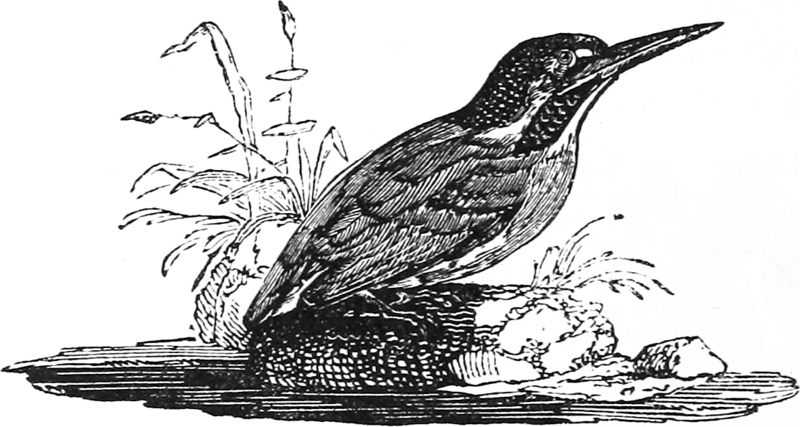
\includegraphics[scale=0.35]{images/Alycon.png}
        \end{figure}
        \vspace{0.5cm}
        \Huge
        \textbf{\textsc{Matematyka Dyskretna}}
        
        \vspace{0.5cm}
        \Large
        \textsc{Wybrane Dowody}
        
        \normalsize
        
        
        \line(1,0){330}
        
        \vspace{1cm}
        \textit{,,Myślę, że 7 punktów na 20 to nie jest zły wynik''}
        \vspace{1cm}

        \textit{\textsc{Popełnione przez}}\\
        \vspace{5mm}

        \textbf{\textsc{Dziurawy Ponton \\ Załatany Ponton \\ Puchaty Pompon \\ Zatopiony Ponton \\ Tonący Ponton \\ Notnop}}

        \vfill

        Kraków \\
        Anno Domini 2023
        
    \end{center}
    
\end{titlepage}


\tableofcontents
\section*{Licencja}
    \begin{figure}[h]
    	\begin{minipage}[c]{0.25\textwidth}
    		
\includegraphics[width=0.7\textwidth]{images/licencja.png}
    	\end{minipage}\hfill
    	\begin{minipage}[c]{0.75\textwidth}
    		\caption*{
    			Ten utwór jest dostępny na 
    			\href{https://creativecommons.org/licenses/by-sa/4.0/}{licencji Creative Commons Uznanie autorstwa
    			na tych samych warunkach 4.0 Międzynarodowe.}
    		}
    	\end{minipage}
    \end{figure}

% Actual content
\mainmatter

\chapter{Kombinatoryka}
 % Żeby nie było syfu to kolejne sekcje dodajemy do chapters/
% A potem includujemy za pomocą \input{chapters/...}

% Używamy \( \) i \[ \] zamiast dolarów -- tak jak się robi w LaTeXu


\documentclass[12pt, a4paper, polish, openany]{book}

% Please, let's familiarize ourselves with notatki.sty and tcs.sty so that we don't reinvent the wheel
\usepackage{notatki}

\fancyhead[L]{\textbf{\textit{MD}}}
\author{
}
\title{TCS and shitposting}


\begin{document}

% Front page and table of contents
\frontmatter

\input{titlepage}

\tableofcontents
\input{license}

% Actual content
\mainmatter

\chapter{Kombinatoryka}
\input{chapters/combinatorics/main}

\chapter{Zasada włączeń i wyłączeń}
\input{chapters/exclusion-inclusion/main}

\chapter{Posety}
\input{chapters/posets/main}

\chapter{Twierdzenie Ramseya}
\input{chapters/ramsey/main}

\chapter{Funkcje tworzące}
\input{chapters/generating_functions/main}

\chapter{Przepływy}
\input{chapters/flows/main}

\chapter{Skojarzenia}
\input{chapters/matchings/main}

\chapter{Kolorowanie grafów}
\input{chapters/graph-coloring/main}

\chapter{Grafy, ale nie kolorowanie}
\input{chapters/graph-misc/main}

\end{document}

\chapter{Zasada włączeń i wyłączeń}
 % Żeby nie było syfu to kolejne sekcje dodajemy do chapters/
% A potem includujemy za pomocą \input{chapters/...}

% Używamy \( \) i \[ \] zamiast dolarów -- tak jak się robi w LaTeXu


\documentclass[12pt, a4paper, polish, openany]{book}

% Please, let's familiarize ourselves with notatki.sty and tcs.sty so that we don't reinvent the wheel
\usepackage{notatki}

\fancyhead[L]{\textbf{\textit{MD}}}
\author{
}
\title{TCS and shitposting}


\begin{document}

% Front page and table of contents
\frontmatter

\input{titlepage}

\tableofcontents
\input{license}

% Actual content
\mainmatter

\chapter{Kombinatoryka}
\input{chapters/combinatorics/main}

\chapter{Zasada włączeń i wyłączeń}
\input{chapters/exclusion-inclusion/main}

\chapter{Posety}
\input{chapters/posets/main}

\chapter{Twierdzenie Ramseya}
\input{chapters/ramsey/main}

\chapter{Funkcje tworzące}
\input{chapters/generating_functions/main}

\chapter{Przepływy}
\input{chapters/flows/main}

\chapter{Skojarzenia}
\input{chapters/matchings/main}

\chapter{Kolorowanie grafów}
\input{chapters/graph-coloring/main}

\chapter{Grafy, ale nie kolorowanie}
\input{chapters/graph-misc/main}

\end{document}

\chapter{Posety}
 % Żeby nie było syfu to kolejne sekcje dodajemy do chapters/
% A potem includujemy za pomocą \input{chapters/...}

% Używamy \( \) i \[ \] zamiast dolarów -- tak jak się robi w LaTeXu


\documentclass[12pt, a4paper, polish, openany]{book}

% Please, let's familiarize ourselves with notatki.sty and tcs.sty so that we don't reinvent the wheel
\usepackage{notatki}

\fancyhead[L]{\textbf{\textit{MD}}}
\author{
}
\title{TCS and shitposting}


\begin{document}

% Front page and table of contents
\frontmatter

\input{titlepage}

\tableofcontents
\input{license}

% Actual content
\mainmatter

\chapter{Kombinatoryka}
\input{chapters/combinatorics/main}

\chapter{Zasada włączeń i wyłączeń}
\input{chapters/exclusion-inclusion/main}

\chapter{Posety}
\input{chapters/posets/main}

\chapter{Twierdzenie Ramseya}
\input{chapters/ramsey/main}

\chapter{Funkcje tworzące}
\input{chapters/generating_functions/main}

\chapter{Przepływy}
\input{chapters/flows/main}

\chapter{Skojarzenia}
\input{chapters/matchings/main}

\chapter{Kolorowanie grafów}
\input{chapters/graph-coloring/main}

\chapter{Grafy, ale nie kolorowanie}
\input{chapters/graph-misc/main}

\end{document}

\chapter{Twierdzenie Ramseya}
 % Żeby nie było syfu to kolejne sekcje dodajemy do chapters/
% A potem includujemy za pomocą \input{chapters/...}

% Używamy \( \) i \[ \] zamiast dolarów -- tak jak się robi w LaTeXu


\documentclass[12pt, a4paper, polish, openany]{book}

% Please, let's familiarize ourselves with notatki.sty and tcs.sty so that we don't reinvent the wheel
\usepackage{notatki}

\fancyhead[L]{\textbf{\textit{MD}}}
\author{
}
\title{TCS and shitposting}


\begin{document}

% Front page and table of contents
\frontmatter

\input{titlepage}

\tableofcontents
\input{license}

% Actual content
\mainmatter

\chapter{Kombinatoryka}
\input{chapters/combinatorics/main}

\chapter{Zasada włączeń i wyłączeń}
\input{chapters/exclusion-inclusion/main}

\chapter{Posety}
\input{chapters/posets/main}

\chapter{Twierdzenie Ramseya}
\input{chapters/ramsey/main}

\chapter{Funkcje tworzące}
\input{chapters/generating_functions/main}

\chapter{Przepływy}
\input{chapters/flows/main}

\chapter{Skojarzenia}
\input{chapters/matchings/main}

\chapter{Kolorowanie grafów}
\input{chapters/graph-coloring/main}

\chapter{Grafy, ale nie kolorowanie}
\input{chapters/graph-misc/main}

\end{document}

\chapter{Funkcje tworzące}
 % Żeby nie było syfu to kolejne sekcje dodajemy do chapters/
% A potem includujemy za pomocą \input{chapters/...}

% Używamy \( \) i \[ \] zamiast dolarów -- tak jak się robi w LaTeXu


\documentclass[12pt, a4paper, polish, openany]{book}

% Please, let's familiarize ourselves with notatki.sty and tcs.sty so that we don't reinvent the wheel
\usepackage{notatki}

\fancyhead[L]{\textbf{\textit{MD}}}
\author{
}
\title{TCS and shitposting}


\begin{document}

% Front page and table of contents
\frontmatter

\input{titlepage}

\tableofcontents
\input{license}

% Actual content
\mainmatter

\chapter{Kombinatoryka}
\input{chapters/combinatorics/main}

\chapter{Zasada włączeń i wyłączeń}
\input{chapters/exclusion-inclusion/main}

\chapter{Posety}
\input{chapters/posets/main}

\chapter{Twierdzenie Ramseya}
\input{chapters/ramsey/main}

\chapter{Funkcje tworzące}
\input{chapters/generating_functions/main}

\chapter{Przepływy}
\input{chapters/flows/main}

\chapter{Skojarzenia}
\input{chapters/matchings/main}

\chapter{Kolorowanie grafów}
\input{chapters/graph-coloring/main}

\chapter{Grafy, ale nie kolorowanie}
\input{chapters/graph-misc/main}

\end{document}

\chapter{Przepływy}
 % Żeby nie było syfu to kolejne sekcje dodajemy do chapters/
% A potem includujemy za pomocą \input{chapters/...}

% Używamy \( \) i \[ \] zamiast dolarów -- tak jak się robi w LaTeXu


\documentclass[12pt, a4paper, polish, openany]{book}

% Please, let's familiarize ourselves with notatki.sty and tcs.sty so that we don't reinvent the wheel
\usepackage{notatki}

\fancyhead[L]{\textbf{\textit{MD}}}
\author{
}
\title{TCS and shitposting}


\begin{document}

% Front page and table of contents
\frontmatter

\input{titlepage}

\tableofcontents
\input{license}

% Actual content
\mainmatter

\chapter{Kombinatoryka}
\input{chapters/combinatorics/main}

\chapter{Zasada włączeń i wyłączeń}
\input{chapters/exclusion-inclusion/main}

\chapter{Posety}
\input{chapters/posets/main}

\chapter{Twierdzenie Ramseya}
\input{chapters/ramsey/main}

\chapter{Funkcje tworzące}
\input{chapters/generating_functions/main}

\chapter{Przepływy}
\input{chapters/flows/main}

\chapter{Skojarzenia}
\input{chapters/matchings/main}

\chapter{Kolorowanie grafów}
\input{chapters/graph-coloring/main}

\chapter{Grafy, ale nie kolorowanie}
\input{chapters/graph-misc/main}

\end{document}

\chapter{Skojarzenia}
 % Żeby nie było syfu to kolejne sekcje dodajemy do chapters/
% A potem includujemy za pomocą \input{chapters/...}

% Używamy \( \) i \[ \] zamiast dolarów -- tak jak się robi w LaTeXu


\documentclass[12pt, a4paper, polish, openany]{book}

% Please, let's familiarize ourselves with notatki.sty and tcs.sty so that we don't reinvent the wheel
\usepackage{notatki}

\fancyhead[L]{\textbf{\textit{MD}}}
\author{
}
\title{TCS and shitposting}


\begin{document}

% Front page and table of contents
\frontmatter

\input{titlepage}

\tableofcontents
\input{license}

% Actual content
\mainmatter

\chapter{Kombinatoryka}
\input{chapters/combinatorics/main}

\chapter{Zasada włączeń i wyłączeń}
\input{chapters/exclusion-inclusion/main}

\chapter{Posety}
\input{chapters/posets/main}

\chapter{Twierdzenie Ramseya}
\input{chapters/ramsey/main}

\chapter{Funkcje tworzące}
\input{chapters/generating_functions/main}

\chapter{Przepływy}
\input{chapters/flows/main}

\chapter{Skojarzenia}
\input{chapters/matchings/main}

\chapter{Kolorowanie grafów}
\input{chapters/graph-coloring/main}

\chapter{Grafy, ale nie kolorowanie}
\input{chapters/graph-misc/main}

\end{document}

\chapter{Kolorowanie grafów}
 % Żeby nie było syfu to kolejne sekcje dodajemy do chapters/
% A potem includujemy za pomocą \input{chapters/...}

% Używamy \( \) i \[ \] zamiast dolarów -- tak jak się robi w LaTeXu


\documentclass[12pt, a4paper, polish, openany]{book}

% Please, let's familiarize ourselves with notatki.sty and tcs.sty so that we don't reinvent the wheel
\usepackage{notatki}

\fancyhead[L]{\textbf{\textit{MD}}}
\author{
}
\title{TCS and shitposting}


\begin{document}

% Front page and table of contents
\frontmatter

\input{titlepage}

\tableofcontents
\input{license}

% Actual content
\mainmatter

\chapter{Kombinatoryka}
\input{chapters/combinatorics/main}

\chapter{Zasada włączeń i wyłączeń}
\input{chapters/exclusion-inclusion/main}

\chapter{Posety}
\input{chapters/posets/main}

\chapter{Twierdzenie Ramseya}
\input{chapters/ramsey/main}

\chapter{Funkcje tworzące}
\input{chapters/generating_functions/main}

\chapter{Przepływy}
\input{chapters/flows/main}

\chapter{Skojarzenia}
\input{chapters/matchings/main}

\chapter{Kolorowanie grafów}
\input{chapters/graph-coloring/main}

\chapter{Grafy, ale nie kolorowanie}
\input{chapters/graph-misc/main}

\end{document}

\chapter{Grafy, ale nie kolorowanie}
 % Żeby nie było syfu to kolejne sekcje dodajemy do chapters/
% A potem includujemy za pomocą \input{chapters/...}

% Używamy \( \) i \[ \] zamiast dolarów -- tak jak się robi w LaTeXu


\documentclass[12pt, a4paper, polish, openany]{book}

% Please, let's familiarize ourselves with notatki.sty and tcs.sty so that we don't reinvent the wheel
\usepackage{notatki}

\fancyhead[L]{\textbf{\textit{MD}}}
\author{
}
\title{TCS and shitposting}


\begin{document}

% Front page and table of contents
\frontmatter

\input{titlepage}

\tableofcontents
\input{license}

% Actual content
\mainmatter

\chapter{Kombinatoryka}
\input{chapters/combinatorics/main}

\chapter{Zasada włączeń i wyłączeń}
\input{chapters/exclusion-inclusion/main}

\chapter{Posety}
\input{chapters/posets/main}

\chapter{Twierdzenie Ramseya}
\input{chapters/ramsey/main}

\chapter{Funkcje tworzące}
\input{chapters/generating_functions/main}

\chapter{Przepływy}
\input{chapters/flows/main}

\chapter{Skojarzenia}
\input{chapters/matchings/main}

\chapter{Kolorowanie grafów}
\input{chapters/graph-coloring/main}

\chapter{Grafy, ale nie kolorowanie}
\input{chapters/graph-misc/main}

\end{document}

\end{document}

\chapter{Funkcje tworzące}
 % Żeby nie było syfu to kolejne sekcje dodajemy do chapters/
% A potem includujemy za pomocą \input{chapters/...}

% Używamy \( \) i \[ \] zamiast dolarów -- tak jak się robi w LaTeXu


\documentclass[12pt, a4paper, polish, openany]{book}

% Please, let's familiarize ourselves with notatki.sty and tcs.sty so that we don't reinvent the wheel
\usepackage{notatki}

\fancyhead[L]{\textbf{\textit{MD}}}
\author{
}
\title{TCS and shitposting}


\begin{document}

% Front page and table of contents
\frontmatter

\begin{titlepage} 

    \begin{center}
         \begin{figure}[h]
            \centering
            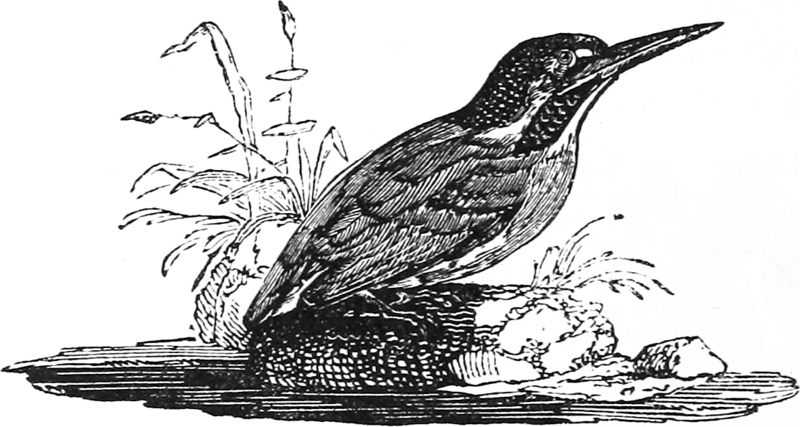
\includegraphics[scale=0.35]{images/Alycon.png}
        \end{figure}
        \vspace{0.5cm}
        \Huge
        \textbf{\textsc{Matematyka Dyskretna}}
        
        \vspace{0.5cm}
        \Large
        \textsc{Wybrane Dowody}
        
        \normalsize
        
        
        \line(1,0){330}
        
        \vspace{1cm}
        \textit{,,Myślę, że 7 punktów na 20 to nie jest zły wynik''}
        \vspace{1cm}

        \textit{\textsc{Popełnione przez}}\\
        \vspace{5mm}

        \textbf{\textsc{Dziurawy Ponton \\ Załatany Ponton \\ Puchaty Pompon \\ Zatopiony Ponton \\ Tonący Ponton \\ Notnop}}

        \vfill

        Kraków \\
        Anno Domini 2023
        
    \end{center}
    
\end{titlepage}


\tableofcontents
\section*{Licencja}
    \begin{figure}[h]
    	\begin{minipage}[c]{0.25\textwidth}
    		
\includegraphics[width=0.7\textwidth]{images/licencja.png}
    	\end{minipage}\hfill
    	\begin{minipage}[c]{0.75\textwidth}
    		\caption*{
    			Ten utwór jest dostępny na 
    			\href{https://creativecommons.org/licenses/by-sa/4.0/}{licencji Creative Commons Uznanie autorstwa
    			na tych samych warunkach 4.0 Międzynarodowe.}
    		}
    	\end{minipage}
    \end{figure}

% Actual content
\mainmatter

\chapter{Kombinatoryka}
 % Żeby nie było syfu to kolejne sekcje dodajemy do chapters/
% A potem includujemy za pomocą \input{chapters/...}

% Używamy \( \) i \[ \] zamiast dolarów -- tak jak się robi w LaTeXu


\documentclass[12pt, a4paper, polish, openany]{book}

% Please, let's familiarize ourselves with notatki.sty and tcs.sty so that we don't reinvent the wheel
\usepackage{notatki}

\fancyhead[L]{\textbf{\textit{MD}}}
\author{
}
\title{TCS and shitposting}


\begin{document}

% Front page and table of contents
\frontmatter

\input{titlepage}

\tableofcontents
\input{license}

% Actual content
\mainmatter

\chapter{Kombinatoryka}
\input{chapters/combinatorics/main}

\chapter{Zasada włączeń i wyłączeń}
\input{chapters/exclusion-inclusion/main}

\chapter{Posety}
\input{chapters/posets/main}

\chapter{Twierdzenie Ramseya}
\input{chapters/ramsey/main}

\chapter{Funkcje tworzące}
\input{chapters/generating_functions/main}

\chapter{Przepływy}
\input{chapters/flows/main}

\chapter{Skojarzenia}
\input{chapters/matchings/main}

\chapter{Kolorowanie grafów}
\input{chapters/graph-coloring/main}

\chapter{Grafy, ale nie kolorowanie}
\input{chapters/graph-misc/main}

\end{document}

\chapter{Zasada włączeń i wyłączeń}
 % Żeby nie było syfu to kolejne sekcje dodajemy do chapters/
% A potem includujemy za pomocą \input{chapters/...}

% Używamy \( \) i \[ \] zamiast dolarów -- tak jak się robi w LaTeXu


\documentclass[12pt, a4paper, polish, openany]{book}

% Please, let's familiarize ourselves with notatki.sty and tcs.sty so that we don't reinvent the wheel
\usepackage{notatki}

\fancyhead[L]{\textbf{\textit{MD}}}
\author{
}
\title{TCS and shitposting}


\begin{document}

% Front page and table of contents
\frontmatter

\input{titlepage}

\tableofcontents
\input{license}

% Actual content
\mainmatter

\chapter{Kombinatoryka}
\input{chapters/combinatorics/main}

\chapter{Zasada włączeń i wyłączeń}
\input{chapters/exclusion-inclusion/main}

\chapter{Posety}
\input{chapters/posets/main}

\chapter{Twierdzenie Ramseya}
\input{chapters/ramsey/main}

\chapter{Funkcje tworzące}
\input{chapters/generating_functions/main}

\chapter{Przepływy}
\input{chapters/flows/main}

\chapter{Skojarzenia}
\input{chapters/matchings/main}

\chapter{Kolorowanie grafów}
\input{chapters/graph-coloring/main}

\chapter{Grafy, ale nie kolorowanie}
\input{chapters/graph-misc/main}

\end{document}

\chapter{Posety}
 % Żeby nie było syfu to kolejne sekcje dodajemy do chapters/
% A potem includujemy za pomocą \input{chapters/...}

% Używamy \( \) i \[ \] zamiast dolarów -- tak jak się robi w LaTeXu


\documentclass[12pt, a4paper, polish, openany]{book}

% Please, let's familiarize ourselves with notatki.sty and tcs.sty so that we don't reinvent the wheel
\usepackage{notatki}

\fancyhead[L]{\textbf{\textit{MD}}}
\author{
}
\title{TCS and shitposting}


\begin{document}

% Front page and table of contents
\frontmatter

\input{titlepage}

\tableofcontents
\input{license}

% Actual content
\mainmatter

\chapter{Kombinatoryka}
\input{chapters/combinatorics/main}

\chapter{Zasada włączeń i wyłączeń}
\input{chapters/exclusion-inclusion/main}

\chapter{Posety}
\input{chapters/posets/main}

\chapter{Twierdzenie Ramseya}
\input{chapters/ramsey/main}

\chapter{Funkcje tworzące}
\input{chapters/generating_functions/main}

\chapter{Przepływy}
\input{chapters/flows/main}

\chapter{Skojarzenia}
\input{chapters/matchings/main}

\chapter{Kolorowanie grafów}
\input{chapters/graph-coloring/main}

\chapter{Grafy, ale nie kolorowanie}
\input{chapters/graph-misc/main}

\end{document}

\chapter{Twierdzenie Ramseya}
 % Żeby nie było syfu to kolejne sekcje dodajemy do chapters/
% A potem includujemy za pomocą \input{chapters/...}

% Używamy \( \) i \[ \] zamiast dolarów -- tak jak się robi w LaTeXu


\documentclass[12pt, a4paper, polish, openany]{book}

% Please, let's familiarize ourselves with notatki.sty and tcs.sty so that we don't reinvent the wheel
\usepackage{notatki}

\fancyhead[L]{\textbf{\textit{MD}}}
\author{
}
\title{TCS and shitposting}


\begin{document}

% Front page and table of contents
\frontmatter

\input{titlepage}

\tableofcontents
\input{license}

% Actual content
\mainmatter

\chapter{Kombinatoryka}
\input{chapters/combinatorics/main}

\chapter{Zasada włączeń i wyłączeń}
\input{chapters/exclusion-inclusion/main}

\chapter{Posety}
\input{chapters/posets/main}

\chapter{Twierdzenie Ramseya}
\input{chapters/ramsey/main}

\chapter{Funkcje tworzące}
\input{chapters/generating_functions/main}

\chapter{Przepływy}
\input{chapters/flows/main}

\chapter{Skojarzenia}
\input{chapters/matchings/main}

\chapter{Kolorowanie grafów}
\input{chapters/graph-coloring/main}

\chapter{Grafy, ale nie kolorowanie}
\input{chapters/graph-misc/main}

\end{document}

\chapter{Funkcje tworzące}
 % Żeby nie było syfu to kolejne sekcje dodajemy do chapters/
% A potem includujemy za pomocą \input{chapters/...}

% Używamy \( \) i \[ \] zamiast dolarów -- tak jak się robi w LaTeXu


\documentclass[12pt, a4paper, polish, openany]{book}

% Please, let's familiarize ourselves with notatki.sty and tcs.sty so that we don't reinvent the wheel
\usepackage{notatki}

\fancyhead[L]{\textbf{\textit{MD}}}
\author{
}
\title{TCS and shitposting}


\begin{document}

% Front page and table of contents
\frontmatter

\input{titlepage}

\tableofcontents
\input{license}

% Actual content
\mainmatter

\chapter{Kombinatoryka}
\input{chapters/combinatorics/main}

\chapter{Zasada włączeń i wyłączeń}
\input{chapters/exclusion-inclusion/main}

\chapter{Posety}
\input{chapters/posets/main}

\chapter{Twierdzenie Ramseya}
\input{chapters/ramsey/main}

\chapter{Funkcje tworzące}
\input{chapters/generating_functions/main}

\chapter{Przepływy}
\input{chapters/flows/main}

\chapter{Skojarzenia}
\input{chapters/matchings/main}

\chapter{Kolorowanie grafów}
\input{chapters/graph-coloring/main}

\chapter{Grafy, ale nie kolorowanie}
\input{chapters/graph-misc/main}

\end{document}

\chapter{Przepływy}
 % Żeby nie było syfu to kolejne sekcje dodajemy do chapters/
% A potem includujemy za pomocą \input{chapters/...}

% Używamy \( \) i \[ \] zamiast dolarów -- tak jak się robi w LaTeXu


\documentclass[12pt, a4paper, polish, openany]{book}

% Please, let's familiarize ourselves with notatki.sty and tcs.sty so that we don't reinvent the wheel
\usepackage{notatki}

\fancyhead[L]{\textbf{\textit{MD}}}
\author{
}
\title{TCS and shitposting}


\begin{document}

% Front page and table of contents
\frontmatter

\input{titlepage}

\tableofcontents
\input{license}

% Actual content
\mainmatter

\chapter{Kombinatoryka}
\input{chapters/combinatorics/main}

\chapter{Zasada włączeń i wyłączeń}
\input{chapters/exclusion-inclusion/main}

\chapter{Posety}
\input{chapters/posets/main}

\chapter{Twierdzenie Ramseya}
\input{chapters/ramsey/main}

\chapter{Funkcje tworzące}
\input{chapters/generating_functions/main}

\chapter{Przepływy}
\input{chapters/flows/main}

\chapter{Skojarzenia}
\input{chapters/matchings/main}

\chapter{Kolorowanie grafów}
\input{chapters/graph-coloring/main}

\chapter{Grafy, ale nie kolorowanie}
\input{chapters/graph-misc/main}

\end{document}

\chapter{Skojarzenia}
 % Żeby nie było syfu to kolejne sekcje dodajemy do chapters/
% A potem includujemy za pomocą \input{chapters/...}

% Używamy \( \) i \[ \] zamiast dolarów -- tak jak się robi w LaTeXu


\documentclass[12pt, a4paper, polish, openany]{book}

% Please, let's familiarize ourselves with notatki.sty and tcs.sty so that we don't reinvent the wheel
\usepackage{notatki}

\fancyhead[L]{\textbf{\textit{MD}}}
\author{
}
\title{TCS and shitposting}


\begin{document}

% Front page and table of contents
\frontmatter

\input{titlepage}

\tableofcontents
\input{license}

% Actual content
\mainmatter

\chapter{Kombinatoryka}
\input{chapters/combinatorics/main}

\chapter{Zasada włączeń i wyłączeń}
\input{chapters/exclusion-inclusion/main}

\chapter{Posety}
\input{chapters/posets/main}

\chapter{Twierdzenie Ramseya}
\input{chapters/ramsey/main}

\chapter{Funkcje tworzące}
\input{chapters/generating_functions/main}

\chapter{Przepływy}
\input{chapters/flows/main}

\chapter{Skojarzenia}
\input{chapters/matchings/main}

\chapter{Kolorowanie grafów}
\input{chapters/graph-coloring/main}

\chapter{Grafy, ale nie kolorowanie}
\input{chapters/graph-misc/main}

\end{document}

\chapter{Kolorowanie grafów}
 % Żeby nie było syfu to kolejne sekcje dodajemy do chapters/
% A potem includujemy za pomocą \input{chapters/...}

% Używamy \( \) i \[ \] zamiast dolarów -- tak jak się robi w LaTeXu


\documentclass[12pt, a4paper, polish, openany]{book}

% Please, let's familiarize ourselves with notatki.sty and tcs.sty so that we don't reinvent the wheel
\usepackage{notatki}

\fancyhead[L]{\textbf{\textit{MD}}}
\author{
}
\title{TCS and shitposting}


\begin{document}

% Front page and table of contents
\frontmatter

\input{titlepage}

\tableofcontents
\input{license}

% Actual content
\mainmatter

\chapter{Kombinatoryka}
\input{chapters/combinatorics/main}

\chapter{Zasada włączeń i wyłączeń}
\input{chapters/exclusion-inclusion/main}

\chapter{Posety}
\input{chapters/posets/main}

\chapter{Twierdzenie Ramseya}
\input{chapters/ramsey/main}

\chapter{Funkcje tworzące}
\input{chapters/generating_functions/main}

\chapter{Przepływy}
\input{chapters/flows/main}

\chapter{Skojarzenia}
\input{chapters/matchings/main}

\chapter{Kolorowanie grafów}
\input{chapters/graph-coloring/main}

\chapter{Grafy, ale nie kolorowanie}
\input{chapters/graph-misc/main}

\end{document}

\chapter{Grafy, ale nie kolorowanie}
 % Żeby nie było syfu to kolejne sekcje dodajemy do chapters/
% A potem includujemy za pomocą \input{chapters/...}

% Używamy \( \) i \[ \] zamiast dolarów -- tak jak się robi w LaTeXu


\documentclass[12pt, a4paper, polish, openany]{book}

% Please, let's familiarize ourselves with notatki.sty and tcs.sty so that we don't reinvent the wheel
\usepackage{notatki}

\fancyhead[L]{\textbf{\textit{MD}}}
\author{
}
\title{TCS and shitposting}


\begin{document}

% Front page and table of contents
\frontmatter

\input{titlepage}

\tableofcontents
\input{license}

% Actual content
\mainmatter

\chapter{Kombinatoryka}
\input{chapters/combinatorics/main}

\chapter{Zasada włączeń i wyłączeń}
\input{chapters/exclusion-inclusion/main}

\chapter{Posety}
\input{chapters/posets/main}

\chapter{Twierdzenie Ramseya}
\input{chapters/ramsey/main}

\chapter{Funkcje tworzące}
\input{chapters/generating_functions/main}

\chapter{Przepływy}
\input{chapters/flows/main}

\chapter{Skojarzenia}
\input{chapters/matchings/main}

\chapter{Kolorowanie grafów}
\input{chapters/graph-coloring/main}

\chapter{Grafy, ale nie kolorowanie}
\input{chapters/graph-misc/main}

\end{document}

\end{document}

\chapter{Przepływy}
 % Żeby nie było syfu to kolejne sekcje dodajemy do chapters/
% A potem includujemy za pomocą \input{chapters/...}

% Używamy \( \) i \[ \] zamiast dolarów -- tak jak się robi w LaTeXu


\documentclass[12pt, a4paper, polish, openany]{book}

% Please, let's familiarize ourselves with notatki.sty and tcs.sty so that we don't reinvent the wheel
\usepackage{notatki}

\fancyhead[L]{\textbf{\textit{MD}}}
\author{
}
\title{TCS and shitposting}


\begin{document}

% Front page and table of contents
\frontmatter

\begin{titlepage} 

    \begin{center}
         \begin{figure}[h]
            \centering
            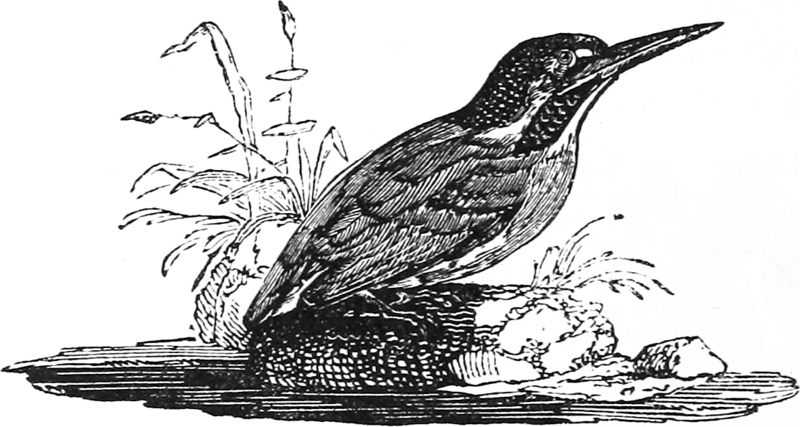
\includegraphics[scale=0.35]{images/Alycon.png}
        \end{figure}
        \vspace{0.5cm}
        \Huge
        \textbf{\textsc{Matematyka Dyskretna}}
        
        \vspace{0.5cm}
        \Large
        \textsc{Wybrane Dowody}
        
        \normalsize
        
        
        \line(1,0){330}
        
        \vspace{1cm}
        \textit{,,Myślę, że 7 punktów na 20 to nie jest zły wynik''}
        \vspace{1cm}

        \textit{\textsc{Popełnione przez}}\\
        \vspace{5mm}

        \textbf{\textsc{Dziurawy Ponton \\ Załatany Ponton \\ Puchaty Pompon \\ Zatopiony Ponton \\ Tonący Ponton \\ Notnop}}

        \vfill

        Kraków \\
        Anno Domini 2023
        
    \end{center}
    
\end{titlepage}


\tableofcontents
\section*{Licencja}
    \begin{figure}[h]
    	\begin{minipage}[c]{0.25\textwidth}
    		
\includegraphics[width=0.7\textwidth]{images/licencja.png}
    	\end{minipage}\hfill
    	\begin{minipage}[c]{0.75\textwidth}
    		\caption*{
    			Ten utwór jest dostępny na 
    			\href{https://creativecommons.org/licenses/by-sa/4.0/}{licencji Creative Commons Uznanie autorstwa
    			na tych samych warunkach 4.0 Międzynarodowe.}
    		}
    	\end{minipage}
    \end{figure}

% Actual content
\mainmatter

\chapter{Kombinatoryka}
 % Żeby nie było syfu to kolejne sekcje dodajemy do chapters/
% A potem includujemy za pomocą \input{chapters/...}

% Używamy \( \) i \[ \] zamiast dolarów -- tak jak się robi w LaTeXu


\documentclass[12pt, a4paper, polish, openany]{book}

% Please, let's familiarize ourselves with notatki.sty and tcs.sty so that we don't reinvent the wheel
\usepackage{notatki}

\fancyhead[L]{\textbf{\textit{MD}}}
\author{
}
\title{TCS and shitposting}


\begin{document}

% Front page and table of contents
\frontmatter

\input{titlepage}

\tableofcontents
\input{license}

% Actual content
\mainmatter

\chapter{Kombinatoryka}
\input{chapters/combinatorics/main}

\chapter{Zasada włączeń i wyłączeń}
\input{chapters/exclusion-inclusion/main}

\chapter{Posety}
\input{chapters/posets/main}

\chapter{Twierdzenie Ramseya}
\input{chapters/ramsey/main}

\chapter{Funkcje tworzące}
\input{chapters/generating_functions/main}

\chapter{Przepływy}
\input{chapters/flows/main}

\chapter{Skojarzenia}
\input{chapters/matchings/main}

\chapter{Kolorowanie grafów}
\input{chapters/graph-coloring/main}

\chapter{Grafy, ale nie kolorowanie}
\input{chapters/graph-misc/main}

\end{document}

\chapter{Zasada włączeń i wyłączeń}
 % Żeby nie było syfu to kolejne sekcje dodajemy do chapters/
% A potem includujemy za pomocą \input{chapters/...}

% Używamy \( \) i \[ \] zamiast dolarów -- tak jak się robi w LaTeXu


\documentclass[12pt, a4paper, polish, openany]{book}

% Please, let's familiarize ourselves with notatki.sty and tcs.sty so that we don't reinvent the wheel
\usepackage{notatki}

\fancyhead[L]{\textbf{\textit{MD}}}
\author{
}
\title{TCS and shitposting}


\begin{document}

% Front page and table of contents
\frontmatter

\input{titlepage}

\tableofcontents
\input{license}

% Actual content
\mainmatter

\chapter{Kombinatoryka}
\input{chapters/combinatorics/main}

\chapter{Zasada włączeń i wyłączeń}
\input{chapters/exclusion-inclusion/main}

\chapter{Posety}
\input{chapters/posets/main}

\chapter{Twierdzenie Ramseya}
\input{chapters/ramsey/main}

\chapter{Funkcje tworzące}
\input{chapters/generating_functions/main}

\chapter{Przepływy}
\input{chapters/flows/main}

\chapter{Skojarzenia}
\input{chapters/matchings/main}

\chapter{Kolorowanie grafów}
\input{chapters/graph-coloring/main}

\chapter{Grafy, ale nie kolorowanie}
\input{chapters/graph-misc/main}

\end{document}

\chapter{Posety}
 % Żeby nie było syfu to kolejne sekcje dodajemy do chapters/
% A potem includujemy za pomocą \input{chapters/...}

% Używamy \( \) i \[ \] zamiast dolarów -- tak jak się robi w LaTeXu


\documentclass[12pt, a4paper, polish, openany]{book}

% Please, let's familiarize ourselves with notatki.sty and tcs.sty so that we don't reinvent the wheel
\usepackage{notatki}

\fancyhead[L]{\textbf{\textit{MD}}}
\author{
}
\title{TCS and shitposting}


\begin{document}

% Front page and table of contents
\frontmatter

\input{titlepage}

\tableofcontents
\input{license}

% Actual content
\mainmatter

\chapter{Kombinatoryka}
\input{chapters/combinatorics/main}

\chapter{Zasada włączeń i wyłączeń}
\input{chapters/exclusion-inclusion/main}

\chapter{Posety}
\input{chapters/posets/main}

\chapter{Twierdzenie Ramseya}
\input{chapters/ramsey/main}

\chapter{Funkcje tworzące}
\input{chapters/generating_functions/main}

\chapter{Przepływy}
\input{chapters/flows/main}

\chapter{Skojarzenia}
\input{chapters/matchings/main}

\chapter{Kolorowanie grafów}
\input{chapters/graph-coloring/main}

\chapter{Grafy, ale nie kolorowanie}
\input{chapters/graph-misc/main}

\end{document}

\chapter{Twierdzenie Ramseya}
 % Żeby nie było syfu to kolejne sekcje dodajemy do chapters/
% A potem includujemy za pomocą \input{chapters/...}

% Używamy \( \) i \[ \] zamiast dolarów -- tak jak się robi w LaTeXu


\documentclass[12pt, a4paper, polish, openany]{book}

% Please, let's familiarize ourselves with notatki.sty and tcs.sty so that we don't reinvent the wheel
\usepackage{notatki}

\fancyhead[L]{\textbf{\textit{MD}}}
\author{
}
\title{TCS and shitposting}


\begin{document}

% Front page and table of contents
\frontmatter

\input{titlepage}

\tableofcontents
\input{license}

% Actual content
\mainmatter

\chapter{Kombinatoryka}
\input{chapters/combinatorics/main}

\chapter{Zasada włączeń i wyłączeń}
\input{chapters/exclusion-inclusion/main}

\chapter{Posety}
\input{chapters/posets/main}

\chapter{Twierdzenie Ramseya}
\input{chapters/ramsey/main}

\chapter{Funkcje tworzące}
\input{chapters/generating_functions/main}

\chapter{Przepływy}
\input{chapters/flows/main}

\chapter{Skojarzenia}
\input{chapters/matchings/main}

\chapter{Kolorowanie grafów}
\input{chapters/graph-coloring/main}

\chapter{Grafy, ale nie kolorowanie}
\input{chapters/graph-misc/main}

\end{document}

\chapter{Funkcje tworzące}
 % Żeby nie było syfu to kolejne sekcje dodajemy do chapters/
% A potem includujemy za pomocą \input{chapters/...}

% Używamy \( \) i \[ \] zamiast dolarów -- tak jak się robi w LaTeXu


\documentclass[12pt, a4paper, polish, openany]{book}

% Please, let's familiarize ourselves with notatki.sty and tcs.sty so that we don't reinvent the wheel
\usepackage{notatki}

\fancyhead[L]{\textbf{\textit{MD}}}
\author{
}
\title{TCS and shitposting}


\begin{document}

% Front page and table of contents
\frontmatter

\input{titlepage}

\tableofcontents
\input{license}

% Actual content
\mainmatter

\chapter{Kombinatoryka}
\input{chapters/combinatorics/main}

\chapter{Zasada włączeń i wyłączeń}
\input{chapters/exclusion-inclusion/main}

\chapter{Posety}
\input{chapters/posets/main}

\chapter{Twierdzenie Ramseya}
\input{chapters/ramsey/main}

\chapter{Funkcje tworzące}
\input{chapters/generating_functions/main}

\chapter{Przepływy}
\input{chapters/flows/main}

\chapter{Skojarzenia}
\input{chapters/matchings/main}

\chapter{Kolorowanie grafów}
\input{chapters/graph-coloring/main}

\chapter{Grafy, ale nie kolorowanie}
\input{chapters/graph-misc/main}

\end{document}

\chapter{Przepływy}
 % Żeby nie było syfu to kolejne sekcje dodajemy do chapters/
% A potem includujemy za pomocą \input{chapters/...}

% Używamy \( \) i \[ \] zamiast dolarów -- tak jak się robi w LaTeXu


\documentclass[12pt, a4paper, polish, openany]{book}

% Please, let's familiarize ourselves with notatki.sty and tcs.sty so that we don't reinvent the wheel
\usepackage{notatki}

\fancyhead[L]{\textbf{\textit{MD}}}
\author{
}
\title{TCS and shitposting}


\begin{document}

% Front page and table of contents
\frontmatter

\input{titlepage}

\tableofcontents
\input{license}

% Actual content
\mainmatter

\chapter{Kombinatoryka}
\input{chapters/combinatorics/main}

\chapter{Zasada włączeń i wyłączeń}
\input{chapters/exclusion-inclusion/main}

\chapter{Posety}
\input{chapters/posets/main}

\chapter{Twierdzenie Ramseya}
\input{chapters/ramsey/main}

\chapter{Funkcje tworzące}
\input{chapters/generating_functions/main}

\chapter{Przepływy}
\input{chapters/flows/main}

\chapter{Skojarzenia}
\input{chapters/matchings/main}

\chapter{Kolorowanie grafów}
\input{chapters/graph-coloring/main}

\chapter{Grafy, ale nie kolorowanie}
\input{chapters/graph-misc/main}

\end{document}

\chapter{Skojarzenia}
 % Żeby nie było syfu to kolejne sekcje dodajemy do chapters/
% A potem includujemy za pomocą \input{chapters/...}

% Używamy \( \) i \[ \] zamiast dolarów -- tak jak się robi w LaTeXu


\documentclass[12pt, a4paper, polish, openany]{book}

% Please, let's familiarize ourselves with notatki.sty and tcs.sty so that we don't reinvent the wheel
\usepackage{notatki}

\fancyhead[L]{\textbf{\textit{MD}}}
\author{
}
\title{TCS and shitposting}


\begin{document}

% Front page and table of contents
\frontmatter

\input{titlepage}

\tableofcontents
\input{license}

% Actual content
\mainmatter

\chapter{Kombinatoryka}
\input{chapters/combinatorics/main}

\chapter{Zasada włączeń i wyłączeń}
\input{chapters/exclusion-inclusion/main}

\chapter{Posety}
\input{chapters/posets/main}

\chapter{Twierdzenie Ramseya}
\input{chapters/ramsey/main}

\chapter{Funkcje tworzące}
\input{chapters/generating_functions/main}

\chapter{Przepływy}
\input{chapters/flows/main}

\chapter{Skojarzenia}
\input{chapters/matchings/main}

\chapter{Kolorowanie grafów}
\input{chapters/graph-coloring/main}

\chapter{Grafy, ale nie kolorowanie}
\input{chapters/graph-misc/main}

\end{document}

\chapter{Kolorowanie grafów}
 % Żeby nie było syfu to kolejne sekcje dodajemy do chapters/
% A potem includujemy za pomocą \input{chapters/...}

% Używamy \( \) i \[ \] zamiast dolarów -- tak jak się robi w LaTeXu


\documentclass[12pt, a4paper, polish, openany]{book}

% Please, let's familiarize ourselves with notatki.sty and tcs.sty so that we don't reinvent the wheel
\usepackage{notatki}

\fancyhead[L]{\textbf{\textit{MD}}}
\author{
}
\title{TCS and shitposting}


\begin{document}

% Front page and table of contents
\frontmatter

\input{titlepage}

\tableofcontents
\input{license}

% Actual content
\mainmatter

\chapter{Kombinatoryka}
\input{chapters/combinatorics/main}

\chapter{Zasada włączeń i wyłączeń}
\input{chapters/exclusion-inclusion/main}

\chapter{Posety}
\input{chapters/posets/main}

\chapter{Twierdzenie Ramseya}
\input{chapters/ramsey/main}

\chapter{Funkcje tworzące}
\input{chapters/generating_functions/main}

\chapter{Przepływy}
\input{chapters/flows/main}

\chapter{Skojarzenia}
\input{chapters/matchings/main}

\chapter{Kolorowanie grafów}
\input{chapters/graph-coloring/main}

\chapter{Grafy, ale nie kolorowanie}
\input{chapters/graph-misc/main}

\end{document}

\chapter{Grafy, ale nie kolorowanie}
 % Żeby nie było syfu to kolejne sekcje dodajemy do chapters/
% A potem includujemy za pomocą \input{chapters/...}

% Używamy \( \) i \[ \] zamiast dolarów -- tak jak się robi w LaTeXu


\documentclass[12pt, a4paper, polish, openany]{book}

% Please, let's familiarize ourselves with notatki.sty and tcs.sty so that we don't reinvent the wheel
\usepackage{notatki}

\fancyhead[L]{\textbf{\textit{MD}}}
\author{
}
\title{TCS and shitposting}


\begin{document}

% Front page and table of contents
\frontmatter

\input{titlepage}

\tableofcontents
\input{license}

% Actual content
\mainmatter

\chapter{Kombinatoryka}
\input{chapters/combinatorics/main}

\chapter{Zasada włączeń i wyłączeń}
\input{chapters/exclusion-inclusion/main}

\chapter{Posety}
\input{chapters/posets/main}

\chapter{Twierdzenie Ramseya}
\input{chapters/ramsey/main}

\chapter{Funkcje tworzące}
\input{chapters/generating_functions/main}

\chapter{Przepływy}
\input{chapters/flows/main}

\chapter{Skojarzenia}
\input{chapters/matchings/main}

\chapter{Kolorowanie grafów}
\input{chapters/graph-coloring/main}

\chapter{Grafy, ale nie kolorowanie}
\input{chapters/graph-misc/main}

\end{document}

\end{document}

\chapter{Skojarzenia}
 % Żeby nie było syfu to kolejne sekcje dodajemy do chapters/
% A potem includujemy za pomocą \input{chapters/...}

% Używamy \( \) i \[ \] zamiast dolarów -- tak jak się robi w LaTeXu


\documentclass[12pt, a4paper, polish, openany]{book}

% Please, let's familiarize ourselves with notatki.sty and tcs.sty so that we don't reinvent the wheel
\usepackage{notatki}

\fancyhead[L]{\textbf{\textit{MD}}}
\author{
}
\title{TCS and shitposting}


\begin{document}

% Front page and table of contents
\frontmatter

\begin{titlepage} 

    \begin{center}
         \begin{figure}[h]
            \centering
            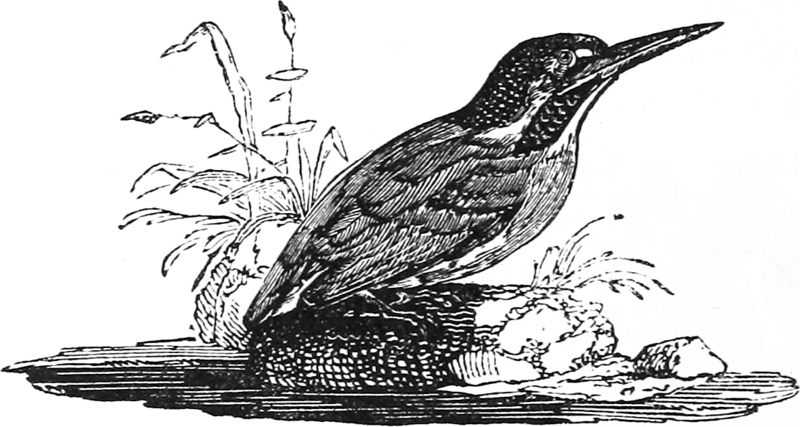
\includegraphics[scale=0.35]{images/Alycon.png}
        \end{figure}
        \vspace{0.5cm}
        \Huge
        \textbf{\textsc{Matematyka Dyskretna}}
        
        \vspace{0.5cm}
        \Large
        \textsc{Wybrane Dowody}
        
        \normalsize
        
        
        \line(1,0){330}
        
        \vspace{1cm}
        \textit{,,Myślę, że 7 punktów na 20 to nie jest zły wynik''}
        \vspace{1cm}

        \textit{\textsc{Popełnione przez}}\\
        \vspace{5mm}

        \textbf{\textsc{Dziurawy Ponton \\ Załatany Ponton \\ Puchaty Pompon \\ Zatopiony Ponton \\ Tonący Ponton \\ Notnop}}

        \vfill

        Kraków \\
        Anno Domini 2023
        
    \end{center}
    
\end{titlepage}


\tableofcontents
\section*{Licencja}
    \begin{figure}[h]
    	\begin{minipage}[c]{0.25\textwidth}
    		
\includegraphics[width=0.7\textwidth]{images/licencja.png}
    	\end{minipage}\hfill
    	\begin{minipage}[c]{0.75\textwidth}
    		\caption*{
    			Ten utwór jest dostępny na 
    			\href{https://creativecommons.org/licenses/by-sa/4.0/}{licencji Creative Commons Uznanie autorstwa
    			na tych samych warunkach 4.0 Międzynarodowe.}
    		}
    	\end{minipage}
    \end{figure}

% Actual content
\mainmatter

\chapter{Kombinatoryka}
 % Żeby nie było syfu to kolejne sekcje dodajemy do chapters/
% A potem includujemy za pomocą \input{chapters/...}

% Używamy \( \) i \[ \] zamiast dolarów -- tak jak się robi w LaTeXu


\documentclass[12pt, a4paper, polish, openany]{book}

% Please, let's familiarize ourselves with notatki.sty and tcs.sty so that we don't reinvent the wheel
\usepackage{notatki}

\fancyhead[L]{\textbf{\textit{MD}}}
\author{
}
\title{TCS and shitposting}


\begin{document}

% Front page and table of contents
\frontmatter

\input{titlepage}

\tableofcontents
\input{license}

% Actual content
\mainmatter

\chapter{Kombinatoryka}
\input{chapters/combinatorics/main}

\chapter{Zasada włączeń i wyłączeń}
\input{chapters/exclusion-inclusion/main}

\chapter{Posety}
\input{chapters/posets/main}

\chapter{Twierdzenie Ramseya}
\input{chapters/ramsey/main}

\chapter{Funkcje tworzące}
\input{chapters/generating_functions/main}

\chapter{Przepływy}
\input{chapters/flows/main}

\chapter{Skojarzenia}
\input{chapters/matchings/main}

\chapter{Kolorowanie grafów}
\input{chapters/graph-coloring/main}

\chapter{Grafy, ale nie kolorowanie}
\input{chapters/graph-misc/main}

\end{document}

\chapter{Zasada włączeń i wyłączeń}
 % Żeby nie było syfu to kolejne sekcje dodajemy do chapters/
% A potem includujemy za pomocą \input{chapters/...}

% Używamy \( \) i \[ \] zamiast dolarów -- tak jak się robi w LaTeXu


\documentclass[12pt, a4paper, polish, openany]{book}

% Please, let's familiarize ourselves with notatki.sty and tcs.sty so that we don't reinvent the wheel
\usepackage{notatki}

\fancyhead[L]{\textbf{\textit{MD}}}
\author{
}
\title{TCS and shitposting}


\begin{document}

% Front page and table of contents
\frontmatter

\input{titlepage}

\tableofcontents
\input{license}

% Actual content
\mainmatter

\chapter{Kombinatoryka}
\input{chapters/combinatorics/main}

\chapter{Zasada włączeń i wyłączeń}
\input{chapters/exclusion-inclusion/main}

\chapter{Posety}
\input{chapters/posets/main}

\chapter{Twierdzenie Ramseya}
\input{chapters/ramsey/main}

\chapter{Funkcje tworzące}
\input{chapters/generating_functions/main}

\chapter{Przepływy}
\input{chapters/flows/main}

\chapter{Skojarzenia}
\input{chapters/matchings/main}

\chapter{Kolorowanie grafów}
\input{chapters/graph-coloring/main}

\chapter{Grafy, ale nie kolorowanie}
\input{chapters/graph-misc/main}

\end{document}

\chapter{Posety}
 % Żeby nie było syfu to kolejne sekcje dodajemy do chapters/
% A potem includujemy za pomocą \input{chapters/...}

% Używamy \( \) i \[ \] zamiast dolarów -- tak jak się robi w LaTeXu


\documentclass[12pt, a4paper, polish, openany]{book}

% Please, let's familiarize ourselves with notatki.sty and tcs.sty so that we don't reinvent the wheel
\usepackage{notatki}

\fancyhead[L]{\textbf{\textit{MD}}}
\author{
}
\title{TCS and shitposting}


\begin{document}

% Front page and table of contents
\frontmatter

\input{titlepage}

\tableofcontents
\input{license}

% Actual content
\mainmatter

\chapter{Kombinatoryka}
\input{chapters/combinatorics/main}

\chapter{Zasada włączeń i wyłączeń}
\input{chapters/exclusion-inclusion/main}

\chapter{Posety}
\input{chapters/posets/main}

\chapter{Twierdzenie Ramseya}
\input{chapters/ramsey/main}

\chapter{Funkcje tworzące}
\input{chapters/generating_functions/main}

\chapter{Przepływy}
\input{chapters/flows/main}

\chapter{Skojarzenia}
\input{chapters/matchings/main}

\chapter{Kolorowanie grafów}
\input{chapters/graph-coloring/main}

\chapter{Grafy, ale nie kolorowanie}
\input{chapters/graph-misc/main}

\end{document}

\chapter{Twierdzenie Ramseya}
 % Żeby nie było syfu to kolejne sekcje dodajemy do chapters/
% A potem includujemy za pomocą \input{chapters/...}

% Używamy \( \) i \[ \] zamiast dolarów -- tak jak się robi w LaTeXu


\documentclass[12pt, a4paper, polish, openany]{book}

% Please, let's familiarize ourselves with notatki.sty and tcs.sty so that we don't reinvent the wheel
\usepackage{notatki}

\fancyhead[L]{\textbf{\textit{MD}}}
\author{
}
\title{TCS and shitposting}


\begin{document}

% Front page and table of contents
\frontmatter

\input{titlepage}

\tableofcontents
\input{license}

% Actual content
\mainmatter

\chapter{Kombinatoryka}
\input{chapters/combinatorics/main}

\chapter{Zasada włączeń i wyłączeń}
\input{chapters/exclusion-inclusion/main}

\chapter{Posety}
\input{chapters/posets/main}

\chapter{Twierdzenie Ramseya}
\input{chapters/ramsey/main}

\chapter{Funkcje tworzące}
\input{chapters/generating_functions/main}

\chapter{Przepływy}
\input{chapters/flows/main}

\chapter{Skojarzenia}
\input{chapters/matchings/main}

\chapter{Kolorowanie grafów}
\input{chapters/graph-coloring/main}

\chapter{Grafy, ale nie kolorowanie}
\input{chapters/graph-misc/main}

\end{document}

\chapter{Funkcje tworzące}
 % Żeby nie było syfu to kolejne sekcje dodajemy do chapters/
% A potem includujemy za pomocą \input{chapters/...}

% Używamy \( \) i \[ \] zamiast dolarów -- tak jak się robi w LaTeXu


\documentclass[12pt, a4paper, polish, openany]{book}

% Please, let's familiarize ourselves with notatki.sty and tcs.sty so that we don't reinvent the wheel
\usepackage{notatki}

\fancyhead[L]{\textbf{\textit{MD}}}
\author{
}
\title{TCS and shitposting}


\begin{document}

% Front page and table of contents
\frontmatter

\input{titlepage}

\tableofcontents
\input{license}

% Actual content
\mainmatter

\chapter{Kombinatoryka}
\input{chapters/combinatorics/main}

\chapter{Zasada włączeń i wyłączeń}
\input{chapters/exclusion-inclusion/main}

\chapter{Posety}
\input{chapters/posets/main}

\chapter{Twierdzenie Ramseya}
\input{chapters/ramsey/main}

\chapter{Funkcje tworzące}
\input{chapters/generating_functions/main}

\chapter{Przepływy}
\input{chapters/flows/main}

\chapter{Skojarzenia}
\input{chapters/matchings/main}

\chapter{Kolorowanie grafów}
\input{chapters/graph-coloring/main}

\chapter{Grafy, ale nie kolorowanie}
\input{chapters/graph-misc/main}

\end{document}

\chapter{Przepływy}
 % Żeby nie było syfu to kolejne sekcje dodajemy do chapters/
% A potem includujemy za pomocą \input{chapters/...}

% Używamy \( \) i \[ \] zamiast dolarów -- tak jak się robi w LaTeXu


\documentclass[12pt, a4paper, polish, openany]{book}

% Please, let's familiarize ourselves with notatki.sty and tcs.sty so that we don't reinvent the wheel
\usepackage{notatki}

\fancyhead[L]{\textbf{\textit{MD}}}
\author{
}
\title{TCS and shitposting}


\begin{document}

% Front page and table of contents
\frontmatter

\input{titlepage}

\tableofcontents
\input{license}

% Actual content
\mainmatter

\chapter{Kombinatoryka}
\input{chapters/combinatorics/main}

\chapter{Zasada włączeń i wyłączeń}
\input{chapters/exclusion-inclusion/main}

\chapter{Posety}
\input{chapters/posets/main}

\chapter{Twierdzenie Ramseya}
\input{chapters/ramsey/main}

\chapter{Funkcje tworzące}
\input{chapters/generating_functions/main}

\chapter{Przepływy}
\input{chapters/flows/main}

\chapter{Skojarzenia}
\input{chapters/matchings/main}

\chapter{Kolorowanie grafów}
\input{chapters/graph-coloring/main}

\chapter{Grafy, ale nie kolorowanie}
\input{chapters/graph-misc/main}

\end{document}

\chapter{Skojarzenia}
 % Żeby nie było syfu to kolejne sekcje dodajemy do chapters/
% A potem includujemy za pomocą \input{chapters/...}

% Używamy \( \) i \[ \] zamiast dolarów -- tak jak się robi w LaTeXu


\documentclass[12pt, a4paper, polish, openany]{book}

% Please, let's familiarize ourselves with notatki.sty and tcs.sty so that we don't reinvent the wheel
\usepackage{notatki}

\fancyhead[L]{\textbf{\textit{MD}}}
\author{
}
\title{TCS and shitposting}


\begin{document}

% Front page and table of contents
\frontmatter

\input{titlepage}

\tableofcontents
\input{license}

% Actual content
\mainmatter

\chapter{Kombinatoryka}
\input{chapters/combinatorics/main}

\chapter{Zasada włączeń i wyłączeń}
\input{chapters/exclusion-inclusion/main}

\chapter{Posety}
\input{chapters/posets/main}

\chapter{Twierdzenie Ramseya}
\input{chapters/ramsey/main}

\chapter{Funkcje tworzące}
\input{chapters/generating_functions/main}

\chapter{Przepływy}
\input{chapters/flows/main}

\chapter{Skojarzenia}
\input{chapters/matchings/main}

\chapter{Kolorowanie grafów}
\input{chapters/graph-coloring/main}

\chapter{Grafy, ale nie kolorowanie}
\input{chapters/graph-misc/main}

\end{document}

\chapter{Kolorowanie grafów}
 % Żeby nie było syfu to kolejne sekcje dodajemy do chapters/
% A potem includujemy za pomocą \input{chapters/...}

% Używamy \( \) i \[ \] zamiast dolarów -- tak jak się robi w LaTeXu


\documentclass[12pt, a4paper, polish, openany]{book}

% Please, let's familiarize ourselves with notatki.sty and tcs.sty so that we don't reinvent the wheel
\usepackage{notatki}

\fancyhead[L]{\textbf{\textit{MD}}}
\author{
}
\title{TCS and shitposting}


\begin{document}

% Front page and table of contents
\frontmatter

\input{titlepage}

\tableofcontents
\input{license}

% Actual content
\mainmatter

\chapter{Kombinatoryka}
\input{chapters/combinatorics/main}

\chapter{Zasada włączeń i wyłączeń}
\input{chapters/exclusion-inclusion/main}

\chapter{Posety}
\input{chapters/posets/main}

\chapter{Twierdzenie Ramseya}
\input{chapters/ramsey/main}

\chapter{Funkcje tworzące}
\input{chapters/generating_functions/main}

\chapter{Przepływy}
\input{chapters/flows/main}

\chapter{Skojarzenia}
\input{chapters/matchings/main}

\chapter{Kolorowanie grafów}
\input{chapters/graph-coloring/main}

\chapter{Grafy, ale nie kolorowanie}
\input{chapters/graph-misc/main}

\end{document}

\chapter{Grafy, ale nie kolorowanie}
 % Żeby nie było syfu to kolejne sekcje dodajemy do chapters/
% A potem includujemy za pomocą \input{chapters/...}

% Używamy \( \) i \[ \] zamiast dolarów -- tak jak się robi w LaTeXu


\documentclass[12pt, a4paper, polish, openany]{book}

% Please, let's familiarize ourselves with notatki.sty and tcs.sty so that we don't reinvent the wheel
\usepackage{notatki}

\fancyhead[L]{\textbf{\textit{MD}}}
\author{
}
\title{TCS and shitposting}


\begin{document}

% Front page and table of contents
\frontmatter

\input{titlepage}

\tableofcontents
\input{license}

% Actual content
\mainmatter

\chapter{Kombinatoryka}
\input{chapters/combinatorics/main}

\chapter{Zasada włączeń i wyłączeń}
\input{chapters/exclusion-inclusion/main}

\chapter{Posety}
\input{chapters/posets/main}

\chapter{Twierdzenie Ramseya}
\input{chapters/ramsey/main}

\chapter{Funkcje tworzące}
\input{chapters/generating_functions/main}

\chapter{Przepływy}
\input{chapters/flows/main}

\chapter{Skojarzenia}
\input{chapters/matchings/main}

\chapter{Kolorowanie grafów}
\input{chapters/graph-coloring/main}

\chapter{Grafy, ale nie kolorowanie}
\input{chapters/graph-misc/main}

\end{document}

\end{document}

\chapter{Kolorowanie grafów}
 % Żeby nie było syfu to kolejne sekcje dodajemy do chapters/
% A potem includujemy za pomocą \input{chapters/...}

% Używamy \( \) i \[ \] zamiast dolarów -- tak jak się robi w LaTeXu


\documentclass[12pt, a4paper, polish, openany]{book}

% Please, let's familiarize ourselves with notatki.sty and tcs.sty so that we don't reinvent the wheel
\usepackage{notatki}

\fancyhead[L]{\textbf{\textit{MD}}}
\author{
}
\title{TCS and shitposting}


\begin{document}

% Front page and table of contents
\frontmatter

\begin{titlepage} 

    \begin{center}
         \begin{figure}[h]
            \centering
            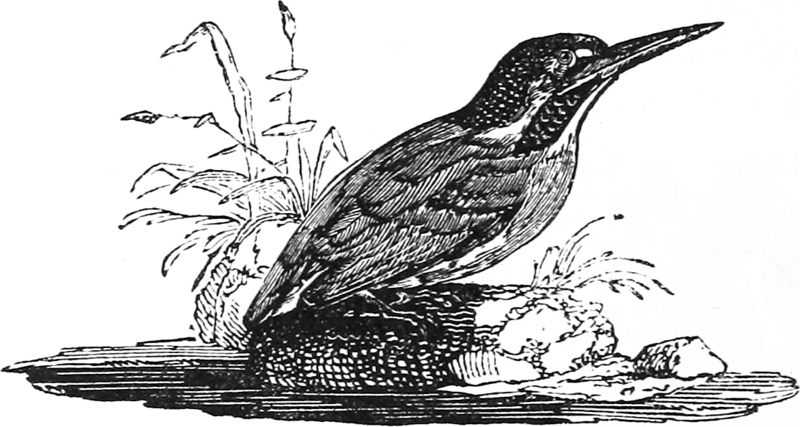
\includegraphics[scale=0.35]{images/Alycon.png}
        \end{figure}
        \vspace{0.5cm}
        \Huge
        \textbf{\textsc{Matematyka Dyskretna}}
        
        \vspace{0.5cm}
        \Large
        \textsc{Wybrane Dowody}
        
        \normalsize
        
        
        \line(1,0){330}
        
        \vspace{1cm}
        \textit{,,Myślę, że 7 punktów na 20 to nie jest zły wynik''}
        \vspace{1cm}

        \textit{\textsc{Popełnione przez}}\\
        \vspace{5mm}

        \textbf{\textsc{Dziurawy Ponton \\ Załatany Ponton \\ Puchaty Pompon \\ Zatopiony Ponton \\ Tonący Ponton \\ Notnop}}

        \vfill

        Kraków \\
        Anno Domini 2023
        
    \end{center}
    
\end{titlepage}


\tableofcontents
\section*{Licencja}
    \begin{figure}[h]
    	\begin{minipage}[c]{0.25\textwidth}
    		
\includegraphics[width=0.7\textwidth]{images/licencja.png}
    	\end{minipage}\hfill
    	\begin{minipage}[c]{0.75\textwidth}
    		\caption*{
    			Ten utwór jest dostępny na 
    			\href{https://creativecommons.org/licenses/by-sa/4.0/}{licencji Creative Commons Uznanie autorstwa
    			na tych samych warunkach 4.0 Międzynarodowe.}
    		}
    	\end{minipage}
    \end{figure}

% Actual content
\mainmatter

\chapter{Kombinatoryka}
 % Żeby nie było syfu to kolejne sekcje dodajemy do chapters/
% A potem includujemy za pomocą \input{chapters/...}

% Używamy \( \) i \[ \] zamiast dolarów -- tak jak się robi w LaTeXu


\documentclass[12pt, a4paper, polish, openany]{book}

% Please, let's familiarize ourselves with notatki.sty and tcs.sty so that we don't reinvent the wheel
\usepackage{notatki}

\fancyhead[L]{\textbf{\textit{MD}}}
\author{
}
\title{TCS and shitposting}


\begin{document}

% Front page and table of contents
\frontmatter

\input{titlepage}

\tableofcontents
\input{license}

% Actual content
\mainmatter

\chapter{Kombinatoryka}
\input{chapters/combinatorics/main}

\chapter{Zasada włączeń i wyłączeń}
\input{chapters/exclusion-inclusion/main}

\chapter{Posety}
\input{chapters/posets/main}

\chapter{Twierdzenie Ramseya}
\input{chapters/ramsey/main}

\chapter{Funkcje tworzące}
\input{chapters/generating_functions/main}

\chapter{Przepływy}
\input{chapters/flows/main}

\chapter{Skojarzenia}
\input{chapters/matchings/main}

\chapter{Kolorowanie grafów}
\input{chapters/graph-coloring/main}

\chapter{Grafy, ale nie kolorowanie}
\input{chapters/graph-misc/main}

\end{document}

\chapter{Zasada włączeń i wyłączeń}
 % Żeby nie było syfu to kolejne sekcje dodajemy do chapters/
% A potem includujemy za pomocą \input{chapters/...}

% Używamy \( \) i \[ \] zamiast dolarów -- tak jak się robi w LaTeXu


\documentclass[12pt, a4paper, polish, openany]{book}

% Please, let's familiarize ourselves with notatki.sty and tcs.sty so that we don't reinvent the wheel
\usepackage{notatki}

\fancyhead[L]{\textbf{\textit{MD}}}
\author{
}
\title{TCS and shitposting}


\begin{document}

% Front page and table of contents
\frontmatter

\input{titlepage}

\tableofcontents
\input{license}

% Actual content
\mainmatter

\chapter{Kombinatoryka}
\input{chapters/combinatorics/main}

\chapter{Zasada włączeń i wyłączeń}
\input{chapters/exclusion-inclusion/main}

\chapter{Posety}
\input{chapters/posets/main}

\chapter{Twierdzenie Ramseya}
\input{chapters/ramsey/main}

\chapter{Funkcje tworzące}
\input{chapters/generating_functions/main}

\chapter{Przepływy}
\input{chapters/flows/main}

\chapter{Skojarzenia}
\input{chapters/matchings/main}

\chapter{Kolorowanie grafów}
\input{chapters/graph-coloring/main}

\chapter{Grafy, ale nie kolorowanie}
\input{chapters/graph-misc/main}

\end{document}

\chapter{Posety}
 % Żeby nie było syfu to kolejne sekcje dodajemy do chapters/
% A potem includujemy za pomocą \input{chapters/...}

% Używamy \( \) i \[ \] zamiast dolarów -- tak jak się robi w LaTeXu


\documentclass[12pt, a4paper, polish, openany]{book}

% Please, let's familiarize ourselves with notatki.sty and tcs.sty so that we don't reinvent the wheel
\usepackage{notatki}

\fancyhead[L]{\textbf{\textit{MD}}}
\author{
}
\title{TCS and shitposting}


\begin{document}

% Front page and table of contents
\frontmatter

\input{titlepage}

\tableofcontents
\input{license}

% Actual content
\mainmatter

\chapter{Kombinatoryka}
\input{chapters/combinatorics/main}

\chapter{Zasada włączeń i wyłączeń}
\input{chapters/exclusion-inclusion/main}

\chapter{Posety}
\input{chapters/posets/main}

\chapter{Twierdzenie Ramseya}
\input{chapters/ramsey/main}

\chapter{Funkcje tworzące}
\input{chapters/generating_functions/main}

\chapter{Przepływy}
\input{chapters/flows/main}

\chapter{Skojarzenia}
\input{chapters/matchings/main}

\chapter{Kolorowanie grafów}
\input{chapters/graph-coloring/main}

\chapter{Grafy, ale nie kolorowanie}
\input{chapters/graph-misc/main}

\end{document}

\chapter{Twierdzenie Ramseya}
 % Żeby nie było syfu to kolejne sekcje dodajemy do chapters/
% A potem includujemy za pomocą \input{chapters/...}

% Używamy \( \) i \[ \] zamiast dolarów -- tak jak się robi w LaTeXu


\documentclass[12pt, a4paper, polish, openany]{book}

% Please, let's familiarize ourselves with notatki.sty and tcs.sty so that we don't reinvent the wheel
\usepackage{notatki}

\fancyhead[L]{\textbf{\textit{MD}}}
\author{
}
\title{TCS and shitposting}


\begin{document}

% Front page and table of contents
\frontmatter

\input{titlepage}

\tableofcontents
\input{license}

% Actual content
\mainmatter

\chapter{Kombinatoryka}
\input{chapters/combinatorics/main}

\chapter{Zasada włączeń i wyłączeń}
\input{chapters/exclusion-inclusion/main}

\chapter{Posety}
\input{chapters/posets/main}

\chapter{Twierdzenie Ramseya}
\input{chapters/ramsey/main}

\chapter{Funkcje tworzące}
\input{chapters/generating_functions/main}

\chapter{Przepływy}
\input{chapters/flows/main}

\chapter{Skojarzenia}
\input{chapters/matchings/main}

\chapter{Kolorowanie grafów}
\input{chapters/graph-coloring/main}

\chapter{Grafy, ale nie kolorowanie}
\input{chapters/graph-misc/main}

\end{document}

\chapter{Funkcje tworzące}
 % Żeby nie było syfu to kolejne sekcje dodajemy do chapters/
% A potem includujemy za pomocą \input{chapters/...}

% Używamy \( \) i \[ \] zamiast dolarów -- tak jak się robi w LaTeXu


\documentclass[12pt, a4paper, polish, openany]{book}

% Please, let's familiarize ourselves with notatki.sty and tcs.sty so that we don't reinvent the wheel
\usepackage{notatki}

\fancyhead[L]{\textbf{\textit{MD}}}
\author{
}
\title{TCS and shitposting}


\begin{document}

% Front page and table of contents
\frontmatter

\input{titlepage}

\tableofcontents
\input{license}

% Actual content
\mainmatter

\chapter{Kombinatoryka}
\input{chapters/combinatorics/main}

\chapter{Zasada włączeń i wyłączeń}
\input{chapters/exclusion-inclusion/main}

\chapter{Posety}
\input{chapters/posets/main}

\chapter{Twierdzenie Ramseya}
\input{chapters/ramsey/main}

\chapter{Funkcje tworzące}
\input{chapters/generating_functions/main}

\chapter{Przepływy}
\input{chapters/flows/main}

\chapter{Skojarzenia}
\input{chapters/matchings/main}

\chapter{Kolorowanie grafów}
\input{chapters/graph-coloring/main}

\chapter{Grafy, ale nie kolorowanie}
\input{chapters/graph-misc/main}

\end{document}

\chapter{Przepływy}
 % Żeby nie było syfu to kolejne sekcje dodajemy do chapters/
% A potem includujemy za pomocą \input{chapters/...}

% Używamy \( \) i \[ \] zamiast dolarów -- tak jak się robi w LaTeXu


\documentclass[12pt, a4paper, polish, openany]{book}

% Please, let's familiarize ourselves with notatki.sty and tcs.sty so that we don't reinvent the wheel
\usepackage{notatki}

\fancyhead[L]{\textbf{\textit{MD}}}
\author{
}
\title{TCS and shitposting}


\begin{document}

% Front page and table of contents
\frontmatter

\input{titlepage}

\tableofcontents
\input{license}

% Actual content
\mainmatter

\chapter{Kombinatoryka}
\input{chapters/combinatorics/main}

\chapter{Zasada włączeń i wyłączeń}
\input{chapters/exclusion-inclusion/main}

\chapter{Posety}
\input{chapters/posets/main}

\chapter{Twierdzenie Ramseya}
\input{chapters/ramsey/main}

\chapter{Funkcje tworzące}
\input{chapters/generating_functions/main}

\chapter{Przepływy}
\input{chapters/flows/main}

\chapter{Skojarzenia}
\input{chapters/matchings/main}

\chapter{Kolorowanie grafów}
\input{chapters/graph-coloring/main}

\chapter{Grafy, ale nie kolorowanie}
\input{chapters/graph-misc/main}

\end{document}

\chapter{Skojarzenia}
 % Żeby nie było syfu to kolejne sekcje dodajemy do chapters/
% A potem includujemy za pomocą \input{chapters/...}

% Używamy \( \) i \[ \] zamiast dolarów -- tak jak się robi w LaTeXu


\documentclass[12pt, a4paper, polish, openany]{book}

% Please, let's familiarize ourselves with notatki.sty and tcs.sty so that we don't reinvent the wheel
\usepackage{notatki}

\fancyhead[L]{\textbf{\textit{MD}}}
\author{
}
\title{TCS and shitposting}


\begin{document}

% Front page and table of contents
\frontmatter

\input{titlepage}

\tableofcontents
\input{license}

% Actual content
\mainmatter

\chapter{Kombinatoryka}
\input{chapters/combinatorics/main}

\chapter{Zasada włączeń i wyłączeń}
\input{chapters/exclusion-inclusion/main}

\chapter{Posety}
\input{chapters/posets/main}

\chapter{Twierdzenie Ramseya}
\input{chapters/ramsey/main}

\chapter{Funkcje tworzące}
\input{chapters/generating_functions/main}

\chapter{Przepływy}
\input{chapters/flows/main}

\chapter{Skojarzenia}
\input{chapters/matchings/main}

\chapter{Kolorowanie grafów}
\input{chapters/graph-coloring/main}

\chapter{Grafy, ale nie kolorowanie}
\input{chapters/graph-misc/main}

\end{document}

\chapter{Kolorowanie grafów}
 % Żeby nie było syfu to kolejne sekcje dodajemy do chapters/
% A potem includujemy za pomocą \input{chapters/...}

% Używamy \( \) i \[ \] zamiast dolarów -- tak jak się robi w LaTeXu


\documentclass[12pt, a4paper, polish, openany]{book}

% Please, let's familiarize ourselves with notatki.sty and tcs.sty so that we don't reinvent the wheel
\usepackage{notatki}

\fancyhead[L]{\textbf{\textit{MD}}}
\author{
}
\title{TCS and shitposting}


\begin{document}

% Front page and table of contents
\frontmatter

\input{titlepage}

\tableofcontents
\input{license}

% Actual content
\mainmatter

\chapter{Kombinatoryka}
\input{chapters/combinatorics/main}

\chapter{Zasada włączeń i wyłączeń}
\input{chapters/exclusion-inclusion/main}

\chapter{Posety}
\input{chapters/posets/main}

\chapter{Twierdzenie Ramseya}
\input{chapters/ramsey/main}

\chapter{Funkcje tworzące}
\input{chapters/generating_functions/main}

\chapter{Przepływy}
\input{chapters/flows/main}

\chapter{Skojarzenia}
\input{chapters/matchings/main}

\chapter{Kolorowanie grafów}
\input{chapters/graph-coloring/main}

\chapter{Grafy, ale nie kolorowanie}
\input{chapters/graph-misc/main}

\end{document}

\chapter{Grafy, ale nie kolorowanie}
 % Żeby nie było syfu to kolejne sekcje dodajemy do chapters/
% A potem includujemy za pomocą \input{chapters/...}

% Używamy \( \) i \[ \] zamiast dolarów -- tak jak się robi w LaTeXu


\documentclass[12pt, a4paper, polish, openany]{book}

% Please, let's familiarize ourselves with notatki.sty and tcs.sty so that we don't reinvent the wheel
\usepackage{notatki}

\fancyhead[L]{\textbf{\textit{MD}}}
\author{
}
\title{TCS and shitposting}


\begin{document}

% Front page and table of contents
\frontmatter

\input{titlepage}

\tableofcontents
\input{license}

% Actual content
\mainmatter

\chapter{Kombinatoryka}
\input{chapters/combinatorics/main}

\chapter{Zasada włączeń i wyłączeń}
\input{chapters/exclusion-inclusion/main}

\chapter{Posety}
\input{chapters/posets/main}

\chapter{Twierdzenie Ramseya}
\input{chapters/ramsey/main}

\chapter{Funkcje tworzące}
\input{chapters/generating_functions/main}

\chapter{Przepływy}
\input{chapters/flows/main}

\chapter{Skojarzenia}
\input{chapters/matchings/main}

\chapter{Kolorowanie grafów}
\input{chapters/graph-coloring/main}

\chapter{Grafy, ale nie kolorowanie}
\input{chapters/graph-misc/main}

\end{document}

\end{document}

\chapter{Grafy, ale nie kolorowanie}
 % Żeby nie było syfu to kolejne sekcje dodajemy do chapters/
% A potem includujemy za pomocą \input{chapters/...}

% Używamy \( \) i \[ \] zamiast dolarów -- tak jak się robi w LaTeXu


\documentclass[12pt, a4paper, polish, openany]{book}

% Please, let's familiarize ourselves with notatki.sty and tcs.sty so that we don't reinvent the wheel
\usepackage{notatki}

\fancyhead[L]{\textbf{\textit{MD}}}
\author{
}
\title{TCS and shitposting}


\begin{document}

% Front page and table of contents
\frontmatter

\begin{titlepage} 

    \begin{center}
         \begin{figure}[h]
            \centering
            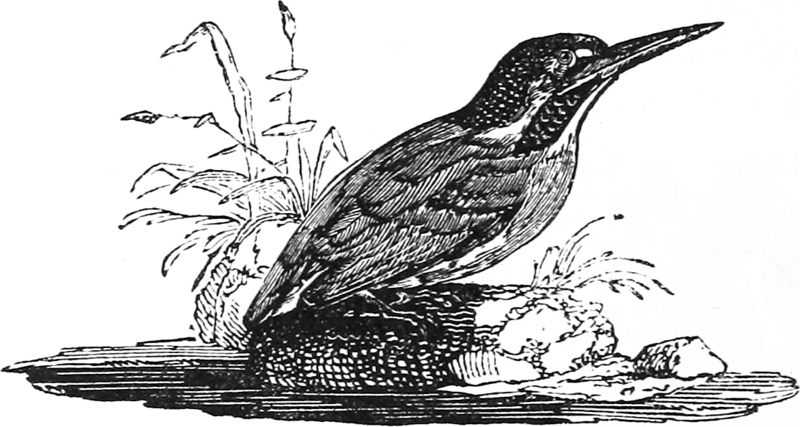
\includegraphics[scale=0.35]{images/Alycon.png}
        \end{figure}
        \vspace{0.5cm}
        \Huge
        \textbf{\textsc{Matematyka Dyskretna}}
        
        \vspace{0.5cm}
        \Large
        \textsc{Wybrane Dowody}
        
        \normalsize
        
        
        \line(1,0){330}
        
        \vspace{1cm}
        \textit{,,Myślę, że 7 punktów na 20 to nie jest zły wynik''}
        \vspace{1cm}

        \textit{\textsc{Popełnione przez}}\\
        \vspace{5mm}

        \textbf{\textsc{Dziurawy Ponton \\ Załatany Ponton \\ Puchaty Pompon \\ Zatopiony Ponton \\ Tonący Ponton \\ Notnop}}

        \vfill

        Kraków \\
        Anno Domini 2023
        
    \end{center}
    
\end{titlepage}


\tableofcontents
\section*{Licencja}
    \begin{figure}[h]
    	\begin{minipage}[c]{0.25\textwidth}
    		
\includegraphics[width=0.7\textwidth]{images/licencja.png}
    	\end{minipage}\hfill
    	\begin{minipage}[c]{0.75\textwidth}
    		\caption*{
    			Ten utwór jest dostępny na 
    			\href{https://creativecommons.org/licenses/by-sa/4.0/}{licencji Creative Commons Uznanie autorstwa
    			na tych samych warunkach 4.0 Międzynarodowe.}
    		}
    	\end{minipage}
    \end{figure}

% Actual content
\mainmatter

\chapter{Kombinatoryka}
 % Żeby nie było syfu to kolejne sekcje dodajemy do chapters/
% A potem includujemy za pomocą \input{chapters/...}

% Używamy \( \) i \[ \] zamiast dolarów -- tak jak się robi w LaTeXu


\documentclass[12pt, a4paper, polish, openany]{book}

% Please, let's familiarize ourselves with notatki.sty and tcs.sty so that we don't reinvent the wheel
\usepackage{notatki}

\fancyhead[L]{\textbf{\textit{MD}}}
\author{
}
\title{TCS and shitposting}


\begin{document}

% Front page and table of contents
\frontmatter

\input{titlepage}

\tableofcontents
\input{license}

% Actual content
\mainmatter

\chapter{Kombinatoryka}
\input{chapters/combinatorics/main}

\chapter{Zasada włączeń i wyłączeń}
\input{chapters/exclusion-inclusion/main}

\chapter{Posety}
\input{chapters/posets/main}

\chapter{Twierdzenie Ramseya}
\input{chapters/ramsey/main}

\chapter{Funkcje tworzące}
\input{chapters/generating_functions/main}

\chapter{Przepływy}
\input{chapters/flows/main}

\chapter{Skojarzenia}
\input{chapters/matchings/main}

\chapter{Kolorowanie grafów}
\input{chapters/graph-coloring/main}

\chapter{Grafy, ale nie kolorowanie}
\input{chapters/graph-misc/main}

\end{document}

\chapter{Zasada włączeń i wyłączeń}
 % Żeby nie było syfu to kolejne sekcje dodajemy do chapters/
% A potem includujemy za pomocą \input{chapters/...}

% Używamy \( \) i \[ \] zamiast dolarów -- tak jak się robi w LaTeXu


\documentclass[12pt, a4paper, polish, openany]{book}

% Please, let's familiarize ourselves with notatki.sty and tcs.sty so that we don't reinvent the wheel
\usepackage{notatki}

\fancyhead[L]{\textbf{\textit{MD}}}
\author{
}
\title{TCS and shitposting}


\begin{document}

% Front page and table of contents
\frontmatter

\input{titlepage}

\tableofcontents
\input{license}

% Actual content
\mainmatter

\chapter{Kombinatoryka}
\input{chapters/combinatorics/main}

\chapter{Zasada włączeń i wyłączeń}
\input{chapters/exclusion-inclusion/main}

\chapter{Posety}
\input{chapters/posets/main}

\chapter{Twierdzenie Ramseya}
\input{chapters/ramsey/main}

\chapter{Funkcje tworzące}
\input{chapters/generating_functions/main}

\chapter{Przepływy}
\input{chapters/flows/main}

\chapter{Skojarzenia}
\input{chapters/matchings/main}

\chapter{Kolorowanie grafów}
\input{chapters/graph-coloring/main}

\chapter{Grafy, ale nie kolorowanie}
\input{chapters/graph-misc/main}

\end{document}

\chapter{Posety}
 % Żeby nie było syfu to kolejne sekcje dodajemy do chapters/
% A potem includujemy za pomocą \input{chapters/...}

% Używamy \( \) i \[ \] zamiast dolarów -- tak jak się robi w LaTeXu


\documentclass[12pt, a4paper, polish, openany]{book}

% Please, let's familiarize ourselves with notatki.sty and tcs.sty so that we don't reinvent the wheel
\usepackage{notatki}

\fancyhead[L]{\textbf{\textit{MD}}}
\author{
}
\title{TCS and shitposting}


\begin{document}

% Front page and table of contents
\frontmatter

\input{titlepage}

\tableofcontents
\input{license}

% Actual content
\mainmatter

\chapter{Kombinatoryka}
\input{chapters/combinatorics/main}

\chapter{Zasada włączeń i wyłączeń}
\input{chapters/exclusion-inclusion/main}

\chapter{Posety}
\input{chapters/posets/main}

\chapter{Twierdzenie Ramseya}
\input{chapters/ramsey/main}

\chapter{Funkcje tworzące}
\input{chapters/generating_functions/main}

\chapter{Przepływy}
\input{chapters/flows/main}

\chapter{Skojarzenia}
\input{chapters/matchings/main}

\chapter{Kolorowanie grafów}
\input{chapters/graph-coloring/main}

\chapter{Grafy, ale nie kolorowanie}
\input{chapters/graph-misc/main}

\end{document}

\chapter{Twierdzenie Ramseya}
 % Żeby nie było syfu to kolejne sekcje dodajemy do chapters/
% A potem includujemy za pomocą \input{chapters/...}

% Używamy \( \) i \[ \] zamiast dolarów -- tak jak się robi w LaTeXu


\documentclass[12pt, a4paper, polish, openany]{book}

% Please, let's familiarize ourselves with notatki.sty and tcs.sty so that we don't reinvent the wheel
\usepackage{notatki}

\fancyhead[L]{\textbf{\textit{MD}}}
\author{
}
\title{TCS and shitposting}


\begin{document}

% Front page and table of contents
\frontmatter

\input{titlepage}

\tableofcontents
\input{license}

% Actual content
\mainmatter

\chapter{Kombinatoryka}
\input{chapters/combinatorics/main}

\chapter{Zasada włączeń i wyłączeń}
\input{chapters/exclusion-inclusion/main}

\chapter{Posety}
\input{chapters/posets/main}

\chapter{Twierdzenie Ramseya}
\input{chapters/ramsey/main}

\chapter{Funkcje tworzące}
\input{chapters/generating_functions/main}

\chapter{Przepływy}
\input{chapters/flows/main}

\chapter{Skojarzenia}
\input{chapters/matchings/main}

\chapter{Kolorowanie grafów}
\input{chapters/graph-coloring/main}

\chapter{Grafy, ale nie kolorowanie}
\input{chapters/graph-misc/main}

\end{document}

\chapter{Funkcje tworzące}
 % Żeby nie było syfu to kolejne sekcje dodajemy do chapters/
% A potem includujemy za pomocą \input{chapters/...}

% Używamy \( \) i \[ \] zamiast dolarów -- tak jak się robi w LaTeXu


\documentclass[12pt, a4paper, polish, openany]{book}

% Please, let's familiarize ourselves with notatki.sty and tcs.sty so that we don't reinvent the wheel
\usepackage{notatki}

\fancyhead[L]{\textbf{\textit{MD}}}
\author{
}
\title{TCS and shitposting}


\begin{document}

% Front page and table of contents
\frontmatter

\input{titlepage}

\tableofcontents
\input{license}

% Actual content
\mainmatter

\chapter{Kombinatoryka}
\input{chapters/combinatorics/main}

\chapter{Zasada włączeń i wyłączeń}
\input{chapters/exclusion-inclusion/main}

\chapter{Posety}
\input{chapters/posets/main}

\chapter{Twierdzenie Ramseya}
\input{chapters/ramsey/main}

\chapter{Funkcje tworzące}
\input{chapters/generating_functions/main}

\chapter{Przepływy}
\input{chapters/flows/main}

\chapter{Skojarzenia}
\input{chapters/matchings/main}

\chapter{Kolorowanie grafów}
\input{chapters/graph-coloring/main}

\chapter{Grafy, ale nie kolorowanie}
\input{chapters/graph-misc/main}

\end{document}

\chapter{Przepływy}
 % Żeby nie było syfu to kolejne sekcje dodajemy do chapters/
% A potem includujemy za pomocą \input{chapters/...}

% Używamy \( \) i \[ \] zamiast dolarów -- tak jak się robi w LaTeXu


\documentclass[12pt, a4paper, polish, openany]{book}

% Please, let's familiarize ourselves with notatki.sty and tcs.sty so that we don't reinvent the wheel
\usepackage{notatki}

\fancyhead[L]{\textbf{\textit{MD}}}
\author{
}
\title{TCS and shitposting}


\begin{document}

% Front page and table of contents
\frontmatter

\input{titlepage}

\tableofcontents
\input{license}

% Actual content
\mainmatter

\chapter{Kombinatoryka}
\input{chapters/combinatorics/main}

\chapter{Zasada włączeń i wyłączeń}
\input{chapters/exclusion-inclusion/main}

\chapter{Posety}
\input{chapters/posets/main}

\chapter{Twierdzenie Ramseya}
\input{chapters/ramsey/main}

\chapter{Funkcje tworzące}
\input{chapters/generating_functions/main}

\chapter{Przepływy}
\input{chapters/flows/main}

\chapter{Skojarzenia}
\input{chapters/matchings/main}

\chapter{Kolorowanie grafów}
\input{chapters/graph-coloring/main}

\chapter{Grafy, ale nie kolorowanie}
\input{chapters/graph-misc/main}

\end{document}

\chapter{Skojarzenia}
 % Żeby nie było syfu to kolejne sekcje dodajemy do chapters/
% A potem includujemy za pomocą \input{chapters/...}

% Używamy \( \) i \[ \] zamiast dolarów -- tak jak się robi w LaTeXu


\documentclass[12pt, a4paper, polish, openany]{book}

% Please, let's familiarize ourselves with notatki.sty and tcs.sty so that we don't reinvent the wheel
\usepackage{notatki}

\fancyhead[L]{\textbf{\textit{MD}}}
\author{
}
\title{TCS and shitposting}


\begin{document}

% Front page and table of contents
\frontmatter

\input{titlepage}

\tableofcontents
\input{license}

% Actual content
\mainmatter

\chapter{Kombinatoryka}
\input{chapters/combinatorics/main}

\chapter{Zasada włączeń i wyłączeń}
\input{chapters/exclusion-inclusion/main}

\chapter{Posety}
\input{chapters/posets/main}

\chapter{Twierdzenie Ramseya}
\input{chapters/ramsey/main}

\chapter{Funkcje tworzące}
\input{chapters/generating_functions/main}

\chapter{Przepływy}
\input{chapters/flows/main}

\chapter{Skojarzenia}
\input{chapters/matchings/main}

\chapter{Kolorowanie grafów}
\input{chapters/graph-coloring/main}

\chapter{Grafy, ale nie kolorowanie}
\input{chapters/graph-misc/main}

\end{document}

\chapter{Kolorowanie grafów}
 % Żeby nie było syfu to kolejne sekcje dodajemy do chapters/
% A potem includujemy za pomocą \input{chapters/...}

% Używamy \( \) i \[ \] zamiast dolarów -- tak jak się robi w LaTeXu


\documentclass[12pt, a4paper, polish, openany]{book}

% Please, let's familiarize ourselves with notatki.sty and tcs.sty so that we don't reinvent the wheel
\usepackage{notatki}

\fancyhead[L]{\textbf{\textit{MD}}}
\author{
}
\title{TCS and shitposting}


\begin{document}

% Front page and table of contents
\frontmatter

\input{titlepage}

\tableofcontents
\input{license}

% Actual content
\mainmatter

\chapter{Kombinatoryka}
\input{chapters/combinatorics/main}

\chapter{Zasada włączeń i wyłączeń}
\input{chapters/exclusion-inclusion/main}

\chapter{Posety}
\input{chapters/posets/main}

\chapter{Twierdzenie Ramseya}
\input{chapters/ramsey/main}

\chapter{Funkcje tworzące}
\input{chapters/generating_functions/main}

\chapter{Przepływy}
\input{chapters/flows/main}

\chapter{Skojarzenia}
\input{chapters/matchings/main}

\chapter{Kolorowanie grafów}
\input{chapters/graph-coloring/main}

\chapter{Grafy, ale nie kolorowanie}
\input{chapters/graph-misc/main}

\end{document}

\chapter{Grafy, ale nie kolorowanie}
 % Żeby nie było syfu to kolejne sekcje dodajemy do chapters/
% A potem includujemy za pomocą \input{chapters/...}

% Używamy \( \) i \[ \] zamiast dolarów -- tak jak się robi w LaTeXu


\documentclass[12pt, a4paper, polish, openany]{book}

% Please, let's familiarize ourselves with notatki.sty and tcs.sty so that we don't reinvent the wheel
\usepackage{notatki}

\fancyhead[L]{\textbf{\textit{MD}}}
\author{
}
\title{TCS and shitposting}


\begin{document}

% Front page and table of contents
\frontmatter

\input{titlepage}

\tableofcontents
\input{license}

% Actual content
\mainmatter

\chapter{Kombinatoryka}
\input{chapters/combinatorics/main}

\chapter{Zasada włączeń i wyłączeń}
\input{chapters/exclusion-inclusion/main}

\chapter{Posety}
\input{chapters/posets/main}

\chapter{Twierdzenie Ramseya}
\input{chapters/ramsey/main}

\chapter{Funkcje tworzące}
\input{chapters/generating_functions/main}

\chapter{Przepływy}
\input{chapters/flows/main}

\chapter{Skojarzenia}
\input{chapters/matchings/main}

\chapter{Kolorowanie grafów}
\input{chapters/graph-coloring/main}

\chapter{Grafy, ale nie kolorowanie}
\input{chapters/graph-misc/main}

\end{document}

\end{document}

\end{document}

\section{Konstrukcja liczb naturalnych von Neumanna, twierdzenie o~indukcji. Własności liczb naturalnych}
\label{mfi:nat_and_induction}
 % Żeby nie było syfu to kolejne sekcje dodajemy do chapters/
% A potem includujemy za pomocą \input{chapters/...}

% Używamy \( \) i \[ \] zamiast dolarów -- tak jak się robi w LaTeXu


\documentclass[12pt, a4paper, polish, openany]{book}

% Please, let's familiarize ourselves with notatki.sty and tcs.sty so that we don't reinvent the wheel
\usepackage{notatki}

\fancyhead[L]{\textbf{\textit{MD}}}
\author{
}
\title{TCS and shitposting}


\begin{document}

% Front page and table of contents
\frontmatter

\begin{titlepage} 

    \begin{center}
         \begin{figure}[h]
            \centering
            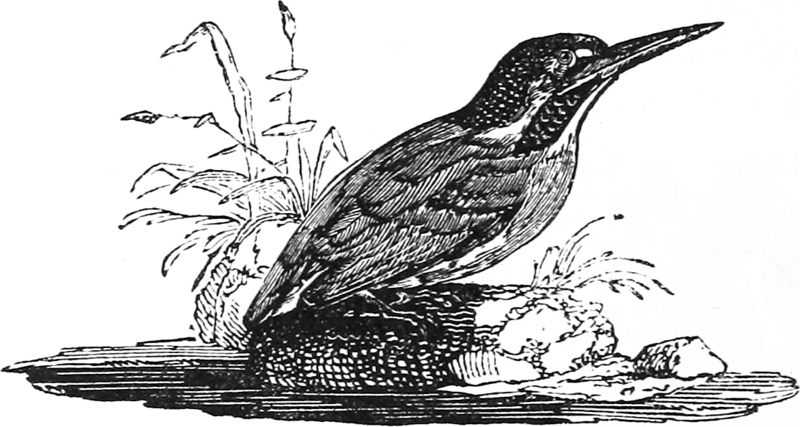
\includegraphics[scale=0.35]{images/Alycon.png}
        \end{figure}
        \vspace{0.5cm}
        \Huge
        \textbf{\textsc{Matematyka Dyskretna}}
        
        \vspace{0.5cm}
        \Large
        \textsc{Wybrane Dowody}
        
        \normalsize
        
        
        \line(1,0){330}
        
        \vspace{1cm}
        \textit{,,Myślę, że 7 punktów na 20 to nie jest zły wynik''}
        \vspace{1cm}

        \textit{\textsc{Popełnione przez}}\\
        \vspace{5mm}

        \textbf{\textsc{Dziurawy Ponton \\ Załatany Ponton \\ Puchaty Pompon \\ Zatopiony Ponton \\ Tonący Ponton \\ Notnop}}

        \vfill

        Kraków \\
        Anno Domini 2023
        
    \end{center}
    
\end{titlepage}


\tableofcontents
\section*{Licencja}
    \begin{figure}[h]
    	\begin{minipage}[c]{0.25\textwidth}
    		
\includegraphics[width=0.7\textwidth]{images/licencja.png}
    	\end{minipage}\hfill
    	\begin{minipage}[c]{0.75\textwidth}
    		\caption*{
    			Ten utwór jest dostępny na 
    			\href{https://creativecommons.org/licenses/by-sa/4.0/}{licencji Creative Commons Uznanie autorstwa
    			na tych samych warunkach 4.0 Międzynarodowe.}
    		}
    	\end{minipage}
    \end{figure}

% Actual content
\mainmatter

\chapter{Kombinatoryka}
 % Żeby nie było syfu to kolejne sekcje dodajemy do chapters/
% A potem includujemy za pomocą \input{chapters/...}

% Używamy \( \) i \[ \] zamiast dolarów -- tak jak się robi w LaTeXu


\documentclass[12pt, a4paper, polish, openany]{book}

% Please, let's familiarize ourselves with notatki.sty and tcs.sty so that we don't reinvent the wheel
\usepackage{notatki}

\fancyhead[L]{\textbf{\textit{MD}}}
\author{
}
\title{TCS and shitposting}


\begin{document}

% Front page and table of contents
\frontmatter

\begin{titlepage} 

    \begin{center}
         \begin{figure}[h]
            \centering
            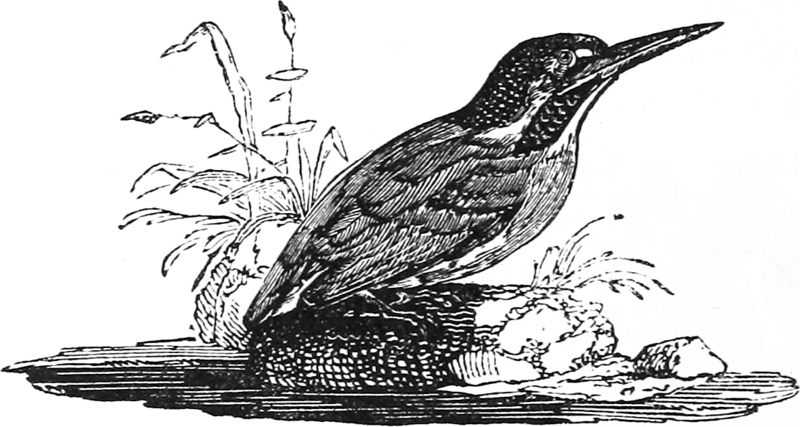
\includegraphics[scale=0.35]{images/Alycon.png}
        \end{figure}
        \vspace{0.5cm}
        \Huge
        \textbf{\textsc{Matematyka Dyskretna}}
        
        \vspace{0.5cm}
        \Large
        \textsc{Wybrane Dowody}
        
        \normalsize
        
        
        \line(1,0){330}
        
        \vspace{1cm}
        \textit{,,Myślę, że 7 punktów na 20 to nie jest zły wynik''}
        \vspace{1cm}

        \textit{\textsc{Popełnione przez}}\\
        \vspace{5mm}

        \textbf{\textsc{Dziurawy Ponton \\ Załatany Ponton \\ Puchaty Pompon \\ Zatopiony Ponton \\ Tonący Ponton \\ Notnop}}

        \vfill

        Kraków \\
        Anno Domini 2023
        
    \end{center}
    
\end{titlepage}


\tableofcontents
\section*{Licencja}
    \begin{figure}[h]
    	\begin{minipage}[c]{0.25\textwidth}
    		
\includegraphics[width=0.7\textwidth]{images/licencja.png}
    	\end{minipage}\hfill
    	\begin{minipage}[c]{0.75\textwidth}
    		\caption*{
    			Ten utwór jest dostępny na 
    			\href{https://creativecommons.org/licenses/by-sa/4.0/}{licencji Creative Commons Uznanie autorstwa
    			na tych samych warunkach 4.0 Międzynarodowe.}
    		}
    	\end{minipage}
    \end{figure}

% Actual content
\mainmatter

\chapter{Kombinatoryka}
 % Żeby nie było syfu to kolejne sekcje dodajemy do chapters/
% A potem includujemy za pomocą \input{chapters/...}

% Używamy \( \) i \[ \] zamiast dolarów -- tak jak się robi w LaTeXu


\documentclass[12pt, a4paper, polish, openany]{book}

% Please, let's familiarize ourselves with notatki.sty and tcs.sty so that we don't reinvent the wheel
\usepackage{notatki}

\fancyhead[L]{\textbf{\textit{MD}}}
\author{
}
\title{TCS and shitposting}


\begin{document}

% Front page and table of contents
\frontmatter

\input{titlepage}

\tableofcontents
\input{license}

% Actual content
\mainmatter

\chapter{Kombinatoryka}
\input{chapters/combinatorics/main}

\chapter{Zasada włączeń i wyłączeń}
\input{chapters/exclusion-inclusion/main}

\chapter{Posety}
\input{chapters/posets/main}

\chapter{Twierdzenie Ramseya}
\input{chapters/ramsey/main}

\chapter{Funkcje tworzące}
\input{chapters/generating_functions/main}

\chapter{Przepływy}
\input{chapters/flows/main}

\chapter{Skojarzenia}
\input{chapters/matchings/main}

\chapter{Kolorowanie grafów}
\input{chapters/graph-coloring/main}

\chapter{Grafy, ale nie kolorowanie}
\input{chapters/graph-misc/main}

\end{document}

\chapter{Zasada włączeń i wyłączeń}
 % Żeby nie było syfu to kolejne sekcje dodajemy do chapters/
% A potem includujemy za pomocą \input{chapters/...}

% Używamy \( \) i \[ \] zamiast dolarów -- tak jak się robi w LaTeXu


\documentclass[12pt, a4paper, polish, openany]{book}

% Please, let's familiarize ourselves with notatki.sty and tcs.sty so that we don't reinvent the wheel
\usepackage{notatki}

\fancyhead[L]{\textbf{\textit{MD}}}
\author{
}
\title{TCS and shitposting}


\begin{document}

% Front page and table of contents
\frontmatter

\input{titlepage}

\tableofcontents
\input{license}

% Actual content
\mainmatter

\chapter{Kombinatoryka}
\input{chapters/combinatorics/main}

\chapter{Zasada włączeń i wyłączeń}
\input{chapters/exclusion-inclusion/main}

\chapter{Posety}
\input{chapters/posets/main}

\chapter{Twierdzenie Ramseya}
\input{chapters/ramsey/main}

\chapter{Funkcje tworzące}
\input{chapters/generating_functions/main}

\chapter{Przepływy}
\input{chapters/flows/main}

\chapter{Skojarzenia}
\input{chapters/matchings/main}

\chapter{Kolorowanie grafów}
\input{chapters/graph-coloring/main}

\chapter{Grafy, ale nie kolorowanie}
\input{chapters/graph-misc/main}

\end{document}

\chapter{Posety}
 % Żeby nie było syfu to kolejne sekcje dodajemy do chapters/
% A potem includujemy za pomocą \input{chapters/...}

% Używamy \( \) i \[ \] zamiast dolarów -- tak jak się robi w LaTeXu


\documentclass[12pt, a4paper, polish, openany]{book}

% Please, let's familiarize ourselves with notatki.sty and tcs.sty so that we don't reinvent the wheel
\usepackage{notatki}

\fancyhead[L]{\textbf{\textit{MD}}}
\author{
}
\title{TCS and shitposting}


\begin{document}

% Front page and table of contents
\frontmatter

\input{titlepage}

\tableofcontents
\input{license}

% Actual content
\mainmatter

\chapter{Kombinatoryka}
\input{chapters/combinatorics/main}

\chapter{Zasada włączeń i wyłączeń}
\input{chapters/exclusion-inclusion/main}

\chapter{Posety}
\input{chapters/posets/main}

\chapter{Twierdzenie Ramseya}
\input{chapters/ramsey/main}

\chapter{Funkcje tworzące}
\input{chapters/generating_functions/main}

\chapter{Przepływy}
\input{chapters/flows/main}

\chapter{Skojarzenia}
\input{chapters/matchings/main}

\chapter{Kolorowanie grafów}
\input{chapters/graph-coloring/main}

\chapter{Grafy, ale nie kolorowanie}
\input{chapters/graph-misc/main}

\end{document}

\chapter{Twierdzenie Ramseya}
 % Żeby nie było syfu to kolejne sekcje dodajemy do chapters/
% A potem includujemy za pomocą \input{chapters/...}

% Używamy \( \) i \[ \] zamiast dolarów -- tak jak się robi w LaTeXu


\documentclass[12pt, a4paper, polish, openany]{book}

% Please, let's familiarize ourselves with notatki.sty and tcs.sty so that we don't reinvent the wheel
\usepackage{notatki}

\fancyhead[L]{\textbf{\textit{MD}}}
\author{
}
\title{TCS and shitposting}


\begin{document}

% Front page and table of contents
\frontmatter

\input{titlepage}

\tableofcontents
\input{license}

% Actual content
\mainmatter

\chapter{Kombinatoryka}
\input{chapters/combinatorics/main}

\chapter{Zasada włączeń i wyłączeń}
\input{chapters/exclusion-inclusion/main}

\chapter{Posety}
\input{chapters/posets/main}

\chapter{Twierdzenie Ramseya}
\input{chapters/ramsey/main}

\chapter{Funkcje tworzące}
\input{chapters/generating_functions/main}

\chapter{Przepływy}
\input{chapters/flows/main}

\chapter{Skojarzenia}
\input{chapters/matchings/main}

\chapter{Kolorowanie grafów}
\input{chapters/graph-coloring/main}

\chapter{Grafy, ale nie kolorowanie}
\input{chapters/graph-misc/main}

\end{document}

\chapter{Funkcje tworzące}
 % Żeby nie było syfu to kolejne sekcje dodajemy do chapters/
% A potem includujemy za pomocą \input{chapters/...}

% Używamy \( \) i \[ \] zamiast dolarów -- tak jak się robi w LaTeXu


\documentclass[12pt, a4paper, polish, openany]{book}

% Please, let's familiarize ourselves with notatki.sty and tcs.sty so that we don't reinvent the wheel
\usepackage{notatki}

\fancyhead[L]{\textbf{\textit{MD}}}
\author{
}
\title{TCS and shitposting}


\begin{document}

% Front page and table of contents
\frontmatter

\input{titlepage}

\tableofcontents
\input{license}

% Actual content
\mainmatter

\chapter{Kombinatoryka}
\input{chapters/combinatorics/main}

\chapter{Zasada włączeń i wyłączeń}
\input{chapters/exclusion-inclusion/main}

\chapter{Posety}
\input{chapters/posets/main}

\chapter{Twierdzenie Ramseya}
\input{chapters/ramsey/main}

\chapter{Funkcje tworzące}
\input{chapters/generating_functions/main}

\chapter{Przepływy}
\input{chapters/flows/main}

\chapter{Skojarzenia}
\input{chapters/matchings/main}

\chapter{Kolorowanie grafów}
\input{chapters/graph-coloring/main}

\chapter{Grafy, ale nie kolorowanie}
\input{chapters/graph-misc/main}

\end{document}

\chapter{Przepływy}
 % Żeby nie było syfu to kolejne sekcje dodajemy do chapters/
% A potem includujemy za pomocą \input{chapters/...}

% Używamy \( \) i \[ \] zamiast dolarów -- tak jak się robi w LaTeXu


\documentclass[12pt, a4paper, polish, openany]{book}

% Please, let's familiarize ourselves with notatki.sty and tcs.sty so that we don't reinvent the wheel
\usepackage{notatki}

\fancyhead[L]{\textbf{\textit{MD}}}
\author{
}
\title{TCS and shitposting}


\begin{document}

% Front page and table of contents
\frontmatter

\input{titlepage}

\tableofcontents
\input{license}

% Actual content
\mainmatter

\chapter{Kombinatoryka}
\input{chapters/combinatorics/main}

\chapter{Zasada włączeń i wyłączeń}
\input{chapters/exclusion-inclusion/main}

\chapter{Posety}
\input{chapters/posets/main}

\chapter{Twierdzenie Ramseya}
\input{chapters/ramsey/main}

\chapter{Funkcje tworzące}
\input{chapters/generating_functions/main}

\chapter{Przepływy}
\input{chapters/flows/main}

\chapter{Skojarzenia}
\input{chapters/matchings/main}

\chapter{Kolorowanie grafów}
\input{chapters/graph-coloring/main}

\chapter{Grafy, ale nie kolorowanie}
\input{chapters/graph-misc/main}

\end{document}

\chapter{Skojarzenia}
 % Żeby nie było syfu to kolejne sekcje dodajemy do chapters/
% A potem includujemy za pomocą \input{chapters/...}

% Używamy \( \) i \[ \] zamiast dolarów -- tak jak się robi w LaTeXu


\documentclass[12pt, a4paper, polish, openany]{book}

% Please, let's familiarize ourselves with notatki.sty and tcs.sty so that we don't reinvent the wheel
\usepackage{notatki}

\fancyhead[L]{\textbf{\textit{MD}}}
\author{
}
\title{TCS and shitposting}


\begin{document}

% Front page and table of contents
\frontmatter

\input{titlepage}

\tableofcontents
\input{license}

% Actual content
\mainmatter

\chapter{Kombinatoryka}
\input{chapters/combinatorics/main}

\chapter{Zasada włączeń i wyłączeń}
\input{chapters/exclusion-inclusion/main}

\chapter{Posety}
\input{chapters/posets/main}

\chapter{Twierdzenie Ramseya}
\input{chapters/ramsey/main}

\chapter{Funkcje tworzące}
\input{chapters/generating_functions/main}

\chapter{Przepływy}
\input{chapters/flows/main}

\chapter{Skojarzenia}
\input{chapters/matchings/main}

\chapter{Kolorowanie grafów}
\input{chapters/graph-coloring/main}

\chapter{Grafy, ale nie kolorowanie}
\input{chapters/graph-misc/main}

\end{document}

\chapter{Kolorowanie grafów}
 % Żeby nie było syfu to kolejne sekcje dodajemy do chapters/
% A potem includujemy za pomocą \input{chapters/...}

% Używamy \( \) i \[ \] zamiast dolarów -- tak jak się robi w LaTeXu


\documentclass[12pt, a4paper, polish, openany]{book}

% Please, let's familiarize ourselves with notatki.sty and tcs.sty so that we don't reinvent the wheel
\usepackage{notatki}

\fancyhead[L]{\textbf{\textit{MD}}}
\author{
}
\title{TCS and shitposting}


\begin{document}

% Front page and table of contents
\frontmatter

\input{titlepage}

\tableofcontents
\input{license}

% Actual content
\mainmatter

\chapter{Kombinatoryka}
\input{chapters/combinatorics/main}

\chapter{Zasada włączeń i wyłączeń}
\input{chapters/exclusion-inclusion/main}

\chapter{Posety}
\input{chapters/posets/main}

\chapter{Twierdzenie Ramseya}
\input{chapters/ramsey/main}

\chapter{Funkcje tworzące}
\input{chapters/generating_functions/main}

\chapter{Przepływy}
\input{chapters/flows/main}

\chapter{Skojarzenia}
\input{chapters/matchings/main}

\chapter{Kolorowanie grafów}
\input{chapters/graph-coloring/main}

\chapter{Grafy, ale nie kolorowanie}
\input{chapters/graph-misc/main}

\end{document}

\chapter{Grafy, ale nie kolorowanie}
 % Żeby nie było syfu to kolejne sekcje dodajemy do chapters/
% A potem includujemy za pomocą \input{chapters/...}

% Używamy \( \) i \[ \] zamiast dolarów -- tak jak się robi w LaTeXu


\documentclass[12pt, a4paper, polish, openany]{book}

% Please, let's familiarize ourselves with notatki.sty and tcs.sty so that we don't reinvent the wheel
\usepackage{notatki}

\fancyhead[L]{\textbf{\textit{MD}}}
\author{
}
\title{TCS and shitposting}


\begin{document}

% Front page and table of contents
\frontmatter

\input{titlepage}

\tableofcontents
\input{license}

% Actual content
\mainmatter

\chapter{Kombinatoryka}
\input{chapters/combinatorics/main}

\chapter{Zasada włączeń i wyłączeń}
\input{chapters/exclusion-inclusion/main}

\chapter{Posety}
\input{chapters/posets/main}

\chapter{Twierdzenie Ramseya}
\input{chapters/ramsey/main}

\chapter{Funkcje tworzące}
\input{chapters/generating_functions/main}

\chapter{Przepływy}
\input{chapters/flows/main}

\chapter{Skojarzenia}
\input{chapters/matchings/main}

\chapter{Kolorowanie grafów}
\input{chapters/graph-coloring/main}

\chapter{Grafy, ale nie kolorowanie}
\input{chapters/graph-misc/main}

\end{document}

\end{document}

\chapter{Zasada włączeń i wyłączeń}
 % Żeby nie było syfu to kolejne sekcje dodajemy do chapters/
% A potem includujemy za pomocą \input{chapters/...}

% Używamy \( \) i \[ \] zamiast dolarów -- tak jak się robi w LaTeXu


\documentclass[12pt, a4paper, polish, openany]{book}

% Please, let's familiarize ourselves with notatki.sty and tcs.sty so that we don't reinvent the wheel
\usepackage{notatki}

\fancyhead[L]{\textbf{\textit{MD}}}
\author{
}
\title{TCS and shitposting}


\begin{document}

% Front page and table of contents
\frontmatter

\begin{titlepage} 

    \begin{center}
         \begin{figure}[h]
            \centering
            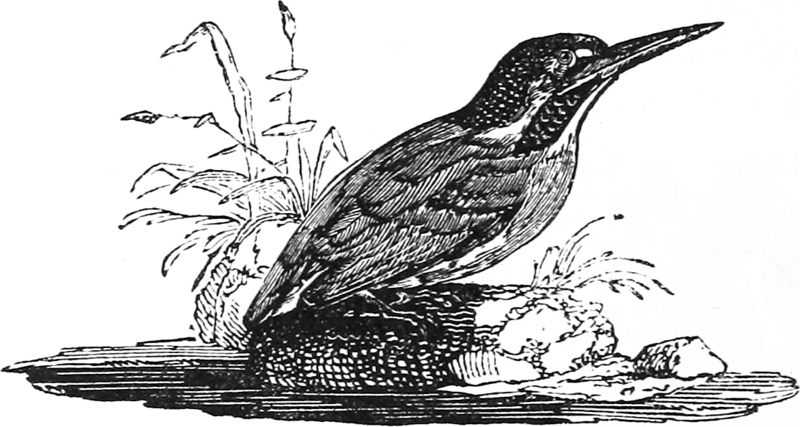
\includegraphics[scale=0.35]{images/Alycon.png}
        \end{figure}
        \vspace{0.5cm}
        \Huge
        \textbf{\textsc{Matematyka Dyskretna}}
        
        \vspace{0.5cm}
        \Large
        \textsc{Wybrane Dowody}
        
        \normalsize
        
        
        \line(1,0){330}
        
        \vspace{1cm}
        \textit{,,Myślę, że 7 punktów na 20 to nie jest zły wynik''}
        \vspace{1cm}

        \textit{\textsc{Popełnione przez}}\\
        \vspace{5mm}

        \textbf{\textsc{Dziurawy Ponton \\ Załatany Ponton \\ Puchaty Pompon \\ Zatopiony Ponton \\ Tonący Ponton \\ Notnop}}

        \vfill

        Kraków \\
        Anno Domini 2023
        
    \end{center}
    
\end{titlepage}


\tableofcontents
\section*{Licencja}
    \begin{figure}[h]
    	\begin{minipage}[c]{0.25\textwidth}
    		
\includegraphics[width=0.7\textwidth]{images/licencja.png}
    	\end{minipage}\hfill
    	\begin{minipage}[c]{0.75\textwidth}
    		\caption*{
    			Ten utwór jest dostępny na 
    			\href{https://creativecommons.org/licenses/by-sa/4.0/}{licencji Creative Commons Uznanie autorstwa
    			na tych samych warunkach 4.0 Międzynarodowe.}
    		}
    	\end{minipage}
    \end{figure}

% Actual content
\mainmatter

\chapter{Kombinatoryka}
 % Żeby nie było syfu to kolejne sekcje dodajemy do chapters/
% A potem includujemy za pomocą \input{chapters/...}

% Używamy \( \) i \[ \] zamiast dolarów -- tak jak się robi w LaTeXu


\documentclass[12pt, a4paper, polish, openany]{book}

% Please, let's familiarize ourselves with notatki.sty and tcs.sty so that we don't reinvent the wheel
\usepackage{notatki}

\fancyhead[L]{\textbf{\textit{MD}}}
\author{
}
\title{TCS and shitposting}


\begin{document}

% Front page and table of contents
\frontmatter

\input{titlepage}

\tableofcontents
\input{license}

% Actual content
\mainmatter

\chapter{Kombinatoryka}
\input{chapters/combinatorics/main}

\chapter{Zasada włączeń i wyłączeń}
\input{chapters/exclusion-inclusion/main}

\chapter{Posety}
\input{chapters/posets/main}

\chapter{Twierdzenie Ramseya}
\input{chapters/ramsey/main}

\chapter{Funkcje tworzące}
\input{chapters/generating_functions/main}

\chapter{Przepływy}
\input{chapters/flows/main}

\chapter{Skojarzenia}
\input{chapters/matchings/main}

\chapter{Kolorowanie grafów}
\input{chapters/graph-coloring/main}

\chapter{Grafy, ale nie kolorowanie}
\input{chapters/graph-misc/main}

\end{document}

\chapter{Zasada włączeń i wyłączeń}
 % Żeby nie było syfu to kolejne sekcje dodajemy do chapters/
% A potem includujemy za pomocą \input{chapters/...}

% Używamy \( \) i \[ \] zamiast dolarów -- tak jak się robi w LaTeXu


\documentclass[12pt, a4paper, polish, openany]{book}

% Please, let's familiarize ourselves with notatki.sty and tcs.sty so that we don't reinvent the wheel
\usepackage{notatki}

\fancyhead[L]{\textbf{\textit{MD}}}
\author{
}
\title{TCS and shitposting}


\begin{document}

% Front page and table of contents
\frontmatter

\input{titlepage}

\tableofcontents
\input{license}

% Actual content
\mainmatter

\chapter{Kombinatoryka}
\input{chapters/combinatorics/main}

\chapter{Zasada włączeń i wyłączeń}
\input{chapters/exclusion-inclusion/main}

\chapter{Posety}
\input{chapters/posets/main}

\chapter{Twierdzenie Ramseya}
\input{chapters/ramsey/main}

\chapter{Funkcje tworzące}
\input{chapters/generating_functions/main}

\chapter{Przepływy}
\input{chapters/flows/main}

\chapter{Skojarzenia}
\input{chapters/matchings/main}

\chapter{Kolorowanie grafów}
\input{chapters/graph-coloring/main}

\chapter{Grafy, ale nie kolorowanie}
\input{chapters/graph-misc/main}

\end{document}

\chapter{Posety}
 % Żeby nie było syfu to kolejne sekcje dodajemy do chapters/
% A potem includujemy za pomocą \input{chapters/...}

% Używamy \( \) i \[ \] zamiast dolarów -- tak jak się robi w LaTeXu


\documentclass[12pt, a4paper, polish, openany]{book}

% Please, let's familiarize ourselves with notatki.sty and tcs.sty so that we don't reinvent the wheel
\usepackage{notatki}

\fancyhead[L]{\textbf{\textit{MD}}}
\author{
}
\title{TCS and shitposting}


\begin{document}

% Front page and table of contents
\frontmatter

\input{titlepage}

\tableofcontents
\input{license}

% Actual content
\mainmatter

\chapter{Kombinatoryka}
\input{chapters/combinatorics/main}

\chapter{Zasada włączeń i wyłączeń}
\input{chapters/exclusion-inclusion/main}

\chapter{Posety}
\input{chapters/posets/main}

\chapter{Twierdzenie Ramseya}
\input{chapters/ramsey/main}

\chapter{Funkcje tworzące}
\input{chapters/generating_functions/main}

\chapter{Przepływy}
\input{chapters/flows/main}

\chapter{Skojarzenia}
\input{chapters/matchings/main}

\chapter{Kolorowanie grafów}
\input{chapters/graph-coloring/main}

\chapter{Grafy, ale nie kolorowanie}
\input{chapters/graph-misc/main}

\end{document}

\chapter{Twierdzenie Ramseya}
 % Żeby nie było syfu to kolejne sekcje dodajemy do chapters/
% A potem includujemy za pomocą \input{chapters/...}

% Używamy \( \) i \[ \] zamiast dolarów -- tak jak się robi w LaTeXu


\documentclass[12pt, a4paper, polish, openany]{book}

% Please, let's familiarize ourselves with notatki.sty and tcs.sty so that we don't reinvent the wheel
\usepackage{notatki}

\fancyhead[L]{\textbf{\textit{MD}}}
\author{
}
\title{TCS and shitposting}


\begin{document}

% Front page and table of contents
\frontmatter

\input{titlepage}

\tableofcontents
\input{license}

% Actual content
\mainmatter

\chapter{Kombinatoryka}
\input{chapters/combinatorics/main}

\chapter{Zasada włączeń i wyłączeń}
\input{chapters/exclusion-inclusion/main}

\chapter{Posety}
\input{chapters/posets/main}

\chapter{Twierdzenie Ramseya}
\input{chapters/ramsey/main}

\chapter{Funkcje tworzące}
\input{chapters/generating_functions/main}

\chapter{Przepływy}
\input{chapters/flows/main}

\chapter{Skojarzenia}
\input{chapters/matchings/main}

\chapter{Kolorowanie grafów}
\input{chapters/graph-coloring/main}

\chapter{Grafy, ale nie kolorowanie}
\input{chapters/graph-misc/main}

\end{document}

\chapter{Funkcje tworzące}
 % Żeby nie było syfu to kolejne sekcje dodajemy do chapters/
% A potem includujemy za pomocą \input{chapters/...}

% Używamy \( \) i \[ \] zamiast dolarów -- tak jak się robi w LaTeXu


\documentclass[12pt, a4paper, polish, openany]{book}

% Please, let's familiarize ourselves with notatki.sty and tcs.sty so that we don't reinvent the wheel
\usepackage{notatki}

\fancyhead[L]{\textbf{\textit{MD}}}
\author{
}
\title{TCS and shitposting}


\begin{document}

% Front page and table of contents
\frontmatter

\input{titlepage}

\tableofcontents
\input{license}

% Actual content
\mainmatter

\chapter{Kombinatoryka}
\input{chapters/combinatorics/main}

\chapter{Zasada włączeń i wyłączeń}
\input{chapters/exclusion-inclusion/main}

\chapter{Posety}
\input{chapters/posets/main}

\chapter{Twierdzenie Ramseya}
\input{chapters/ramsey/main}

\chapter{Funkcje tworzące}
\input{chapters/generating_functions/main}

\chapter{Przepływy}
\input{chapters/flows/main}

\chapter{Skojarzenia}
\input{chapters/matchings/main}

\chapter{Kolorowanie grafów}
\input{chapters/graph-coloring/main}

\chapter{Grafy, ale nie kolorowanie}
\input{chapters/graph-misc/main}

\end{document}

\chapter{Przepływy}
 % Żeby nie było syfu to kolejne sekcje dodajemy do chapters/
% A potem includujemy za pomocą \input{chapters/...}

% Używamy \( \) i \[ \] zamiast dolarów -- tak jak się robi w LaTeXu


\documentclass[12pt, a4paper, polish, openany]{book}

% Please, let's familiarize ourselves with notatki.sty and tcs.sty so that we don't reinvent the wheel
\usepackage{notatki}

\fancyhead[L]{\textbf{\textit{MD}}}
\author{
}
\title{TCS and shitposting}


\begin{document}

% Front page and table of contents
\frontmatter

\input{titlepage}

\tableofcontents
\input{license}

% Actual content
\mainmatter

\chapter{Kombinatoryka}
\input{chapters/combinatorics/main}

\chapter{Zasada włączeń i wyłączeń}
\input{chapters/exclusion-inclusion/main}

\chapter{Posety}
\input{chapters/posets/main}

\chapter{Twierdzenie Ramseya}
\input{chapters/ramsey/main}

\chapter{Funkcje tworzące}
\input{chapters/generating_functions/main}

\chapter{Przepływy}
\input{chapters/flows/main}

\chapter{Skojarzenia}
\input{chapters/matchings/main}

\chapter{Kolorowanie grafów}
\input{chapters/graph-coloring/main}

\chapter{Grafy, ale nie kolorowanie}
\input{chapters/graph-misc/main}

\end{document}

\chapter{Skojarzenia}
 % Żeby nie było syfu to kolejne sekcje dodajemy do chapters/
% A potem includujemy za pomocą \input{chapters/...}

% Używamy \( \) i \[ \] zamiast dolarów -- tak jak się robi w LaTeXu


\documentclass[12pt, a4paper, polish, openany]{book}

% Please, let's familiarize ourselves with notatki.sty and tcs.sty so that we don't reinvent the wheel
\usepackage{notatki}

\fancyhead[L]{\textbf{\textit{MD}}}
\author{
}
\title{TCS and shitposting}


\begin{document}

% Front page and table of contents
\frontmatter

\input{titlepage}

\tableofcontents
\input{license}

% Actual content
\mainmatter

\chapter{Kombinatoryka}
\input{chapters/combinatorics/main}

\chapter{Zasada włączeń i wyłączeń}
\input{chapters/exclusion-inclusion/main}

\chapter{Posety}
\input{chapters/posets/main}

\chapter{Twierdzenie Ramseya}
\input{chapters/ramsey/main}

\chapter{Funkcje tworzące}
\input{chapters/generating_functions/main}

\chapter{Przepływy}
\input{chapters/flows/main}

\chapter{Skojarzenia}
\input{chapters/matchings/main}

\chapter{Kolorowanie grafów}
\input{chapters/graph-coloring/main}

\chapter{Grafy, ale nie kolorowanie}
\input{chapters/graph-misc/main}

\end{document}

\chapter{Kolorowanie grafów}
 % Żeby nie było syfu to kolejne sekcje dodajemy do chapters/
% A potem includujemy za pomocą \input{chapters/...}

% Używamy \( \) i \[ \] zamiast dolarów -- tak jak się robi w LaTeXu


\documentclass[12pt, a4paper, polish, openany]{book}

% Please, let's familiarize ourselves with notatki.sty and tcs.sty so that we don't reinvent the wheel
\usepackage{notatki}

\fancyhead[L]{\textbf{\textit{MD}}}
\author{
}
\title{TCS and shitposting}


\begin{document}

% Front page and table of contents
\frontmatter

\input{titlepage}

\tableofcontents
\input{license}

% Actual content
\mainmatter

\chapter{Kombinatoryka}
\input{chapters/combinatorics/main}

\chapter{Zasada włączeń i wyłączeń}
\input{chapters/exclusion-inclusion/main}

\chapter{Posety}
\input{chapters/posets/main}

\chapter{Twierdzenie Ramseya}
\input{chapters/ramsey/main}

\chapter{Funkcje tworzące}
\input{chapters/generating_functions/main}

\chapter{Przepływy}
\input{chapters/flows/main}

\chapter{Skojarzenia}
\input{chapters/matchings/main}

\chapter{Kolorowanie grafów}
\input{chapters/graph-coloring/main}

\chapter{Grafy, ale nie kolorowanie}
\input{chapters/graph-misc/main}

\end{document}

\chapter{Grafy, ale nie kolorowanie}
 % Żeby nie było syfu to kolejne sekcje dodajemy do chapters/
% A potem includujemy za pomocą \input{chapters/...}

% Używamy \( \) i \[ \] zamiast dolarów -- tak jak się robi w LaTeXu


\documentclass[12pt, a4paper, polish, openany]{book}

% Please, let's familiarize ourselves with notatki.sty and tcs.sty so that we don't reinvent the wheel
\usepackage{notatki}

\fancyhead[L]{\textbf{\textit{MD}}}
\author{
}
\title{TCS and shitposting}


\begin{document}

% Front page and table of contents
\frontmatter

\input{titlepage}

\tableofcontents
\input{license}

% Actual content
\mainmatter

\chapter{Kombinatoryka}
\input{chapters/combinatorics/main}

\chapter{Zasada włączeń i wyłączeń}
\input{chapters/exclusion-inclusion/main}

\chapter{Posety}
\input{chapters/posets/main}

\chapter{Twierdzenie Ramseya}
\input{chapters/ramsey/main}

\chapter{Funkcje tworzące}
\input{chapters/generating_functions/main}

\chapter{Przepływy}
\input{chapters/flows/main}

\chapter{Skojarzenia}
\input{chapters/matchings/main}

\chapter{Kolorowanie grafów}
\input{chapters/graph-coloring/main}

\chapter{Grafy, ale nie kolorowanie}
\input{chapters/graph-misc/main}

\end{document}

\end{document}

\chapter{Posety}
 % Żeby nie było syfu to kolejne sekcje dodajemy do chapters/
% A potem includujemy za pomocą \input{chapters/...}

% Używamy \( \) i \[ \] zamiast dolarów -- tak jak się robi w LaTeXu


\documentclass[12pt, a4paper, polish, openany]{book}

% Please, let's familiarize ourselves with notatki.sty and tcs.sty so that we don't reinvent the wheel
\usepackage{notatki}

\fancyhead[L]{\textbf{\textit{MD}}}
\author{
}
\title{TCS and shitposting}


\begin{document}

% Front page and table of contents
\frontmatter

\begin{titlepage} 

    \begin{center}
         \begin{figure}[h]
            \centering
            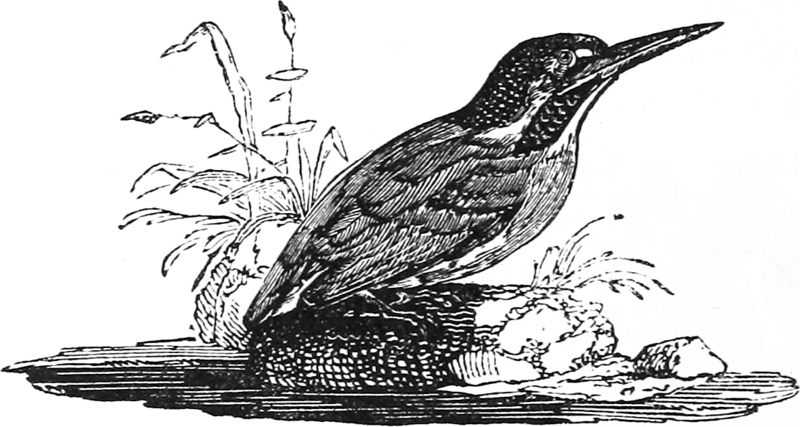
\includegraphics[scale=0.35]{images/Alycon.png}
        \end{figure}
        \vspace{0.5cm}
        \Huge
        \textbf{\textsc{Matematyka Dyskretna}}
        
        \vspace{0.5cm}
        \Large
        \textsc{Wybrane Dowody}
        
        \normalsize
        
        
        \line(1,0){330}
        
        \vspace{1cm}
        \textit{,,Myślę, że 7 punktów na 20 to nie jest zły wynik''}
        \vspace{1cm}

        \textit{\textsc{Popełnione przez}}\\
        \vspace{5mm}

        \textbf{\textsc{Dziurawy Ponton \\ Załatany Ponton \\ Puchaty Pompon \\ Zatopiony Ponton \\ Tonący Ponton \\ Notnop}}

        \vfill

        Kraków \\
        Anno Domini 2023
        
    \end{center}
    
\end{titlepage}


\tableofcontents
\section*{Licencja}
    \begin{figure}[h]
    	\begin{minipage}[c]{0.25\textwidth}
    		
\includegraphics[width=0.7\textwidth]{images/licencja.png}
    	\end{minipage}\hfill
    	\begin{minipage}[c]{0.75\textwidth}
    		\caption*{
    			Ten utwór jest dostępny na 
    			\href{https://creativecommons.org/licenses/by-sa/4.0/}{licencji Creative Commons Uznanie autorstwa
    			na tych samych warunkach 4.0 Międzynarodowe.}
    		}
    	\end{minipage}
    \end{figure}

% Actual content
\mainmatter

\chapter{Kombinatoryka}
 % Żeby nie było syfu to kolejne sekcje dodajemy do chapters/
% A potem includujemy za pomocą \input{chapters/...}

% Używamy \( \) i \[ \] zamiast dolarów -- tak jak się robi w LaTeXu


\documentclass[12pt, a4paper, polish, openany]{book}

% Please, let's familiarize ourselves with notatki.sty and tcs.sty so that we don't reinvent the wheel
\usepackage{notatki}

\fancyhead[L]{\textbf{\textit{MD}}}
\author{
}
\title{TCS and shitposting}


\begin{document}

% Front page and table of contents
\frontmatter

\input{titlepage}

\tableofcontents
\input{license}

% Actual content
\mainmatter

\chapter{Kombinatoryka}
\input{chapters/combinatorics/main}

\chapter{Zasada włączeń i wyłączeń}
\input{chapters/exclusion-inclusion/main}

\chapter{Posety}
\input{chapters/posets/main}

\chapter{Twierdzenie Ramseya}
\input{chapters/ramsey/main}

\chapter{Funkcje tworzące}
\input{chapters/generating_functions/main}

\chapter{Przepływy}
\input{chapters/flows/main}

\chapter{Skojarzenia}
\input{chapters/matchings/main}

\chapter{Kolorowanie grafów}
\input{chapters/graph-coloring/main}

\chapter{Grafy, ale nie kolorowanie}
\input{chapters/graph-misc/main}

\end{document}

\chapter{Zasada włączeń i wyłączeń}
 % Żeby nie było syfu to kolejne sekcje dodajemy do chapters/
% A potem includujemy za pomocą \input{chapters/...}

% Używamy \( \) i \[ \] zamiast dolarów -- tak jak się robi w LaTeXu


\documentclass[12pt, a4paper, polish, openany]{book}

% Please, let's familiarize ourselves with notatki.sty and tcs.sty so that we don't reinvent the wheel
\usepackage{notatki}

\fancyhead[L]{\textbf{\textit{MD}}}
\author{
}
\title{TCS and shitposting}


\begin{document}

% Front page and table of contents
\frontmatter

\input{titlepage}

\tableofcontents
\input{license}

% Actual content
\mainmatter

\chapter{Kombinatoryka}
\input{chapters/combinatorics/main}

\chapter{Zasada włączeń i wyłączeń}
\input{chapters/exclusion-inclusion/main}

\chapter{Posety}
\input{chapters/posets/main}

\chapter{Twierdzenie Ramseya}
\input{chapters/ramsey/main}

\chapter{Funkcje tworzące}
\input{chapters/generating_functions/main}

\chapter{Przepływy}
\input{chapters/flows/main}

\chapter{Skojarzenia}
\input{chapters/matchings/main}

\chapter{Kolorowanie grafów}
\input{chapters/graph-coloring/main}

\chapter{Grafy, ale nie kolorowanie}
\input{chapters/graph-misc/main}

\end{document}

\chapter{Posety}
 % Żeby nie było syfu to kolejne sekcje dodajemy do chapters/
% A potem includujemy za pomocą \input{chapters/...}

% Używamy \( \) i \[ \] zamiast dolarów -- tak jak się robi w LaTeXu


\documentclass[12pt, a4paper, polish, openany]{book}

% Please, let's familiarize ourselves with notatki.sty and tcs.sty so that we don't reinvent the wheel
\usepackage{notatki}

\fancyhead[L]{\textbf{\textit{MD}}}
\author{
}
\title{TCS and shitposting}


\begin{document}

% Front page and table of contents
\frontmatter

\input{titlepage}

\tableofcontents
\input{license}

% Actual content
\mainmatter

\chapter{Kombinatoryka}
\input{chapters/combinatorics/main}

\chapter{Zasada włączeń i wyłączeń}
\input{chapters/exclusion-inclusion/main}

\chapter{Posety}
\input{chapters/posets/main}

\chapter{Twierdzenie Ramseya}
\input{chapters/ramsey/main}

\chapter{Funkcje tworzące}
\input{chapters/generating_functions/main}

\chapter{Przepływy}
\input{chapters/flows/main}

\chapter{Skojarzenia}
\input{chapters/matchings/main}

\chapter{Kolorowanie grafów}
\input{chapters/graph-coloring/main}

\chapter{Grafy, ale nie kolorowanie}
\input{chapters/graph-misc/main}

\end{document}

\chapter{Twierdzenie Ramseya}
 % Żeby nie było syfu to kolejne sekcje dodajemy do chapters/
% A potem includujemy za pomocą \input{chapters/...}

% Używamy \( \) i \[ \] zamiast dolarów -- tak jak się robi w LaTeXu


\documentclass[12pt, a4paper, polish, openany]{book}

% Please, let's familiarize ourselves with notatki.sty and tcs.sty so that we don't reinvent the wheel
\usepackage{notatki}

\fancyhead[L]{\textbf{\textit{MD}}}
\author{
}
\title{TCS and shitposting}


\begin{document}

% Front page and table of contents
\frontmatter

\input{titlepage}

\tableofcontents
\input{license}

% Actual content
\mainmatter

\chapter{Kombinatoryka}
\input{chapters/combinatorics/main}

\chapter{Zasada włączeń i wyłączeń}
\input{chapters/exclusion-inclusion/main}

\chapter{Posety}
\input{chapters/posets/main}

\chapter{Twierdzenie Ramseya}
\input{chapters/ramsey/main}

\chapter{Funkcje tworzące}
\input{chapters/generating_functions/main}

\chapter{Przepływy}
\input{chapters/flows/main}

\chapter{Skojarzenia}
\input{chapters/matchings/main}

\chapter{Kolorowanie grafów}
\input{chapters/graph-coloring/main}

\chapter{Grafy, ale nie kolorowanie}
\input{chapters/graph-misc/main}

\end{document}

\chapter{Funkcje tworzące}
 % Żeby nie było syfu to kolejne sekcje dodajemy do chapters/
% A potem includujemy za pomocą \input{chapters/...}

% Używamy \( \) i \[ \] zamiast dolarów -- tak jak się robi w LaTeXu


\documentclass[12pt, a4paper, polish, openany]{book}

% Please, let's familiarize ourselves with notatki.sty and tcs.sty so that we don't reinvent the wheel
\usepackage{notatki}

\fancyhead[L]{\textbf{\textit{MD}}}
\author{
}
\title{TCS and shitposting}


\begin{document}

% Front page and table of contents
\frontmatter

\input{titlepage}

\tableofcontents
\input{license}

% Actual content
\mainmatter

\chapter{Kombinatoryka}
\input{chapters/combinatorics/main}

\chapter{Zasada włączeń i wyłączeń}
\input{chapters/exclusion-inclusion/main}

\chapter{Posety}
\input{chapters/posets/main}

\chapter{Twierdzenie Ramseya}
\input{chapters/ramsey/main}

\chapter{Funkcje tworzące}
\input{chapters/generating_functions/main}

\chapter{Przepływy}
\input{chapters/flows/main}

\chapter{Skojarzenia}
\input{chapters/matchings/main}

\chapter{Kolorowanie grafów}
\input{chapters/graph-coloring/main}

\chapter{Grafy, ale nie kolorowanie}
\input{chapters/graph-misc/main}

\end{document}

\chapter{Przepływy}
 % Żeby nie było syfu to kolejne sekcje dodajemy do chapters/
% A potem includujemy za pomocą \input{chapters/...}

% Używamy \( \) i \[ \] zamiast dolarów -- tak jak się robi w LaTeXu


\documentclass[12pt, a4paper, polish, openany]{book}

% Please, let's familiarize ourselves with notatki.sty and tcs.sty so that we don't reinvent the wheel
\usepackage{notatki}

\fancyhead[L]{\textbf{\textit{MD}}}
\author{
}
\title{TCS and shitposting}


\begin{document}

% Front page and table of contents
\frontmatter

\input{titlepage}

\tableofcontents
\input{license}

% Actual content
\mainmatter

\chapter{Kombinatoryka}
\input{chapters/combinatorics/main}

\chapter{Zasada włączeń i wyłączeń}
\input{chapters/exclusion-inclusion/main}

\chapter{Posety}
\input{chapters/posets/main}

\chapter{Twierdzenie Ramseya}
\input{chapters/ramsey/main}

\chapter{Funkcje tworzące}
\input{chapters/generating_functions/main}

\chapter{Przepływy}
\input{chapters/flows/main}

\chapter{Skojarzenia}
\input{chapters/matchings/main}

\chapter{Kolorowanie grafów}
\input{chapters/graph-coloring/main}

\chapter{Grafy, ale nie kolorowanie}
\input{chapters/graph-misc/main}

\end{document}

\chapter{Skojarzenia}
 % Żeby nie było syfu to kolejne sekcje dodajemy do chapters/
% A potem includujemy za pomocą \input{chapters/...}

% Używamy \( \) i \[ \] zamiast dolarów -- tak jak się robi w LaTeXu


\documentclass[12pt, a4paper, polish, openany]{book}

% Please, let's familiarize ourselves with notatki.sty and tcs.sty so that we don't reinvent the wheel
\usepackage{notatki}

\fancyhead[L]{\textbf{\textit{MD}}}
\author{
}
\title{TCS and shitposting}


\begin{document}

% Front page and table of contents
\frontmatter

\input{titlepage}

\tableofcontents
\input{license}

% Actual content
\mainmatter

\chapter{Kombinatoryka}
\input{chapters/combinatorics/main}

\chapter{Zasada włączeń i wyłączeń}
\input{chapters/exclusion-inclusion/main}

\chapter{Posety}
\input{chapters/posets/main}

\chapter{Twierdzenie Ramseya}
\input{chapters/ramsey/main}

\chapter{Funkcje tworzące}
\input{chapters/generating_functions/main}

\chapter{Przepływy}
\input{chapters/flows/main}

\chapter{Skojarzenia}
\input{chapters/matchings/main}

\chapter{Kolorowanie grafów}
\input{chapters/graph-coloring/main}

\chapter{Grafy, ale nie kolorowanie}
\input{chapters/graph-misc/main}

\end{document}

\chapter{Kolorowanie grafów}
 % Żeby nie było syfu to kolejne sekcje dodajemy do chapters/
% A potem includujemy za pomocą \input{chapters/...}

% Używamy \( \) i \[ \] zamiast dolarów -- tak jak się robi w LaTeXu


\documentclass[12pt, a4paper, polish, openany]{book}

% Please, let's familiarize ourselves with notatki.sty and tcs.sty so that we don't reinvent the wheel
\usepackage{notatki}

\fancyhead[L]{\textbf{\textit{MD}}}
\author{
}
\title{TCS and shitposting}


\begin{document}

% Front page and table of contents
\frontmatter

\input{titlepage}

\tableofcontents
\input{license}

% Actual content
\mainmatter

\chapter{Kombinatoryka}
\input{chapters/combinatorics/main}

\chapter{Zasada włączeń i wyłączeń}
\input{chapters/exclusion-inclusion/main}

\chapter{Posety}
\input{chapters/posets/main}

\chapter{Twierdzenie Ramseya}
\input{chapters/ramsey/main}

\chapter{Funkcje tworzące}
\input{chapters/generating_functions/main}

\chapter{Przepływy}
\input{chapters/flows/main}

\chapter{Skojarzenia}
\input{chapters/matchings/main}

\chapter{Kolorowanie grafów}
\input{chapters/graph-coloring/main}

\chapter{Grafy, ale nie kolorowanie}
\input{chapters/graph-misc/main}

\end{document}

\chapter{Grafy, ale nie kolorowanie}
 % Żeby nie było syfu to kolejne sekcje dodajemy do chapters/
% A potem includujemy za pomocą \input{chapters/...}

% Używamy \( \) i \[ \] zamiast dolarów -- tak jak się robi w LaTeXu


\documentclass[12pt, a4paper, polish, openany]{book}

% Please, let's familiarize ourselves with notatki.sty and tcs.sty so that we don't reinvent the wheel
\usepackage{notatki}

\fancyhead[L]{\textbf{\textit{MD}}}
\author{
}
\title{TCS and shitposting}


\begin{document}

% Front page and table of contents
\frontmatter

\input{titlepage}

\tableofcontents
\input{license}

% Actual content
\mainmatter

\chapter{Kombinatoryka}
\input{chapters/combinatorics/main}

\chapter{Zasada włączeń i wyłączeń}
\input{chapters/exclusion-inclusion/main}

\chapter{Posety}
\input{chapters/posets/main}

\chapter{Twierdzenie Ramseya}
\input{chapters/ramsey/main}

\chapter{Funkcje tworzące}
\input{chapters/generating_functions/main}

\chapter{Przepływy}
\input{chapters/flows/main}

\chapter{Skojarzenia}
\input{chapters/matchings/main}

\chapter{Kolorowanie grafów}
\input{chapters/graph-coloring/main}

\chapter{Grafy, ale nie kolorowanie}
\input{chapters/graph-misc/main}

\end{document}

\end{document}

\chapter{Twierdzenie Ramseya}
 % Żeby nie było syfu to kolejne sekcje dodajemy do chapters/
% A potem includujemy za pomocą \input{chapters/...}

% Używamy \( \) i \[ \] zamiast dolarów -- tak jak się robi w LaTeXu


\documentclass[12pt, a4paper, polish, openany]{book}

% Please, let's familiarize ourselves with notatki.sty and tcs.sty so that we don't reinvent the wheel
\usepackage{notatki}

\fancyhead[L]{\textbf{\textit{MD}}}
\author{
}
\title{TCS and shitposting}


\begin{document}

% Front page and table of contents
\frontmatter

\begin{titlepage} 

    \begin{center}
         \begin{figure}[h]
            \centering
            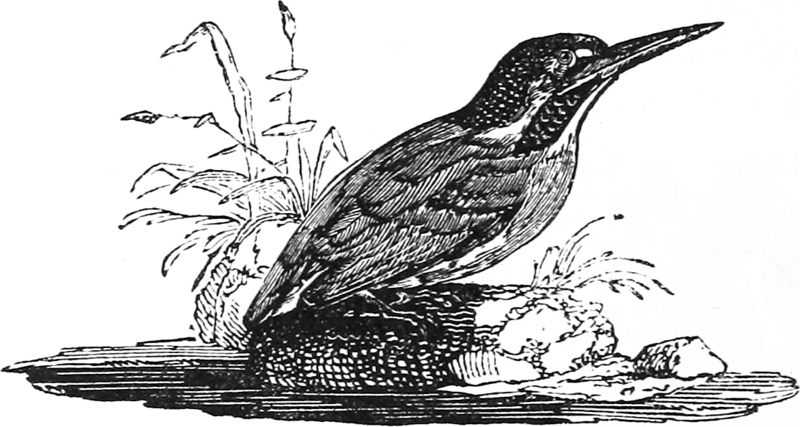
\includegraphics[scale=0.35]{images/Alycon.png}
        \end{figure}
        \vspace{0.5cm}
        \Huge
        \textbf{\textsc{Matematyka Dyskretna}}
        
        \vspace{0.5cm}
        \Large
        \textsc{Wybrane Dowody}
        
        \normalsize
        
        
        \line(1,0){330}
        
        \vspace{1cm}
        \textit{,,Myślę, że 7 punktów na 20 to nie jest zły wynik''}
        \vspace{1cm}

        \textit{\textsc{Popełnione przez}}\\
        \vspace{5mm}

        \textbf{\textsc{Dziurawy Ponton \\ Załatany Ponton \\ Puchaty Pompon \\ Zatopiony Ponton \\ Tonący Ponton \\ Notnop}}

        \vfill

        Kraków \\
        Anno Domini 2023
        
    \end{center}
    
\end{titlepage}


\tableofcontents
\section*{Licencja}
    \begin{figure}[h]
    	\begin{minipage}[c]{0.25\textwidth}
    		
\includegraphics[width=0.7\textwidth]{images/licencja.png}
    	\end{minipage}\hfill
    	\begin{minipage}[c]{0.75\textwidth}
    		\caption*{
    			Ten utwór jest dostępny na 
    			\href{https://creativecommons.org/licenses/by-sa/4.0/}{licencji Creative Commons Uznanie autorstwa
    			na tych samych warunkach 4.0 Międzynarodowe.}
    		}
    	\end{minipage}
    \end{figure}

% Actual content
\mainmatter

\chapter{Kombinatoryka}
 % Żeby nie było syfu to kolejne sekcje dodajemy do chapters/
% A potem includujemy za pomocą \input{chapters/...}

% Używamy \( \) i \[ \] zamiast dolarów -- tak jak się robi w LaTeXu


\documentclass[12pt, a4paper, polish, openany]{book}

% Please, let's familiarize ourselves with notatki.sty and tcs.sty so that we don't reinvent the wheel
\usepackage{notatki}

\fancyhead[L]{\textbf{\textit{MD}}}
\author{
}
\title{TCS and shitposting}


\begin{document}

% Front page and table of contents
\frontmatter

\input{titlepage}

\tableofcontents
\input{license}

% Actual content
\mainmatter

\chapter{Kombinatoryka}
\input{chapters/combinatorics/main}

\chapter{Zasada włączeń i wyłączeń}
\input{chapters/exclusion-inclusion/main}

\chapter{Posety}
\input{chapters/posets/main}

\chapter{Twierdzenie Ramseya}
\input{chapters/ramsey/main}

\chapter{Funkcje tworzące}
\input{chapters/generating_functions/main}

\chapter{Przepływy}
\input{chapters/flows/main}

\chapter{Skojarzenia}
\input{chapters/matchings/main}

\chapter{Kolorowanie grafów}
\input{chapters/graph-coloring/main}

\chapter{Grafy, ale nie kolorowanie}
\input{chapters/graph-misc/main}

\end{document}

\chapter{Zasada włączeń i wyłączeń}
 % Żeby nie było syfu to kolejne sekcje dodajemy do chapters/
% A potem includujemy za pomocą \input{chapters/...}

% Używamy \( \) i \[ \] zamiast dolarów -- tak jak się robi w LaTeXu


\documentclass[12pt, a4paper, polish, openany]{book}

% Please, let's familiarize ourselves with notatki.sty and tcs.sty so that we don't reinvent the wheel
\usepackage{notatki}

\fancyhead[L]{\textbf{\textit{MD}}}
\author{
}
\title{TCS and shitposting}


\begin{document}

% Front page and table of contents
\frontmatter

\input{titlepage}

\tableofcontents
\input{license}

% Actual content
\mainmatter

\chapter{Kombinatoryka}
\input{chapters/combinatorics/main}

\chapter{Zasada włączeń i wyłączeń}
\input{chapters/exclusion-inclusion/main}

\chapter{Posety}
\input{chapters/posets/main}

\chapter{Twierdzenie Ramseya}
\input{chapters/ramsey/main}

\chapter{Funkcje tworzące}
\input{chapters/generating_functions/main}

\chapter{Przepływy}
\input{chapters/flows/main}

\chapter{Skojarzenia}
\input{chapters/matchings/main}

\chapter{Kolorowanie grafów}
\input{chapters/graph-coloring/main}

\chapter{Grafy, ale nie kolorowanie}
\input{chapters/graph-misc/main}

\end{document}

\chapter{Posety}
 % Żeby nie było syfu to kolejne sekcje dodajemy do chapters/
% A potem includujemy za pomocą \input{chapters/...}

% Używamy \( \) i \[ \] zamiast dolarów -- tak jak się robi w LaTeXu


\documentclass[12pt, a4paper, polish, openany]{book}

% Please, let's familiarize ourselves with notatki.sty and tcs.sty so that we don't reinvent the wheel
\usepackage{notatki}

\fancyhead[L]{\textbf{\textit{MD}}}
\author{
}
\title{TCS and shitposting}


\begin{document}

% Front page and table of contents
\frontmatter

\input{titlepage}

\tableofcontents
\input{license}

% Actual content
\mainmatter

\chapter{Kombinatoryka}
\input{chapters/combinatorics/main}

\chapter{Zasada włączeń i wyłączeń}
\input{chapters/exclusion-inclusion/main}

\chapter{Posety}
\input{chapters/posets/main}

\chapter{Twierdzenie Ramseya}
\input{chapters/ramsey/main}

\chapter{Funkcje tworzące}
\input{chapters/generating_functions/main}

\chapter{Przepływy}
\input{chapters/flows/main}

\chapter{Skojarzenia}
\input{chapters/matchings/main}

\chapter{Kolorowanie grafów}
\input{chapters/graph-coloring/main}

\chapter{Grafy, ale nie kolorowanie}
\input{chapters/graph-misc/main}

\end{document}

\chapter{Twierdzenie Ramseya}
 % Żeby nie było syfu to kolejne sekcje dodajemy do chapters/
% A potem includujemy za pomocą \input{chapters/...}

% Używamy \( \) i \[ \] zamiast dolarów -- tak jak się robi w LaTeXu


\documentclass[12pt, a4paper, polish, openany]{book}

% Please, let's familiarize ourselves with notatki.sty and tcs.sty so that we don't reinvent the wheel
\usepackage{notatki}

\fancyhead[L]{\textbf{\textit{MD}}}
\author{
}
\title{TCS and shitposting}


\begin{document}

% Front page and table of contents
\frontmatter

\input{titlepage}

\tableofcontents
\input{license}

% Actual content
\mainmatter

\chapter{Kombinatoryka}
\input{chapters/combinatorics/main}

\chapter{Zasada włączeń i wyłączeń}
\input{chapters/exclusion-inclusion/main}

\chapter{Posety}
\input{chapters/posets/main}

\chapter{Twierdzenie Ramseya}
\input{chapters/ramsey/main}

\chapter{Funkcje tworzące}
\input{chapters/generating_functions/main}

\chapter{Przepływy}
\input{chapters/flows/main}

\chapter{Skojarzenia}
\input{chapters/matchings/main}

\chapter{Kolorowanie grafów}
\input{chapters/graph-coloring/main}

\chapter{Grafy, ale nie kolorowanie}
\input{chapters/graph-misc/main}

\end{document}

\chapter{Funkcje tworzące}
 % Żeby nie było syfu to kolejne sekcje dodajemy do chapters/
% A potem includujemy za pomocą \input{chapters/...}

% Używamy \( \) i \[ \] zamiast dolarów -- tak jak się robi w LaTeXu


\documentclass[12pt, a4paper, polish, openany]{book}

% Please, let's familiarize ourselves with notatki.sty and tcs.sty so that we don't reinvent the wheel
\usepackage{notatki}

\fancyhead[L]{\textbf{\textit{MD}}}
\author{
}
\title{TCS and shitposting}


\begin{document}

% Front page and table of contents
\frontmatter

\input{titlepage}

\tableofcontents
\input{license}

% Actual content
\mainmatter

\chapter{Kombinatoryka}
\input{chapters/combinatorics/main}

\chapter{Zasada włączeń i wyłączeń}
\input{chapters/exclusion-inclusion/main}

\chapter{Posety}
\input{chapters/posets/main}

\chapter{Twierdzenie Ramseya}
\input{chapters/ramsey/main}

\chapter{Funkcje tworzące}
\input{chapters/generating_functions/main}

\chapter{Przepływy}
\input{chapters/flows/main}

\chapter{Skojarzenia}
\input{chapters/matchings/main}

\chapter{Kolorowanie grafów}
\input{chapters/graph-coloring/main}

\chapter{Grafy, ale nie kolorowanie}
\input{chapters/graph-misc/main}

\end{document}

\chapter{Przepływy}
 % Żeby nie było syfu to kolejne sekcje dodajemy do chapters/
% A potem includujemy za pomocą \input{chapters/...}

% Używamy \( \) i \[ \] zamiast dolarów -- tak jak się robi w LaTeXu


\documentclass[12pt, a4paper, polish, openany]{book}

% Please, let's familiarize ourselves with notatki.sty and tcs.sty so that we don't reinvent the wheel
\usepackage{notatki}

\fancyhead[L]{\textbf{\textit{MD}}}
\author{
}
\title{TCS and shitposting}


\begin{document}

% Front page and table of contents
\frontmatter

\input{titlepage}

\tableofcontents
\input{license}

% Actual content
\mainmatter

\chapter{Kombinatoryka}
\input{chapters/combinatorics/main}

\chapter{Zasada włączeń i wyłączeń}
\input{chapters/exclusion-inclusion/main}

\chapter{Posety}
\input{chapters/posets/main}

\chapter{Twierdzenie Ramseya}
\input{chapters/ramsey/main}

\chapter{Funkcje tworzące}
\input{chapters/generating_functions/main}

\chapter{Przepływy}
\input{chapters/flows/main}

\chapter{Skojarzenia}
\input{chapters/matchings/main}

\chapter{Kolorowanie grafów}
\input{chapters/graph-coloring/main}

\chapter{Grafy, ale nie kolorowanie}
\input{chapters/graph-misc/main}

\end{document}

\chapter{Skojarzenia}
 % Żeby nie było syfu to kolejne sekcje dodajemy do chapters/
% A potem includujemy za pomocą \input{chapters/...}

% Używamy \( \) i \[ \] zamiast dolarów -- tak jak się robi w LaTeXu


\documentclass[12pt, a4paper, polish, openany]{book}

% Please, let's familiarize ourselves with notatki.sty and tcs.sty so that we don't reinvent the wheel
\usepackage{notatki}

\fancyhead[L]{\textbf{\textit{MD}}}
\author{
}
\title{TCS and shitposting}


\begin{document}

% Front page and table of contents
\frontmatter

\input{titlepage}

\tableofcontents
\input{license}

% Actual content
\mainmatter

\chapter{Kombinatoryka}
\input{chapters/combinatorics/main}

\chapter{Zasada włączeń i wyłączeń}
\input{chapters/exclusion-inclusion/main}

\chapter{Posety}
\input{chapters/posets/main}

\chapter{Twierdzenie Ramseya}
\input{chapters/ramsey/main}

\chapter{Funkcje tworzące}
\input{chapters/generating_functions/main}

\chapter{Przepływy}
\input{chapters/flows/main}

\chapter{Skojarzenia}
\input{chapters/matchings/main}

\chapter{Kolorowanie grafów}
\input{chapters/graph-coloring/main}

\chapter{Grafy, ale nie kolorowanie}
\input{chapters/graph-misc/main}

\end{document}

\chapter{Kolorowanie grafów}
 % Żeby nie było syfu to kolejne sekcje dodajemy do chapters/
% A potem includujemy za pomocą \input{chapters/...}

% Używamy \( \) i \[ \] zamiast dolarów -- tak jak się robi w LaTeXu


\documentclass[12pt, a4paper, polish, openany]{book}

% Please, let's familiarize ourselves with notatki.sty and tcs.sty so that we don't reinvent the wheel
\usepackage{notatki}

\fancyhead[L]{\textbf{\textit{MD}}}
\author{
}
\title{TCS and shitposting}


\begin{document}

% Front page and table of contents
\frontmatter

\input{titlepage}

\tableofcontents
\input{license}

% Actual content
\mainmatter

\chapter{Kombinatoryka}
\input{chapters/combinatorics/main}

\chapter{Zasada włączeń i wyłączeń}
\input{chapters/exclusion-inclusion/main}

\chapter{Posety}
\input{chapters/posets/main}

\chapter{Twierdzenie Ramseya}
\input{chapters/ramsey/main}

\chapter{Funkcje tworzące}
\input{chapters/generating_functions/main}

\chapter{Przepływy}
\input{chapters/flows/main}

\chapter{Skojarzenia}
\input{chapters/matchings/main}

\chapter{Kolorowanie grafów}
\input{chapters/graph-coloring/main}

\chapter{Grafy, ale nie kolorowanie}
\input{chapters/graph-misc/main}

\end{document}

\chapter{Grafy, ale nie kolorowanie}
 % Żeby nie było syfu to kolejne sekcje dodajemy do chapters/
% A potem includujemy za pomocą \input{chapters/...}

% Używamy \( \) i \[ \] zamiast dolarów -- tak jak się robi w LaTeXu


\documentclass[12pt, a4paper, polish, openany]{book}

% Please, let's familiarize ourselves with notatki.sty and tcs.sty so that we don't reinvent the wheel
\usepackage{notatki}

\fancyhead[L]{\textbf{\textit{MD}}}
\author{
}
\title{TCS and shitposting}


\begin{document}

% Front page and table of contents
\frontmatter

\input{titlepage}

\tableofcontents
\input{license}

% Actual content
\mainmatter

\chapter{Kombinatoryka}
\input{chapters/combinatorics/main}

\chapter{Zasada włączeń i wyłączeń}
\input{chapters/exclusion-inclusion/main}

\chapter{Posety}
\input{chapters/posets/main}

\chapter{Twierdzenie Ramseya}
\input{chapters/ramsey/main}

\chapter{Funkcje tworzące}
\input{chapters/generating_functions/main}

\chapter{Przepływy}
\input{chapters/flows/main}

\chapter{Skojarzenia}
\input{chapters/matchings/main}

\chapter{Kolorowanie grafów}
\input{chapters/graph-coloring/main}

\chapter{Grafy, ale nie kolorowanie}
\input{chapters/graph-misc/main}

\end{document}

\end{document}

\chapter{Funkcje tworzące}
 % Żeby nie było syfu to kolejne sekcje dodajemy do chapters/
% A potem includujemy za pomocą \input{chapters/...}

% Używamy \( \) i \[ \] zamiast dolarów -- tak jak się robi w LaTeXu


\documentclass[12pt, a4paper, polish, openany]{book}

% Please, let's familiarize ourselves with notatki.sty and tcs.sty so that we don't reinvent the wheel
\usepackage{notatki}

\fancyhead[L]{\textbf{\textit{MD}}}
\author{
}
\title{TCS and shitposting}


\begin{document}

% Front page and table of contents
\frontmatter

\begin{titlepage} 

    \begin{center}
         \begin{figure}[h]
            \centering
            \includegraphics[scale=0.35]{images/Alycon.png}
        \end{figure}
        \vspace{0.5cm}
        \Huge
        \textbf{\textsc{Matematyka Dyskretna}}
        
        \vspace{0.5cm}
        \Large
        \textsc{Wybrane Dowody}
        
        \normalsize
        
        
        \line(1,0){330}
        
        \vspace{1cm}
        \textit{,,Myślę, że 7 punktów na 20 to nie jest zły wynik''}
        \vspace{1cm}

        \textit{\textsc{Popełnione przez}}\\
        \vspace{5mm}

        \textbf{\textsc{Dziurawy Ponton \\ Załatany Ponton \\ Puchaty Pompon \\ Zatopiony Ponton \\ Tonący Ponton \\ Notnop}}

        \vfill

        Kraków \\
        Anno Domini 2023
        
    \end{center}
    
\end{titlepage}


\tableofcontents
\section*{Licencja}
    \begin{figure}[h]
    	\begin{minipage}[c]{0.25\textwidth}
    		\includegraphics[width=0.7\textwidth]{images/licencja.png}
    	\end{minipage}\hfill
    	\begin{minipage}[c]{0.75\textwidth}
    		\caption*{
    			Ten utwór jest dostępny na 
    			\href{https://creativecommons.org/licenses/by-sa/4.0/}{licencji Creative Commons Uznanie autorstwa
    			na tych samych warunkach 4.0 Międzynarodowe.}
    		}
    	\end{minipage}
    \end{figure}

% Actual content
\mainmatter

\chapter{Kombinatoryka}
 % Żeby nie było syfu to kolejne sekcje dodajemy do chapters/
% A potem includujemy za pomocą \input{chapters/...}

% Używamy \( \) i \[ \] zamiast dolarów -- tak jak się robi w LaTeXu


\documentclass[12pt, a4paper, polish, openany]{book}

% Please, let's familiarize ourselves with notatki.sty and tcs.sty so that we don't reinvent the wheel
\usepackage{notatki}

\fancyhead[L]{\textbf{\textit{MD}}}
\author{
}
\title{TCS and shitposting}


\begin{document}

% Front page and table of contents
\frontmatter

\input{titlepage}

\tableofcontents
\input{license}

% Actual content
\mainmatter

\chapter{Kombinatoryka}
\input{chapters/combinatorics/main}

\chapter{Zasada włączeń i wyłączeń}
\input{chapters/exclusion-inclusion/main}

\chapter{Posety}
\input{chapters/posets/main}

\chapter{Twierdzenie Ramseya}
\input{chapters/ramsey/main}

\chapter{Funkcje tworzące}
\input{chapters/generating_functions/main}

\chapter{Przepływy}
\input{chapters/flows/main}

\chapter{Skojarzenia}
\input{chapters/matchings/main}

\chapter{Kolorowanie grafów}
\input{chapters/graph-coloring/main}

\chapter{Grafy, ale nie kolorowanie}
\input{chapters/graph-misc/main}

\end{document}

\chapter{Zasada włączeń i wyłączeń}
 % Żeby nie było syfu to kolejne sekcje dodajemy do chapters/
% A potem includujemy za pomocą \input{chapters/...}

% Używamy \( \) i \[ \] zamiast dolarów -- tak jak się robi w LaTeXu


\documentclass[12pt, a4paper, polish, openany]{book}

% Please, let's familiarize ourselves with notatki.sty and tcs.sty so that we don't reinvent the wheel
\usepackage{notatki}

\fancyhead[L]{\textbf{\textit{MD}}}
\author{
}
\title{TCS and shitposting}


\begin{document}

% Front page and table of contents
\frontmatter

\input{titlepage}

\tableofcontents
\input{license}

% Actual content
\mainmatter

\chapter{Kombinatoryka}
\input{chapters/combinatorics/main}

\chapter{Zasada włączeń i wyłączeń}
\input{chapters/exclusion-inclusion/main}

\chapter{Posety}
\input{chapters/posets/main}

\chapter{Twierdzenie Ramseya}
\input{chapters/ramsey/main}

\chapter{Funkcje tworzące}
\input{chapters/generating_functions/main}

\chapter{Przepływy}
\input{chapters/flows/main}

\chapter{Skojarzenia}
\input{chapters/matchings/main}

\chapter{Kolorowanie grafów}
\input{chapters/graph-coloring/main}

\chapter{Grafy, ale nie kolorowanie}
\input{chapters/graph-misc/main}

\end{document}

\chapter{Posety}
 % Żeby nie było syfu to kolejne sekcje dodajemy do chapters/
% A potem includujemy za pomocą \input{chapters/...}

% Używamy \( \) i \[ \] zamiast dolarów -- tak jak się robi w LaTeXu


\documentclass[12pt, a4paper, polish, openany]{book}

% Please, let's familiarize ourselves with notatki.sty and tcs.sty so that we don't reinvent the wheel
\usepackage{notatki}

\fancyhead[L]{\textbf{\textit{MD}}}
\author{
}
\title{TCS and shitposting}


\begin{document}

% Front page and table of contents
\frontmatter

\input{titlepage}

\tableofcontents
\input{license}

% Actual content
\mainmatter

\chapter{Kombinatoryka}
\input{chapters/combinatorics/main}

\chapter{Zasada włączeń i wyłączeń}
\input{chapters/exclusion-inclusion/main}

\chapter{Posety}
\input{chapters/posets/main}

\chapter{Twierdzenie Ramseya}
\input{chapters/ramsey/main}

\chapter{Funkcje tworzące}
\input{chapters/generating_functions/main}

\chapter{Przepływy}
\input{chapters/flows/main}

\chapter{Skojarzenia}
\input{chapters/matchings/main}

\chapter{Kolorowanie grafów}
\input{chapters/graph-coloring/main}

\chapter{Grafy, ale nie kolorowanie}
\input{chapters/graph-misc/main}

\end{document}

\chapter{Twierdzenie Ramseya}
 % Żeby nie było syfu to kolejne sekcje dodajemy do chapters/
% A potem includujemy za pomocą \input{chapters/...}

% Używamy \( \) i \[ \] zamiast dolarów -- tak jak się robi w LaTeXu


\documentclass[12pt, a4paper, polish, openany]{book}

% Please, let's familiarize ourselves with notatki.sty and tcs.sty so that we don't reinvent the wheel
\usepackage{notatki}

\fancyhead[L]{\textbf{\textit{MD}}}
\author{
}
\title{TCS and shitposting}


\begin{document}

% Front page and table of contents
\frontmatter

\input{titlepage}

\tableofcontents
\input{license}

% Actual content
\mainmatter

\chapter{Kombinatoryka}
\input{chapters/combinatorics/main}

\chapter{Zasada włączeń i wyłączeń}
\input{chapters/exclusion-inclusion/main}

\chapter{Posety}
\input{chapters/posets/main}

\chapter{Twierdzenie Ramseya}
\input{chapters/ramsey/main}

\chapter{Funkcje tworzące}
\input{chapters/generating_functions/main}

\chapter{Przepływy}
\input{chapters/flows/main}

\chapter{Skojarzenia}
\input{chapters/matchings/main}

\chapter{Kolorowanie grafów}
\input{chapters/graph-coloring/main}

\chapter{Grafy, ale nie kolorowanie}
\input{chapters/graph-misc/main}

\end{document}

\chapter{Funkcje tworzące}
 % Żeby nie było syfu to kolejne sekcje dodajemy do chapters/
% A potem includujemy za pomocą \input{chapters/...}

% Używamy \( \) i \[ \] zamiast dolarów -- tak jak się robi w LaTeXu


\documentclass[12pt, a4paper, polish, openany]{book}

% Please, let's familiarize ourselves with notatki.sty and tcs.sty so that we don't reinvent the wheel
\usepackage{notatki}

\fancyhead[L]{\textbf{\textit{MD}}}
\author{
}
\title{TCS and shitposting}


\begin{document}

% Front page and table of contents
\frontmatter

\input{titlepage}

\tableofcontents
\input{license}

% Actual content
\mainmatter

\chapter{Kombinatoryka}
\input{chapters/combinatorics/main}

\chapter{Zasada włączeń i wyłączeń}
\input{chapters/exclusion-inclusion/main}

\chapter{Posety}
\input{chapters/posets/main}

\chapter{Twierdzenie Ramseya}
\input{chapters/ramsey/main}

\chapter{Funkcje tworzące}
\input{chapters/generating_functions/main}

\chapter{Przepływy}
\input{chapters/flows/main}

\chapter{Skojarzenia}
\input{chapters/matchings/main}

\chapter{Kolorowanie grafów}
\input{chapters/graph-coloring/main}

\chapter{Grafy, ale nie kolorowanie}
\input{chapters/graph-misc/main}

\end{document}

\chapter{Przepływy}
 % Żeby nie było syfu to kolejne sekcje dodajemy do chapters/
% A potem includujemy za pomocą \input{chapters/...}

% Używamy \( \) i \[ \] zamiast dolarów -- tak jak się robi w LaTeXu


\documentclass[12pt, a4paper, polish, openany]{book}

% Please, let's familiarize ourselves with notatki.sty and tcs.sty so that we don't reinvent the wheel
\usepackage{notatki}

\fancyhead[L]{\textbf{\textit{MD}}}
\author{
}
\title{TCS and shitposting}


\begin{document}

% Front page and table of contents
\frontmatter

\input{titlepage}

\tableofcontents
\input{license}

% Actual content
\mainmatter

\chapter{Kombinatoryka}
\input{chapters/combinatorics/main}

\chapter{Zasada włączeń i wyłączeń}
\input{chapters/exclusion-inclusion/main}

\chapter{Posety}
\input{chapters/posets/main}

\chapter{Twierdzenie Ramseya}
\input{chapters/ramsey/main}

\chapter{Funkcje tworzące}
\input{chapters/generating_functions/main}

\chapter{Przepływy}
\input{chapters/flows/main}

\chapter{Skojarzenia}
\input{chapters/matchings/main}

\chapter{Kolorowanie grafów}
\input{chapters/graph-coloring/main}

\chapter{Grafy, ale nie kolorowanie}
\input{chapters/graph-misc/main}

\end{document}

\chapter{Skojarzenia}
 % Żeby nie było syfu to kolejne sekcje dodajemy do chapters/
% A potem includujemy za pomocą \input{chapters/...}

% Używamy \( \) i \[ \] zamiast dolarów -- tak jak się robi w LaTeXu


\documentclass[12pt, a4paper, polish, openany]{book}

% Please, let's familiarize ourselves with notatki.sty and tcs.sty so that we don't reinvent the wheel
\usepackage{notatki}

\fancyhead[L]{\textbf{\textit{MD}}}
\author{
}
\title{TCS and shitposting}


\begin{document}

% Front page and table of contents
\frontmatter

\input{titlepage}

\tableofcontents
\input{license}

% Actual content
\mainmatter

\chapter{Kombinatoryka}
\input{chapters/combinatorics/main}

\chapter{Zasada włączeń i wyłączeń}
\input{chapters/exclusion-inclusion/main}

\chapter{Posety}
\input{chapters/posets/main}

\chapter{Twierdzenie Ramseya}
\input{chapters/ramsey/main}

\chapter{Funkcje tworzące}
\input{chapters/generating_functions/main}

\chapter{Przepływy}
\input{chapters/flows/main}

\chapter{Skojarzenia}
\input{chapters/matchings/main}

\chapter{Kolorowanie grafów}
\input{chapters/graph-coloring/main}

\chapter{Grafy, ale nie kolorowanie}
\input{chapters/graph-misc/main}

\end{document}

\chapter{Kolorowanie grafów}
 % Żeby nie było syfu to kolejne sekcje dodajemy do chapters/
% A potem includujemy za pomocą \input{chapters/...}

% Używamy \( \) i \[ \] zamiast dolarów -- tak jak się robi w LaTeXu


\documentclass[12pt, a4paper, polish, openany]{book}

% Please, let's familiarize ourselves with notatki.sty and tcs.sty so that we don't reinvent the wheel
\usepackage{notatki}

\fancyhead[L]{\textbf{\textit{MD}}}
\author{
}
\title{TCS and shitposting}


\begin{document}

% Front page and table of contents
\frontmatter

\input{titlepage}

\tableofcontents
\input{license}

% Actual content
\mainmatter

\chapter{Kombinatoryka}
\input{chapters/combinatorics/main}

\chapter{Zasada włączeń i wyłączeń}
\input{chapters/exclusion-inclusion/main}

\chapter{Posety}
\input{chapters/posets/main}

\chapter{Twierdzenie Ramseya}
\input{chapters/ramsey/main}

\chapter{Funkcje tworzące}
\input{chapters/generating_functions/main}

\chapter{Przepływy}
\input{chapters/flows/main}

\chapter{Skojarzenia}
\input{chapters/matchings/main}

\chapter{Kolorowanie grafów}
\input{chapters/graph-coloring/main}

\chapter{Grafy, ale nie kolorowanie}
\input{chapters/graph-misc/main}

\end{document}

\chapter{Grafy, ale nie kolorowanie}
 % Żeby nie było syfu to kolejne sekcje dodajemy do chapters/
% A potem includujemy za pomocą \input{chapters/...}

% Używamy \( \) i \[ \] zamiast dolarów -- tak jak się robi w LaTeXu


\documentclass[12pt, a4paper, polish, openany]{book}

% Please, let's familiarize ourselves with notatki.sty and tcs.sty so that we don't reinvent the wheel
\usepackage{notatki}

\fancyhead[L]{\textbf{\textit{MD}}}
\author{
}
\title{TCS and shitposting}


\begin{document}

% Front page and table of contents
\frontmatter

\input{titlepage}

\tableofcontents
\input{license}

% Actual content
\mainmatter

\chapter{Kombinatoryka}
\input{chapters/combinatorics/main}

\chapter{Zasada włączeń i wyłączeń}
\input{chapters/exclusion-inclusion/main}

\chapter{Posety}
\input{chapters/posets/main}

\chapter{Twierdzenie Ramseya}
\input{chapters/ramsey/main}

\chapter{Funkcje tworzące}
\input{chapters/generating_functions/main}

\chapter{Przepływy}
\input{chapters/flows/main}

\chapter{Skojarzenia}
\input{chapters/matchings/main}

\chapter{Kolorowanie grafów}
\input{chapters/graph-coloring/main}

\chapter{Grafy, ale nie kolorowanie}
\input{chapters/graph-misc/main}

\end{document}

\end{document}

\chapter{Przepływy}
 % Żeby nie było syfu to kolejne sekcje dodajemy do chapters/
% A potem includujemy za pomocą \input{chapters/...}

% Używamy \( \) i \[ \] zamiast dolarów -- tak jak się robi w LaTeXu


\documentclass[12pt, a4paper, polish, openany]{book}

% Please, let's familiarize ourselves with notatki.sty and tcs.sty so that we don't reinvent the wheel
\usepackage{notatki}

\fancyhead[L]{\textbf{\textit{MD}}}
\author{
}
\title{TCS and shitposting}


\begin{document}

% Front page and table of contents
\frontmatter

\begin{titlepage} 

    \begin{center}
         \begin{figure}[h]
            \centering
            \includegraphics[scale=0.35]{images/Alycon.png}
        \end{figure}
        \vspace{0.5cm}
        \Huge
        \textbf{\textsc{Matematyka Dyskretna}}
        
        \vspace{0.5cm}
        \Large
        \textsc{Wybrane Dowody}
        
        \normalsize
        
        
        \line(1,0){330}
        
        \vspace{1cm}
        \textit{,,Myślę, że 7 punktów na 20 to nie jest zły wynik''}
        \vspace{1cm}

        \textit{\textsc{Popełnione przez}}\\
        \vspace{5mm}

        \textbf{\textsc{Dziurawy Ponton \\ Załatany Ponton \\ Puchaty Pompon \\ Zatopiony Ponton \\ Tonący Ponton \\ Notnop}}

        \vfill

        Kraków \\
        Anno Domini 2023
        
    \end{center}
    
\end{titlepage}


\tableofcontents
\section*{Licencja}
    \begin{figure}[h]
    	\begin{minipage}[c]{0.25\textwidth}
    		\includegraphics[width=0.7\textwidth]{images/licencja.png}
    	\end{minipage}\hfill
    	\begin{minipage}[c]{0.75\textwidth}
    		\caption*{
    			Ten utwór jest dostępny na 
    			\href{https://creativecommons.org/licenses/by-sa/4.0/}{licencji Creative Commons Uznanie autorstwa
    			na tych samych warunkach 4.0 Międzynarodowe.}
    		}
    	\end{minipage}
    \end{figure}

% Actual content
\mainmatter

\chapter{Kombinatoryka}
 % Żeby nie było syfu to kolejne sekcje dodajemy do chapters/
% A potem includujemy za pomocą \input{chapters/...}

% Używamy \( \) i \[ \] zamiast dolarów -- tak jak się robi w LaTeXu


\documentclass[12pt, a4paper, polish, openany]{book}

% Please, let's familiarize ourselves with notatki.sty and tcs.sty so that we don't reinvent the wheel
\usepackage{notatki}

\fancyhead[L]{\textbf{\textit{MD}}}
\author{
}
\title{TCS and shitposting}


\begin{document}

% Front page and table of contents
\frontmatter

\input{titlepage}

\tableofcontents
\input{license}

% Actual content
\mainmatter

\chapter{Kombinatoryka}
\input{chapters/combinatorics/main}

\chapter{Zasada włączeń i wyłączeń}
\input{chapters/exclusion-inclusion/main}

\chapter{Posety}
\input{chapters/posets/main}

\chapter{Twierdzenie Ramseya}
\input{chapters/ramsey/main}

\chapter{Funkcje tworzące}
\input{chapters/generating_functions/main}

\chapter{Przepływy}
\input{chapters/flows/main}

\chapter{Skojarzenia}
\input{chapters/matchings/main}

\chapter{Kolorowanie grafów}
\input{chapters/graph-coloring/main}

\chapter{Grafy, ale nie kolorowanie}
\input{chapters/graph-misc/main}

\end{document}

\chapter{Zasada włączeń i wyłączeń}
 % Żeby nie było syfu to kolejne sekcje dodajemy do chapters/
% A potem includujemy za pomocą \input{chapters/...}

% Używamy \( \) i \[ \] zamiast dolarów -- tak jak się robi w LaTeXu


\documentclass[12pt, a4paper, polish, openany]{book}

% Please, let's familiarize ourselves with notatki.sty and tcs.sty so that we don't reinvent the wheel
\usepackage{notatki}

\fancyhead[L]{\textbf{\textit{MD}}}
\author{
}
\title{TCS and shitposting}


\begin{document}

% Front page and table of contents
\frontmatter

\input{titlepage}

\tableofcontents
\input{license}

% Actual content
\mainmatter

\chapter{Kombinatoryka}
\input{chapters/combinatorics/main}

\chapter{Zasada włączeń i wyłączeń}
\input{chapters/exclusion-inclusion/main}

\chapter{Posety}
\input{chapters/posets/main}

\chapter{Twierdzenie Ramseya}
\input{chapters/ramsey/main}

\chapter{Funkcje tworzące}
\input{chapters/generating_functions/main}

\chapter{Przepływy}
\input{chapters/flows/main}

\chapter{Skojarzenia}
\input{chapters/matchings/main}

\chapter{Kolorowanie grafów}
\input{chapters/graph-coloring/main}

\chapter{Grafy, ale nie kolorowanie}
\input{chapters/graph-misc/main}

\end{document}

\chapter{Posety}
 % Żeby nie było syfu to kolejne sekcje dodajemy do chapters/
% A potem includujemy za pomocą \input{chapters/...}

% Używamy \( \) i \[ \] zamiast dolarów -- tak jak się robi w LaTeXu


\documentclass[12pt, a4paper, polish, openany]{book}

% Please, let's familiarize ourselves with notatki.sty and tcs.sty so that we don't reinvent the wheel
\usepackage{notatki}

\fancyhead[L]{\textbf{\textit{MD}}}
\author{
}
\title{TCS and shitposting}


\begin{document}

% Front page and table of contents
\frontmatter

\input{titlepage}

\tableofcontents
\input{license}

% Actual content
\mainmatter

\chapter{Kombinatoryka}
\input{chapters/combinatorics/main}

\chapter{Zasada włączeń i wyłączeń}
\input{chapters/exclusion-inclusion/main}

\chapter{Posety}
\input{chapters/posets/main}

\chapter{Twierdzenie Ramseya}
\input{chapters/ramsey/main}

\chapter{Funkcje tworzące}
\input{chapters/generating_functions/main}

\chapter{Przepływy}
\input{chapters/flows/main}

\chapter{Skojarzenia}
\input{chapters/matchings/main}

\chapter{Kolorowanie grafów}
\input{chapters/graph-coloring/main}

\chapter{Grafy, ale nie kolorowanie}
\input{chapters/graph-misc/main}

\end{document}

\chapter{Twierdzenie Ramseya}
 % Żeby nie było syfu to kolejne sekcje dodajemy do chapters/
% A potem includujemy za pomocą \input{chapters/...}

% Używamy \( \) i \[ \] zamiast dolarów -- tak jak się robi w LaTeXu


\documentclass[12pt, a4paper, polish, openany]{book}

% Please, let's familiarize ourselves with notatki.sty and tcs.sty so that we don't reinvent the wheel
\usepackage{notatki}

\fancyhead[L]{\textbf{\textit{MD}}}
\author{
}
\title{TCS and shitposting}


\begin{document}

% Front page and table of contents
\frontmatter

\input{titlepage}

\tableofcontents
\input{license}

% Actual content
\mainmatter

\chapter{Kombinatoryka}
\input{chapters/combinatorics/main}

\chapter{Zasada włączeń i wyłączeń}
\input{chapters/exclusion-inclusion/main}

\chapter{Posety}
\input{chapters/posets/main}

\chapter{Twierdzenie Ramseya}
\input{chapters/ramsey/main}

\chapter{Funkcje tworzące}
\input{chapters/generating_functions/main}

\chapter{Przepływy}
\input{chapters/flows/main}

\chapter{Skojarzenia}
\input{chapters/matchings/main}

\chapter{Kolorowanie grafów}
\input{chapters/graph-coloring/main}

\chapter{Grafy, ale nie kolorowanie}
\input{chapters/graph-misc/main}

\end{document}

\chapter{Funkcje tworzące}
 % Żeby nie było syfu to kolejne sekcje dodajemy do chapters/
% A potem includujemy za pomocą \input{chapters/...}

% Używamy \( \) i \[ \] zamiast dolarów -- tak jak się robi w LaTeXu


\documentclass[12pt, a4paper, polish, openany]{book}

% Please, let's familiarize ourselves with notatki.sty and tcs.sty so that we don't reinvent the wheel
\usepackage{notatki}

\fancyhead[L]{\textbf{\textit{MD}}}
\author{
}
\title{TCS and shitposting}


\begin{document}

% Front page and table of contents
\frontmatter

\input{titlepage}

\tableofcontents
\input{license}

% Actual content
\mainmatter

\chapter{Kombinatoryka}
\input{chapters/combinatorics/main}

\chapter{Zasada włączeń i wyłączeń}
\input{chapters/exclusion-inclusion/main}

\chapter{Posety}
\input{chapters/posets/main}

\chapter{Twierdzenie Ramseya}
\input{chapters/ramsey/main}

\chapter{Funkcje tworzące}
\input{chapters/generating_functions/main}

\chapter{Przepływy}
\input{chapters/flows/main}

\chapter{Skojarzenia}
\input{chapters/matchings/main}

\chapter{Kolorowanie grafów}
\input{chapters/graph-coloring/main}

\chapter{Grafy, ale nie kolorowanie}
\input{chapters/graph-misc/main}

\end{document}

\chapter{Przepływy}
 % Żeby nie było syfu to kolejne sekcje dodajemy do chapters/
% A potem includujemy za pomocą \input{chapters/...}

% Używamy \( \) i \[ \] zamiast dolarów -- tak jak się robi w LaTeXu


\documentclass[12pt, a4paper, polish, openany]{book}

% Please, let's familiarize ourselves with notatki.sty and tcs.sty so that we don't reinvent the wheel
\usepackage{notatki}

\fancyhead[L]{\textbf{\textit{MD}}}
\author{
}
\title{TCS and shitposting}


\begin{document}

% Front page and table of contents
\frontmatter

\input{titlepage}

\tableofcontents
\input{license}

% Actual content
\mainmatter

\chapter{Kombinatoryka}
\input{chapters/combinatorics/main}

\chapter{Zasada włączeń i wyłączeń}
\input{chapters/exclusion-inclusion/main}

\chapter{Posety}
\input{chapters/posets/main}

\chapter{Twierdzenie Ramseya}
\input{chapters/ramsey/main}

\chapter{Funkcje tworzące}
\input{chapters/generating_functions/main}

\chapter{Przepływy}
\input{chapters/flows/main}

\chapter{Skojarzenia}
\input{chapters/matchings/main}

\chapter{Kolorowanie grafów}
\input{chapters/graph-coloring/main}

\chapter{Grafy, ale nie kolorowanie}
\input{chapters/graph-misc/main}

\end{document}

\chapter{Skojarzenia}
 % Żeby nie było syfu to kolejne sekcje dodajemy do chapters/
% A potem includujemy za pomocą \input{chapters/...}

% Używamy \( \) i \[ \] zamiast dolarów -- tak jak się robi w LaTeXu


\documentclass[12pt, a4paper, polish, openany]{book}

% Please, let's familiarize ourselves with notatki.sty and tcs.sty so that we don't reinvent the wheel
\usepackage{notatki}

\fancyhead[L]{\textbf{\textit{MD}}}
\author{
}
\title{TCS and shitposting}


\begin{document}

% Front page and table of contents
\frontmatter

\input{titlepage}

\tableofcontents
\input{license}

% Actual content
\mainmatter

\chapter{Kombinatoryka}
\input{chapters/combinatorics/main}

\chapter{Zasada włączeń i wyłączeń}
\input{chapters/exclusion-inclusion/main}

\chapter{Posety}
\input{chapters/posets/main}

\chapter{Twierdzenie Ramseya}
\input{chapters/ramsey/main}

\chapter{Funkcje tworzące}
\input{chapters/generating_functions/main}

\chapter{Przepływy}
\input{chapters/flows/main}

\chapter{Skojarzenia}
\input{chapters/matchings/main}

\chapter{Kolorowanie grafów}
\input{chapters/graph-coloring/main}

\chapter{Grafy, ale nie kolorowanie}
\input{chapters/graph-misc/main}

\end{document}

\chapter{Kolorowanie grafów}
 % Żeby nie było syfu to kolejne sekcje dodajemy do chapters/
% A potem includujemy za pomocą \input{chapters/...}

% Używamy \( \) i \[ \] zamiast dolarów -- tak jak się robi w LaTeXu


\documentclass[12pt, a4paper, polish, openany]{book}

% Please, let's familiarize ourselves with notatki.sty and tcs.sty so that we don't reinvent the wheel
\usepackage{notatki}

\fancyhead[L]{\textbf{\textit{MD}}}
\author{
}
\title{TCS and shitposting}


\begin{document}

% Front page and table of contents
\frontmatter

\input{titlepage}

\tableofcontents
\input{license}

% Actual content
\mainmatter

\chapter{Kombinatoryka}
\input{chapters/combinatorics/main}

\chapter{Zasada włączeń i wyłączeń}
\input{chapters/exclusion-inclusion/main}

\chapter{Posety}
\input{chapters/posets/main}

\chapter{Twierdzenie Ramseya}
\input{chapters/ramsey/main}

\chapter{Funkcje tworzące}
\input{chapters/generating_functions/main}

\chapter{Przepływy}
\input{chapters/flows/main}

\chapter{Skojarzenia}
\input{chapters/matchings/main}

\chapter{Kolorowanie grafów}
\input{chapters/graph-coloring/main}

\chapter{Grafy, ale nie kolorowanie}
\input{chapters/graph-misc/main}

\end{document}

\chapter{Grafy, ale nie kolorowanie}
 % Żeby nie było syfu to kolejne sekcje dodajemy do chapters/
% A potem includujemy za pomocą \input{chapters/...}

% Używamy \( \) i \[ \] zamiast dolarów -- tak jak się robi w LaTeXu


\documentclass[12pt, a4paper, polish, openany]{book}

% Please, let's familiarize ourselves with notatki.sty and tcs.sty so that we don't reinvent the wheel
\usepackage{notatki}

\fancyhead[L]{\textbf{\textit{MD}}}
\author{
}
\title{TCS and shitposting}


\begin{document}

% Front page and table of contents
\frontmatter

\input{titlepage}

\tableofcontents
\input{license}

% Actual content
\mainmatter

\chapter{Kombinatoryka}
\input{chapters/combinatorics/main}

\chapter{Zasada włączeń i wyłączeń}
\input{chapters/exclusion-inclusion/main}

\chapter{Posety}
\input{chapters/posets/main}

\chapter{Twierdzenie Ramseya}
\input{chapters/ramsey/main}

\chapter{Funkcje tworzące}
\input{chapters/generating_functions/main}

\chapter{Przepływy}
\input{chapters/flows/main}

\chapter{Skojarzenia}
\input{chapters/matchings/main}

\chapter{Kolorowanie grafów}
\input{chapters/graph-coloring/main}

\chapter{Grafy, ale nie kolorowanie}
\input{chapters/graph-misc/main}

\end{document}

\end{document}

\chapter{Skojarzenia}
 % Żeby nie było syfu to kolejne sekcje dodajemy do chapters/
% A potem includujemy za pomocą \input{chapters/...}

% Używamy \( \) i \[ \] zamiast dolarów -- tak jak się robi w LaTeXu


\documentclass[12pt, a4paper, polish, openany]{book}

% Please, let's familiarize ourselves with notatki.sty and tcs.sty so that we don't reinvent the wheel
\usepackage{notatki}

\fancyhead[L]{\textbf{\textit{MD}}}
\author{
}
\title{TCS and shitposting}


\begin{document}

% Front page and table of contents
\frontmatter

\begin{titlepage} 

    \begin{center}
         \begin{figure}[h]
            \centering
            \includegraphics[scale=0.35]{images/Alycon.png}
        \end{figure}
        \vspace{0.5cm}
        \Huge
        \textbf{\textsc{Matematyka Dyskretna}}
        
        \vspace{0.5cm}
        \Large
        \textsc{Wybrane Dowody}
        
        \normalsize
        
        
        \line(1,0){330}
        
        \vspace{1cm}
        \textit{,,Myślę, że 7 punktów na 20 to nie jest zły wynik''}
        \vspace{1cm}

        \textit{\textsc{Popełnione przez}}\\
        \vspace{5mm}

        \textbf{\textsc{Dziurawy Ponton \\ Załatany Ponton \\ Puchaty Pompon \\ Zatopiony Ponton \\ Tonący Ponton \\ Notnop}}

        \vfill

        Kraków \\
        Anno Domini 2023
        
    \end{center}
    
\end{titlepage}


\tableofcontents
\section*{Licencja}
    \begin{figure}[h]
    	\begin{minipage}[c]{0.25\textwidth}
    		\includegraphics[width=0.7\textwidth]{images/licencja.png}
    	\end{minipage}\hfill
    	\begin{minipage}[c]{0.75\textwidth}
    		\caption*{
    			Ten utwór jest dostępny na 
    			\href{https://creativecommons.org/licenses/by-sa/4.0/}{licencji Creative Commons Uznanie autorstwa
    			na tych samych warunkach 4.0 Międzynarodowe.}
    		}
    	\end{minipage}
    \end{figure}

% Actual content
\mainmatter

\chapter{Kombinatoryka}
 % Żeby nie było syfu to kolejne sekcje dodajemy do chapters/
% A potem includujemy za pomocą \input{chapters/...}

% Używamy \( \) i \[ \] zamiast dolarów -- tak jak się robi w LaTeXu


\documentclass[12pt, a4paper, polish, openany]{book}

% Please, let's familiarize ourselves with notatki.sty and tcs.sty so that we don't reinvent the wheel
\usepackage{notatki}

\fancyhead[L]{\textbf{\textit{MD}}}
\author{
}
\title{TCS and shitposting}


\begin{document}

% Front page and table of contents
\frontmatter

\input{titlepage}

\tableofcontents
\input{license}

% Actual content
\mainmatter

\chapter{Kombinatoryka}
\input{chapters/combinatorics/main}

\chapter{Zasada włączeń i wyłączeń}
\input{chapters/exclusion-inclusion/main}

\chapter{Posety}
\input{chapters/posets/main}

\chapter{Twierdzenie Ramseya}
\input{chapters/ramsey/main}

\chapter{Funkcje tworzące}
\input{chapters/generating_functions/main}

\chapter{Przepływy}
\input{chapters/flows/main}

\chapter{Skojarzenia}
\input{chapters/matchings/main}

\chapter{Kolorowanie grafów}
\input{chapters/graph-coloring/main}

\chapter{Grafy, ale nie kolorowanie}
\input{chapters/graph-misc/main}

\end{document}

\chapter{Zasada włączeń i wyłączeń}
 % Żeby nie było syfu to kolejne sekcje dodajemy do chapters/
% A potem includujemy za pomocą \input{chapters/...}

% Używamy \( \) i \[ \] zamiast dolarów -- tak jak się robi w LaTeXu


\documentclass[12pt, a4paper, polish, openany]{book}

% Please, let's familiarize ourselves with notatki.sty and tcs.sty so that we don't reinvent the wheel
\usepackage{notatki}

\fancyhead[L]{\textbf{\textit{MD}}}
\author{
}
\title{TCS and shitposting}


\begin{document}

% Front page and table of contents
\frontmatter

\input{titlepage}

\tableofcontents
\input{license}

% Actual content
\mainmatter

\chapter{Kombinatoryka}
\input{chapters/combinatorics/main}

\chapter{Zasada włączeń i wyłączeń}
\input{chapters/exclusion-inclusion/main}

\chapter{Posety}
\input{chapters/posets/main}

\chapter{Twierdzenie Ramseya}
\input{chapters/ramsey/main}

\chapter{Funkcje tworzące}
\input{chapters/generating_functions/main}

\chapter{Przepływy}
\input{chapters/flows/main}

\chapter{Skojarzenia}
\input{chapters/matchings/main}

\chapter{Kolorowanie grafów}
\input{chapters/graph-coloring/main}

\chapter{Grafy, ale nie kolorowanie}
\input{chapters/graph-misc/main}

\end{document}

\chapter{Posety}
 % Żeby nie było syfu to kolejne sekcje dodajemy do chapters/
% A potem includujemy za pomocą \input{chapters/...}

% Używamy \( \) i \[ \] zamiast dolarów -- tak jak się robi w LaTeXu


\documentclass[12pt, a4paper, polish, openany]{book}

% Please, let's familiarize ourselves with notatki.sty and tcs.sty so that we don't reinvent the wheel
\usepackage{notatki}

\fancyhead[L]{\textbf{\textit{MD}}}
\author{
}
\title{TCS and shitposting}


\begin{document}

% Front page and table of contents
\frontmatter

\input{titlepage}

\tableofcontents
\input{license}

% Actual content
\mainmatter

\chapter{Kombinatoryka}
\input{chapters/combinatorics/main}

\chapter{Zasada włączeń i wyłączeń}
\input{chapters/exclusion-inclusion/main}

\chapter{Posety}
\input{chapters/posets/main}

\chapter{Twierdzenie Ramseya}
\input{chapters/ramsey/main}

\chapter{Funkcje tworzące}
\input{chapters/generating_functions/main}

\chapter{Przepływy}
\input{chapters/flows/main}

\chapter{Skojarzenia}
\input{chapters/matchings/main}

\chapter{Kolorowanie grafów}
\input{chapters/graph-coloring/main}

\chapter{Grafy, ale nie kolorowanie}
\input{chapters/graph-misc/main}

\end{document}

\chapter{Twierdzenie Ramseya}
 % Żeby nie było syfu to kolejne sekcje dodajemy do chapters/
% A potem includujemy za pomocą \input{chapters/...}

% Używamy \( \) i \[ \] zamiast dolarów -- tak jak się robi w LaTeXu


\documentclass[12pt, a4paper, polish, openany]{book}

% Please, let's familiarize ourselves with notatki.sty and tcs.sty so that we don't reinvent the wheel
\usepackage{notatki}

\fancyhead[L]{\textbf{\textit{MD}}}
\author{
}
\title{TCS and shitposting}


\begin{document}

% Front page and table of contents
\frontmatter

\input{titlepage}

\tableofcontents
\input{license}

% Actual content
\mainmatter

\chapter{Kombinatoryka}
\input{chapters/combinatorics/main}

\chapter{Zasada włączeń i wyłączeń}
\input{chapters/exclusion-inclusion/main}

\chapter{Posety}
\input{chapters/posets/main}

\chapter{Twierdzenie Ramseya}
\input{chapters/ramsey/main}

\chapter{Funkcje tworzące}
\input{chapters/generating_functions/main}

\chapter{Przepływy}
\input{chapters/flows/main}

\chapter{Skojarzenia}
\input{chapters/matchings/main}

\chapter{Kolorowanie grafów}
\input{chapters/graph-coloring/main}

\chapter{Grafy, ale nie kolorowanie}
\input{chapters/graph-misc/main}

\end{document}

\chapter{Funkcje tworzące}
 % Żeby nie było syfu to kolejne sekcje dodajemy do chapters/
% A potem includujemy za pomocą \input{chapters/...}

% Używamy \( \) i \[ \] zamiast dolarów -- tak jak się robi w LaTeXu


\documentclass[12pt, a4paper, polish, openany]{book}

% Please, let's familiarize ourselves with notatki.sty and tcs.sty so that we don't reinvent the wheel
\usepackage{notatki}

\fancyhead[L]{\textbf{\textit{MD}}}
\author{
}
\title{TCS and shitposting}


\begin{document}

% Front page and table of contents
\frontmatter

\input{titlepage}

\tableofcontents
\input{license}

% Actual content
\mainmatter

\chapter{Kombinatoryka}
\input{chapters/combinatorics/main}

\chapter{Zasada włączeń i wyłączeń}
\input{chapters/exclusion-inclusion/main}

\chapter{Posety}
\input{chapters/posets/main}

\chapter{Twierdzenie Ramseya}
\input{chapters/ramsey/main}

\chapter{Funkcje tworzące}
\input{chapters/generating_functions/main}

\chapter{Przepływy}
\input{chapters/flows/main}

\chapter{Skojarzenia}
\input{chapters/matchings/main}

\chapter{Kolorowanie grafów}
\input{chapters/graph-coloring/main}

\chapter{Grafy, ale nie kolorowanie}
\input{chapters/graph-misc/main}

\end{document}

\chapter{Przepływy}
 % Żeby nie było syfu to kolejne sekcje dodajemy do chapters/
% A potem includujemy za pomocą \input{chapters/...}

% Używamy \( \) i \[ \] zamiast dolarów -- tak jak się robi w LaTeXu


\documentclass[12pt, a4paper, polish, openany]{book}

% Please, let's familiarize ourselves with notatki.sty and tcs.sty so that we don't reinvent the wheel
\usepackage{notatki}

\fancyhead[L]{\textbf{\textit{MD}}}
\author{
}
\title{TCS and shitposting}


\begin{document}

% Front page and table of contents
\frontmatter

\input{titlepage}

\tableofcontents
\input{license}

% Actual content
\mainmatter

\chapter{Kombinatoryka}
\input{chapters/combinatorics/main}

\chapter{Zasada włączeń i wyłączeń}
\input{chapters/exclusion-inclusion/main}

\chapter{Posety}
\input{chapters/posets/main}

\chapter{Twierdzenie Ramseya}
\input{chapters/ramsey/main}

\chapter{Funkcje tworzące}
\input{chapters/generating_functions/main}

\chapter{Przepływy}
\input{chapters/flows/main}

\chapter{Skojarzenia}
\input{chapters/matchings/main}

\chapter{Kolorowanie grafów}
\input{chapters/graph-coloring/main}

\chapter{Grafy, ale nie kolorowanie}
\input{chapters/graph-misc/main}

\end{document}

\chapter{Skojarzenia}
 % Żeby nie było syfu to kolejne sekcje dodajemy do chapters/
% A potem includujemy za pomocą \input{chapters/...}

% Używamy \( \) i \[ \] zamiast dolarów -- tak jak się robi w LaTeXu


\documentclass[12pt, a4paper, polish, openany]{book}

% Please, let's familiarize ourselves with notatki.sty and tcs.sty so that we don't reinvent the wheel
\usepackage{notatki}

\fancyhead[L]{\textbf{\textit{MD}}}
\author{
}
\title{TCS and shitposting}


\begin{document}

% Front page and table of contents
\frontmatter

\input{titlepage}

\tableofcontents
\input{license}

% Actual content
\mainmatter

\chapter{Kombinatoryka}
\input{chapters/combinatorics/main}

\chapter{Zasada włączeń i wyłączeń}
\input{chapters/exclusion-inclusion/main}

\chapter{Posety}
\input{chapters/posets/main}

\chapter{Twierdzenie Ramseya}
\input{chapters/ramsey/main}

\chapter{Funkcje tworzące}
\input{chapters/generating_functions/main}

\chapter{Przepływy}
\input{chapters/flows/main}

\chapter{Skojarzenia}
\input{chapters/matchings/main}

\chapter{Kolorowanie grafów}
\input{chapters/graph-coloring/main}

\chapter{Grafy, ale nie kolorowanie}
\input{chapters/graph-misc/main}

\end{document}

\chapter{Kolorowanie grafów}
 % Żeby nie było syfu to kolejne sekcje dodajemy do chapters/
% A potem includujemy za pomocą \input{chapters/...}

% Używamy \( \) i \[ \] zamiast dolarów -- tak jak się robi w LaTeXu


\documentclass[12pt, a4paper, polish, openany]{book}

% Please, let's familiarize ourselves with notatki.sty and tcs.sty so that we don't reinvent the wheel
\usepackage{notatki}

\fancyhead[L]{\textbf{\textit{MD}}}
\author{
}
\title{TCS and shitposting}


\begin{document}

% Front page and table of contents
\frontmatter

\input{titlepage}

\tableofcontents
\input{license}

% Actual content
\mainmatter

\chapter{Kombinatoryka}
\input{chapters/combinatorics/main}

\chapter{Zasada włączeń i wyłączeń}
\input{chapters/exclusion-inclusion/main}

\chapter{Posety}
\input{chapters/posets/main}

\chapter{Twierdzenie Ramseya}
\input{chapters/ramsey/main}

\chapter{Funkcje tworzące}
\input{chapters/generating_functions/main}

\chapter{Przepływy}
\input{chapters/flows/main}

\chapter{Skojarzenia}
\input{chapters/matchings/main}

\chapter{Kolorowanie grafów}
\input{chapters/graph-coloring/main}

\chapter{Grafy, ale nie kolorowanie}
\input{chapters/graph-misc/main}

\end{document}

\chapter{Grafy, ale nie kolorowanie}
 % Żeby nie było syfu to kolejne sekcje dodajemy do chapters/
% A potem includujemy za pomocą \input{chapters/...}

% Używamy \( \) i \[ \] zamiast dolarów -- tak jak się robi w LaTeXu


\documentclass[12pt, a4paper, polish, openany]{book}

% Please, let's familiarize ourselves with notatki.sty and tcs.sty so that we don't reinvent the wheel
\usepackage{notatki}

\fancyhead[L]{\textbf{\textit{MD}}}
\author{
}
\title{TCS and shitposting}


\begin{document}

% Front page and table of contents
\frontmatter

\input{titlepage}

\tableofcontents
\input{license}

% Actual content
\mainmatter

\chapter{Kombinatoryka}
\input{chapters/combinatorics/main}

\chapter{Zasada włączeń i wyłączeń}
\input{chapters/exclusion-inclusion/main}

\chapter{Posety}
\input{chapters/posets/main}

\chapter{Twierdzenie Ramseya}
\input{chapters/ramsey/main}

\chapter{Funkcje tworzące}
\input{chapters/generating_functions/main}

\chapter{Przepływy}
\input{chapters/flows/main}

\chapter{Skojarzenia}
\input{chapters/matchings/main}

\chapter{Kolorowanie grafów}
\input{chapters/graph-coloring/main}

\chapter{Grafy, ale nie kolorowanie}
\input{chapters/graph-misc/main}

\end{document}

\end{document}

\chapter{Kolorowanie grafów}
 % Żeby nie było syfu to kolejne sekcje dodajemy do chapters/
% A potem includujemy za pomocą \input{chapters/...}

% Używamy \( \) i \[ \] zamiast dolarów -- tak jak się robi w LaTeXu


\documentclass[12pt, a4paper, polish, openany]{book}

% Please, let's familiarize ourselves with notatki.sty and tcs.sty so that we don't reinvent the wheel
\usepackage{notatki}

\fancyhead[L]{\textbf{\textit{MD}}}
\author{
}
\title{TCS and shitposting}


\begin{document}

% Front page and table of contents
\frontmatter

\begin{titlepage} 

    \begin{center}
         \begin{figure}[h]
            \centering
            \includegraphics[scale=0.35]{images/Alycon.png}
        \end{figure}
        \vspace{0.5cm}
        \Huge
        \textbf{\textsc{Matematyka Dyskretna}}
        
        \vspace{0.5cm}
        \Large
        \textsc{Wybrane Dowody}
        
        \normalsize
        
        
        \line(1,0){330}
        
        \vspace{1cm}
        \textit{,,Myślę, że 7 punktów na 20 to nie jest zły wynik''}
        \vspace{1cm}

        \textit{\textsc{Popełnione przez}}\\
        \vspace{5mm}

        \textbf{\textsc{Dziurawy Ponton \\ Załatany Ponton \\ Puchaty Pompon \\ Zatopiony Ponton \\ Tonący Ponton \\ Notnop}}

        \vfill

        Kraków \\
        Anno Domini 2023
        
    \end{center}
    
\end{titlepage}


\tableofcontents
\section*{Licencja}
    \begin{figure}[h]
    	\begin{minipage}[c]{0.25\textwidth}
    		\includegraphics[width=0.7\textwidth]{images/licencja.png}
    	\end{minipage}\hfill
    	\begin{minipage}[c]{0.75\textwidth}
    		\caption*{
    			Ten utwór jest dostępny na 
    			\href{https://creativecommons.org/licenses/by-sa/4.0/}{licencji Creative Commons Uznanie autorstwa
    			na tych samych warunkach 4.0 Międzynarodowe.}
    		}
    	\end{minipage}
    \end{figure}

% Actual content
\mainmatter

\chapter{Kombinatoryka}
 % Żeby nie było syfu to kolejne sekcje dodajemy do chapters/
% A potem includujemy za pomocą \input{chapters/...}

% Używamy \( \) i \[ \] zamiast dolarów -- tak jak się robi w LaTeXu


\documentclass[12pt, a4paper, polish, openany]{book}

% Please, let's familiarize ourselves with notatki.sty and tcs.sty so that we don't reinvent the wheel
\usepackage{notatki}

\fancyhead[L]{\textbf{\textit{MD}}}
\author{
}
\title{TCS and shitposting}


\begin{document}

% Front page and table of contents
\frontmatter

\input{titlepage}

\tableofcontents
\input{license}

% Actual content
\mainmatter

\chapter{Kombinatoryka}
\input{chapters/combinatorics/main}

\chapter{Zasada włączeń i wyłączeń}
\input{chapters/exclusion-inclusion/main}

\chapter{Posety}
\input{chapters/posets/main}

\chapter{Twierdzenie Ramseya}
\input{chapters/ramsey/main}

\chapter{Funkcje tworzące}
\input{chapters/generating_functions/main}

\chapter{Przepływy}
\input{chapters/flows/main}

\chapter{Skojarzenia}
\input{chapters/matchings/main}

\chapter{Kolorowanie grafów}
\input{chapters/graph-coloring/main}

\chapter{Grafy, ale nie kolorowanie}
\input{chapters/graph-misc/main}

\end{document}

\chapter{Zasada włączeń i wyłączeń}
 % Żeby nie było syfu to kolejne sekcje dodajemy do chapters/
% A potem includujemy za pomocą \input{chapters/...}

% Używamy \( \) i \[ \] zamiast dolarów -- tak jak się robi w LaTeXu


\documentclass[12pt, a4paper, polish, openany]{book}

% Please, let's familiarize ourselves with notatki.sty and tcs.sty so that we don't reinvent the wheel
\usepackage{notatki}

\fancyhead[L]{\textbf{\textit{MD}}}
\author{
}
\title{TCS and shitposting}


\begin{document}

% Front page and table of contents
\frontmatter

\input{titlepage}

\tableofcontents
\input{license}

% Actual content
\mainmatter

\chapter{Kombinatoryka}
\input{chapters/combinatorics/main}

\chapter{Zasada włączeń i wyłączeń}
\input{chapters/exclusion-inclusion/main}

\chapter{Posety}
\input{chapters/posets/main}

\chapter{Twierdzenie Ramseya}
\input{chapters/ramsey/main}

\chapter{Funkcje tworzące}
\input{chapters/generating_functions/main}

\chapter{Przepływy}
\input{chapters/flows/main}

\chapter{Skojarzenia}
\input{chapters/matchings/main}

\chapter{Kolorowanie grafów}
\input{chapters/graph-coloring/main}

\chapter{Grafy, ale nie kolorowanie}
\input{chapters/graph-misc/main}

\end{document}

\chapter{Posety}
 % Żeby nie było syfu to kolejne sekcje dodajemy do chapters/
% A potem includujemy za pomocą \input{chapters/...}

% Używamy \( \) i \[ \] zamiast dolarów -- tak jak się robi w LaTeXu


\documentclass[12pt, a4paper, polish, openany]{book}

% Please, let's familiarize ourselves with notatki.sty and tcs.sty so that we don't reinvent the wheel
\usepackage{notatki}

\fancyhead[L]{\textbf{\textit{MD}}}
\author{
}
\title{TCS and shitposting}


\begin{document}

% Front page and table of contents
\frontmatter

\input{titlepage}

\tableofcontents
\input{license}

% Actual content
\mainmatter

\chapter{Kombinatoryka}
\input{chapters/combinatorics/main}

\chapter{Zasada włączeń i wyłączeń}
\input{chapters/exclusion-inclusion/main}

\chapter{Posety}
\input{chapters/posets/main}

\chapter{Twierdzenie Ramseya}
\input{chapters/ramsey/main}

\chapter{Funkcje tworzące}
\input{chapters/generating_functions/main}

\chapter{Przepływy}
\input{chapters/flows/main}

\chapter{Skojarzenia}
\input{chapters/matchings/main}

\chapter{Kolorowanie grafów}
\input{chapters/graph-coloring/main}

\chapter{Grafy, ale nie kolorowanie}
\input{chapters/graph-misc/main}

\end{document}

\chapter{Twierdzenie Ramseya}
 % Żeby nie było syfu to kolejne sekcje dodajemy do chapters/
% A potem includujemy za pomocą \input{chapters/...}

% Używamy \( \) i \[ \] zamiast dolarów -- tak jak się robi w LaTeXu


\documentclass[12pt, a4paper, polish, openany]{book}

% Please, let's familiarize ourselves with notatki.sty and tcs.sty so that we don't reinvent the wheel
\usepackage{notatki}

\fancyhead[L]{\textbf{\textit{MD}}}
\author{
}
\title{TCS and shitposting}


\begin{document}

% Front page and table of contents
\frontmatter

\input{titlepage}

\tableofcontents
\input{license}

% Actual content
\mainmatter

\chapter{Kombinatoryka}
\input{chapters/combinatorics/main}

\chapter{Zasada włączeń i wyłączeń}
\input{chapters/exclusion-inclusion/main}

\chapter{Posety}
\input{chapters/posets/main}

\chapter{Twierdzenie Ramseya}
\input{chapters/ramsey/main}

\chapter{Funkcje tworzące}
\input{chapters/generating_functions/main}

\chapter{Przepływy}
\input{chapters/flows/main}

\chapter{Skojarzenia}
\input{chapters/matchings/main}

\chapter{Kolorowanie grafów}
\input{chapters/graph-coloring/main}

\chapter{Grafy, ale nie kolorowanie}
\input{chapters/graph-misc/main}

\end{document}

\chapter{Funkcje tworzące}
 % Żeby nie było syfu to kolejne sekcje dodajemy do chapters/
% A potem includujemy za pomocą \input{chapters/...}

% Używamy \( \) i \[ \] zamiast dolarów -- tak jak się robi w LaTeXu


\documentclass[12pt, a4paper, polish, openany]{book}

% Please, let's familiarize ourselves with notatki.sty and tcs.sty so that we don't reinvent the wheel
\usepackage{notatki}

\fancyhead[L]{\textbf{\textit{MD}}}
\author{
}
\title{TCS and shitposting}


\begin{document}

% Front page and table of contents
\frontmatter

\input{titlepage}

\tableofcontents
\input{license}

% Actual content
\mainmatter

\chapter{Kombinatoryka}
\input{chapters/combinatorics/main}

\chapter{Zasada włączeń i wyłączeń}
\input{chapters/exclusion-inclusion/main}

\chapter{Posety}
\input{chapters/posets/main}

\chapter{Twierdzenie Ramseya}
\input{chapters/ramsey/main}

\chapter{Funkcje tworzące}
\input{chapters/generating_functions/main}

\chapter{Przepływy}
\input{chapters/flows/main}

\chapter{Skojarzenia}
\input{chapters/matchings/main}

\chapter{Kolorowanie grafów}
\input{chapters/graph-coloring/main}

\chapter{Grafy, ale nie kolorowanie}
\input{chapters/graph-misc/main}

\end{document}

\chapter{Przepływy}
 % Żeby nie było syfu to kolejne sekcje dodajemy do chapters/
% A potem includujemy za pomocą \input{chapters/...}

% Używamy \( \) i \[ \] zamiast dolarów -- tak jak się robi w LaTeXu


\documentclass[12pt, a4paper, polish, openany]{book}

% Please, let's familiarize ourselves with notatki.sty and tcs.sty so that we don't reinvent the wheel
\usepackage{notatki}

\fancyhead[L]{\textbf{\textit{MD}}}
\author{
}
\title{TCS and shitposting}


\begin{document}

% Front page and table of contents
\frontmatter

\input{titlepage}

\tableofcontents
\input{license}

% Actual content
\mainmatter

\chapter{Kombinatoryka}
\input{chapters/combinatorics/main}

\chapter{Zasada włączeń i wyłączeń}
\input{chapters/exclusion-inclusion/main}

\chapter{Posety}
\input{chapters/posets/main}

\chapter{Twierdzenie Ramseya}
\input{chapters/ramsey/main}

\chapter{Funkcje tworzące}
\input{chapters/generating_functions/main}

\chapter{Przepływy}
\input{chapters/flows/main}

\chapter{Skojarzenia}
\input{chapters/matchings/main}

\chapter{Kolorowanie grafów}
\input{chapters/graph-coloring/main}

\chapter{Grafy, ale nie kolorowanie}
\input{chapters/graph-misc/main}

\end{document}

\chapter{Skojarzenia}
 % Żeby nie było syfu to kolejne sekcje dodajemy do chapters/
% A potem includujemy za pomocą \input{chapters/...}

% Używamy \( \) i \[ \] zamiast dolarów -- tak jak się robi w LaTeXu


\documentclass[12pt, a4paper, polish, openany]{book}

% Please, let's familiarize ourselves with notatki.sty and tcs.sty so that we don't reinvent the wheel
\usepackage{notatki}

\fancyhead[L]{\textbf{\textit{MD}}}
\author{
}
\title{TCS and shitposting}


\begin{document}

% Front page and table of contents
\frontmatter

\input{titlepage}

\tableofcontents
\input{license}

% Actual content
\mainmatter

\chapter{Kombinatoryka}
\input{chapters/combinatorics/main}

\chapter{Zasada włączeń i wyłączeń}
\input{chapters/exclusion-inclusion/main}

\chapter{Posety}
\input{chapters/posets/main}

\chapter{Twierdzenie Ramseya}
\input{chapters/ramsey/main}

\chapter{Funkcje tworzące}
\input{chapters/generating_functions/main}

\chapter{Przepływy}
\input{chapters/flows/main}

\chapter{Skojarzenia}
\input{chapters/matchings/main}

\chapter{Kolorowanie grafów}
\input{chapters/graph-coloring/main}

\chapter{Grafy, ale nie kolorowanie}
\input{chapters/graph-misc/main}

\end{document}

\chapter{Kolorowanie grafów}
 % Żeby nie było syfu to kolejne sekcje dodajemy do chapters/
% A potem includujemy za pomocą \input{chapters/...}

% Używamy \( \) i \[ \] zamiast dolarów -- tak jak się robi w LaTeXu


\documentclass[12pt, a4paper, polish, openany]{book}

% Please, let's familiarize ourselves with notatki.sty and tcs.sty so that we don't reinvent the wheel
\usepackage{notatki}

\fancyhead[L]{\textbf{\textit{MD}}}
\author{
}
\title{TCS and shitposting}


\begin{document}

% Front page and table of contents
\frontmatter

\input{titlepage}

\tableofcontents
\input{license}

% Actual content
\mainmatter

\chapter{Kombinatoryka}
\input{chapters/combinatorics/main}

\chapter{Zasada włączeń i wyłączeń}
\input{chapters/exclusion-inclusion/main}

\chapter{Posety}
\input{chapters/posets/main}

\chapter{Twierdzenie Ramseya}
\input{chapters/ramsey/main}

\chapter{Funkcje tworzące}
\input{chapters/generating_functions/main}

\chapter{Przepływy}
\input{chapters/flows/main}

\chapter{Skojarzenia}
\input{chapters/matchings/main}

\chapter{Kolorowanie grafów}
\input{chapters/graph-coloring/main}

\chapter{Grafy, ale nie kolorowanie}
\input{chapters/graph-misc/main}

\end{document}

\chapter{Grafy, ale nie kolorowanie}
 % Żeby nie było syfu to kolejne sekcje dodajemy do chapters/
% A potem includujemy za pomocą \input{chapters/...}

% Używamy \( \) i \[ \] zamiast dolarów -- tak jak się robi w LaTeXu


\documentclass[12pt, a4paper, polish, openany]{book}

% Please, let's familiarize ourselves with notatki.sty and tcs.sty so that we don't reinvent the wheel
\usepackage{notatki}

\fancyhead[L]{\textbf{\textit{MD}}}
\author{
}
\title{TCS and shitposting}


\begin{document}

% Front page and table of contents
\frontmatter

\input{titlepage}

\tableofcontents
\input{license}

% Actual content
\mainmatter

\chapter{Kombinatoryka}
\input{chapters/combinatorics/main}

\chapter{Zasada włączeń i wyłączeń}
\input{chapters/exclusion-inclusion/main}

\chapter{Posety}
\input{chapters/posets/main}

\chapter{Twierdzenie Ramseya}
\input{chapters/ramsey/main}

\chapter{Funkcje tworzące}
\input{chapters/generating_functions/main}

\chapter{Przepływy}
\input{chapters/flows/main}

\chapter{Skojarzenia}
\input{chapters/matchings/main}

\chapter{Kolorowanie grafów}
\input{chapters/graph-coloring/main}

\chapter{Grafy, ale nie kolorowanie}
\input{chapters/graph-misc/main}

\end{document}

\end{document}

\chapter{Grafy, ale nie kolorowanie}
 % Żeby nie było syfu to kolejne sekcje dodajemy do chapters/
% A potem includujemy za pomocą \input{chapters/...}

% Używamy \( \) i \[ \] zamiast dolarów -- tak jak się robi w LaTeXu


\documentclass[12pt, a4paper, polish, openany]{book}

% Please, let's familiarize ourselves with notatki.sty and tcs.sty so that we don't reinvent the wheel
\usepackage{notatki}

\fancyhead[L]{\textbf{\textit{MD}}}
\author{
}
\title{TCS and shitposting}


\begin{document}

% Front page and table of contents
\frontmatter

\begin{titlepage} 

    \begin{center}
         \begin{figure}[h]
            \centering
            \includegraphics[scale=0.35]{images/Alycon.png}
        \end{figure}
        \vspace{0.5cm}
        \Huge
        \textbf{\textsc{Matematyka Dyskretna}}
        
        \vspace{0.5cm}
        \Large
        \textsc{Wybrane Dowody}
        
        \normalsize
        
        
        \line(1,0){330}
        
        \vspace{1cm}
        \textit{,,Myślę, że 7 punktów na 20 to nie jest zły wynik''}
        \vspace{1cm}

        \textit{\textsc{Popełnione przez}}\\
        \vspace{5mm}

        \textbf{\textsc{Dziurawy Ponton \\ Załatany Ponton \\ Puchaty Pompon \\ Zatopiony Ponton \\ Tonący Ponton \\ Notnop}}

        \vfill

        Kraków \\
        Anno Domini 2023
        
    \end{center}
    
\end{titlepage}


\tableofcontents
\section*{Licencja}
    \begin{figure}[h]
    	\begin{minipage}[c]{0.25\textwidth}
    		\includegraphics[width=0.7\textwidth]{images/licencja.png}
    	\end{minipage}\hfill
    	\begin{minipage}[c]{0.75\textwidth}
    		\caption*{
    			Ten utwór jest dostępny na 
    			\href{https://creativecommons.org/licenses/by-sa/4.0/}{licencji Creative Commons Uznanie autorstwa
    			na tych samych warunkach 4.0 Międzynarodowe.}
    		}
    	\end{minipage}
    \end{figure}

% Actual content
\mainmatter

\chapter{Kombinatoryka}
 % Żeby nie było syfu to kolejne sekcje dodajemy do chapters/
% A potem includujemy za pomocą \input{chapters/...}

% Używamy \( \) i \[ \] zamiast dolarów -- tak jak się robi w LaTeXu


\documentclass[12pt, a4paper, polish, openany]{book}

% Please, let's familiarize ourselves with notatki.sty and tcs.sty so that we don't reinvent the wheel
\usepackage{notatki}

\fancyhead[L]{\textbf{\textit{MD}}}
\author{
}
\title{TCS and shitposting}


\begin{document}

% Front page and table of contents
\frontmatter

\input{titlepage}

\tableofcontents
\input{license}

% Actual content
\mainmatter

\chapter{Kombinatoryka}
\input{chapters/combinatorics/main}

\chapter{Zasada włączeń i wyłączeń}
\input{chapters/exclusion-inclusion/main}

\chapter{Posety}
\input{chapters/posets/main}

\chapter{Twierdzenie Ramseya}
\input{chapters/ramsey/main}

\chapter{Funkcje tworzące}
\input{chapters/generating_functions/main}

\chapter{Przepływy}
\input{chapters/flows/main}

\chapter{Skojarzenia}
\input{chapters/matchings/main}

\chapter{Kolorowanie grafów}
\input{chapters/graph-coloring/main}

\chapter{Grafy, ale nie kolorowanie}
\input{chapters/graph-misc/main}

\end{document}

\chapter{Zasada włączeń i wyłączeń}
 % Żeby nie było syfu to kolejne sekcje dodajemy do chapters/
% A potem includujemy za pomocą \input{chapters/...}

% Używamy \( \) i \[ \] zamiast dolarów -- tak jak się robi w LaTeXu


\documentclass[12pt, a4paper, polish, openany]{book}

% Please, let's familiarize ourselves with notatki.sty and tcs.sty so that we don't reinvent the wheel
\usepackage{notatki}

\fancyhead[L]{\textbf{\textit{MD}}}
\author{
}
\title{TCS and shitposting}


\begin{document}

% Front page and table of contents
\frontmatter

\input{titlepage}

\tableofcontents
\input{license}

% Actual content
\mainmatter

\chapter{Kombinatoryka}
\input{chapters/combinatorics/main}

\chapter{Zasada włączeń i wyłączeń}
\input{chapters/exclusion-inclusion/main}

\chapter{Posety}
\input{chapters/posets/main}

\chapter{Twierdzenie Ramseya}
\input{chapters/ramsey/main}

\chapter{Funkcje tworzące}
\input{chapters/generating_functions/main}

\chapter{Przepływy}
\input{chapters/flows/main}

\chapter{Skojarzenia}
\input{chapters/matchings/main}

\chapter{Kolorowanie grafów}
\input{chapters/graph-coloring/main}

\chapter{Grafy, ale nie kolorowanie}
\input{chapters/graph-misc/main}

\end{document}

\chapter{Posety}
 % Żeby nie było syfu to kolejne sekcje dodajemy do chapters/
% A potem includujemy za pomocą \input{chapters/...}

% Używamy \( \) i \[ \] zamiast dolarów -- tak jak się robi w LaTeXu


\documentclass[12pt, a4paper, polish, openany]{book}

% Please, let's familiarize ourselves with notatki.sty and tcs.sty so that we don't reinvent the wheel
\usepackage{notatki}

\fancyhead[L]{\textbf{\textit{MD}}}
\author{
}
\title{TCS and shitposting}


\begin{document}

% Front page and table of contents
\frontmatter

\input{titlepage}

\tableofcontents
\input{license}

% Actual content
\mainmatter

\chapter{Kombinatoryka}
\input{chapters/combinatorics/main}

\chapter{Zasada włączeń i wyłączeń}
\input{chapters/exclusion-inclusion/main}

\chapter{Posety}
\input{chapters/posets/main}

\chapter{Twierdzenie Ramseya}
\input{chapters/ramsey/main}

\chapter{Funkcje tworzące}
\input{chapters/generating_functions/main}

\chapter{Przepływy}
\input{chapters/flows/main}

\chapter{Skojarzenia}
\input{chapters/matchings/main}

\chapter{Kolorowanie grafów}
\input{chapters/graph-coloring/main}

\chapter{Grafy, ale nie kolorowanie}
\input{chapters/graph-misc/main}

\end{document}

\chapter{Twierdzenie Ramseya}
 % Żeby nie było syfu to kolejne sekcje dodajemy do chapters/
% A potem includujemy za pomocą \input{chapters/...}

% Używamy \( \) i \[ \] zamiast dolarów -- tak jak się robi w LaTeXu


\documentclass[12pt, a4paper, polish, openany]{book}

% Please, let's familiarize ourselves with notatki.sty and tcs.sty so that we don't reinvent the wheel
\usepackage{notatki}

\fancyhead[L]{\textbf{\textit{MD}}}
\author{
}
\title{TCS and shitposting}


\begin{document}

% Front page and table of contents
\frontmatter

\input{titlepage}

\tableofcontents
\input{license}

% Actual content
\mainmatter

\chapter{Kombinatoryka}
\input{chapters/combinatorics/main}

\chapter{Zasada włączeń i wyłączeń}
\input{chapters/exclusion-inclusion/main}

\chapter{Posety}
\input{chapters/posets/main}

\chapter{Twierdzenie Ramseya}
\input{chapters/ramsey/main}

\chapter{Funkcje tworzące}
\input{chapters/generating_functions/main}

\chapter{Przepływy}
\input{chapters/flows/main}

\chapter{Skojarzenia}
\input{chapters/matchings/main}

\chapter{Kolorowanie grafów}
\input{chapters/graph-coloring/main}

\chapter{Grafy, ale nie kolorowanie}
\input{chapters/graph-misc/main}

\end{document}

\chapter{Funkcje tworzące}
 % Żeby nie było syfu to kolejne sekcje dodajemy do chapters/
% A potem includujemy za pomocą \input{chapters/...}

% Używamy \( \) i \[ \] zamiast dolarów -- tak jak się robi w LaTeXu


\documentclass[12pt, a4paper, polish, openany]{book}

% Please, let's familiarize ourselves with notatki.sty and tcs.sty so that we don't reinvent the wheel
\usepackage{notatki}

\fancyhead[L]{\textbf{\textit{MD}}}
\author{
}
\title{TCS and shitposting}


\begin{document}

% Front page and table of contents
\frontmatter

\input{titlepage}

\tableofcontents
\input{license}

% Actual content
\mainmatter

\chapter{Kombinatoryka}
\input{chapters/combinatorics/main}

\chapter{Zasada włączeń i wyłączeń}
\input{chapters/exclusion-inclusion/main}

\chapter{Posety}
\input{chapters/posets/main}

\chapter{Twierdzenie Ramseya}
\input{chapters/ramsey/main}

\chapter{Funkcje tworzące}
\input{chapters/generating_functions/main}

\chapter{Przepływy}
\input{chapters/flows/main}

\chapter{Skojarzenia}
\input{chapters/matchings/main}

\chapter{Kolorowanie grafów}
\input{chapters/graph-coloring/main}

\chapter{Grafy, ale nie kolorowanie}
\input{chapters/graph-misc/main}

\end{document}

\chapter{Przepływy}
 % Żeby nie było syfu to kolejne sekcje dodajemy do chapters/
% A potem includujemy za pomocą \input{chapters/...}

% Używamy \( \) i \[ \] zamiast dolarów -- tak jak się robi w LaTeXu


\documentclass[12pt, a4paper, polish, openany]{book}

% Please, let's familiarize ourselves with notatki.sty and tcs.sty so that we don't reinvent the wheel
\usepackage{notatki}

\fancyhead[L]{\textbf{\textit{MD}}}
\author{
}
\title{TCS and shitposting}


\begin{document}

% Front page and table of contents
\frontmatter

\input{titlepage}

\tableofcontents
\input{license}

% Actual content
\mainmatter

\chapter{Kombinatoryka}
\input{chapters/combinatorics/main}

\chapter{Zasada włączeń i wyłączeń}
\input{chapters/exclusion-inclusion/main}

\chapter{Posety}
\input{chapters/posets/main}

\chapter{Twierdzenie Ramseya}
\input{chapters/ramsey/main}

\chapter{Funkcje tworzące}
\input{chapters/generating_functions/main}

\chapter{Przepływy}
\input{chapters/flows/main}

\chapter{Skojarzenia}
\input{chapters/matchings/main}

\chapter{Kolorowanie grafów}
\input{chapters/graph-coloring/main}

\chapter{Grafy, ale nie kolorowanie}
\input{chapters/graph-misc/main}

\end{document}

\chapter{Skojarzenia}
 % Żeby nie było syfu to kolejne sekcje dodajemy do chapters/
% A potem includujemy za pomocą \input{chapters/...}

% Używamy \( \) i \[ \] zamiast dolarów -- tak jak się robi w LaTeXu


\documentclass[12pt, a4paper, polish, openany]{book}

% Please, let's familiarize ourselves with notatki.sty and tcs.sty so that we don't reinvent the wheel
\usepackage{notatki}

\fancyhead[L]{\textbf{\textit{MD}}}
\author{
}
\title{TCS and shitposting}


\begin{document}

% Front page and table of contents
\frontmatter

\input{titlepage}

\tableofcontents
\input{license}

% Actual content
\mainmatter

\chapter{Kombinatoryka}
\input{chapters/combinatorics/main}

\chapter{Zasada włączeń i wyłączeń}
\input{chapters/exclusion-inclusion/main}

\chapter{Posety}
\input{chapters/posets/main}

\chapter{Twierdzenie Ramseya}
\input{chapters/ramsey/main}

\chapter{Funkcje tworzące}
\input{chapters/generating_functions/main}

\chapter{Przepływy}
\input{chapters/flows/main}

\chapter{Skojarzenia}
\input{chapters/matchings/main}

\chapter{Kolorowanie grafów}
\input{chapters/graph-coloring/main}

\chapter{Grafy, ale nie kolorowanie}
\input{chapters/graph-misc/main}

\end{document}

\chapter{Kolorowanie grafów}
 % Żeby nie było syfu to kolejne sekcje dodajemy do chapters/
% A potem includujemy za pomocą \input{chapters/...}

% Używamy \( \) i \[ \] zamiast dolarów -- tak jak się robi w LaTeXu


\documentclass[12pt, a4paper, polish, openany]{book}

% Please, let's familiarize ourselves with notatki.sty and tcs.sty so that we don't reinvent the wheel
\usepackage{notatki}

\fancyhead[L]{\textbf{\textit{MD}}}
\author{
}
\title{TCS and shitposting}


\begin{document}

% Front page and table of contents
\frontmatter

\input{titlepage}

\tableofcontents
\input{license}

% Actual content
\mainmatter

\chapter{Kombinatoryka}
\input{chapters/combinatorics/main}

\chapter{Zasada włączeń i wyłączeń}
\input{chapters/exclusion-inclusion/main}

\chapter{Posety}
\input{chapters/posets/main}

\chapter{Twierdzenie Ramseya}
\input{chapters/ramsey/main}

\chapter{Funkcje tworzące}
\input{chapters/generating_functions/main}

\chapter{Przepływy}
\input{chapters/flows/main}

\chapter{Skojarzenia}
\input{chapters/matchings/main}

\chapter{Kolorowanie grafów}
\input{chapters/graph-coloring/main}

\chapter{Grafy, ale nie kolorowanie}
\input{chapters/graph-misc/main}

\end{document}

\chapter{Grafy, ale nie kolorowanie}
 % Żeby nie było syfu to kolejne sekcje dodajemy do chapters/
% A potem includujemy za pomocą \input{chapters/...}

% Używamy \( \) i \[ \] zamiast dolarów -- tak jak się robi w LaTeXu


\documentclass[12pt, a4paper, polish, openany]{book}

% Please, let's familiarize ourselves with notatki.sty and tcs.sty so that we don't reinvent the wheel
\usepackage{notatki}

\fancyhead[L]{\textbf{\textit{MD}}}
\author{
}
\title{TCS and shitposting}


\begin{document}

% Front page and table of contents
\frontmatter

\input{titlepage}

\tableofcontents
\input{license}

% Actual content
\mainmatter

\chapter{Kombinatoryka}
\input{chapters/combinatorics/main}

\chapter{Zasada włączeń i wyłączeń}
\input{chapters/exclusion-inclusion/main}

\chapter{Posety}
\input{chapters/posets/main}

\chapter{Twierdzenie Ramseya}
\input{chapters/ramsey/main}

\chapter{Funkcje tworzące}
\input{chapters/generating_functions/main}

\chapter{Przepływy}
\input{chapters/flows/main}

\chapter{Skojarzenia}
\input{chapters/matchings/main}

\chapter{Kolorowanie grafów}
\input{chapters/graph-coloring/main}

\chapter{Grafy, ale nie kolorowanie}
\input{chapters/graph-misc/main}

\end{document}

\end{document}

\end{document}

\section{Zasada minimum. Zasada maksimum. Twierdzenie o~definiowaniu przez indukcję}

\section{Relacje równoważności i~podziały zbiorów. Relacja równoważności jako środek do definiowania pojęć abstrakcyjnych}

Tymczasowy tekst żeby \LaTeX się ogarnął, bo inaczej wszystko renderuje się na jednej stronie, z jakiegoś powodu

\section{Twierdzenie Cantora-Bernsteina. Twierdzenie Cantora. Czy istnieje zbiór wszystkich zbiorów? Odpowiedź uzasadnij}
 % Żeby nie było syfu to kolejne sekcje dodajemy do chapters/
% A potem includujemy za pomocą \input{chapters/...}

% Używamy \( \) i \[ \] zamiast dolarów -- tak jak się robi w LaTeXu


\documentclass[12pt, a4paper, polish, openany]{book}

% Please, let's familiarize ourselves with notatki.sty and tcs.sty so that we don't reinvent the wheel
\usepackage{notatki}

\fancyhead[L]{\textbf{\textit{MD}}}
\author{
}
\title{TCS and shitposting}


\begin{document}

% Front page and table of contents
\frontmatter

\begin{titlepage} 

    \begin{center}
         \begin{figure}[h]
            \centering
            \includegraphics[scale=0.35]{images/Alycon.png}
        \end{figure}
        \vspace{0.5cm}
        \Huge
        \textbf{\textsc{Matematyka Dyskretna}}
        
        \vspace{0.5cm}
        \Large
        \textsc{Wybrane Dowody}
        
        \normalsize
        
        
        \line(1,0){330}
        
        \vspace{1cm}
        \textit{,,Myślę, że 7 punktów na 20 to nie jest zły wynik''}
        \vspace{1cm}

        \textit{\textsc{Popełnione przez}}\\
        \vspace{5mm}

        \textbf{\textsc{Dziurawy Ponton \\ Załatany Ponton \\ Puchaty Pompon \\ Zatopiony Ponton \\ Tonący Ponton \\ Notnop}}

        \vfill

        Kraków \\
        Anno Domini 2023
        
    \end{center}
    
\end{titlepage}


\tableofcontents
\section*{Licencja}
    \begin{figure}[h]
    	\begin{minipage}[c]{0.25\textwidth}
    		\includegraphics[width=0.7\textwidth]{images/licencja.png}
    	\end{minipage}\hfill
    	\begin{minipage}[c]{0.75\textwidth}
    		\caption*{
    			Ten utwór jest dostępny na 
    			\href{https://creativecommons.org/licenses/by-sa/4.0/}{licencji Creative Commons Uznanie autorstwa
    			na tych samych warunkach 4.0 Międzynarodowe.}
    		}
    	\end{minipage}
    \end{figure}

% Actual content
\mainmatter

\chapter{Kombinatoryka}
 % Żeby nie było syfu to kolejne sekcje dodajemy do chapters/
% A potem includujemy za pomocą \input{chapters/...}

% Używamy \( \) i \[ \] zamiast dolarów -- tak jak się robi w LaTeXu


\documentclass[12pt, a4paper, polish, openany]{book}

% Please, let's familiarize ourselves with notatki.sty and tcs.sty so that we don't reinvent the wheel
\usepackage{notatki}

\fancyhead[L]{\textbf{\textit{MD}}}
\author{
}
\title{TCS and shitposting}


\begin{document}

% Front page and table of contents
\frontmatter

\begin{titlepage} 

    \begin{center}
         \begin{figure}[h]
            \centering
            \includegraphics[scale=0.35]{images/Alycon.png}
        \end{figure}
        \vspace{0.5cm}
        \Huge
        \textbf{\textsc{Matematyka Dyskretna}}
        
        \vspace{0.5cm}
        \Large
        \textsc{Wybrane Dowody}
        
        \normalsize
        
        
        \line(1,0){330}
        
        \vspace{1cm}
        \textit{,,Myślę, że 7 punktów na 20 to nie jest zły wynik''}
        \vspace{1cm}

        \textit{\textsc{Popełnione przez}}\\
        \vspace{5mm}

        \textbf{\textsc{Dziurawy Ponton \\ Załatany Ponton \\ Puchaty Pompon \\ Zatopiony Ponton \\ Tonący Ponton \\ Notnop}}

        \vfill

        Kraków \\
        Anno Domini 2023
        
    \end{center}
    
\end{titlepage}


\tableofcontents
\section*{Licencja}
    \begin{figure}[h]
    	\begin{minipage}[c]{0.25\textwidth}
    		\includegraphics[width=0.7\textwidth]{images/licencja.png}
    	\end{minipage}\hfill
    	\begin{minipage}[c]{0.75\textwidth}
    		\caption*{
    			Ten utwór jest dostępny na 
    			\href{https://creativecommons.org/licenses/by-sa/4.0/}{licencji Creative Commons Uznanie autorstwa
    			na tych samych warunkach 4.0 Międzynarodowe.}
    		}
    	\end{minipage}
    \end{figure}

% Actual content
\mainmatter

\chapter{Kombinatoryka}
 % Żeby nie było syfu to kolejne sekcje dodajemy do chapters/
% A potem includujemy za pomocą \input{chapters/...}

% Używamy \( \) i \[ \] zamiast dolarów -- tak jak się robi w LaTeXu


\documentclass[12pt, a4paper, polish, openany]{book}

% Please, let's familiarize ourselves with notatki.sty and tcs.sty so that we don't reinvent the wheel
\usepackage{notatki}

\fancyhead[L]{\textbf{\textit{MD}}}
\author{
}
\title{TCS and shitposting}


\begin{document}

% Front page and table of contents
\frontmatter

\input{titlepage}

\tableofcontents
\input{license}

% Actual content
\mainmatter

\chapter{Kombinatoryka}
\input{chapters/combinatorics/main}

\chapter{Zasada włączeń i wyłączeń}
\input{chapters/exclusion-inclusion/main}

\chapter{Posety}
\input{chapters/posets/main}

\chapter{Twierdzenie Ramseya}
\input{chapters/ramsey/main}

\chapter{Funkcje tworzące}
\input{chapters/generating_functions/main}

\chapter{Przepływy}
\input{chapters/flows/main}

\chapter{Skojarzenia}
\input{chapters/matchings/main}

\chapter{Kolorowanie grafów}
\input{chapters/graph-coloring/main}

\chapter{Grafy, ale nie kolorowanie}
\input{chapters/graph-misc/main}

\end{document}

\chapter{Zasada włączeń i wyłączeń}
 % Żeby nie było syfu to kolejne sekcje dodajemy do chapters/
% A potem includujemy za pomocą \input{chapters/...}

% Używamy \( \) i \[ \] zamiast dolarów -- tak jak się robi w LaTeXu


\documentclass[12pt, a4paper, polish, openany]{book}

% Please, let's familiarize ourselves with notatki.sty and tcs.sty so that we don't reinvent the wheel
\usepackage{notatki}

\fancyhead[L]{\textbf{\textit{MD}}}
\author{
}
\title{TCS and shitposting}


\begin{document}

% Front page and table of contents
\frontmatter

\input{titlepage}

\tableofcontents
\input{license}

% Actual content
\mainmatter

\chapter{Kombinatoryka}
\input{chapters/combinatorics/main}

\chapter{Zasada włączeń i wyłączeń}
\input{chapters/exclusion-inclusion/main}

\chapter{Posety}
\input{chapters/posets/main}

\chapter{Twierdzenie Ramseya}
\input{chapters/ramsey/main}

\chapter{Funkcje tworzące}
\input{chapters/generating_functions/main}

\chapter{Przepływy}
\input{chapters/flows/main}

\chapter{Skojarzenia}
\input{chapters/matchings/main}

\chapter{Kolorowanie grafów}
\input{chapters/graph-coloring/main}

\chapter{Grafy, ale nie kolorowanie}
\input{chapters/graph-misc/main}

\end{document}

\chapter{Posety}
 % Żeby nie było syfu to kolejne sekcje dodajemy do chapters/
% A potem includujemy za pomocą \input{chapters/...}

% Używamy \( \) i \[ \] zamiast dolarów -- tak jak się robi w LaTeXu


\documentclass[12pt, a4paper, polish, openany]{book}

% Please, let's familiarize ourselves with notatki.sty and tcs.sty so that we don't reinvent the wheel
\usepackage{notatki}

\fancyhead[L]{\textbf{\textit{MD}}}
\author{
}
\title{TCS and shitposting}


\begin{document}

% Front page and table of contents
\frontmatter

\input{titlepage}

\tableofcontents
\input{license}

% Actual content
\mainmatter

\chapter{Kombinatoryka}
\input{chapters/combinatorics/main}

\chapter{Zasada włączeń i wyłączeń}
\input{chapters/exclusion-inclusion/main}

\chapter{Posety}
\input{chapters/posets/main}

\chapter{Twierdzenie Ramseya}
\input{chapters/ramsey/main}

\chapter{Funkcje tworzące}
\input{chapters/generating_functions/main}

\chapter{Przepływy}
\input{chapters/flows/main}

\chapter{Skojarzenia}
\input{chapters/matchings/main}

\chapter{Kolorowanie grafów}
\input{chapters/graph-coloring/main}

\chapter{Grafy, ale nie kolorowanie}
\input{chapters/graph-misc/main}

\end{document}

\chapter{Twierdzenie Ramseya}
 % Żeby nie było syfu to kolejne sekcje dodajemy do chapters/
% A potem includujemy za pomocą \input{chapters/...}

% Używamy \( \) i \[ \] zamiast dolarów -- tak jak się robi w LaTeXu


\documentclass[12pt, a4paper, polish, openany]{book}

% Please, let's familiarize ourselves with notatki.sty and tcs.sty so that we don't reinvent the wheel
\usepackage{notatki}

\fancyhead[L]{\textbf{\textit{MD}}}
\author{
}
\title{TCS and shitposting}


\begin{document}

% Front page and table of contents
\frontmatter

\input{titlepage}

\tableofcontents
\input{license}

% Actual content
\mainmatter

\chapter{Kombinatoryka}
\input{chapters/combinatorics/main}

\chapter{Zasada włączeń i wyłączeń}
\input{chapters/exclusion-inclusion/main}

\chapter{Posety}
\input{chapters/posets/main}

\chapter{Twierdzenie Ramseya}
\input{chapters/ramsey/main}

\chapter{Funkcje tworzące}
\input{chapters/generating_functions/main}

\chapter{Przepływy}
\input{chapters/flows/main}

\chapter{Skojarzenia}
\input{chapters/matchings/main}

\chapter{Kolorowanie grafów}
\input{chapters/graph-coloring/main}

\chapter{Grafy, ale nie kolorowanie}
\input{chapters/graph-misc/main}

\end{document}

\chapter{Funkcje tworzące}
 % Żeby nie było syfu to kolejne sekcje dodajemy do chapters/
% A potem includujemy za pomocą \input{chapters/...}

% Używamy \( \) i \[ \] zamiast dolarów -- tak jak się robi w LaTeXu


\documentclass[12pt, a4paper, polish, openany]{book}

% Please, let's familiarize ourselves with notatki.sty and tcs.sty so that we don't reinvent the wheel
\usepackage{notatki}

\fancyhead[L]{\textbf{\textit{MD}}}
\author{
}
\title{TCS and shitposting}


\begin{document}

% Front page and table of contents
\frontmatter

\input{titlepage}

\tableofcontents
\input{license}

% Actual content
\mainmatter

\chapter{Kombinatoryka}
\input{chapters/combinatorics/main}

\chapter{Zasada włączeń i wyłączeń}
\input{chapters/exclusion-inclusion/main}

\chapter{Posety}
\input{chapters/posets/main}

\chapter{Twierdzenie Ramseya}
\input{chapters/ramsey/main}

\chapter{Funkcje tworzące}
\input{chapters/generating_functions/main}

\chapter{Przepływy}
\input{chapters/flows/main}

\chapter{Skojarzenia}
\input{chapters/matchings/main}

\chapter{Kolorowanie grafów}
\input{chapters/graph-coloring/main}

\chapter{Grafy, ale nie kolorowanie}
\input{chapters/graph-misc/main}

\end{document}

\chapter{Przepływy}
 % Żeby nie było syfu to kolejne sekcje dodajemy do chapters/
% A potem includujemy za pomocą \input{chapters/...}

% Używamy \( \) i \[ \] zamiast dolarów -- tak jak się robi w LaTeXu


\documentclass[12pt, a4paper, polish, openany]{book}

% Please, let's familiarize ourselves with notatki.sty and tcs.sty so that we don't reinvent the wheel
\usepackage{notatki}

\fancyhead[L]{\textbf{\textit{MD}}}
\author{
}
\title{TCS and shitposting}


\begin{document}

% Front page and table of contents
\frontmatter

\input{titlepage}

\tableofcontents
\input{license}

% Actual content
\mainmatter

\chapter{Kombinatoryka}
\input{chapters/combinatorics/main}

\chapter{Zasada włączeń i wyłączeń}
\input{chapters/exclusion-inclusion/main}

\chapter{Posety}
\input{chapters/posets/main}

\chapter{Twierdzenie Ramseya}
\input{chapters/ramsey/main}

\chapter{Funkcje tworzące}
\input{chapters/generating_functions/main}

\chapter{Przepływy}
\input{chapters/flows/main}

\chapter{Skojarzenia}
\input{chapters/matchings/main}

\chapter{Kolorowanie grafów}
\input{chapters/graph-coloring/main}

\chapter{Grafy, ale nie kolorowanie}
\input{chapters/graph-misc/main}

\end{document}

\chapter{Skojarzenia}
 % Żeby nie było syfu to kolejne sekcje dodajemy do chapters/
% A potem includujemy za pomocą \input{chapters/...}

% Używamy \( \) i \[ \] zamiast dolarów -- tak jak się robi w LaTeXu


\documentclass[12pt, a4paper, polish, openany]{book}

% Please, let's familiarize ourselves with notatki.sty and tcs.sty so that we don't reinvent the wheel
\usepackage{notatki}

\fancyhead[L]{\textbf{\textit{MD}}}
\author{
}
\title{TCS and shitposting}


\begin{document}

% Front page and table of contents
\frontmatter

\input{titlepage}

\tableofcontents
\input{license}

% Actual content
\mainmatter

\chapter{Kombinatoryka}
\input{chapters/combinatorics/main}

\chapter{Zasada włączeń i wyłączeń}
\input{chapters/exclusion-inclusion/main}

\chapter{Posety}
\input{chapters/posets/main}

\chapter{Twierdzenie Ramseya}
\input{chapters/ramsey/main}

\chapter{Funkcje tworzące}
\input{chapters/generating_functions/main}

\chapter{Przepływy}
\input{chapters/flows/main}

\chapter{Skojarzenia}
\input{chapters/matchings/main}

\chapter{Kolorowanie grafów}
\input{chapters/graph-coloring/main}

\chapter{Grafy, ale nie kolorowanie}
\input{chapters/graph-misc/main}

\end{document}

\chapter{Kolorowanie grafów}
 % Żeby nie było syfu to kolejne sekcje dodajemy do chapters/
% A potem includujemy za pomocą \input{chapters/...}

% Używamy \( \) i \[ \] zamiast dolarów -- tak jak się robi w LaTeXu


\documentclass[12pt, a4paper, polish, openany]{book}

% Please, let's familiarize ourselves with notatki.sty and tcs.sty so that we don't reinvent the wheel
\usepackage{notatki}

\fancyhead[L]{\textbf{\textit{MD}}}
\author{
}
\title{TCS and shitposting}


\begin{document}

% Front page and table of contents
\frontmatter

\input{titlepage}

\tableofcontents
\input{license}

% Actual content
\mainmatter

\chapter{Kombinatoryka}
\input{chapters/combinatorics/main}

\chapter{Zasada włączeń i wyłączeń}
\input{chapters/exclusion-inclusion/main}

\chapter{Posety}
\input{chapters/posets/main}

\chapter{Twierdzenie Ramseya}
\input{chapters/ramsey/main}

\chapter{Funkcje tworzące}
\input{chapters/generating_functions/main}

\chapter{Przepływy}
\input{chapters/flows/main}

\chapter{Skojarzenia}
\input{chapters/matchings/main}

\chapter{Kolorowanie grafów}
\input{chapters/graph-coloring/main}

\chapter{Grafy, ale nie kolorowanie}
\input{chapters/graph-misc/main}

\end{document}

\chapter{Grafy, ale nie kolorowanie}
 % Żeby nie było syfu to kolejne sekcje dodajemy do chapters/
% A potem includujemy za pomocą \input{chapters/...}

% Używamy \( \) i \[ \] zamiast dolarów -- tak jak się robi w LaTeXu


\documentclass[12pt, a4paper, polish, openany]{book}

% Please, let's familiarize ourselves with notatki.sty and tcs.sty so that we don't reinvent the wheel
\usepackage{notatki}

\fancyhead[L]{\textbf{\textit{MD}}}
\author{
}
\title{TCS and shitposting}


\begin{document}

% Front page and table of contents
\frontmatter

\input{titlepage}

\tableofcontents
\input{license}

% Actual content
\mainmatter

\chapter{Kombinatoryka}
\input{chapters/combinatorics/main}

\chapter{Zasada włączeń i wyłączeń}
\input{chapters/exclusion-inclusion/main}

\chapter{Posety}
\input{chapters/posets/main}

\chapter{Twierdzenie Ramseya}
\input{chapters/ramsey/main}

\chapter{Funkcje tworzące}
\input{chapters/generating_functions/main}

\chapter{Przepływy}
\input{chapters/flows/main}

\chapter{Skojarzenia}
\input{chapters/matchings/main}

\chapter{Kolorowanie grafów}
\input{chapters/graph-coloring/main}

\chapter{Grafy, ale nie kolorowanie}
\input{chapters/graph-misc/main}

\end{document}

\end{document}

\chapter{Zasada włączeń i wyłączeń}
 % Żeby nie było syfu to kolejne sekcje dodajemy do chapters/
% A potem includujemy za pomocą \input{chapters/...}

% Używamy \( \) i \[ \] zamiast dolarów -- tak jak się robi w LaTeXu


\documentclass[12pt, a4paper, polish, openany]{book}

% Please, let's familiarize ourselves with notatki.sty and tcs.sty so that we don't reinvent the wheel
\usepackage{notatki}

\fancyhead[L]{\textbf{\textit{MD}}}
\author{
}
\title{TCS and shitposting}


\begin{document}

% Front page and table of contents
\frontmatter

\begin{titlepage} 

    \begin{center}
         \begin{figure}[h]
            \centering
            \includegraphics[scale=0.35]{images/Alycon.png}
        \end{figure}
        \vspace{0.5cm}
        \Huge
        \textbf{\textsc{Matematyka Dyskretna}}
        
        \vspace{0.5cm}
        \Large
        \textsc{Wybrane Dowody}
        
        \normalsize
        
        
        \line(1,0){330}
        
        \vspace{1cm}
        \textit{,,Myślę, że 7 punktów na 20 to nie jest zły wynik''}
        \vspace{1cm}

        \textit{\textsc{Popełnione przez}}\\
        \vspace{5mm}

        \textbf{\textsc{Dziurawy Ponton \\ Załatany Ponton \\ Puchaty Pompon \\ Zatopiony Ponton \\ Tonący Ponton \\ Notnop}}

        \vfill

        Kraków \\
        Anno Domini 2023
        
    \end{center}
    
\end{titlepage}


\tableofcontents
\section*{Licencja}
    \begin{figure}[h]
    	\begin{minipage}[c]{0.25\textwidth}
    		\includegraphics[width=0.7\textwidth]{images/licencja.png}
    	\end{minipage}\hfill
    	\begin{minipage}[c]{0.75\textwidth}
    		\caption*{
    			Ten utwór jest dostępny na 
    			\href{https://creativecommons.org/licenses/by-sa/4.0/}{licencji Creative Commons Uznanie autorstwa
    			na tych samych warunkach 4.0 Międzynarodowe.}
    		}
    	\end{minipage}
    \end{figure}

% Actual content
\mainmatter

\chapter{Kombinatoryka}
 % Żeby nie było syfu to kolejne sekcje dodajemy do chapters/
% A potem includujemy za pomocą \input{chapters/...}

% Używamy \( \) i \[ \] zamiast dolarów -- tak jak się robi w LaTeXu


\documentclass[12pt, a4paper, polish, openany]{book}

% Please, let's familiarize ourselves with notatki.sty and tcs.sty so that we don't reinvent the wheel
\usepackage{notatki}

\fancyhead[L]{\textbf{\textit{MD}}}
\author{
}
\title{TCS and shitposting}


\begin{document}

% Front page and table of contents
\frontmatter

\input{titlepage}

\tableofcontents
\input{license}

% Actual content
\mainmatter

\chapter{Kombinatoryka}
\input{chapters/combinatorics/main}

\chapter{Zasada włączeń i wyłączeń}
\input{chapters/exclusion-inclusion/main}

\chapter{Posety}
\input{chapters/posets/main}

\chapter{Twierdzenie Ramseya}
\input{chapters/ramsey/main}

\chapter{Funkcje tworzące}
\input{chapters/generating_functions/main}

\chapter{Przepływy}
\input{chapters/flows/main}

\chapter{Skojarzenia}
\input{chapters/matchings/main}

\chapter{Kolorowanie grafów}
\input{chapters/graph-coloring/main}

\chapter{Grafy, ale nie kolorowanie}
\input{chapters/graph-misc/main}

\end{document}

\chapter{Zasada włączeń i wyłączeń}
 % Żeby nie było syfu to kolejne sekcje dodajemy do chapters/
% A potem includujemy za pomocą \input{chapters/...}

% Używamy \( \) i \[ \] zamiast dolarów -- tak jak się robi w LaTeXu


\documentclass[12pt, a4paper, polish, openany]{book}

% Please, let's familiarize ourselves with notatki.sty and tcs.sty so that we don't reinvent the wheel
\usepackage{notatki}

\fancyhead[L]{\textbf{\textit{MD}}}
\author{
}
\title{TCS and shitposting}


\begin{document}

% Front page and table of contents
\frontmatter

\input{titlepage}

\tableofcontents
\input{license}

% Actual content
\mainmatter

\chapter{Kombinatoryka}
\input{chapters/combinatorics/main}

\chapter{Zasada włączeń i wyłączeń}
\input{chapters/exclusion-inclusion/main}

\chapter{Posety}
\input{chapters/posets/main}

\chapter{Twierdzenie Ramseya}
\input{chapters/ramsey/main}

\chapter{Funkcje tworzące}
\input{chapters/generating_functions/main}

\chapter{Przepływy}
\input{chapters/flows/main}

\chapter{Skojarzenia}
\input{chapters/matchings/main}

\chapter{Kolorowanie grafów}
\input{chapters/graph-coloring/main}

\chapter{Grafy, ale nie kolorowanie}
\input{chapters/graph-misc/main}

\end{document}

\chapter{Posety}
 % Żeby nie było syfu to kolejne sekcje dodajemy do chapters/
% A potem includujemy za pomocą \input{chapters/...}

% Używamy \( \) i \[ \] zamiast dolarów -- tak jak się robi w LaTeXu


\documentclass[12pt, a4paper, polish, openany]{book}

% Please, let's familiarize ourselves with notatki.sty and tcs.sty so that we don't reinvent the wheel
\usepackage{notatki}

\fancyhead[L]{\textbf{\textit{MD}}}
\author{
}
\title{TCS and shitposting}


\begin{document}

% Front page and table of contents
\frontmatter

\input{titlepage}

\tableofcontents
\input{license}

% Actual content
\mainmatter

\chapter{Kombinatoryka}
\input{chapters/combinatorics/main}

\chapter{Zasada włączeń i wyłączeń}
\input{chapters/exclusion-inclusion/main}

\chapter{Posety}
\input{chapters/posets/main}

\chapter{Twierdzenie Ramseya}
\input{chapters/ramsey/main}

\chapter{Funkcje tworzące}
\input{chapters/generating_functions/main}

\chapter{Przepływy}
\input{chapters/flows/main}

\chapter{Skojarzenia}
\input{chapters/matchings/main}

\chapter{Kolorowanie grafów}
\input{chapters/graph-coloring/main}

\chapter{Grafy, ale nie kolorowanie}
\input{chapters/graph-misc/main}

\end{document}

\chapter{Twierdzenie Ramseya}
 % Żeby nie było syfu to kolejne sekcje dodajemy do chapters/
% A potem includujemy za pomocą \input{chapters/...}

% Używamy \( \) i \[ \] zamiast dolarów -- tak jak się robi w LaTeXu


\documentclass[12pt, a4paper, polish, openany]{book}

% Please, let's familiarize ourselves with notatki.sty and tcs.sty so that we don't reinvent the wheel
\usepackage{notatki}

\fancyhead[L]{\textbf{\textit{MD}}}
\author{
}
\title{TCS and shitposting}


\begin{document}

% Front page and table of contents
\frontmatter

\input{titlepage}

\tableofcontents
\input{license}

% Actual content
\mainmatter

\chapter{Kombinatoryka}
\input{chapters/combinatorics/main}

\chapter{Zasada włączeń i wyłączeń}
\input{chapters/exclusion-inclusion/main}

\chapter{Posety}
\input{chapters/posets/main}

\chapter{Twierdzenie Ramseya}
\input{chapters/ramsey/main}

\chapter{Funkcje tworzące}
\input{chapters/generating_functions/main}

\chapter{Przepływy}
\input{chapters/flows/main}

\chapter{Skojarzenia}
\input{chapters/matchings/main}

\chapter{Kolorowanie grafów}
\input{chapters/graph-coloring/main}

\chapter{Grafy, ale nie kolorowanie}
\input{chapters/graph-misc/main}

\end{document}

\chapter{Funkcje tworzące}
 % Żeby nie było syfu to kolejne sekcje dodajemy do chapters/
% A potem includujemy za pomocą \input{chapters/...}

% Używamy \( \) i \[ \] zamiast dolarów -- tak jak się robi w LaTeXu


\documentclass[12pt, a4paper, polish, openany]{book}

% Please, let's familiarize ourselves with notatki.sty and tcs.sty so that we don't reinvent the wheel
\usepackage{notatki}

\fancyhead[L]{\textbf{\textit{MD}}}
\author{
}
\title{TCS and shitposting}


\begin{document}

% Front page and table of contents
\frontmatter

\input{titlepage}

\tableofcontents
\input{license}

% Actual content
\mainmatter

\chapter{Kombinatoryka}
\input{chapters/combinatorics/main}

\chapter{Zasada włączeń i wyłączeń}
\input{chapters/exclusion-inclusion/main}

\chapter{Posety}
\input{chapters/posets/main}

\chapter{Twierdzenie Ramseya}
\input{chapters/ramsey/main}

\chapter{Funkcje tworzące}
\input{chapters/generating_functions/main}

\chapter{Przepływy}
\input{chapters/flows/main}

\chapter{Skojarzenia}
\input{chapters/matchings/main}

\chapter{Kolorowanie grafów}
\input{chapters/graph-coloring/main}

\chapter{Grafy, ale nie kolorowanie}
\input{chapters/graph-misc/main}

\end{document}

\chapter{Przepływy}
 % Żeby nie było syfu to kolejne sekcje dodajemy do chapters/
% A potem includujemy za pomocą \input{chapters/...}

% Używamy \( \) i \[ \] zamiast dolarów -- tak jak się robi w LaTeXu


\documentclass[12pt, a4paper, polish, openany]{book}

% Please, let's familiarize ourselves with notatki.sty and tcs.sty so that we don't reinvent the wheel
\usepackage{notatki}

\fancyhead[L]{\textbf{\textit{MD}}}
\author{
}
\title{TCS and shitposting}


\begin{document}

% Front page and table of contents
\frontmatter

\input{titlepage}

\tableofcontents
\input{license}

% Actual content
\mainmatter

\chapter{Kombinatoryka}
\input{chapters/combinatorics/main}

\chapter{Zasada włączeń i wyłączeń}
\input{chapters/exclusion-inclusion/main}

\chapter{Posety}
\input{chapters/posets/main}

\chapter{Twierdzenie Ramseya}
\input{chapters/ramsey/main}

\chapter{Funkcje tworzące}
\input{chapters/generating_functions/main}

\chapter{Przepływy}
\input{chapters/flows/main}

\chapter{Skojarzenia}
\input{chapters/matchings/main}

\chapter{Kolorowanie grafów}
\input{chapters/graph-coloring/main}

\chapter{Grafy, ale nie kolorowanie}
\input{chapters/graph-misc/main}

\end{document}

\chapter{Skojarzenia}
 % Żeby nie było syfu to kolejne sekcje dodajemy do chapters/
% A potem includujemy za pomocą \input{chapters/...}

% Używamy \( \) i \[ \] zamiast dolarów -- tak jak się robi w LaTeXu


\documentclass[12pt, a4paper, polish, openany]{book}

% Please, let's familiarize ourselves with notatki.sty and tcs.sty so that we don't reinvent the wheel
\usepackage{notatki}

\fancyhead[L]{\textbf{\textit{MD}}}
\author{
}
\title{TCS and shitposting}


\begin{document}

% Front page and table of contents
\frontmatter

\input{titlepage}

\tableofcontents
\input{license}

% Actual content
\mainmatter

\chapter{Kombinatoryka}
\input{chapters/combinatorics/main}

\chapter{Zasada włączeń i wyłączeń}
\input{chapters/exclusion-inclusion/main}

\chapter{Posety}
\input{chapters/posets/main}

\chapter{Twierdzenie Ramseya}
\input{chapters/ramsey/main}

\chapter{Funkcje tworzące}
\input{chapters/generating_functions/main}

\chapter{Przepływy}
\input{chapters/flows/main}

\chapter{Skojarzenia}
\input{chapters/matchings/main}

\chapter{Kolorowanie grafów}
\input{chapters/graph-coloring/main}

\chapter{Grafy, ale nie kolorowanie}
\input{chapters/graph-misc/main}

\end{document}

\chapter{Kolorowanie grafów}
 % Żeby nie było syfu to kolejne sekcje dodajemy do chapters/
% A potem includujemy za pomocą \input{chapters/...}

% Używamy \( \) i \[ \] zamiast dolarów -- tak jak się robi w LaTeXu


\documentclass[12pt, a4paper, polish, openany]{book}

% Please, let's familiarize ourselves with notatki.sty and tcs.sty so that we don't reinvent the wheel
\usepackage{notatki}

\fancyhead[L]{\textbf{\textit{MD}}}
\author{
}
\title{TCS and shitposting}


\begin{document}

% Front page and table of contents
\frontmatter

\input{titlepage}

\tableofcontents
\input{license}

% Actual content
\mainmatter

\chapter{Kombinatoryka}
\input{chapters/combinatorics/main}

\chapter{Zasada włączeń i wyłączeń}
\input{chapters/exclusion-inclusion/main}

\chapter{Posety}
\input{chapters/posets/main}

\chapter{Twierdzenie Ramseya}
\input{chapters/ramsey/main}

\chapter{Funkcje tworzące}
\input{chapters/generating_functions/main}

\chapter{Przepływy}
\input{chapters/flows/main}

\chapter{Skojarzenia}
\input{chapters/matchings/main}

\chapter{Kolorowanie grafów}
\input{chapters/graph-coloring/main}

\chapter{Grafy, ale nie kolorowanie}
\input{chapters/graph-misc/main}

\end{document}

\chapter{Grafy, ale nie kolorowanie}
 % Żeby nie było syfu to kolejne sekcje dodajemy do chapters/
% A potem includujemy za pomocą \input{chapters/...}

% Używamy \( \) i \[ \] zamiast dolarów -- tak jak się robi w LaTeXu


\documentclass[12pt, a4paper, polish, openany]{book}

% Please, let's familiarize ourselves with notatki.sty and tcs.sty so that we don't reinvent the wheel
\usepackage{notatki}

\fancyhead[L]{\textbf{\textit{MD}}}
\author{
}
\title{TCS and shitposting}


\begin{document}

% Front page and table of contents
\frontmatter

\input{titlepage}

\tableofcontents
\input{license}

% Actual content
\mainmatter

\chapter{Kombinatoryka}
\input{chapters/combinatorics/main}

\chapter{Zasada włączeń i wyłączeń}
\input{chapters/exclusion-inclusion/main}

\chapter{Posety}
\input{chapters/posets/main}

\chapter{Twierdzenie Ramseya}
\input{chapters/ramsey/main}

\chapter{Funkcje tworzące}
\input{chapters/generating_functions/main}

\chapter{Przepływy}
\input{chapters/flows/main}

\chapter{Skojarzenia}
\input{chapters/matchings/main}

\chapter{Kolorowanie grafów}
\input{chapters/graph-coloring/main}

\chapter{Grafy, ale nie kolorowanie}
\input{chapters/graph-misc/main}

\end{document}

\end{document}

\chapter{Posety}
 % Żeby nie było syfu to kolejne sekcje dodajemy do chapters/
% A potem includujemy za pomocą \input{chapters/...}

% Używamy \( \) i \[ \] zamiast dolarów -- tak jak się robi w LaTeXu


\documentclass[12pt, a4paper, polish, openany]{book}

% Please, let's familiarize ourselves with notatki.sty and tcs.sty so that we don't reinvent the wheel
\usepackage{notatki}

\fancyhead[L]{\textbf{\textit{MD}}}
\author{
}
\title{TCS and shitposting}


\begin{document}

% Front page and table of contents
\frontmatter

\begin{titlepage} 

    \begin{center}
         \begin{figure}[h]
            \centering
            \includegraphics[scale=0.35]{images/Alycon.png}
        \end{figure}
        \vspace{0.5cm}
        \Huge
        \textbf{\textsc{Matematyka Dyskretna}}
        
        \vspace{0.5cm}
        \Large
        \textsc{Wybrane Dowody}
        
        \normalsize
        
        
        \line(1,0){330}
        
        \vspace{1cm}
        \textit{,,Myślę, że 7 punktów na 20 to nie jest zły wynik''}
        \vspace{1cm}

        \textit{\textsc{Popełnione przez}}\\
        \vspace{5mm}

        \textbf{\textsc{Dziurawy Ponton \\ Załatany Ponton \\ Puchaty Pompon \\ Zatopiony Ponton \\ Tonący Ponton \\ Notnop}}

        \vfill

        Kraków \\
        Anno Domini 2023
        
    \end{center}
    
\end{titlepage}


\tableofcontents
\section*{Licencja}
    \begin{figure}[h]
    	\begin{minipage}[c]{0.25\textwidth}
    		\includegraphics[width=0.7\textwidth]{images/licencja.png}
    	\end{minipage}\hfill
    	\begin{minipage}[c]{0.75\textwidth}
    		\caption*{
    			Ten utwór jest dostępny na 
    			\href{https://creativecommons.org/licenses/by-sa/4.0/}{licencji Creative Commons Uznanie autorstwa
    			na tych samych warunkach 4.0 Międzynarodowe.}
    		}
    	\end{minipage}
    \end{figure}

% Actual content
\mainmatter

\chapter{Kombinatoryka}
 % Żeby nie było syfu to kolejne sekcje dodajemy do chapters/
% A potem includujemy za pomocą \input{chapters/...}

% Używamy \( \) i \[ \] zamiast dolarów -- tak jak się robi w LaTeXu


\documentclass[12pt, a4paper, polish, openany]{book}

% Please, let's familiarize ourselves with notatki.sty and tcs.sty so that we don't reinvent the wheel
\usepackage{notatki}

\fancyhead[L]{\textbf{\textit{MD}}}
\author{
}
\title{TCS and shitposting}


\begin{document}

% Front page and table of contents
\frontmatter

\input{titlepage}

\tableofcontents
\input{license}

% Actual content
\mainmatter

\chapter{Kombinatoryka}
\input{chapters/combinatorics/main}

\chapter{Zasada włączeń i wyłączeń}
\input{chapters/exclusion-inclusion/main}

\chapter{Posety}
\input{chapters/posets/main}

\chapter{Twierdzenie Ramseya}
\input{chapters/ramsey/main}

\chapter{Funkcje tworzące}
\input{chapters/generating_functions/main}

\chapter{Przepływy}
\input{chapters/flows/main}

\chapter{Skojarzenia}
\input{chapters/matchings/main}

\chapter{Kolorowanie grafów}
\input{chapters/graph-coloring/main}

\chapter{Grafy, ale nie kolorowanie}
\input{chapters/graph-misc/main}

\end{document}

\chapter{Zasada włączeń i wyłączeń}
 % Żeby nie było syfu to kolejne sekcje dodajemy do chapters/
% A potem includujemy za pomocą \input{chapters/...}

% Używamy \( \) i \[ \] zamiast dolarów -- tak jak się robi w LaTeXu


\documentclass[12pt, a4paper, polish, openany]{book}

% Please, let's familiarize ourselves with notatki.sty and tcs.sty so that we don't reinvent the wheel
\usepackage{notatki}

\fancyhead[L]{\textbf{\textit{MD}}}
\author{
}
\title{TCS and shitposting}


\begin{document}

% Front page and table of contents
\frontmatter

\input{titlepage}

\tableofcontents
\input{license}

% Actual content
\mainmatter

\chapter{Kombinatoryka}
\input{chapters/combinatorics/main}

\chapter{Zasada włączeń i wyłączeń}
\input{chapters/exclusion-inclusion/main}

\chapter{Posety}
\input{chapters/posets/main}

\chapter{Twierdzenie Ramseya}
\input{chapters/ramsey/main}

\chapter{Funkcje tworzące}
\input{chapters/generating_functions/main}

\chapter{Przepływy}
\input{chapters/flows/main}

\chapter{Skojarzenia}
\input{chapters/matchings/main}

\chapter{Kolorowanie grafów}
\input{chapters/graph-coloring/main}

\chapter{Grafy, ale nie kolorowanie}
\input{chapters/graph-misc/main}

\end{document}

\chapter{Posety}
 % Żeby nie było syfu to kolejne sekcje dodajemy do chapters/
% A potem includujemy za pomocą \input{chapters/...}

% Używamy \( \) i \[ \] zamiast dolarów -- tak jak się robi w LaTeXu


\documentclass[12pt, a4paper, polish, openany]{book}

% Please, let's familiarize ourselves with notatki.sty and tcs.sty so that we don't reinvent the wheel
\usepackage{notatki}

\fancyhead[L]{\textbf{\textit{MD}}}
\author{
}
\title{TCS and shitposting}


\begin{document}

% Front page and table of contents
\frontmatter

\input{titlepage}

\tableofcontents
\input{license}

% Actual content
\mainmatter

\chapter{Kombinatoryka}
\input{chapters/combinatorics/main}

\chapter{Zasada włączeń i wyłączeń}
\input{chapters/exclusion-inclusion/main}

\chapter{Posety}
\input{chapters/posets/main}

\chapter{Twierdzenie Ramseya}
\input{chapters/ramsey/main}

\chapter{Funkcje tworzące}
\input{chapters/generating_functions/main}

\chapter{Przepływy}
\input{chapters/flows/main}

\chapter{Skojarzenia}
\input{chapters/matchings/main}

\chapter{Kolorowanie grafów}
\input{chapters/graph-coloring/main}

\chapter{Grafy, ale nie kolorowanie}
\input{chapters/graph-misc/main}

\end{document}

\chapter{Twierdzenie Ramseya}
 % Żeby nie było syfu to kolejne sekcje dodajemy do chapters/
% A potem includujemy za pomocą \input{chapters/...}

% Używamy \( \) i \[ \] zamiast dolarów -- tak jak się robi w LaTeXu


\documentclass[12pt, a4paper, polish, openany]{book}

% Please, let's familiarize ourselves with notatki.sty and tcs.sty so that we don't reinvent the wheel
\usepackage{notatki}

\fancyhead[L]{\textbf{\textit{MD}}}
\author{
}
\title{TCS and shitposting}


\begin{document}

% Front page and table of contents
\frontmatter

\input{titlepage}

\tableofcontents
\input{license}

% Actual content
\mainmatter

\chapter{Kombinatoryka}
\input{chapters/combinatorics/main}

\chapter{Zasada włączeń i wyłączeń}
\input{chapters/exclusion-inclusion/main}

\chapter{Posety}
\input{chapters/posets/main}

\chapter{Twierdzenie Ramseya}
\input{chapters/ramsey/main}

\chapter{Funkcje tworzące}
\input{chapters/generating_functions/main}

\chapter{Przepływy}
\input{chapters/flows/main}

\chapter{Skojarzenia}
\input{chapters/matchings/main}

\chapter{Kolorowanie grafów}
\input{chapters/graph-coloring/main}

\chapter{Grafy, ale nie kolorowanie}
\input{chapters/graph-misc/main}

\end{document}

\chapter{Funkcje tworzące}
 % Żeby nie było syfu to kolejne sekcje dodajemy do chapters/
% A potem includujemy za pomocą \input{chapters/...}

% Używamy \( \) i \[ \] zamiast dolarów -- tak jak się robi w LaTeXu


\documentclass[12pt, a4paper, polish, openany]{book}

% Please, let's familiarize ourselves with notatki.sty and tcs.sty so that we don't reinvent the wheel
\usepackage{notatki}

\fancyhead[L]{\textbf{\textit{MD}}}
\author{
}
\title{TCS and shitposting}


\begin{document}

% Front page and table of contents
\frontmatter

\input{titlepage}

\tableofcontents
\input{license}

% Actual content
\mainmatter

\chapter{Kombinatoryka}
\input{chapters/combinatorics/main}

\chapter{Zasada włączeń i wyłączeń}
\input{chapters/exclusion-inclusion/main}

\chapter{Posety}
\input{chapters/posets/main}

\chapter{Twierdzenie Ramseya}
\input{chapters/ramsey/main}

\chapter{Funkcje tworzące}
\input{chapters/generating_functions/main}

\chapter{Przepływy}
\input{chapters/flows/main}

\chapter{Skojarzenia}
\input{chapters/matchings/main}

\chapter{Kolorowanie grafów}
\input{chapters/graph-coloring/main}

\chapter{Grafy, ale nie kolorowanie}
\input{chapters/graph-misc/main}

\end{document}

\chapter{Przepływy}
 % Żeby nie było syfu to kolejne sekcje dodajemy do chapters/
% A potem includujemy za pomocą \input{chapters/...}

% Używamy \( \) i \[ \] zamiast dolarów -- tak jak się robi w LaTeXu


\documentclass[12pt, a4paper, polish, openany]{book}

% Please, let's familiarize ourselves with notatki.sty and tcs.sty so that we don't reinvent the wheel
\usepackage{notatki}

\fancyhead[L]{\textbf{\textit{MD}}}
\author{
}
\title{TCS and shitposting}


\begin{document}

% Front page and table of contents
\frontmatter

\input{titlepage}

\tableofcontents
\input{license}

% Actual content
\mainmatter

\chapter{Kombinatoryka}
\input{chapters/combinatorics/main}

\chapter{Zasada włączeń i wyłączeń}
\input{chapters/exclusion-inclusion/main}

\chapter{Posety}
\input{chapters/posets/main}

\chapter{Twierdzenie Ramseya}
\input{chapters/ramsey/main}

\chapter{Funkcje tworzące}
\input{chapters/generating_functions/main}

\chapter{Przepływy}
\input{chapters/flows/main}

\chapter{Skojarzenia}
\input{chapters/matchings/main}

\chapter{Kolorowanie grafów}
\input{chapters/graph-coloring/main}

\chapter{Grafy, ale nie kolorowanie}
\input{chapters/graph-misc/main}

\end{document}

\chapter{Skojarzenia}
 % Żeby nie było syfu to kolejne sekcje dodajemy do chapters/
% A potem includujemy za pomocą \input{chapters/...}

% Używamy \( \) i \[ \] zamiast dolarów -- tak jak się robi w LaTeXu


\documentclass[12pt, a4paper, polish, openany]{book}

% Please, let's familiarize ourselves with notatki.sty and tcs.sty so that we don't reinvent the wheel
\usepackage{notatki}

\fancyhead[L]{\textbf{\textit{MD}}}
\author{
}
\title{TCS and shitposting}


\begin{document}

% Front page and table of contents
\frontmatter

\input{titlepage}

\tableofcontents
\input{license}

% Actual content
\mainmatter

\chapter{Kombinatoryka}
\input{chapters/combinatorics/main}

\chapter{Zasada włączeń i wyłączeń}
\input{chapters/exclusion-inclusion/main}

\chapter{Posety}
\input{chapters/posets/main}

\chapter{Twierdzenie Ramseya}
\input{chapters/ramsey/main}

\chapter{Funkcje tworzące}
\input{chapters/generating_functions/main}

\chapter{Przepływy}
\input{chapters/flows/main}

\chapter{Skojarzenia}
\input{chapters/matchings/main}

\chapter{Kolorowanie grafów}
\input{chapters/graph-coloring/main}

\chapter{Grafy, ale nie kolorowanie}
\input{chapters/graph-misc/main}

\end{document}

\chapter{Kolorowanie grafów}
 % Żeby nie było syfu to kolejne sekcje dodajemy do chapters/
% A potem includujemy za pomocą \input{chapters/...}

% Używamy \( \) i \[ \] zamiast dolarów -- tak jak się robi w LaTeXu


\documentclass[12pt, a4paper, polish, openany]{book}

% Please, let's familiarize ourselves with notatki.sty and tcs.sty so that we don't reinvent the wheel
\usepackage{notatki}

\fancyhead[L]{\textbf{\textit{MD}}}
\author{
}
\title{TCS and shitposting}


\begin{document}

% Front page and table of contents
\frontmatter

\input{titlepage}

\tableofcontents
\input{license}

% Actual content
\mainmatter

\chapter{Kombinatoryka}
\input{chapters/combinatorics/main}

\chapter{Zasada włączeń i wyłączeń}
\input{chapters/exclusion-inclusion/main}

\chapter{Posety}
\input{chapters/posets/main}

\chapter{Twierdzenie Ramseya}
\input{chapters/ramsey/main}

\chapter{Funkcje tworzące}
\input{chapters/generating_functions/main}

\chapter{Przepływy}
\input{chapters/flows/main}

\chapter{Skojarzenia}
\input{chapters/matchings/main}

\chapter{Kolorowanie grafów}
\input{chapters/graph-coloring/main}

\chapter{Grafy, ale nie kolorowanie}
\input{chapters/graph-misc/main}

\end{document}

\chapter{Grafy, ale nie kolorowanie}
 % Żeby nie było syfu to kolejne sekcje dodajemy do chapters/
% A potem includujemy za pomocą \input{chapters/...}

% Używamy \( \) i \[ \] zamiast dolarów -- tak jak się robi w LaTeXu


\documentclass[12pt, a4paper, polish, openany]{book}

% Please, let's familiarize ourselves with notatki.sty and tcs.sty so that we don't reinvent the wheel
\usepackage{notatki}

\fancyhead[L]{\textbf{\textit{MD}}}
\author{
}
\title{TCS and shitposting}


\begin{document}

% Front page and table of contents
\frontmatter

\input{titlepage}

\tableofcontents
\input{license}

% Actual content
\mainmatter

\chapter{Kombinatoryka}
\input{chapters/combinatorics/main}

\chapter{Zasada włączeń i wyłączeń}
\input{chapters/exclusion-inclusion/main}

\chapter{Posety}
\input{chapters/posets/main}

\chapter{Twierdzenie Ramseya}
\input{chapters/ramsey/main}

\chapter{Funkcje tworzące}
\input{chapters/generating_functions/main}

\chapter{Przepływy}
\input{chapters/flows/main}

\chapter{Skojarzenia}
\input{chapters/matchings/main}

\chapter{Kolorowanie grafów}
\input{chapters/graph-coloring/main}

\chapter{Grafy, ale nie kolorowanie}
\input{chapters/graph-misc/main}

\end{document}

\end{document}

\chapter{Twierdzenie Ramseya}
 % Żeby nie było syfu to kolejne sekcje dodajemy do chapters/
% A potem includujemy za pomocą \input{chapters/...}

% Używamy \( \) i \[ \] zamiast dolarów -- tak jak się robi w LaTeXu


\documentclass[12pt, a4paper, polish, openany]{book}

% Please, let's familiarize ourselves with notatki.sty and tcs.sty so that we don't reinvent the wheel
\usepackage{notatki}

\fancyhead[L]{\textbf{\textit{MD}}}
\author{
}
\title{TCS and shitposting}


\begin{document}

% Front page and table of contents
\frontmatter

\begin{titlepage} 

    \begin{center}
         \begin{figure}[h]
            \centering
            \includegraphics[scale=0.35]{images/Alycon.png}
        \end{figure}
        \vspace{0.5cm}
        \Huge
        \textbf{\textsc{Matematyka Dyskretna}}
        
        \vspace{0.5cm}
        \Large
        \textsc{Wybrane Dowody}
        
        \normalsize
        
        
        \line(1,0){330}
        
        \vspace{1cm}
        \textit{,,Myślę, że 7 punktów na 20 to nie jest zły wynik''}
        \vspace{1cm}

        \textit{\textsc{Popełnione przez}}\\
        \vspace{5mm}

        \textbf{\textsc{Dziurawy Ponton \\ Załatany Ponton \\ Puchaty Pompon \\ Zatopiony Ponton \\ Tonący Ponton \\ Notnop}}

        \vfill

        Kraków \\
        Anno Domini 2023
        
    \end{center}
    
\end{titlepage}


\tableofcontents
\section*{Licencja}
    \begin{figure}[h]
    	\begin{minipage}[c]{0.25\textwidth}
    		\includegraphics[width=0.7\textwidth]{images/licencja.png}
    	\end{minipage}\hfill
    	\begin{minipage}[c]{0.75\textwidth}
    		\caption*{
    			Ten utwór jest dostępny na 
    			\href{https://creativecommons.org/licenses/by-sa/4.0/}{licencji Creative Commons Uznanie autorstwa
    			na tych samych warunkach 4.0 Międzynarodowe.}
    		}
    	\end{minipage}
    \end{figure}

% Actual content
\mainmatter

\chapter{Kombinatoryka}
 % Żeby nie było syfu to kolejne sekcje dodajemy do chapters/
% A potem includujemy za pomocą \input{chapters/...}

% Używamy \( \) i \[ \] zamiast dolarów -- tak jak się robi w LaTeXu


\documentclass[12pt, a4paper, polish, openany]{book}

% Please, let's familiarize ourselves with notatki.sty and tcs.sty so that we don't reinvent the wheel
\usepackage{notatki}

\fancyhead[L]{\textbf{\textit{MD}}}
\author{
}
\title{TCS and shitposting}


\begin{document}

% Front page and table of contents
\frontmatter

\input{titlepage}

\tableofcontents
\input{license}

% Actual content
\mainmatter

\chapter{Kombinatoryka}
\input{chapters/combinatorics/main}

\chapter{Zasada włączeń i wyłączeń}
\input{chapters/exclusion-inclusion/main}

\chapter{Posety}
\input{chapters/posets/main}

\chapter{Twierdzenie Ramseya}
\input{chapters/ramsey/main}

\chapter{Funkcje tworzące}
\input{chapters/generating_functions/main}

\chapter{Przepływy}
\input{chapters/flows/main}

\chapter{Skojarzenia}
\input{chapters/matchings/main}

\chapter{Kolorowanie grafów}
\input{chapters/graph-coloring/main}

\chapter{Grafy, ale nie kolorowanie}
\input{chapters/graph-misc/main}

\end{document}

\chapter{Zasada włączeń i wyłączeń}
 % Żeby nie było syfu to kolejne sekcje dodajemy do chapters/
% A potem includujemy za pomocą \input{chapters/...}

% Używamy \( \) i \[ \] zamiast dolarów -- tak jak się robi w LaTeXu


\documentclass[12pt, a4paper, polish, openany]{book}

% Please, let's familiarize ourselves with notatki.sty and tcs.sty so that we don't reinvent the wheel
\usepackage{notatki}

\fancyhead[L]{\textbf{\textit{MD}}}
\author{
}
\title{TCS and shitposting}


\begin{document}

% Front page and table of contents
\frontmatter

\input{titlepage}

\tableofcontents
\input{license}

% Actual content
\mainmatter

\chapter{Kombinatoryka}
\input{chapters/combinatorics/main}

\chapter{Zasada włączeń i wyłączeń}
\input{chapters/exclusion-inclusion/main}

\chapter{Posety}
\input{chapters/posets/main}

\chapter{Twierdzenie Ramseya}
\input{chapters/ramsey/main}

\chapter{Funkcje tworzące}
\input{chapters/generating_functions/main}

\chapter{Przepływy}
\input{chapters/flows/main}

\chapter{Skojarzenia}
\input{chapters/matchings/main}

\chapter{Kolorowanie grafów}
\input{chapters/graph-coloring/main}

\chapter{Grafy, ale nie kolorowanie}
\input{chapters/graph-misc/main}

\end{document}

\chapter{Posety}
 % Żeby nie było syfu to kolejne sekcje dodajemy do chapters/
% A potem includujemy za pomocą \input{chapters/...}

% Używamy \( \) i \[ \] zamiast dolarów -- tak jak się robi w LaTeXu


\documentclass[12pt, a4paper, polish, openany]{book}

% Please, let's familiarize ourselves with notatki.sty and tcs.sty so that we don't reinvent the wheel
\usepackage{notatki}

\fancyhead[L]{\textbf{\textit{MD}}}
\author{
}
\title{TCS and shitposting}


\begin{document}

% Front page and table of contents
\frontmatter

\input{titlepage}

\tableofcontents
\input{license}

% Actual content
\mainmatter

\chapter{Kombinatoryka}
\input{chapters/combinatorics/main}

\chapter{Zasada włączeń i wyłączeń}
\input{chapters/exclusion-inclusion/main}

\chapter{Posety}
\input{chapters/posets/main}

\chapter{Twierdzenie Ramseya}
\input{chapters/ramsey/main}

\chapter{Funkcje tworzące}
\input{chapters/generating_functions/main}

\chapter{Przepływy}
\input{chapters/flows/main}

\chapter{Skojarzenia}
\input{chapters/matchings/main}

\chapter{Kolorowanie grafów}
\input{chapters/graph-coloring/main}

\chapter{Grafy, ale nie kolorowanie}
\input{chapters/graph-misc/main}

\end{document}

\chapter{Twierdzenie Ramseya}
 % Żeby nie było syfu to kolejne sekcje dodajemy do chapters/
% A potem includujemy za pomocą \input{chapters/...}

% Używamy \( \) i \[ \] zamiast dolarów -- tak jak się robi w LaTeXu


\documentclass[12pt, a4paper, polish, openany]{book}

% Please, let's familiarize ourselves with notatki.sty and tcs.sty so that we don't reinvent the wheel
\usepackage{notatki}

\fancyhead[L]{\textbf{\textit{MD}}}
\author{
}
\title{TCS and shitposting}


\begin{document}

% Front page and table of contents
\frontmatter

\input{titlepage}

\tableofcontents
\input{license}

% Actual content
\mainmatter

\chapter{Kombinatoryka}
\input{chapters/combinatorics/main}

\chapter{Zasada włączeń i wyłączeń}
\input{chapters/exclusion-inclusion/main}

\chapter{Posety}
\input{chapters/posets/main}

\chapter{Twierdzenie Ramseya}
\input{chapters/ramsey/main}

\chapter{Funkcje tworzące}
\input{chapters/generating_functions/main}

\chapter{Przepływy}
\input{chapters/flows/main}

\chapter{Skojarzenia}
\input{chapters/matchings/main}

\chapter{Kolorowanie grafów}
\input{chapters/graph-coloring/main}

\chapter{Grafy, ale nie kolorowanie}
\input{chapters/graph-misc/main}

\end{document}

\chapter{Funkcje tworzące}
 % Żeby nie było syfu to kolejne sekcje dodajemy do chapters/
% A potem includujemy za pomocą \input{chapters/...}

% Używamy \( \) i \[ \] zamiast dolarów -- tak jak się robi w LaTeXu


\documentclass[12pt, a4paper, polish, openany]{book}

% Please, let's familiarize ourselves with notatki.sty and tcs.sty so that we don't reinvent the wheel
\usepackage{notatki}

\fancyhead[L]{\textbf{\textit{MD}}}
\author{
}
\title{TCS and shitposting}


\begin{document}

% Front page and table of contents
\frontmatter

\input{titlepage}

\tableofcontents
\input{license}

% Actual content
\mainmatter

\chapter{Kombinatoryka}
\input{chapters/combinatorics/main}

\chapter{Zasada włączeń i wyłączeń}
\input{chapters/exclusion-inclusion/main}

\chapter{Posety}
\input{chapters/posets/main}

\chapter{Twierdzenie Ramseya}
\input{chapters/ramsey/main}

\chapter{Funkcje tworzące}
\input{chapters/generating_functions/main}

\chapter{Przepływy}
\input{chapters/flows/main}

\chapter{Skojarzenia}
\input{chapters/matchings/main}

\chapter{Kolorowanie grafów}
\input{chapters/graph-coloring/main}

\chapter{Grafy, ale nie kolorowanie}
\input{chapters/graph-misc/main}

\end{document}

\chapter{Przepływy}
 % Żeby nie było syfu to kolejne sekcje dodajemy do chapters/
% A potem includujemy za pomocą \input{chapters/...}

% Używamy \( \) i \[ \] zamiast dolarów -- tak jak się robi w LaTeXu


\documentclass[12pt, a4paper, polish, openany]{book}

% Please, let's familiarize ourselves with notatki.sty and tcs.sty so that we don't reinvent the wheel
\usepackage{notatki}

\fancyhead[L]{\textbf{\textit{MD}}}
\author{
}
\title{TCS and shitposting}


\begin{document}

% Front page and table of contents
\frontmatter

\input{titlepage}

\tableofcontents
\input{license}

% Actual content
\mainmatter

\chapter{Kombinatoryka}
\input{chapters/combinatorics/main}

\chapter{Zasada włączeń i wyłączeń}
\input{chapters/exclusion-inclusion/main}

\chapter{Posety}
\input{chapters/posets/main}

\chapter{Twierdzenie Ramseya}
\input{chapters/ramsey/main}

\chapter{Funkcje tworzące}
\input{chapters/generating_functions/main}

\chapter{Przepływy}
\input{chapters/flows/main}

\chapter{Skojarzenia}
\input{chapters/matchings/main}

\chapter{Kolorowanie grafów}
\input{chapters/graph-coloring/main}

\chapter{Grafy, ale nie kolorowanie}
\input{chapters/graph-misc/main}

\end{document}

\chapter{Skojarzenia}
 % Żeby nie było syfu to kolejne sekcje dodajemy do chapters/
% A potem includujemy za pomocą \input{chapters/...}

% Używamy \( \) i \[ \] zamiast dolarów -- tak jak się robi w LaTeXu


\documentclass[12pt, a4paper, polish, openany]{book}

% Please, let's familiarize ourselves with notatki.sty and tcs.sty so that we don't reinvent the wheel
\usepackage{notatki}

\fancyhead[L]{\textbf{\textit{MD}}}
\author{
}
\title{TCS and shitposting}


\begin{document}

% Front page and table of contents
\frontmatter

\input{titlepage}

\tableofcontents
\input{license}

% Actual content
\mainmatter

\chapter{Kombinatoryka}
\input{chapters/combinatorics/main}

\chapter{Zasada włączeń i wyłączeń}
\input{chapters/exclusion-inclusion/main}

\chapter{Posety}
\input{chapters/posets/main}

\chapter{Twierdzenie Ramseya}
\input{chapters/ramsey/main}

\chapter{Funkcje tworzące}
\input{chapters/generating_functions/main}

\chapter{Przepływy}
\input{chapters/flows/main}

\chapter{Skojarzenia}
\input{chapters/matchings/main}

\chapter{Kolorowanie grafów}
\input{chapters/graph-coloring/main}

\chapter{Grafy, ale nie kolorowanie}
\input{chapters/graph-misc/main}

\end{document}

\chapter{Kolorowanie grafów}
 % Żeby nie było syfu to kolejne sekcje dodajemy do chapters/
% A potem includujemy za pomocą \input{chapters/...}

% Używamy \( \) i \[ \] zamiast dolarów -- tak jak się robi w LaTeXu


\documentclass[12pt, a4paper, polish, openany]{book}

% Please, let's familiarize ourselves with notatki.sty and tcs.sty so that we don't reinvent the wheel
\usepackage{notatki}

\fancyhead[L]{\textbf{\textit{MD}}}
\author{
}
\title{TCS and shitposting}


\begin{document}

% Front page and table of contents
\frontmatter

\input{titlepage}

\tableofcontents
\input{license}

% Actual content
\mainmatter

\chapter{Kombinatoryka}
\input{chapters/combinatorics/main}

\chapter{Zasada włączeń i wyłączeń}
\input{chapters/exclusion-inclusion/main}

\chapter{Posety}
\input{chapters/posets/main}

\chapter{Twierdzenie Ramseya}
\input{chapters/ramsey/main}

\chapter{Funkcje tworzące}
\input{chapters/generating_functions/main}

\chapter{Przepływy}
\input{chapters/flows/main}

\chapter{Skojarzenia}
\input{chapters/matchings/main}

\chapter{Kolorowanie grafów}
\input{chapters/graph-coloring/main}

\chapter{Grafy, ale nie kolorowanie}
\input{chapters/graph-misc/main}

\end{document}

\chapter{Grafy, ale nie kolorowanie}
 % Żeby nie było syfu to kolejne sekcje dodajemy do chapters/
% A potem includujemy za pomocą \input{chapters/...}

% Używamy \( \) i \[ \] zamiast dolarów -- tak jak się robi w LaTeXu


\documentclass[12pt, a4paper, polish, openany]{book}

% Please, let's familiarize ourselves with notatki.sty and tcs.sty so that we don't reinvent the wheel
\usepackage{notatki}

\fancyhead[L]{\textbf{\textit{MD}}}
\author{
}
\title{TCS and shitposting}


\begin{document}

% Front page and table of contents
\frontmatter

\input{titlepage}

\tableofcontents
\input{license}

% Actual content
\mainmatter

\chapter{Kombinatoryka}
\input{chapters/combinatorics/main}

\chapter{Zasada włączeń i wyłączeń}
\input{chapters/exclusion-inclusion/main}

\chapter{Posety}
\input{chapters/posets/main}

\chapter{Twierdzenie Ramseya}
\input{chapters/ramsey/main}

\chapter{Funkcje tworzące}
\input{chapters/generating_functions/main}

\chapter{Przepływy}
\input{chapters/flows/main}

\chapter{Skojarzenia}
\input{chapters/matchings/main}

\chapter{Kolorowanie grafów}
\input{chapters/graph-coloring/main}

\chapter{Grafy, ale nie kolorowanie}
\input{chapters/graph-misc/main}

\end{document}

\end{document}

\chapter{Funkcje tworzące}
 % Żeby nie było syfu to kolejne sekcje dodajemy do chapters/
% A potem includujemy za pomocą \input{chapters/...}

% Używamy \( \) i \[ \] zamiast dolarów -- tak jak się robi w LaTeXu


\documentclass[12pt, a4paper, polish, openany]{book}

% Please, let's familiarize ourselves with notatki.sty and tcs.sty so that we don't reinvent the wheel
\usepackage{notatki}

\fancyhead[L]{\textbf{\textit{MD}}}
\author{
}
\title{TCS and shitposting}


\begin{document}

% Front page and table of contents
\frontmatter

\begin{titlepage} 

    \begin{center}
         \begin{figure}[h]
            \centering
            \includegraphics[scale=0.35]{images/Alycon.png}
        \end{figure}
        \vspace{0.5cm}
        \Huge
        \textbf{\textsc{Matematyka Dyskretna}}
        
        \vspace{0.5cm}
        \Large
        \textsc{Wybrane Dowody}
        
        \normalsize
        
        
        \line(1,0){330}
        
        \vspace{1cm}
        \textit{,,Myślę, że 7 punktów na 20 to nie jest zły wynik''}
        \vspace{1cm}

        \textit{\textsc{Popełnione przez}}\\
        \vspace{5mm}

        \textbf{\textsc{Dziurawy Ponton \\ Załatany Ponton \\ Puchaty Pompon \\ Zatopiony Ponton \\ Tonący Ponton \\ Notnop}}

        \vfill

        Kraków \\
        Anno Domini 2023
        
    \end{center}
    
\end{titlepage}


\tableofcontents
\section*{Licencja}
    \begin{figure}[h]
    	\begin{minipage}[c]{0.25\textwidth}
    		\includegraphics[width=0.7\textwidth]{images/licencja.png}
    	\end{minipage}\hfill
    	\begin{minipage}[c]{0.75\textwidth}
    		\caption*{
    			Ten utwór jest dostępny na 
    			\href{https://creativecommons.org/licenses/by-sa/4.0/}{licencji Creative Commons Uznanie autorstwa
    			na tych samych warunkach 4.0 Międzynarodowe.}
    		}
    	\end{minipage}
    \end{figure}

% Actual content
\mainmatter

\chapter{Kombinatoryka}
 % Żeby nie było syfu to kolejne sekcje dodajemy do chapters/
% A potem includujemy za pomocą \input{chapters/...}

% Używamy \( \) i \[ \] zamiast dolarów -- tak jak się robi w LaTeXu


\documentclass[12pt, a4paper, polish, openany]{book}

% Please, let's familiarize ourselves with notatki.sty and tcs.sty so that we don't reinvent the wheel
\usepackage{notatki}

\fancyhead[L]{\textbf{\textit{MD}}}
\author{
}
\title{TCS and shitposting}


\begin{document}

% Front page and table of contents
\frontmatter

\input{titlepage}

\tableofcontents
\input{license}

% Actual content
\mainmatter

\chapter{Kombinatoryka}
\input{chapters/combinatorics/main}

\chapter{Zasada włączeń i wyłączeń}
\input{chapters/exclusion-inclusion/main}

\chapter{Posety}
\input{chapters/posets/main}

\chapter{Twierdzenie Ramseya}
\input{chapters/ramsey/main}

\chapter{Funkcje tworzące}
\input{chapters/generating_functions/main}

\chapter{Przepływy}
\input{chapters/flows/main}

\chapter{Skojarzenia}
\input{chapters/matchings/main}

\chapter{Kolorowanie grafów}
\input{chapters/graph-coloring/main}

\chapter{Grafy, ale nie kolorowanie}
\input{chapters/graph-misc/main}

\end{document}

\chapter{Zasada włączeń i wyłączeń}
 % Żeby nie było syfu to kolejne sekcje dodajemy do chapters/
% A potem includujemy za pomocą \input{chapters/...}

% Używamy \( \) i \[ \] zamiast dolarów -- tak jak się robi w LaTeXu


\documentclass[12pt, a4paper, polish, openany]{book}

% Please, let's familiarize ourselves with notatki.sty and tcs.sty so that we don't reinvent the wheel
\usepackage{notatki}

\fancyhead[L]{\textbf{\textit{MD}}}
\author{
}
\title{TCS and shitposting}


\begin{document}

% Front page and table of contents
\frontmatter

\input{titlepage}

\tableofcontents
\input{license}

% Actual content
\mainmatter

\chapter{Kombinatoryka}
\input{chapters/combinatorics/main}

\chapter{Zasada włączeń i wyłączeń}
\input{chapters/exclusion-inclusion/main}

\chapter{Posety}
\input{chapters/posets/main}

\chapter{Twierdzenie Ramseya}
\input{chapters/ramsey/main}

\chapter{Funkcje tworzące}
\input{chapters/generating_functions/main}

\chapter{Przepływy}
\input{chapters/flows/main}

\chapter{Skojarzenia}
\input{chapters/matchings/main}

\chapter{Kolorowanie grafów}
\input{chapters/graph-coloring/main}

\chapter{Grafy, ale nie kolorowanie}
\input{chapters/graph-misc/main}

\end{document}

\chapter{Posety}
 % Żeby nie było syfu to kolejne sekcje dodajemy do chapters/
% A potem includujemy za pomocą \input{chapters/...}

% Używamy \( \) i \[ \] zamiast dolarów -- tak jak się robi w LaTeXu


\documentclass[12pt, a4paper, polish, openany]{book}

% Please, let's familiarize ourselves with notatki.sty and tcs.sty so that we don't reinvent the wheel
\usepackage{notatki}

\fancyhead[L]{\textbf{\textit{MD}}}
\author{
}
\title{TCS and shitposting}


\begin{document}

% Front page and table of contents
\frontmatter

\input{titlepage}

\tableofcontents
\input{license}

% Actual content
\mainmatter

\chapter{Kombinatoryka}
\input{chapters/combinatorics/main}

\chapter{Zasada włączeń i wyłączeń}
\input{chapters/exclusion-inclusion/main}

\chapter{Posety}
\input{chapters/posets/main}

\chapter{Twierdzenie Ramseya}
\input{chapters/ramsey/main}

\chapter{Funkcje tworzące}
\input{chapters/generating_functions/main}

\chapter{Przepływy}
\input{chapters/flows/main}

\chapter{Skojarzenia}
\input{chapters/matchings/main}

\chapter{Kolorowanie grafów}
\input{chapters/graph-coloring/main}

\chapter{Grafy, ale nie kolorowanie}
\input{chapters/graph-misc/main}

\end{document}

\chapter{Twierdzenie Ramseya}
 % Żeby nie było syfu to kolejne sekcje dodajemy do chapters/
% A potem includujemy za pomocą \input{chapters/...}

% Używamy \( \) i \[ \] zamiast dolarów -- tak jak się robi w LaTeXu


\documentclass[12pt, a4paper, polish, openany]{book}

% Please, let's familiarize ourselves with notatki.sty and tcs.sty so that we don't reinvent the wheel
\usepackage{notatki}

\fancyhead[L]{\textbf{\textit{MD}}}
\author{
}
\title{TCS and shitposting}


\begin{document}

% Front page and table of contents
\frontmatter

\input{titlepage}

\tableofcontents
\input{license}

% Actual content
\mainmatter

\chapter{Kombinatoryka}
\input{chapters/combinatorics/main}

\chapter{Zasada włączeń i wyłączeń}
\input{chapters/exclusion-inclusion/main}

\chapter{Posety}
\input{chapters/posets/main}

\chapter{Twierdzenie Ramseya}
\input{chapters/ramsey/main}

\chapter{Funkcje tworzące}
\input{chapters/generating_functions/main}

\chapter{Przepływy}
\input{chapters/flows/main}

\chapter{Skojarzenia}
\input{chapters/matchings/main}

\chapter{Kolorowanie grafów}
\input{chapters/graph-coloring/main}

\chapter{Grafy, ale nie kolorowanie}
\input{chapters/graph-misc/main}

\end{document}

\chapter{Funkcje tworzące}
 % Żeby nie było syfu to kolejne sekcje dodajemy do chapters/
% A potem includujemy za pomocą \input{chapters/...}

% Używamy \( \) i \[ \] zamiast dolarów -- tak jak się robi w LaTeXu


\documentclass[12pt, a4paper, polish, openany]{book}

% Please, let's familiarize ourselves with notatki.sty and tcs.sty so that we don't reinvent the wheel
\usepackage{notatki}

\fancyhead[L]{\textbf{\textit{MD}}}
\author{
}
\title{TCS and shitposting}


\begin{document}

% Front page and table of contents
\frontmatter

\input{titlepage}

\tableofcontents
\input{license}

% Actual content
\mainmatter

\chapter{Kombinatoryka}
\input{chapters/combinatorics/main}

\chapter{Zasada włączeń i wyłączeń}
\input{chapters/exclusion-inclusion/main}

\chapter{Posety}
\input{chapters/posets/main}

\chapter{Twierdzenie Ramseya}
\input{chapters/ramsey/main}

\chapter{Funkcje tworzące}
\input{chapters/generating_functions/main}

\chapter{Przepływy}
\input{chapters/flows/main}

\chapter{Skojarzenia}
\input{chapters/matchings/main}

\chapter{Kolorowanie grafów}
\input{chapters/graph-coloring/main}

\chapter{Grafy, ale nie kolorowanie}
\input{chapters/graph-misc/main}

\end{document}

\chapter{Przepływy}
 % Żeby nie było syfu to kolejne sekcje dodajemy do chapters/
% A potem includujemy za pomocą \input{chapters/...}

% Używamy \( \) i \[ \] zamiast dolarów -- tak jak się robi w LaTeXu


\documentclass[12pt, a4paper, polish, openany]{book}

% Please, let's familiarize ourselves with notatki.sty and tcs.sty so that we don't reinvent the wheel
\usepackage{notatki}

\fancyhead[L]{\textbf{\textit{MD}}}
\author{
}
\title{TCS and shitposting}


\begin{document}

% Front page and table of contents
\frontmatter

\input{titlepage}

\tableofcontents
\input{license}

% Actual content
\mainmatter

\chapter{Kombinatoryka}
\input{chapters/combinatorics/main}

\chapter{Zasada włączeń i wyłączeń}
\input{chapters/exclusion-inclusion/main}

\chapter{Posety}
\input{chapters/posets/main}

\chapter{Twierdzenie Ramseya}
\input{chapters/ramsey/main}

\chapter{Funkcje tworzące}
\input{chapters/generating_functions/main}

\chapter{Przepływy}
\input{chapters/flows/main}

\chapter{Skojarzenia}
\input{chapters/matchings/main}

\chapter{Kolorowanie grafów}
\input{chapters/graph-coloring/main}

\chapter{Grafy, ale nie kolorowanie}
\input{chapters/graph-misc/main}

\end{document}

\chapter{Skojarzenia}
 % Żeby nie było syfu to kolejne sekcje dodajemy do chapters/
% A potem includujemy za pomocą \input{chapters/...}

% Używamy \( \) i \[ \] zamiast dolarów -- tak jak się robi w LaTeXu


\documentclass[12pt, a4paper, polish, openany]{book}

% Please, let's familiarize ourselves with notatki.sty and tcs.sty so that we don't reinvent the wheel
\usepackage{notatki}

\fancyhead[L]{\textbf{\textit{MD}}}
\author{
}
\title{TCS and shitposting}


\begin{document}

% Front page and table of contents
\frontmatter

\input{titlepage}

\tableofcontents
\input{license}

% Actual content
\mainmatter

\chapter{Kombinatoryka}
\input{chapters/combinatorics/main}

\chapter{Zasada włączeń i wyłączeń}
\input{chapters/exclusion-inclusion/main}

\chapter{Posety}
\input{chapters/posets/main}

\chapter{Twierdzenie Ramseya}
\input{chapters/ramsey/main}

\chapter{Funkcje tworzące}
\input{chapters/generating_functions/main}

\chapter{Przepływy}
\input{chapters/flows/main}

\chapter{Skojarzenia}
\input{chapters/matchings/main}

\chapter{Kolorowanie grafów}
\input{chapters/graph-coloring/main}

\chapter{Grafy, ale nie kolorowanie}
\input{chapters/graph-misc/main}

\end{document}

\chapter{Kolorowanie grafów}
 % Żeby nie było syfu to kolejne sekcje dodajemy do chapters/
% A potem includujemy za pomocą \input{chapters/...}

% Używamy \( \) i \[ \] zamiast dolarów -- tak jak się robi w LaTeXu


\documentclass[12pt, a4paper, polish, openany]{book}

% Please, let's familiarize ourselves with notatki.sty and tcs.sty so that we don't reinvent the wheel
\usepackage{notatki}

\fancyhead[L]{\textbf{\textit{MD}}}
\author{
}
\title{TCS and shitposting}


\begin{document}

% Front page and table of contents
\frontmatter

\input{titlepage}

\tableofcontents
\input{license}

% Actual content
\mainmatter

\chapter{Kombinatoryka}
\input{chapters/combinatorics/main}

\chapter{Zasada włączeń i wyłączeń}
\input{chapters/exclusion-inclusion/main}

\chapter{Posety}
\input{chapters/posets/main}

\chapter{Twierdzenie Ramseya}
\input{chapters/ramsey/main}

\chapter{Funkcje tworzące}
\input{chapters/generating_functions/main}

\chapter{Przepływy}
\input{chapters/flows/main}

\chapter{Skojarzenia}
\input{chapters/matchings/main}

\chapter{Kolorowanie grafów}
\input{chapters/graph-coloring/main}

\chapter{Grafy, ale nie kolorowanie}
\input{chapters/graph-misc/main}

\end{document}

\chapter{Grafy, ale nie kolorowanie}
 % Żeby nie było syfu to kolejne sekcje dodajemy do chapters/
% A potem includujemy za pomocą \input{chapters/...}

% Używamy \( \) i \[ \] zamiast dolarów -- tak jak się robi w LaTeXu


\documentclass[12pt, a4paper, polish, openany]{book}

% Please, let's familiarize ourselves with notatki.sty and tcs.sty so that we don't reinvent the wheel
\usepackage{notatki}

\fancyhead[L]{\textbf{\textit{MD}}}
\author{
}
\title{TCS and shitposting}


\begin{document}

% Front page and table of contents
\frontmatter

\input{titlepage}

\tableofcontents
\input{license}

% Actual content
\mainmatter

\chapter{Kombinatoryka}
\input{chapters/combinatorics/main}

\chapter{Zasada włączeń i wyłączeń}
\input{chapters/exclusion-inclusion/main}

\chapter{Posety}
\input{chapters/posets/main}

\chapter{Twierdzenie Ramseya}
\input{chapters/ramsey/main}

\chapter{Funkcje tworzące}
\input{chapters/generating_functions/main}

\chapter{Przepływy}
\input{chapters/flows/main}

\chapter{Skojarzenia}
\input{chapters/matchings/main}

\chapter{Kolorowanie grafów}
\input{chapters/graph-coloring/main}

\chapter{Grafy, ale nie kolorowanie}
\input{chapters/graph-misc/main}

\end{document}

\end{document}

\chapter{Przepływy}
 % Żeby nie było syfu to kolejne sekcje dodajemy do chapters/
% A potem includujemy za pomocą \input{chapters/...}

% Używamy \( \) i \[ \] zamiast dolarów -- tak jak się robi w LaTeXu


\documentclass[12pt, a4paper, polish, openany]{book}

% Please, let's familiarize ourselves with notatki.sty and tcs.sty so that we don't reinvent the wheel
\usepackage{notatki}

\fancyhead[L]{\textbf{\textit{MD}}}
\author{
}
\title{TCS and shitposting}


\begin{document}

% Front page and table of contents
\frontmatter

\begin{titlepage} 

    \begin{center}
         \begin{figure}[h]
            \centering
            \includegraphics[scale=0.35]{images/Alycon.png}
        \end{figure}
        \vspace{0.5cm}
        \Huge
        \textbf{\textsc{Matematyka Dyskretna}}
        
        \vspace{0.5cm}
        \Large
        \textsc{Wybrane Dowody}
        
        \normalsize
        
        
        \line(1,0){330}
        
        \vspace{1cm}
        \textit{,,Myślę, że 7 punktów na 20 to nie jest zły wynik''}
        \vspace{1cm}

        \textit{\textsc{Popełnione przez}}\\
        \vspace{5mm}

        \textbf{\textsc{Dziurawy Ponton \\ Załatany Ponton \\ Puchaty Pompon \\ Zatopiony Ponton \\ Tonący Ponton \\ Notnop}}

        \vfill

        Kraków \\
        Anno Domini 2023
        
    \end{center}
    
\end{titlepage}


\tableofcontents
\section*{Licencja}
    \begin{figure}[h]
    	\begin{minipage}[c]{0.25\textwidth}
    		\includegraphics[width=0.7\textwidth]{images/licencja.png}
    	\end{minipage}\hfill
    	\begin{minipage}[c]{0.75\textwidth}
    		\caption*{
    			Ten utwór jest dostępny na 
    			\href{https://creativecommons.org/licenses/by-sa/4.0/}{licencji Creative Commons Uznanie autorstwa
    			na tych samych warunkach 4.0 Międzynarodowe.}
    		}
    	\end{minipage}
    \end{figure}

% Actual content
\mainmatter

\chapter{Kombinatoryka}
 % Żeby nie było syfu to kolejne sekcje dodajemy do chapters/
% A potem includujemy za pomocą \input{chapters/...}

% Używamy \( \) i \[ \] zamiast dolarów -- tak jak się robi w LaTeXu


\documentclass[12pt, a4paper, polish, openany]{book}

% Please, let's familiarize ourselves with notatki.sty and tcs.sty so that we don't reinvent the wheel
\usepackage{notatki}

\fancyhead[L]{\textbf{\textit{MD}}}
\author{
}
\title{TCS and shitposting}


\begin{document}

% Front page and table of contents
\frontmatter

\input{titlepage}

\tableofcontents
\input{license}

% Actual content
\mainmatter

\chapter{Kombinatoryka}
\input{chapters/combinatorics/main}

\chapter{Zasada włączeń i wyłączeń}
\input{chapters/exclusion-inclusion/main}

\chapter{Posety}
\input{chapters/posets/main}

\chapter{Twierdzenie Ramseya}
\input{chapters/ramsey/main}

\chapter{Funkcje tworzące}
\input{chapters/generating_functions/main}

\chapter{Przepływy}
\input{chapters/flows/main}

\chapter{Skojarzenia}
\input{chapters/matchings/main}

\chapter{Kolorowanie grafów}
\input{chapters/graph-coloring/main}

\chapter{Grafy, ale nie kolorowanie}
\input{chapters/graph-misc/main}

\end{document}

\chapter{Zasada włączeń i wyłączeń}
 % Żeby nie było syfu to kolejne sekcje dodajemy do chapters/
% A potem includujemy za pomocą \input{chapters/...}

% Używamy \( \) i \[ \] zamiast dolarów -- tak jak się robi w LaTeXu


\documentclass[12pt, a4paper, polish, openany]{book}

% Please, let's familiarize ourselves with notatki.sty and tcs.sty so that we don't reinvent the wheel
\usepackage{notatki}

\fancyhead[L]{\textbf{\textit{MD}}}
\author{
}
\title{TCS and shitposting}


\begin{document}

% Front page and table of contents
\frontmatter

\input{titlepage}

\tableofcontents
\input{license}

% Actual content
\mainmatter

\chapter{Kombinatoryka}
\input{chapters/combinatorics/main}

\chapter{Zasada włączeń i wyłączeń}
\input{chapters/exclusion-inclusion/main}

\chapter{Posety}
\input{chapters/posets/main}

\chapter{Twierdzenie Ramseya}
\input{chapters/ramsey/main}

\chapter{Funkcje tworzące}
\input{chapters/generating_functions/main}

\chapter{Przepływy}
\input{chapters/flows/main}

\chapter{Skojarzenia}
\input{chapters/matchings/main}

\chapter{Kolorowanie grafów}
\input{chapters/graph-coloring/main}

\chapter{Grafy, ale nie kolorowanie}
\input{chapters/graph-misc/main}

\end{document}

\chapter{Posety}
 % Żeby nie było syfu to kolejne sekcje dodajemy do chapters/
% A potem includujemy za pomocą \input{chapters/...}

% Używamy \( \) i \[ \] zamiast dolarów -- tak jak się robi w LaTeXu


\documentclass[12pt, a4paper, polish, openany]{book}

% Please, let's familiarize ourselves with notatki.sty and tcs.sty so that we don't reinvent the wheel
\usepackage{notatki}

\fancyhead[L]{\textbf{\textit{MD}}}
\author{
}
\title{TCS and shitposting}


\begin{document}

% Front page and table of contents
\frontmatter

\input{titlepage}

\tableofcontents
\input{license}

% Actual content
\mainmatter

\chapter{Kombinatoryka}
\input{chapters/combinatorics/main}

\chapter{Zasada włączeń i wyłączeń}
\input{chapters/exclusion-inclusion/main}

\chapter{Posety}
\input{chapters/posets/main}

\chapter{Twierdzenie Ramseya}
\input{chapters/ramsey/main}

\chapter{Funkcje tworzące}
\input{chapters/generating_functions/main}

\chapter{Przepływy}
\input{chapters/flows/main}

\chapter{Skojarzenia}
\input{chapters/matchings/main}

\chapter{Kolorowanie grafów}
\input{chapters/graph-coloring/main}

\chapter{Grafy, ale nie kolorowanie}
\input{chapters/graph-misc/main}

\end{document}

\chapter{Twierdzenie Ramseya}
 % Żeby nie było syfu to kolejne sekcje dodajemy do chapters/
% A potem includujemy za pomocą \input{chapters/...}

% Używamy \( \) i \[ \] zamiast dolarów -- tak jak się robi w LaTeXu


\documentclass[12pt, a4paper, polish, openany]{book}

% Please, let's familiarize ourselves with notatki.sty and tcs.sty so that we don't reinvent the wheel
\usepackage{notatki}

\fancyhead[L]{\textbf{\textit{MD}}}
\author{
}
\title{TCS and shitposting}


\begin{document}

% Front page and table of contents
\frontmatter

\input{titlepage}

\tableofcontents
\input{license}

% Actual content
\mainmatter

\chapter{Kombinatoryka}
\input{chapters/combinatorics/main}

\chapter{Zasada włączeń i wyłączeń}
\input{chapters/exclusion-inclusion/main}

\chapter{Posety}
\input{chapters/posets/main}

\chapter{Twierdzenie Ramseya}
\input{chapters/ramsey/main}

\chapter{Funkcje tworzące}
\input{chapters/generating_functions/main}

\chapter{Przepływy}
\input{chapters/flows/main}

\chapter{Skojarzenia}
\input{chapters/matchings/main}

\chapter{Kolorowanie grafów}
\input{chapters/graph-coloring/main}

\chapter{Grafy, ale nie kolorowanie}
\input{chapters/graph-misc/main}

\end{document}

\chapter{Funkcje tworzące}
 % Żeby nie było syfu to kolejne sekcje dodajemy do chapters/
% A potem includujemy za pomocą \input{chapters/...}

% Używamy \( \) i \[ \] zamiast dolarów -- tak jak się robi w LaTeXu


\documentclass[12pt, a4paper, polish, openany]{book}

% Please, let's familiarize ourselves with notatki.sty and tcs.sty so that we don't reinvent the wheel
\usepackage{notatki}

\fancyhead[L]{\textbf{\textit{MD}}}
\author{
}
\title{TCS and shitposting}


\begin{document}

% Front page and table of contents
\frontmatter

\input{titlepage}

\tableofcontents
\input{license}

% Actual content
\mainmatter

\chapter{Kombinatoryka}
\input{chapters/combinatorics/main}

\chapter{Zasada włączeń i wyłączeń}
\input{chapters/exclusion-inclusion/main}

\chapter{Posety}
\input{chapters/posets/main}

\chapter{Twierdzenie Ramseya}
\input{chapters/ramsey/main}

\chapter{Funkcje tworzące}
\input{chapters/generating_functions/main}

\chapter{Przepływy}
\input{chapters/flows/main}

\chapter{Skojarzenia}
\input{chapters/matchings/main}

\chapter{Kolorowanie grafów}
\input{chapters/graph-coloring/main}

\chapter{Grafy, ale nie kolorowanie}
\input{chapters/graph-misc/main}

\end{document}

\chapter{Przepływy}
 % Żeby nie było syfu to kolejne sekcje dodajemy do chapters/
% A potem includujemy za pomocą \input{chapters/...}

% Używamy \( \) i \[ \] zamiast dolarów -- tak jak się robi w LaTeXu


\documentclass[12pt, a4paper, polish, openany]{book}

% Please, let's familiarize ourselves with notatki.sty and tcs.sty so that we don't reinvent the wheel
\usepackage{notatki}

\fancyhead[L]{\textbf{\textit{MD}}}
\author{
}
\title{TCS and shitposting}


\begin{document}

% Front page and table of contents
\frontmatter

\input{titlepage}

\tableofcontents
\input{license}

% Actual content
\mainmatter

\chapter{Kombinatoryka}
\input{chapters/combinatorics/main}

\chapter{Zasada włączeń i wyłączeń}
\input{chapters/exclusion-inclusion/main}

\chapter{Posety}
\input{chapters/posets/main}

\chapter{Twierdzenie Ramseya}
\input{chapters/ramsey/main}

\chapter{Funkcje tworzące}
\input{chapters/generating_functions/main}

\chapter{Przepływy}
\input{chapters/flows/main}

\chapter{Skojarzenia}
\input{chapters/matchings/main}

\chapter{Kolorowanie grafów}
\input{chapters/graph-coloring/main}

\chapter{Grafy, ale nie kolorowanie}
\input{chapters/graph-misc/main}

\end{document}

\chapter{Skojarzenia}
 % Żeby nie było syfu to kolejne sekcje dodajemy do chapters/
% A potem includujemy za pomocą \input{chapters/...}

% Używamy \( \) i \[ \] zamiast dolarów -- tak jak się robi w LaTeXu


\documentclass[12pt, a4paper, polish, openany]{book}

% Please, let's familiarize ourselves with notatki.sty and tcs.sty so that we don't reinvent the wheel
\usepackage{notatki}

\fancyhead[L]{\textbf{\textit{MD}}}
\author{
}
\title{TCS and shitposting}


\begin{document}

% Front page and table of contents
\frontmatter

\input{titlepage}

\tableofcontents
\input{license}

% Actual content
\mainmatter

\chapter{Kombinatoryka}
\input{chapters/combinatorics/main}

\chapter{Zasada włączeń i wyłączeń}
\input{chapters/exclusion-inclusion/main}

\chapter{Posety}
\input{chapters/posets/main}

\chapter{Twierdzenie Ramseya}
\input{chapters/ramsey/main}

\chapter{Funkcje tworzące}
\input{chapters/generating_functions/main}

\chapter{Przepływy}
\input{chapters/flows/main}

\chapter{Skojarzenia}
\input{chapters/matchings/main}

\chapter{Kolorowanie grafów}
\input{chapters/graph-coloring/main}

\chapter{Grafy, ale nie kolorowanie}
\input{chapters/graph-misc/main}

\end{document}

\chapter{Kolorowanie grafów}
 % Żeby nie było syfu to kolejne sekcje dodajemy do chapters/
% A potem includujemy za pomocą \input{chapters/...}

% Używamy \( \) i \[ \] zamiast dolarów -- tak jak się robi w LaTeXu


\documentclass[12pt, a4paper, polish, openany]{book}

% Please, let's familiarize ourselves with notatki.sty and tcs.sty so that we don't reinvent the wheel
\usepackage{notatki}

\fancyhead[L]{\textbf{\textit{MD}}}
\author{
}
\title{TCS and shitposting}


\begin{document}

% Front page and table of contents
\frontmatter

\input{titlepage}

\tableofcontents
\input{license}

% Actual content
\mainmatter

\chapter{Kombinatoryka}
\input{chapters/combinatorics/main}

\chapter{Zasada włączeń i wyłączeń}
\input{chapters/exclusion-inclusion/main}

\chapter{Posety}
\input{chapters/posets/main}

\chapter{Twierdzenie Ramseya}
\input{chapters/ramsey/main}

\chapter{Funkcje tworzące}
\input{chapters/generating_functions/main}

\chapter{Przepływy}
\input{chapters/flows/main}

\chapter{Skojarzenia}
\input{chapters/matchings/main}

\chapter{Kolorowanie grafów}
\input{chapters/graph-coloring/main}

\chapter{Grafy, ale nie kolorowanie}
\input{chapters/graph-misc/main}

\end{document}

\chapter{Grafy, ale nie kolorowanie}
 % Żeby nie było syfu to kolejne sekcje dodajemy do chapters/
% A potem includujemy za pomocą \input{chapters/...}

% Używamy \( \) i \[ \] zamiast dolarów -- tak jak się robi w LaTeXu


\documentclass[12pt, a4paper, polish, openany]{book}

% Please, let's familiarize ourselves with notatki.sty and tcs.sty so that we don't reinvent the wheel
\usepackage{notatki}

\fancyhead[L]{\textbf{\textit{MD}}}
\author{
}
\title{TCS and shitposting}


\begin{document}

% Front page and table of contents
\frontmatter

\input{titlepage}

\tableofcontents
\input{license}

% Actual content
\mainmatter

\chapter{Kombinatoryka}
\input{chapters/combinatorics/main}

\chapter{Zasada włączeń i wyłączeń}
\input{chapters/exclusion-inclusion/main}

\chapter{Posety}
\input{chapters/posets/main}

\chapter{Twierdzenie Ramseya}
\input{chapters/ramsey/main}

\chapter{Funkcje tworzące}
\input{chapters/generating_functions/main}

\chapter{Przepływy}
\input{chapters/flows/main}

\chapter{Skojarzenia}
\input{chapters/matchings/main}

\chapter{Kolorowanie grafów}
\input{chapters/graph-coloring/main}

\chapter{Grafy, ale nie kolorowanie}
\input{chapters/graph-misc/main}

\end{document}

\end{document}

\chapter{Skojarzenia}
 % Żeby nie było syfu to kolejne sekcje dodajemy do chapters/
% A potem includujemy za pomocą \input{chapters/...}

% Używamy \( \) i \[ \] zamiast dolarów -- tak jak się robi w LaTeXu


\documentclass[12pt, a4paper, polish, openany]{book}

% Please, let's familiarize ourselves with notatki.sty and tcs.sty so that we don't reinvent the wheel
\usepackage{notatki}

\fancyhead[L]{\textbf{\textit{MD}}}
\author{
}
\title{TCS and shitposting}


\begin{document}

% Front page and table of contents
\frontmatter

\begin{titlepage} 

    \begin{center}
         \begin{figure}[h]
            \centering
            \includegraphics[scale=0.35]{images/Alycon.png}
        \end{figure}
        \vspace{0.5cm}
        \Huge
        \textbf{\textsc{Matematyka Dyskretna}}
        
        \vspace{0.5cm}
        \Large
        \textsc{Wybrane Dowody}
        
        \normalsize
        
        
        \line(1,0){330}
        
        \vspace{1cm}
        \textit{,,Myślę, że 7 punktów na 20 to nie jest zły wynik''}
        \vspace{1cm}

        \textit{\textsc{Popełnione przez}}\\
        \vspace{5mm}

        \textbf{\textsc{Dziurawy Ponton \\ Załatany Ponton \\ Puchaty Pompon \\ Zatopiony Ponton \\ Tonący Ponton \\ Notnop}}

        \vfill

        Kraków \\
        Anno Domini 2023
        
    \end{center}
    
\end{titlepage}


\tableofcontents
\section*{Licencja}
    \begin{figure}[h]
    	\begin{minipage}[c]{0.25\textwidth}
    		\includegraphics[width=0.7\textwidth]{images/licencja.png}
    	\end{minipage}\hfill
    	\begin{minipage}[c]{0.75\textwidth}
    		\caption*{
    			Ten utwór jest dostępny na 
    			\href{https://creativecommons.org/licenses/by-sa/4.0/}{licencji Creative Commons Uznanie autorstwa
    			na tych samych warunkach 4.0 Międzynarodowe.}
    		}
    	\end{minipage}
    \end{figure}

% Actual content
\mainmatter

\chapter{Kombinatoryka}
 % Żeby nie było syfu to kolejne sekcje dodajemy do chapters/
% A potem includujemy za pomocą \input{chapters/...}

% Używamy \( \) i \[ \] zamiast dolarów -- tak jak się robi w LaTeXu


\documentclass[12pt, a4paper, polish, openany]{book}

% Please, let's familiarize ourselves with notatki.sty and tcs.sty so that we don't reinvent the wheel
\usepackage{notatki}

\fancyhead[L]{\textbf{\textit{MD}}}
\author{
}
\title{TCS and shitposting}


\begin{document}

% Front page and table of contents
\frontmatter

\input{titlepage}

\tableofcontents
\input{license}

% Actual content
\mainmatter

\chapter{Kombinatoryka}
\input{chapters/combinatorics/main}

\chapter{Zasada włączeń i wyłączeń}
\input{chapters/exclusion-inclusion/main}

\chapter{Posety}
\input{chapters/posets/main}

\chapter{Twierdzenie Ramseya}
\input{chapters/ramsey/main}

\chapter{Funkcje tworzące}
\input{chapters/generating_functions/main}

\chapter{Przepływy}
\input{chapters/flows/main}

\chapter{Skojarzenia}
\input{chapters/matchings/main}

\chapter{Kolorowanie grafów}
\input{chapters/graph-coloring/main}

\chapter{Grafy, ale nie kolorowanie}
\input{chapters/graph-misc/main}

\end{document}

\chapter{Zasada włączeń i wyłączeń}
 % Żeby nie było syfu to kolejne sekcje dodajemy do chapters/
% A potem includujemy za pomocą \input{chapters/...}

% Używamy \( \) i \[ \] zamiast dolarów -- tak jak się robi w LaTeXu


\documentclass[12pt, a4paper, polish, openany]{book}

% Please, let's familiarize ourselves with notatki.sty and tcs.sty so that we don't reinvent the wheel
\usepackage{notatki}

\fancyhead[L]{\textbf{\textit{MD}}}
\author{
}
\title{TCS and shitposting}


\begin{document}

% Front page and table of contents
\frontmatter

\input{titlepage}

\tableofcontents
\input{license}

% Actual content
\mainmatter

\chapter{Kombinatoryka}
\input{chapters/combinatorics/main}

\chapter{Zasada włączeń i wyłączeń}
\input{chapters/exclusion-inclusion/main}

\chapter{Posety}
\input{chapters/posets/main}

\chapter{Twierdzenie Ramseya}
\input{chapters/ramsey/main}

\chapter{Funkcje tworzące}
\input{chapters/generating_functions/main}

\chapter{Przepływy}
\input{chapters/flows/main}

\chapter{Skojarzenia}
\input{chapters/matchings/main}

\chapter{Kolorowanie grafów}
\input{chapters/graph-coloring/main}

\chapter{Grafy, ale nie kolorowanie}
\input{chapters/graph-misc/main}

\end{document}

\chapter{Posety}
 % Żeby nie było syfu to kolejne sekcje dodajemy do chapters/
% A potem includujemy za pomocą \input{chapters/...}

% Używamy \( \) i \[ \] zamiast dolarów -- tak jak się robi w LaTeXu


\documentclass[12pt, a4paper, polish, openany]{book}

% Please, let's familiarize ourselves with notatki.sty and tcs.sty so that we don't reinvent the wheel
\usepackage{notatki}

\fancyhead[L]{\textbf{\textit{MD}}}
\author{
}
\title{TCS and shitposting}


\begin{document}

% Front page and table of contents
\frontmatter

\input{titlepage}

\tableofcontents
\input{license}

% Actual content
\mainmatter

\chapter{Kombinatoryka}
\input{chapters/combinatorics/main}

\chapter{Zasada włączeń i wyłączeń}
\input{chapters/exclusion-inclusion/main}

\chapter{Posety}
\input{chapters/posets/main}

\chapter{Twierdzenie Ramseya}
\input{chapters/ramsey/main}

\chapter{Funkcje tworzące}
\input{chapters/generating_functions/main}

\chapter{Przepływy}
\input{chapters/flows/main}

\chapter{Skojarzenia}
\input{chapters/matchings/main}

\chapter{Kolorowanie grafów}
\input{chapters/graph-coloring/main}

\chapter{Grafy, ale nie kolorowanie}
\input{chapters/graph-misc/main}

\end{document}

\chapter{Twierdzenie Ramseya}
 % Żeby nie było syfu to kolejne sekcje dodajemy do chapters/
% A potem includujemy za pomocą \input{chapters/...}

% Używamy \( \) i \[ \] zamiast dolarów -- tak jak się robi w LaTeXu


\documentclass[12pt, a4paper, polish, openany]{book}

% Please, let's familiarize ourselves with notatki.sty and tcs.sty so that we don't reinvent the wheel
\usepackage{notatki}

\fancyhead[L]{\textbf{\textit{MD}}}
\author{
}
\title{TCS and shitposting}


\begin{document}

% Front page and table of contents
\frontmatter

\input{titlepage}

\tableofcontents
\input{license}

% Actual content
\mainmatter

\chapter{Kombinatoryka}
\input{chapters/combinatorics/main}

\chapter{Zasada włączeń i wyłączeń}
\input{chapters/exclusion-inclusion/main}

\chapter{Posety}
\input{chapters/posets/main}

\chapter{Twierdzenie Ramseya}
\input{chapters/ramsey/main}

\chapter{Funkcje tworzące}
\input{chapters/generating_functions/main}

\chapter{Przepływy}
\input{chapters/flows/main}

\chapter{Skojarzenia}
\input{chapters/matchings/main}

\chapter{Kolorowanie grafów}
\input{chapters/graph-coloring/main}

\chapter{Grafy, ale nie kolorowanie}
\input{chapters/graph-misc/main}

\end{document}

\chapter{Funkcje tworzące}
 % Żeby nie było syfu to kolejne sekcje dodajemy do chapters/
% A potem includujemy za pomocą \input{chapters/...}

% Używamy \( \) i \[ \] zamiast dolarów -- tak jak się robi w LaTeXu


\documentclass[12pt, a4paper, polish, openany]{book}

% Please, let's familiarize ourselves with notatki.sty and tcs.sty so that we don't reinvent the wheel
\usepackage{notatki}

\fancyhead[L]{\textbf{\textit{MD}}}
\author{
}
\title{TCS and shitposting}


\begin{document}

% Front page and table of contents
\frontmatter

\input{titlepage}

\tableofcontents
\input{license}

% Actual content
\mainmatter

\chapter{Kombinatoryka}
\input{chapters/combinatorics/main}

\chapter{Zasada włączeń i wyłączeń}
\input{chapters/exclusion-inclusion/main}

\chapter{Posety}
\input{chapters/posets/main}

\chapter{Twierdzenie Ramseya}
\input{chapters/ramsey/main}

\chapter{Funkcje tworzące}
\input{chapters/generating_functions/main}

\chapter{Przepływy}
\input{chapters/flows/main}

\chapter{Skojarzenia}
\input{chapters/matchings/main}

\chapter{Kolorowanie grafów}
\input{chapters/graph-coloring/main}

\chapter{Grafy, ale nie kolorowanie}
\input{chapters/graph-misc/main}

\end{document}

\chapter{Przepływy}
 % Żeby nie było syfu to kolejne sekcje dodajemy do chapters/
% A potem includujemy za pomocą \input{chapters/...}

% Używamy \( \) i \[ \] zamiast dolarów -- tak jak się robi w LaTeXu


\documentclass[12pt, a4paper, polish, openany]{book}

% Please, let's familiarize ourselves with notatki.sty and tcs.sty so that we don't reinvent the wheel
\usepackage{notatki}

\fancyhead[L]{\textbf{\textit{MD}}}
\author{
}
\title{TCS and shitposting}


\begin{document}

% Front page and table of contents
\frontmatter

\input{titlepage}

\tableofcontents
\input{license}

% Actual content
\mainmatter

\chapter{Kombinatoryka}
\input{chapters/combinatorics/main}

\chapter{Zasada włączeń i wyłączeń}
\input{chapters/exclusion-inclusion/main}

\chapter{Posety}
\input{chapters/posets/main}

\chapter{Twierdzenie Ramseya}
\input{chapters/ramsey/main}

\chapter{Funkcje tworzące}
\input{chapters/generating_functions/main}

\chapter{Przepływy}
\input{chapters/flows/main}

\chapter{Skojarzenia}
\input{chapters/matchings/main}

\chapter{Kolorowanie grafów}
\input{chapters/graph-coloring/main}

\chapter{Grafy, ale nie kolorowanie}
\input{chapters/graph-misc/main}

\end{document}

\chapter{Skojarzenia}
 % Żeby nie było syfu to kolejne sekcje dodajemy do chapters/
% A potem includujemy za pomocą \input{chapters/...}

% Używamy \( \) i \[ \] zamiast dolarów -- tak jak się robi w LaTeXu


\documentclass[12pt, a4paper, polish, openany]{book}

% Please, let's familiarize ourselves with notatki.sty and tcs.sty so that we don't reinvent the wheel
\usepackage{notatki}

\fancyhead[L]{\textbf{\textit{MD}}}
\author{
}
\title{TCS and shitposting}


\begin{document}

% Front page and table of contents
\frontmatter

\input{titlepage}

\tableofcontents
\input{license}

% Actual content
\mainmatter

\chapter{Kombinatoryka}
\input{chapters/combinatorics/main}

\chapter{Zasada włączeń i wyłączeń}
\input{chapters/exclusion-inclusion/main}

\chapter{Posety}
\input{chapters/posets/main}

\chapter{Twierdzenie Ramseya}
\input{chapters/ramsey/main}

\chapter{Funkcje tworzące}
\input{chapters/generating_functions/main}

\chapter{Przepływy}
\input{chapters/flows/main}

\chapter{Skojarzenia}
\input{chapters/matchings/main}

\chapter{Kolorowanie grafów}
\input{chapters/graph-coloring/main}

\chapter{Grafy, ale nie kolorowanie}
\input{chapters/graph-misc/main}

\end{document}

\chapter{Kolorowanie grafów}
 % Żeby nie było syfu to kolejne sekcje dodajemy do chapters/
% A potem includujemy za pomocą \input{chapters/...}

% Używamy \( \) i \[ \] zamiast dolarów -- tak jak się robi w LaTeXu


\documentclass[12pt, a4paper, polish, openany]{book}

% Please, let's familiarize ourselves with notatki.sty and tcs.sty so that we don't reinvent the wheel
\usepackage{notatki}

\fancyhead[L]{\textbf{\textit{MD}}}
\author{
}
\title{TCS and shitposting}


\begin{document}

% Front page and table of contents
\frontmatter

\input{titlepage}

\tableofcontents
\input{license}

% Actual content
\mainmatter

\chapter{Kombinatoryka}
\input{chapters/combinatorics/main}

\chapter{Zasada włączeń i wyłączeń}
\input{chapters/exclusion-inclusion/main}

\chapter{Posety}
\input{chapters/posets/main}

\chapter{Twierdzenie Ramseya}
\input{chapters/ramsey/main}

\chapter{Funkcje tworzące}
\input{chapters/generating_functions/main}

\chapter{Przepływy}
\input{chapters/flows/main}

\chapter{Skojarzenia}
\input{chapters/matchings/main}

\chapter{Kolorowanie grafów}
\input{chapters/graph-coloring/main}

\chapter{Grafy, ale nie kolorowanie}
\input{chapters/graph-misc/main}

\end{document}

\chapter{Grafy, ale nie kolorowanie}
 % Żeby nie było syfu to kolejne sekcje dodajemy do chapters/
% A potem includujemy za pomocą \input{chapters/...}

% Używamy \( \) i \[ \] zamiast dolarów -- tak jak się robi w LaTeXu


\documentclass[12pt, a4paper, polish, openany]{book}

% Please, let's familiarize ourselves with notatki.sty and tcs.sty so that we don't reinvent the wheel
\usepackage{notatki}

\fancyhead[L]{\textbf{\textit{MD}}}
\author{
}
\title{TCS and shitposting}


\begin{document}

% Front page and table of contents
\frontmatter

\input{titlepage}

\tableofcontents
\input{license}

% Actual content
\mainmatter

\chapter{Kombinatoryka}
\input{chapters/combinatorics/main}

\chapter{Zasada włączeń i wyłączeń}
\input{chapters/exclusion-inclusion/main}

\chapter{Posety}
\input{chapters/posets/main}

\chapter{Twierdzenie Ramseya}
\input{chapters/ramsey/main}

\chapter{Funkcje tworzące}
\input{chapters/generating_functions/main}

\chapter{Przepływy}
\input{chapters/flows/main}

\chapter{Skojarzenia}
\input{chapters/matchings/main}

\chapter{Kolorowanie grafów}
\input{chapters/graph-coloring/main}

\chapter{Grafy, ale nie kolorowanie}
\input{chapters/graph-misc/main}

\end{document}

\end{document}

\chapter{Kolorowanie grafów}
 % Żeby nie było syfu to kolejne sekcje dodajemy do chapters/
% A potem includujemy za pomocą \input{chapters/...}

% Używamy \( \) i \[ \] zamiast dolarów -- tak jak się robi w LaTeXu


\documentclass[12pt, a4paper, polish, openany]{book}

% Please, let's familiarize ourselves with notatki.sty and tcs.sty so that we don't reinvent the wheel
\usepackage{notatki}

\fancyhead[L]{\textbf{\textit{MD}}}
\author{
}
\title{TCS and shitposting}


\begin{document}

% Front page and table of contents
\frontmatter

\begin{titlepage} 

    \begin{center}
         \begin{figure}[h]
            \centering
            \includegraphics[scale=0.35]{images/Alycon.png}
        \end{figure}
        \vspace{0.5cm}
        \Huge
        \textbf{\textsc{Matematyka Dyskretna}}
        
        \vspace{0.5cm}
        \Large
        \textsc{Wybrane Dowody}
        
        \normalsize
        
        
        \line(1,0){330}
        
        \vspace{1cm}
        \textit{,,Myślę, że 7 punktów na 20 to nie jest zły wynik''}
        \vspace{1cm}

        \textit{\textsc{Popełnione przez}}\\
        \vspace{5mm}

        \textbf{\textsc{Dziurawy Ponton \\ Załatany Ponton \\ Puchaty Pompon \\ Zatopiony Ponton \\ Tonący Ponton \\ Notnop}}

        \vfill

        Kraków \\
        Anno Domini 2023
        
    \end{center}
    
\end{titlepage}


\tableofcontents
\section*{Licencja}
    \begin{figure}[h]
    	\begin{minipage}[c]{0.25\textwidth}
    		\includegraphics[width=0.7\textwidth]{images/licencja.png}
    	\end{minipage}\hfill
    	\begin{minipage}[c]{0.75\textwidth}
    		\caption*{
    			Ten utwór jest dostępny na 
    			\href{https://creativecommons.org/licenses/by-sa/4.0/}{licencji Creative Commons Uznanie autorstwa
    			na tych samych warunkach 4.0 Międzynarodowe.}
    		}
    	\end{minipage}
    \end{figure}

% Actual content
\mainmatter

\chapter{Kombinatoryka}
 % Żeby nie było syfu to kolejne sekcje dodajemy do chapters/
% A potem includujemy za pomocą \input{chapters/...}

% Używamy \( \) i \[ \] zamiast dolarów -- tak jak się robi w LaTeXu


\documentclass[12pt, a4paper, polish, openany]{book}

% Please, let's familiarize ourselves with notatki.sty and tcs.sty so that we don't reinvent the wheel
\usepackage{notatki}

\fancyhead[L]{\textbf{\textit{MD}}}
\author{
}
\title{TCS and shitposting}


\begin{document}

% Front page and table of contents
\frontmatter

\input{titlepage}

\tableofcontents
\input{license}

% Actual content
\mainmatter

\chapter{Kombinatoryka}
\input{chapters/combinatorics/main}

\chapter{Zasada włączeń i wyłączeń}
\input{chapters/exclusion-inclusion/main}

\chapter{Posety}
\input{chapters/posets/main}

\chapter{Twierdzenie Ramseya}
\input{chapters/ramsey/main}

\chapter{Funkcje tworzące}
\input{chapters/generating_functions/main}

\chapter{Przepływy}
\input{chapters/flows/main}

\chapter{Skojarzenia}
\input{chapters/matchings/main}

\chapter{Kolorowanie grafów}
\input{chapters/graph-coloring/main}

\chapter{Grafy, ale nie kolorowanie}
\input{chapters/graph-misc/main}

\end{document}

\chapter{Zasada włączeń i wyłączeń}
 % Żeby nie było syfu to kolejne sekcje dodajemy do chapters/
% A potem includujemy za pomocą \input{chapters/...}

% Używamy \( \) i \[ \] zamiast dolarów -- tak jak się robi w LaTeXu


\documentclass[12pt, a4paper, polish, openany]{book}

% Please, let's familiarize ourselves with notatki.sty and tcs.sty so that we don't reinvent the wheel
\usepackage{notatki}

\fancyhead[L]{\textbf{\textit{MD}}}
\author{
}
\title{TCS and shitposting}


\begin{document}

% Front page and table of contents
\frontmatter

\input{titlepage}

\tableofcontents
\input{license}

% Actual content
\mainmatter

\chapter{Kombinatoryka}
\input{chapters/combinatorics/main}

\chapter{Zasada włączeń i wyłączeń}
\input{chapters/exclusion-inclusion/main}

\chapter{Posety}
\input{chapters/posets/main}

\chapter{Twierdzenie Ramseya}
\input{chapters/ramsey/main}

\chapter{Funkcje tworzące}
\input{chapters/generating_functions/main}

\chapter{Przepływy}
\input{chapters/flows/main}

\chapter{Skojarzenia}
\input{chapters/matchings/main}

\chapter{Kolorowanie grafów}
\input{chapters/graph-coloring/main}

\chapter{Grafy, ale nie kolorowanie}
\input{chapters/graph-misc/main}

\end{document}

\chapter{Posety}
 % Żeby nie było syfu to kolejne sekcje dodajemy do chapters/
% A potem includujemy za pomocą \input{chapters/...}

% Używamy \( \) i \[ \] zamiast dolarów -- tak jak się robi w LaTeXu


\documentclass[12pt, a4paper, polish, openany]{book}

% Please, let's familiarize ourselves with notatki.sty and tcs.sty so that we don't reinvent the wheel
\usepackage{notatki}

\fancyhead[L]{\textbf{\textit{MD}}}
\author{
}
\title{TCS and shitposting}


\begin{document}

% Front page and table of contents
\frontmatter

\input{titlepage}

\tableofcontents
\input{license}

% Actual content
\mainmatter

\chapter{Kombinatoryka}
\input{chapters/combinatorics/main}

\chapter{Zasada włączeń i wyłączeń}
\input{chapters/exclusion-inclusion/main}

\chapter{Posety}
\input{chapters/posets/main}

\chapter{Twierdzenie Ramseya}
\input{chapters/ramsey/main}

\chapter{Funkcje tworzące}
\input{chapters/generating_functions/main}

\chapter{Przepływy}
\input{chapters/flows/main}

\chapter{Skojarzenia}
\input{chapters/matchings/main}

\chapter{Kolorowanie grafów}
\input{chapters/graph-coloring/main}

\chapter{Grafy, ale nie kolorowanie}
\input{chapters/graph-misc/main}

\end{document}

\chapter{Twierdzenie Ramseya}
 % Żeby nie było syfu to kolejne sekcje dodajemy do chapters/
% A potem includujemy za pomocą \input{chapters/...}

% Używamy \( \) i \[ \] zamiast dolarów -- tak jak się robi w LaTeXu


\documentclass[12pt, a4paper, polish, openany]{book}

% Please, let's familiarize ourselves with notatki.sty and tcs.sty so that we don't reinvent the wheel
\usepackage{notatki}

\fancyhead[L]{\textbf{\textit{MD}}}
\author{
}
\title{TCS and shitposting}


\begin{document}

% Front page and table of contents
\frontmatter

\input{titlepage}

\tableofcontents
\input{license}

% Actual content
\mainmatter

\chapter{Kombinatoryka}
\input{chapters/combinatorics/main}

\chapter{Zasada włączeń i wyłączeń}
\input{chapters/exclusion-inclusion/main}

\chapter{Posety}
\input{chapters/posets/main}

\chapter{Twierdzenie Ramseya}
\input{chapters/ramsey/main}

\chapter{Funkcje tworzące}
\input{chapters/generating_functions/main}

\chapter{Przepływy}
\input{chapters/flows/main}

\chapter{Skojarzenia}
\input{chapters/matchings/main}

\chapter{Kolorowanie grafów}
\input{chapters/graph-coloring/main}

\chapter{Grafy, ale nie kolorowanie}
\input{chapters/graph-misc/main}

\end{document}

\chapter{Funkcje tworzące}
 % Żeby nie było syfu to kolejne sekcje dodajemy do chapters/
% A potem includujemy za pomocą \input{chapters/...}

% Używamy \( \) i \[ \] zamiast dolarów -- tak jak się robi w LaTeXu


\documentclass[12pt, a4paper, polish, openany]{book}

% Please, let's familiarize ourselves with notatki.sty and tcs.sty so that we don't reinvent the wheel
\usepackage{notatki}

\fancyhead[L]{\textbf{\textit{MD}}}
\author{
}
\title{TCS and shitposting}


\begin{document}

% Front page and table of contents
\frontmatter

\input{titlepage}

\tableofcontents
\input{license}

% Actual content
\mainmatter

\chapter{Kombinatoryka}
\input{chapters/combinatorics/main}

\chapter{Zasada włączeń i wyłączeń}
\input{chapters/exclusion-inclusion/main}

\chapter{Posety}
\input{chapters/posets/main}

\chapter{Twierdzenie Ramseya}
\input{chapters/ramsey/main}

\chapter{Funkcje tworzące}
\input{chapters/generating_functions/main}

\chapter{Przepływy}
\input{chapters/flows/main}

\chapter{Skojarzenia}
\input{chapters/matchings/main}

\chapter{Kolorowanie grafów}
\input{chapters/graph-coloring/main}

\chapter{Grafy, ale nie kolorowanie}
\input{chapters/graph-misc/main}

\end{document}

\chapter{Przepływy}
 % Żeby nie było syfu to kolejne sekcje dodajemy do chapters/
% A potem includujemy za pomocą \input{chapters/...}

% Używamy \( \) i \[ \] zamiast dolarów -- tak jak się robi w LaTeXu


\documentclass[12pt, a4paper, polish, openany]{book}

% Please, let's familiarize ourselves with notatki.sty and tcs.sty so that we don't reinvent the wheel
\usepackage{notatki}

\fancyhead[L]{\textbf{\textit{MD}}}
\author{
}
\title{TCS and shitposting}


\begin{document}

% Front page and table of contents
\frontmatter

\input{titlepage}

\tableofcontents
\input{license}

% Actual content
\mainmatter

\chapter{Kombinatoryka}
\input{chapters/combinatorics/main}

\chapter{Zasada włączeń i wyłączeń}
\input{chapters/exclusion-inclusion/main}

\chapter{Posety}
\input{chapters/posets/main}

\chapter{Twierdzenie Ramseya}
\input{chapters/ramsey/main}

\chapter{Funkcje tworzące}
\input{chapters/generating_functions/main}

\chapter{Przepływy}
\input{chapters/flows/main}

\chapter{Skojarzenia}
\input{chapters/matchings/main}

\chapter{Kolorowanie grafów}
\input{chapters/graph-coloring/main}

\chapter{Grafy, ale nie kolorowanie}
\input{chapters/graph-misc/main}

\end{document}

\chapter{Skojarzenia}
 % Żeby nie było syfu to kolejne sekcje dodajemy do chapters/
% A potem includujemy za pomocą \input{chapters/...}

% Używamy \( \) i \[ \] zamiast dolarów -- tak jak się robi w LaTeXu


\documentclass[12pt, a4paper, polish, openany]{book}

% Please, let's familiarize ourselves with notatki.sty and tcs.sty so that we don't reinvent the wheel
\usepackage{notatki}

\fancyhead[L]{\textbf{\textit{MD}}}
\author{
}
\title{TCS and shitposting}


\begin{document}

% Front page and table of contents
\frontmatter

\input{titlepage}

\tableofcontents
\input{license}

% Actual content
\mainmatter

\chapter{Kombinatoryka}
\input{chapters/combinatorics/main}

\chapter{Zasada włączeń i wyłączeń}
\input{chapters/exclusion-inclusion/main}

\chapter{Posety}
\input{chapters/posets/main}

\chapter{Twierdzenie Ramseya}
\input{chapters/ramsey/main}

\chapter{Funkcje tworzące}
\input{chapters/generating_functions/main}

\chapter{Przepływy}
\input{chapters/flows/main}

\chapter{Skojarzenia}
\input{chapters/matchings/main}

\chapter{Kolorowanie grafów}
\input{chapters/graph-coloring/main}

\chapter{Grafy, ale nie kolorowanie}
\input{chapters/graph-misc/main}

\end{document}

\chapter{Kolorowanie grafów}
 % Żeby nie było syfu to kolejne sekcje dodajemy do chapters/
% A potem includujemy za pomocą \input{chapters/...}

% Używamy \( \) i \[ \] zamiast dolarów -- tak jak się robi w LaTeXu


\documentclass[12pt, a4paper, polish, openany]{book}

% Please, let's familiarize ourselves with notatki.sty and tcs.sty so that we don't reinvent the wheel
\usepackage{notatki}

\fancyhead[L]{\textbf{\textit{MD}}}
\author{
}
\title{TCS and shitposting}


\begin{document}

% Front page and table of contents
\frontmatter

\input{titlepage}

\tableofcontents
\input{license}

% Actual content
\mainmatter

\chapter{Kombinatoryka}
\input{chapters/combinatorics/main}

\chapter{Zasada włączeń i wyłączeń}
\input{chapters/exclusion-inclusion/main}

\chapter{Posety}
\input{chapters/posets/main}

\chapter{Twierdzenie Ramseya}
\input{chapters/ramsey/main}

\chapter{Funkcje tworzące}
\input{chapters/generating_functions/main}

\chapter{Przepływy}
\input{chapters/flows/main}

\chapter{Skojarzenia}
\input{chapters/matchings/main}

\chapter{Kolorowanie grafów}
\input{chapters/graph-coloring/main}

\chapter{Grafy, ale nie kolorowanie}
\input{chapters/graph-misc/main}

\end{document}

\chapter{Grafy, ale nie kolorowanie}
 % Żeby nie było syfu to kolejne sekcje dodajemy do chapters/
% A potem includujemy za pomocą \input{chapters/...}

% Używamy \( \) i \[ \] zamiast dolarów -- tak jak się robi w LaTeXu


\documentclass[12pt, a4paper, polish, openany]{book}

% Please, let's familiarize ourselves with notatki.sty and tcs.sty so that we don't reinvent the wheel
\usepackage{notatki}

\fancyhead[L]{\textbf{\textit{MD}}}
\author{
}
\title{TCS and shitposting}


\begin{document}

% Front page and table of contents
\frontmatter

\input{titlepage}

\tableofcontents
\input{license}

% Actual content
\mainmatter

\chapter{Kombinatoryka}
\input{chapters/combinatorics/main}

\chapter{Zasada włączeń i wyłączeń}
\input{chapters/exclusion-inclusion/main}

\chapter{Posety}
\input{chapters/posets/main}

\chapter{Twierdzenie Ramseya}
\input{chapters/ramsey/main}

\chapter{Funkcje tworzące}
\input{chapters/generating_functions/main}

\chapter{Przepływy}
\input{chapters/flows/main}

\chapter{Skojarzenia}
\input{chapters/matchings/main}

\chapter{Kolorowanie grafów}
\input{chapters/graph-coloring/main}

\chapter{Grafy, ale nie kolorowanie}
\input{chapters/graph-misc/main}

\end{document}

\end{document}

\chapter{Grafy, ale nie kolorowanie}
 % Żeby nie było syfu to kolejne sekcje dodajemy do chapters/
% A potem includujemy za pomocą \input{chapters/...}

% Używamy \( \) i \[ \] zamiast dolarów -- tak jak się robi w LaTeXu


\documentclass[12pt, a4paper, polish, openany]{book}

% Please, let's familiarize ourselves with notatki.sty and tcs.sty so that we don't reinvent the wheel
\usepackage{notatki}

\fancyhead[L]{\textbf{\textit{MD}}}
\author{
}
\title{TCS and shitposting}


\begin{document}

% Front page and table of contents
\frontmatter

\begin{titlepage} 

    \begin{center}
         \begin{figure}[h]
            \centering
            \includegraphics[scale=0.35]{images/Alycon.png}
        \end{figure}
        \vspace{0.5cm}
        \Huge
        \textbf{\textsc{Matematyka Dyskretna}}
        
        \vspace{0.5cm}
        \Large
        \textsc{Wybrane Dowody}
        
        \normalsize
        
        
        \line(1,0){330}
        
        \vspace{1cm}
        \textit{,,Myślę, że 7 punktów na 20 to nie jest zły wynik''}
        \vspace{1cm}

        \textit{\textsc{Popełnione przez}}\\
        \vspace{5mm}

        \textbf{\textsc{Dziurawy Ponton \\ Załatany Ponton \\ Puchaty Pompon \\ Zatopiony Ponton \\ Tonący Ponton \\ Notnop}}

        \vfill

        Kraków \\
        Anno Domini 2023
        
    \end{center}
    
\end{titlepage}


\tableofcontents
\section*{Licencja}
    \begin{figure}[h]
    	\begin{minipage}[c]{0.25\textwidth}
    		\includegraphics[width=0.7\textwidth]{images/licencja.png}
    	\end{minipage}\hfill
    	\begin{minipage}[c]{0.75\textwidth}
    		\caption*{
    			Ten utwór jest dostępny na 
    			\href{https://creativecommons.org/licenses/by-sa/4.0/}{licencji Creative Commons Uznanie autorstwa
    			na tych samych warunkach 4.0 Międzynarodowe.}
    		}
    	\end{minipage}
    \end{figure}

% Actual content
\mainmatter

\chapter{Kombinatoryka}
 % Żeby nie było syfu to kolejne sekcje dodajemy do chapters/
% A potem includujemy za pomocą \input{chapters/...}

% Używamy \( \) i \[ \] zamiast dolarów -- tak jak się robi w LaTeXu


\documentclass[12pt, a4paper, polish, openany]{book}

% Please, let's familiarize ourselves with notatki.sty and tcs.sty so that we don't reinvent the wheel
\usepackage{notatki}

\fancyhead[L]{\textbf{\textit{MD}}}
\author{
}
\title{TCS and shitposting}


\begin{document}

% Front page and table of contents
\frontmatter

\input{titlepage}

\tableofcontents
\input{license}

% Actual content
\mainmatter

\chapter{Kombinatoryka}
\input{chapters/combinatorics/main}

\chapter{Zasada włączeń i wyłączeń}
\input{chapters/exclusion-inclusion/main}

\chapter{Posety}
\input{chapters/posets/main}

\chapter{Twierdzenie Ramseya}
\input{chapters/ramsey/main}

\chapter{Funkcje tworzące}
\input{chapters/generating_functions/main}

\chapter{Przepływy}
\input{chapters/flows/main}

\chapter{Skojarzenia}
\input{chapters/matchings/main}

\chapter{Kolorowanie grafów}
\input{chapters/graph-coloring/main}

\chapter{Grafy, ale nie kolorowanie}
\input{chapters/graph-misc/main}

\end{document}

\chapter{Zasada włączeń i wyłączeń}
 % Żeby nie było syfu to kolejne sekcje dodajemy do chapters/
% A potem includujemy za pomocą \input{chapters/...}

% Używamy \( \) i \[ \] zamiast dolarów -- tak jak się robi w LaTeXu


\documentclass[12pt, a4paper, polish, openany]{book}

% Please, let's familiarize ourselves with notatki.sty and tcs.sty so that we don't reinvent the wheel
\usepackage{notatki}

\fancyhead[L]{\textbf{\textit{MD}}}
\author{
}
\title{TCS and shitposting}


\begin{document}

% Front page and table of contents
\frontmatter

\input{titlepage}

\tableofcontents
\input{license}

% Actual content
\mainmatter

\chapter{Kombinatoryka}
\input{chapters/combinatorics/main}

\chapter{Zasada włączeń i wyłączeń}
\input{chapters/exclusion-inclusion/main}

\chapter{Posety}
\input{chapters/posets/main}

\chapter{Twierdzenie Ramseya}
\input{chapters/ramsey/main}

\chapter{Funkcje tworzące}
\input{chapters/generating_functions/main}

\chapter{Przepływy}
\input{chapters/flows/main}

\chapter{Skojarzenia}
\input{chapters/matchings/main}

\chapter{Kolorowanie grafów}
\input{chapters/graph-coloring/main}

\chapter{Grafy, ale nie kolorowanie}
\input{chapters/graph-misc/main}

\end{document}

\chapter{Posety}
 % Żeby nie było syfu to kolejne sekcje dodajemy do chapters/
% A potem includujemy za pomocą \input{chapters/...}

% Używamy \( \) i \[ \] zamiast dolarów -- tak jak się robi w LaTeXu


\documentclass[12pt, a4paper, polish, openany]{book}

% Please, let's familiarize ourselves with notatki.sty and tcs.sty so that we don't reinvent the wheel
\usepackage{notatki}

\fancyhead[L]{\textbf{\textit{MD}}}
\author{
}
\title{TCS and shitposting}


\begin{document}

% Front page and table of contents
\frontmatter

\input{titlepage}

\tableofcontents
\input{license}

% Actual content
\mainmatter

\chapter{Kombinatoryka}
\input{chapters/combinatorics/main}

\chapter{Zasada włączeń i wyłączeń}
\input{chapters/exclusion-inclusion/main}

\chapter{Posety}
\input{chapters/posets/main}

\chapter{Twierdzenie Ramseya}
\input{chapters/ramsey/main}

\chapter{Funkcje tworzące}
\input{chapters/generating_functions/main}

\chapter{Przepływy}
\input{chapters/flows/main}

\chapter{Skojarzenia}
\input{chapters/matchings/main}

\chapter{Kolorowanie grafów}
\input{chapters/graph-coloring/main}

\chapter{Grafy, ale nie kolorowanie}
\input{chapters/graph-misc/main}

\end{document}

\chapter{Twierdzenie Ramseya}
 % Żeby nie było syfu to kolejne sekcje dodajemy do chapters/
% A potem includujemy za pomocą \input{chapters/...}

% Używamy \( \) i \[ \] zamiast dolarów -- tak jak się robi w LaTeXu


\documentclass[12pt, a4paper, polish, openany]{book}

% Please, let's familiarize ourselves with notatki.sty and tcs.sty so that we don't reinvent the wheel
\usepackage{notatki}

\fancyhead[L]{\textbf{\textit{MD}}}
\author{
}
\title{TCS and shitposting}


\begin{document}

% Front page and table of contents
\frontmatter

\input{titlepage}

\tableofcontents
\input{license}

% Actual content
\mainmatter

\chapter{Kombinatoryka}
\input{chapters/combinatorics/main}

\chapter{Zasada włączeń i wyłączeń}
\input{chapters/exclusion-inclusion/main}

\chapter{Posety}
\input{chapters/posets/main}

\chapter{Twierdzenie Ramseya}
\input{chapters/ramsey/main}

\chapter{Funkcje tworzące}
\input{chapters/generating_functions/main}

\chapter{Przepływy}
\input{chapters/flows/main}

\chapter{Skojarzenia}
\input{chapters/matchings/main}

\chapter{Kolorowanie grafów}
\input{chapters/graph-coloring/main}

\chapter{Grafy, ale nie kolorowanie}
\input{chapters/graph-misc/main}

\end{document}

\chapter{Funkcje tworzące}
 % Żeby nie było syfu to kolejne sekcje dodajemy do chapters/
% A potem includujemy za pomocą \input{chapters/...}

% Używamy \( \) i \[ \] zamiast dolarów -- tak jak się robi w LaTeXu


\documentclass[12pt, a4paper, polish, openany]{book}

% Please, let's familiarize ourselves with notatki.sty and tcs.sty so that we don't reinvent the wheel
\usepackage{notatki}

\fancyhead[L]{\textbf{\textit{MD}}}
\author{
}
\title{TCS and shitposting}


\begin{document}

% Front page and table of contents
\frontmatter

\input{titlepage}

\tableofcontents
\input{license}

% Actual content
\mainmatter

\chapter{Kombinatoryka}
\input{chapters/combinatorics/main}

\chapter{Zasada włączeń i wyłączeń}
\input{chapters/exclusion-inclusion/main}

\chapter{Posety}
\input{chapters/posets/main}

\chapter{Twierdzenie Ramseya}
\input{chapters/ramsey/main}

\chapter{Funkcje tworzące}
\input{chapters/generating_functions/main}

\chapter{Przepływy}
\input{chapters/flows/main}

\chapter{Skojarzenia}
\input{chapters/matchings/main}

\chapter{Kolorowanie grafów}
\input{chapters/graph-coloring/main}

\chapter{Grafy, ale nie kolorowanie}
\input{chapters/graph-misc/main}

\end{document}

\chapter{Przepływy}
 % Żeby nie było syfu to kolejne sekcje dodajemy do chapters/
% A potem includujemy za pomocą \input{chapters/...}

% Używamy \( \) i \[ \] zamiast dolarów -- tak jak się robi w LaTeXu


\documentclass[12pt, a4paper, polish, openany]{book}

% Please, let's familiarize ourselves with notatki.sty and tcs.sty so that we don't reinvent the wheel
\usepackage{notatki}

\fancyhead[L]{\textbf{\textit{MD}}}
\author{
}
\title{TCS and shitposting}


\begin{document}

% Front page and table of contents
\frontmatter

\input{titlepage}

\tableofcontents
\input{license}

% Actual content
\mainmatter

\chapter{Kombinatoryka}
\input{chapters/combinatorics/main}

\chapter{Zasada włączeń i wyłączeń}
\input{chapters/exclusion-inclusion/main}

\chapter{Posety}
\input{chapters/posets/main}

\chapter{Twierdzenie Ramseya}
\input{chapters/ramsey/main}

\chapter{Funkcje tworzące}
\input{chapters/generating_functions/main}

\chapter{Przepływy}
\input{chapters/flows/main}

\chapter{Skojarzenia}
\input{chapters/matchings/main}

\chapter{Kolorowanie grafów}
\input{chapters/graph-coloring/main}

\chapter{Grafy, ale nie kolorowanie}
\input{chapters/graph-misc/main}

\end{document}

\chapter{Skojarzenia}
 % Żeby nie było syfu to kolejne sekcje dodajemy do chapters/
% A potem includujemy za pomocą \input{chapters/...}

% Używamy \( \) i \[ \] zamiast dolarów -- tak jak się robi w LaTeXu


\documentclass[12pt, a4paper, polish, openany]{book}

% Please, let's familiarize ourselves with notatki.sty and tcs.sty so that we don't reinvent the wheel
\usepackage{notatki}

\fancyhead[L]{\textbf{\textit{MD}}}
\author{
}
\title{TCS and shitposting}


\begin{document}

% Front page and table of contents
\frontmatter

\input{titlepage}

\tableofcontents
\input{license}

% Actual content
\mainmatter

\chapter{Kombinatoryka}
\input{chapters/combinatorics/main}

\chapter{Zasada włączeń i wyłączeń}
\input{chapters/exclusion-inclusion/main}

\chapter{Posety}
\input{chapters/posets/main}

\chapter{Twierdzenie Ramseya}
\input{chapters/ramsey/main}

\chapter{Funkcje tworzące}
\input{chapters/generating_functions/main}

\chapter{Przepływy}
\input{chapters/flows/main}

\chapter{Skojarzenia}
\input{chapters/matchings/main}

\chapter{Kolorowanie grafów}
\input{chapters/graph-coloring/main}

\chapter{Grafy, ale nie kolorowanie}
\input{chapters/graph-misc/main}

\end{document}

\chapter{Kolorowanie grafów}
 % Żeby nie było syfu to kolejne sekcje dodajemy do chapters/
% A potem includujemy za pomocą \input{chapters/...}

% Używamy \( \) i \[ \] zamiast dolarów -- tak jak się robi w LaTeXu


\documentclass[12pt, a4paper, polish, openany]{book}

% Please, let's familiarize ourselves with notatki.sty and tcs.sty so that we don't reinvent the wheel
\usepackage{notatki}

\fancyhead[L]{\textbf{\textit{MD}}}
\author{
}
\title{TCS and shitposting}


\begin{document}

% Front page and table of contents
\frontmatter

\input{titlepage}

\tableofcontents
\input{license}

% Actual content
\mainmatter

\chapter{Kombinatoryka}
\input{chapters/combinatorics/main}

\chapter{Zasada włączeń i wyłączeń}
\input{chapters/exclusion-inclusion/main}

\chapter{Posety}
\input{chapters/posets/main}

\chapter{Twierdzenie Ramseya}
\input{chapters/ramsey/main}

\chapter{Funkcje tworzące}
\input{chapters/generating_functions/main}

\chapter{Przepływy}
\input{chapters/flows/main}

\chapter{Skojarzenia}
\input{chapters/matchings/main}

\chapter{Kolorowanie grafów}
\input{chapters/graph-coloring/main}

\chapter{Grafy, ale nie kolorowanie}
\input{chapters/graph-misc/main}

\end{document}

\chapter{Grafy, ale nie kolorowanie}
 % Żeby nie było syfu to kolejne sekcje dodajemy do chapters/
% A potem includujemy za pomocą \input{chapters/...}

% Używamy \( \) i \[ \] zamiast dolarów -- tak jak się robi w LaTeXu


\documentclass[12pt, a4paper, polish, openany]{book}

% Please, let's familiarize ourselves with notatki.sty and tcs.sty so that we don't reinvent the wheel
\usepackage{notatki}

\fancyhead[L]{\textbf{\textit{MD}}}
\author{
}
\title{TCS and shitposting}


\begin{document}

% Front page and table of contents
\frontmatter

\input{titlepage}

\tableofcontents
\input{license}

% Actual content
\mainmatter

\chapter{Kombinatoryka}
\input{chapters/combinatorics/main}

\chapter{Zasada włączeń i wyłączeń}
\input{chapters/exclusion-inclusion/main}

\chapter{Posety}
\input{chapters/posets/main}

\chapter{Twierdzenie Ramseya}
\input{chapters/ramsey/main}

\chapter{Funkcje tworzące}
\input{chapters/generating_functions/main}

\chapter{Przepływy}
\input{chapters/flows/main}

\chapter{Skojarzenia}
\input{chapters/matchings/main}

\chapter{Kolorowanie grafów}
\input{chapters/graph-coloring/main}

\chapter{Grafy, ale nie kolorowanie}
\input{chapters/graph-misc/main}

\end{document}

\end{document}

\end{document}

\section{Ciągłość i~gęstość porządku. Zbiór liczb wymiernych a~zbiór liczb rzeczywistych}

\section{Lemat Kuratowskiego-Zorna i~przykłady jego zastosowania}

\section{Konstrukcja liczb całkowitych. Działania na liczbach całkowitych. Konstrukcja liczb wymiernych i~działania na nich}

\section{Przykłady zbiorów nieprzeliczalnych}

\section{Aksjomatyczne ujęcie teorii mnogości. Aksjomat wyboru.}

\section{Twierdzenie Knastera-Tarskiego (dla zbiorów). Lemat Banacha}
\label{mfi:knaster_tarski_and_banach}
 % Żeby nie było syfu to kolejne sekcje dodajemy do chapters/
% A potem includujemy za pomocą \input{chapters/...}

% Używamy \( \) i \[ \] zamiast dolarów -- tak jak się robi w LaTeXu


\documentclass[12pt, a4paper, polish, openany]{book}

% Please, let's familiarize ourselves with notatki.sty and tcs.sty so that we don't reinvent the wheel
\usepackage{notatki}

\fancyhead[L]{\textbf{\textit{MD}}}
\author{
}
\title{TCS and shitposting}


\begin{document}

% Front page and table of contents
\frontmatter

\begin{titlepage} 

    \begin{center}
         \begin{figure}[h]
            \centering
            \includegraphics[scale=0.35]{images/Alycon.png}
        \end{figure}
        \vspace{0.5cm}
        \Huge
        \textbf{\textsc{Matematyka Dyskretna}}
        
        \vspace{0.5cm}
        \Large
        \textsc{Wybrane Dowody}
        
        \normalsize
        
        
        \line(1,0){330}
        
        \vspace{1cm}
        \textit{,,Myślę, że 7 punktów na 20 to nie jest zły wynik''}
        \vspace{1cm}

        \textit{\textsc{Popełnione przez}}\\
        \vspace{5mm}

        \textbf{\textsc{Dziurawy Ponton \\ Załatany Ponton \\ Puchaty Pompon \\ Zatopiony Ponton \\ Tonący Ponton \\ Notnop}}

        \vfill

        Kraków \\
        Anno Domini 2023
        
    \end{center}
    
\end{titlepage}


\tableofcontents
\section*{Licencja}
    \begin{figure}[h]
    	\begin{minipage}[c]{0.25\textwidth}
    		\includegraphics[width=0.7\textwidth]{images/licencja.png}
    	\end{minipage}\hfill
    	\begin{minipage}[c]{0.75\textwidth}
    		\caption*{
    			Ten utwór jest dostępny na 
    			\href{https://creativecommons.org/licenses/by-sa/4.0/}{licencji Creative Commons Uznanie autorstwa
    			na tych samych warunkach 4.0 Międzynarodowe.}
    		}
    	\end{minipage}
    \end{figure}

% Actual content
\mainmatter

\chapter{Kombinatoryka}
 % Żeby nie było syfu to kolejne sekcje dodajemy do chapters/
% A potem includujemy za pomocą \input{chapters/...}

% Używamy \( \) i \[ \] zamiast dolarów -- tak jak się robi w LaTeXu


\documentclass[12pt, a4paper, polish, openany]{book}

% Please, let's familiarize ourselves with notatki.sty and tcs.sty so that we don't reinvent the wheel
\usepackage{notatki}

\fancyhead[L]{\textbf{\textit{MD}}}
\author{
}
\title{TCS and shitposting}


\begin{document}

% Front page and table of contents
\frontmatter

\begin{titlepage} 

    \begin{center}
         \begin{figure}[h]
            \centering
            \includegraphics[scale=0.35]{images/Alycon.png}
        \end{figure}
        \vspace{0.5cm}
        \Huge
        \textbf{\textsc{Matematyka Dyskretna}}
        
        \vspace{0.5cm}
        \Large
        \textsc{Wybrane Dowody}
        
        \normalsize
        
        
        \line(1,0){330}
        
        \vspace{1cm}
        \textit{,,Myślę, że 7 punktów na 20 to nie jest zły wynik''}
        \vspace{1cm}

        \textit{\textsc{Popełnione przez}}\\
        \vspace{5mm}

        \textbf{\textsc{Dziurawy Ponton \\ Załatany Ponton \\ Puchaty Pompon \\ Zatopiony Ponton \\ Tonący Ponton \\ Notnop}}

        \vfill

        Kraków \\
        Anno Domini 2023
        
    \end{center}
    
\end{titlepage}


\tableofcontents
\section*{Licencja}
    \begin{figure}[h]
    	\begin{minipage}[c]{0.25\textwidth}
    		\includegraphics[width=0.7\textwidth]{images/licencja.png}
    	\end{minipage}\hfill
    	\begin{minipage}[c]{0.75\textwidth}
    		\caption*{
    			Ten utwór jest dostępny na 
    			\href{https://creativecommons.org/licenses/by-sa/4.0/}{licencji Creative Commons Uznanie autorstwa
    			na tych samych warunkach 4.0 Międzynarodowe.}
    		}
    	\end{minipage}
    \end{figure}

% Actual content
\mainmatter

\chapter{Kombinatoryka}
 % Żeby nie było syfu to kolejne sekcje dodajemy do chapters/
% A potem includujemy za pomocą \input{chapters/...}

% Używamy \( \) i \[ \] zamiast dolarów -- tak jak się robi w LaTeXu


\documentclass[12pt, a4paper, polish, openany]{book}

% Please, let's familiarize ourselves with notatki.sty and tcs.sty so that we don't reinvent the wheel
\usepackage{notatki}

\fancyhead[L]{\textbf{\textit{MD}}}
\author{
}
\title{TCS and shitposting}


\begin{document}

% Front page and table of contents
\frontmatter

\input{titlepage}

\tableofcontents
\input{license}

% Actual content
\mainmatter

\chapter{Kombinatoryka}
\input{chapters/combinatorics/main}

\chapter{Zasada włączeń i wyłączeń}
\input{chapters/exclusion-inclusion/main}

\chapter{Posety}
\input{chapters/posets/main}

\chapter{Twierdzenie Ramseya}
\input{chapters/ramsey/main}

\chapter{Funkcje tworzące}
\input{chapters/generating_functions/main}

\chapter{Przepływy}
\input{chapters/flows/main}

\chapter{Skojarzenia}
\input{chapters/matchings/main}

\chapter{Kolorowanie grafów}
\input{chapters/graph-coloring/main}

\chapter{Grafy, ale nie kolorowanie}
\input{chapters/graph-misc/main}

\end{document}

\chapter{Zasada włączeń i wyłączeń}
 % Żeby nie było syfu to kolejne sekcje dodajemy do chapters/
% A potem includujemy za pomocą \input{chapters/...}

% Używamy \( \) i \[ \] zamiast dolarów -- tak jak się robi w LaTeXu


\documentclass[12pt, a4paper, polish, openany]{book}

% Please, let's familiarize ourselves with notatki.sty and tcs.sty so that we don't reinvent the wheel
\usepackage{notatki}

\fancyhead[L]{\textbf{\textit{MD}}}
\author{
}
\title{TCS and shitposting}


\begin{document}

% Front page and table of contents
\frontmatter

\input{titlepage}

\tableofcontents
\input{license}

% Actual content
\mainmatter

\chapter{Kombinatoryka}
\input{chapters/combinatorics/main}

\chapter{Zasada włączeń i wyłączeń}
\input{chapters/exclusion-inclusion/main}

\chapter{Posety}
\input{chapters/posets/main}

\chapter{Twierdzenie Ramseya}
\input{chapters/ramsey/main}

\chapter{Funkcje tworzące}
\input{chapters/generating_functions/main}

\chapter{Przepływy}
\input{chapters/flows/main}

\chapter{Skojarzenia}
\input{chapters/matchings/main}

\chapter{Kolorowanie grafów}
\input{chapters/graph-coloring/main}

\chapter{Grafy, ale nie kolorowanie}
\input{chapters/graph-misc/main}

\end{document}

\chapter{Posety}
 % Żeby nie było syfu to kolejne sekcje dodajemy do chapters/
% A potem includujemy za pomocą \input{chapters/...}

% Używamy \( \) i \[ \] zamiast dolarów -- tak jak się robi w LaTeXu


\documentclass[12pt, a4paper, polish, openany]{book}

% Please, let's familiarize ourselves with notatki.sty and tcs.sty so that we don't reinvent the wheel
\usepackage{notatki}

\fancyhead[L]{\textbf{\textit{MD}}}
\author{
}
\title{TCS and shitposting}


\begin{document}

% Front page and table of contents
\frontmatter

\input{titlepage}

\tableofcontents
\input{license}

% Actual content
\mainmatter

\chapter{Kombinatoryka}
\input{chapters/combinatorics/main}

\chapter{Zasada włączeń i wyłączeń}
\input{chapters/exclusion-inclusion/main}

\chapter{Posety}
\input{chapters/posets/main}

\chapter{Twierdzenie Ramseya}
\input{chapters/ramsey/main}

\chapter{Funkcje tworzące}
\input{chapters/generating_functions/main}

\chapter{Przepływy}
\input{chapters/flows/main}

\chapter{Skojarzenia}
\input{chapters/matchings/main}

\chapter{Kolorowanie grafów}
\input{chapters/graph-coloring/main}

\chapter{Grafy, ale nie kolorowanie}
\input{chapters/graph-misc/main}

\end{document}

\chapter{Twierdzenie Ramseya}
 % Żeby nie było syfu to kolejne sekcje dodajemy do chapters/
% A potem includujemy za pomocą \input{chapters/...}

% Używamy \( \) i \[ \] zamiast dolarów -- tak jak się robi w LaTeXu


\documentclass[12pt, a4paper, polish, openany]{book}

% Please, let's familiarize ourselves with notatki.sty and tcs.sty so that we don't reinvent the wheel
\usepackage{notatki}

\fancyhead[L]{\textbf{\textit{MD}}}
\author{
}
\title{TCS and shitposting}


\begin{document}

% Front page and table of contents
\frontmatter

\input{titlepage}

\tableofcontents
\input{license}

% Actual content
\mainmatter

\chapter{Kombinatoryka}
\input{chapters/combinatorics/main}

\chapter{Zasada włączeń i wyłączeń}
\input{chapters/exclusion-inclusion/main}

\chapter{Posety}
\input{chapters/posets/main}

\chapter{Twierdzenie Ramseya}
\input{chapters/ramsey/main}

\chapter{Funkcje tworzące}
\input{chapters/generating_functions/main}

\chapter{Przepływy}
\input{chapters/flows/main}

\chapter{Skojarzenia}
\input{chapters/matchings/main}

\chapter{Kolorowanie grafów}
\input{chapters/graph-coloring/main}

\chapter{Grafy, ale nie kolorowanie}
\input{chapters/graph-misc/main}

\end{document}

\chapter{Funkcje tworzące}
 % Żeby nie było syfu to kolejne sekcje dodajemy do chapters/
% A potem includujemy za pomocą \input{chapters/...}

% Używamy \( \) i \[ \] zamiast dolarów -- tak jak się robi w LaTeXu


\documentclass[12pt, a4paper, polish, openany]{book}

% Please, let's familiarize ourselves with notatki.sty and tcs.sty so that we don't reinvent the wheel
\usepackage{notatki}

\fancyhead[L]{\textbf{\textit{MD}}}
\author{
}
\title{TCS and shitposting}


\begin{document}

% Front page and table of contents
\frontmatter

\input{titlepage}

\tableofcontents
\input{license}

% Actual content
\mainmatter

\chapter{Kombinatoryka}
\input{chapters/combinatorics/main}

\chapter{Zasada włączeń i wyłączeń}
\input{chapters/exclusion-inclusion/main}

\chapter{Posety}
\input{chapters/posets/main}

\chapter{Twierdzenie Ramseya}
\input{chapters/ramsey/main}

\chapter{Funkcje tworzące}
\input{chapters/generating_functions/main}

\chapter{Przepływy}
\input{chapters/flows/main}

\chapter{Skojarzenia}
\input{chapters/matchings/main}

\chapter{Kolorowanie grafów}
\input{chapters/graph-coloring/main}

\chapter{Grafy, ale nie kolorowanie}
\input{chapters/graph-misc/main}

\end{document}

\chapter{Przepływy}
 % Żeby nie było syfu to kolejne sekcje dodajemy do chapters/
% A potem includujemy za pomocą \input{chapters/...}

% Używamy \( \) i \[ \] zamiast dolarów -- tak jak się robi w LaTeXu


\documentclass[12pt, a4paper, polish, openany]{book}

% Please, let's familiarize ourselves with notatki.sty and tcs.sty so that we don't reinvent the wheel
\usepackage{notatki}

\fancyhead[L]{\textbf{\textit{MD}}}
\author{
}
\title{TCS and shitposting}


\begin{document}

% Front page and table of contents
\frontmatter

\input{titlepage}

\tableofcontents
\input{license}

% Actual content
\mainmatter

\chapter{Kombinatoryka}
\input{chapters/combinatorics/main}

\chapter{Zasada włączeń i wyłączeń}
\input{chapters/exclusion-inclusion/main}

\chapter{Posety}
\input{chapters/posets/main}

\chapter{Twierdzenie Ramseya}
\input{chapters/ramsey/main}

\chapter{Funkcje tworzące}
\input{chapters/generating_functions/main}

\chapter{Przepływy}
\input{chapters/flows/main}

\chapter{Skojarzenia}
\input{chapters/matchings/main}

\chapter{Kolorowanie grafów}
\input{chapters/graph-coloring/main}

\chapter{Grafy, ale nie kolorowanie}
\input{chapters/graph-misc/main}

\end{document}

\chapter{Skojarzenia}
 % Żeby nie było syfu to kolejne sekcje dodajemy do chapters/
% A potem includujemy za pomocą \input{chapters/...}

% Używamy \( \) i \[ \] zamiast dolarów -- tak jak się robi w LaTeXu


\documentclass[12pt, a4paper, polish, openany]{book}

% Please, let's familiarize ourselves with notatki.sty and tcs.sty so that we don't reinvent the wheel
\usepackage{notatki}

\fancyhead[L]{\textbf{\textit{MD}}}
\author{
}
\title{TCS and shitposting}


\begin{document}

% Front page and table of contents
\frontmatter

\input{titlepage}

\tableofcontents
\input{license}

% Actual content
\mainmatter

\chapter{Kombinatoryka}
\input{chapters/combinatorics/main}

\chapter{Zasada włączeń i wyłączeń}
\input{chapters/exclusion-inclusion/main}

\chapter{Posety}
\input{chapters/posets/main}

\chapter{Twierdzenie Ramseya}
\input{chapters/ramsey/main}

\chapter{Funkcje tworzące}
\input{chapters/generating_functions/main}

\chapter{Przepływy}
\input{chapters/flows/main}

\chapter{Skojarzenia}
\input{chapters/matchings/main}

\chapter{Kolorowanie grafów}
\input{chapters/graph-coloring/main}

\chapter{Grafy, ale nie kolorowanie}
\input{chapters/graph-misc/main}

\end{document}

\chapter{Kolorowanie grafów}
 % Żeby nie było syfu to kolejne sekcje dodajemy do chapters/
% A potem includujemy za pomocą \input{chapters/...}

% Używamy \( \) i \[ \] zamiast dolarów -- tak jak się robi w LaTeXu


\documentclass[12pt, a4paper, polish, openany]{book}

% Please, let's familiarize ourselves with notatki.sty and tcs.sty so that we don't reinvent the wheel
\usepackage{notatki}

\fancyhead[L]{\textbf{\textit{MD}}}
\author{
}
\title{TCS and shitposting}


\begin{document}

% Front page and table of contents
\frontmatter

\input{titlepage}

\tableofcontents
\input{license}

% Actual content
\mainmatter

\chapter{Kombinatoryka}
\input{chapters/combinatorics/main}

\chapter{Zasada włączeń i wyłączeń}
\input{chapters/exclusion-inclusion/main}

\chapter{Posety}
\input{chapters/posets/main}

\chapter{Twierdzenie Ramseya}
\input{chapters/ramsey/main}

\chapter{Funkcje tworzące}
\input{chapters/generating_functions/main}

\chapter{Przepływy}
\input{chapters/flows/main}

\chapter{Skojarzenia}
\input{chapters/matchings/main}

\chapter{Kolorowanie grafów}
\input{chapters/graph-coloring/main}

\chapter{Grafy, ale nie kolorowanie}
\input{chapters/graph-misc/main}

\end{document}

\chapter{Grafy, ale nie kolorowanie}
 % Żeby nie było syfu to kolejne sekcje dodajemy do chapters/
% A potem includujemy za pomocą \input{chapters/...}

% Używamy \( \) i \[ \] zamiast dolarów -- tak jak się robi w LaTeXu


\documentclass[12pt, a4paper, polish, openany]{book}

% Please, let's familiarize ourselves with notatki.sty and tcs.sty so that we don't reinvent the wheel
\usepackage{notatki}

\fancyhead[L]{\textbf{\textit{MD}}}
\author{
}
\title{TCS and shitposting}


\begin{document}

% Front page and table of contents
\frontmatter

\input{titlepage}

\tableofcontents
\input{license}

% Actual content
\mainmatter

\chapter{Kombinatoryka}
\input{chapters/combinatorics/main}

\chapter{Zasada włączeń i wyłączeń}
\input{chapters/exclusion-inclusion/main}

\chapter{Posety}
\input{chapters/posets/main}

\chapter{Twierdzenie Ramseya}
\input{chapters/ramsey/main}

\chapter{Funkcje tworzące}
\input{chapters/generating_functions/main}

\chapter{Przepływy}
\input{chapters/flows/main}

\chapter{Skojarzenia}
\input{chapters/matchings/main}

\chapter{Kolorowanie grafów}
\input{chapters/graph-coloring/main}

\chapter{Grafy, ale nie kolorowanie}
\input{chapters/graph-misc/main}

\end{document}

\end{document}

\chapter{Zasada włączeń i wyłączeń}
 % Żeby nie było syfu to kolejne sekcje dodajemy do chapters/
% A potem includujemy za pomocą \input{chapters/...}

% Używamy \( \) i \[ \] zamiast dolarów -- tak jak się robi w LaTeXu


\documentclass[12pt, a4paper, polish, openany]{book}

% Please, let's familiarize ourselves with notatki.sty and tcs.sty so that we don't reinvent the wheel
\usepackage{notatki}

\fancyhead[L]{\textbf{\textit{MD}}}
\author{
}
\title{TCS and shitposting}


\begin{document}

% Front page and table of contents
\frontmatter

\begin{titlepage} 

    \begin{center}
         \begin{figure}[h]
            \centering
            \includegraphics[scale=0.35]{images/Alycon.png}
        \end{figure}
        \vspace{0.5cm}
        \Huge
        \textbf{\textsc{Matematyka Dyskretna}}
        
        \vspace{0.5cm}
        \Large
        \textsc{Wybrane Dowody}
        
        \normalsize
        
        
        \line(1,0){330}
        
        \vspace{1cm}
        \textit{,,Myślę, że 7 punktów na 20 to nie jest zły wynik''}
        \vspace{1cm}

        \textit{\textsc{Popełnione przez}}\\
        \vspace{5mm}

        \textbf{\textsc{Dziurawy Ponton \\ Załatany Ponton \\ Puchaty Pompon \\ Zatopiony Ponton \\ Tonący Ponton \\ Notnop}}

        \vfill

        Kraków \\
        Anno Domini 2023
        
    \end{center}
    
\end{titlepage}


\tableofcontents
\section*{Licencja}
    \begin{figure}[h]
    	\begin{minipage}[c]{0.25\textwidth}
    		\includegraphics[width=0.7\textwidth]{images/licencja.png}
    	\end{minipage}\hfill
    	\begin{minipage}[c]{0.75\textwidth}
    		\caption*{
    			Ten utwór jest dostępny na 
    			\href{https://creativecommons.org/licenses/by-sa/4.0/}{licencji Creative Commons Uznanie autorstwa
    			na tych samych warunkach 4.0 Międzynarodowe.}
    		}
    	\end{minipage}
    \end{figure}

% Actual content
\mainmatter

\chapter{Kombinatoryka}
 % Żeby nie było syfu to kolejne sekcje dodajemy do chapters/
% A potem includujemy za pomocą \input{chapters/...}

% Używamy \( \) i \[ \] zamiast dolarów -- tak jak się robi w LaTeXu


\documentclass[12pt, a4paper, polish, openany]{book}

% Please, let's familiarize ourselves with notatki.sty and tcs.sty so that we don't reinvent the wheel
\usepackage{notatki}

\fancyhead[L]{\textbf{\textit{MD}}}
\author{
}
\title{TCS and shitposting}


\begin{document}

% Front page and table of contents
\frontmatter

\input{titlepage}

\tableofcontents
\input{license}

% Actual content
\mainmatter

\chapter{Kombinatoryka}
\input{chapters/combinatorics/main}

\chapter{Zasada włączeń i wyłączeń}
\input{chapters/exclusion-inclusion/main}

\chapter{Posety}
\input{chapters/posets/main}

\chapter{Twierdzenie Ramseya}
\input{chapters/ramsey/main}

\chapter{Funkcje tworzące}
\input{chapters/generating_functions/main}

\chapter{Przepływy}
\input{chapters/flows/main}

\chapter{Skojarzenia}
\input{chapters/matchings/main}

\chapter{Kolorowanie grafów}
\input{chapters/graph-coloring/main}

\chapter{Grafy, ale nie kolorowanie}
\input{chapters/graph-misc/main}

\end{document}

\chapter{Zasada włączeń i wyłączeń}
 % Żeby nie było syfu to kolejne sekcje dodajemy do chapters/
% A potem includujemy za pomocą \input{chapters/...}

% Używamy \( \) i \[ \] zamiast dolarów -- tak jak się robi w LaTeXu


\documentclass[12pt, a4paper, polish, openany]{book}

% Please, let's familiarize ourselves with notatki.sty and tcs.sty so that we don't reinvent the wheel
\usepackage{notatki}

\fancyhead[L]{\textbf{\textit{MD}}}
\author{
}
\title{TCS and shitposting}


\begin{document}

% Front page and table of contents
\frontmatter

\input{titlepage}

\tableofcontents
\input{license}

% Actual content
\mainmatter

\chapter{Kombinatoryka}
\input{chapters/combinatorics/main}

\chapter{Zasada włączeń i wyłączeń}
\input{chapters/exclusion-inclusion/main}

\chapter{Posety}
\input{chapters/posets/main}

\chapter{Twierdzenie Ramseya}
\input{chapters/ramsey/main}

\chapter{Funkcje tworzące}
\input{chapters/generating_functions/main}

\chapter{Przepływy}
\input{chapters/flows/main}

\chapter{Skojarzenia}
\input{chapters/matchings/main}

\chapter{Kolorowanie grafów}
\input{chapters/graph-coloring/main}

\chapter{Grafy, ale nie kolorowanie}
\input{chapters/graph-misc/main}

\end{document}

\chapter{Posety}
 % Żeby nie było syfu to kolejne sekcje dodajemy do chapters/
% A potem includujemy za pomocą \input{chapters/...}

% Używamy \( \) i \[ \] zamiast dolarów -- tak jak się robi w LaTeXu


\documentclass[12pt, a4paper, polish, openany]{book}

% Please, let's familiarize ourselves with notatki.sty and tcs.sty so that we don't reinvent the wheel
\usepackage{notatki}

\fancyhead[L]{\textbf{\textit{MD}}}
\author{
}
\title{TCS and shitposting}


\begin{document}

% Front page and table of contents
\frontmatter

\input{titlepage}

\tableofcontents
\input{license}

% Actual content
\mainmatter

\chapter{Kombinatoryka}
\input{chapters/combinatorics/main}

\chapter{Zasada włączeń i wyłączeń}
\input{chapters/exclusion-inclusion/main}

\chapter{Posety}
\input{chapters/posets/main}

\chapter{Twierdzenie Ramseya}
\input{chapters/ramsey/main}

\chapter{Funkcje tworzące}
\input{chapters/generating_functions/main}

\chapter{Przepływy}
\input{chapters/flows/main}

\chapter{Skojarzenia}
\input{chapters/matchings/main}

\chapter{Kolorowanie grafów}
\input{chapters/graph-coloring/main}

\chapter{Grafy, ale nie kolorowanie}
\input{chapters/graph-misc/main}

\end{document}

\chapter{Twierdzenie Ramseya}
 % Żeby nie było syfu to kolejne sekcje dodajemy do chapters/
% A potem includujemy za pomocą \input{chapters/...}

% Używamy \( \) i \[ \] zamiast dolarów -- tak jak się robi w LaTeXu


\documentclass[12pt, a4paper, polish, openany]{book}

% Please, let's familiarize ourselves with notatki.sty and tcs.sty so that we don't reinvent the wheel
\usepackage{notatki}

\fancyhead[L]{\textbf{\textit{MD}}}
\author{
}
\title{TCS and shitposting}


\begin{document}

% Front page and table of contents
\frontmatter

\input{titlepage}

\tableofcontents
\input{license}

% Actual content
\mainmatter

\chapter{Kombinatoryka}
\input{chapters/combinatorics/main}

\chapter{Zasada włączeń i wyłączeń}
\input{chapters/exclusion-inclusion/main}

\chapter{Posety}
\input{chapters/posets/main}

\chapter{Twierdzenie Ramseya}
\input{chapters/ramsey/main}

\chapter{Funkcje tworzące}
\input{chapters/generating_functions/main}

\chapter{Przepływy}
\input{chapters/flows/main}

\chapter{Skojarzenia}
\input{chapters/matchings/main}

\chapter{Kolorowanie grafów}
\input{chapters/graph-coloring/main}

\chapter{Grafy, ale nie kolorowanie}
\input{chapters/graph-misc/main}

\end{document}

\chapter{Funkcje tworzące}
 % Żeby nie było syfu to kolejne sekcje dodajemy do chapters/
% A potem includujemy za pomocą \input{chapters/...}

% Używamy \( \) i \[ \] zamiast dolarów -- tak jak się robi w LaTeXu


\documentclass[12pt, a4paper, polish, openany]{book}

% Please, let's familiarize ourselves with notatki.sty and tcs.sty so that we don't reinvent the wheel
\usepackage{notatki}

\fancyhead[L]{\textbf{\textit{MD}}}
\author{
}
\title{TCS and shitposting}


\begin{document}

% Front page and table of contents
\frontmatter

\input{titlepage}

\tableofcontents
\input{license}

% Actual content
\mainmatter

\chapter{Kombinatoryka}
\input{chapters/combinatorics/main}

\chapter{Zasada włączeń i wyłączeń}
\input{chapters/exclusion-inclusion/main}

\chapter{Posety}
\input{chapters/posets/main}

\chapter{Twierdzenie Ramseya}
\input{chapters/ramsey/main}

\chapter{Funkcje tworzące}
\input{chapters/generating_functions/main}

\chapter{Przepływy}
\input{chapters/flows/main}

\chapter{Skojarzenia}
\input{chapters/matchings/main}

\chapter{Kolorowanie grafów}
\input{chapters/graph-coloring/main}

\chapter{Grafy, ale nie kolorowanie}
\input{chapters/graph-misc/main}

\end{document}

\chapter{Przepływy}
 % Żeby nie było syfu to kolejne sekcje dodajemy do chapters/
% A potem includujemy za pomocą \input{chapters/...}

% Używamy \( \) i \[ \] zamiast dolarów -- tak jak się robi w LaTeXu


\documentclass[12pt, a4paper, polish, openany]{book}

% Please, let's familiarize ourselves with notatki.sty and tcs.sty so that we don't reinvent the wheel
\usepackage{notatki}

\fancyhead[L]{\textbf{\textit{MD}}}
\author{
}
\title{TCS and shitposting}


\begin{document}

% Front page and table of contents
\frontmatter

\input{titlepage}

\tableofcontents
\input{license}

% Actual content
\mainmatter

\chapter{Kombinatoryka}
\input{chapters/combinatorics/main}

\chapter{Zasada włączeń i wyłączeń}
\input{chapters/exclusion-inclusion/main}

\chapter{Posety}
\input{chapters/posets/main}

\chapter{Twierdzenie Ramseya}
\input{chapters/ramsey/main}

\chapter{Funkcje tworzące}
\input{chapters/generating_functions/main}

\chapter{Przepływy}
\input{chapters/flows/main}

\chapter{Skojarzenia}
\input{chapters/matchings/main}

\chapter{Kolorowanie grafów}
\input{chapters/graph-coloring/main}

\chapter{Grafy, ale nie kolorowanie}
\input{chapters/graph-misc/main}

\end{document}

\chapter{Skojarzenia}
 % Żeby nie było syfu to kolejne sekcje dodajemy do chapters/
% A potem includujemy za pomocą \input{chapters/...}

% Używamy \( \) i \[ \] zamiast dolarów -- tak jak się robi w LaTeXu


\documentclass[12pt, a4paper, polish, openany]{book}

% Please, let's familiarize ourselves with notatki.sty and tcs.sty so that we don't reinvent the wheel
\usepackage{notatki}

\fancyhead[L]{\textbf{\textit{MD}}}
\author{
}
\title{TCS and shitposting}


\begin{document}

% Front page and table of contents
\frontmatter

\input{titlepage}

\tableofcontents
\input{license}

% Actual content
\mainmatter

\chapter{Kombinatoryka}
\input{chapters/combinatorics/main}

\chapter{Zasada włączeń i wyłączeń}
\input{chapters/exclusion-inclusion/main}

\chapter{Posety}
\input{chapters/posets/main}

\chapter{Twierdzenie Ramseya}
\input{chapters/ramsey/main}

\chapter{Funkcje tworzące}
\input{chapters/generating_functions/main}

\chapter{Przepływy}
\input{chapters/flows/main}

\chapter{Skojarzenia}
\input{chapters/matchings/main}

\chapter{Kolorowanie grafów}
\input{chapters/graph-coloring/main}

\chapter{Grafy, ale nie kolorowanie}
\input{chapters/graph-misc/main}

\end{document}

\chapter{Kolorowanie grafów}
 % Żeby nie było syfu to kolejne sekcje dodajemy do chapters/
% A potem includujemy za pomocą \input{chapters/...}

% Używamy \( \) i \[ \] zamiast dolarów -- tak jak się robi w LaTeXu


\documentclass[12pt, a4paper, polish, openany]{book}

% Please, let's familiarize ourselves with notatki.sty and tcs.sty so that we don't reinvent the wheel
\usepackage{notatki}

\fancyhead[L]{\textbf{\textit{MD}}}
\author{
}
\title{TCS and shitposting}


\begin{document}

% Front page and table of contents
\frontmatter

\input{titlepage}

\tableofcontents
\input{license}

% Actual content
\mainmatter

\chapter{Kombinatoryka}
\input{chapters/combinatorics/main}

\chapter{Zasada włączeń i wyłączeń}
\input{chapters/exclusion-inclusion/main}

\chapter{Posety}
\input{chapters/posets/main}

\chapter{Twierdzenie Ramseya}
\input{chapters/ramsey/main}

\chapter{Funkcje tworzące}
\input{chapters/generating_functions/main}

\chapter{Przepływy}
\input{chapters/flows/main}

\chapter{Skojarzenia}
\input{chapters/matchings/main}

\chapter{Kolorowanie grafów}
\input{chapters/graph-coloring/main}

\chapter{Grafy, ale nie kolorowanie}
\input{chapters/graph-misc/main}

\end{document}

\chapter{Grafy, ale nie kolorowanie}
 % Żeby nie było syfu to kolejne sekcje dodajemy do chapters/
% A potem includujemy za pomocą \input{chapters/...}

% Używamy \( \) i \[ \] zamiast dolarów -- tak jak się robi w LaTeXu


\documentclass[12pt, a4paper, polish, openany]{book}

% Please, let's familiarize ourselves with notatki.sty and tcs.sty so that we don't reinvent the wheel
\usepackage{notatki}

\fancyhead[L]{\textbf{\textit{MD}}}
\author{
}
\title{TCS and shitposting}


\begin{document}

% Front page and table of contents
\frontmatter

\input{titlepage}

\tableofcontents
\input{license}

% Actual content
\mainmatter

\chapter{Kombinatoryka}
\input{chapters/combinatorics/main}

\chapter{Zasada włączeń i wyłączeń}
\input{chapters/exclusion-inclusion/main}

\chapter{Posety}
\input{chapters/posets/main}

\chapter{Twierdzenie Ramseya}
\input{chapters/ramsey/main}

\chapter{Funkcje tworzące}
\input{chapters/generating_functions/main}

\chapter{Przepływy}
\input{chapters/flows/main}

\chapter{Skojarzenia}
\input{chapters/matchings/main}

\chapter{Kolorowanie grafów}
\input{chapters/graph-coloring/main}

\chapter{Grafy, ale nie kolorowanie}
\input{chapters/graph-misc/main}

\end{document}

\end{document}

\chapter{Posety}
 % Żeby nie było syfu to kolejne sekcje dodajemy do chapters/
% A potem includujemy za pomocą \input{chapters/...}

% Używamy \( \) i \[ \] zamiast dolarów -- tak jak się robi w LaTeXu


\documentclass[12pt, a4paper, polish, openany]{book}

% Please, let's familiarize ourselves with notatki.sty and tcs.sty so that we don't reinvent the wheel
\usepackage{notatki}

\fancyhead[L]{\textbf{\textit{MD}}}
\author{
}
\title{TCS and shitposting}


\begin{document}

% Front page and table of contents
\frontmatter

\begin{titlepage} 

    \begin{center}
         \begin{figure}[h]
            \centering
            \includegraphics[scale=0.35]{images/Alycon.png}
        \end{figure}
        \vspace{0.5cm}
        \Huge
        \textbf{\textsc{Matematyka Dyskretna}}
        
        \vspace{0.5cm}
        \Large
        \textsc{Wybrane Dowody}
        
        \normalsize
        
        
        \line(1,0){330}
        
        \vspace{1cm}
        \textit{,,Myślę, że 7 punktów na 20 to nie jest zły wynik''}
        \vspace{1cm}

        \textit{\textsc{Popełnione przez}}\\
        \vspace{5mm}

        \textbf{\textsc{Dziurawy Ponton \\ Załatany Ponton \\ Puchaty Pompon \\ Zatopiony Ponton \\ Tonący Ponton \\ Notnop}}

        \vfill

        Kraków \\
        Anno Domini 2023
        
    \end{center}
    
\end{titlepage}


\tableofcontents
\section*{Licencja}
    \begin{figure}[h]
    	\begin{minipage}[c]{0.25\textwidth}
    		\includegraphics[width=0.7\textwidth]{images/licencja.png}
    	\end{minipage}\hfill
    	\begin{minipage}[c]{0.75\textwidth}
    		\caption*{
    			Ten utwór jest dostępny na 
    			\href{https://creativecommons.org/licenses/by-sa/4.0/}{licencji Creative Commons Uznanie autorstwa
    			na tych samych warunkach 4.0 Międzynarodowe.}
    		}
    	\end{minipage}
    \end{figure}

% Actual content
\mainmatter

\chapter{Kombinatoryka}
 % Żeby nie było syfu to kolejne sekcje dodajemy do chapters/
% A potem includujemy za pomocą \input{chapters/...}

% Używamy \( \) i \[ \] zamiast dolarów -- tak jak się robi w LaTeXu


\documentclass[12pt, a4paper, polish, openany]{book}

% Please, let's familiarize ourselves with notatki.sty and tcs.sty so that we don't reinvent the wheel
\usepackage{notatki}

\fancyhead[L]{\textbf{\textit{MD}}}
\author{
}
\title{TCS and shitposting}


\begin{document}

% Front page and table of contents
\frontmatter

\input{titlepage}

\tableofcontents
\input{license}

% Actual content
\mainmatter

\chapter{Kombinatoryka}
\input{chapters/combinatorics/main}

\chapter{Zasada włączeń i wyłączeń}
\input{chapters/exclusion-inclusion/main}

\chapter{Posety}
\input{chapters/posets/main}

\chapter{Twierdzenie Ramseya}
\input{chapters/ramsey/main}

\chapter{Funkcje tworzące}
\input{chapters/generating_functions/main}

\chapter{Przepływy}
\input{chapters/flows/main}

\chapter{Skojarzenia}
\input{chapters/matchings/main}

\chapter{Kolorowanie grafów}
\input{chapters/graph-coloring/main}

\chapter{Grafy, ale nie kolorowanie}
\input{chapters/graph-misc/main}

\end{document}

\chapter{Zasada włączeń i wyłączeń}
 % Żeby nie było syfu to kolejne sekcje dodajemy do chapters/
% A potem includujemy za pomocą \input{chapters/...}

% Używamy \( \) i \[ \] zamiast dolarów -- tak jak się robi w LaTeXu


\documentclass[12pt, a4paper, polish, openany]{book}

% Please, let's familiarize ourselves with notatki.sty and tcs.sty so that we don't reinvent the wheel
\usepackage{notatki}

\fancyhead[L]{\textbf{\textit{MD}}}
\author{
}
\title{TCS and shitposting}


\begin{document}

% Front page and table of contents
\frontmatter

\input{titlepage}

\tableofcontents
\input{license}

% Actual content
\mainmatter

\chapter{Kombinatoryka}
\input{chapters/combinatorics/main}

\chapter{Zasada włączeń i wyłączeń}
\input{chapters/exclusion-inclusion/main}

\chapter{Posety}
\input{chapters/posets/main}

\chapter{Twierdzenie Ramseya}
\input{chapters/ramsey/main}

\chapter{Funkcje tworzące}
\input{chapters/generating_functions/main}

\chapter{Przepływy}
\input{chapters/flows/main}

\chapter{Skojarzenia}
\input{chapters/matchings/main}

\chapter{Kolorowanie grafów}
\input{chapters/graph-coloring/main}

\chapter{Grafy, ale nie kolorowanie}
\input{chapters/graph-misc/main}

\end{document}

\chapter{Posety}
 % Żeby nie było syfu to kolejne sekcje dodajemy do chapters/
% A potem includujemy za pomocą \input{chapters/...}

% Używamy \( \) i \[ \] zamiast dolarów -- tak jak się robi w LaTeXu


\documentclass[12pt, a4paper, polish, openany]{book}

% Please, let's familiarize ourselves with notatki.sty and tcs.sty so that we don't reinvent the wheel
\usepackage{notatki}

\fancyhead[L]{\textbf{\textit{MD}}}
\author{
}
\title{TCS and shitposting}


\begin{document}

% Front page and table of contents
\frontmatter

\input{titlepage}

\tableofcontents
\input{license}

% Actual content
\mainmatter

\chapter{Kombinatoryka}
\input{chapters/combinatorics/main}

\chapter{Zasada włączeń i wyłączeń}
\input{chapters/exclusion-inclusion/main}

\chapter{Posety}
\input{chapters/posets/main}

\chapter{Twierdzenie Ramseya}
\input{chapters/ramsey/main}

\chapter{Funkcje tworzące}
\input{chapters/generating_functions/main}

\chapter{Przepływy}
\input{chapters/flows/main}

\chapter{Skojarzenia}
\input{chapters/matchings/main}

\chapter{Kolorowanie grafów}
\input{chapters/graph-coloring/main}

\chapter{Grafy, ale nie kolorowanie}
\input{chapters/graph-misc/main}

\end{document}

\chapter{Twierdzenie Ramseya}
 % Żeby nie było syfu to kolejne sekcje dodajemy do chapters/
% A potem includujemy za pomocą \input{chapters/...}

% Używamy \( \) i \[ \] zamiast dolarów -- tak jak się robi w LaTeXu


\documentclass[12pt, a4paper, polish, openany]{book}

% Please, let's familiarize ourselves with notatki.sty and tcs.sty so that we don't reinvent the wheel
\usepackage{notatki}

\fancyhead[L]{\textbf{\textit{MD}}}
\author{
}
\title{TCS and shitposting}


\begin{document}

% Front page and table of contents
\frontmatter

\input{titlepage}

\tableofcontents
\input{license}

% Actual content
\mainmatter

\chapter{Kombinatoryka}
\input{chapters/combinatorics/main}

\chapter{Zasada włączeń i wyłączeń}
\input{chapters/exclusion-inclusion/main}

\chapter{Posety}
\input{chapters/posets/main}

\chapter{Twierdzenie Ramseya}
\input{chapters/ramsey/main}

\chapter{Funkcje tworzące}
\input{chapters/generating_functions/main}

\chapter{Przepływy}
\input{chapters/flows/main}

\chapter{Skojarzenia}
\input{chapters/matchings/main}

\chapter{Kolorowanie grafów}
\input{chapters/graph-coloring/main}

\chapter{Grafy, ale nie kolorowanie}
\input{chapters/graph-misc/main}

\end{document}

\chapter{Funkcje tworzące}
 % Żeby nie było syfu to kolejne sekcje dodajemy do chapters/
% A potem includujemy za pomocą \input{chapters/...}

% Używamy \( \) i \[ \] zamiast dolarów -- tak jak się robi w LaTeXu


\documentclass[12pt, a4paper, polish, openany]{book}

% Please, let's familiarize ourselves with notatki.sty and tcs.sty so that we don't reinvent the wheel
\usepackage{notatki}

\fancyhead[L]{\textbf{\textit{MD}}}
\author{
}
\title{TCS and shitposting}


\begin{document}

% Front page and table of contents
\frontmatter

\input{titlepage}

\tableofcontents
\input{license}

% Actual content
\mainmatter

\chapter{Kombinatoryka}
\input{chapters/combinatorics/main}

\chapter{Zasada włączeń i wyłączeń}
\input{chapters/exclusion-inclusion/main}

\chapter{Posety}
\input{chapters/posets/main}

\chapter{Twierdzenie Ramseya}
\input{chapters/ramsey/main}

\chapter{Funkcje tworzące}
\input{chapters/generating_functions/main}

\chapter{Przepływy}
\input{chapters/flows/main}

\chapter{Skojarzenia}
\input{chapters/matchings/main}

\chapter{Kolorowanie grafów}
\input{chapters/graph-coloring/main}

\chapter{Grafy, ale nie kolorowanie}
\input{chapters/graph-misc/main}

\end{document}

\chapter{Przepływy}
 % Żeby nie było syfu to kolejne sekcje dodajemy do chapters/
% A potem includujemy za pomocą \input{chapters/...}

% Używamy \( \) i \[ \] zamiast dolarów -- tak jak się robi w LaTeXu


\documentclass[12pt, a4paper, polish, openany]{book}

% Please, let's familiarize ourselves with notatki.sty and tcs.sty so that we don't reinvent the wheel
\usepackage{notatki}

\fancyhead[L]{\textbf{\textit{MD}}}
\author{
}
\title{TCS and shitposting}


\begin{document}

% Front page and table of contents
\frontmatter

\input{titlepage}

\tableofcontents
\input{license}

% Actual content
\mainmatter

\chapter{Kombinatoryka}
\input{chapters/combinatorics/main}

\chapter{Zasada włączeń i wyłączeń}
\input{chapters/exclusion-inclusion/main}

\chapter{Posety}
\input{chapters/posets/main}

\chapter{Twierdzenie Ramseya}
\input{chapters/ramsey/main}

\chapter{Funkcje tworzące}
\input{chapters/generating_functions/main}

\chapter{Przepływy}
\input{chapters/flows/main}

\chapter{Skojarzenia}
\input{chapters/matchings/main}

\chapter{Kolorowanie grafów}
\input{chapters/graph-coloring/main}

\chapter{Grafy, ale nie kolorowanie}
\input{chapters/graph-misc/main}

\end{document}

\chapter{Skojarzenia}
 % Żeby nie było syfu to kolejne sekcje dodajemy do chapters/
% A potem includujemy za pomocą \input{chapters/...}

% Używamy \( \) i \[ \] zamiast dolarów -- tak jak się robi w LaTeXu


\documentclass[12pt, a4paper, polish, openany]{book}

% Please, let's familiarize ourselves with notatki.sty and tcs.sty so that we don't reinvent the wheel
\usepackage{notatki}

\fancyhead[L]{\textbf{\textit{MD}}}
\author{
}
\title{TCS and shitposting}


\begin{document}

% Front page and table of contents
\frontmatter

\input{titlepage}

\tableofcontents
\input{license}

% Actual content
\mainmatter

\chapter{Kombinatoryka}
\input{chapters/combinatorics/main}

\chapter{Zasada włączeń i wyłączeń}
\input{chapters/exclusion-inclusion/main}

\chapter{Posety}
\input{chapters/posets/main}

\chapter{Twierdzenie Ramseya}
\input{chapters/ramsey/main}

\chapter{Funkcje tworzące}
\input{chapters/generating_functions/main}

\chapter{Przepływy}
\input{chapters/flows/main}

\chapter{Skojarzenia}
\input{chapters/matchings/main}

\chapter{Kolorowanie grafów}
\input{chapters/graph-coloring/main}

\chapter{Grafy, ale nie kolorowanie}
\input{chapters/graph-misc/main}

\end{document}

\chapter{Kolorowanie grafów}
 % Żeby nie było syfu to kolejne sekcje dodajemy do chapters/
% A potem includujemy za pomocą \input{chapters/...}

% Używamy \( \) i \[ \] zamiast dolarów -- tak jak się robi w LaTeXu


\documentclass[12pt, a4paper, polish, openany]{book}

% Please, let's familiarize ourselves with notatki.sty and tcs.sty so that we don't reinvent the wheel
\usepackage{notatki}

\fancyhead[L]{\textbf{\textit{MD}}}
\author{
}
\title{TCS and shitposting}


\begin{document}

% Front page and table of contents
\frontmatter

\input{titlepage}

\tableofcontents
\input{license}

% Actual content
\mainmatter

\chapter{Kombinatoryka}
\input{chapters/combinatorics/main}

\chapter{Zasada włączeń i wyłączeń}
\input{chapters/exclusion-inclusion/main}

\chapter{Posety}
\input{chapters/posets/main}

\chapter{Twierdzenie Ramseya}
\input{chapters/ramsey/main}

\chapter{Funkcje tworzące}
\input{chapters/generating_functions/main}

\chapter{Przepływy}
\input{chapters/flows/main}

\chapter{Skojarzenia}
\input{chapters/matchings/main}

\chapter{Kolorowanie grafów}
\input{chapters/graph-coloring/main}

\chapter{Grafy, ale nie kolorowanie}
\input{chapters/graph-misc/main}

\end{document}

\chapter{Grafy, ale nie kolorowanie}
 % Żeby nie było syfu to kolejne sekcje dodajemy do chapters/
% A potem includujemy za pomocą \input{chapters/...}

% Używamy \( \) i \[ \] zamiast dolarów -- tak jak się robi w LaTeXu


\documentclass[12pt, a4paper, polish, openany]{book}

% Please, let's familiarize ourselves with notatki.sty and tcs.sty so that we don't reinvent the wheel
\usepackage{notatki}

\fancyhead[L]{\textbf{\textit{MD}}}
\author{
}
\title{TCS and shitposting}


\begin{document}

% Front page and table of contents
\frontmatter

\input{titlepage}

\tableofcontents
\input{license}

% Actual content
\mainmatter

\chapter{Kombinatoryka}
\input{chapters/combinatorics/main}

\chapter{Zasada włączeń i wyłączeń}
\input{chapters/exclusion-inclusion/main}

\chapter{Posety}
\input{chapters/posets/main}

\chapter{Twierdzenie Ramseya}
\input{chapters/ramsey/main}

\chapter{Funkcje tworzące}
\input{chapters/generating_functions/main}

\chapter{Przepływy}
\input{chapters/flows/main}

\chapter{Skojarzenia}
\input{chapters/matchings/main}

\chapter{Kolorowanie grafów}
\input{chapters/graph-coloring/main}

\chapter{Grafy, ale nie kolorowanie}
\input{chapters/graph-misc/main}

\end{document}

\end{document}

\chapter{Twierdzenie Ramseya}
 % Żeby nie było syfu to kolejne sekcje dodajemy do chapters/
% A potem includujemy za pomocą \input{chapters/...}

% Używamy \( \) i \[ \] zamiast dolarów -- tak jak się robi w LaTeXu


\documentclass[12pt, a4paper, polish, openany]{book}

% Please, let's familiarize ourselves with notatki.sty and tcs.sty so that we don't reinvent the wheel
\usepackage{notatki}

\fancyhead[L]{\textbf{\textit{MD}}}
\author{
}
\title{TCS and shitposting}


\begin{document}

% Front page and table of contents
\frontmatter

\begin{titlepage} 

    \begin{center}
         \begin{figure}[h]
            \centering
            \includegraphics[scale=0.35]{images/Alycon.png}
        \end{figure}
        \vspace{0.5cm}
        \Huge
        \textbf{\textsc{Matematyka Dyskretna}}
        
        \vspace{0.5cm}
        \Large
        \textsc{Wybrane Dowody}
        
        \normalsize
        
        
        \line(1,0){330}
        
        \vspace{1cm}
        \textit{,,Myślę, że 7 punktów na 20 to nie jest zły wynik''}
        \vspace{1cm}

        \textit{\textsc{Popełnione przez}}\\
        \vspace{5mm}

        \textbf{\textsc{Dziurawy Ponton \\ Załatany Ponton \\ Puchaty Pompon \\ Zatopiony Ponton \\ Tonący Ponton \\ Notnop}}

        \vfill

        Kraków \\
        Anno Domini 2023
        
    \end{center}
    
\end{titlepage}


\tableofcontents
\section*{Licencja}
    \begin{figure}[h]
    	\begin{minipage}[c]{0.25\textwidth}
    		\includegraphics[width=0.7\textwidth]{images/licencja.png}
    	\end{minipage}\hfill
    	\begin{minipage}[c]{0.75\textwidth}
    		\caption*{
    			Ten utwór jest dostępny na 
    			\href{https://creativecommons.org/licenses/by-sa/4.0/}{licencji Creative Commons Uznanie autorstwa
    			na tych samych warunkach 4.0 Międzynarodowe.}
    		}
    	\end{minipage}
    \end{figure}

% Actual content
\mainmatter

\chapter{Kombinatoryka}
 % Żeby nie było syfu to kolejne sekcje dodajemy do chapters/
% A potem includujemy za pomocą \input{chapters/...}

% Używamy \( \) i \[ \] zamiast dolarów -- tak jak się robi w LaTeXu


\documentclass[12pt, a4paper, polish, openany]{book}

% Please, let's familiarize ourselves with notatki.sty and tcs.sty so that we don't reinvent the wheel
\usepackage{notatki}

\fancyhead[L]{\textbf{\textit{MD}}}
\author{
}
\title{TCS and shitposting}


\begin{document}

% Front page and table of contents
\frontmatter

\input{titlepage}

\tableofcontents
\input{license}

% Actual content
\mainmatter

\chapter{Kombinatoryka}
\input{chapters/combinatorics/main}

\chapter{Zasada włączeń i wyłączeń}
\input{chapters/exclusion-inclusion/main}

\chapter{Posety}
\input{chapters/posets/main}

\chapter{Twierdzenie Ramseya}
\input{chapters/ramsey/main}

\chapter{Funkcje tworzące}
\input{chapters/generating_functions/main}

\chapter{Przepływy}
\input{chapters/flows/main}

\chapter{Skojarzenia}
\input{chapters/matchings/main}

\chapter{Kolorowanie grafów}
\input{chapters/graph-coloring/main}

\chapter{Grafy, ale nie kolorowanie}
\input{chapters/graph-misc/main}

\end{document}

\chapter{Zasada włączeń i wyłączeń}
 % Żeby nie było syfu to kolejne sekcje dodajemy do chapters/
% A potem includujemy za pomocą \input{chapters/...}

% Używamy \( \) i \[ \] zamiast dolarów -- tak jak się robi w LaTeXu


\documentclass[12pt, a4paper, polish, openany]{book}

% Please, let's familiarize ourselves with notatki.sty and tcs.sty so that we don't reinvent the wheel
\usepackage{notatki}

\fancyhead[L]{\textbf{\textit{MD}}}
\author{
}
\title{TCS and shitposting}


\begin{document}

% Front page and table of contents
\frontmatter

\input{titlepage}

\tableofcontents
\input{license}

% Actual content
\mainmatter

\chapter{Kombinatoryka}
\input{chapters/combinatorics/main}

\chapter{Zasada włączeń i wyłączeń}
\input{chapters/exclusion-inclusion/main}

\chapter{Posety}
\input{chapters/posets/main}

\chapter{Twierdzenie Ramseya}
\input{chapters/ramsey/main}

\chapter{Funkcje tworzące}
\input{chapters/generating_functions/main}

\chapter{Przepływy}
\input{chapters/flows/main}

\chapter{Skojarzenia}
\input{chapters/matchings/main}

\chapter{Kolorowanie grafów}
\input{chapters/graph-coloring/main}

\chapter{Grafy, ale nie kolorowanie}
\input{chapters/graph-misc/main}

\end{document}

\chapter{Posety}
 % Żeby nie było syfu to kolejne sekcje dodajemy do chapters/
% A potem includujemy za pomocą \input{chapters/...}

% Używamy \( \) i \[ \] zamiast dolarów -- tak jak się robi w LaTeXu


\documentclass[12pt, a4paper, polish, openany]{book}

% Please, let's familiarize ourselves with notatki.sty and tcs.sty so that we don't reinvent the wheel
\usepackage{notatki}

\fancyhead[L]{\textbf{\textit{MD}}}
\author{
}
\title{TCS and shitposting}


\begin{document}

% Front page and table of contents
\frontmatter

\input{titlepage}

\tableofcontents
\input{license}

% Actual content
\mainmatter

\chapter{Kombinatoryka}
\input{chapters/combinatorics/main}

\chapter{Zasada włączeń i wyłączeń}
\input{chapters/exclusion-inclusion/main}

\chapter{Posety}
\input{chapters/posets/main}

\chapter{Twierdzenie Ramseya}
\input{chapters/ramsey/main}

\chapter{Funkcje tworzące}
\input{chapters/generating_functions/main}

\chapter{Przepływy}
\input{chapters/flows/main}

\chapter{Skojarzenia}
\input{chapters/matchings/main}

\chapter{Kolorowanie grafów}
\input{chapters/graph-coloring/main}

\chapter{Grafy, ale nie kolorowanie}
\input{chapters/graph-misc/main}

\end{document}

\chapter{Twierdzenie Ramseya}
 % Żeby nie było syfu to kolejne sekcje dodajemy do chapters/
% A potem includujemy za pomocą \input{chapters/...}

% Używamy \( \) i \[ \] zamiast dolarów -- tak jak się robi w LaTeXu


\documentclass[12pt, a4paper, polish, openany]{book}

% Please, let's familiarize ourselves with notatki.sty and tcs.sty so that we don't reinvent the wheel
\usepackage{notatki}

\fancyhead[L]{\textbf{\textit{MD}}}
\author{
}
\title{TCS and shitposting}


\begin{document}

% Front page and table of contents
\frontmatter

\input{titlepage}

\tableofcontents
\input{license}

% Actual content
\mainmatter

\chapter{Kombinatoryka}
\input{chapters/combinatorics/main}

\chapter{Zasada włączeń i wyłączeń}
\input{chapters/exclusion-inclusion/main}

\chapter{Posety}
\input{chapters/posets/main}

\chapter{Twierdzenie Ramseya}
\input{chapters/ramsey/main}

\chapter{Funkcje tworzące}
\input{chapters/generating_functions/main}

\chapter{Przepływy}
\input{chapters/flows/main}

\chapter{Skojarzenia}
\input{chapters/matchings/main}

\chapter{Kolorowanie grafów}
\input{chapters/graph-coloring/main}

\chapter{Grafy, ale nie kolorowanie}
\input{chapters/graph-misc/main}

\end{document}

\chapter{Funkcje tworzące}
 % Żeby nie było syfu to kolejne sekcje dodajemy do chapters/
% A potem includujemy za pomocą \input{chapters/...}

% Używamy \( \) i \[ \] zamiast dolarów -- tak jak się robi w LaTeXu


\documentclass[12pt, a4paper, polish, openany]{book}

% Please, let's familiarize ourselves with notatki.sty and tcs.sty so that we don't reinvent the wheel
\usepackage{notatki}

\fancyhead[L]{\textbf{\textit{MD}}}
\author{
}
\title{TCS and shitposting}


\begin{document}

% Front page and table of contents
\frontmatter

\input{titlepage}

\tableofcontents
\input{license}

% Actual content
\mainmatter

\chapter{Kombinatoryka}
\input{chapters/combinatorics/main}

\chapter{Zasada włączeń i wyłączeń}
\input{chapters/exclusion-inclusion/main}

\chapter{Posety}
\input{chapters/posets/main}

\chapter{Twierdzenie Ramseya}
\input{chapters/ramsey/main}

\chapter{Funkcje tworzące}
\input{chapters/generating_functions/main}

\chapter{Przepływy}
\input{chapters/flows/main}

\chapter{Skojarzenia}
\input{chapters/matchings/main}

\chapter{Kolorowanie grafów}
\input{chapters/graph-coloring/main}

\chapter{Grafy, ale nie kolorowanie}
\input{chapters/graph-misc/main}

\end{document}

\chapter{Przepływy}
 % Żeby nie było syfu to kolejne sekcje dodajemy do chapters/
% A potem includujemy za pomocą \input{chapters/...}

% Używamy \( \) i \[ \] zamiast dolarów -- tak jak się robi w LaTeXu


\documentclass[12pt, a4paper, polish, openany]{book}

% Please, let's familiarize ourselves with notatki.sty and tcs.sty so that we don't reinvent the wheel
\usepackage{notatki}

\fancyhead[L]{\textbf{\textit{MD}}}
\author{
}
\title{TCS and shitposting}


\begin{document}

% Front page and table of contents
\frontmatter

\input{titlepage}

\tableofcontents
\input{license}

% Actual content
\mainmatter

\chapter{Kombinatoryka}
\input{chapters/combinatorics/main}

\chapter{Zasada włączeń i wyłączeń}
\input{chapters/exclusion-inclusion/main}

\chapter{Posety}
\input{chapters/posets/main}

\chapter{Twierdzenie Ramseya}
\input{chapters/ramsey/main}

\chapter{Funkcje tworzące}
\input{chapters/generating_functions/main}

\chapter{Przepływy}
\input{chapters/flows/main}

\chapter{Skojarzenia}
\input{chapters/matchings/main}

\chapter{Kolorowanie grafów}
\input{chapters/graph-coloring/main}

\chapter{Grafy, ale nie kolorowanie}
\input{chapters/graph-misc/main}

\end{document}

\chapter{Skojarzenia}
 % Żeby nie było syfu to kolejne sekcje dodajemy do chapters/
% A potem includujemy za pomocą \input{chapters/...}

% Używamy \( \) i \[ \] zamiast dolarów -- tak jak się robi w LaTeXu


\documentclass[12pt, a4paper, polish, openany]{book}

% Please, let's familiarize ourselves with notatki.sty and tcs.sty so that we don't reinvent the wheel
\usepackage{notatki}

\fancyhead[L]{\textbf{\textit{MD}}}
\author{
}
\title{TCS and shitposting}


\begin{document}

% Front page and table of contents
\frontmatter

\input{titlepage}

\tableofcontents
\input{license}

% Actual content
\mainmatter

\chapter{Kombinatoryka}
\input{chapters/combinatorics/main}

\chapter{Zasada włączeń i wyłączeń}
\input{chapters/exclusion-inclusion/main}

\chapter{Posety}
\input{chapters/posets/main}

\chapter{Twierdzenie Ramseya}
\input{chapters/ramsey/main}

\chapter{Funkcje tworzące}
\input{chapters/generating_functions/main}

\chapter{Przepływy}
\input{chapters/flows/main}

\chapter{Skojarzenia}
\input{chapters/matchings/main}

\chapter{Kolorowanie grafów}
\input{chapters/graph-coloring/main}

\chapter{Grafy, ale nie kolorowanie}
\input{chapters/graph-misc/main}

\end{document}

\chapter{Kolorowanie grafów}
 % Żeby nie było syfu to kolejne sekcje dodajemy do chapters/
% A potem includujemy za pomocą \input{chapters/...}

% Używamy \( \) i \[ \] zamiast dolarów -- tak jak się robi w LaTeXu


\documentclass[12pt, a4paper, polish, openany]{book}

% Please, let's familiarize ourselves with notatki.sty and tcs.sty so that we don't reinvent the wheel
\usepackage{notatki}

\fancyhead[L]{\textbf{\textit{MD}}}
\author{
}
\title{TCS and shitposting}


\begin{document}

% Front page and table of contents
\frontmatter

\input{titlepage}

\tableofcontents
\input{license}

% Actual content
\mainmatter

\chapter{Kombinatoryka}
\input{chapters/combinatorics/main}

\chapter{Zasada włączeń i wyłączeń}
\input{chapters/exclusion-inclusion/main}

\chapter{Posety}
\input{chapters/posets/main}

\chapter{Twierdzenie Ramseya}
\input{chapters/ramsey/main}

\chapter{Funkcje tworzące}
\input{chapters/generating_functions/main}

\chapter{Przepływy}
\input{chapters/flows/main}

\chapter{Skojarzenia}
\input{chapters/matchings/main}

\chapter{Kolorowanie grafów}
\input{chapters/graph-coloring/main}

\chapter{Grafy, ale nie kolorowanie}
\input{chapters/graph-misc/main}

\end{document}

\chapter{Grafy, ale nie kolorowanie}
 % Żeby nie było syfu to kolejne sekcje dodajemy do chapters/
% A potem includujemy za pomocą \input{chapters/...}

% Używamy \( \) i \[ \] zamiast dolarów -- tak jak się robi w LaTeXu


\documentclass[12pt, a4paper, polish, openany]{book}

% Please, let's familiarize ourselves with notatki.sty and tcs.sty so that we don't reinvent the wheel
\usepackage{notatki}

\fancyhead[L]{\textbf{\textit{MD}}}
\author{
}
\title{TCS and shitposting}


\begin{document}

% Front page and table of contents
\frontmatter

\input{titlepage}

\tableofcontents
\input{license}

% Actual content
\mainmatter

\chapter{Kombinatoryka}
\input{chapters/combinatorics/main}

\chapter{Zasada włączeń i wyłączeń}
\input{chapters/exclusion-inclusion/main}

\chapter{Posety}
\input{chapters/posets/main}

\chapter{Twierdzenie Ramseya}
\input{chapters/ramsey/main}

\chapter{Funkcje tworzące}
\input{chapters/generating_functions/main}

\chapter{Przepływy}
\input{chapters/flows/main}

\chapter{Skojarzenia}
\input{chapters/matchings/main}

\chapter{Kolorowanie grafów}
\input{chapters/graph-coloring/main}

\chapter{Grafy, ale nie kolorowanie}
\input{chapters/graph-misc/main}

\end{document}

\end{document}

\chapter{Funkcje tworzące}
 % Żeby nie było syfu to kolejne sekcje dodajemy do chapters/
% A potem includujemy za pomocą \input{chapters/...}

% Używamy \( \) i \[ \] zamiast dolarów -- tak jak się robi w LaTeXu


\documentclass[12pt, a4paper, polish, openany]{book}

% Please, let's familiarize ourselves with notatki.sty and tcs.sty so that we don't reinvent the wheel
\usepackage{notatki}

\fancyhead[L]{\textbf{\textit{MD}}}
\author{
}
\title{TCS and shitposting}


\begin{document}

% Front page and table of contents
\frontmatter

\begin{titlepage} 

    \begin{center}
         \begin{figure}[h]
            \centering
            \includegraphics[scale=0.35]{images/Alycon.png}
        \end{figure}
        \vspace{0.5cm}
        \Huge
        \textbf{\textsc{Matematyka Dyskretna}}
        
        \vspace{0.5cm}
        \Large
        \textsc{Wybrane Dowody}
        
        \normalsize
        
        
        \line(1,0){330}
        
        \vspace{1cm}
        \textit{,,Myślę, że 7 punktów na 20 to nie jest zły wynik''}
        \vspace{1cm}

        \textit{\textsc{Popełnione przez}}\\
        \vspace{5mm}

        \textbf{\textsc{Dziurawy Ponton \\ Załatany Ponton \\ Puchaty Pompon \\ Zatopiony Ponton \\ Tonący Ponton \\ Notnop}}

        \vfill

        Kraków \\
        Anno Domini 2023
        
    \end{center}
    
\end{titlepage}


\tableofcontents
\section*{Licencja}
    \begin{figure}[h]
    	\begin{minipage}[c]{0.25\textwidth}
    		\includegraphics[width=0.7\textwidth]{images/licencja.png}
    	\end{minipage}\hfill
    	\begin{minipage}[c]{0.75\textwidth}
    		\caption*{
    			Ten utwór jest dostępny na 
    			\href{https://creativecommons.org/licenses/by-sa/4.0/}{licencji Creative Commons Uznanie autorstwa
    			na tych samych warunkach 4.0 Międzynarodowe.}
    		}
    	\end{minipage}
    \end{figure}

% Actual content
\mainmatter

\chapter{Kombinatoryka}
 % Żeby nie było syfu to kolejne sekcje dodajemy do chapters/
% A potem includujemy za pomocą \input{chapters/...}

% Używamy \( \) i \[ \] zamiast dolarów -- tak jak się robi w LaTeXu


\documentclass[12pt, a4paper, polish, openany]{book}

% Please, let's familiarize ourselves with notatki.sty and tcs.sty so that we don't reinvent the wheel
\usepackage{notatki}

\fancyhead[L]{\textbf{\textit{MD}}}
\author{
}
\title{TCS and shitposting}


\begin{document}

% Front page and table of contents
\frontmatter

\input{titlepage}

\tableofcontents
\input{license}

% Actual content
\mainmatter

\chapter{Kombinatoryka}
\input{chapters/combinatorics/main}

\chapter{Zasada włączeń i wyłączeń}
\input{chapters/exclusion-inclusion/main}

\chapter{Posety}
\input{chapters/posets/main}

\chapter{Twierdzenie Ramseya}
\input{chapters/ramsey/main}

\chapter{Funkcje tworzące}
\input{chapters/generating_functions/main}

\chapter{Przepływy}
\input{chapters/flows/main}

\chapter{Skojarzenia}
\input{chapters/matchings/main}

\chapter{Kolorowanie grafów}
\input{chapters/graph-coloring/main}

\chapter{Grafy, ale nie kolorowanie}
\input{chapters/graph-misc/main}

\end{document}

\chapter{Zasada włączeń i wyłączeń}
 % Żeby nie było syfu to kolejne sekcje dodajemy do chapters/
% A potem includujemy za pomocą \input{chapters/...}

% Używamy \( \) i \[ \] zamiast dolarów -- tak jak się robi w LaTeXu


\documentclass[12pt, a4paper, polish, openany]{book}

% Please, let's familiarize ourselves with notatki.sty and tcs.sty so that we don't reinvent the wheel
\usepackage{notatki}

\fancyhead[L]{\textbf{\textit{MD}}}
\author{
}
\title{TCS and shitposting}


\begin{document}

% Front page and table of contents
\frontmatter

\input{titlepage}

\tableofcontents
\input{license}

% Actual content
\mainmatter

\chapter{Kombinatoryka}
\input{chapters/combinatorics/main}

\chapter{Zasada włączeń i wyłączeń}
\input{chapters/exclusion-inclusion/main}

\chapter{Posety}
\input{chapters/posets/main}

\chapter{Twierdzenie Ramseya}
\input{chapters/ramsey/main}

\chapter{Funkcje tworzące}
\input{chapters/generating_functions/main}

\chapter{Przepływy}
\input{chapters/flows/main}

\chapter{Skojarzenia}
\input{chapters/matchings/main}

\chapter{Kolorowanie grafów}
\input{chapters/graph-coloring/main}

\chapter{Grafy, ale nie kolorowanie}
\input{chapters/graph-misc/main}

\end{document}

\chapter{Posety}
 % Żeby nie było syfu to kolejne sekcje dodajemy do chapters/
% A potem includujemy za pomocą \input{chapters/...}

% Używamy \( \) i \[ \] zamiast dolarów -- tak jak się robi w LaTeXu


\documentclass[12pt, a4paper, polish, openany]{book}

% Please, let's familiarize ourselves with notatki.sty and tcs.sty so that we don't reinvent the wheel
\usepackage{notatki}

\fancyhead[L]{\textbf{\textit{MD}}}
\author{
}
\title{TCS and shitposting}


\begin{document}

% Front page and table of contents
\frontmatter

\input{titlepage}

\tableofcontents
\input{license}

% Actual content
\mainmatter

\chapter{Kombinatoryka}
\input{chapters/combinatorics/main}

\chapter{Zasada włączeń i wyłączeń}
\input{chapters/exclusion-inclusion/main}

\chapter{Posety}
\input{chapters/posets/main}

\chapter{Twierdzenie Ramseya}
\input{chapters/ramsey/main}

\chapter{Funkcje tworzące}
\input{chapters/generating_functions/main}

\chapter{Przepływy}
\input{chapters/flows/main}

\chapter{Skojarzenia}
\input{chapters/matchings/main}

\chapter{Kolorowanie grafów}
\input{chapters/graph-coloring/main}

\chapter{Grafy, ale nie kolorowanie}
\input{chapters/graph-misc/main}

\end{document}

\chapter{Twierdzenie Ramseya}
 % Żeby nie było syfu to kolejne sekcje dodajemy do chapters/
% A potem includujemy za pomocą \input{chapters/...}

% Używamy \( \) i \[ \] zamiast dolarów -- tak jak się robi w LaTeXu


\documentclass[12pt, a4paper, polish, openany]{book}

% Please, let's familiarize ourselves with notatki.sty and tcs.sty so that we don't reinvent the wheel
\usepackage{notatki}

\fancyhead[L]{\textbf{\textit{MD}}}
\author{
}
\title{TCS and shitposting}


\begin{document}

% Front page and table of contents
\frontmatter

\input{titlepage}

\tableofcontents
\input{license}

% Actual content
\mainmatter

\chapter{Kombinatoryka}
\input{chapters/combinatorics/main}

\chapter{Zasada włączeń i wyłączeń}
\input{chapters/exclusion-inclusion/main}

\chapter{Posety}
\input{chapters/posets/main}

\chapter{Twierdzenie Ramseya}
\input{chapters/ramsey/main}

\chapter{Funkcje tworzące}
\input{chapters/generating_functions/main}

\chapter{Przepływy}
\input{chapters/flows/main}

\chapter{Skojarzenia}
\input{chapters/matchings/main}

\chapter{Kolorowanie grafów}
\input{chapters/graph-coloring/main}

\chapter{Grafy, ale nie kolorowanie}
\input{chapters/graph-misc/main}

\end{document}

\chapter{Funkcje tworzące}
 % Żeby nie było syfu to kolejne sekcje dodajemy do chapters/
% A potem includujemy za pomocą \input{chapters/...}

% Używamy \( \) i \[ \] zamiast dolarów -- tak jak się robi w LaTeXu


\documentclass[12pt, a4paper, polish, openany]{book}

% Please, let's familiarize ourselves with notatki.sty and tcs.sty so that we don't reinvent the wheel
\usepackage{notatki}

\fancyhead[L]{\textbf{\textit{MD}}}
\author{
}
\title{TCS and shitposting}


\begin{document}

% Front page and table of contents
\frontmatter

\input{titlepage}

\tableofcontents
\input{license}

% Actual content
\mainmatter

\chapter{Kombinatoryka}
\input{chapters/combinatorics/main}

\chapter{Zasada włączeń i wyłączeń}
\input{chapters/exclusion-inclusion/main}

\chapter{Posety}
\input{chapters/posets/main}

\chapter{Twierdzenie Ramseya}
\input{chapters/ramsey/main}

\chapter{Funkcje tworzące}
\input{chapters/generating_functions/main}

\chapter{Przepływy}
\input{chapters/flows/main}

\chapter{Skojarzenia}
\input{chapters/matchings/main}

\chapter{Kolorowanie grafów}
\input{chapters/graph-coloring/main}

\chapter{Grafy, ale nie kolorowanie}
\input{chapters/graph-misc/main}

\end{document}

\chapter{Przepływy}
 % Żeby nie było syfu to kolejne sekcje dodajemy do chapters/
% A potem includujemy za pomocą \input{chapters/...}

% Używamy \( \) i \[ \] zamiast dolarów -- tak jak się robi w LaTeXu


\documentclass[12pt, a4paper, polish, openany]{book}

% Please, let's familiarize ourselves with notatki.sty and tcs.sty so that we don't reinvent the wheel
\usepackage{notatki}

\fancyhead[L]{\textbf{\textit{MD}}}
\author{
}
\title{TCS and shitposting}


\begin{document}

% Front page and table of contents
\frontmatter

\input{titlepage}

\tableofcontents
\input{license}

% Actual content
\mainmatter

\chapter{Kombinatoryka}
\input{chapters/combinatorics/main}

\chapter{Zasada włączeń i wyłączeń}
\input{chapters/exclusion-inclusion/main}

\chapter{Posety}
\input{chapters/posets/main}

\chapter{Twierdzenie Ramseya}
\input{chapters/ramsey/main}

\chapter{Funkcje tworzące}
\input{chapters/generating_functions/main}

\chapter{Przepływy}
\input{chapters/flows/main}

\chapter{Skojarzenia}
\input{chapters/matchings/main}

\chapter{Kolorowanie grafów}
\input{chapters/graph-coloring/main}

\chapter{Grafy, ale nie kolorowanie}
\input{chapters/graph-misc/main}

\end{document}

\chapter{Skojarzenia}
 % Żeby nie było syfu to kolejne sekcje dodajemy do chapters/
% A potem includujemy za pomocą \input{chapters/...}

% Używamy \( \) i \[ \] zamiast dolarów -- tak jak się robi w LaTeXu


\documentclass[12pt, a4paper, polish, openany]{book}

% Please, let's familiarize ourselves with notatki.sty and tcs.sty so that we don't reinvent the wheel
\usepackage{notatki}

\fancyhead[L]{\textbf{\textit{MD}}}
\author{
}
\title{TCS and shitposting}


\begin{document}

% Front page and table of contents
\frontmatter

\input{titlepage}

\tableofcontents
\input{license}

% Actual content
\mainmatter

\chapter{Kombinatoryka}
\input{chapters/combinatorics/main}

\chapter{Zasada włączeń i wyłączeń}
\input{chapters/exclusion-inclusion/main}

\chapter{Posety}
\input{chapters/posets/main}

\chapter{Twierdzenie Ramseya}
\input{chapters/ramsey/main}

\chapter{Funkcje tworzące}
\input{chapters/generating_functions/main}

\chapter{Przepływy}
\input{chapters/flows/main}

\chapter{Skojarzenia}
\input{chapters/matchings/main}

\chapter{Kolorowanie grafów}
\input{chapters/graph-coloring/main}

\chapter{Grafy, ale nie kolorowanie}
\input{chapters/graph-misc/main}

\end{document}

\chapter{Kolorowanie grafów}
 % Żeby nie było syfu to kolejne sekcje dodajemy do chapters/
% A potem includujemy za pomocą \input{chapters/...}

% Używamy \( \) i \[ \] zamiast dolarów -- tak jak się robi w LaTeXu


\documentclass[12pt, a4paper, polish, openany]{book}

% Please, let's familiarize ourselves with notatki.sty and tcs.sty so that we don't reinvent the wheel
\usepackage{notatki}

\fancyhead[L]{\textbf{\textit{MD}}}
\author{
}
\title{TCS and shitposting}


\begin{document}

% Front page and table of contents
\frontmatter

\input{titlepage}

\tableofcontents
\input{license}

% Actual content
\mainmatter

\chapter{Kombinatoryka}
\input{chapters/combinatorics/main}

\chapter{Zasada włączeń i wyłączeń}
\input{chapters/exclusion-inclusion/main}

\chapter{Posety}
\input{chapters/posets/main}

\chapter{Twierdzenie Ramseya}
\input{chapters/ramsey/main}

\chapter{Funkcje tworzące}
\input{chapters/generating_functions/main}

\chapter{Przepływy}
\input{chapters/flows/main}

\chapter{Skojarzenia}
\input{chapters/matchings/main}

\chapter{Kolorowanie grafów}
\input{chapters/graph-coloring/main}

\chapter{Grafy, ale nie kolorowanie}
\input{chapters/graph-misc/main}

\end{document}

\chapter{Grafy, ale nie kolorowanie}
 % Żeby nie było syfu to kolejne sekcje dodajemy do chapters/
% A potem includujemy za pomocą \input{chapters/...}

% Używamy \( \) i \[ \] zamiast dolarów -- tak jak się robi w LaTeXu


\documentclass[12pt, a4paper, polish, openany]{book}

% Please, let's familiarize ourselves with notatki.sty and tcs.sty so that we don't reinvent the wheel
\usepackage{notatki}

\fancyhead[L]{\textbf{\textit{MD}}}
\author{
}
\title{TCS and shitposting}


\begin{document}

% Front page and table of contents
\frontmatter

\input{titlepage}

\tableofcontents
\input{license}

% Actual content
\mainmatter

\chapter{Kombinatoryka}
\input{chapters/combinatorics/main}

\chapter{Zasada włączeń i wyłączeń}
\input{chapters/exclusion-inclusion/main}

\chapter{Posety}
\input{chapters/posets/main}

\chapter{Twierdzenie Ramseya}
\input{chapters/ramsey/main}

\chapter{Funkcje tworzące}
\input{chapters/generating_functions/main}

\chapter{Przepływy}
\input{chapters/flows/main}

\chapter{Skojarzenia}
\input{chapters/matchings/main}

\chapter{Kolorowanie grafów}
\input{chapters/graph-coloring/main}

\chapter{Grafy, ale nie kolorowanie}
\input{chapters/graph-misc/main}

\end{document}

\end{document}

\chapter{Przepływy}
 % Żeby nie było syfu to kolejne sekcje dodajemy do chapters/
% A potem includujemy za pomocą \input{chapters/...}

% Używamy \( \) i \[ \] zamiast dolarów -- tak jak się robi w LaTeXu


\documentclass[12pt, a4paper, polish, openany]{book}

% Please, let's familiarize ourselves with notatki.sty and tcs.sty so that we don't reinvent the wheel
\usepackage{notatki}

\fancyhead[L]{\textbf{\textit{MD}}}
\author{
}
\title{TCS and shitposting}


\begin{document}

% Front page and table of contents
\frontmatter

\begin{titlepage} 

    \begin{center}
         \begin{figure}[h]
            \centering
            \includegraphics[scale=0.35]{images/Alycon.png}
        \end{figure}
        \vspace{0.5cm}
        \Huge
        \textbf{\textsc{Matematyka Dyskretna}}
        
        \vspace{0.5cm}
        \Large
        \textsc{Wybrane Dowody}
        
        \normalsize
        
        
        \line(1,0){330}
        
        \vspace{1cm}
        \textit{,,Myślę, że 7 punktów na 20 to nie jest zły wynik''}
        \vspace{1cm}

        \textit{\textsc{Popełnione przez}}\\
        \vspace{5mm}

        \textbf{\textsc{Dziurawy Ponton \\ Załatany Ponton \\ Puchaty Pompon \\ Zatopiony Ponton \\ Tonący Ponton \\ Notnop}}

        \vfill

        Kraków \\
        Anno Domini 2023
        
    \end{center}
    
\end{titlepage}


\tableofcontents
\section*{Licencja}
    \begin{figure}[h]
    	\begin{minipage}[c]{0.25\textwidth}
    		\includegraphics[width=0.7\textwidth]{images/licencja.png}
    	\end{minipage}\hfill
    	\begin{minipage}[c]{0.75\textwidth}
    		\caption*{
    			Ten utwór jest dostępny na 
    			\href{https://creativecommons.org/licenses/by-sa/4.0/}{licencji Creative Commons Uznanie autorstwa
    			na tych samych warunkach 4.0 Międzynarodowe.}
    		}
    	\end{minipage}
    \end{figure}

% Actual content
\mainmatter

\chapter{Kombinatoryka}
 % Żeby nie było syfu to kolejne sekcje dodajemy do chapters/
% A potem includujemy za pomocą \input{chapters/...}

% Używamy \( \) i \[ \] zamiast dolarów -- tak jak się robi w LaTeXu


\documentclass[12pt, a4paper, polish, openany]{book}

% Please, let's familiarize ourselves with notatki.sty and tcs.sty so that we don't reinvent the wheel
\usepackage{notatki}

\fancyhead[L]{\textbf{\textit{MD}}}
\author{
}
\title{TCS and shitposting}


\begin{document}

% Front page and table of contents
\frontmatter

\input{titlepage}

\tableofcontents
\input{license}

% Actual content
\mainmatter

\chapter{Kombinatoryka}
\input{chapters/combinatorics/main}

\chapter{Zasada włączeń i wyłączeń}
\input{chapters/exclusion-inclusion/main}

\chapter{Posety}
\input{chapters/posets/main}

\chapter{Twierdzenie Ramseya}
\input{chapters/ramsey/main}

\chapter{Funkcje tworzące}
\input{chapters/generating_functions/main}

\chapter{Przepływy}
\input{chapters/flows/main}

\chapter{Skojarzenia}
\input{chapters/matchings/main}

\chapter{Kolorowanie grafów}
\input{chapters/graph-coloring/main}

\chapter{Grafy, ale nie kolorowanie}
\input{chapters/graph-misc/main}

\end{document}

\chapter{Zasada włączeń i wyłączeń}
 % Żeby nie było syfu to kolejne sekcje dodajemy do chapters/
% A potem includujemy za pomocą \input{chapters/...}

% Używamy \( \) i \[ \] zamiast dolarów -- tak jak się robi w LaTeXu


\documentclass[12pt, a4paper, polish, openany]{book}

% Please, let's familiarize ourselves with notatki.sty and tcs.sty so that we don't reinvent the wheel
\usepackage{notatki}

\fancyhead[L]{\textbf{\textit{MD}}}
\author{
}
\title{TCS and shitposting}


\begin{document}

% Front page and table of contents
\frontmatter

\input{titlepage}

\tableofcontents
\input{license}

% Actual content
\mainmatter

\chapter{Kombinatoryka}
\input{chapters/combinatorics/main}

\chapter{Zasada włączeń i wyłączeń}
\input{chapters/exclusion-inclusion/main}

\chapter{Posety}
\input{chapters/posets/main}

\chapter{Twierdzenie Ramseya}
\input{chapters/ramsey/main}

\chapter{Funkcje tworzące}
\input{chapters/generating_functions/main}

\chapter{Przepływy}
\input{chapters/flows/main}

\chapter{Skojarzenia}
\input{chapters/matchings/main}

\chapter{Kolorowanie grafów}
\input{chapters/graph-coloring/main}

\chapter{Grafy, ale nie kolorowanie}
\input{chapters/graph-misc/main}

\end{document}

\chapter{Posety}
 % Żeby nie było syfu to kolejne sekcje dodajemy do chapters/
% A potem includujemy za pomocą \input{chapters/...}

% Używamy \( \) i \[ \] zamiast dolarów -- tak jak się robi w LaTeXu


\documentclass[12pt, a4paper, polish, openany]{book}

% Please, let's familiarize ourselves with notatki.sty and tcs.sty so that we don't reinvent the wheel
\usepackage{notatki}

\fancyhead[L]{\textbf{\textit{MD}}}
\author{
}
\title{TCS and shitposting}


\begin{document}

% Front page and table of contents
\frontmatter

\input{titlepage}

\tableofcontents
\input{license}

% Actual content
\mainmatter

\chapter{Kombinatoryka}
\input{chapters/combinatorics/main}

\chapter{Zasada włączeń i wyłączeń}
\input{chapters/exclusion-inclusion/main}

\chapter{Posety}
\input{chapters/posets/main}

\chapter{Twierdzenie Ramseya}
\input{chapters/ramsey/main}

\chapter{Funkcje tworzące}
\input{chapters/generating_functions/main}

\chapter{Przepływy}
\input{chapters/flows/main}

\chapter{Skojarzenia}
\input{chapters/matchings/main}

\chapter{Kolorowanie grafów}
\input{chapters/graph-coloring/main}

\chapter{Grafy, ale nie kolorowanie}
\input{chapters/graph-misc/main}

\end{document}

\chapter{Twierdzenie Ramseya}
 % Żeby nie było syfu to kolejne sekcje dodajemy do chapters/
% A potem includujemy za pomocą \input{chapters/...}

% Używamy \( \) i \[ \] zamiast dolarów -- tak jak się robi w LaTeXu


\documentclass[12pt, a4paper, polish, openany]{book}

% Please, let's familiarize ourselves with notatki.sty and tcs.sty so that we don't reinvent the wheel
\usepackage{notatki}

\fancyhead[L]{\textbf{\textit{MD}}}
\author{
}
\title{TCS and shitposting}


\begin{document}

% Front page and table of contents
\frontmatter

\input{titlepage}

\tableofcontents
\input{license}

% Actual content
\mainmatter

\chapter{Kombinatoryka}
\input{chapters/combinatorics/main}

\chapter{Zasada włączeń i wyłączeń}
\input{chapters/exclusion-inclusion/main}

\chapter{Posety}
\input{chapters/posets/main}

\chapter{Twierdzenie Ramseya}
\input{chapters/ramsey/main}

\chapter{Funkcje tworzące}
\input{chapters/generating_functions/main}

\chapter{Przepływy}
\input{chapters/flows/main}

\chapter{Skojarzenia}
\input{chapters/matchings/main}

\chapter{Kolorowanie grafów}
\input{chapters/graph-coloring/main}

\chapter{Grafy, ale nie kolorowanie}
\input{chapters/graph-misc/main}

\end{document}

\chapter{Funkcje tworzące}
 % Żeby nie było syfu to kolejne sekcje dodajemy do chapters/
% A potem includujemy za pomocą \input{chapters/...}

% Używamy \( \) i \[ \] zamiast dolarów -- tak jak się robi w LaTeXu


\documentclass[12pt, a4paper, polish, openany]{book}

% Please, let's familiarize ourselves with notatki.sty and tcs.sty so that we don't reinvent the wheel
\usepackage{notatki}

\fancyhead[L]{\textbf{\textit{MD}}}
\author{
}
\title{TCS and shitposting}


\begin{document}

% Front page and table of contents
\frontmatter

\input{titlepage}

\tableofcontents
\input{license}

% Actual content
\mainmatter

\chapter{Kombinatoryka}
\input{chapters/combinatorics/main}

\chapter{Zasada włączeń i wyłączeń}
\input{chapters/exclusion-inclusion/main}

\chapter{Posety}
\input{chapters/posets/main}

\chapter{Twierdzenie Ramseya}
\input{chapters/ramsey/main}

\chapter{Funkcje tworzące}
\input{chapters/generating_functions/main}

\chapter{Przepływy}
\input{chapters/flows/main}

\chapter{Skojarzenia}
\input{chapters/matchings/main}

\chapter{Kolorowanie grafów}
\input{chapters/graph-coloring/main}

\chapter{Grafy, ale nie kolorowanie}
\input{chapters/graph-misc/main}

\end{document}

\chapter{Przepływy}
 % Żeby nie było syfu to kolejne sekcje dodajemy do chapters/
% A potem includujemy za pomocą \input{chapters/...}

% Używamy \( \) i \[ \] zamiast dolarów -- tak jak się robi w LaTeXu


\documentclass[12pt, a4paper, polish, openany]{book}

% Please, let's familiarize ourselves with notatki.sty and tcs.sty so that we don't reinvent the wheel
\usepackage{notatki}

\fancyhead[L]{\textbf{\textit{MD}}}
\author{
}
\title{TCS and shitposting}


\begin{document}

% Front page and table of contents
\frontmatter

\input{titlepage}

\tableofcontents
\input{license}

% Actual content
\mainmatter

\chapter{Kombinatoryka}
\input{chapters/combinatorics/main}

\chapter{Zasada włączeń i wyłączeń}
\input{chapters/exclusion-inclusion/main}

\chapter{Posety}
\input{chapters/posets/main}

\chapter{Twierdzenie Ramseya}
\input{chapters/ramsey/main}

\chapter{Funkcje tworzące}
\input{chapters/generating_functions/main}

\chapter{Przepływy}
\input{chapters/flows/main}

\chapter{Skojarzenia}
\input{chapters/matchings/main}

\chapter{Kolorowanie grafów}
\input{chapters/graph-coloring/main}

\chapter{Grafy, ale nie kolorowanie}
\input{chapters/graph-misc/main}

\end{document}

\chapter{Skojarzenia}
 % Żeby nie było syfu to kolejne sekcje dodajemy do chapters/
% A potem includujemy za pomocą \input{chapters/...}

% Używamy \( \) i \[ \] zamiast dolarów -- tak jak się robi w LaTeXu


\documentclass[12pt, a4paper, polish, openany]{book}

% Please, let's familiarize ourselves with notatki.sty and tcs.sty so that we don't reinvent the wheel
\usepackage{notatki}

\fancyhead[L]{\textbf{\textit{MD}}}
\author{
}
\title{TCS and shitposting}


\begin{document}

% Front page and table of contents
\frontmatter

\input{titlepage}

\tableofcontents
\input{license}

% Actual content
\mainmatter

\chapter{Kombinatoryka}
\input{chapters/combinatorics/main}

\chapter{Zasada włączeń i wyłączeń}
\input{chapters/exclusion-inclusion/main}

\chapter{Posety}
\input{chapters/posets/main}

\chapter{Twierdzenie Ramseya}
\input{chapters/ramsey/main}

\chapter{Funkcje tworzące}
\input{chapters/generating_functions/main}

\chapter{Przepływy}
\input{chapters/flows/main}

\chapter{Skojarzenia}
\input{chapters/matchings/main}

\chapter{Kolorowanie grafów}
\input{chapters/graph-coloring/main}

\chapter{Grafy, ale nie kolorowanie}
\input{chapters/graph-misc/main}

\end{document}

\chapter{Kolorowanie grafów}
 % Żeby nie było syfu to kolejne sekcje dodajemy do chapters/
% A potem includujemy za pomocą \input{chapters/...}

% Używamy \( \) i \[ \] zamiast dolarów -- tak jak się robi w LaTeXu


\documentclass[12pt, a4paper, polish, openany]{book}

% Please, let's familiarize ourselves with notatki.sty and tcs.sty so that we don't reinvent the wheel
\usepackage{notatki}

\fancyhead[L]{\textbf{\textit{MD}}}
\author{
}
\title{TCS and shitposting}


\begin{document}

% Front page and table of contents
\frontmatter

\input{titlepage}

\tableofcontents
\input{license}

% Actual content
\mainmatter

\chapter{Kombinatoryka}
\input{chapters/combinatorics/main}

\chapter{Zasada włączeń i wyłączeń}
\input{chapters/exclusion-inclusion/main}

\chapter{Posety}
\input{chapters/posets/main}

\chapter{Twierdzenie Ramseya}
\input{chapters/ramsey/main}

\chapter{Funkcje tworzące}
\input{chapters/generating_functions/main}

\chapter{Przepływy}
\input{chapters/flows/main}

\chapter{Skojarzenia}
\input{chapters/matchings/main}

\chapter{Kolorowanie grafów}
\input{chapters/graph-coloring/main}

\chapter{Grafy, ale nie kolorowanie}
\input{chapters/graph-misc/main}

\end{document}

\chapter{Grafy, ale nie kolorowanie}
 % Żeby nie było syfu to kolejne sekcje dodajemy do chapters/
% A potem includujemy za pomocą \input{chapters/...}

% Używamy \( \) i \[ \] zamiast dolarów -- tak jak się robi w LaTeXu


\documentclass[12pt, a4paper, polish, openany]{book}

% Please, let's familiarize ourselves with notatki.sty and tcs.sty so that we don't reinvent the wheel
\usepackage{notatki}

\fancyhead[L]{\textbf{\textit{MD}}}
\author{
}
\title{TCS and shitposting}


\begin{document}

% Front page and table of contents
\frontmatter

\input{titlepage}

\tableofcontents
\input{license}

% Actual content
\mainmatter

\chapter{Kombinatoryka}
\input{chapters/combinatorics/main}

\chapter{Zasada włączeń i wyłączeń}
\input{chapters/exclusion-inclusion/main}

\chapter{Posety}
\input{chapters/posets/main}

\chapter{Twierdzenie Ramseya}
\input{chapters/ramsey/main}

\chapter{Funkcje tworzące}
\input{chapters/generating_functions/main}

\chapter{Przepływy}
\input{chapters/flows/main}

\chapter{Skojarzenia}
\input{chapters/matchings/main}

\chapter{Kolorowanie grafów}
\input{chapters/graph-coloring/main}

\chapter{Grafy, ale nie kolorowanie}
\input{chapters/graph-misc/main}

\end{document}

\end{document}

\chapter{Skojarzenia}
 % Żeby nie było syfu to kolejne sekcje dodajemy do chapters/
% A potem includujemy za pomocą \input{chapters/...}

% Używamy \( \) i \[ \] zamiast dolarów -- tak jak się robi w LaTeXu


\documentclass[12pt, a4paper, polish, openany]{book}

% Please, let's familiarize ourselves with notatki.sty and tcs.sty so that we don't reinvent the wheel
\usepackage{notatki}

\fancyhead[L]{\textbf{\textit{MD}}}
\author{
}
\title{TCS and shitposting}


\begin{document}

% Front page and table of contents
\frontmatter

\begin{titlepage} 

    \begin{center}
         \begin{figure}[h]
            \centering
            \includegraphics[scale=0.35]{images/Alycon.png}
        \end{figure}
        \vspace{0.5cm}
        \Huge
        \textbf{\textsc{Matematyka Dyskretna}}
        
        \vspace{0.5cm}
        \Large
        \textsc{Wybrane Dowody}
        
        \normalsize
        
        
        \line(1,0){330}
        
        \vspace{1cm}
        \textit{,,Myślę, że 7 punktów na 20 to nie jest zły wynik''}
        \vspace{1cm}

        \textit{\textsc{Popełnione przez}}\\
        \vspace{5mm}

        \textbf{\textsc{Dziurawy Ponton \\ Załatany Ponton \\ Puchaty Pompon \\ Zatopiony Ponton \\ Tonący Ponton \\ Notnop}}

        \vfill

        Kraków \\
        Anno Domini 2023
        
    \end{center}
    
\end{titlepage}


\tableofcontents
\section*{Licencja}
    \begin{figure}[h]
    	\begin{minipage}[c]{0.25\textwidth}
    		\includegraphics[width=0.7\textwidth]{images/licencja.png}
    	\end{minipage}\hfill
    	\begin{minipage}[c]{0.75\textwidth}
    		\caption*{
    			Ten utwór jest dostępny na 
    			\href{https://creativecommons.org/licenses/by-sa/4.0/}{licencji Creative Commons Uznanie autorstwa
    			na tych samych warunkach 4.0 Międzynarodowe.}
    		}
    	\end{minipage}
    \end{figure}

% Actual content
\mainmatter

\chapter{Kombinatoryka}
 % Żeby nie było syfu to kolejne sekcje dodajemy do chapters/
% A potem includujemy za pomocą \input{chapters/...}

% Używamy \( \) i \[ \] zamiast dolarów -- tak jak się robi w LaTeXu


\documentclass[12pt, a4paper, polish, openany]{book}

% Please, let's familiarize ourselves with notatki.sty and tcs.sty so that we don't reinvent the wheel
\usepackage{notatki}

\fancyhead[L]{\textbf{\textit{MD}}}
\author{
}
\title{TCS and shitposting}


\begin{document}

% Front page and table of contents
\frontmatter

\input{titlepage}

\tableofcontents
\input{license}

% Actual content
\mainmatter

\chapter{Kombinatoryka}
\input{chapters/combinatorics/main}

\chapter{Zasada włączeń i wyłączeń}
\input{chapters/exclusion-inclusion/main}

\chapter{Posety}
\input{chapters/posets/main}

\chapter{Twierdzenie Ramseya}
\input{chapters/ramsey/main}

\chapter{Funkcje tworzące}
\input{chapters/generating_functions/main}

\chapter{Przepływy}
\input{chapters/flows/main}

\chapter{Skojarzenia}
\input{chapters/matchings/main}

\chapter{Kolorowanie grafów}
\input{chapters/graph-coloring/main}

\chapter{Grafy, ale nie kolorowanie}
\input{chapters/graph-misc/main}

\end{document}

\chapter{Zasada włączeń i wyłączeń}
 % Żeby nie było syfu to kolejne sekcje dodajemy do chapters/
% A potem includujemy za pomocą \input{chapters/...}

% Używamy \( \) i \[ \] zamiast dolarów -- tak jak się robi w LaTeXu


\documentclass[12pt, a4paper, polish, openany]{book}

% Please, let's familiarize ourselves with notatki.sty and tcs.sty so that we don't reinvent the wheel
\usepackage{notatki}

\fancyhead[L]{\textbf{\textit{MD}}}
\author{
}
\title{TCS and shitposting}


\begin{document}

% Front page and table of contents
\frontmatter

\input{titlepage}

\tableofcontents
\input{license}

% Actual content
\mainmatter

\chapter{Kombinatoryka}
\input{chapters/combinatorics/main}

\chapter{Zasada włączeń i wyłączeń}
\input{chapters/exclusion-inclusion/main}

\chapter{Posety}
\input{chapters/posets/main}

\chapter{Twierdzenie Ramseya}
\input{chapters/ramsey/main}

\chapter{Funkcje tworzące}
\input{chapters/generating_functions/main}

\chapter{Przepływy}
\input{chapters/flows/main}

\chapter{Skojarzenia}
\input{chapters/matchings/main}

\chapter{Kolorowanie grafów}
\input{chapters/graph-coloring/main}

\chapter{Grafy, ale nie kolorowanie}
\input{chapters/graph-misc/main}

\end{document}

\chapter{Posety}
 % Żeby nie było syfu to kolejne sekcje dodajemy do chapters/
% A potem includujemy za pomocą \input{chapters/...}

% Używamy \( \) i \[ \] zamiast dolarów -- tak jak się robi w LaTeXu


\documentclass[12pt, a4paper, polish, openany]{book}

% Please, let's familiarize ourselves with notatki.sty and tcs.sty so that we don't reinvent the wheel
\usepackage{notatki}

\fancyhead[L]{\textbf{\textit{MD}}}
\author{
}
\title{TCS and shitposting}


\begin{document}

% Front page and table of contents
\frontmatter

\input{titlepage}

\tableofcontents
\input{license}

% Actual content
\mainmatter

\chapter{Kombinatoryka}
\input{chapters/combinatorics/main}

\chapter{Zasada włączeń i wyłączeń}
\input{chapters/exclusion-inclusion/main}

\chapter{Posety}
\input{chapters/posets/main}

\chapter{Twierdzenie Ramseya}
\input{chapters/ramsey/main}

\chapter{Funkcje tworzące}
\input{chapters/generating_functions/main}

\chapter{Przepływy}
\input{chapters/flows/main}

\chapter{Skojarzenia}
\input{chapters/matchings/main}

\chapter{Kolorowanie grafów}
\input{chapters/graph-coloring/main}

\chapter{Grafy, ale nie kolorowanie}
\input{chapters/graph-misc/main}

\end{document}

\chapter{Twierdzenie Ramseya}
 % Żeby nie było syfu to kolejne sekcje dodajemy do chapters/
% A potem includujemy za pomocą \input{chapters/...}

% Używamy \( \) i \[ \] zamiast dolarów -- tak jak się robi w LaTeXu


\documentclass[12pt, a4paper, polish, openany]{book}

% Please, let's familiarize ourselves with notatki.sty and tcs.sty so that we don't reinvent the wheel
\usepackage{notatki}

\fancyhead[L]{\textbf{\textit{MD}}}
\author{
}
\title{TCS and shitposting}


\begin{document}

% Front page and table of contents
\frontmatter

\input{titlepage}

\tableofcontents
\input{license}

% Actual content
\mainmatter

\chapter{Kombinatoryka}
\input{chapters/combinatorics/main}

\chapter{Zasada włączeń i wyłączeń}
\input{chapters/exclusion-inclusion/main}

\chapter{Posety}
\input{chapters/posets/main}

\chapter{Twierdzenie Ramseya}
\input{chapters/ramsey/main}

\chapter{Funkcje tworzące}
\input{chapters/generating_functions/main}

\chapter{Przepływy}
\input{chapters/flows/main}

\chapter{Skojarzenia}
\input{chapters/matchings/main}

\chapter{Kolorowanie grafów}
\input{chapters/graph-coloring/main}

\chapter{Grafy, ale nie kolorowanie}
\input{chapters/graph-misc/main}

\end{document}

\chapter{Funkcje tworzące}
 % Żeby nie było syfu to kolejne sekcje dodajemy do chapters/
% A potem includujemy za pomocą \input{chapters/...}

% Używamy \( \) i \[ \] zamiast dolarów -- tak jak się robi w LaTeXu


\documentclass[12pt, a4paper, polish, openany]{book}

% Please, let's familiarize ourselves with notatki.sty and tcs.sty so that we don't reinvent the wheel
\usepackage{notatki}

\fancyhead[L]{\textbf{\textit{MD}}}
\author{
}
\title{TCS and shitposting}


\begin{document}

% Front page and table of contents
\frontmatter

\input{titlepage}

\tableofcontents
\input{license}

% Actual content
\mainmatter

\chapter{Kombinatoryka}
\input{chapters/combinatorics/main}

\chapter{Zasada włączeń i wyłączeń}
\input{chapters/exclusion-inclusion/main}

\chapter{Posety}
\input{chapters/posets/main}

\chapter{Twierdzenie Ramseya}
\input{chapters/ramsey/main}

\chapter{Funkcje tworzące}
\input{chapters/generating_functions/main}

\chapter{Przepływy}
\input{chapters/flows/main}

\chapter{Skojarzenia}
\input{chapters/matchings/main}

\chapter{Kolorowanie grafów}
\input{chapters/graph-coloring/main}

\chapter{Grafy, ale nie kolorowanie}
\input{chapters/graph-misc/main}

\end{document}

\chapter{Przepływy}
 % Żeby nie było syfu to kolejne sekcje dodajemy do chapters/
% A potem includujemy za pomocą \input{chapters/...}

% Używamy \( \) i \[ \] zamiast dolarów -- tak jak się robi w LaTeXu


\documentclass[12pt, a4paper, polish, openany]{book}

% Please, let's familiarize ourselves with notatki.sty and tcs.sty so that we don't reinvent the wheel
\usepackage{notatki}

\fancyhead[L]{\textbf{\textit{MD}}}
\author{
}
\title{TCS and shitposting}


\begin{document}

% Front page and table of contents
\frontmatter

\input{titlepage}

\tableofcontents
\input{license}

% Actual content
\mainmatter

\chapter{Kombinatoryka}
\input{chapters/combinatorics/main}

\chapter{Zasada włączeń i wyłączeń}
\input{chapters/exclusion-inclusion/main}

\chapter{Posety}
\input{chapters/posets/main}

\chapter{Twierdzenie Ramseya}
\input{chapters/ramsey/main}

\chapter{Funkcje tworzące}
\input{chapters/generating_functions/main}

\chapter{Przepływy}
\input{chapters/flows/main}

\chapter{Skojarzenia}
\input{chapters/matchings/main}

\chapter{Kolorowanie grafów}
\input{chapters/graph-coloring/main}

\chapter{Grafy, ale nie kolorowanie}
\input{chapters/graph-misc/main}

\end{document}

\chapter{Skojarzenia}
 % Żeby nie było syfu to kolejne sekcje dodajemy do chapters/
% A potem includujemy za pomocą \input{chapters/...}

% Używamy \( \) i \[ \] zamiast dolarów -- tak jak się robi w LaTeXu


\documentclass[12pt, a4paper, polish, openany]{book}

% Please, let's familiarize ourselves with notatki.sty and tcs.sty so that we don't reinvent the wheel
\usepackage{notatki}

\fancyhead[L]{\textbf{\textit{MD}}}
\author{
}
\title{TCS and shitposting}


\begin{document}

% Front page and table of contents
\frontmatter

\input{titlepage}

\tableofcontents
\input{license}

% Actual content
\mainmatter

\chapter{Kombinatoryka}
\input{chapters/combinatorics/main}

\chapter{Zasada włączeń i wyłączeń}
\input{chapters/exclusion-inclusion/main}

\chapter{Posety}
\input{chapters/posets/main}

\chapter{Twierdzenie Ramseya}
\input{chapters/ramsey/main}

\chapter{Funkcje tworzące}
\input{chapters/generating_functions/main}

\chapter{Przepływy}
\input{chapters/flows/main}

\chapter{Skojarzenia}
\input{chapters/matchings/main}

\chapter{Kolorowanie grafów}
\input{chapters/graph-coloring/main}

\chapter{Grafy, ale nie kolorowanie}
\input{chapters/graph-misc/main}

\end{document}

\chapter{Kolorowanie grafów}
 % Żeby nie było syfu to kolejne sekcje dodajemy do chapters/
% A potem includujemy za pomocą \input{chapters/...}

% Używamy \( \) i \[ \] zamiast dolarów -- tak jak się robi w LaTeXu


\documentclass[12pt, a4paper, polish, openany]{book}

% Please, let's familiarize ourselves with notatki.sty and tcs.sty so that we don't reinvent the wheel
\usepackage{notatki}

\fancyhead[L]{\textbf{\textit{MD}}}
\author{
}
\title{TCS and shitposting}


\begin{document}

% Front page and table of contents
\frontmatter

\input{titlepage}

\tableofcontents
\input{license}

% Actual content
\mainmatter

\chapter{Kombinatoryka}
\input{chapters/combinatorics/main}

\chapter{Zasada włączeń i wyłączeń}
\input{chapters/exclusion-inclusion/main}

\chapter{Posety}
\input{chapters/posets/main}

\chapter{Twierdzenie Ramseya}
\input{chapters/ramsey/main}

\chapter{Funkcje tworzące}
\input{chapters/generating_functions/main}

\chapter{Przepływy}
\input{chapters/flows/main}

\chapter{Skojarzenia}
\input{chapters/matchings/main}

\chapter{Kolorowanie grafów}
\input{chapters/graph-coloring/main}

\chapter{Grafy, ale nie kolorowanie}
\input{chapters/graph-misc/main}

\end{document}

\chapter{Grafy, ale nie kolorowanie}
 % Żeby nie było syfu to kolejne sekcje dodajemy do chapters/
% A potem includujemy za pomocą \input{chapters/...}

% Używamy \( \) i \[ \] zamiast dolarów -- tak jak się robi w LaTeXu


\documentclass[12pt, a4paper, polish, openany]{book}

% Please, let's familiarize ourselves with notatki.sty and tcs.sty so that we don't reinvent the wheel
\usepackage{notatki}

\fancyhead[L]{\textbf{\textit{MD}}}
\author{
}
\title{TCS and shitposting}


\begin{document}

% Front page and table of contents
\frontmatter

\input{titlepage}

\tableofcontents
\input{license}

% Actual content
\mainmatter

\chapter{Kombinatoryka}
\input{chapters/combinatorics/main}

\chapter{Zasada włączeń i wyłączeń}
\input{chapters/exclusion-inclusion/main}

\chapter{Posety}
\input{chapters/posets/main}

\chapter{Twierdzenie Ramseya}
\input{chapters/ramsey/main}

\chapter{Funkcje tworzące}
\input{chapters/generating_functions/main}

\chapter{Przepływy}
\input{chapters/flows/main}

\chapter{Skojarzenia}
\input{chapters/matchings/main}

\chapter{Kolorowanie grafów}
\input{chapters/graph-coloring/main}

\chapter{Grafy, ale nie kolorowanie}
\input{chapters/graph-misc/main}

\end{document}

\end{document}

\chapter{Kolorowanie grafów}
 % Żeby nie było syfu to kolejne sekcje dodajemy do chapters/
% A potem includujemy za pomocą \input{chapters/...}

% Używamy \( \) i \[ \] zamiast dolarów -- tak jak się robi w LaTeXu


\documentclass[12pt, a4paper, polish, openany]{book}

% Please, let's familiarize ourselves with notatki.sty and tcs.sty so that we don't reinvent the wheel
\usepackage{notatki}

\fancyhead[L]{\textbf{\textit{MD}}}
\author{
}
\title{TCS and shitposting}


\begin{document}

% Front page and table of contents
\frontmatter

\begin{titlepage} 

    \begin{center}
         \begin{figure}[h]
            \centering
            \includegraphics[scale=0.35]{images/Alycon.png}
        \end{figure}
        \vspace{0.5cm}
        \Huge
        \textbf{\textsc{Matematyka Dyskretna}}
        
        \vspace{0.5cm}
        \Large
        \textsc{Wybrane Dowody}
        
        \normalsize
        
        
        \line(1,0){330}
        
        \vspace{1cm}
        \textit{,,Myślę, że 7 punktów na 20 to nie jest zły wynik''}
        \vspace{1cm}

        \textit{\textsc{Popełnione przez}}\\
        \vspace{5mm}

        \textbf{\textsc{Dziurawy Ponton \\ Załatany Ponton \\ Puchaty Pompon \\ Zatopiony Ponton \\ Tonący Ponton \\ Notnop}}

        \vfill

        Kraków \\
        Anno Domini 2023
        
    \end{center}
    
\end{titlepage}


\tableofcontents
\section*{Licencja}
    \begin{figure}[h]
    	\begin{minipage}[c]{0.25\textwidth}
    		\includegraphics[width=0.7\textwidth]{images/licencja.png}
    	\end{minipage}\hfill
    	\begin{minipage}[c]{0.75\textwidth}
    		\caption*{
    			Ten utwór jest dostępny na 
    			\href{https://creativecommons.org/licenses/by-sa/4.0/}{licencji Creative Commons Uznanie autorstwa
    			na tych samych warunkach 4.0 Międzynarodowe.}
    		}
    	\end{minipage}
    \end{figure}

% Actual content
\mainmatter

\chapter{Kombinatoryka}
 % Żeby nie było syfu to kolejne sekcje dodajemy do chapters/
% A potem includujemy za pomocą \input{chapters/...}

% Używamy \( \) i \[ \] zamiast dolarów -- tak jak się robi w LaTeXu


\documentclass[12pt, a4paper, polish, openany]{book}

% Please, let's familiarize ourselves with notatki.sty and tcs.sty so that we don't reinvent the wheel
\usepackage{notatki}

\fancyhead[L]{\textbf{\textit{MD}}}
\author{
}
\title{TCS and shitposting}


\begin{document}

% Front page and table of contents
\frontmatter

\input{titlepage}

\tableofcontents
\input{license}

% Actual content
\mainmatter

\chapter{Kombinatoryka}
\input{chapters/combinatorics/main}

\chapter{Zasada włączeń i wyłączeń}
\input{chapters/exclusion-inclusion/main}

\chapter{Posety}
\input{chapters/posets/main}

\chapter{Twierdzenie Ramseya}
\input{chapters/ramsey/main}

\chapter{Funkcje tworzące}
\input{chapters/generating_functions/main}

\chapter{Przepływy}
\input{chapters/flows/main}

\chapter{Skojarzenia}
\input{chapters/matchings/main}

\chapter{Kolorowanie grafów}
\input{chapters/graph-coloring/main}

\chapter{Grafy, ale nie kolorowanie}
\input{chapters/graph-misc/main}

\end{document}

\chapter{Zasada włączeń i wyłączeń}
 % Żeby nie było syfu to kolejne sekcje dodajemy do chapters/
% A potem includujemy za pomocą \input{chapters/...}

% Używamy \( \) i \[ \] zamiast dolarów -- tak jak się robi w LaTeXu


\documentclass[12pt, a4paper, polish, openany]{book}

% Please, let's familiarize ourselves with notatki.sty and tcs.sty so that we don't reinvent the wheel
\usepackage{notatki}

\fancyhead[L]{\textbf{\textit{MD}}}
\author{
}
\title{TCS and shitposting}


\begin{document}

% Front page and table of contents
\frontmatter

\input{titlepage}

\tableofcontents
\input{license}

% Actual content
\mainmatter

\chapter{Kombinatoryka}
\input{chapters/combinatorics/main}

\chapter{Zasada włączeń i wyłączeń}
\input{chapters/exclusion-inclusion/main}

\chapter{Posety}
\input{chapters/posets/main}

\chapter{Twierdzenie Ramseya}
\input{chapters/ramsey/main}

\chapter{Funkcje tworzące}
\input{chapters/generating_functions/main}

\chapter{Przepływy}
\input{chapters/flows/main}

\chapter{Skojarzenia}
\input{chapters/matchings/main}

\chapter{Kolorowanie grafów}
\input{chapters/graph-coloring/main}

\chapter{Grafy, ale nie kolorowanie}
\input{chapters/graph-misc/main}

\end{document}

\chapter{Posety}
 % Żeby nie było syfu to kolejne sekcje dodajemy do chapters/
% A potem includujemy za pomocą \input{chapters/...}

% Używamy \( \) i \[ \] zamiast dolarów -- tak jak się robi w LaTeXu


\documentclass[12pt, a4paper, polish, openany]{book}

% Please, let's familiarize ourselves with notatki.sty and tcs.sty so that we don't reinvent the wheel
\usepackage{notatki}

\fancyhead[L]{\textbf{\textit{MD}}}
\author{
}
\title{TCS and shitposting}


\begin{document}

% Front page and table of contents
\frontmatter

\input{titlepage}

\tableofcontents
\input{license}

% Actual content
\mainmatter

\chapter{Kombinatoryka}
\input{chapters/combinatorics/main}

\chapter{Zasada włączeń i wyłączeń}
\input{chapters/exclusion-inclusion/main}

\chapter{Posety}
\input{chapters/posets/main}

\chapter{Twierdzenie Ramseya}
\input{chapters/ramsey/main}

\chapter{Funkcje tworzące}
\input{chapters/generating_functions/main}

\chapter{Przepływy}
\input{chapters/flows/main}

\chapter{Skojarzenia}
\input{chapters/matchings/main}

\chapter{Kolorowanie grafów}
\input{chapters/graph-coloring/main}

\chapter{Grafy, ale nie kolorowanie}
\input{chapters/graph-misc/main}

\end{document}

\chapter{Twierdzenie Ramseya}
 % Żeby nie było syfu to kolejne sekcje dodajemy do chapters/
% A potem includujemy za pomocą \input{chapters/...}

% Używamy \( \) i \[ \] zamiast dolarów -- tak jak się robi w LaTeXu


\documentclass[12pt, a4paper, polish, openany]{book}

% Please, let's familiarize ourselves with notatki.sty and tcs.sty so that we don't reinvent the wheel
\usepackage{notatki}

\fancyhead[L]{\textbf{\textit{MD}}}
\author{
}
\title{TCS and shitposting}


\begin{document}

% Front page and table of contents
\frontmatter

\input{titlepage}

\tableofcontents
\input{license}

% Actual content
\mainmatter

\chapter{Kombinatoryka}
\input{chapters/combinatorics/main}

\chapter{Zasada włączeń i wyłączeń}
\input{chapters/exclusion-inclusion/main}

\chapter{Posety}
\input{chapters/posets/main}

\chapter{Twierdzenie Ramseya}
\input{chapters/ramsey/main}

\chapter{Funkcje tworzące}
\input{chapters/generating_functions/main}

\chapter{Przepływy}
\input{chapters/flows/main}

\chapter{Skojarzenia}
\input{chapters/matchings/main}

\chapter{Kolorowanie grafów}
\input{chapters/graph-coloring/main}

\chapter{Grafy, ale nie kolorowanie}
\input{chapters/graph-misc/main}

\end{document}

\chapter{Funkcje tworzące}
 % Żeby nie było syfu to kolejne sekcje dodajemy do chapters/
% A potem includujemy za pomocą \input{chapters/...}

% Używamy \( \) i \[ \] zamiast dolarów -- tak jak się robi w LaTeXu


\documentclass[12pt, a4paper, polish, openany]{book}

% Please, let's familiarize ourselves with notatki.sty and tcs.sty so that we don't reinvent the wheel
\usepackage{notatki}

\fancyhead[L]{\textbf{\textit{MD}}}
\author{
}
\title{TCS and shitposting}


\begin{document}

% Front page and table of contents
\frontmatter

\input{titlepage}

\tableofcontents
\input{license}

% Actual content
\mainmatter

\chapter{Kombinatoryka}
\input{chapters/combinatorics/main}

\chapter{Zasada włączeń i wyłączeń}
\input{chapters/exclusion-inclusion/main}

\chapter{Posety}
\input{chapters/posets/main}

\chapter{Twierdzenie Ramseya}
\input{chapters/ramsey/main}

\chapter{Funkcje tworzące}
\input{chapters/generating_functions/main}

\chapter{Przepływy}
\input{chapters/flows/main}

\chapter{Skojarzenia}
\input{chapters/matchings/main}

\chapter{Kolorowanie grafów}
\input{chapters/graph-coloring/main}

\chapter{Grafy, ale nie kolorowanie}
\input{chapters/graph-misc/main}

\end{document}

\chapter{Przepływy}
 % Żeby nie było syfu to kolejne sekcje dodajemy do chapters/
% A potem includujemy za pomocą \input{chapters/...}

% Używamy \( \) i \[ \] zamiast dolarów -- tak jak się robi w LaTeXu


\documentclass[12pt, a4paper, polish, openany]{book}

% Please, let's familiarize ourselves with notatki.sty and tcs.sty so that we don't reinvent the wheel
\usepackage{notatki}

\fancyhead[L]{\textbf{\textit{MD}}}
\author{
}
\title{TCS and shitposting}


\begin{document}

% Front page and table of contents
\frontmatter

\input{titlepage}

\tableofcontents
\input{license}

% Actual content
\mainmatter

\chapter{Kombinatoryka}
\input{chapters/combinatorics/main}

\chapter{Zasada włączeń i wyłączeń}
\input{chapters/exclusion-inclusion/main}

\chapter{Posety}
\input{chapters/posets/main}

\chapter{Twierdzenie Ramseya}
\input{chapters/ramsey/main}

\chapter{Funkcje tworzące}
\input{chapters/generating_functions/main}

\chapter{Przepływy}
\input{chapters/flows/main}

\chapter{Skojarzenia}
\input{chapters/matchings/main}

\chapter{Kolorowanie grafów}
\input{chapters/graph-coloring/main}

\chapter{Grafy, ale nie kolorowanie}
\input{chapters/graph-misc/main}

\end{document}

\chapter{Skojarzenia}
 % Żeby nie było syfu to kolejne sekcje dodajemy do chapters/
% A potem includujemy za pomocą \input{chapters/...}

% Używamy \( \) i \[ \] zamiast dolarów -- tak jak się robi w LaTeXu


\documentclass[12pt, a4paper, polish, openany]{book}

% Please, let's familiarize ourselves with notatki.sty and tcs.sty so that we don't reinvent the wheel
\usepackage{notatki}

\fancyhead[L]{\textbf{\textit{MD}}}
\author{
}
\title{TCS and shitposting}


\begin{document}

% Front page and table of contents
\frontmatter

\input{titlepage}

\tableofcontents
\input{license}

% Actual content
\mainmatter

\chapter{Kombinatoryka}
\input{chapters/combinatorics/main}

\chapter{Zasada włączeń i wyłączeń}
\input{chapters/exclusion-inclusion/main}

\chapter{Posety}
\input{chapters/posets/main}

\chapter{Twierdzenie Ramseya}
\input{chapters/ramsey/main}

\chapter{Funkcje tworzące}
\input{chapters/generating_functions/main}

\chapter{Przepływy}
\input{chapters/flows/main}

\chapter{Skojarzenia}
\input{chapters/matchings/main}

\chapter{Kolorowanie grafów}
\input{chapters/graph-coloring/main}

\chapter{Grafy, ale nie kolorowanie}
\input{chapters/graph-misc/main}

\end{document}

\chapter{Kolorowanie grafów}
 % Żeby nie było syfu to kolejne sekcje dodajemy do chapters/
% A potem includujemy za pomocą \input{chapters/...}

% Używamy \( \) i \[ \] zamiast dolarów -- tak jak się robi w LaTeXu


\documentclass[12pt, a4paper, polish, openany]{book}

% Please, let's familiarize ourselves with notatki.sty and tcs.sty so that we don't reinvent the wheel
\usepackage{notatki}

\fancyhead[L]{\textbf{\textit{MD}}}
\author{
}
\title{TCS and shitposting}


\begin{document}

% Front page and table of contents
\frontmatter

\input{titlepage}

\tableofcontents
\input{license}

% Actual content
\mainmatter

\chapter{Kombinatoryka}
\input{chapters/combinatorics/main}

\chapter{Zasada włączeń i wyłączeń}
\input{chapters/exclusion-inclusion/main}

\chapter{Posety}
\input{chapters/posets/main}

\chapter{Twierdzenie Ramseya}
\input{chapters/ramsey/main}

\chapter{Funkcje tworzące}
\input{chapters/generating_functions/main}

\chapter{Przepływy}
\input{chapters/flows/main}

\chapter{Skojarzenia}
\input{chapters/matchings/main}

\chapter{Kolorowanie grafów}
\input{chapters/graph-coloring/main}

\chapter{Grafy, ale nie kolorowanie}
\input{chapters/graph-misc/main}

\end{document}

\chapter{Grafy, ale nie kolorowanie}
 % Żeby nie było syfu to kolejne sekcje dodajemy do chapters/
% A potem includujemy za pomocą \input{chapters/...}

% Używamy \( \) i \[ \] zamiast dolarów -- tak jak się robi w LaTeXu


\documentclass[12pt, a4paper, polish, openany]{book}

% Please, let's familiarize ourselves with notatki.sty and tcs.sty so that we don't reinvent the wheel
\usepackage{notatki}

\fancyhead[L]{\textbf{\textit{MD}}}
\author{
}
\title{TCS and shitposting}


\begin{document}

% Front page and table of contents
\frontmatter

\input{titlepage}

\tableofcontents
\input{license}

% Actual content
\mainmatter

\chapter{Kombinatoryka}
\input{chapters/combinatorics/main}

\chapter{Zasada włączeń i wyłączeń}
\input{chapters/exclusion-inclusion/main}

\chapter{Posety}
\input{chapters/posets/main}

\chapter{Twierdzenie Ramseya}
\input{chapters/ramsey/main}

\chapter{Funkcje tworzące}
\input{chapters/generating_functions/main}

\chapter{Przepływy}
\input{chapters/flows/main}

\chapter{Skojarzenia}
\input{chapters/matchings/main}

\chapter{Kolorowanie grafów}
\input{chapters/graph-coloring/main}

\chapter{Grafy, ale nie kolorowanie}
\input{chapters/graph-misc/main}

\end{document}

\end{document}

\chapter{Grafy, ale nie kolorowanie}
 % Żeby nie było syfu to kolejne sekcje dodajemy do chapters/
% A potem includujemy za pomocą \input{chapters/...}

% Używamy \( \) i \[ \] zamiast dolarów -- tak jak się robi w LaTeXu


\documentclass[12pt, a4paper, polish, openany]{book}

% Please, let's familiarize ourselves with notatki.sty and tcs.sty so that we don't reinvent the wheel
\usepackage{notatki}

\fancyhead[L]{\textbf{\textit{MD}}}
\author{
}
\title{TCS and shitposting}


\begin{document}

% Front page and table of contents
\frontmatter

\begin{titlepage} 

    \begin{center}
         \begin{figure}[h]
            \centering
            \includegraphics[scale=0.35]{images/Alycon.png}
        \end{figure}
        \vspace{0.5cm}
        \Huge
        \textbf{\textsc{Matematyka Dyskretna}}
        
        \vspace{0.5cm}
        \Large
        \textsc{Wybrane Dowody}
        
        \normalsize
        
        
        \line(1,0){330}
        
        \vspace{1cm}
        \textit{,,Myślę, że 7 punktów na 20 to nie jest zły wynik''}
        \vspace{1cm}

        \textit{\textsc{Popełnione przez}}\\
        \vspace{5mm}

        \textbf{\textsc{Dziurawy Ponton \\ Załatany Ponton \\ Puchaty Pompon \\ Zatopiony Ponton \\ Tonący Ponton \\ Notnop}}

        \vfill

        Kraków \\
        Anno Domini 2023
        
    \end{center}
    
\end{titlepage}


\tableofcontents
\section*{Licencja}
    \begin{figure}[h]
    	\begin{minipage}[c]{0.25\textwidth}
    		\includegraphics[width=0.7\textwidth]{images/licencja.png}
    	\end{minipage}\hfill
    	\begin{minipage}[c]{0.75\textwidth}
    		\caption*{
    			Ten utwór jest dostępny na 
    			\href{https://creativecommons.org/licenses/by-sa/4.0/}{licencji Creative Commons Uznanie autorstwa
    			na tych samych warunkach 4.0 Międzynarodowe.}
    		}
    	\end{minipage}
    \end{figure}

% Actual content
\mainmatter

\chapter{Kombinatoryka}
 % Żeby nie było syfu to kolejne sekcje dodajemy do chapters/
% A potem includujemy za pomocą \input{chapters/...}

% Używamy \( \) i \[ \] zamiast dolarów -- tak jak się robi w LaTeXu


\documentclass[12pt, a4paper, polish, openany]{book}

% Please, let's familiarize ourselves with notatki.sty and tcs.sty so that we don't reinvent the wheel
\usepackage{notatki}

\fancyhead[L]{\textbf{\textit{MD}}}
\author{
}
\title{TCS and shitposting}


\begin{document}

% Front page and table of contents
\frontmatter

\input{titlepage}

\tableofcontents
\input{license}

% Actual content
\mainmatter

\chapter{Kombinatoryka}
\input{chapters/combinatorics/main}

\chapter{Zasada włączeń i wyłączeń}
\input{chapters/exclusion-inclusion/main}

\chapter{Posety}
\input{chapters/posets/main}

\chapter{Twierdzenie Ramseya}
\input{chapters/ramsey/main}

\chapter{Funkcje tworzące}
\input{chapters/generating_functions/main}

\chapter{Przepływy}
\input{chapters/flows/main}

\chapter{Skojarzenia}
\input{chapters/matchings/main}

\chapter{Kolorowanie grafów}
\input{chapters/graph-coloring/main}

\chapter{Grafy, ale nie kolorowanie}
\input{chapters/graph-misc/main}

\end{document}

\chapter{Zasada włączeń i wyłączeń}
 % Żeby nie było syfu to kolejne sekcje dodajemy do chapters/
% A potem includujemy za pomocą \input{chapters/...}

% Używamy \( \) i \[ \] zamiast dolarów -- tak jak się robi w LaTeXu


\documentclass[12pt, a4paper, polish, openany]{book}

% Please, let's familiarize ourselves with notatki.sty and tcs.sty so that we don't reinvent the wheel
\usepackage{notatki}

\fancyhead[L]{\textbf{\textit{MD}}}
\author{
}
\title{TCS and shitposting}


\begin{document}

% Front page and table of contents
\frontmatter

\input{titlepage}

\tableofcontents
\input{license}

% Actual content
\mainmatter

\chapter{Kombinatoryka}
\input{chapters/combinatorics/main}

\chapter{Zasada włączeń i wyłączeń}
\input{chapters/exclusion-inclusion/main}

\chapter{Posety}
\input{chapters/posets/main}

\chapter{Twierdzenie Ramseya}
\input{chapters/ramsey/main}

\chapter{Funkcje tworzące}
\input{chapters/generating_functions/main}

\chapter{Przepływy}
\input{chapters/flows/main}

\chapter{Skojarzenia}
\input{chapters/matchings/main}

\chapter{Kolorowanie grafów}
\input{chapters/graph-coloring/main}

\chapter{Grafy, ale nie kolorowanie}
\input{chapters/graph-misc/main}

\end{document}

\chapter{Posety}
 % Żeby nie było syfu to kolejne sekcje dodajemy do chapters/
% A potem includujemy za pomocą \input{chapters/...}

% Używamy \( \) i \[ \] zamiast dolarów -- tak jak się robi w LaTeXu


\documentclass[12pt, a4paper, polish, openany]{book}

% Please, let's familiarize ourselves with notatki.sty and tcs.sty so that we don't reinvent the wheel
\usepackage{notatki}

\fancyhead[L]{\textbf{\textit{MD}}}
\author{
}
\title{TCS and shitposting}


\begin{document}

% Front page and table of contents
\frontmatter

\input{titlepage}

\tableofcontents
\input{license}

% Actual content
\mainmatter

\chapter{Kombinatoryka}
\input{chapters/combinatorics/main}

\chapter{Zasada włączeń i wyłączeń}
\input{chapters/exclusion-inclusion/main}

\chapter{Posety}
\input{chapters/posets/main}

\chapter{Twierdzenie Ramseya}
\input{chapters/ramsey/main}

\chapter{Funkcje tworzące}
\input{chapters/generating_functions/main}

\chapter{Przepływy}
\input{chapters/flows/main}

\chapter{Skojarzenia}
\input{chapters/matchings/main}

\chapter{Kolorowanie grafów}
\input{chapters/graph-coloring/main}

\chapter{Grafy, ale nie kolorowanie}
\input{chapters/graph-misc/main}

\end{document}

\chapter{Twierdzenie Ramseya}
 % Żeby nie było syfu to kolejne sekcje dodajemy do chapters/
% A potem includujemy za pomocą \input{chapters/...}

% Używamy \( \) i \[ \] zamiast dolarów -- tak jak się robi w LaTeXu


\documentclass[12pt, a4paper, polish, openany]{book}

% Please, let's familiarize ourselves with notatki.sty and tcs.sty so that we don't reinvent the wheel
\usepackage{notatki}

\fancyhead[L]{\textbf{\textit{MD}}}
\author{
}
\title{TCS and shitposting}


\begin{document}

% Front page and table of contents
\frontmatter

\input{titlepage}

\tableofcontents
\input{license}

% Actual content
\mainmatter

\chapter{Kombinatoryka}
\input{chapters/combinatorics/main}

\chapter{Zasada włączeń i wyłączeń}
\input{chapters/exclusion-inclusion/main}

\chapter{Posety}
\input{chapters/posets/main}

\chapter{Twierdzenie Ramseya}
\input{chapters/ramsey/main}

\chapter{Funkcje tworzące}
\input{chapters/generating_functions/main}

\chapter{Przepływy}
\input{chapters/flows/main}

\chapter{Skojarzenia}
\input{chapters/matchings/main}

\chapter{Kolorowanie grafów}
\input{chapters/graph-coloring/main}

\chapter{Grafy, ale nie kolorowanie}
\input{chapters/graph-misc/main}

\end{document}

\chapter{Funkcje tworzące}
 % Żeby nie było syfu to kolejne sekcje dodajemy do chapters/
% A potem includujemy za pomocą \input{chapters/...}

% Używamy \( \) i \[ \] zamiast dolarów -- tak jak się robi w LaTeXu


\documentclass[12pt, a4paper, polish, openany]{book}

% Please, let's familiarize ourselves with notatki.sty and tcs.sty so that we don't reinvent the wheel
\usepackage{notatki}

\fancyhead[L]{\textbf{\textit{MD}}}
\author{
}
\title{TCS and shitposting}


\begin{document}

% Front page and table of contents
\frontmatter

\input{titlepage}

\tableofcontents
\input{license}

% Actual content
\mainmatter

\chapter{Kombinatoryka}
\input{chapters/combinatorics/main}

\chapter{Zasada włączeń i wyłączeń}
\input{chapters/exclusion-inclusion/main}

\chapter{Posety}
\input{chapters/posets/main}

\chapter{Twierdzenie Ramseya}
\input{chapters/ramsey/main}

\chapter{Funkcje tworzące}
\input{chapters/generating_functions/main}

\chapter{Przepływy}
\input{chapters/flows/main}

\chapter{Skojarzenia}
\input{chapters/matchings/main}

\chapter{Kolorowanie grafów}
\input{chapters/graph-coloring/main}

\chapter{Grafy, ale nie kolorowanie}
\input{chapters/graph-misc/main}

\end{document}

\chapter{Przepływy}
 % Żeby nie było syfu to kolejne sekcje dodajemy do chapters/
% A potem includujemy za pomocą \input{chapters/...}

% Używamy \( \) i \[ \] zamiast dolarów -- tak jak się robi w LaTeXu


\documentclass[12pt, a4paper, polish, openany]{book}

% Please, let's familiarize ourselves with notatki.sty and tcs.sty so that we don't reinvent the wheel
\usepackage{notatki}

\fancyhead[L]{\textbf{\textit{MD}}}
\author{
}
\title{TCS and shitposting}


\begin{document}

% Front page and table of contents
\frontmatter

\input{titlepage}

\tableofcontents
\input{license}

% Actual content
\mainmatter

\chapter{Kombinatoryka}
\input{chapters/combinatorics/main}

\chapter{Zasada włączeń i wyłączeń}
\input{chapters/exclusion-inclusion/main}

\chapter{Posety}
\input{chapters/posets/main}

\chapter{Twierdzenie Ramseya}
\input{chapters/ramsey/main}

\chapter{Funkcje tworzące}
\input{chapters/generating_functions/main}

\chapter{Przepływy}
\input{chapters/flows/main}

\chapter{Skojarzenia}
\input{chapters/matchings/main}

\chapter{Kolorowanie grafów}
\input{chapters/graph-coloring/main}

\chapter{Grafy, ale nie kolorowanie}
\input{chapters/graph-misc/main}

\end{document}

\chapter{Skojarzenia}
 % Żeby nie było syfu to kolejne sekcje dodajemy do chapters/
% A potem includujemy za pomocą \input{chapters/...}

% Używamy \( \) i \[ \] zamiast dolarów -- tak jak się robi w LaTeXu


\documentclass[12pt, a4paper, polish, openany]{book}

% Please, let's familiarize ourselves with notatki.sty and tcs.sty so that we don't reinvent the wheel
\usepackage{notatki}

\fancyhead[L]{\textbf{\textit{MD}}}
\author{
}
\title{TCS and shitposting}


\begin{document}

% Front page and table of contents
\frontmatter

\input{titlepage}

\tableofcontents
\input{license}

% Actual content
\mainmatter

\chapter{Kombinatoryka}
\input{chapters/combinatorics/main}

\chapter{Zasada włączeń i wyłączeń}
\input{chapters/exclusion-inclusion/main}

\chapter{Posety}
\input{chapters/posets/main}

\chapter{Twierdzenie Ramseya}
\input{chapters/ramsey/main}

\chapter{Funkcje tworzące}
\input{chapters/generating_functions/main}

\chapter{Przepływy}
\input{chapters/flows/main}

\chapter{Skojarzenia}
\input{chapters/matchings/main}

\chapter{Kolorowanie grafów}
\input{chapters/graph-coloring/main}

\chapter{Grafy, ale nie kolorowanie}
\input{chapters/graph-misc/main}

\end{document}

\chapter{Kolorowanie grafów}
 % Żeby nie było syfu to kolejne sekcje dodajemy do chapters/
% A potem includujemy za pomocą \input{chapters/...}

% Używamy \( \) i \[ \] zamiast dolarów -- tak jak się robi w LaTeXu


\documentclass[12pt, a4paper, polish, openany]{book}

% Please, let's familiarize ourselves with notatki.sty and tcs.sty so that we don't reinvent the wheel
\usepackage{notatki}

\fancyhead[L]{\textbf{\textit{MD}}}
\author{
}
\title{TCS and shitposting}


\begin{document}

% Front page and table of contents
\frontmatter

\input{titlepage}

\tableofcontents
\input{license}

% Actual content
\mainmatter

\chapter{Kombinatoryka}
\input{chapters/combinatorics/main}

\chapter{Zasada włączeń i wyłączeń}
\input{chapters/exclusion-inclusion/main}

\chapter{Posety}
\input{chapters/posets/main}

\chapter{Twierdzenie Ramseya}
\input{chapters/ramsey/main}

\chapter{Funkcje tworzące}
\input{chapters/generating_functions/main}

\chapter{Przepływy}
\input{chapters/flows/main}

\chapter{Skojarzenia}
\input{chapters/matchings/main}

\chapter{Kolorowanie grafów}
\input{chapters/graph-coloring/main}

\chapter{Grafy, ale nie kolorowanie}
\input{chapters/graph-misc/main}

\end{document}

\chapter{Grafy, ale nie kolorowanie}
 % Żeby nie było syfu to kolejne sekcje dodajemy do chapters/
% A potem includujemy za pomocą \input{chapters/...}

% Używamy \( \) i \[ \] zamiast dolarów -- tak jak się robi w LaTeXu


\documentclass[12pt, a4paper, polish, openany]{book}

% Please, let's familiarize ourselves with notatki.sty and tcs.sty so that we don't reinvent the wheel
\usepackage{notatki}

\fancyhead[L]{\textbf{\textit{MD}}}
\author{
}
\title{TCS and shitposting}


\begin{document}

% Front page and table of contents
\frontmatter

\input{titlepage}

\tableofcontents
\input{license}

% Actual content
\mainmatter

\chapter{Kombinatoryka}
\input{chapters/combinatorics/main}

\chapter{Zasada włączeń i wyłączeń}
\input{chapters/exclusion-inclusion/main}

\chapter{Posety}
\input{chapters/posets/main}

\chapter{Twierdzenie Ramseya}
\input{chapters/ramsey/main}

\chapter{Funkcje tworzące}
\input{chapters/generating_functions/main}

\chapter{Przepływy}
\input{chapters/flows/main}

\chapter{Skojarzenia}
\input{chapters/matchings/main}

\chapter{Kolorowanie grafów}
\input{chapters/graph-coloring/main}

\chapter{Grafy, ale nie kolorowanie}
\input{chapters/graph-misc/main}

\end{document}

\end{document}

\end{document}

\section{Równoliczność zbiorów na przykładach \texorpdfstring{\(\pars{A^B}^C \eqnum A^{B \times C}\)}{(A\^B)\^C ~ A\^(B x C)} oraz \texorpdfstring{\(\pars{A \times B}^C \eqnum A^C \times B^C\)}{(A x B)\^C ~ A\^C x B\^C}}
\label{mfi:equinumerosity}
 % Żeby nie było syfu to kolejne sekcje dodajemy do chapters/
% A potem includujemy za pomocą \input{chapters/...}

% Używamy \( \) i \[ \] zamiast dolarów -- tak jak się robi w LaTeXu


\documentclass[12pt, a4paper, polish, openany]{book}

% Please, let's familiarize ourselves with notatki.sty and tcs.sty so that we don't reinvent the wheel
\usepackage{notatki}

\fancyhead[L]{\textbf{\textit{MD}}}
\author{
}
\title{TCS and shitposting}


\begin{document}

% Front page and table of contents
\frontmatter

\begin{titlepage} 

    \begin{center}
         \begin{figure}[h]
            \centering
            \includegraphics[scale=0.35]{images/Alycon.png}
        \end{figure}
        \vspace{0.5cm}
        \Huge
        \textbf{\textsc{Matematyka Dyskretna}}
        
        \vspace{0.5cm}
        \Large
        \textsc{Wybrane Dowody}
        
        \normalsize
        
        
        \line(1,0){330}
        
        \vspace{1cm}
        \textit{,,Myślę, że 7 punktów na 20 to nie jest zły wynik''}
        \vspace{1cm}

        \textit{\textsc{Popełnione przez}}\\
        \vspace{5mm}

        \textbf{\textsc{Dziurawy Ponton \\ Załatany Ponton \\ Puchaty Pompon \\ Zatopiony Ponton \\ Tonący Ponton \\ Notnop}}

        \vfill

        Kraków \\
        Anno Domini 2023
        
    \end{center}
    
\end{titlepage}


\tableofcontents
\section*{Licencja}
    \begin{figure}[h]
    	\begin{minipage}[c]{0.25\textwidth}
    		\includegraphics[width=0.7\textwidth]{images/licencja.png}
    	\end{minipage}\hfill
    	\begin{minipage}[c]{0.75\textwidth}
    		\caption*{
    			Ten utwór jest dostępny na 
    			\href{https://creativecommons.org/licenses/by-sa/4.0/}{licencji Creative Commons Uznanie autorstwa
    			na tych samych warunkach 4.0 Międzynarodowe.}
    		}
    	\end{minipage}
    \end{figure}

% Actual content
\mainmatter

\chapter{Kombinatoryka}
 % Żeby nie było syfu to kolejne sekcje dodajemy do chapters/
% A potem includujemy za pomocą \input{chapters/...}

% Używamy \( \) i \[ \] zamiast dolarów -- tak jak się robi w LaTeXu


\documentclass[12pt, a4paper, polish, openany]{book}

% Please, let's familiarize ourselves with notatki.sty and tcs.sty so that we don't reinvent the wheel
\usepackage{notatki}

\fancyhead[L]{\textbf{\textit{MD}}}
\author{
}
\title{TCS and shitposting}


\begin{document}

% Front page and table of contents
\frontmatter

\begin{titlepage} 

    \begin{center}
         \begin{figure}[h]
            \centering
            \includegraphics[scale=0.35]{images/Alycon.png}
        \end{figure}
        \vspace{0.5cm}
        \Huge
        \textbf{\textsc{Matematyka Dyskretna}}
        
        \vspace{0.5cm}
        \Large
        \textsc{Wybrane Dowody}
        
        \normalsize
        
        
        \line(1,0){330}
        
        \vspace{1cm}
        \textit{,,Myślę, że 7 punktów na 20 to nie jest zły wynik''}
        \vspace{1cm}

        \textit{\textsc{Popełnione przez}}\\
        \vspace{5mm}

        \textbf{\textsc{Dziurawy Ponton \\ Załatany Ponton \\ Puchaty Pompon \\ Zatopiony Ponton \\ Tonący Ponton \\ Notnop}}

        \vfill

        Kraków \\
        Anno Domini 2023
        
    \end{center}
    
\end{titlepage}


\tableofcontents
\section*{Licencja}
    \begin{figure}[h]
    	\begin{minipage}[c]{0.25\textwidth}
    		\includegraphics[width=0.7\textwidth]{images/licencja.png}
    	\end{minipage}\hfill
    	\begin{minipage}[c]{0.75\textwidth}
    		\caption*{
    			Ten utwór jest dostępny na 
    			\href{https://creativecommons.org/licenses/by-sa/4.0/}{licencji Creative Commons Uznanie autorstwa
    			na tych samych warunkach 4.0 Międzynarodowe.}
    		}
    	\end{minipage}
    \end{figure}

% Actual content
\mainmatter

\chapter{Kombinatoryka}
 % Żeby nie było syfu to kolejne sekcje dodajemy do chapters/
% A potem includujemy za pomocą \input{chapters/...}

% Używamy \( \) i \[ \] zamiast dolarów -- tak jak się robi w LaTeXu


\documentclass[12pt, a4paper, polish, openany]{book}

% Please, let's familiarize ourselves with notatki.sty and tcs.sty so that we don't reinvent the wheel
\usepackage{notatki}

\fancyhead[L]{\textbf{\textit{MD}}}
\author{
}
\title{TCS and shitposting}


\begin{document}

% Front page and table of contents
\frontmatter

\input{titlepage}

\tableofcontents
\input{license}

% Actual content
\mainmatter

\chapter{Kombinatoryka}
\input{chapters/combinatorics/main}

\chapter{Zasada włączeń i wyłączeń}
\input{chapters/exclusion-inclusion/main}

\chapter{Posety}
\input{chapters/posets/main}

\chapter{Twierdzenie Ramseya}
\input{chapters/ramsey/main}

\chapter{Funkcje tworzące}
\input{chapters/generating_functions/main}

\chapter{Przepływy}
\input{chapters/flows/main}

\chapter{Skojarzenia}
\input{chapters/matchings/main}

\chapter{Kolorowanie grafów}
\input{chapters/graph-coloring/main}

\chapter{Grafy, ale nie kolorowanie}
\input{chapters/graph-misc/main}

\end{document}

\chapter{Zasada włączeń i wyłączeń}
 % Żeby nie było syfu to kolejne sekcje dodajemy do chapters/
% A potem includujemy za pomocą \input{chapters/...}

% Używamy \( \) i \[ \] zamiast dolarów -- tak jak się robi w LaTeXu


\documentclass[12pt, a4paper, polish, openany]{book}

% Please, let's familiarize ourselves with notatki.sty and tcs.sty so that we don't reinvent the wheel
\usepackage{notatki}

\fancyhead[L]{\textbf{\textit{MD}}}
\author{
}
\title{TCS and shitposting}


\begin{document}

% Front page and table of contents
\frontmatter

\input{titlepage}

\tableofcontents
\input{license}

% Actual content
\mainmatter

\chapter{Kombinatoryka}
\input{chapters/combinatorics/main}

\chapter{Zasada włączeń i wyłączeń}
\input{chapters/exclusion-inclusion/main}

\chapter{Posety}
\input{chapters/posets/main}

\chapter{Twierdzenie Ramseya}
\input{chapters/ramsey/main}

\chapter{Funkcje tworzące}
\input{chapters/generating_functions/main}

\chapter{Przepływy}
\input{chapters/flows/main}

\chapter{Skojarzenia}
\input{chapters/matchings/main}

\chapter{Kolorowanie grafów}
\input{chapters/graph-coloring/main}

\chapter{Grafy, ale nie kolorowanie}
\input{chapters/graph-misc/main}

\end{document}

\chapter{Posety}
 % Żeby nie było syfu to kolejne sekcje dodajemy do chapters/
% A potem includujemy za pomocą \input{chapters/...}

% Używamy \( \) i \[ \] zamiast dolarów -- tak jak się robi w LaTeXu


\documentclass[12pt, a4paper, polish, openany]{book}

% Please, let's familiarize ourselves with notatki.sty and tcs.sty so that we don't reinvent the wheel
\usepackage{notatki}

\fancyhead[L]{\textbf{\textit{MD}}}
\author{
}
\title{TCS and shitposting}


\begin{document}

% Front page and table of contents
\frontmatter

\input{titlepage}

\tableofcontents
\input{license}

% Actual content
\mainmatter

\chapter{Kombinatoryka}
\input{chapters/combinatorics/main}

\chapter{Zasada włączeń i wyłączeń}
\input{chapters/exclusion-inclusion/main}

\chapter{Posety}
\input{chapters/posets/main}

\chapter{Twierdzenie Ramseya}
\input{chapters/ramsey/main}

\chapter{Funkcje tworzące}
\input{chapters/generating_functions/main}

\chapter{Przepływy}
\input{chapters/flows/main}

\chapter{Skojarzenia}
\input{chapters/matchings/main}

\chapter{Kolorowanie grafów}
\input{chapters/graph-coloring/main}

\chapter{Grafy, ale nie kolorowanie}
\input{chapters/graph-misc/main}

\end{document}

\chapter{Twierdzenie Ramseya}
 % Żeby nie było syfu to kolejne sekcje dodajemy do chapters/
% A potem includujemy za pomocą \input{chapters/...}

% Używamy \( \) i \[ \] zamiast dolarów -- tak jak się robi w LaTeXu


\documentclass[12pt, a4paper, polish, openany]{book}

% Please, let's familiarize ourselves with notatki.sty and tcs.sty so that we don't reinvent the wheel
\usepackage{notatki}

\fancyhead[L]{\textbf{\textit{MD}}}
\author{
}
\title{TCS and shitposting}


\begin{document}

% Front page and table of contents
\frontmatter

\input{titlepage}

\tableofcontents
\input{license}

% Actual content
\mainmatter

\chapter{Kombinatoryka}
\input{chapters/combinatorics/main}

\chapter{Zasada włączeń i wyłączeń}
\input{chapters/exclusion-inclusion/main}

\chapter{Posety}
\input{chapters/posets/main}

\chapter{Twierdzenie Ramseya}
\input{chapters/ramsey/main}

\chapter{Funkcje tworzące}
\input{chapters/generating_functions/main}

\chapter{Przepływy}
\input{chapters/flows/main}

\chapter{Skojarzenia}
\input{chapters/matchings/main}

\chapter{Kolorowanie grafów}
\input{chapters/graph-coloring/main}

\chapter{Grafy, ale nie kolorowanie}
\input{chapters/graph-misc/main}

\end{document}

\chapter{Funkcje tworzące}
 % Żeby nie było syfu to kolejne sekcje dodajemy do chapters/
% A potem includujemy za pomocą \input{chapters/...}

% Używamy \( \) i \[ \] zamiast dolarów -- tak jak się robi w LaTeXu


\documentclass[12pt, a4paper, polish, openany]{book}

% Please, let's familiarize ourselves with notatki.sty and tcs.sty so that we don't reinvent the wheel
\usepackage{notatki}

\fancyhead[L]{\textbf{\textit{MD}}}
\author{
}
\title{TCS and shitposting}


\begin{document}

% Front page and table of contents
\frontmatter

\input{titlepage}

\tableofcontents
\input{license}

% Actual content
\mainmatter

\chapter{Kombinatoryka}
\input{chapters/combinatorics/main}

\chapter{Zasada włączeń i wyłączeń}
\input{chapters/exclusion-inclusion/main}

\chapter{Posety}
\input{chapters/posets/main}

\chapter{Twierdzenie Ramseya}
\input{chapters/ramsey/main}

\chapter{Funkcje tworzące}
\input{chapters/generating_functions/main}

\chapter{Przepływy}
\input{chapters/flows/main}

\chapter{Skojarzenia}
\input{chapters/matchings/main}

\chapter{Kolorowanie grafów}
\input{chapters/graph-coloring/main}

\chapter{Grafy, ale nie kolorowanie}
\input{chapters/graph-misc/main}

\end{document}

\chapter{Przepływy}
 % Żeby nie było syfu to kolejne sekcje dodajemy do chapters/
% A potem includujemy za pomocą \input{chapters/...}

% Używamy \( \) i \[ \] zamiast dolarów -- tak jak się robi w LaTeXu


\documentclass[12pt, a4paper, polish, openany]{book}

% Please, let's familiarize ourselves with notatki.sty and tcs.sty so that we don't reinvent the wheel
\usepackage{notatki}

\fancyhead[L]{\textbf{\textit{MD}}}
\author{
}
\title{TCS and shitposting}


\begin{document}

% Front page and table of contents
\frontmatter

\input{titlepage}

\tableofcontents
\input{license}

% Actual content
\mainmatter

\chapter{Kombinatoryka}
\input{chapters/combinatorics/main}

\chapter{Zasada włączeń i wyłączeń}
\input{chapters/exclusion-inclusion/main}

\chapter{Posety}
\input{chapters/posets/main}

\chapter{Twierdzenie Ramseya}
\input{chapters/ramsey/main}

\chapter{Funkcje tworzące}
\input{chapters/generating_functions/main}

\chapter{Przepływy}
\input{chapters/flows/main}

\chapter{Skojarzenia}
\input{chapters/matchings/main}

\chapter{Kolorowanie grafów}
\input{chapters/graph-coloring/main}

\chapter{Grafy, ale nie kolorowanie}
\input{chapters/graph-misc/main}

\end{document}

\chapter{Skojarzenia}
 % Żeby nie było syfu to kolejne sekcje dodajemy do chapters/
% A potem includujemy za pomocą \input{chapters/...}

% Używamy \( \) i \[ \] zamiast dolarów -- tak jak się robi w LaTeXu


\documentclass[12pt, a4paper, polish, openany]{book}

% Please, let's familiarize ourselves with notatki.sty and tcs.sty so that we don't reinvent the wheel
\usepackage{notatki}

\fancyhead[L]{\textbf{\textit{MD}}}
\author{
}
\title{TCS and shitposting}


\begin{document}

% Front page and table of contents
\frontmatter

\input{titlepage}

\tableofcontents
\input{license}

% Actual content
\mainmatter

\chapter{Kombinatoryka}
\input{chapters/combinatorics/main}

\chapter{Zasada włączeń i wyłączeń}
\input{chapters/exclusion-inclusion/main}

\chapter{Posety}
\input{chapters/posets/main}

\chapter{Twierdzenie Ramseya}
\input{chapters/ramsey/main}

\chapter{Funkcje tworzące}
\input{chapters/generating_functions/main}

\chapter{Przepływy}
\input{chapters/flows/main}

\chapter{Skojarzenia}
\input{chapters/matchings/main}

\chapter{Kolorowanie grafów}
\input{chapters/graph-coloring/main}

\chapter{Grafy, ale nie kolorowanie}
\input{chapters/graph-misc/main}

\end{document}

\chapter{Kolorowanie grafów}
 % Żeby nie było syfu to kolejne sekcje dodajemy do chapters/
% A potem includujemy za pomocą \input{chapters/...}

% Używamy \( \) i \[ \] zamiast dolarów -- tak jak się robi w LaTeXu


\documentclass[12pt, a4paper, polish, openany]{book}

% Please, let's familiarize ourselves with notatki.sty and tcs.sty so that we don't reinvent the wheel
\usepackage{notatki}

\fancyhead[L]{\textbf{\textit{MD}}}
\author{
}
\title{TCS and shitposting}


\begin{document}

% Front page and table of contents
\frontmatter

\input{titlepage}

\tableofcontents
\input{license}

% Actual content
\mainmatter

\chapter{Kombinatoryka}
\input{chapters/combinatorics/main}

\chapter{Zasada włączeń i wyłączeń}
\input{chapters/exclusion-inclusion/main}

\chapter{Posety}
\input{chapters/posets/main}

\chapter{Twierdzenie Ramseya}
\input{chapters/ramsey/main}

\chapter{Funkcje tworzące}
\input{chapters/generating_functions/main}

\chapter{Przepływy}
\input{chapters/flows/main}

\chapter{Skojarzenia}
\input{chapters/matchings/main}

\chapter{Kolorowanie grafów}
\input{chapters/graph-coloring/main}

\chapter{Grafy, ale nie kolorowanie}
\input{chapters/graph-misc/main}

\end{document}

\chapter{Grafy, ale nie kolorowanie}
 % Żeby nie było syfu to kolejne sekcje dodajemy do chapters/
% A potem includujemy za pomocą \input{chapters/...}

% Używamy \( \) i \[ \] zamiast dolarów -- tak jak się robi w LaTeXu


\documentclass[12pt, a4paper, polish, openany]{book}

% Please, let's familiarize ourselves with notatki.sty and tcs.sty so that we don't reinvent the wheel
\usepackage{notatki}

\fancyhead[L]{\textbf{\textit{MD}}}
\author{
}
\title{TCS and shitposting}


\begin{document}

% Front page and table of contents
\frontmatter

\input{titlepage}

\tableofcontents
\input{license}

% Actual content
\mainmatter

\chapter{Kombinatoryka}
\input{chapters/combinatorics/main}

\chapter{Zasada włączeń i wyłączeń}
\input{chapters/exclusion-inclusion/main}

\chapter{Posety}
\input{chapters/posets/main}

\chapter{Twierdzenie Ramseya}
\input{chapters/ramsey/main}

\chapter{Funkcje tworzące}
\input{chapters/generating_functions/main}

\chapter{Przepływy}
\input{chapters/flows/main}

\chapter{Skojarzenia}
\input{chapters/matchings/main}

\chapter{Kolorowanie grafów}
\input{chapters/graph-coloring/main}

\chapter{Grafy, ale nie kolorowanie}
\input{chapters/graph-misc/main}

\end{document}

\end{document}

\chapter{Zasada włączeń i wyłączeń}
 % Żeby nie było syfu to kolejne sekcje dodajemy do chapters/
% A potem includujemy za pomocą \input{chapters/...}

% Używamy \( \) i \[ \] zamiast dolarów -- tak jak się robi w LaTeXu


\documentclass[12pt, a4paper, polish, openany]{book}

% Please, let's familiarize ourselves with notatki.sty and tcs.sty so that we don't reinvent the wheel
\usepackage{notatki}

\fancyhead[L]{\textbf{\textit{MD}}}
\author{
}
\title{TCS and shitposting}


\begin{document}

% Front page and table of contents
\frontmatter

\begin{titlepage} 

    \begin{center}
         \begin{figure}[h]
            \centering
            \includegraphics[scale=0.35]{images/Alycon.png}
        \end{figure}
        \vspace{0.5cm}
        \Huge
        \textbf{\textsc{Matematyka Dyskretna}}
        
        \vspace{0.5cm}
        \Large
        \textsc{Wybrane Dowody}
        
        \normalsize
        
        
        \line(1,0){330}
        
        \vspace{1cm}
        \textit{,,Myślę, że 7 punktów na 20 to nie jest zły wynik''}
        \vspace{1cm}

        \textit{\textsc{Popełnione przez}}\\
        \vspace{5mm}

        \textbf{\textsc{Dziurawy Ponton \\ Załatany Ponton \\ Puchaty Pompon \\ Zatopiony Ponton \\ Tonący Ponton \\ Notnop}}

        \vfill

        Kraków \\
        Anno Domini 2023
        
    \end{center}
    
\end{titlepage}


\tableofcontents
\section*{Licencja}
    \begin{figure}[h]
    	\begin{minipage}[c]{0.25\textwidth}
    		\includegraphics[width=0.7\textwidth]{images/licencja.png}
    	\end{minipage}\hfill
    	\begin{minipage}[c]{0.75\textwidth}
    		\caption*{
    			Ten utwór jest dostępny na 
    			\href{https://creativecommons.org/licenses/by-sa/4.0/}{licencji Creative Commons Uznanie autorstwa
    			na tych samych warunkach 4.0 Międzynarodowe.}
    		}
    	\end{minipage}
    \end{figure}

% Actual content
\mainmatter

\chapter{Kombinatoryka}
 % Żeby nie było syfu to kolejne sekcje dodajemy do chapters/
% A potem includujemy za pomocą \input{chapters/...}

% Używamy \( \) i \[ \] zamiast dolarów -- tak jak się robi w LaTeXu


\documentclass[12pt, a4paper, polish, openany]{book}

% Please, let's familiarize ourselves with notatki.sty and tcs.sty so that we don't reinvent the wheel
\usepackage{notatki}

\fancyhead[L]{\textbf{\textit{MD}}}
\author{
}
\title{TCS and shitposting}


\begin{document}

% Front page and table of contents
\frontmatter

\input{titlepage}

\tableofcontents
\input{license}

% Actual content
\mainmatter

\chapter{Kombinatoryka}
\input{chapters/combinatorics/main}

\chapter{Zasada włączeń i wyłączeń}
\input{chapters/exclusion-inclusion/main}

\chapter{Posety}
\input{chapters/posets/main}

\chapter{Twierdzenie Ramseya}
\input{chapters/ramsey/main}

\chapter{Funkcje tworzące}
\input{chapters/generating_functions/main}

\chapter{Przepływy}
\input{chapters/flows/main}

\chapter{Skojarzenia}
\input{chapters/matchings/main}

\chapter{Kolorowanie grafów}
\input{chapters/graph-coloring/main}

\chapter{Grafy, ale nie kolorowanie}
\input{chapters/graph-misc/main}

\end{document}

\chapter{Zasada włączeń i wyłączeń}
 % Żeby nie było syfu to kolejne sekcje dodajemy do chapters/
% A potem includujemy za pomocą \input{chapters/...}

% Używamy \( \) i \[ \] zamiast dolarów -- tak jak się robi w LaTeXu


\documentclass[12pt, a4paper, polish, openany]{book}

% Please, let's familiarize ourselves with notatki.sty and tcs.sty so that we don't reinvent the wheel
\usepackage{notatki}

\fancyhead[L]{\textbf{\textit{MD}}}
\author{
}
\title{TCS and shitposting}


\begin{document}

% Front page and table of contents
\frontmatter

\input{titlepage}

\tableofcontents
\input{license}

% Actual content
\mainmatter

\chapter{Kombinatoryka}
\input{chapters/combinatorics/main}

\chapter{Zasada włączeń i wyłączeń}
\input{chapters/exclusion-inclusion/main}

\chapter{Posety}
\input{chapters/posets/main}

\chapter{Twierdzenie Ramseya}
\input{chapters/ramsey/main}

\chapter{Funkcje tworzące}
\input{chapters/generating_functions/main}

\chapter{Przepływy}
\input{chapters/flows/main}

\chapter{Skojarzenia}
\input{chapters/matchings/main}

\chapter{Kolorowanie grafów}
\input{chapters/graph-coloring/main}

\chapter{Grafy, ale nie kolorowanie}
\input{chapters/graph-misc/main}

\end{document}

\chapter{Posety}
 % Żeby nie było syfu to kolejne sekcje dodajemy do chapters/
% A potem includujemy za pomocą \input{chapters/...}

% Używamy \( \) i \[ \] zamiast dolarów -- tak jak się robi w LaTeXu


\documentclass[12pt, a4paper, polish, openany]{book}

% Please, let's familiarize ourselves with notatki.sty and tcs.sty so that we don't reinvent the wheel
\usepackage{notatki}

\fancyhead[L]{\textbf{\textit{MD}}}
\author{
}
\title{TCS and shitposting}


\begin{document}

% Front page and table of contents
\frontmatter

\input{titlepage}

\tableofcontents
\input{license}

% Actual content
\mainmatter

\chapter{Kombinatoryka}
\input{chapters/combinatorics/main}

\chapter{Zasada włączeń i wyłączeń}
\input{chapters/exclusion-inclusion/main}

\chapter{Posety}
\input{chapters/posets/main}

\chapter{Twierdzenie Ramseya}
\input{chapters/ramsey/main}

\chapter{Funkcje tworzące}
\input{chapters/generating_functions/main}

\chapter{Przepływy}
\input{chapters/flows/main}

\chapter{Skojarzenia}
\input{chapters/matchings/main}

\chapter{Kolorowanie grafów}
\input{chapters/graph-coloring/main}

\chapter{Grafy, ale nie kolorowanie}
\input{chapters/graph-misc/main}

\end{document}

\chapter{Twierdzenie Ramseya}
 % Żeby nie było syfu to kolejne sekcje dodajemy do chapters/
% A potem includujemy za pomocą \input{chapters/...}

% Używamy \( \) i \[ \] zamiast dolarów -- tak jak się robi w LaTeXu


\documentclass[12pt, a4paper, polish, openany]{book}

% Please, let's familiarize ourselves with notatki.sty and tcs.sty so that we don't reinvent the wheel
\usepackage{notatki}

\fancyhead[L]{\textbf{\textit{MD}}}
\author{
}
\title{TCS and shitposting}


\begin{document}

% Front page and table of contents
\frontmatter

\input{titlepage}

\tableofcontents
\input{license}

% Actual content
\mainmatter

\chapter{Kombinatoryka}
\input{chapters/combinatorics/main}

\chapter{Zasada włączeń i wyłączeń}
\input{chapters/exclusion-inclusion/main}

\chapter{Posety}
\input{chapters/posets/main}

\chapter{Twierdzenie Ramseya}
\input{chapters/ramsey/main}

\chapter{Funkcje tworzące}
\input{chapters/generating_functions/main}

\chapter{Przepływy}
\input{chapters/flows/main}

\chapter{Skojarzenia}
\input{chapters/matchings/main}

\chapter{Kolorowanie grafów}
\input{chapters/graph-coloring/main}

\chapter{Grafy, ale nie kolorowanie}
\input{chapters/graph-misc/main}

\end{document}

\chapter{Funkcje tworzące}
 % Żeby nie było syfu to kolejne sekcje dodajemy do chapters/
% A potem includujemy za pomocą \input{chapters/...}

% Używamy \( \) i \[ \] zamiast dolarów -- tak jak się robi w LaTeXu


\documentclass[12pt, a4paper, polish, openany]{book}

% Please, let's familiarize ourselves with notatki.sty and tcs.sty so that we don't reinvent the wheel
\usepackage{notatki}

\fancyhead[L]{\textbf{\textit{MD}}}
\author{
}
\title{TCS and shitposting}


\begin{document}

% Front page and table of contents
\frontmatter

\input{titlepage}

\tableofcontents
\input{license}

% Actual content
\mainmatter

\chapter{Kombinatoryka}
\input{chapters/combinatorics/main}

\chapter{Zasada włączeń i wyłączeń}
\input{chapters/exclusion-inclusion/main}

\chapter{Posety}
\input{chapters/posets/main}

\chapter{Twierdzenie Ramseya}
\input{chapters/ramsey/main}

\chapter{Funkcje tworzące}
\input{chapters/generating_functions/main}

\chapter{Przepływy}
\input{chapters/flows/main}

\chapter{Skojarzenia}
\input{chapters/matchings/main}

\chapter{Kolorowanie grafów}
\input{chapters/graph-coloring/main}

\chapter{Grafy, ale nie kolorowanie}
\input{chapters/graph-misc/main}

\end{document}

\chapter{Przepływy}
 % Żeby nie było syfu to kolejne sekcje dodajemy do chapters/
% A potem includujemy za pomocą \input{chapters/...}

% Używamy \( \) i \[ \] zamiast dolarów -- tak jak się robi w LaTeXu


\documentclass[12pt, a4paper, polish, openany]{book}

% Please, let's familiarize ourselves with notatki.sty and tcs.sty so that we don't reinvent the wheel
\usepackage{notatki}

\fancyhead[L]{\textbf{\textit{MD}}}
\author{
}
\title{TCS and shitposting}


\begin{document}

% Front page and table of contents
\frontmatter

\input{titlepage}

\tableofcontents
\input{license}

% Actual content
\mainmatter

\chapter{Kombinatoryka}
\input{chapters/combinatorics/main}

\chapter{Zasada włączeń i wyłączeń}
\input{chapters/exclusion-inclusion/main}

\chapter{Posety}
\input{chapters/posets/main}

\chapter{Twierdzenie Ramseya}
\input{chapters/ramsey/main}

\chapter{Funkcje tworzące}
\input{chapters/generating_functions/main}

\chapter{Przepływy}
\input{chapters/flows/main}

\chapter{Skojarzenia}
\input{chapters/matchings/main}

\chapter{Kolorowanie grafów}
\input{chapters/graph-coloring/main}

\chapter{Grafy, ale nie kolorowanie}
\input{chapters/graph-misc/main}

\end{document}

\chapter{Skojarzenia}
 % Żeby nie było syfu to kolejne sekcje dodajemy do chapters/
% A potem includujemy za pomocą \input{chapters/...}

% Używamy \( \) i \[ \] zamiast dolarów -- tak jak się robi w LaTeXu


\documentclass[12pt, a4paper, polish, openany]{book}

% Please, let's familiarize ourselves with notatki.sty and tcs.sty so that we don't reinvent the wheel
\usepackage{notatki}

\fancyhead[L]{\textbf{\textit{MD}}}
\author{
}
\title{TCS and shitposting}


\begin{document}

% Front page and table of contents
\frontmatter

\input{titlepage}

\tableofcontents
\input{license}

% Actual content
\mainmatter

\chapter{Kombinatoryka}
\input{chapters/combinatorics/main}

\chapter{Zasada włączeń i wyłączeń}
\input{chapters/exclusion-inclusion/main}

\chapter{Posety}
\input{chapters/posets/main}

\chapter{Twierdzenie Ramseya}
\input{chapters/ramsey/main}

\chapter{Funkcje tworzące}
\input{chapters/generating_functions/main}

\chapter{Przepływy}
\input{chapters/flows/main}

\chapter{Skojarzenia}
\input{chapters/matchings/main}

\chapter{Kolorowanie grafów}
\input{chapters/graph-coloring/main}

\chapter{Grafy, ale nie kolorowanie}
\input{chapters/graph-misc/main}

\end{document}

\chapter{Kolorowanie grafów}
 % Żeby nie było syfu to kolejne sekcje dodajemy do chapters/
% A potem includujemy za pomocą \input{chapters/...}

% Używamy \( \) i \[ \] zamiast dolarów -- tak jak się robi w LaTeXu


\documentclass[12pt, a4paper, polish, openany]{book}

% Please, let's familiarize ourselves with notatki.sty and tcs.sty so that we don't reinvent the wheel
\usepackage{notatki}

\fancyhead[L]{\textbf{\textit{MD}}}
\author{
}
\title{TCS and shitposting}


\begin{document}

% Front page and table of contents
\frontmatter

\input{titlepage}

\tableofcontents
\input{license}

% Actual content
\mainmatter

\chapter{Kombinatoryka}
\input{chapters/combinatorics/main}

\chapter{Zasada włączeń i wyłączeń}
\input{chapters/exclusion-inclusion/main}

\chapter{Posety}
\input{chapters/posets/main}

\chapter{Twierdzenie Ramseya}
\input{chapters/ramsey/main}

\chapter{Funkcje tworzące}
\input{chapters/generating_functions/main}

\chapter{Przepływy}
\input{chapters/flows/main}

\chapter{Skojarzenia}
\input{chapters/matchings/main}

\chapter{Kolorowanie grafów}
\input{chapters/graph-coloring/main}

\chapter{Grafy, ale nie kolorowanie}
\input{chapters/graph-misc/main}

\end{document}

\chapter{Grafy, ale nie kolorowanie}
 % Żeby nie było syfu to kolejne sekcje dodajemy do chapters/
% A potem includujemy za pomocą \input{chapters/...}

% Używamy \( \) i \[ \] zamiast dolarów -- tak jak się robi w LaTeXu


\documentclass[12pt, a4paper, polish, openany]{book}

% Please, let's familiarize ourselves with notatki.sty and tcs.sty so that we don't reinvent the wheel
\usepackage{notatki}

\fancyhead[L]{\textbf{\textit{MD}}}
\author{
}
\title{TCS and shitposting}


\begin{document}

% Front page and table of contents
\frontmatter

\input{titlepage}

\tableofcontents
\input{license}

% Actual content
\mainmatter

\chapter{Kombinatoryka}
\input{chapters/combinatorics/main}

\chapter{Zasada włączeń i wyłączeń}
\input{chapters/exclusion-inclusion/main}

\chapter{Posety}
\input{chapters/posets/main}

\chapter{Twierdzenie Ramseya}
\input{chapters/ramsey/main}

\chapter{Funkcje tworzące}
\input{chapters/generating_functions/main}

\chapter{Przepływy}
\input{chapters/flows/main}

\chapter{Skojarzenia}
\input{chapters/matchings/main}

\chapter{Kolorowanie grafów}
\input{chapters/graph-coloring/main}

\chapter{Grafy, ale nie kolorowanie}
\input{chapters/graph-misc/main}

\end{document}

\end{document}

\chapter{Posety}
 % Żeby nie było syfu to kolejne sekcje dodajemy do chapters/
% A potem includujemy za pomocą \input{chapters/...}

% Używamy \( \) i \[ \] zamiast dolarów -- tak jak się robi w LaTeXu


\documentclass[12pt, a4paper, polish, openany]{book}

% Please, let's familiarize ourselves with notatki.sty and tcs.sty so that we don't reinvent the wheel
\usepackage{notatki}

\fancyhead[L]{\textbf{\textit{MD}}}
\author{
}
\title{TCS and shitposting}


\begin{document}

% Front page and table of contents
\frontmatter

\begin{titlepage} 

    \begin{center}
         \begin{figure}[h]
            \centering
            \includegraphics[scale=0.35]{images/Alycon.png}
        \end{figure}
        \vspace{0.5cm}
        \Huge
        \textbf{\textsc{Matematyka Dyskretna}}
        
        \vspace{0.5cm}
        \Large
        \textsc{Wybrane Dowody}
        
        \normalsize
        
        
        \line(1,0){330}
        
        \vspace{1cm}
        \textit{,,Myślę, że 7 punktów na 20 to nie jest zły wynik''}
        \vspace{1cm}

        \textit{\textsc{Popełnione przez}}\\
        \vspace{5mm}

        \textbf{\textsc{Dziurawy Ponton \\ Załatany Ponton \\ Puchaty Pompon \\ Zatopiony Ponton \\ Tonący Ponton \\ Notnop}}

        \vfill

        Kraków \\
        Anno Domini 2023
        
    \end{center}
    
\end{titlepage}


\tableofcontents
\section*{Licencja}
    \begin{figure}[h]
    	\begin{minipage}[c]{0.25\textwidth}
    		\includegraphics[width=0.7\textwidth]{images/licencja.png}
    	\end{minipage}\hfill
    	\begin{minipage}[c]{0.75\textwidth}
    		\caption*{
    			Ten utwór jest dostępny na 
    			\href{https://creativecommons.org/licenses/by-sa/4.0/}{licencji Creative Commons Uznanie autorstwa
    			na tych samych warunkach 4.0 Międzynarodowe.}
    		}
    	\end{minipage}
    \end{figure}

% Actual content
\mainmatter

\chapter{Kombinatoryka}
 % Żeby nie było syfu to kolejne sekcje dodajemy do chapters/
% A potem includujemy za pomocą \input{chapters/...}

% Używamy \( \) i \[ \] zamiast dolarów -- tak jak się robi w LaTeXu


\documentclass[12pt, a4paper, polish, openany]{book}

% Please, let's familiarize ourselves with notatki.sty and tcs.sty so that we don't reinvent the wheel
\usepackage{notatki}

\fancyhead[L]{\textbf{\textit{MD}}}
\author{
}
\title{TCS and shitposting}


\begin{document}

% Front page and table of contents
\frontmatter

\input{titlepage}

\tableofcontents
\input{license}

% Actual content
\mainmatter

\chapter{Kombinatoryka}
\input{chapters/combinatorics/main}

\chapter{Zasada włączeń i wyłączeń}
\input{chapters/exclusion-inclusion/main}

\chapter{Posety}
\input{chapters/posets/main}

\chapter{Twierdzenie Ramseya}
\input{chapters/ramsey/main}

\chapter{Funkcje tworzące}
\input{chapters/generating_functions/main}

\chapter{Przepływy}
\input{chapters/flows/main}

\chapter{Skojarzenia}
\input{chapters/matchings/main}

\chapter{Kolorowanie grafów}
\input{chapters/graph-coloring/main}

\chapter{Grafy, ale nie kolorowanie}
\input{chapters/graph-misc/main}

\end{document}

\chapter{Zasada włączeń i wyłączeń}
 % Żeby nie było syfu to kolejne sekcje dodajemy do chapters/
% A potem includujemy za pomocą \input{chapters/...}

% Używamy \( \) i \[ \] zamiast dolarów -- tak jak się robi w LaTeXu


\documentclass[12pt, a4paper, polish, openany]{book}

% Please, let's familiarize ourselves with notatki.sty and tcs.sty so that we don't reinvent the wheel
\usepackage{notatki}

\fancyhead[L]{\textbf{\textit{MD}}}
\author{
}
\title{TCS and shitposting}


\begin{document}

% Front page and table of contents
\frontmatter

\input{titlepage}

\tableofcontents
\input{license}

% Actual content
\mainmatter

\chapter{Kombinatoryka}
\input{chapters/combinatorics/main}

\chapter{Zasada włączeń i wyłączeń}
\input{chapters/exclusion-inclusion/main}

\chapter{Posety}
\input{chapters/posets/main}

\chapter{Twierdzenie Ramseya}
\input{chapters/ramsey/main}

\chapter{Funkcje tworzące}
\input{chapters/generating_functions/main}

\chapter{Przepływy}
\input{chapters/flows/main}

\chapter{Skojarzenia}
\input{chapters/matchings/main}

\chapter{Kolorowanie grafów}
\input{chapters/graph-coloring/main}

\chapter{Grafy, ale nie kolorowanie}
\input{chapters/graph-misc/main}

\end{document}

\chapter{Posety}
 % Żeby nie było syfu to kolejne sekcje dodajemy do chapters/
% A potem includujemy za pomocą \input{chapters/...}

% Używamy \( \) i \[ \] zamiast dolarów -- tak jak się robi w LaTeXu


\documentclass[12pt, a4paper, polish, openany]{book}

% Please, let's familiarize ourselves with notatki.sty and tcs.sty so that we don't reinvent the wheel
\usepackage{notatki}

\fancyhead[L]{\textbf{\textit{MD}}}
\author{
}
\title{TCS and shitposting}


\begin{document}

% Front page and table of contents
\frontmatter

\input{titlepage}

\tableofcontents
\input{license}

% Actual content
\mainmatter

\chapter{Kombinatoryka}
\input{chapters/combinatorics/main}

\chapter{Zasada włączeń i wyłączeń}
\input{chapters/exclusion-inclusion/main}

\chapter{Posety}
\input{chapters/posets/main}

\chapter{Twierdzenie Ramseya}
\input{chapters/ramsey/main}

\chapter{Funkcje tworzące}
\input{chapters/generating_functions/main}

\chapter{Przepływy}
\input{chapters/flows/main}

\chapter{Skojarzenia}
\input{chapters/matchings/main}

\chapter{Kolorowanie grafów}
\input{chapters/graph-coloring/main}

\chapter{Grafy, ale nie kolorowanie}
\input{chapters/graph-misc/main}

\end{document}

\chapter{Twierdzenie Ramseya}
 % Żeby nie było syfu to kolejne sekcje dodajemy do chapters/
% A potem includujemy za pomocą \input{chapters/...}

% Używamy \( \) i \[ \] zamiast dolarów -- tak jak się robi w LaTeXu


\documentclass[12pt, a4paper, polish, openany]{book}

% Please, let's familiarize ourselves with notatki.sty and tcs.sty so that we don't reinvent the wheel
\usepackage{notatki}

\fancyhead[L]{\textbf{\textit{MD}}}
\author{
}
\title{TCS and shitposting}


\begin{document}

% Front page and table of contents
\frontmatter

\input{titlepage}

\tableofcontents
\input{license}

% Actual content
\mainmatter

\chapter{Kombinatoryka}
\input{chapters/combinatorics/main}

\chapter{Zasada włączeń i wyłączeń}
\input{chapters/exclusion-inclusion/main}

\chapter{Posety}
\input{chapters/posets/main}

\chapter{Twierdzenie Ramseya}
\input{chapters/ramsey/main}

\chapter{Funkcje tworzące}
\input{chapters/generating_functions/main}

\chapter{Przepływy}
\input{chapters/flows/main}

\chapter{Skojarzenia}
\input{chapters/matchings/main}

\chapter{Kolorowanie grafów}
\input{chapters/graph-coloring/main}

\chapter{Grafy, ale nie kolorowanie}
\input{chapters/graph-misc/main}

\end{document}

\chapter{Funkcje tworzące}
 % Żeby nie było syfu to kolejne sekcje dodajemy do chapters/
% A potem includujemy za pomocą \input{chapters/...}

% Używamy \( \) i \[ \] zamiast dolarów -- tak jak się robi w LaTeXu


\documentclass[12pt, a4paper, polish, openany]{book}

% Please, let's familiarize ourselves with notatki.sty and tcs.sty so that we don't reinvent the wheel
\usepackage{notatki}

\fancyhead[L]{\textbf{\textit{MD}}}
\author{
}
\title{TCS and shitposting}


\begin{document}

% Front page and table of contents
\frontmatter

\input{titlepage}

\tableofcontents
\input{license}

% Actual content
\mainmatter

\chapter{Kombinatoryka}
\input{chapters/combinatorics/main}

\chapter{Zasada włączeń i wyłączeń}
\input{chapters/exclusion-inclusion/main}

\chapter{Posety}
\input{chapters/posets/main}

\chapter{Twierdzenie Ramseya}
\input{chapters/ramsey/main}

\chapter{Funkcje tworzące}
\input{chapters/generating_functions/main}

\chapter{Przepływy}
\input{chapters/flows/main}

\chapter{Skojarzenia}
\input{chapters/matchings/main}

\chapter{Kolorowanie grafów}
\input{chapters/graph-coloring/main}

\chapter{Grafy, ale nie kolorowanie}
\input{chapters/graph-misc/main}

\end{document}

\chapter{Przepływy}
 % Żeby nie było syfu to kolejne sekcje dodajemy do chapters/
% A potem includujemy za pomocą \input{chapters/...}

% Używamy \( \) i \[ \] zamiast dolarów -- tak jak się robi w LaTeXu


\documentclass[12pt, a4paper, polish, openany]{book}

% Please, let's familiarize ourselves with notatki.sty and tcs.sty so that we don't reinvent the wheel
\usepackage{notatki}

\fancyhead[L]{\textbf{\textit{MD}}}
\author{
}
\title{TCS and shitposting}


\begin{document}

% Front page and table of contents
\frontmatter

\input{titlepage}

\tableofcontents
\input{license}

% Actual content
\mainmatter

\chapter{Kombinatoryka}
\input{chapters/combinatorics/main}

\chapter{Zasada włączeń i wyłączeń}
\input{chapters/exclusion-inclusion/main}

\chapter{Posety}
\input{chapters/posets/main}

\chapter{Twierdzenie Ramseya}
\input{chapters/ramsey/main}

\chapter{Funkcje tworzące}
\input{chapters/generating_functions/main}

\chapter{Przepływy}
\input{chapters/flows/main}

\chapter{Skojarzenia}
\input{chapters/matchings/main}

\chapter{Kolorowanie grafów}
\input{chapters/graph-coloring/main}

\chapter{Grafy, ale nie kolorowanie}
\input{chapters/graph-misc/main}

\end{document}

\chapter{Skojarzenia}
 % Żeby nie było syfu to kolejne sekcje dodajemy do chapters/
% A potem includujemy za pomocą \input{chapters/...}

% Używamy \( \) i \[ \] zamiast dolarów -- tak jak się robi w LaTeXu


\documentclass[12pt, a4paper, polish, openany]{book}

% Please, let's familiarize ourselves with notatki.sty and tcs.sty so that we don't reinvent the wheel
\usepackage{notatki}

\fancyhead[L]{\textbf{\textit{MD}}}
\author{
}
\title{TCS and shitposting}


\begin{document}

% Front page and table of contents
\frontmatter

\input{titlepage}

\tableofcontents
\input{license}

% Actual content
\mainmatter

\chapter{Kombinatoryka}
\input{chapters/combinatorics/main}

\chapter{Zasada włączeń i wyłączeń}
\input{chapters/exclusion-inclusion/main}

\chapter{Posety}
\input{chapters/posets/main}

\chapter{Twierdzenie Ramseya}
\input{chapters/ramsey/main}

\chapter{Funkcje tworzące}
\input{chapters/generating_functions/main}

\chapter{Przepływy}
\input{chapters/flows/main}

\chapter{Skojarzenia}
\input{chapters/matchings/main}

\chapter{Kolorowanie grafów}
\input{chapters/graph-coloring/main}

\chapter{Grafy, ale nie kolorowanie}
\input{chapters/graph-misc/main}

\end{document}

\chapter{Kolorowanie grafów}
 % Żeby nie było syfu to kolejne sekcje dodajemy do chapters/
% A potem includujemy za pomocą \input{chapters/...}

% Używamy \( \) i \[ \] zamiast dolarów -- tak jak się robi w LaTeXu


\documentclass[12pt, a4paper, polish, openany]{book}

% Please, let's familiarize ourselves with notatki.sty and tcs.sty so that we don't reinvent the wheel
\usepackage{notatki}

\fancyhead[L]{\textbf{\textit{MD}}}
\author{
}
\title{TCS and shitposting}


\begin{document}

% Front page and table of contents
\frontmatter

\input{titlepage}

\tableofcontents
\input{license}

% Actual content
\mainmatter

\chapter{Kombinatoryka}
\input{chapters/combinatorics/main}

\chapter{Zasada włączeń i wyłączeń}
\input{chapters/exclusion-inclusion/main}

\chapter{Posety}
\input{chapters/posets/main}

\chapter{Twierdzenie Ramseya}
\input{chapters/ramsey/main}

\chapter{Funkcje tworzące}
\input{chapters/generating_functions/main}

\chapter{Przepływy}
\input{chapters/flows/main}

\chapter{Skojarzenia}
\input{chapters/matchings/main}

\chapter{Kolorowanie grafów}
\input{chapters/graph-coloring/main}

\chapter{Grafy, ale nie kolorowanie}
\input{chapters/graph-misc/main}

\end{document}

\chapter{Grafy, ale nie kolorowanie}
 % Żeby nie było syfu to kolejne sekcje dodajemy do chapters/
% A potem includujemy za pomocą \input{chapters/...}

% Używamy \( \) i \[ \] zamiast dolarów -- tak jak się robi w LaTeXu


\documentclass[12pt, a4paper, polish, openany]{book}

% Please, let's familiarize ourselves with notatki.sty and tcs.sty so that we don't reinvent the wheel
\usepackage{notatki}

\fancyhead[L]{\textbf{\textit{MD}}}
\author{
}
\title{TCS and shitposting}


\begin{document}

% Front page and table of contents
\frontmatter

\input{titlepage}

\tableofcontents
\input{license}

% Actual content
\mainmatter

\chapter{Kombinatoryka}
\input{chapters/combinatorics/main}

\chapter{Zasada włączeń i wyłączeń}
\input{chapters/exclusion-inclusion/main}

\chapter{Posety}
\input{chapters/posets/main}

\chapter{Twierdzenie Ramseya}
\input{chapters/ramsey/main}

\chapter{Funkcje tworzące}
\input{chapters/generating_functions/main}

\chapter{Przepływy}
\input{chapters/flows/main}

\chapter{Skojarzenia}
\input{chapters/matchings/main}

\chapter{Kolorowanie grafów}
\input{chapters/graph-coloring/main}

\chapter{Grafy, ale nie kolorowanie}
\input{chapters/graph-misc/main}

\end{document}

\end{document}

\chapter{Twierdzenie Ramseya}
 % Żeby nie było syfu to kolejne sekcje dodajemy do chapters/
% A potem includujemy za pomocą \input{chapters/...}

% Używamy \( \) i \[ \] zamiast dolarów -- tak jak się robi w LaTeXu


\documentclass[12pt, a4paper, polish, openany]{book}

% Please, let's familiarize ourselves with notatki.sty and tcs.sty so that we don't reinvent the wheel
\usepackage{notatki}

\fancyhead[L]{\textbf{\textit{MD}}}
\author{
}
\title{TCS and shitposting}


\begin{document}

% Front page and table of contents
\frontmatter

\begin{titlepage} 

    \begin{center}
         \begin{figure}[h]
            \centering
            \includegraphics[scale=0.35]{images/Alycon.png}
        \end{figure}
        \vspace{0.5cm}
        \Huge
        \textbf{\textsc{Matematyka Dyskretna}}
        
        \vspace{0.5cm}
        \Large
        \textsc{Wybrane Dowody}
        
        \normalsize
        
        
        \line(1,0){330}
        
        \vspace{1cm}
        \textit{,,Myślę, że 7 punktów na 20 to nie jest zły wynik''}
        \vspace{1cm}

        \textit{\textsc{Popełnione przez}}\\
        \vspace{5mm}

        \textbf{\textsc{Dziurawy Ponton \\ Załatany Ponton \\ Puchaty Pompon \\ Zatopiony Ponton \\ Tonący Ponton \\ Notnop}}

        \vfill

        Kraków \\
        Anno Domini 2023
        
    \end{center}
    
\end{titlepage}


\tableofcontents
\section*{Licencja}
    \begin{figure}[h]
    	\begin{minipage}[c]{0.25\textwidth}
    		\includegraphics[width=0.7\textwidth]{images/licencja.png}
    	\end{minipage}\hfill
    	\begin{minipage}[c]{0.75\textwidth}
    		\caption*{
    			Ten utwór jest dostępny na 
    			\href{https://creativecommons.org/licenses/by-sa/4.0/}{licencji Creative Commons Uznanie autorstwa
    			na tych samych warunkach 4.0 Międzynarodowe.}
    		}
    	\end{minipage}
    \end{figure}

% Actual content
\mainmatter

\chapter{Kombinatoryka}
 % Żeby nie było syfu to kolejne sekcje dodajemy do chapters/
% A potem includujemy za pomocą \input{chapters/...}

% Używamy \( \) i \[ \] zamiast dolarów -- tak jak się robi w LaTeXu


\documentclass[12pt, a4paper, polish, openany]{book}

% Please, let's familiarize ourselves with notatki.sty and tcs.sty so that we don't reinvent the wheel
\usepackage{notatki}

\fancyhead[L]{\textbf{\textit{MD}}}
\author{
}
\title{TCS and shitposting}


\begin{document}

% Front page and table of contents
\frontmatter

\input{titlepage}

\tableofcontents
\input{license}

% Actual content
\mainmatter

\chapter{Kombinatoryka}
\input{chapters/combinatorics/main}

\chapter{Zasada włączeń i wyłączeń}
\input{chapters/exclusion-inclusion/main}

\chapter{Posety}
\input{chapters/posets/main}

\chapter{Twierdzenie Ramseya}
\input{chapters/ramsey/main}

\chapter{Funkcje tworzące}
\input{chapters/generating_functions/main}

\chapter{Przepływy}
\input{chapters/flows/main}

\chapter{Skojarzenia}
\input{chapters/matchings/main}

\chapter{Kolorowanie grafów}
\input{chapters/graph-coloring/main}

\chapter{Grafy, ale nie kolorowanie}
\input{chapters/graph-misc/main}

\end{document}

\chapter{Zasada włączeń i wyłączeń}
 % Żeby nie było syfu to kolejne sekcje dodajemy do chapters/
% A potem includujemy za pomocą \input{chapters/...}

% Używamy \( \) i \[ \] zamiast dolarów -- tak jak się robi w LaTeXu


\documentclass[12pt, a4paper, polish, openany]{book}

% Please, let's familiarize ourselves with notatki.sty and tcs.sty so that we don't reinvent the wheel
\usepackage{notatki}

\fancyhead[L]{\textbf{\textit{MD}}}
\author{
}
\title{TCS and shitposting}


\begin{document}

% Front page and table of contents
\frontmatter

\input{titlepage}

\tableofcontents
\input{license}

% Actual content
\mainmatter

\chapter{Kombinatoryka}
\input{chapters/combinatorics/main}

\chapter{Zasada włączeń i wyłączeń}
\input{chapters/exclusion-inclusion/main}

\chapter{Posety}
\input{chapters/posets/main}

\chapter{Twierdzenie Ramseya}
\input{chapters/ramsey/main}

\chapter{Funkcje tworzące}
\input{chapters/generating_functions/main}

\chapter{Przepływy}
\input{chapters/flows/main}

\chapter{Skojarzenia}
\input{chapters/matchings/main}

\chapter{Kolorowanie grafów}
\input{chapters/graph-coloring/main}

\chapter{Grafy, ale nie kolorowanie}
\input{chapters/graph-misc/main}

\end{document}

\chapter{Posety}
 % Żeby nie było syfu to kolejne sekcje dodajemy do chapters/
% A potem includujemy za pomocą \input{chapters/...}

% Używamy \( \) i \[ \] zamiast dolarów -- tak jak się robi w LaTeXu


\documentclass[12pt, a4paper, polish, openany]{book}

% Please, let's familiarize ourselves with notatki.sty and tcs.sty so that we don't reinvent the wheel
\usepackage{notatki}

\fancyhead[L]{\textbf{\textit{MD}}}
\author{
}
\title{TCS and shitposting}


\begin{document}

% Front page and table of contents
\frontmatter

\input{titlepage}

\tableofcontents
\input{license}

% Actual content
\mainmatter

\chapter{Kombinatoryka}
\input{chapters/combinatorics/main}

\chapter{Zasada włączeń i wyłączeń}
\input{chapters/exclusion-inclusion/main}

\chapter{Posety}
\input{chapters/posets/main}

\chapter{Twierdzenie Ramseya}
\input{chapters/ramsey/main}

\chapter{Funkcje tworzące}
\input{chapters/generating_functions/main}

\chapter{Przepływy}
\input{chapters/flows/main}

\chapter{Skojarzenia}
\input{chapters/matchings/main}

\chapter{Kolorowanie grafów}
\input{chapters/graph-coloring/main}

\chapter{Grafy, ale nie kolorowanie}
\input{chapters/graph-misc/main}

\end{document}

\chapter{Twierdzenie Ramseya}
 % Żeby nie było syfu to kolejne sekcje dodajemy do chapters/
% A potem includujemy za pomocą \input{chapters/...}

% Używamy \( \) i \[ \] zamiast dolarów -- tak jak się robi w LaTeXu


\documentclass[12pt, a4paper, polish, openany]{book}

% Please, let's familiarize ourselves with notatki.sty and tcs.sty so that we don't reinvent the wheel
\usepackage{notatki}

\fancyhead[L]{\textbf{\textit{MD}}}
\author{
}
\title{TCS and shitposting}


\begin{document}

% Front page and table of contents
\frontmatter

\input{titlepage}

\tableofcontents
\input{license}

% Actual content
\mainmatter

\chapter{Kombinatoryka}
\input{chapters/combinatorics/main}

\chapter{Zasada włączeń i wyłączeń}
\input{chapters/exclusion-inclusion/main}

\chapter{Posety}
\input{chapters/posets/main}

\chapter{Twierdzenie Ramseya}
\input{chapters/ramsey/main}

\chapter{Funkcje tworzące}
\input{chapters/generating_functions/main}

\chapter{Przepływy}
\input{chapters/flows/main}

\chapter{Skojarzenia}
\input{chapters/matchings/main}

\chapter{Kolorowanie grafów}
\input{chapters/graph-coloring/main}

\chapter{Grafy, ale nie kolorowanie}
\input{chapters/graph-misc/main}

\end{document}

\chapter{Funkcje tworzące}
 % Żeby nie było syfu to kolejne sekcje dodajemy do chapters/
% A potem includujemy za pomocą \input{chapters/...}

% Używamy \( \) i \[ \] zamiast dolarów -- tak jak się robi w LaTeXu


\documentclass[12pt, a4paper, polish, openany]{book}

% Please, let's familiarize ourselves with notatki.sty and tcs.sty so that we don't reinvent the wheel
\usepackage{notatki}

\fancyhead[L]{\textbf{\textit{MD}}}
\author{
}
\title{TCS and shitposting}


\begin{document}

% Front page and table of contents
\frontmatter

\input{titlepage}

\tableofcontents
\input{license}

% Actual content
\mainmatter

\chapter{Kombinatoryka}
\input{chapters/combinatorics/main}

\chapter{Zasada włączeń i wyłączeń}
\input{chapters/exclusion-inclusion/main}

\chapter{Posety}
\input{chapters/posets/main}

\chapter{Twierdzenie Ramseya}
\input{chapters/ramsey/main}

\chapter{Funkcje tworzące}
\input{chapters/generating_functions/main}

\chapter{Przepływy}
\input{chapters/flows/main}

\chapter{Skojarzenia}
\input{chapters/matchings/main}

\chapter{Kolorowanie grafów}
\input{chapters/graph-coloring/main}

\chapter{Grafy, ale nie kolorowanie}
\input{chapters/graph-misc/main}

\end{document}

\chapter{Przepływy}
 % Żeby nie było syfu to kolejne sekcje dodajemy do chapters/
% A potem includujemy za pomocą \input{chapters/...}

% Używamy \( \) i \[ \] zamiast dolarów -- tak jak się robi w LaTeXu


\documentclass[12pt, a4paper, polish, openany]{book}

% Please, let's familiarize ourselves with notatki.sty and tcs.sty so that we don't reinvent the wheel
\usepackage{notatki}

\fancyhead[L]{\textbf{\textit{MD}}}
\author{
}
\title{TCS and shitposting}


\begin{document}

% Front page and table of contents
\frontmatter

\input{titlepage}

\tableofcontents
\input{license}

% Actual content
\mainmatter

\chapter{Kombinatoryka}
\input{chapters/combinatorics/main}

\chapter{Zasada włączeń i wyłączeń}
\input{chapters/exclusion-inclusion/main}

\chapter{Posety}
\input{chapters/posets/main}

\chapter{Twierdzenie Ramseya}
\input{chapters/ramsey/main}

\chapter{Funkcje tworzące}
\input{chapters/generating_functions/main}

\chapter{Przepływy}
\input{chapters/flows/main}

\chapter{Skojarzenia}
\input{chapters/matchings/main}

\chapter{Kolorowanie grafów}
\input{chapters/graph-coloring/main}

\chapter{Grafy, ale nie kolorowanie}
\input{chapters/graph-misc/main}

\end{document}

\chapter{Skojarzenia}
 % Żeby nie było syfu to kolejne sekcje dodajemy do chapters/
% A potem includujemy za pomocą \input{chapters/...}

% Używamy \( \) i \[ \] zamiast dolarów -- tak jak się robi w LaTeXu


\documentclass[12pt, a4paper, polish, openany]{book}

% Please, let's familiarize ourselves with notatki.sty and tcs.sty so that we don't reinvent the wheel
\usepackage{notatki}

\fancyhead[L]{\textbf{\textit{MD}}}
\author{
}
\title{TCS and shitposting}


\begin{document}

% Front page and table of contents
\frontmatter

\input{titlepage}

\tableofcontents
\input{license}

% Actual content
\mainmatter

\chapter{Kombinatoryka}
\input{chapters/combinatorics/main}

\chapter{Zasada włączeń i wyłączeń}
\input{chapters/exclusion-inclusion/main}

\chapter{Posety}
\input{chapters/posets/main}

\chapter{Twierdzenie Ramseya}
\input{chapters/ramsey/main}

\chapter{Funkcje tworzące}
\input{chapters/generating_functions/main}

\chapter{Przepływy}
\input{chapters/flows/main}

\chapter{Skojarzenia}
\input{chapters/matchings/main}

\chapter{Kolorowanie grafów}
\input{chapters/graph-coloring/main}

\chapter{Grafy, ale nie kolorowanie}
\input{chapters/graph-misc/main}

\end{document}

\chapter{Kolorowanie grafów}
 % Żeby nie było syfu to kolejne sekcje dodajemy do chapters/
% A potem includujemy za pomocą \input{chapters/...}

% Używamy \( \) i \[ \] zamiast dolarów -- tak jak się robi w LaTeXu


\documentclass[12pt, a4paper, polish, openany]{book}

% Please, let's familiarize ourselves with notatki.sty and tcs.sty so that we don't reinvent the wheel
\usepackage{notatki}

\fancyhead[L]{\textbf{\textit{MD}}}
\author{
}
\title{TCS and shitposting}


\begin{document}

% Front page and table of contents
\frontmatter

\input{titlepage}

\tableofcontents
\input{license}

% Actual content
\mainmatter

\chapter{Kombinatoryka}
\input{chapters/combinatorics/main}

\chapter{Zasada włączeń i wyłączeń}
\input{chapters/exclusion-inclusion/main}

\chapter{Posety}
\input{chapters/posets/main}

\chapter{Twierdzenie Ramseya}
\input{chapters/ramsey/main}

\chapter{Funkcje tworzące}
\input{chapters/generating_functions/main}

\chapter{Przepływy}
\input{chapters/flows/main}

\chapter{Skojarzenia}
\input{chapters/matchings/main}

\chapter{Kolorowanie grafów}
\input{chapters/graph-coloring/main}

\chapter{Grafy, ale nie kolorowanie}
\input{chapters/graph-misc/main}

\end{document}

\chapter{Grafy, ale nie kolorowanie}
 % Żeby nie było syfu to kolejne sekcje dodajemy do chapters/
% A potem includujemy za pomocą \input{chapters/...}

% Używamy \( \) i \[ \] zamiast dolarów -- tak jak się robi w LaTeXu


\documentclass[12pt, a4paper, polish, openany]{book}

% Please, let's familiarize ourselves with notatki.sty and tcs.sty so that we don't reinvent the wheel
\usepackage{notatki}

\fancyhead[L]{\textbf{\textit{MD}}}
\author{
}
\title{TCS and shitposting}


\begin{document}

% Front page and table of contents
\frontmatter

\input{titlepage}

\tableofcontents
\input{license}

% Actual content
\mainmatter

\chapter{Kombinatoryka}
\input{chapters/combinatorics/main}

\chapter{Zasada włączeń i wyłączeń}
\input{chapters/exclusion-inclusion/main}

\chapter{Posety}
\input{chapters/posets/main}

\chapter{Twierdzenie Ramseya}
\input{chapters/ramsey/main}

\chapter{Funkcje tworzące}
\input{chapters/generating_functions/main}

\chapter{Przepływy}
\input{chapters/flows/main}

\chapter{Skojarzenia}
\input{chapters/matchings/main}

\chapter{Kolorowanie grafów}
\input{chapters/graph-coloring/main}

\chapter{Grafy, ale nie kolorowanie}
\input{chapters/graph-misc/main}

\end{document}

\end{document}

\chapter{Funkcje tworzące}
 % Żeby nie było syfu to kolejne sekcje dodajemy do chapters/
% A potem includujemy za pomocą \input{chapters/...}

% Używamy \( \) i \[ \] zamiast dolarów -- tak jak się robi w LaTeXu


\documentclass[12pt, a4paper, polish, openany]{book}

% Please, let's familiarize ourselves with notatki.sty and tcs.sty so that we don't reinvent the wheel
\usepackage{notatki}

\fancyhead[L]{\textbf{\textit{MD}}}
\author{
}
\title{TCS and shitposting}


\begin{document}

% Front page and table of contents
\frontmatter

\begin{titlepage} 

    \begin{center}
         \begin{figure}[h]
            \centering
            \includegraphics[scale=0.35]{images/Alycon.png}
        \end{figure}
        \vspace{0.5cm}
        \Huge
        \textbf{\textsc{Matematyka Dyskretna}}
        
        \vspace{0.5cm}
        \Large
        \textsc{Wybrane Dowody}
        
        \normalsize
        
        
        \line(1,0){330}
        
        \vspace{1cm}
        \textit{,,Myślę, że 7 punktów na 20 to nie jest zły wynik''}
        \vspace{1cm}

        \textit{\textsc{Popełnione przez}}\\
        \vspace{5mm}

        \textbf{\textsc{Dziurawy Ponton \\ Załatany Ponton \\ Puchaty Pompon \\ Zatopiony Ponton \\ Tonący Ponton \\ Notnop}}

        \vfill

        Kraków \\
        Anno Domini 2023
        
    \end{center}
    
\end{titlepage}


\tableofcontents
\section*{Licencja}
    \begin{figure}[h]
    	\begin{minipage}[c]{0.25\textwidth}
    		\includegraphics[width=0.7\textwidth]{images/licencja.png}
    	\end{minipage}\hfill
    	\begin{minipage}[c]{0.75\textwidth}
    		\caption*{
    			Ten utwór jest dostępny na 
    			\href{https://creativecommons.org/licenses/by-sa/4.0/}{licencji Creative Commons Uznanie autorstwa
    			na tych samych warunkach 4.0 Międzynarodowe.}
    		}
    	\end{minipage}
    \end{figure}

% Actual content
\mainmatter

\chapter{Kombinatoryka}
 % Żeby nie było syfu to kolejne sekcje dodajemy do chapters/
% A potem includujemy za pomocą \input{chapters/...}

% Używamy \( \) i \[ \] zamiast dolarów -- tak jak się robi w LaTeXu


\documentclass[12pt, a4paper, polish, openany]{book}

% Please, let's familiarize ourselves with notatki.sty and tcs.sty so that we don't reinvent the wheel
\usepackage{notatki}

\fancyhead[L]{\textbf{\textit{MD}}}
\author{
}
\title{TCS and shitposting}


\begin{document}

% Front page and table of contents
\frontmatter

\input{titlepage}

\tableofcontents
\input{license}

% Actual content
\mainmatter

\chapter{Kombinatoryka}
\input{chapters/combinatorics/main}

\chapter{Zasada włączeń i wyłączeń}
\input{chapters/exclusion-inclusion/main}

\chapter{Posety}
\input{chapters/posets/main}

\chapter{Twierdzenie Ramseya}
\input{chapters/ramsey/main}

\chapter{Funkcje tworzące}
\input{chapters/generating_functions/main}

\chapter{Przepływy}
\input{chapters/flows/main}

\chapter{Skojarzenia}
\input{chapters/matchings/main}

\chapter{Kolorowanie grafów}
\input{chapters/graph-coloring/main}

\chapter{Grafy, ale nie kolorowanie}
\input{chapters/graph-misc/main}

\end{document}

\chapter{Zasada włączeń i wyłączeń}
 % Żeby nie było syfu to kolejne sekcje dodajemy do chapters/
% A potem includujemy za pomocą \input{chapters/...}

% Używamy \( \) i \[ \] zamiast dolarów -- tak jak się robi w LaTeXu


\documentclass[12pt, a4paper, polish, openany]{book}

% Please, let's familiarize ourselves with notatki.sty and tcs.sty so that we don't reinvent the wheel
\usepackage{notatki}

\fancyhead[L]{\textbf{\textit{MD}}}
\author{
}
\title{TCS and shitposting}


\begin{document}

% Front page and table of contents
\frontmatter

\input{titlepage}

\tableofcontents
\input{license}

% Actual content
\mainmatter

\chapter{Kombinatoryka}
\input{chapters/combinatorics/main}

\chapter{Zasada włączeń i wyłączeń}
\input{chapters/exclusion-inclusion/main}

\chapter{Posety}
\input{chapters/posets/main}

\chapter{Twierdzenie Ramseya}
\input{chapters/ramsey/main}

\chapter{Funkcje tworzące}
\input{chapters/generating_functions/main}

\chapter{Przepływy}
\input{chapters/flows/main}

\chapter{Skojarzenia}
\input{chapters/matchings/main}

\chapter{Kolorowanie grafów}
\input{chapters/graph-coloring/main}

\chapter{Grafy, ale nie kolorowanie}
\input{chapters/graph-misc/main}

\end{document}

\chapter{Posety}
 % Żeby nie było syfu to kolejne sekcje dodajemy do chapters/
% A potem includujemy za pomocą \input{chapters/...}

% Używamy \( \) i \[ \] zamiast dolarów -- tak jak się robi w LaTeXu


\documentclass[12pt, a4paper, polish, openany]{book}

% Please, let's familiarize ourselves with notatki.sty and tcs.sty so that we don't reinvent the wheel
\usepackage{notatki}

\fancyhead[L]{\textbf{\textit{MD}}}
\author{
}
\title{TCS and shitposting}


\begin{document}

% Front page and table of contents
\frontmatter

\input{titlepage}

\tableofcontents
\input{license}

% Actual content
\mainmatter

\chapter{Kombinatoryka}
\input{chapters/combinatorics/main}

\chapter{Zasada włączeń i wyłączeń}
\input{chapters/exclusion-inclusion/main}

\chapter{Posety}
\input{chapters/posets/main}

\chapter{Twierdzenie Ramseya}
\input{chapters/ramsey/main}

\chapter{Funkcje tworzące}
\input{chapters/generating_functions/main}

\chapter{Przepływy}
\input{chapters/flows/main}

\chapter{Skojarzenia}
\input{chapters/matchings/main}

\chapter{Kolorowanie grafów}
\input{chapters/graph-coloring/main}

\chapter{Grafy, ale nie kolorowanie}
\input{chapters/graph-misc/main}

\end{document}

\chapter{Twierdzenie Ramseya}
 % Żeby nie było syfu to kolejne sekcje dodajemy do chapters/
% A potem includujemy za pomocą \input{chapters/...}

% Używamy \( \) i \[ \] zamiast dolarów -- tak jak się robi w LaTeXu


\documentclass[12pt, a4paper, polish, openany]{book}

% Please, let's familiarize ourselves with notatki.sty and tcs.sty so that we don't reinvent the wheel
\usepackage{notatki}

\fancyhead[L]{\textbf{\textit{MD}}}
\author{
}
\title{TCS and shitposting}


\begin{document}

% Front page and table of contents
\frontmatter

\input{titlepage}

\tableofcontents
\input{license}

% Actual content
\mainmatter

\chapter{Kombinatoryka}
\input{chapters/combinatorics/main}

\chapter{Zasada włączeń i wyłączeń}
\input{chapters/exclusion-inclusion/main}

\chapter{Posety}
\input{chapters/posets/main}

\chapter{Twierdzenie Ramseya}
\input{chapters/ramsey/main}

\chapter{Funkcje tworzące}
\input{chapters/generating_functions/main}

\chapter{Przepływy}
\input{chapters/flows/main}

\chapter{Skojarzenia}
\input{chapters/matchings/main}

\chapter{Kolorowanie grafów}
\input{chapters/graph-coloring/main}

\chapter{Grafy, ale nie kolorowanie}
\input{chapters/graph-misc/main}

\end{document}

\chapter{Funkcje tworzące}
 % Żeby nie było syfu to kolejne sekcje dodajemy do chapters/
% A potem includujemy za pomocą \input{chapters/...}

% Używamy \( \) i \[ \] zamiast dolarów -- tak jak się robi w LaTeXu


\documentclass[12pt, a4paper, polish, openany]{book}

% Please, let's familiarize ourselves with notatki.sty and tcs.sty so that we don't reinvent the wheel
\usepackage{notatki}

\fancyhead[L]{\textbf{\textit{MD}}}
\author{
}
\title{TCS and shitposting}


\begin{document}

% Front page and table of contents
\frontmatter

\input{titlepage}

\tableofcontents
\input{license}

% Actual content
\mainmatter

\chapter{Kombinatoryka}
\input{chapters/combinatorics/main}

\chapter{Zasada włączeń i wyłączeń}
\input{chapters/exclusion-inclusion/main}

\chapter{Posety}
\input{chapters/posets/main}

\chapter{Twierdzenie Ramseya}
\input{chapters/ramsey/main}

\chapter{Funkcje tworzące}
\input{chapters/generating_functions/main}

\chapter{Przepływy}
\input{chapters/flows/main}

\chapter{Skojarzenia}
\input{chapters/matchings/main}

\chapter{Kolorowanie grafów}
\input{chapters/graph-coloring/main}

\chapter{Grafy, ale nie kolorowanie}
\input{chapters/graph-misc/main}

\end{document}

\chapter{Przepływy}
 % Żeby nie było syfu to kolejne sekcje dodajemy do chapters/
% A potem includujemy za pomocą \input{chapters/...}

% Używamy \( \) i \[ \] zamiast dolarów -- tak jak się robi w LaTeXu


\documentclass[12pt, a4paper, polish, openany]{book}

% Please, let's familiarize ourselves with notatki.sty and tcs.sty so that we don't reinvent the wheel
\usepackage{notatki}

\fancyhead[L]{\textbf{\textit{MD}}}
\author{
}
\title{TCS and shitposting}


\begin{document}

% Front page and table of contents
\frontmatter

\input{titlepage}

\tableofcontents
\input{license}

% Actual content
\mainmatter

\chapter{Kombinatoryka}
\input{chapters/combinatorics/main}

\chapter{Zasada włączeń i wyłączeń}
\input{chapters/exclusion-inclusion/main}

\chapter{Posety}
\input{chapters/posets/main}

\chapter{Twierdzenie Ramseya}
\input{chapters/ramsey/main}

\chapter{Funkcje tworzące}
\input{chapters/generating_functions/main}

\chapter{Przepływy}
\input{chapters/flows/main}

\chapter{Skojarzenia}
\input{chapters/matchings/main}

\chapter{Kolorowanie grafów}
\input{chapters/graph-coloring/main}

\chapter{Grafy, ale nie kolorowanie}
\input{chapters/graph-misc/main}

\end{document}

\chapter{Skojarzenia}
 % Żeby nie było syfu to kolejne sekcje dodajemy do chapters/
% A potem includujemy za pomocą \input{chapters/...}

% Używamy \( \) i \[ \] zamiast dolarów -- tak jak się robi w LaTeXu


\documentclass[12pt, a4paper, polish, openany]{book}

% Please, let's familiarize ourselves with notatki.sty and tcs.sty so that we don't reinvent the wheel
\usepackage{notatki}

\fancyhead[L]{\textbf{\textit{MD}}}
\author{
}
\title{TCS and shitposting}


\begin{document}

% Front page and table of contents
\frontmatter

\input{titlepage}

\tableofcontents
\input{license}

% Actual content
\mainmatter

\chapter{Kombinatoryka}
\input{chapters/combinatorics/main}

\chapter{Zasada włączeń i wyłączeń}
\input{chapters/exclusion-inclusion/main}

\chapter{Posety}
\input{chapters/posets/main}

\chapter{Twierdzenie Ramseya}
\input{chapters/ramsey/main}

\chapter{Funkcje tworzące}
\input{chapters/generating_functions/main}

\chapter{Przepływy}
\input{chapters/flows/main}

\chapter{Skojarzenia}
\input{chapters/matchings/main}

\chapter{Kolorowanie grafów}
\input{chapters/graph-coloring/main}

\chapter{Grafy, ale nie kolorowanie}
\input{chapters/graph-misc/main}

\end{document}

\chapter{Kolorowanie grafów}
 % Żeby nie było syfu to kolejne sekcje dodajemy do chapters/
% A potem includujemy za pomocą \input{chapters/...}

% Używamy \( \) i \[ \] zamiast dolarów -- tak jak się robi w LaTeXu


\documentclass[12pt, a4paper, polish, openany]{book}

% Please, let's familiarize ourselves with notatki.sty and tcs.sty so that we don't reinvent the wheel
\usepackage{notatki}

\fancyhead[L]{\textbf{\textit{MD}}}
\author{
}
\title{TCS and shitposting}


\begin{document}

% Front page and table of contents
\frontmatter

\input{titlepage}

\tableofcontents
\input{license}

% Actual content
\mainmatter

\chapter{Kombinatoryka}
\input{chapters/combinatorics/main}

\chapter{Zasada włączeń i wyłączeń}
\input{chapters/exclusion-inclusion/main}

\chapter{Posety}
\input{chapters/posets/main}

\chapter{Twierdzenie Ramseya}
\input{chapters/ramsey/main}

\chapter{Funkcje tworzące}
\input{chapters/generating_functions/main}

\chapter{Przepływy}
\input{chapters/flows/main}

\chapter{Skojarzenia}
\input{chapters/matchings/main}

\chapter{Kolorowanie grafów}
\input{chapters/graph-coloring/main}

\chapter{Grafy, ale nie kolorowanie}
\input{chapters/graph-misc/main}

\end{document}

\chapter{Grafy, ale nie kolorowanie}
 % Żeby nie było syfu to kolejne sekcje dodajemy do chapters/
% A potem includujemy za pomocą \input{chapters/...}

% Używamy \( \) i \[ \] zamiast dolarów -- tak jak się robi w LaTeXu


\documentclass[12pt, a4paper, polish, openany]{book}

% Please, let's familiarize ourselves with notatki.sty and tcs.sty so that we don't reinvent the wheel
\usepackage{notatki}

\fancyhead[L]{\textbf{\textit{MD}}}
\author{
}
\title{TCS and shitposting}


\begin{document}

% Front page and table of contents
\frontmatter

\input{titlepage}

\tableofcontents
\input{license}

% Actual content
\mainmatter

\chapter{Kombinatoryka}
\input{chapters/combinatorics/main}

\chapter{Zasada włączeń i wyłączeń}
\input{chapters/exclusion-inclusion/main}

\chapter{Posety}
\input{chapters/posets/main}

\chapter{Twierdzenie Ramseya}
\input{chapters/ramsey/main}

\chapter{Funkcje tworzące}
\input{chapters/generating_functions/main}

\chapter{Przepływy}
\input{chapters/flows/main}

\chapter{Skojarzenia}
\input{chapters/matchings/main}

\chapter{Kolorowanie grafów}
\input{chapters/graph-coloring/main}

\chapter{Grafy, ale nie kolorowanie}
\input{chapters/graph-misc/main}

\end{document}

\end{document}

\chapter{Przepływy}
 % Żeby nie było syfu to kolejne sekcje dodajemy do chapters/
% A potem includujemy za pomocą \input{chapters/...}

% Używamy \( \) i \[ \] zamiast dolarów -- tak jak się robi w LaTeXu


\documentclass[12pt, a4paper, polish, openany]{book}

% Please, let's familiarize ourselves with notatki.sty and tcs.sty so that we don't reinvent the wheel
\usepackage{notatki}

\fancyhead[L]{\textbf{\textit{MD}}}
\author{
}
\title{TCS and shitposting}


\begin{document}

% Front page and table of contents
\frontmatter

\begin{titlepage} 

    \begin{center}
         \begin{figure}[h]
            \centering
            \includegraphics[scale=0.35]{images/Alycon.png}
        \end{figure}
        \vspace{0.5cm}
        \Huge
        \textbf{\textsc{Matematyka Dyskretna}}
        
        \vspace{0.5cm}
        \Large
        \textsc{Wybrane Dowody}
        
        \normalsize
        
        
        \line(1,0){330}
        
        \vspace{1cm}
        \textit{,,Myślę, że 7 punktów na 20 to nie jest zły wynik''}
        \vspace{1cm}

        \textit{\textsc{Popełnione przez}}\\
        \vspace{5mm}

        \textbf{\textsc{Dziurawy Ponton \\ Załatany Ponton \\ Puchaty Pompon \\ Zatopiony Ponton \\ Tonący Ponton \\ Notnop}}

        \vfill

        Kraków \\
        Anno Domini 2023
        
    \end{center}
    
\end{titlepage}


\tableofcontents
\section*{Licencja}
    \begin{figure}[h]
    	\begin{minipage}[c]{0.25\textwidth}
    		\includegraphics[width=0.7\textwidth]{images/licencja.png}
    	\end{minipage}\hfill
    	\begin{minipage}[c]{0.75\textwidth}
    		\caption*{
    			Ten utwór jest dostępny na 
    			\href{https://creativecommons.org/licenses/by-sa/4.0/}{licencji Creative Commons Uznanie autorstwa
    			na tych samych warunkach 4.0 Międzynarodowe.}
    		}
    	\end{minipage}
    \end{figure}

% Actual content
\mainmatter

\chapter{Kombinatoryka}
 % Żeby nie było syfu to kolejne sekcje dodajemy do chapters/
% A potem includujemy za pomocą \input{chapters/...}

% Używamy \( \) i \[ \] zamiast dolarów -- tak jak się robi w LaTeXu


\documentclass[12pt, a4paper, polish, openany]{book}

% Please, let's familiarize ourselves with notatki.sty and tcs.sty so that we don't reinvent the wheel
\usepackage{notatki}

\fancyhead[L]{\textbf{\textit{MD}}}
\author{
}
\title{TCS and shitposting}


\begin{document}

% Front page and table of contents
\frontmatter

\input{titlepage}

\tableofcontents
\input{license}

% Actual content
\mainmatter

\chapter{Kombinatoryka}
\input{chapters/combinatorics/main}

\chapter{Zasada włączeń i wyłączeń}
\input{chapters/exclusion-inclusion/main}

\chapter{Posety}
\input{chapters/posets/main}

\chapter{Twierdzenie Ramseya}
\input{chapters/ramsey/main}

\chapter{Funkcje tworzące}
\input{chapters/generating_functions/main}

\chapter{Przepływy}
\input{chapters/flows/main}

\chapter{Skojarzenia}
\input{chapters/matchings/main}

\chapter{Kolorowanie grafów}
\input{chapters/graph-coloring/main}

\chapter{Grafy, ale nie kolorowanie}
\input{chapters/graph-misc/main}

\end{document}

\chapter{Zasada włączeń i wyłączeń}
 % Żeby nie było syfu to kolejne sekcje dodajemy do chapters/
% A potem includujemy za pomocą \input{chapters/...}

% Używamy \( \) i \[ \] zamiast dolarów -- tak jak się robi w LaTeXu


\documentclass[12pt, a4paper, polish, openany]{book}

% Please, let's familiarize ourselves with notatki.sty and tcs.sty so that we don't reinvent the wheel
\usepackage{notatki}

\fancyhead[L]{\textbf{\textit{MD}}}
\author{
}
\title{TCS and shitposting}


\begin{document}

% Front page and table of contents
\frontmatter

\input{titlepage}

\tableofcontents
\input{license}

% Actual content
\mainmatter

\chapter{Kombinatoryka}
\input{chapters/combinatorics/main}

\chapter{Zasada włączeń i wyłączeń}
\input{chapters/exclusion-inclusion/main}

\chapter{Posety}
\input{chapters/posets/main}

\chapter{Twierdzenie Ramseya}
\input{chapters/ramsey/main}

\chapter{Funkcje tworzące}
\input{chapters/generating_functions/main}

\chapter{Przepływy}
\input{chapters/flows/main}

\chapter{Skojarzenia}
\input{chapters/matchings/main}

\chapter{Kolorowanie grafów}
\input{chapters/graph-coloring/main}

\chapter{Grafy, ale nie kolorowanie}
\input{chapters/graph-misc/main}

\end{document}

\chapter{Posety}
 % Żeby nie było syfu to kolejne sekcje dodajemy do chapters/
% A potem includujemy za pomocą \input{chapters/...}

% Używamy \( \) i \[ \] zamiast dolarów -- tak jak się robi w LaTeXu


\documentclass[12pt, a4paper, polish, openany]{book}

% Please, let's familiarize ourselves with notatki.sty and tcs.sty so that we don't reinvent the wheel
\usepackage{notatki}

\fancyhead[L]{\textbf{\textit{MD}}}
\author{
}
\title{TCS and shitposting}


\begin{document}

% Front page and table of contents
\frontmatter

\input{titlepage}

\tableofcontents
\input{license}

% Actual content
\mainmatter

\chapter{Kombinatoryka}
\input{chapters/combinatorics/main}

\chapter{Zasada włączeń i wyłączeń}
\input{chapters/exclusion-inclusion/main}

\chapter{Posety}
\input{chapters/posets/main}

\chapter{Twierdzenie Ramseya}
\input{chapters/ramsey/main}

\chapter{Funkcje tworzące}
\input{chapters/generating_functions/main}

\chapter{Przepływy}
\input{chapters/flows/main}

\chapter{Skojarzenia}
\input{chapters/matchings/main}

\chapter{Kolorowanie grafów}
\input{chapters/graph-coloring/main}

\chapter{Grafy, ale nie kolorowanie}
\input{chapters/graph-misc/main}

\end{document}

\chapter{Twierdzenie Ramseya}
 % Żeby nie było syfu to kolejne sekcje dodajemy do chapters/
% A potem includujemy za pomocą \input{chapters/...}

% Używamy \( \) i \[ \] zamiast dolarów -- tak jak się robi w LaTeXu


\documentclass[12pt, a4paper, polish, openany]{book}

% Please, let's familiarize ourselves with notatki.sty and tcs.sty so that we don't reinvent the wheel
\usepackage{notatki}

\fancyhead[L]{\textbf{\textit{MD}}}
\author{
}
\title{TCS and shitposting}


\begin{document}

% Front page and table of contents
\frontmatter

\input{titlepage}

\tableofcontents
\input{license}

% Actual content
\mainmatter

\chapter{Kombinatoryka}
\input{chapters/combinatorics/main}

\chapter{Zasada włączeń i wyłączeń}
\input{chapters/exclusion-inclusion/main}

\chapter{Posety}
\input{chapters/posets/main}

\chapter{Twierdzenie Ramseya}
\input{chapters/ramsey/main}

\chapter{Funkcje tworzące}
\input{chapters/generating_functions/main}

\chapter{Przepływy}
\input{chapters/flows/main}

\chapter{Skojarzenia}
\input{chapters/matchings/main}

\chapter{Kolorowanie grafów}
\input{chapters/graph-coloring/main}

\chapter{Grafy, ale nie kolorowanie}
\input{chapters/graph-misc/main}

\end{document}

\chapter{Funkcje tworzące}
 % Żeby nie było syfu to kolejne sekcje dodajemy do chapters/
% A potem includujemy za pomocą \input{chapters/...}

% Używamy \( \) i \[ \] zamiast dolarów -- tak jak się robi w LaTeXu


\documentclass[12pt, a4paper, polish, openany]{book}

% Please, let's familiarize ourselves with notatki.sty and tcs.sty so that we don't reinvent the wheel
\usepackage{notatki}

\fancyhead[L]{\textbf{\textit{MD}}}
\author{
}
\title{TCS and shitposting}


\begin{document}

% Front page and table of contents
\frontmatter

\input{titlepage}

\tableofcontents
\input{license}

% Actual content
\mainmatter

\chapter{Kombinatoryka}
\input{chapters/combinatorics/main}

\chapter{Zasada włączeń i wyłączeń}
\input{chapters/exclusion-inclusion/main}

\chapter{Posety}
\input{chapters/posets/main}

\chapter{Twierdzenie Ramseya}
\input{chapters/ramsey/main}

\chapter{Funkcje tworzące}
\input{chapters/generating_functions/main}

\chapter{Przepływy}
\input{chapters/flows/main}

\chapter{Skojarzenia}
\input{chapters/matchings/main}

\chapter{Kolorowanie grafów}
\input{chapters/graph-coloring/main}

\chapter{Grafy, ale nie kolorowanie}
\input{chapters/graph-misc/main}

\end{document}

\chapter{Przepływy}
 % Żeby nie było syfu to kolejne sekcje dodajemy do chapters/
% A potem includujemy za pomocą \input{chapters/...}

% Używamy \( \) i \[ \] zamiast dolarów -- tak jak się robi w LaTeXu


\documentclass[12pt, a4paper, polish, openany]{book}

% Please, let's familiarize ourselves with notatki.sty and tcs.sty so that we don't reinvent the wheel
\usepackage{notatki}

\fancyhead[L]{\textbf{\textit{MD}}}
\author{
}
\title{TCS and shitposting}


\begin{document}

% Front page and table of contents
\frontmatter

\input{titlepage}

\tableofcontents
\input{license}

% Actual content
\mainmatter

\chapter{Kombinatoryka}
\input{chapters/combinatorics/main}

\chapter{Zasada włączeń i wyłączeń}
\input{chapters/exclusion-inclusion/main}

\chapter{Posety}
\input{chapters/posets/main}

\chapter{Twierdzenie Ramseya}
\input{chapters/ramsey/main}

\chapter{Funkcje tworzące}
\input{chapters/generating_functions/main}

\chapter{Przepływy}
\input{chapters/flows/main}

\chapter{Skojarzenia}
\input{chapters/matchings/main}

\chapter{Kolorowanie grafów}
\input{chapters/graph-coloring/main}

\chapter{Grafy, ale nie kolorowanie}
\input{chapters/graph-misc/main}

\end{document}

\chapter{Skojarzenia}
 % Żeby nie było syfu to kolejne sekcje dodajemy do chapters/
% A potem includujemy za pomocą \input{chapters/...}

% Używamy \( \) i \[ \] zamiast dolarów -- tak jak się robi w LaTeXu


\documentclass[12pt, a4paper, polish, openany]{book}

% Please, let's familiarize ourselves with notatki.sty and tcs.sty so that we don't reinvent the wheel
\usepackage{notatki}

\fancyhead[L]{\textbf{\textit{MD}}}
\author{
}
\title{TCS and shitposting}


\begin{document}

% Front page and table of contents
\frontmatter

\input{titlepage}

\tableofcontents
\input{license}

% Actual content
\mainmatter

\chapter{Kombinatoryka}
\input{chapters/combinatorics/main}

\chapter{Zasada włączeń i wyłączeń}
\input{chapters/exclusion-inclusion/main}

\chapter{Posety}
\input{chapters/posets/main}

\chapter{Twierdzenie Ramseya}
\input{chapters/ramsey/main}

\chapter{Funkcje tworzące}
\input{chapters/generating_functions/main}

\chapter{Przepływy}
\input{chapters/flows/main}

\chapter{Skojarzenia}
\input{chapters/matchings/main}

\chapter{Kolorowanie grafów}
\input{chapters/graph-coloring/main}

\chapter{Grafy, ale nie kolorowanie}
\input{chapters/graph-misc/main}

\end{document}

\chapter{Kolorowanie grafów}
 % Żeby nie było syfu to kolejne sekcje dodajemy do chapters/
% A potem includujemy za pomocą \input{chapters/...}

% Używamy \( \) i \[ \] zamiast dolarów -- tak jak się robi w LaTeXu


\documentclass[12pt, a4paper, polish, openany]{book}

% Please, let's familiarize ourselves with notatki.sty and tcs.sty so that we don't reinvent the wheel
\usepackage{notatki}

\fancyhead[L]{\textbf{\textit{MD}}}
\author{
}
\title{TCS and shitposting}


\begin{document}

% Front page and table of contents
\frontmatter

\input{titlepage}

\tableofcontents
\input{license}

% Actual content
\mainmatter

\chapter{Kombinatoryka}
\input{chapters/combinatorics/main}

\chapter{Zasada włączeń i wyłączeń}
\input{chapters/exclusion-inclusion/main}

\chapter{Posety}
\input{chapters/posets/main}

\chapter{Twierdzenie Ramseya}
\input{chapters/ramsey/main}

\chapter{Funkcje tworzące}
\input{chapters/generating_functions/main}

\chapter{Przepływy}
\input{chapters/flows/main}

\chapter{Skojarzenia}
\input{chapters/matchings/main}

\chapter{Kolorowanie grafów}
\input{chapters/graph-coloring/main}

\chapter{Grafy, ale nie kolorowanie}
\input{chapters/graph-misc/main}

\end{document}

\chapter{Grafy, ale nie kolorowanie}
 % Żeby nie było syfu to kolejne sekcje dodajemy do chapters/
% A potem includujemy za pomocą \input{chapters/...}

% Używamy \( \) i \[ \] zamiast dolarów -- tak jak się robi w LaTeXu


\documentclass[12pt, a4paper, polish, openany]{book}

% Please, let's familiarize ourselves with notatki.sty and tcs.sty so that we don't reinvent the wheel
\usepackage{notatki}

\fancyhead[L]{\textbf{\textit{MD}}}
\author{
}
\title{TCS and shitposting}


\begin{document}

% Front page and table of contents
\frontmatter

\input{titlepage}

\tableofcontents
\input{license}

% Actual content
\mainmatter

\chapter{Kombinatoryka}
\input{chapters/combinatorics/main}

\chapter{Zasada włączeń i wyłączeń}
\input{chapters/exclusion-inclusion/main}

\chapter{Posety}
\input{chapters/posets/main}

\chapter{Twierdzenie Ramseya}
\input{chapters/ramsey/main}

\chapter{Funkcje tworzące}
\input{chapters/generating_functions/main}

\chapter{Przepływy}
\input{chapters/flows/main}

\chapter{Skojarzenia}
\input{chapters/matchings/main}

\chapter{Kolorowanie grafów}
\input{chapters/graph-coloring/main}

\chapter{Grafy, ale nie kolorowanie}
\input{chapters/graph-misc/main}

\end{document}

\end{document}

\chapter{Skojarzenia}
 % Żeby nie było syfu to kolejne sekcje dodajemy do chapters/
% A potem includujemy za pomocą \input{chapters/...}

% Używamy \( \) i \[ \] zamiast dolarów -- tak jak się robi w LaTeXu


\documentclass[12pt, a4paper, polish, openany]{book}

% Please, let's familiarize ourselves with notatki.sty and tcs.sty so that we don't reinvent the wheel
\usepackage{notatki}

\fancyhead[L]{\textbf{\textit{MD}}}
\author{
}
\title{TCS and shitposting}


\begin{document}

% Front page and table of contents
\frontmatter

\begin{titlepage} 

    \begin{center}
         \begin{figure}[h]
            \centering
            \includegraphics[scale=0.35]{images/Alycon.png}
        \end{figure}
        \vspace{0.5cm}
        \Huge
        \textbf{\textsc{Matematyka Dyskretna}}
        
        \vspace{0.5cm}
        \Large
        \textsc{Wybrane Dowody}
        
        \normalsize
        
        
        \line(1,0){330}
        
        \vspace{1cm}
        \textit{,,Myślę, że 7 punktów na 20 to nie jest zły wynik''}
        \vspace{1cm}

        \textit{\textsc{Popełnione przez}}\\
        \vspace{5mm}

        \textbf{\textsc{Dziurawy Ponton \\ Załatany Ponton \\ Puchaty Pompon \\ Zatopiony Ponton \\ Tonący Ponton \\ Notnop}}

        \vfill

        Kraków \\
        Anno Domini 2023
        
    \end{center}
    
\end{titlepage}


\tableofcontents
\section*{Licencja}
    \begin{figure}[h]
    	\begin{minipage}[c]{0.25\textwidth}
    		\includegraphics[width=0.7\textwidth]{images/licencja.png}
    	\end{minipage}\hfill
    	\begin{minipage}[c]{0.75\textwidth}
    		\caption*{
    			Ten utwór jest dostępny na 
    			\href{https://creativecommons.org/licenses/by-sa/4.0/}{licencji Creative Commons Uznanie autorstwa
    			na tych samych warunkach 4.0 Międzynarodowe.}
    		}
    	\end{minipage}
    \end{figure}

% Actual content
\mainmatter

\chapter{Kombinatoryka}
 % Żeby nie było syfu to kolejne sekcje dodajemy do chapters/
% A potem includujemy za pomocą \input{chapters/...}

% Używamy \( \) i \[ \] zamiast dolarów -- tak jak się robi w LaTeXu


\documentclass[12pt, a4paper, polish, openany]{book}

% Please, let's familiarize ourselves with notatki.sty and tcs.sty so that we don't reinvent the wheel
\usepackage{notatki}

\fancyhead[L]{\textbf{\textit{MD}}}
\author{
}
\title{TCS and shitposting}


\begin{document}

% Front page and table of contents
\frontmatter

\input{titlepage}

\tableofcontents
\input{license}

% Actual content
\mainmatter

\chapter{Kombinatoryka}
\input{chapters/combinatorics/main}

\chapter{Zasada włączeń i wyłączeń}
\input{chapters/exclusion-inclusion/main}

\chapter{Posety}
\input{chapters/posets/main}

\chapter{Twierdzenie Ramseya}
\input{chapters/ramsey/main}

\chapter{Funkcje tworzące}
\input{chapters/generating_functions/main}

\chapter{Przepływy}
\input{chapters/flows/main}

\chapter{Skojarzenia}
\input{chapters/matchings/main}

\chapter{Kolorowanie grafów}
\input{chapters/graph-coloring/main}

\chapter{Grafy, ale nie kolorowanie}
\input{chapters/graph-misc/main}

\end{document}

\chapter{Zasada włączeń i wyłączeń}
 % Żeby nie było syfu to kolejne sekcje dodajemy do chapters/
% A potem includujemy za pomocą \input{chapters/...}

% Używamy \( \) i \[ \] zamiast dolarów -- tak jak się robi w LaTeXu


\documentclass[12pt, a4paper, polish, openany]{book}

% Please, let's familiarize ourselves with notatki.sty and tcs.sty so that we don't reinvent the wheel
\usepackage{notatki}

\fancyhead[L]{\textbf{\textit{MD}}}
\author{
}
\title{TCS and shitposting}


\begin{document}

% Front page and table of contents
\frontmatter

\input{titlepage}

\tableofcontents
\input{license}

% Actual content
\mainmatter

\chapter{Kombinatoryka}
\input{chapters/combinatorics/main}

\chapter{Zasada włączeń i wyłączeń}
\input{chapters/exclusion-inclusion/main}

\chapter{Posety}
\input{chapters/posets/main}

\chapter{Twierdzenie Ramseya}
\input{chapters/ramsey/main}

\chapter{Funkcje tworzące}
\input{chapters/generating_functions/main}

\chapter{Przepływy}
\input{chapters/flows/main}

\chapter{Skojarzenia}
\input{chapters/matchings/main}

\chapter{Kolorowanie grafów}
\input{chapters/graph-coloring/main}

\chapter{Grafy, ale nie kolorowanie}
\input{chapters/graph-misc/main}

\end{document}

\chapter{Posety}
 % Żeby nie było syfu to kolejne sekcje dodajemy do chapters/
% A potem includujemy za pomocą \input{chapters/...}

% Używamy \( \) i \[ \] zamiast dolarów -- tak jak się robi w LaTeXu


\documentclass[12pt, a4paper, polish, openany]{book}

% Please, let's familiarize ourselves with notatki.sty and tcs.sty so that we don't reinvent the wheel
\usepackage{notatki}

\fancyhead[L]{\textbf{\textit{MD}}}
\author{
}
\title{TCS and shitposting}


\begin{document}

% Front page and table of contents
\frontmatter

\input{titlepage}

\tableofcontents
\input{license}

% Actual content
\mainmatter

\chapter{Kombinatoryka}
\input{chapters/combinatorics/main}

\chapter{Zasada włączeń i wyłączeń}
\input{chapters/exclusion-inclusion/main}

\chapter{Posety}
\input{chapters/posets/main}

\chapter{Twierdzenie Ramseya}
\input{chapters/ramsey/main}

\chapter{Funkcje tworzące}
\input{chapters/generating_functions/main}

\chapter{Przepływy}
\input{chapters/flows/main}

\chapter{Skojarzenia}
\input{chapters/matchings/main}

\chapter{Kolorowanie grafów}
\input{chapters/graph-coloring/main}

\chapter{Grafy, ale nie kolorowanie}
\input{chapters/graph-misc/main}

\end{document}

\chapter{Twierdzenie Ramseya}
 % Żeby nie było syfu to kolejne sekcje dodajemy do chapters/
% A potem includujemy za pomocą \input{chapters/...}

% Używamy \( \) i \[ \] zamiast dolarów -- tak jak się robi w LaTeXu


\documentclass[12pt, a4paper, polish, openany]{book}

% Please, let's familiarize ourselves with notatki.sty and tcs.sty so that we don't reinvent the wheel
\usepackage{notatki}

\fancyhead[L]{\textbf{\textit{MD}}}
\author{
}
\title{TCS and shitposting}


\begin{document}

% Front page and table of contents
\frontmatter

\input{titlepage}

\tableofcontents
\input{license}

% Actual content
\mainmatter

\chapter{Kombinatoryka}
\input{chapters/combinatorics/main}

\chapter{Zasada włączeń i wyłączeń}
\input{chapters/exclusion-inclusion/main}

\chapter{Posety}
\input{chapters/posets/main}

\chapter{Twierdzenie Ramseya}
\input{chapters/ramsey/main}

\chapter{Funkcje tworzące}
\input{chapters/generating_functions/main}

\chapter{Przepływy}
\input{chapters/flows/main}

\chapter{Skojarzenia}
\input{chapters/matchings/main}

\chapter{Kolorowanie grafów}
\input{chapters/graph-coloring/main}

\chapter{Grafy, ale nie kolorowanie}
\input{chapters/graph-misc/main}

\end{document}

\chapter{Funkcje tworzące}
 % Żeby nie było syfu to kolejne sekcje dodajemy do chapters/
% A potem includujemy za pomocą \input{chapters/...}

% Używamy \( \) i \[ \] zamiast dolarów -- tak jak się robi w LaTeXu


\documentclass[12pt, a4paper, polish, openany]{book}

% Please, let's familiarize ourselves with notatki.sty and tcs.sty so that we don't reinvent the wheel
\usepackage{notatki}

\fancyhead[L]{\textbf{\textit{MD}}}
\author{
}
\title{TCS and shitposting}


\begin{document}

% Front page and table of contents
\frontmatter

\input{titlepage}

\tableofcontents
\input{license}

% Actual content
\mainmatter

\chapter{Kombinatoryka}
\input{chapters/combinatorics/main}

\chapter{Zasada włączeń i wyłączeń}
\input{chapters/exclusion-inclusion/main}

\chapter{Posety}
\input{chapters/posets/main}

\chapter{Twierdzenie Ramseya}
\input{chapters/ramsey/main}

\chapter{Funkcje tworzące}
\input{chapters/generating_functions/main}

\chapter{Przepływy}
\input{chapters/flows/main}

\chapter{Skojarzenia}
\input{chapters/matchings/main}

\chapter{Kolorowanie grafów}
\input{chapters/graph-coloring/main}

\chapter{Grafy, ale nie kolorowanie}
\input{chapters/graph-misc/main}

\end{document}

\chapter{Przepływy}
 % Żeby nie było syfu to kolejne sekcje dodajemy do chapters/
% A potem includujemy za pomocą \input{chapters/...}

% Używamy \( \) i \[ \] zamiast dolarów -- tak jak się robi w LaTeXu


\documentclass[12pt, a4paper, polish, openany]{book}

% Please, let's familiarize ourselves with notatki.sty and tcs.sty so that we don't reinvent the wheel
\usepackage{notatki}

\fancyhead[L]{\textbf{\textit{MD}}}
\author{
}
\title{TCS and shitposting}


\begin{document}

% Front page and table of contents
\frontmatter

\input{titlepage}

\tableofcontents
\input{license}

% Actual content
\mainmatter

\chapter{Kombinatoryka}
\input{chapters/combinatorics/main}

\chapter{Zasada włączeń i wyłączeń}
\input{chapters/exclusion-inclusion/main}

\chapter{Posety}
\input{chapters/posets/main}

\chapter{Twierdzenie Ramseya}
\input{chapters/ramsey/main}

\chapter{Funkcje tworzące}
\input{chapters/generating_functions/main}

\chapter{Przepływy}
\input{chapters/flows/main}

\chapter{Skojarzenia}
\input{chapters/matchings/main}

\chapter{Kolorowanie grafów}
\input{chapters/graph-coloring/main}

\chapter{Grafy, ale nie kolorowanie}
\input{chapters/graph-misc/main}

\end{document}

\chapter{Skojarzenia}
 % Żeby nie było syfu to kolejne sekcje dodajemy do chapters/
% A potem includujemy za pomocą \input{chapters/...}

% Używamy \( \) i \[ \] zamiast dolarów -- tak jak się robi w LaTeXu


\documentclass[12pt, a4paper, polish, openany]{book}

% Please, let's familiarize ourselves with notatki.sty and tcs.sty so that we don't reinvent the wheel
\usepackage{notatki}

\fancyhead[L]{\textbf{\textit{MD}}}
\author{
}
\title{TCS and shitposting}


\begin{document}

% Front page and table of contents
\frontmatter

\input{titlepage}

\tableofcontents
\input{license}

% Actual content
\mainmatter

\chapter{Kombinatoryka}
\input{chapters/combinatorics/main}

\chapter{Zasada włączeń i wyłączeń}
\input{chapters/exclusion-inclusion/main}

\chapter{Posety}
\input{chapters/posets/main}

\chapter{Twierdzenie Ramseya}
\input{chapters/ramsey/main}

\chapter{Funkcje tworzące}
\input{chapters/generating_functions/main}

\chapter{Przepływy}
\input{chapters/flows/main}

\chapter{Skojarzenia}
\input{chapters/matchings/main}

\chapter{Kolorowanie grafów}
\input{chapters/graph-coloring/main}

\chapter{Grafy, ale nie kolorowanie}
\input{chapters/graph-misc/main}

\end{document}

\chapter{Kolorowanie grafów}
 % Żeby nie było syfu to kolejne sekcje dodajemy do chapters/
% A potem includujemy za pomocą \input{chapters/...}

% Używamy \( \) i \[ \] zamiast dolarów -- tak jak się robi w LaTeXu


\documentclass[12pt, a4paper, polish, openany]{book}

% Please, let's familiarize ourselves with notatki.sty and tcs.sty so that we don't reinvent the wheel
\usepackage{notatki}

\fancyhead[L]{\textbf{\textit{MD}}}
\author{
}
\title{TCS and shitposting}


\begin{document}

% Front page and table of contents
\frontmatter

\input{titlepage}

\tableofcontents
\input{license}

% Actual content
\mainmatter

\chapter{Kombinatoryka}
\input{chapters/combinatorics/main}

\chapter{Zasada włączeń i wyłączeń}
\input{chapters/exclusion-inclusion/main}

\chapter{Posety}
\input{chapters/posets/main}

\chapter{Twierdzenie Ramseya}
\input{chapters/ramsey/main}

\chapter{Funkcje tworzące}
\input{chapters/generating_functions/main}

\chapter{Przepływy}
\input{chapters/flows/main}

\chapter{Skojarzenia}
\input{chapters/matchings/main}

\chapter{Kolorowanie grafów}
\input{chapters/graph-coloring/main}

\chapter{Grafy, ale nie kolorowanie}
\input{chapters/graph-misc/main}

\end{document}

\chapter{Grafy, ale nie kolorowanie}
 % Żeby nie było syfu to kolejne sekcje dodajemy do chapters/
% A potem includujemy za pomocą \input{chapters/...}

% Używamy \( \) i \[ \] zamiast dolarów -- tak jak się robi w LaTeXu


\documentclass[12pt, a4paper, polish, openany]{book}

% Please, let's familiarize ourselves with notatki.sty and tcs.sty so that we don't reinvent the wheel
\usepackage{notatki}

\fancyhead[L]{\textbf{\textit{MD}}}
\author{
}
\title{TCS and shitposting}


\begin{document}

% Front page and table of contents
\frontmatter

\input{titlepage}

\tableofcontents
\input{license}

% Actual content
\mainmatter

\chapter{Kombinatoryka}
\input{chapters/combinatorics/main}

\chapter{Zasada włączeń i wyłączeń}
\input{chapters/exclusion-inclusion/main}

\chapter{Posety}
\input{chapters/posets/main}

\chapter{Twierdzenie Ramseya}
\input{chapters/ramsey/main}

\chapter{Funkcje tworzące}
\input{chapters/generating_functions/main}

\chapter{Przepływy}
\input{chapters/flows/main}

\chapter{Skojarzenia}
\input{chapters/matchings/main}

\chapter{Kolorowanie grafów}
\input{chapters/graph-coloring/main}

\chapter{Grafy, ale nie kolorowanie}
\input{chapters/graph-misc/main}

\end{document}

\end{document}

\chapter{Kolorowanie grafów}
 % Żeby nie było syfu to kolejne sekcje dodajemy do chapters/
% A potem includujemy za pomocą \input{chapters/...}

% Używamy \( \) i \[ \] zamiast dolarów -- tak jak się robi w LaTeXu


\documentclass[12pt, a4paper, polish, openany]{book}

% Please, let's familiarize ourselves with notatki.sty and tcs.sty so that we don't reinvent the wheel
\usepackage{notatki}

\fancyhead[L]{\textbf{\textit{MD}}}
\author{
}
\title{TCS and shitposting}


\begin{document}

% Front page and table of contents
\frontmatter

\begin{titlepage} 

    \begin{center}
         \begin{figure}[h]
            \centering
            \includegraphics[scale=0.35]{images/Alycon.png}
        \end{figure}
        \vspace{0.5cm}
        \Huge
        \textbf{\textsc{Matematyka Dyskretna}}
        
        \vspace{0.5cm}
        \Large
        \textsc{Wybrane Dowody}
        
        \normalsize
        
        
        \line(1,0){330}
        
        \vspace{1cm}
        \textit{,,Myślę, że 7 punktów na 20 to nie jest zły wynik''}
        \vspace{1cm}

        \textit{\textsc{Popełnione przez}}\\
        \vspace{5mm}

        \textbf{\textsc{Dziurawy Ponton \\ Załatany Ponton \\ Puchaty Pompon \\ Zatopiony Ponton \\ Tonący Ponton \\ Notnop}}

        \vfill

        Kraków \\
        Anno Domini 2023
        
    \end{center}
    
\end{titlepage}


\tableofcontents
\section*{Licencja}
    \begin{figure}[h]
    	\begin{minipage}[c]{0.25\textwidth}
    		\includegraphics[width=0.7\textwidth]{images/licencja.png}
    	\end{minipage}\hfill
    	\begin{minipage}[c]{0.75\textwidth}
    		\caption*{
    			Ten utwór jest dostępny na 
    			\href{https://creativecommons.org/licenses/by-sa/4.0/}{licencji Creative Commons Uznanie autorstwa
    			na tych samych warunkach 4.0 Międzynarodowe.}
    		}
    	\end{minipage}
    \end{figure}

% Actual content
\mainmatter

\chapter{Kombinatoryka}
 % Żeby nie było syfu to kolejne sekcje dodajemy do chapters/
% A potem includujemy za pomocą \input{chapters/...}

% Używamy \( \) i \[ \] zamiast dolarów -- tak jak się robi w LaTeXu


\documentclass[12pt, a4paper, polish, openany]{book}

% Please, let's familiarize ourselves with notatki.sty and tcs.sty so that we don't reinvent the wheel
\usepackage{notatki}

\fancyhead[L]{\textbf{\textit{MD}}}
\author{
}
\title{TCS and shitposting}


\begin{document}

% Front page and table of contents
\frontmatter

\input{titlepage}

\tableofcontents
\input{license}

% Actual content
\mainmatter

\chapter{Kombinatoryka}
\input{chapters/combinatorics/main}

\chapter{Zasada włączeń i wyłączeń}
\input{chapters/exclusion-inclusion/main}

\chapter{Posety}
\input{chapters/posets/main}

\chapter{Twierdzenie Ramseya}
\input{chapters/ramsey/main}

\chapter{Funkcje tworzące}
\input{chapters/generating_functions/main}

\chapter{Przepływy}
\input{chapters/flows/main}

\chapter{Skojarzenia}
\input{chapters/matchings/main}

\chapter{Kolorowanie grafów}
\input{chapters/graph-coloring/main}

\chapter{Grafy, ale nie kolorowanie}
\input{chapters/graph-misc/main}

\end{document}

\chapter{Zasada włączeń i wyłączeń}
 % Żeby nie było syfu to kolejne sekcje dodajemy do chapters/
% A potem includujemy za pomocą \input{chapters/...}

% Używamy \( \) i \[ \] zamiast dolarów -- tak jak się robi w LaTeXu


\documentclass[12pt, a4paper, polish, openany]{book}

% Please, let's familiarize ourselves with notatki.sty and tcs.sty so that we don't reinvent the wheel
\usepackage{notatki}

\fancyhead[L]{\textbf{\textit{MD}}}
\author{
}
\title{TCS and shitposting}


\begin{document}

% Front page and table of contents
\frontmatter

\input{titlepage}

\tableofcontents
\input{license}

% Actual content
\mainmatter

\chapter{Kombinatoryka}
\input{chapters/combinatorics/main}

\chapter{Zasada włączeń i wyłączeń}
\input{chapters/exclusion-inclusion/main}

\chapter{Posety}
\input{chapters/posets/main}

\chapter{Twierdzenie Ramseya}
\input{chapters/ramsey/main}

\chapter{Funkcje tworzące}
\input{chapters/generating_functions/main}

\chapter{Przepływy}
\input{chapters/flows/main}

\chapter{Skojarzenia}
\input{chapters/matchings/main}

\chapter{Kolorowanie grafów}
\input{chapters/graph-coloring/main}

\chapter{Grafy, ale nie kolorowanie}
\input{chapters/graph-misc/main}

\end{document}

\chapter{Posety}
 % Żeby nie było syfu to kolejne sekcje dodajemy do chapters/
% A potem includujemy za pomocą \input{chapters/...}

% Używamy \( \) i \[ \] zamiast dolarów -- tak jak się robi w LaTeXu


\documentclass[12pt, a4paper, polish, openany]{book}

% Please, let's familiarize ourselves with notatki.sty and tcs.sty so that we don't reinvent the wheel
\usepackage{notatki}

\fancyhead[L]{\textbf{\textit{MD}}}
\author{
}
\title{TCS and shitposting}


\begin{document}

% Front page and table of contents
\frontmatter

\input{titlepage}

\tableofcontents
\input{license}

% Actual content
\mainmatter

\chapter{Kombinatoryka}
\input{chapters/combinatorics/main}

\chapter{Zasada włączeń i wyłączeń}
\input{chapters/exclusion-inclusion/main}

\chapter{Posety}
\input{chapters/posets/main}

\chapter{Twierdzenie Ramseya}
\input{chapters/ramsey/main}

\chapter{Funkcje tworzące}
\input{chapters/generating_functions/main}

\chapter{Przepływy}
\input{chapters/flows/main}

\chapter{Skojarzenia}
\input{chapters/matchings/main}

\chapter{Kolorowanie grafów}
\input{chapters/graph-coloring/main}

\chapter{Grafy, ale nie kolorowanie}
\input{chapters/graph-misc/main}

\end{document}

\chapter{Twierdzenie Ramseya}
 % Żeby nie było syfu to kolejne sekcje dodajemy do chapters/
% A potem includujemy za pomocą \input{chapters/...}

% Używamy \( \) i \[ \] zamiast dolarów -- tak jak się robi w LaTeXu


\documentclass[12pt, a4paper, polish, openany]{book}

% Please, let's familiarize ourselves with notatki.sty and tcs.sty so that we don't reinvent the wheel
\usepackage{notatki}

\fancyhead[L]{\textbf{\textit{MD}}}
\author{
}
\title{TCS and shitposting}


\begin{document}

% Front page and table of contents
\frontmatter

\input{titlepage}

\tableofcontents
\input{license}

% Actual content
\mainmatter

\chapter{Kombinatoryka}
\input{chapters/combinatorics/main}

\chapter{Zasada włączeń i wyłączeń}
\input{chapters/exclusion-inclusion/main}

\chapter{Posety}
\input{chapters/posets/main}

\chapter{Twierdzenie Ramseya}
\input{chapters/ramsey/main}

\chapter{Funkcje tworzące}
\input{chapters/generating_functions/main}

\chapter{Przepływy}
\input{chapters/flows/main}

\chapter{Skojarzenia}
\input{chapters/matchings/main}

\chapter{Kolorowanie grafów}
\input{chapters/graph-coloring/main}

\chapter{Grafy, ale nie kolorowanie}
\input{chapters/graph-misc/main}

\end{document}

\chapter{Funkcje tworzące}
 % Żeby nie było syfu to kolejne sekcje dodajemy do chapters/
% A potem includujemy za pomocą \input{chapters/...}

% Używamy \( \) i \[ \] zamiast dolarów -- tak jak się robi w LaTeXu


\documentclass[12pt, a4paper, polish, openany]{book}

% Please, let's familiarize ourselves with notatki.sty and tcs.sty so that we don't reinvent the wheel
\usepackage{notatki}

\fancyhead[L]{\textbf{\textit{MD}}}
\author{
}
\title{TCS and shitposting}


\begin{document}

% Front page and table of contents
\frontmatter

\input{titlepage}

\tableofcontents
\input{license}

% Actual content
\mainmatter

\chapter{Kombinatoryka}
\input{chapters/combinatorics/main}

\chapter{Zasada włączeń i wyłączeń}
\input{chapters/exclusion-inclusion/main}

\chapter{Posety}
\input{chapters/posets/main}

\chapter{Twierdzenie Ramseya}
\input{chapters/ramsey/main}

\chapter{Funkcje tworzące}
\input{chapters/generating_functions/main}

\chapter{Przepływy}
\input{chapters/flows/main}

\chapter{Skojarzenia}
\input{chapters/matchings/main}

\chapter{Kolorowanie grafów}
\input{chapters/graph-coloring/main}

\chapter{Grafy, ale nie kolorowanie}
\input{chapters/graph-misc/main}

\end{document}

\chapter{Przepływy}
 % Żeby nie było syfu to kolejne sekcje dodajemy do chapters/
% A potem includujemy za pomocą \input{chapters/...}

% Używamy \( \) i \[ \] zamiast dolarów -- tak jak się robi w LaTeXu


\documentclass[12pt, a4paper, polish, openany]{book}

% Please, let's familiarize ourselves with notatki.sty and tcs.sty so that we don't reinvent the wheel
\usepackage{notatki}

\fancyhead[L]{\textbf{\textit{MD}}}
\author{
}
\title{TCS and shitposting}


\begin{document}

% Front page and table of contents
\frontmatter

\input{titlepage}

\tableofcontents
\input{license}

% Actual content
\mainmatter

\chapter{Kombinatoryka}
\input{chapters/combinatorics/main}

\chapter{Zasada włączeń i wyłączeń}
\input{chapters/exclusion-inclusion/main}

\chapter{Posety}
\input{chapters/posets/main}

\chapter{Twierdzenie Ramseya}
\input{chapters/ramsey/main}

\chapter{Funkcje tworzące}
\input{chapters/generating_functions/main}

\chapter{Przepływy}
\input{chapters/flows/main}

\chapter{Skojarzenia}
\input{chapters/matchings/main}

\chapter{Kolorowanie grafów}
\input{chapters/graph-coloring/main}

\chapter{Grafy, ale nie kolorowanie}
\input{chapters/graph-misc/main}

\end{document}

\chapter{Skojarzenia}
 % Żeby nie było syfu to kolejne sekcje dodajemy do chapters/
% A potem includujemy za pomocą \input{chapters/...}

% Używamy \( \) i \[ \] zamiast dolarów -- tak jak się robi w LaTeXu


\documentclass[12pt, a4paper, polish, openany]{book}

% Please, let's familiarize ourselves with notatki.sty and tcs.sty so that we don't reinvent the wheel
\usepackage{notatki}

\fancyhead[L]{\textbf{\textit{MD}}}
\author{
}
\title{TCS and shitposting}


\begin{document}

% Front page and table of contents
\frontmatter

\input{titlepage}

\tableofcontents
\input{license}

% Actual content
\mainmatter

\chapter{Kombinatoryka}
\input{chapters/combinatorics/main}

\chapter{Zasada włączeń i wyłączeń}
\input{chapters/exclusion-inclusion/main}

\chapter{Posety}
\input{chapters/posets/main}

\chapter{Twierdzenie Ramseya}
\input{chapters/ramsey/main}

\chapter{Funkcje tworzące}
\input{chapters/generating_functions/main}

\chapter{Przepływy}
\input{chapters/flows/main}

\chapter{Skojarzenia}
\input{chapters/matchings/main}

\chapter{Kolorowanie grafów}
\input{chapters/graph-coloring/main}

\chapter{Grafy, ale nie kolorowanie}
\input{chapters/graph-misc/main}

\end{document}

\chapter{Kolorowanie grafów}
 % Żeby nie było syfu to kolejne sekcje dodajemy do chapters/
% A potem includujemy za pomocą \input{chapters/...}

% Używamy \( \) i \[ \] zamiast dolarów -- tak jak się robi w LaTeXu


\documentclass[12pt, a4paper, polish, openany]{book}

% Please, let's familiarize ourselves with notatki.sty and tcs.sty so that we don't reinvent the wheel
\usepackage{notatki}

\fancyhead[L]{\textbf{\textit{MD}}}
\author{
}
\title{TCS and shitposting}


\begin{document}

% Front page and table of contents
\frontmatter

\input{titlepage}

\tableofcontents
\input{license}

% Actual content
\mainmatter

\chapter{Kombinatoryka}
\input{chapters/combinatorics/main}

\chapter{Zasada włączeń i wyłączeń}
\input{chapters/exclusion-inclusion/main}

\chapter{Posety}
\input{chapters/posets/main}

\chapter{Twierdzenie Ramseya}
\input{chapters/ramsey/main}

\chapter{Funkcje tworzące}
\input{chapters/generating_functions/main}

\chapter{Przepływy}
\input{chapters/flows/main}

\chapter{Skojarzenia}
\input{chapters/matchings/main}

\chapter{Kolorowanie grafów}
\input{chapters/graph-coloring/main}

\chapter{Grafy, ale nie kolorowanie}
\input{chapters/graph-misc/main}

\end{document}

\chapter{Grafy, ale nie kolorowanie}
 % Żeby nie było syfu to kolejne sekcje dodajemy do chapters/
% A potem includujemy za pomocą \input{chapters/...}

% Używamy \( \) i \[ \] zamiast dolarów -- tak jak się robi w LaTeXu


\documentclass[12pt, a4paper, polish, openany]{book}

% Please, let's familiarize ourselves with notatki.sty and tcs.sty so that we don't reinvent the wheel
\usepackage{notatki}

\fancyhead[L]{\textbf{\textit{MD}}}
\author{
}
\title{TCS and shitposting}


\begin{document}

% Front page and table of contents
\frontmatter

\input{titlepage}

\tableofcontents
\input{license}

% Actual content
\mainmatter

\chapter{Kombinatoryka}
\input{chapters/combinatorics/main}

\chapter{Zasada włączeń i wyłączeń}
\input{chapters/exclusion-inclusion/main}

\chapter{Posety}
\input{chapters/posets/main}

\chapter{Twierdzenie Ramseya}
\input{chapters/ramsey/main}

\chapter{Funkcje tworzące}
\input{chapters/generating_functions/main}

\chapter{Przepływy}
\input{chapters/flows/main}

\chapter{Skojarzenia}
\input{chapters/matchings/main}

\chapter{Kolorowanie grafów}
\input{chapters/graph-coloring/main}

\chapter{Grafy, ale nie kolorowanie}
\input{chapters/graph-misc/main}

\end{document}

\end{document}

\chapter{Grafy, ale nie kolorowanie}
 % Żeby nie było syfu to kolejne sekcje dodajemy do chapters/
% A potem includujemy za pomocą \input{chapters/...}

% Używamy \( \) i \[ \] zamiast dolarów -- tak jak się robi w LaTeXu


\documentclass[12pt, a4paper, polish, openany]{book}

% Please, let's familiarize ourselves with notatki.sty and tcs.sty so that we don't reinvent the wheel
\usepackage{notatki}

\fancyhead[L]{\textbf{\textit{MD}}}
\author{
}
\title{TCS and shitposting}


\begin{document}

% Front page and table of contents
\frontmatter

\begin{titlepage} 

    \begin{center}
         \begin{figure}[h]
            \centering
            \includegraphics[scale=0.35]{images/Alycon.png}
        \end{figure}
        \vspace{0.5cm}
        \Huge
        \textbf{\textsc{Matematyka Dyskretna}}
        
        \vspace{0.5cm}
        \Large
        \textsc{Wybrane Dowody}
        
        \normalsize
        
        
        \line(1,0){330}
        
        \vspace{1cm}
        \textit{,,Myślę, że 7 punktów na 20 to nie jest zły wynik''}
        \vspace{1cm}

        \textit{\textsc{Popełnione przez}}\\
        \vspace{5mm}

        \textbf{\textsc{Dziurawy Ponton \\ Załatany Ponton \\ Puchaty Pompon \\ Zatopiony Ponton \\ Tonący Ponton \\ Notnop}}

        \vfill

        Kraków \\
        Anno Domini 2023
        
    \end{center}
    
\end{titlepage}


\tableofcontents
\section*{Licencja}
    \begin{figure}[h]
    	\begin{minipage}[c]{0.25\textwidth}
    		\includegraphics[width=0.7\textwidth]{images/licencja.png}
    	\end{minipage}\hfill
    	\begin{minipage}[c]{0.75\textwidth}
    		\caption*{
    			Ten utwór jest dostępny na 
    			\href{https://creativecommons.org/licenses/by-sa/4.0/}{licencji Creative Commons Uznanie autorstwa
    			na tych samych warunkach 4.0 Międzynarodowe.}
    		}
    	\end{minipage}
    \end{figure}

% Actual content
\mainmatter

\chapter{Kombinatoryka}
 % Żeby nie było syfu to kolejne sekcje dodajemy do chapters/
% A potem includujemy za pomocą \input{chapters/...}

% Używamy \( \) i \[ \] zamiast dolarów -- tak jak się robi w LaTeXu


\documentclass[12pt, a4paper, polish, openany]{book}

% Please, let's familiarize ourselves with notatki.sty and tcs.sty so that we don't reinvent the wheel
\usepackage{notatki}

\fancyhead[L]{\textbf{\textit{MD}}}
\author{
}
\title{TCS and shitposting}


\begin{document}

% Front page and table of contents
\frontmatter

\input{titlepage}

\tableofcontents
\input{license}

% Actual content
\mainmatter

\chapter{Kombinatoryka}
\input{chapters/combinatorics/main}

\chapter{Zasada włączeń i wyłączeń}
\input{chapters/exclusion-inclusion/main}

\chapter{Posety}
\input{chapters/posets/main}

\chapter{Twierdzenie Ramseya}
\input{chapters/ramsey/main}

\chapter{Funkcje tworzące}
\input{chapters/generating_functions/main}

\chapter{Przepływy}
\input{chapters/flows/main}

\chapter{Skojarzenia}
\input{chapters/matchings/main}

\chapter{Kolorowanie grafów}
\input{chapters/graph-coloring/main}

\chapter{Grafy, ale nie kolorowanie}
\input{chapters/graph-misc/main}

\end{document}

\chapter{Zasada włączeń i wyłączeń}
 % Żeby nie było syfu to kolejne sekcje dodajemy do chapters/
% A potem includujemy za pomocą \input{chapters/...}

% Używamy \( \) i \[ \] zamiast dolarów -- tak jak się robi w LaTeXu


\documentclass[12pt, a4paper, polish, openany]{book}

% Please, let's familiarize ourselves with notatki.sty and tcs.sty so that we don't reinvent the wheel
\usepackage{notatki}

\fancyhead[L]{\textbf{\textit{MD}}}
\author{
}
\title{TCS and shitposting}


\begin{document}

% Front page and table of contents
\frontmatter

\input{titlepage}

\tableofcontents
\input{license}

% Actual content
\mainmatter

\chapter{Kombinatoryka}
\input{chapters/combinatorics/main}

\chapter{Zasada włączeń i wyłączeń}
\input{chapters/exclusion-inclusion/main}

\chapter{Posety}
\input{chapters/posets/main}

\chapter{Twierdzenie Ramseya}
\input{chapters/ramsey/main}

\chapter{Funkcje tworzące}
\input{chapters/generating_functions/main}

\chapter{Przepływy}
\input{chapters/flows/main}

\chapter{Skojarzenia}
\input{chapters/matchings/main}

\chapter{Kolorowanie grafów}
\input{chapters/graph-coloring/main}

\chapter{Grafy, ale nie kolorowanie}
\input{chapters/graph-misc/main}

\end{document}

\chapter{Posety}
 % Żeby nie było syfu to kolejne sekcje dodajemy do chapters/
% A potem includujemy za pomocą \input{chapters/...}

% Używamy \( \) i \[ \] zamiast dolarów -- tak jak się robi w LaTeXu


\documentclass[12pt, a4paper, polish, openany]{book}

% Please, let's familiarize ourselves with notatki.sty and tcs.sty so that we don't reinvent the wheel
\usepackage{notatki}

\fancyhead[L]{\textbf{\textit{MD}}}
\author{
}
\title{TCS and shitposting}


\begin{document}

% Front page and table of contents
\frontmatter

\input{titlepage}

\tableofcontents
\input{license}

% Actual content
\mainmatter

\chapter{Kombinatoryka}
\input{chapters/combinatorics/main}

\chapter{Zasada włączeń i wyłączeń}
\input{chapters/exclusion-inclusion/main}

\chapter{Posety}
\input{chapters/posets/main}

\chapter{Twierdzenie Ramseya}
\input{chapters/ramsey/main}

\chapter{Funkcje tworzące}
\input{chapters/generating_functions/main}

\chapter{Przepływy}
\input{chapters/flows/main}

\chapter{Skojarzenia}
\input{chapters/matchings/main}

\chapter{Kolorowanie grafów}
\input{chapters/graph-coloring/main}

\chapter{Grafy, ale nie kolorowanie}
\input{chapters/graph-misc/main}

\end{document}

\chapter{Twierdzenie Ramseya}
 % Żeby nie było syfu to kolejne sekcje dodajemy do chapters/
% A potem includujemy za pomocą \input{chapters/...}

% Używamy \( \) i \[ \] zamiast dolarów -- tak jak się robi w LaTeXu


\documentclass[12pt, a4paper, polish, openany]{book}

% Please, let's familiarize ourselves with notatki.sty and tcs.sty so that we don't reinvent the wheel
\usepackage{notatki}

\fancyhead[L]{\textbf{\textit{MD}}}
\author{
}
\title{TCS and shitposting}


\begin{document}

% Front page and table of contents
\frontmatter

\input{titlepage}

\tableofcontents
\input{license}

% Actual content
\mainmatter

\chapter{Kombinatoryka}
\input{chapters/combinatorics/main}

\chapter{Zasada włączeń i wyłączeń}
\input{chapters/exclusion-inclusion/main}

\chapter{Posety}
\input{chapters/posets/main}

\chapter{Twierdzenie Ramseya}
\input{chapters/ramsey/main}

\chapter{Funkcje tworzące}
\input{chapters/generating_functions/main}

\chapter{Przepływy}
\input{chapters/flows/main}

\chapter{Skojarzenia}
\input{chapters/matchings/main}

\chapter{Kolorowanie grafów}
\input{chapters/graph-coloring/main}

\chapter{Grafy, ale nie kolorowanie}
\input{chapters/graph-misc/main}

\end{document}

\chapter{Funkcje tworzące}
 % Żeby nie było syfu to kolejne sekcje dodajemy do chapters/
% A potem includujemy za pomocą \input{chapters/...}

% Używamy \( \) i \[ \] zamiast dolarów -- tak jak się robi w LaTeXu


\documentclass[12pt, a4paper, polish, openany]{book}

% Please, let's familiarize ourselves with notatki.sty and tcs.sty so that we don't reinvent the wheel
\usepackage{notatki}

\fancyhead[L]{\textbf{\textit{MD}}}
\author{
}
\title{TCS and shitposting}


\begin{document}

% Front page and table of contents
\frontmatter

\input{titlepage}

\tableofcontents
\input{license}

% Actual content
\mainmatter

\chapter{Kombinatoryka}
\input{chapters/combinatorics/main}

\chapter{Zasada włączeń i wyłączeń}
\input{chapters/exclusion-inclusion/main}

\chapter{Posety}
\input{chapters/posets/main}

\chapter{Twierdzenie Ramseya}
\input{chapters/ramsey/main}

\chapter{Funkcje tworzące}
\input{chapters/generating_functions/main}

\chapter{Przepływy}
\input{chapters/flows/main}

\chapter{Skojarzenia}
\input{chapters/matchings/main}

\chapter{Kolorowanie grafów}
\input{chapters/graph-coloring/main}

\chapter{Grafy, ale nie kolorowanie}
\input{chapters/graph-misc/main}

\end{document}

\chapter{Przepływy}
 % Żeby nie było syfu to kolejne sekcje dodajemy do chapters/
% A potem includujemy za pomocą \input{chapters/...}

% Używamy \( \) i \[ \] zamiast dolarów -- tak jak się robi w LaTeXu


\documentclass[12pt, a4paper, polish, openany]{book}

% Please, let's familiarize ourselves with notatki.sty and tcs.sty so that we don't reinvent the wheel
\usepackage{notatki}

\fancyhead[L]{\textbf{\textit{MD}}}
\author{
}
\title{TCS and shitposting}


\begin{document}

% Front page and table of contents
\frontmatter

\input{titlepage}

\tableofcontents
\input{license}

% Actual content
\mainmatter

\chapter{Kombinatoryka}
\input{chapters/combinatorics/main}

\chapter{Zasada włączeń i wyłączeń}
\input{chapters/exclusion-inclusion/main}

\chapter{Posety}
\input{chapters/posets/main}

\chapter{Twierdzenie Ramseya}
\input{chapters/ramsey/main}

\chapter{Funkcje tworzące}
\input{chapters/generating_functions/main}

\chapter{Przepływy}
\input{chapters/flows/main}

\chapter{Skojarzenia}
\input{chapters/matchings/main}

\chapter{Kolorowanie grafów}
\input{chapters/graph-coloring/main}

\chapter{Grafy, ale nie kolorowanie}
\input{chapters/graph-misc/main}

\end{document}

\chapter{Skojarzenia}
 % Żeby nie było syfu to kolejne sekcje dodajemy do chapters/
% A potem includujemy za pomocą \input{chapters/...}

% Używamy \( \) i \[ \] zamiast dolarów -- tak jak się robi w LaTeXu


\documentclass[12pt, a4paper, polish, openany]{book}

% Please, let's familiarize ourselves with notatki.sty and tcs.sty so that we don't reinvent the wheel
\usepackage{notatki}

\fancyhead[L]{\textbf{\textit{MD}}}
\author{
}
\title{TCS and shitposting}


\begin{document}

% Front page and table of contents
\frontmatter

\input{titlepage}

\tableofcontents
\input{license}

% Actual content
\mainmatter

\chapter{Kombinatoryka}
\input{chapters/combinatorics/main}

\chapter{Zasada włączeń i wyłączeń}
\input{chapters/exclusion-inclusion/main}

\chapter{Posety}
\input{chapters/posets/main}

\chapter{Twierdzenie Ramseya}
\input{chapters/ramsey/main}

\chapter{Funkcje tworzące}
\input{chapters/generating_functions/main}

\chapter{Przepływy}
\input{chapters/flows/main}

\chapter{Skojarzenia}
\input{chapters/matchings/main}

\chapter{Kolorowanie grafów}
\input{chapters/graph-coloring/main}

\chapter{Grafy, ale nie kolorowanie}
\input{chapters/graph-misc/main}

\end{document}

\chapter{Kolorowanie grafów}
 % Żeby nie było syfu to kolejne sekcje dodajemy do chapters/
% A potem includujemy za pomocą \input{chapters/...}

% Używamy \( \) i \[ \] zamiast dolarów -- tak jak się robi w LaTeXu


\documentclass[12pt, a4paper, polish, openany]{book}

% Please, let's familiarize ourselves with notatki.sty and tcs.sty so that we don't reinvent the wheel
\usepackage{notatki}

\fancyhead[L]{\textbf{\textit{MD}}}
\author{
}
\title{TCS and shitposting}


\begin{document}

% Front page and table of contents
\frontmatter

\input{titlepage}

\tableofcontents
\input{license}

% Actual content
\mainmatter

\chapter{Kombinatoryka}
\input{chapters/combinatorics/main}

\chapter{Zasada włączeń i wyłączeń}
\input{chapters/exclusion-inclusion/main}

\chapter{Posety}
\input{chapters/posets/main}

\chapter{Twierdzenie Ramseya}
\input{chapters/ramsey/main}

\chapter{Funkcje tworzące}
\input{chapters/generating_functions/main}

\chapter{Przepływy}
\input{chapters/flows/main}

\chapter{Skojarzenia}
\input{chapters/matchings/main}

\chapter{Kolorowanie grafów}
\input{chapters/graph-coloring/main}

\chapter{Grafy, ale nie kolorowanie}
\input{chapters/graph-misc/main}

\end{document}

\chapter{Grafy, ale nie kolorowanie}
 % Żeby nie było syfu to kolejne sekcje dodajemy do chapters/
% A potem includujemy za pomocą \input{chapters/...}

% Używamy \( \) i \[ \] zamiast dolarów -- tak jak się robi w LaTeXu


\documentclass[12pt, a4paper, polish, openany]{book}

% Please, let's familiarize ourselves with notatki.sty and tcs.sty so that we don't reinvent the wheel
\usepackage{notatki}

\fancyhead[L]{\textbf{\textit{MD}}}
\author{
}
\title{TCS and shitposting}


\begin{document}

% Front page and table of contents
\frontmatter

\input{titlepage}

\tableofcontents
\input{license}

% Actual content
\mainmatter

\chapter{Kombinatoryka}
\input{chapters/combinatorics/main}

\chapter{Zasada włączeń i wyłączeń}
\input{chapters/exclusion-inclusion/main}

\chapter{Posety}
\input{chapters/posets/main}

\chapter{Twierdzenie Ramseya}
\input{chapters/ramsey/main}

\chapter{Funkcje tworzące}
\input{chapters/generating_functions/main}

\chapter{Przepływy}
\input{chapters/flows/main}

\chapter{Skojarzenia}
\input{chapters/matchings/main}

\chapter{Kolorowanie grafów}
\input{chapters/graph-coloring/main}

\chapter{Grafy, ale nie kolorowanie}
\input{chapters/graph-misc/main}

\end{document}

\end{document}

\end{document}

\section{Zasada indukcji pozaskończonej a~dobry porządek}

\section{Liczby porządkowe von Neumanna i~ich własności. Antynomia Burali-Forti}
